\chapter[Du code TeXgraph dans LaTeX]{Du code TeXgraph dans un fichier LaTeX}\label{chapcodeindoc}

\renewcommand*{\opt}[2]{\textcolor{\coloropt}{#1 = < #2 >}\ifhtml\else\index{#1~(option)}\fi}

\section{Installation}

Sous windows, il vous faudra copier le fichier \textit{texgraph.sty} dans votre arborescence \TeX\ et mettre la base à jour. Sous linux, l'installation du paquet \textit{texgraph.sty} est faite automatiquement lors de l'exécution du script \textit{install.sh}.

\medskip

\Mytextbf{IMPORTANT: la compilation d'un document \LaTeX\ utilisant ce paquet, doit se faire avec l'option --shell-escape (ou --enable-write18 suivant la distribution).}


\section{L'environnement \textit{texgraph}}

Une fois déclaré le paquet avec: \verb|\usepackage{texgraph}|, vous pouvez utiliser l'environnement graphique:
\begin{verbatim}
                      \begin{texgraph}[<options>]
                       <code TeXgraph>
                      \end{texgraph}
\end{verbatim}

Lors de la compilation le code est copié dans un fichier \textit{<nom>.teg} (fichier source de TeXgraph) en tant qu'élément graphique Utilisateur (par défaut), puis le programme \textit{TeXgraphCmd} est appelé, il charge le fichier \textit{<nom>.teg}, exporte le résultat dans le format demandé, enfin, le compilateur \LaTeX\ reprend la main et le fichier résultant est chargé avec \verb|\input| ou bien \verb|\includegraphics| suivant l'export demandé.

Pour être tout à fait exact, c'est un script qui est appelé: \textit{CmdTeXgraph}.

\medskip

\Mytextbf{Les options possibles sont}:

\begin{itemize}
 \item \opt{name}{nom}: permet de donner un nom à l'image (sans extension), par défaut ce nom est le nom du fichier courant suivi du numéro d'apparition de l'environnement (fichier1, fichier2, ...). Ce paramètre doit être indiqué en premier lorsqu'il n'est pas omis.

 \item \opt{export}{none/pst/pgf/tkz/eps/psf/pdf/epsc/pdfc/teg/texsrc}: ce paramètre peut prendre les valeurs suivantes: \textit{none} (aucun fichier n'est exporté), \textit{pst} (pstricks, option par défaut), \textit{pgf}, \textit{tkz} (pgf en fait mais dans un environnement tikzpicture ce qui permet d'ajouter des instructions tikz), \textit{eps}, \textit{psf} (eps+psfrag), \textit{pdf}, \textit{epsc} (eps compilé), \textit{pdfc} (pdf compilé), \textit{teg} (fichier source texgraph) ou \textit{texsrc} (fichier source texgraph colorisé pour \TeX). Il détermine automatiquement le type d'export ainsi que le mode d'inclusion (input ou includegraphics ou rien).

 \item \opt{call}{true/false}:  ce booléen vaut \textit{true} par défaut, il indique si on appelle réellement TeXgraph, dans la négative le code TeXgraph est ignoré, ce qui permet d'éviter les appels inutiles en cas de compilations multiples, le fichier image est cependant inclus, en fonction du paramètre \textit{auto}. Lorsque \textit{call} a la valeur \textit{true}, un \textit{<fichier>.teg} est créé, il est compilé par \textit{TeXgraphCmd} qui exporte ensuite un fichier image et un fichier log.

 \item \opt{auto}{true/false}: ce booléen vaut \textit{true} par défaut, il indique si le fichier image doit être inclus automatiquement à l'aide des macros input ou includegraphics. Dans la négative le fichier image n'est pas chargé. Lorsqu'elle n'est pas omise, cette option doit être indiquée après l'option export.

 \item \opt{commandchars}{true/false}: ce booléen vaut \textit{false} par défaut, lorsqu'il a la valeur \textit{true},  l'environnement peut contenir des appels à des commandes \TeX{} à condition de remplacer $\backslash$ par \# devant le nom des commandes, ex: \verb|#commande{...}|. Si cette commande contient des macros qui ne doivent pas être développées,  elles devront être précédées de \verb|\noexpand|.

 \item \opt{src}{true/false}: ce booléen vaut \textit{false} par défaut, lorsqu'il a la valeur \textit{true}, \TeX{}graph exportera en plus du graphique, le fichier source colorisé en \TeX{} (fichier avec l'extension \textit{src}), et c'est ce fichier source qui est  inclus à la place de l'environnement, comme dans tous les exemples que l'on peut voir dans ce document. Les différentes couleurs sont prédéfinies dans le fichier \textit{texgraph.sty} et peuvent être redéfinies par l'utilisateur dans son document. Voici les définitions: 
 
\begin{verbatim}
\newcommand*{\TegSrcFontSize}{small}%taille des caractères
\definecolor{TegIdentifier}{rgb}{0.5451,0.2706,0.0745}%
\definecolor{TegComment}{rgb}{0.502,0.502,0.502}%
\definecolor{TegNumeric}{rgb}{0.0000,0.5020,0.5020}%
\definecolor{TegConstant}{rgb}{0.5020,0.5020,0.0000}%
\definecolor{TegString}{rgb}{0,0,1}%
\definecolor{TegSymbol}{rgb}{1,0,0}%
\definecolor{TegKeyWord}{rgb}{0,0,0}%
\definecolor{TegVarGlob}{rgb}{0.0000,0.0000,0.5020}%
\definecolor{TegMacUser}{rgb}{0.5020,0.0000,0.5020}%
\definecolor{TegVarPredef}{rgb}{0.0000,0.3922,0.0000}%
\definecolor{TegMacPredef}{rgb}{0.5020,0.0000,0.0000}%
\definecolor{TegParam}{rgb}{1.0000,0.0000,1.0000}%
\definecolor{TegGraphElem}{rgb}{0.4392,0.5020,0.5647}%
\end{verbatim}

 \item \opt{file}{true/false}: ce booléen vaut \textit{false}  par défaut, il indique si le contenu de l'environnement est un fichier source TeXgraph complet (\textit{file=true}), ou bien seulement un élément graphique Utilisateur (\textit{file=false}).

 \item \opt{preload}{\{"<fichier1>";"<fichier2>";...\}}: permet de charger un ou plusieurs paquets avant de créer le graphique, ex: \textit{preload=\{"papiers.mod";"draw2d.mod"\}}.

 \item \opt{cmdi}{commande}: permet d'importer le graphique à l'intérieur la commande, ex: \verb|cmdi={\raisebox{-2cm}}|

 \item \opt{cmdii}{commande}: applique une deuxième commande  par dessus la première (\textit{cmdi}).
\end{itemize}

\medskip

\centerline{Le paquet possède trois options globales qui sont:}

\begin{itemize}
 \item \textcolor{\coloropt}{nocall}: cette option permet de redéfinir la valeur par défaut de l'option \textit{call} à la valeur \textit{false}, par conséquent les environnements texgraph n'appelleront le programme \textit{TeXgraphCmd} que si l'option \textit{call} (ou \textit{call=true}) est mentionnée.

 \item \textcolor{\coloropt}{src}: cette option permet de redéfinir la valeur par défaut de l'option \textit{src} à la valeur \textit{true} pour tous les environnements texgraph.

 \item \opt{export}{pst/pgf/tkz/eps/psf/pdf/epsc/pdfc}: cette option permet de redéfinir l'export par défaut.

 \item \textcolor{\coloropt}{server}: cette option permet de lancer TeXgraph en mode serveur, et de refermer le programme en fin de compilation. Ainsi le programme n'est exécuté qu'une seule fois pour tout le document.

\noindent\textbf{Mise en garde} : si la compilation du document \TeX{} n'aboutit pas, alors la fermeture des fichiers temporaires par TeXgraph peut être compromise ce qui risque de provoquer des erreurs à la compilation suivante, il vous faudra alors effacer à la main les fichiers \textit{TeXgraphServer.*} dans le dossier \verb|$HOME/.TeXgraph| sous unix ou bien \verb|c:\tmp| sous windows (et seulement ceux-là !).
\end{itemize}

\medskip

Exemples: \verb|\usepackage[nocall]{texgraph}| ou encore \verb|\usepackage[export=tkz,server]{texgraph}|.

\medskip

\textbf{Mises en garde}
\begin{itemize}
 \item les commandes et macros relatives à l'interface graphique (la souris, le menu, les boutons, les items, le timer, ...) sont ignorées.
 \item débuter une ligne par un commentaire entre accolades provoque une erreur lorsque l'option \textit{commandchars} est activée,  par contre on peut commenter en début de ligne de la manière suivante: \verb|//blablabla| (toute la ligne est alors en commentaire).
\end{itemize}

\section{Exemples}

Avec l'option \textit{file=false} (option par défaut), le code TeXgraph est inclus dans un élément graphique utilisateur avant d'être envoyé au programme \textit{TeXgraphCmd}: 

\begin{center}
\begin{tabular}{|m{9cm}|m{8cm}|}
\hline
\begin{minipage}{9cm}
\par\medskip
\begin{small}
\begin{verbatim}
\begin{texgraph}[name=surf1]
view(-7,7,-7,7), Marges(0,0,0,0),
size(7.5), FillStyle:=full,
FillColor:=lightblue,
Dsurface( M(u,v,cos(u)+sin(v)),
          -5+5*i,
          -5+5*i, 25+25*i) 
\end{texgraph}
\end{verbatim}
\end{small}
\end{minipage}
&
\begin{minipage}{8cm}
\ifhtml\ 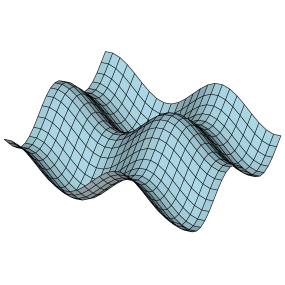
\includegraphics[height=7.5cm]{surf1.png}%
\else% TeXgraph version 1.989
\bgroup%
%\shorthandoff{;:!?}% uncomment if problem with babel
\pgfdeclarehorizontalshading[colorA,colorB]{myshading}{100bp}{color(0bp)=(colorA);color(75bp)=(colorB)}%
\pgfdeclareradialshading[colorA,colorB]{mysphereshading}{\pgfpoint{\GradCenterX bp}{\GradCenterY bp}}{color(0bp)=(colorA); color(35bp)=(colorB)}%
%\shorthandon{;:!?}% uncomment if problem with babel
\begin{tikzpicture}%
\pgfsetxvec{\pgfxy(0.5357,0)}%
\pgfsetyvec{\pgfxy(0,0.5357)}%
\useasboundingbox (-7,-7)--(7,7);
%image  (User)
\pgfsetstrokecolor{rgb,1:red,0;green,0;blue,0}%
\pgfsetlinewidth{0.4pt}%
\pgfsetroundjoin%
\pgfpathmoveto{\pgfxy(-1.8301,4.4912)}%
\pgfpathlineto{\pgfxy(-2.0385,3.9536)}\pgfpathlineto{\pgfxy(-1.6776,3.8778)}\pgfpathlineto{\pgfxy(-1.4693,4.4154)}\pgfclosepath%
\pgfsetfillcolor{rgb,1:red,0.6392;green,0.7961;blue,0.8471}%
\pgffillstroke%
\pgfpathmoveto{\pgfxy(-2.0385,3.9536)}%
\pgfpathlineto{\pgfxy(-2.2468,3.4352)}\pgfpathlineto{\pgfxy(-1.8859,3.3594)}\pgfpathlineto{\pgfxy(-1.6776,3.8778)}\pgfclosepath%
\pgfsetfillcolor{rgb,1:red,0.6353;green,0.7961;blue,0.8471}%
\pgffillstroke%
\pgfpathmoveto{\pgfxy(-1.4693,4.4154)}%
\pgfpathlineto{\pgfxy(-1.6776,3.8778)}\pgfpathlineto{\pgfxy(-1.3168,3.6551)}\pgfpathlineto{\pgfxy(-1.1084,4.1926)}\pgfclosepath%
\pgfsetfillcolor{rgb,1:red,0.6667;green,0.8314;blue,0.8863}%
\pgffillstroke%
\pgfpathmoveto{\pgfxy(-0.0259,2.9467)}%
\pgfpathlineto{\pgfxy(-0.2342,2.4092)}\pgfpathlineto{\pgfxy(0.1266,1.9799)}\pgfpathlineto{\pgfxy(0.3349,2.5174)}\pgfclosepath%
\pgfsetfillcolor{rgb,1:red,0.6706;green,0.8392;blue,0.8941}%
\pgffillstroke%
\pgfpathmoveto{\pgfxy(-0.3868,3.4091)}%
\pgfpathlineto{\pgfxy(-0.5951,2.8716)}\pgfpathlineto{\pgfxy(-0.2342,2.4092)}\pgfpathlineto{\pgfxy(-0.0259,2.9467)}\pgfclosepath%
\pgfsetfillcolor{rgb,1:red,0.6706;green,0.8353;blue,0.8902}%
\pgffillstroke%
\pgfpathmoveto{\pgfxy(0.3349,2.5174)}%
\pgfpathlineto{\pgfxy(0.1266,1.9799)}\pgfpathlineto{\pgfxy(0.4874,1.6393)}\pgfpathlineto{\pgfxy(0.6958,2.1768)}\pgfclosepath%
\pgfsetfillcolor{rgb,1:red,0.6745;green,0.8431;blue,0.8941}%
\pgffillstroke%
\pgfpathmoveto{\pgfxy(-1.1084,4.1926)}%
\pgfpathlineto{\pgfxy(-1.3168,3.6551)}\pgfpathlineto{\pgfxy(-0.9559,3.3057)}\pgfpathlineto{\pgfxy(-0.7476,3.8432)}\pgfclosepath%
\pgfsetfillcolor{rgb,1:red,0.6745;green,0.8431;blue,0.8941}%
\pgffillstroke%
\pgfpathmoveto{\pgfxy(-0.7476,3.8432)}%
\pgfpathlineto{\pgfxy(-0.9559,3.3057)}\pgfpathlineto{\pgfxy(-0.5951,2.8716)}\pgfpathlineto{\pgfxy(-0.3868,3.4091)}\pgfclosepath%
\pgfsetfillcolor{rgb,1:red,0.6706;green,0.8392;blue,0.8941}%
\pgffillstroke%
\pgfpathmoveto{\pgfxy(-2.2468,3.4352)}%
\pgfpathlineto{\pgfxy(-2.4551,2.9936)}\pgfpathlineto{\pgfxy(-2.0943,2.9178)}\pgfpathlineto{\pgfxy(-1.8859,3.3594)}\pgfclosepath%
\pgfsetfillcolor{rgb,1:red,0.6235;green,0.7804;blue,0.8314}%
\pgffillstroke%
\pgfpathmoveto{\pgfxy(-1.6776,3.8778)}%
\pgfpathlineto{\pgfxy(-1.8859,3.3594)}\pgfpathlineto{\pgfxy(-1.5251,3.1366)}\pgfpathlineto{\pgfxy(-1.3168,3.6551)}\pgfclosepath%
\pgfsetfillcolor{rgb,1:red,0.6667;green,0.8314;blue,0.8863}%
\pgffillstroke%
\pgfpathmoveto{\pgfxy(0.6958,2.1768)}%
\pgfpathlineto{\pgfxy(0.4874,1.6393)}\pgfpathlineto{\pgfxy(0.8483,1.4278)}\pgfpathlineto{\pgfxy(1.0566,1.9653)}\pgfclosepath%
\pgfsetfillcolor{rgb,1:red,0.6667;green,0.8314;blue,0.8863}%
\pgffillstroke%
\pgfpathmoveto{\pgfxy(-0.2342,2.4092)}%
\pgfpathlineto{\pgfxy(-0.4426,1.8907)}\pgfpathlineto{\pgfxy(-0.0817,1.4614)}\pgfpathlineto{\pgfxy(0.1266,1.9799)}\pgfclosepath%
\pgfsetfillcolor{rgb,1:red,0.6706;green,0.8353;blue,0.8902}%
\pgffillstroke%
\pgfpathmoveto{\pgfxy(-0.5951,2.8716)}%
\pgfpathlineto{\pgfxy(-0.8034,2.3531)}\pgfpathlineto{\pgfxy(-0.4426,1.8907)}\pgfpathlineto{\pgfxy(-0.2342,2.4092)}\pgfclosepath%
\pgfsetfillcolor{rgb,1:red,0.6706;green,0.8353;blue,0.8902}%
\pgffillstroke%
\pgfpathmoveto{\pgfxy(0.1266,1.9799)}%
\pgfpathlineto{\pgfxy(-0.0817,1.4614)}\pgfpathlineto{\pgfxy(0.2791,1.1208)}\pgfpathlineto{\pgfxy(0.4874,1.6393)}\pgfclosepath%
\pgfsetfillcolor{rgb,1:red,0.6745;green,0.8392;blue,0.8941}%
\pgffillstroke%
\pgfpathmoveto{\pgfxy(-1.3168,3.6551)}%
\pgfpathlineto{\pgfxy(-1.5251,3.1366)}\pgfpathlineto{\pgfxy(-1.1643,2.7872)}\pgfpathlineto{\pgfxy(-0.9559,3.3057)}\pgfclosepath%
\pgfsetfillcolor{rgb,1:red,0.6745;green,0.8392;blue,0.8941}%
\pgffillstroke%
\pgfpathmoveto{\pgfxy(-0.9559,3.3057)}%
\pgfpathlineto{\pgfxy(-1.1643,2.7872)}\pgfpathlineto{\pgfxy(-0.8034,2.3531)}\pgfpathlineto{\pgfxy(-0.5951,2.8716)}\pgfclosepath%
\pgfsetfillcolor{rgb,1:red,0.6706;green,0.8353;blue,0.8902}%
\pgffillstroke%
\pgfpathmoveto{\pgfxy(-1.8859,3.3594)}%
\pgfpathlineto{\pgfxy(-2.0943,2.9178)}\pgfpathlineto{\pgfxy(-1.7334,2.6951)}\pgfpathlineto{\pgfxy(-1.5251,3.1366)}\pgfclosepath%
\pgfsetfillcolor{rgb,1:red,0.6588;green,0.8235;blue,0.8745}%
\pgffillstroke%
\pgfpathmoveto{\pgfxy(0.4874,1.6393)}%
\pgfpathlineto{\pgfxy(0.2791,1.1208)}\pgfpathlineto{\pgfxy(0.64,0.9093)}\pgfpathlineto{\pgfxy(0.8483,1.4278)}\pgfclosepath%
\pgfsetfillcolor{rgb,1:red,0.6627;green,0.8314;blue,0.8824}%
\pgffillstroke%
\pgfpathmoveto{\pgfxy(-2.4551,2.9936)}%
\pgfpathlineto{\pgfxy(-2.6635,2.6737)}\pgfpathlineto{\pgfxy(-2.3026,2.5979)}\pgfpathlineto{\pgfxy(-2.0943,2.9178)}\pgfclosepath%
\pgfsetfillcolor{rgb,1:red,0.5882;green,0.7373;blue,0.7843}%
\pgffillstroke%
\pgfpathmoveto{\pgfxy(-0.4426,1.8907)}%
\pgfpathlineto{\pgfxy(-0.6509,1.4492)}\pgfpathlineto{\pgfxy(-0.2901,1.0199)}\pgfpathlineto{\pgfxy(-0.0817,1.4614)}\pgfclosepath%
\pgfsetfillcolor{rgb,1:red,0.6627;green,0.8275;blue,0.8784}%
\pgffillstroke%
\pgfpathmoveto{\pgfxy(1.0566,1.9653)}%
\pgfpathlineto{\pgfxy(0.8483,1.4278)}\pgfpathlineto{\pgfxy(1.2091,1.3638)}\pgfpathlineto{\pgfxy(1.4175,1.9014)}\pgfclosepath%
\pgfsetfillcolor{rgb,1:red,0.6353;green,0.7922;blue,0.8431}%
\pgffillstroke%
\pgfpathmoveto{\pgfxy(-0.8034,2.3531)}%
\pgfpathlineto{\pgfxy(-1.0118,1.9115)}\pgfpathlineto{\pgfxy(-0.6509,1.4492)}\pgfpathlineto{\pgfxy(-0.4426,1.8907)}\pgfclosepath%
\pgfsetfillcolor{rgb,1:red,0.6588;green,0.8235;blue,0.8745}%
\pgffillstroke%
\pgfpathmoveto{\pgfxy(-0.0817,1.4614)}%
\pgfpathlineto{\pgfxy(-0.2901,1.0199)}\pgfpathlineto{\pgfxy(0.0708,0.6793)}\pgfpathlineto{\pgfxy(0.2791,1.1208)}\pgfclosepath%
\pgfsetfillcolor{rgb,1:red,0.6627;green,0.8314;blue,0.8824}%
\pgffillstroke%
\pgfpathmoveto{\pgfxy(-1.5251,3.1366)}%
\pgfpathlineto{\pgfxy(-1.7334,2.6951)}\pgfpathlineto{\pgfxy(-1.3726,2.3457)}\pgfpathlineto{\pgfxy(-1.1643,2.7872)}\pgfclosepath%
\pgfsetfillcolor{rgb,1:red,0.6627;green,0.8314;blue,0.8824}%
\pgffillstroke%
\pgfpathmoveto{\pgfxy(-1.1643,2.7872)}%
\pgfpathlineto{\pgfxy(-1.3726,2.3457)}\pgfpathlineto{\pgfxy(-1.0118,1.9115)}\pgfpathlineto{\pgfxy(-0.8034,2.3531)}\pgfclosepath%
\pgfsetfillcolor{rgb,1:red,0.6627;green,0.8235;blue,0.8784}%
\pgffillstroke%
\pgfpathmoveto{\pgfxy(0.2791,1.1208)}%
\pgfpathlineto{\pgfxy(0.0708,0.6793)}\pgfpathlineto{\pgfxy(0.4316,0.4678)}\pgfpathlineto{\pgfxy(0.64,0.9093)}\pgfclosepath%
\pgfsetfillcolor{rgb,1:red,0.6588;green,0.8196;blue,0.8745}%
\pgffillstroke%
\pgfpathmoveto{\pgfxy(0.8483,1.4278)}%
\pgfpathlineto{\pgfxy(0.64,0.9093)}\pgfpathlineto{\pgfxy(1.0008,0.8454)}\pgfpathlineto{\pgfxy(1.2091,1.3638)}\pgfclosepath%
\pgfsetfillcolor{rgb,1:red,0.6314;green,0.7882;blue,0.8392}%
\pgffillstroke%
\pgfpathmoveto{\pgfxy(-2.0943,2.9178)}%
\pgfpathlineto{\pgfxy(-2.3026,2.5979)}\pgfpathlineto{\pgfxy(-1.9418,2.3751)}\pgfpathlineto{\pgfxy(-1.7334,2.6951)}\pgfclosepath%
\pgfsetfillcolor{rgb,1:red,0.6314;green,0.7882;blue,0.8392}%
\pgffillstroke%
\pgfpathmoveto{\pgfxy(-0.6509,1.4492)}%
\pgfpathlineto{\pgfxy(-0.8592,1.1292)}\pgfpathlineto{\pgfxy(-0.4984,0.6999)}\pgfpathlineto{\pgfxy(-0.2901,1.0199)}\pgfclosepath%
\pgfsetfillcolor{rgb,1:red,0.6353;green,0.7922;blue,0.8431}%
\pgffillstroke%
\pgfpathmoveto{\pgfxy(-1.0118,1.9115)}%
\pgfpathlineto{\pgfxy(-1.2201,1.5916)}\pgfpathlineto{\pgfxy(-0.8592,1.1292)}\pgfpathlineto{\pgfxy(-0.6509,1.4492)}\pgfclosepath%
\pgfsetfillcolor{rgb,1:red,0.6314;green,0.7882;blue,0.8392}%
\pgffillstroke%
\pgfpathmoveto{\pgfxy(-0.2901,1.0199)}%
\pgfpathlineto{\pgfxy(-0.4984,0.6999)}\pgfpathlineto{\pgfxy(-0.1376,0.3593)}\pgfpathlineto{\pgfxy(0.0708,0.6793)}\pgfclosepath%
\pgfsetfillcolor{rgb,1:red,0.6353;green,0.7961;blue,0.8471}%
\pgffillstroke%
\pgfpathmoveto{\pgfxy(-1.7334,2.6951)}%
\pgfpathlineto{\pgfxy(-1.9418,2.3751)}\pgfpathlineto{\pgfxy(-1.5809,2.0257)}\pgfpathlineto{\pgfxy(-1.3726,2.3457)}\pgfclosepath%
\pgfsetfillcolor{rgb,1:red,0.6353;green,0.7961;blue,0.8471}%
\pgffillstroke%
\pgfpathmoveto{\pgfxy(-1.3726,2.3457)}%
\pgfpathlineto{\pgfxy(-1.5809,2.0257)}\pgfpathlineto{\pgfxy(-1.2201,1.5916)}\pgfpathlineto{\pgfxy(-1.0118,1.9115)}\pgfclosepath%
\pgfsetfillcolor{rgb,1:red,0.6314;green,0.7922;blue,0.8431}%
\pgffillstroke%
\pgfpathmoveto{\pgfxy(1.4175,1.9014)}%
\pgfpathlineto{\pgfxy(1.2091,1.3638)}\pgfpathlineto{\pgfxy(1.57,1.4405)}\pgfpathlineto{\pgfxy(1.7783,1.978)}\pgfclosepath%
\pgfsetfillcolor{rgb,1:red,0.5843;green,0.7294;blue,0.7765}%
\pgffillstroke%
\pgfpathmoveto{\pgfxy(0.64,0.9093)}%
\pgfpathlineto{\pgfxy(0.4316,0.4678)}\pgfpathlineto{\pgfxy(0.7925,0.4038)}\pgfpathlineto{\pgfxy(1.0008,0.8454)}\pgfclosepath%
\pgfsetfillcolor{rgb,1:red,0.6196;green,0.7765;blue,0.8275}%
\pgffillstroke%
\pgfpathmoveto{\pgfxy(-2.6635,2.6737)}%
\pgfpathlineto{\pgfxy(-2.8718,2.4992)}\pgfpathlineto{\pgfxy(-2.5109,2.4234)}\pgfpathlineto{\pgfxy(-2.3026,2.5979)}\pgfclosepath%
\pgfsetfillcolor{rgb,1:red,0.4941;green,0.6157;blue,0.6549}%
\pgffillstroke%
\pgfpathmoveto{\pgfxy(0.0708,0.6793)}%
\pgfpathlineto{\pgfxy(-0.1376,0.3593)}\pgfpathlineto{\pgfxy(0.2233,0.1478)}\pgfpathlineto{\pgfxy(0.4316,0.4678)}\pgfclosepath%
\pgfsetfillcolor{rgb,1:red,0.6275;green,0.7843;blue,0.8353}%
\pgffillstroke%
\pgfpathmoveto{\pgfxy(1.2091,1.3638)}%
\pgfpathlineto{\pgfxy(1.0008,0.8454)}\pgfpathlineto{\pgfxy(1.3616,0.922)}\pgfpathlineto{\pgfxy(1.57,1.4405)}\pgfclosepath%
\pgfsetfillcolor{rgb,1:red,0.5804;green,0.7255;blue,0.7725}%
\pgffillstroke%
\pgfpathmoveto{\pgfxy(-2.3026,2.5979)}%
\pgfpathlineto{\pgfxy(-2.5109,2.4234)}\pgfpathlineto{\pgfxy(-2.1501,2.2006)}\pgfpathlineto{\pgfxy(-1.9418,2.3751)}\pgfclosepath%
\pgfsetfillcolor{rgb,1:red,0.5529;green,0.6902;blue,0.7333}%
\pgffillstroke%
\pgfpathmoveto{\pgfxy(0.4316,0.4678)}%
\pgfpathlineto{\pgfxy(0.2233,0.1478)}\pgfpathlineto{\pgfxy(0.5841,0.0839)}\pgfpathlineto{\pgfxy(0.7925,0.4038)}\pgfclosepath%
\pgfsetfillcolor{rgb,1:red,0.5843;green,0.7294;blue,0.7765}%
\pgffillstroke%
\pgfpathmoveto{\pgfxy(-0.8592,1.1292)}%
\pgfpathlineto{\pgfxy(-1.0676,0.9548)}\pgfpathlineto{\pgfxy(-0.7067,0.5255)}\pgfpathlineto{\pgfxy(-0.4984,0.6999)}\pgfclosepath%
\pgfsetfillcolor{rgb,1:red,0.5725;green,0.7137;blue,0.7608}%
\pgffillstroke%
\pgfpathmoveto{\pgfxy(-1.2201,1.5916)}%
\pgfpathlineto{\pgfxy(-1.4284,1.4171)}\pgfpathlineto{\pgfxy(-1.0676,0.9548)}\pgfpathlineto{\pgfxy(-0.8592,1.1292)}\pgfclosepath%
\pgfsetfillcolor{rgb,1:red,0.5725;green,0.7137;blue,0.7608}%
\pgffillstroke%
\pgfpathmoveto{\pgfxy(-0.4984,0.6999)}%
\pgfpathlineto{\pgfxy(-0.7067,0.5255)}\pgfpathlineto{\pgfxy(-0.3459,0.1848)}\pgfpathlineto{\pgfxy(-0.1376,0.3593)}\pgfclosepath%
\pgfsetfillcolor{rgb,1:red,0.5686;green,0.7098;blue,0.7569}%
\pgffillstroke%
\pgfpathmoveto{\pgfxy(-1.9418,2.3751)}%
\pgfpathlineto{\pgfxy(-2.1501,2.2006)}\pgfpathlineto{\pgfxy(-1.7893,1.8512)}\pgfpathlineto{\pgfxy(-1.5809,2.0257)}\pgfclosepath%
\pgfsetfillcolor{rgb,1:red,0.5686;green,0.7098;blue,0.7569}%
\pgffillstroke%
\pgfpathmoveto{\pgfxy(1.0008,0.8454)}%
\pgfpathlineto{\pgfxy(0.7925,0.4038)}\pgfpathlineto{\pgfxy(1.1533,0.4805)}\pgfpathlineto{\pgfxy(1.3616,0.922)}\pgfclosepath%
\pgfsetfillcolor{rgb,1:red,0.5608;green,0.698;blue,0.7451}%
\pgffillstroke%
\pgfpathmoveto{\pgfxy(-1.5809,2.0257)}%
\pgfpathlineto{\pgfxy(-1.7893,1.8512)}\pgfpathlineto{\pgfxy(-1.4284,1.4171)}\pgfpathlineto{\pgfxy(-1.2201,1.5916)}\pgfclosepath%
\pgfsetfillcolor{rgb,1:red,0.5725;green,0.7137;blue,0.7608}%
\pgffillstroke%
\pgfpathmoveto{\pgfxy(1.7783,1.978)}%
\pgfpathlineto{\pgfxy(1.57,1.4405)}\pgfpathlineto{\pgfxy(1.9308,1.6269)}\pgfpathlineto{\pgfxy(2.1392,2.1644)}\pgfclosepath%
\pgfsetfillcolor{rgb,1:red,0.5333;green,0.6667;blue,0.7098}%
\pgffillstroke%
\pgfpathmoveto{\pgfxy(-0.1376,0.3593)}%
\pgfpathlineto{\pgfxy(-0.3459,0.1848)}\pgfpathlineto{\pgfxy(0.015,-0.0266)}\pgfpathlineto{\pgfxy(0.2233,0.1478)}\pgfclosepath%
\pgfsetfillcolor{rgb,1:red,0.549;green,0.6863;blue,0.7294}%
\pgffillstroke%
\pgfpathmoveto{\pgfxy(-2.8718,2.4992)}%
\pgfpathlineto{\pgfxy(-3.0801,2.4692)}\pgfpathlineto{\pgfxy(-2.7193,2.3934)}\pgfpathlineto{\pgfxy(-2.5109,2.4234)}\pgfclosepath%
\pgfsetfillcolor{rgb,1:red,0.3098;green,0.3882;blue,0.4118}%
\pgffillstroke%
\pgfpathmoveto{\pgfxy(1.57,1.4405)}%
\pgfpathlineto{\pgfxy(1.3616,0.922)}\pgfpathlineto{\pgfxy(1.7225,1.1084)}\pgfpathlineto{\pgfxy(1.9308,1.6269)}\pgfclosepath%
\pgfsetfillcolor{rgb,1:red,0.5294;green,0.6588;blue,0.702}%
\pgffillstroke%
\pgfpathmoveto{\pgfxy(0.7925,0.4038)}%
\pgfpathlineto{\pgfxy(0.5841,0.0839)}\pgfpathlineto{\pgfxy(0.945,0.1605)}\pgfpathlineto{\pgfxy(1.1533,0.4805)}\pgfclosepath%
\pgfsetfillcolor{rgb,1:red,0.5059;green,0.6353;blue,0.6745}%
\pgffillstroke%
\pgfpathmoveto{\pgfxy(0.2233,0.1478)}%
\pgfpathlineto{\pgfxy(0.015,-0.0266)}\pgfpathlineto{\pgfxy(0.3758,-0.0906)}\pgfpathlineto{\pgfxy(0.5841,0.0839)}\pgfclosepath%
\pgfsetfillcolor{rgb,1:red,0.4863;green,0.6078;blue,0.6471}%
\pgffillstroke%
\pgfpathmoveto{\pgfxy(-2.5109,2.4234)}%
\pgfpathlineto{\pgfxy(-2.7193,2.3934)}\pgfpathlineto{\pgfxy(-2.3584,2.1706)}\pgfpathlineto{\pgfxy(-2.1501,2.2006)}\pgfclosepath%
\pgfsetfillcolor{rgb,1:red,0.4157;green,0.5176;blue,0.549}%
\pgffillstroke%
\pgfpathmoveto{\pgfxy(1.3616,0.922)}%
\pgfpathlineto{\pgfxy(1.1533,0.4805)}\pgfpathlineto{\pgfxy(1.5142,0.6668)}\pgfpathlineto{\pgfxy(1.7225,1.1084)}\pgfclosepath%
\pgfsetfillcolor{rgb,1:red,0.502;green,0.6275;blue,0.6667}%
\pgffillstroke%
\pgfpathmoveto{\pgfxy(-1.0676,0.9548)}%
\pgfpathlineto{\pgfxy(-1.2759,0.9247)}\pgfpathlineto{\pgfxy(-0.9151,0.4954)}\pgfpathlineto{\pgfxy(-0.7067,0.5255)}\pgfclosepath%
\pgfsetfillcolor{rgb,1:red,0.4745;green,0.5922;blue,0.6314}%
\pgffillstroke%
\pgfpathmoveto{\pgfxy(-1.4284,1.4171)}%
\pgfpathlineto{\pgfxy(-1.6368,1.3871)}\pgfpathlineto{\pgfxy(-1.2759,0.9247)}\pgfpathlineto{\pgfxy(-1.0676,0.9548)}\pgfclosepath%
\pgfsetfillcolor{rgb,1:red,0.4784;green,0.6;blue,0.6392}%
\pgffillstroke%
\pgfpathmoveto{\pgfxy(-0.7067,0.5255)}%
\pgfpathlineto{\pgfxy(-0.9151,0.4954)}\pgfpathlineto{\pgfxy(-0.5542,0.1548)}\pgfpathlineto{\pgfxy(-0.3459,0.1848)}\pgfclosepath%
\pgfsetfillcolor{rgb,1:red,0.4549;green,0.5686;blue,0.6078}%
\pgffillstroke%
\pgfpathmoveto{\pgfxy(-2.1501,2.2006)}%
\pgfpathlineto{\pgfxy(-2.3584,2.1706)}\pgfpathlineto{\pgfxy(-1.9976,1.8212)}\pgfpathlineto{\pgfxy(-1.7893,1.8512)}\pgfclosepath%
\pgfsetfillcolor{rgb,1:red,0.4588;green,0.5725;blue,0.6118}%
\pgffillstroke%
\pgfpathmoveto{\pgfxy(-1.7893,1.8512)}%
\pgfpathlineto{\pgfxy(-1.9976,1.8212)}\pgfpathlineto{\pgfxy(-1.6368,1.3871)}\pgfpathlineto{\pgfxy(-1.4284,1.4171)}\pgfclosepath%
\pgfsetfillcolor{rgb,1:red,0.4745;green,0.5922;blue,0.6314}%
\pgffillstroke%
\pgfpathmoveto{\pgfxy(-0.3459,0.1848)}%
\pgfpathlineto{\pgfxy(-0.5542,0.1548)}\pgfpathlineto{\pgfxy(-0.1934,-0.0567)}\pgfpathlineto{\pgfxy(0.015,-0.0266)}\pgfclosepath%
\pgfsetfillcolor{rgb,1:red,0.4078;green,0.5098;blue,0.5451}%
\pgffillstroke%
\pgfpathmoveto{\pgfxy(2.1392,2.1644)}%
\pgfpathlineto{\pgfxy(1.9308,1.6269)}\pgfpathlineto{\pgfxy(2.2917,1.8732)}\pgfpathlineto{\pgfxy(2.5,2.4107)}\pgfclosepath%
\pgfsetfillcolor{rgb,1:red,0.5059;green,0.6314;blue,0.6745}%
\pgffillstroke%
\pgfpathmoveto{\pgfxy(0.5841,0.0839)}%
\pgfpathlineto{\pgfxy(0.3758,-0.0906)}\pgfpathlineto{\pgfxy(0.7366,-0.0139)}\pgfpathlineto{\pgfxy(0.945,0.1605)}\pgfclosepath%
\pgfsetfillcolor{rgb,1:red,0.3843;green,0.4784;blue,0.5098}%
\pgffillstroke%
\pgfpathmoveto{\pgfxy(1.1533,0.4805)}%
\pgfpathlineto{\pgfxy(0.945,0.1605)}\pgfpathlineto{\pgfxy(1.3058,0.3469)}\pgfpathlineto{\pgfxy(1.5142,0.6668)}\pgfclosepath%
\pgfsetfillcolor{rgb,1:red,0.4353;green,0.5412;blue,0.5765}%
\pgffillstroke%
\pgfpathmoveto{\pgfxy(1.9308,1.6269)}%
\pgfpathlineto{\pgfxy(1.7225,1.1084)}\pgfpathlineto{\pgfxy(2.0833,1.3547)}\pgfpathlineto{\pgfxy(2.2917,1.8732)}\pgfclosepath%
\pgfsetfillcolor{rgb,1:red,0.498;green,0.6235;blue,0.6627}%
\pgffillstroke%
\pgfpathmoveto{\pgfxy(-3.0801,2.4692)}%
\pgfpathlineto{\pgfxy(-3.2885,2.5579)}\pgfpathlineto{\pgfxy(-2.9276,2.4821)}\pgfpathlineto{\pgfxy(-2.7193,2.3934)}\pgfclosepath%
\pgfsetfillcolor{rgb,1:red,0.2941;green,0.3255;blue,0.3373}%
\pgffillstroke%
\pgfpathmoveto{\pgfxy(0.015,-0.0266)}%
\pgfpathlineto{\pgfxy(-0.1934,-0.0567)}\pgfpathlineto{\pgfxy(0.1675,-0.1206)}\pgfpathlineto{\pgfxy(0.3758,-0.0906)}\pgfclosepath%
\pgfsetfillcolor{rgb,1:red,0.298;green,0.3725;blue,0.3961}%
\pgffillstroke%
\pgfpathmoveto{\pgfxy(1.7225,1.1084)}%
\pgfpathlineto{\pgfxy(1.5142,0.6668)}\pgfpathlineto{\pgfxy(1.875,0.9132)}\pgfpathlineto{\pgfxy(2.0833,1.3547)}\pgfclosepath%
\pgfsetfillcolor{rgb,1:red,0.4667;green,0.5843;blue,0.6235}%
\pgffillstroke%
\pgfpathmoveto{\pgfxy(-2.7193,2.3934)}%
\pgfpathlineto{\pgfxy(-2.9276,2.4821)}\pgfpathlineto{\pgfxy(-2.5668,2.2593)}\pgfpathlineto{\pgfxy(-2.3584,2.1706)}\pgfclosepath%
\pgfsetfillcolor{rgb,1:red,0.2275;green,0.2824;blue,0.302}%
\pgffillstroke%
\pgfpathmoveto{\pgfxy(-1.2759,0.9247)}%
\pgfpathlineto{\pgfxy(-1.4842,1.0134)}\pgfpathlineto{\pgfxy(-1.1234,0.5841)}\pgfpathlineto{\pgfxy(-0.9151,0.4954)}\pgfclosepath%
\pgfsetfillcolor{rgb,1:red,0.3686;green,0.4588;blue,0.4863}%
\pgffillstroke%
\pgfpathmoveto{\pgfxy(-1.6368,1.3871)}%
\pgfpathlineto{\pgfxy(-1.8451,1.4758)}\pgfpathlineto{\pgfxy(-1.4842,1.0134)}\pgfpathlineto{\pgfxy(-1.2759,0.9247)}\pgfclosepath%
\pgfsetfillcolor{rgb,1:red,0.3765;green,0.4706;blue,0.502}%
\pgffillstroke%
\pgfpathmoveto{\pgfxy(-0.9151,0.4954)}%
\pgfpathlineto{\pgfxy(-1.1234,0.5841)}\pgfpathlineto{\pgfxy(-0.7626,0.2435)}\pgfpathlineto{\pgfxy(-0.5542,0.1548)}\pgfclosepath%
\pgfsetfillcolor{rgb,1:red,0.3255;green,0.4078;blue,0.4314}%
\pgffillstroke%
\pgfpathmoveto{\pgfxy(-2.3584,2.1706)}%
\pgfpathlineto{\pgfxy(-2.5668,2.2593)}\pgfpathlineto{\pgfxy(-2.2059,1.9099)}\pgfpathlineto{\pgfxy(-1.9976,1.8212)}\pgfclosepath%
\pgfsetfillcolor{rgb,1:red,0.3294;green,0.4118;blue,0.4392}%
\pgffillstroke%
\pgfpathmoveto{\pgfxy(0.945,0.1605)}%
\pgfpathlineto{\pgfxy(0.7366,-0.0139)}\pgfpathlineto{\pgfxy(1.0975,0.1724)}\pgfpathlineto{\pgfxy(1.3058,0.3469)}\pgfclosepath%
\pgfsetfillcolor{rgb,1:red,0.2784;green,0.349;blue,0.3725}%
\pgffillstroke%
\pgfpathmoveto{\pgfxy(-1.9976,1.8212)}%
\pgfpathlineto{\pgfxy(-2.2059,1.9099)}\pgfpathlineto{\pgfxy(-1.8451,1.4758)}\pgfpathlineto{\pgfxy(-1.6368,1.3871)}\pgfclosepath%
\pgfsetfillcolor{rgb,1:red,0.3686;green,0.4588;blue,0.4902}%
\pgffillstroke%
\pgfpathmoveto{\pgfxy(2.5,2.4107)}%
\pgfpathlineto{\pgfxy(2.2917,1.8732)}\pgfpathlineto{\pgfxy(2.6525,2.1195)}\pgfpathlineto{\pgfxy(2.8608,2.657)}\pgfclosepath%
\pgfsetfillcolor{rgb,1:red,0.5059;green,0.6314;blue,0.6745}%
\pgffillstroke%
\pgfpathmoveto{\pgfxy(0.3758,-0.0906)}%
\pgfpathlineto{\pgfxy(0.1675,-0.1206)}\pgfpathlineto{\pgfxy(0.5283,-0.044)}\pgfpathlineto{\pgfxy(0.7366,-0.0139)}\pgfclosepath%
\pgfsetfillcolor{rgb,1:red,0.1922;green,0.2118;blue,0.2157}%
\pgffillstroke%
\pgfpathmoveto{\pgfxy(-0.5542,0.1548)}%
\pgfpathlineto{\pgfxy(-0.7626,0.2435)}\pgfpathlineto{\pgfxy(-0.4017,0.032)}\pgfpathlineto{\pgfxy(-0.1934,-0.0567)}\pgfclosepath%
\pgfsetfillcolor{rgb,1:red,0.2118;green,0.2627;blue,0.2824}%
\pgffillstroke%
\pgfpathmoveto{\pgfxy(1.5142,0.6668)}%
\pgfpathlineto{\pgfxy(1.3058,0.3469)}\pgfpathlineto{\pgfxy(1.6667,0.5932)}\pgfpathlineto{\pgfxy(1.875,0.9132)}\pgfclosepath%
\pgfsetfillcolor{rgb,1:red,0.3922;green,0.4902;blue,0.5216}%
\pgffillstroke%
\pgfpathmoveto{\pgfxy(2.2917,1.8732)}%
\pgfpathlineto{\pgfxy(2.0833,1.3547)}\pgfpathlineto{\pgfxy(2.4442,1.601)}\pgfpathlineto{\pgfxy(2.6525,2.1195)}\pgfclosepath%
\pgfsetfillcolor{rgb,1:red,0.498;green,0.6235;blue,0.6627}%
\pgffillstroke%
\pgfpathmoveto{\pgfxy(-0.1934,-0.0567)}%
\pgfpathlineto{\pgfxy(-0.4017,0.032)}\pgfpathlineto{\pgfxy(-0.0409,-0.0319)}\pgfpathlineto{\pgfxy(0.1675,-0.1206)}\pgfclosepath%
\pgfsetfillcolor{rgb,1:red,0.3137;green,0.3451;blue,0.3569}%
\pgffillstroke%
\pgfpathmoveto{\pgfxy(-3.2885,2.5579)}%
\pgfpathlineto{\pgfxy(-3.4968,2.7192)}\pgfpathlineto{\pgfxy(-3.1359,2.6434)}\pgfpathlineto{\pgfxy(-2.9276,2.4821)}\pgfclosepath%
\pgfsetfillcolor{rgb,1:red,0.4196;green,0.4627;blue,0.4745}%
\pgffillstroke%
\pgfpathmoveto{\pgfxy(2.0833,1.3547)}%
\pgfpathlineto{\pgfxy(1.875,0.9132)}\pgfpathlineto{\pgfxy(2.2358,1.1595)}\pgfpathlineto{\pgfxy(2.4442,1.601)}\pgfclosepath%
\pgfsetfillcolor{rgb,1:red,0.4667;green,0.5843;blue,0.6235}%
\pgffillstroke%
\pgfpathmoveto{\pgfxy(0.7366,-0.0139)}%
\pgfpathlineto{\pgfxy(0.5283,-0.044)}\pgfpathlineto{\pgfxy(0.8892,0.1424)}\pgfpathlineto{\pgfxy(1.0975,0.1724)}\pgfclosepath%
\pgfsetfillcolor{rgb,1:red,0.3569;green,0.3922;blue,0.4039}%
\pgffillstroke%
\pgfpathmoveto{\pgfxy(1.3058,0.3469)}%
\pgfpathlineto{\pgfxy(1.0975,0.1724)}\pgfpathlineto{\pgfxy(1.4583,0.4187)}\pgfpathlineto{\pgfxy(1.6667,0.5932)}\pgfclosepath%
\pgfsetfillcolor{rgb,1:red,0.2;green,0.251;blue,0.2667}%
\pgffillstroke%
\pgfpathmoveto{\pgfxy(2.8608,2.657)}%
\pgfpathlineto{\pgfxy(2.6525,2.1195)}\pgfpathlineto{\pgfxy(3.0134,2.3059)}\pgfpathlineto{\pgfxy(3.2217,2.8434)}\pgfclosepath%
\pgfsetfillcolor{rgb,1:red,0.5333;green,0.6667;blue,0.7098}%
\pgffillstroke%
\pgfpathmoveto{\pgfxy(-2.9276,2.4821)}%
\pgfpathlineto{\pgfxy(-3.1359,2.6434)}\pgfpathlineto{\pgfxy(-2.7751,2.4207)}\pgfpathlineto{\pgfxy(-2.5668,2.2593)}\pgfclosepath%
\pgfsetfillcolor{rgb,1:red,0.2471;green,0.2745;blue,0.2824}%
\pgffillstroke%
\pgfpathmoveto{\pgfxy(-1.4842,1.0134)}%
\pgfpathlineto{\pgfxy(-1.6926,1.1748)}\pgfpathlineto{\pgfxy(-1.3317,0.7455)}\pgfpathlineto{\pgfxy(-1.1234,0.5841)}\pgfclosepath%
\pgfsetfillcolor{rgb,1:red,0.2784;green,0.349;blue,0.3725}%
\pgffillstroke%
\pgfpathmoveto{\pgfxy(1.875,0.9132)}%
\pgfpathlineto{\pgfxy(1.6667,0.5932)}\pgfpathlineto{\pgfxy(2.0275,0.8395)}\pgfpathlineto{\pgfxy(2.2358,1.1595)}\pgfclosepath%
\pgfsetfillcolor{rgb,1:red,0.3922;green,0.4902;blue,0.5216}%
\pgffillstroke%
\pgfpathmoveto{\pgfxy(0.1675,-0.1206)}%
\pgfpathlineto{\pgfxy(-0.0409,-0.0319)}\pgfpathlineto{\pgfxy(0.32,0.0447)}\pgfpathlineto{\pgfxy(0.5283,-0.044)}\pgfclosepath%
\pgfsetfillcolor{rgb,1:red,0.4431;green,0.4902;blue,0.5059}%
\pgffillstroke%
\pgfpathmoveto{\pgfxy(-1.8451,1.4758)}%
\pgfpathlineto{\pgfxy(-2.0534,1.6372)}\pgfpathlineto{\pgfxy(-1.6926,1.1748)}\pgfpathlineto{\pgfxy(-1.4842,1.0134)}\pgfclosepath%
\pgfsetfillcolor{rgb,1:red,0.298;green,0.3725;blue,0.3961}%
\pgffillstroke%
\pgfpathmoveto{\pgfxy(-1.1234,0.5841)}%
\pgfpathlineto{\pgfxy(-1.3317,0.7455)}\pgfpathlineto{\pgfxy(-0.9709,0.4049)}\pgfpathlineto{\pgfxy(-0.7626,0.2435)}\pgfclosepath%
\pgfsetfillcolor{rgb,1:red,0.2;green,0.251;blue,0.2667}%
\pgffillstroke%
\pgfpathmoveto{\pgfxy(-2.5668,2.2593)}%
\pgfpathlineto{\pgfxy(-2.7751,2.4207)}\pgfpathlineto{\pgfxy(-2.4143,2.0713)}\pgfpathlineto{\pgfxy(-2.2059,1.9099)}\pgfclosepath%
\pgfsetfillcolor{rgb,1:red,0.2118;green,0.2667;blue,0.2824}%
\pgffillstroke%
\pgfpathmoveto{\pgfxy(-2.2059,1.9099)}%
\pgfpathlineto{\pgfxy(-2.4143,2.0713)}\pgfpathlineto{\pgfxy(-2.0534,1.6372)}\pgfpathlineto{\pgfxy(-1.8451,1.4758)}\pgfclosepath%
\pgfsetfillcolor{rgb,1:red,0.2824;green,0.3529;blue,0.3765}%
\pgffillstroke%
\pgfpathmoveto{\pgfxy(2.6525,2.1195)}%
\pgfpathlineto{\pgfxy(2.4442,1.601)}\pgfpathlineto{\pgfxy(2.805,1.7874)}\pgfpathlineto{\pgfxy(3.0134,2.3059)}\pgfclosepath%
\pgfsetfillcolor{rgb,1:red,0.5294;green,0.6588;blue,0.702}%
\pgffillstroke%
\pgfpathmoveto{\pgfxy(-0.7626,0.2435)}%
\pgfpathlineto{\pgfxy(-0.9709,0.4049)}\pgfpathlineto{\pgfxy(-0.61,0.1934)}\pgfpathlineto{\pgfxy(-0.4017,0.032)}\pgfclosepath%
\pgfsetfillcolor{rgb,1:red,0.2667;green,0.2941;blue,0.302}%
\pgffillstroke%
\pgfpathmoveto{\pgfxy(2.4442,1.601)}%
\pgfpathlineto{\pgfxy(2.2358,1.1595)}\pgfpathlineto{\pgfxy(2.5967,1.3459)}\pgfpathlineto{\pgfxy(2.805,1.7874)}\pgfclosepath%
\pgfsetfillcolor{rgb,1:red,0.502;green,0.6275;blue,0.6667}%
\pgffillstroke%
\pgfpathmoveto{\pgfxy(3.2217,2.8434)}%
\pgfpathlineto{\pgfxy(3.0134,2.3059)}\pgfpathlineto{\pgfxy(3.3742,2.3825)}\pgfpathlineto{\pgfxy(3.5825,2.9201)}\pgfclosepath%
\pgfsetfillcolor{rgb,1:red,0.5843;green,0.7294;blue,0.7765}%
\pgffillstroke%
\pgfpathmoveto{\pgfxy(-0.4017,0.032)}%
\pgfpathlineto{\pgfxy(-0.61,0.1934)}\pgfpathlineto{\pgfxy(-0.2492,0.1294)}\pgfpathlineto{\pgfxy(-0.0409,-0.0319)}\pgfclosepath%
\pgfsetfillcolor{rgb,1:red,0.4275;green,0.4706;blue,0.4863}%
\pgffillstroke%
\pgfpathmoveto{\pgfxy(1.0975,0.1724)}%
\pgfpathlineto{\pgfxy(0.8892,0.1424)}\pgfpathlineto{\pgfxy(1.25,0.3887)}\pgfpathlineto{\pgfxy(1.4583,0.4187)}\pgfclosepath%
\pgfsetfillcolor{rgb,1:red,0.4;green,0.4431;blue,0.4549}%
\pgffillstroke%
\pgfpathmoveto{\pgfxy(1.6667,0.5932)}%
\pgfpathlineto{\pgfxy(1.4583,0.4187)}\pgfpathlineto{\pgfxy(1.8192,0.6651)}\pgfpathlineto{\pgfxy(2.0275,0.8395)}\pgfclosepath%
\pgfsetfillcolor{rgb,1:red,0.2;green,0.251;blue,0.2667}%
\pgffillstroke%
\pgfpathmoveto{\pgfxy(-3.4968,2.7192)}%
\pgfpathlineto{\pgfxy(-3.7051,2.8948)}\pgfpathlineto{\pgfxy(-3.3443,2.819)}\pgfpathlineto{\pgfxy(-3.1359,2.6434)}\pgfclosepath%
\pgfsetfillcolor{rgb,1:red,0.4353;green,0.4784;blue,0.4941}%
\pgffillstroke%
\pgfpathmoveto{\pgfxy(0.5283,-0.044)}%
\pgfpathlineto{\pgfxy(0.32,0.0447)}\pgfpathlineto{\pgfxy(0.6808,0.2311)}\pgfpathlineto{\pgfxy(0.8892,0.1424)}\pgfclosepath%
\pgfsetfillcolor{rgb,1:red,0.498;green,0.549;blue,0.5647}%
\pgffillstroke%
\pgfpathmoveto{\pgfxy(3.0134,2.3059)}%
\pgfpathlineto{\pgfxy(2.805,1.7874)}\pgfpathlineto{\pgfxy(3.1659,1.8641)}\pgfpathlineto{\pgfxy(3.3742,2.3825)}\pgfclosepath%
\pgfsetfillcolor{rgb,1:red,0.5804;green,0.7255;blue,0.7725}%
\pgffillstroke%
\pgfpathmoveto{\pgfxy(2.2358,1.1595)}%
\pgfpathlineto{\pgfxy(2.0275,0.8395)}\pgfpathlineto{\pgfxy(2.3884,1.0259)}\pgfpathlineto{\pgfxy(2.5967,1.3459)}\pgfclosepath%
\pgfsetfillcolor{rgb,1:red,0.4353;green,0.5412;blue,0.5765}%
\pgffillstroke%
\pgfpathmoveto{\pgfxy(-3.1359,2.6434)}%
\pgfpathlineto{\pgfxy(-3.3443,2.819)}\pgfpathlineto{\pgfxy(-2.9834,2.5962)}\pgfpathlineto{\pgfxy(-2.7751,2.4207)}\pgfclosepath%
\pgfsetfillcolor{rgb,1:red,0.2863;green,0.3137;blue,0.3216}%
\pgffillstroke%
\pgfpathmoveto{\pgfxy(3.5825,2.9201)}%
\pgfpathlineto{\pgfxy(3.3742,2.3825)}\pgfpathlineto{\pgfxy(3.735,2.3186)}\pgfpathlineto{\pgfxy(3.9434,2.8561)}\pgfclosepath%
\pgfsetfillcolor{rgb,1:red,0.6353;green,0.7922;blue,0.8431}%
\pgffillstroke%
\pgfpathmoveto{\pgfxy(2.805,1.7874)}%
\pgfpathlineto{\pgfxy(2.5967,1.3459)}\pgfpathlineto{\pgfxy(2.9575,1.4225)}\pgfpathlineto{\pgfxy(3.1659,1.8641)}\pgfclosepath%
\pgfsetfillcolor{rgb,1:red,0.5608;green,0.698;blue,0.7451}%
\pgffillstroke%
\pgfpathmoveto{\pgfxy(-0.0409,-0.0319)}%
\pgfpathlineto{\pgfxy(-0.2492,0.1294)}\pgfpathlineto{\pgfxy(0.1116,0.2061)}\pgfpathlineto{\pgfxy(0.32,0.0447)}\pgfclosepath%
\pgfsetfillcolor{rgb,1:red,0.5098;green,0.5647;blue,0.5804}%
\pgffillstroke%
\pgfpathmoveto{\pgfxy(-1.6926,1.1748)}%
\pgfpathlineto{\pgfxy(-1.9009,1.3504)}\pgfpathlineto{\pgfxy(-1.5401,0.9211)}\pgfpathlineto{\pgfxy(-1.3317,0.7455)}\pgfclosepath%
\pgfsetfillcolor{rgb,1:red,0.2588;green,0.3216;blue,0.3451}%
\pgffillstroke%
\pgfpathmoveto{\pgfxy(-2.0534,1.6372)}%
\pgfpathlineto{\pgfxy(-2.2618,1.8127)}\pgfpathlineto{\pgfxy(-1.9009,1.3504)}\pgfpathlineto{\pgfxy(-1.6926,1.1748)}\pgfclosepath%
\pgfsetfillcolor{rgb,1:red,0.2824;green,0.349;blue,0.3725}%
\pgffillstroke%
\pgfpathmoveto{\pgfxy(-1.3317,0.7455)}%
\pgfpathlineto{\pgfxy(-1.5401,0.9211)}\pgfpathlineto{\pgfxy(-1.1792,0.5804)}\pgfpathlineto{\pgfxy(-0.9709,0.4049)}\pgfclosepath%
\pgfsetfillcolor{rgb,1:red,0.1647;green,0.2039;blue,0.2157}%
\pgffillstroke%
\pgfpathmoveto{\pgfxy(-2.7751,2.4207)}%
\pgfpathlineto{\pgfxy(-2.9834,2.5962)}\pgfpathlineto{\pgfxy(-2.6226,2.2468)}\pgfpathlineto{\pgfxy(-2.4143,2.0713)}\pgfclosepath%
\pgfsetfillcolor{rgb,1:red,0.1765;green,0.2196;blue,0.2353}%
\pgffillstroke%
\pgfpathmoveto{\pgfxy(-2.4143,2.0713)}%
\pgfpathlineto{\pgfxy(-2.6226,2.2468)}\pgfpathlineto{\pgfxy(-2.2618,1.8127)}\pgfpathlineto{\pgfxy(-2.0534,1.6372)}\pgfclosepath%
\pgfsetfillcolor{rgb,1:red,0.2627;green,0.3294;blue,0.349}%
\pgffillstroke%
\pgfpathmoveto{\pgfxy(3.3742,2.3825)}%
\pgfpathlineto{\pgfxy(3.1659,1.8641)}\pgfpathlineto{\pgfxy(3.5267,1.8001)}\pgfpathlineto{\pgfxy(3.735,2.3186)}\pgfclosepath%
\pgfsetfillcolor{rgb,1:red,0.6314;green,0.7882;blue,0.8392}%
\pgffillstroke%
\pgfpathmoveto{\pgfxy(-0.9709,0.4049)}%
\pgfpathlineto{\pgfxy(-1.1792,0.5804)}\pgfpathlineto{\pgfxy(-0.8184,0.369)}\pgfpathlineto{\pgfxy(-0.61,0.1934)}\pgfclosepath%
\pgfsetfillcolor{rgb,1:red,0.302;green,0.3294;blue,0.3412}%
\pgffillstroke%
\pgfpathmoveto{\pgfxy(1.4583,0.4187)}%
\pgfpathlineto{\pgfxy(1.25,0.3887)}\pgfpathlineto{\pgfxy(1.6108,0.635)}\pgfpathlineto{\pgfxy(1.8192,0.6651)}\pgfclosepath%
\pgfsetfillcolor{rgb,1:red,0.4;green,0.4431;blue,0.4549}%
\pgffillstroke%
\pgfpathmoveto{\pgfxy(3.9434,2.8561)}%
\pgfpathlineto{\pgfxy(3.735,2.3186)}\pgfpathlineto{\pgfxy(4.0959,2.1071)}\pgfpathlineto{\pgfxy(4.3042,2.6446)}\pgfclosepath%
\pgfsetfillcolor{rgb,1:red,0.6667;green,0.8314;blue,0.8863}%
\pgffillstroke%
\pgfpathmoveto{\pgfxy(2.0275,0.8395)}%
\pgfpathlineto{\pgfxy(1.8192,0.6651)}\pgfpathlineto{\pgfxy(2.18,0.8514)}\pgfpathlineto{\pgfxy(2.3884,1.0259)}\pgfclosepath%
\pgfsetfillcolor{rgb,1:red,0.2784;green,0.349;blue,0.3725}%
\pgffillstroke%
\pgfpathmoveto{\pgfxy(2.5967,1.3459)}%
\pgfpathlineto{\pgfxy(2.3884,1.0259)}\pgfpathlineto{\pgfxy(2.7492,1.1026)}\pgfpathlineto{\pgfxy(2.9575,1.4225)}\pgfclosepath%
\pgfsetfillcolor{rgb,1:red,0.5059;green,0.6353;blue,0.6745}%
\pgffillstroke%
\pgfpathmoveto{\pgfxy(0.8892,0.1424)}%
\pgfpathlineto{\pgfxy(0.6808,0.2311)}\pgfpathlineto{\pgfxy(1.0417,0.4774)}\pgfpathlineto{\pgfxy(1.25,0.3887)}\pgfclosepath%
\pgfsetfillcolor{rgb,1:red,0.5176;green,0.5725;blue,0.5882}%
\pgffillstroke%
\pgfpathmoveto{\pgfxy(5.3868,1.4124)}%
\pgfpathlineto{\pgfxy(5.1784,0.8748)}\pgfpathlineto{\pgfxy(5.5393,0.4407)}\pgfpathlineto{\pgfxy(5.7476,0.9782)}\pgfclosepath%
\pgfsetfillcolor{rgb,1:red,0.6706;green,0.8392;blue,0.8941}%
\pgffillstroke%
\pgfpathmoveto{\pgfxy(5.7476,0.9782)}%
\pgfpathlineto{\pgfxy(5.5393,0.4407)}\pgfpathlineto{\pgfxy(5.9001,0.0913)}\pgfpathlineto{\pgfxy(6.1084,0.6288)}\pgfclosepath%
\pgfsetfillcolor{rgb,1:red,0.6745;green,0.8431;blue,0.8941}%
\pgffillstroke%
\pgfpathmoveto{\pgfxy(4.3042,2.6446)}%
\pgfpathlineto{\pgfxy(4.0959,2.1071)}\pgfpathlineto{\pgfxy(4.4567,1.7665)}\pgfpathlineto{\pgfxy(4.6651,2.304)}\pgfclosepath%
\pgfsetfillcolor{rgb,1:red,0.6745;green,0.8431;blue,0.8941}%
\pgffillstroke%
\pgfpathmoveto{\pgfxy(5.0259,1.8747)}%
\pgfpathlineto{\pgfxy(4.8176,1.3372)}\pgfpathlineto{\pgfxy(5.1784,0.8748)}\pgfpathlineto{\pgfxy(5.3868,1.4124)}\pgfclosepath%
\pgfsetfillcolor{rgb,1:red,0.6706;green,0.8353;blue,0.8902}%
\pgffillstroke%
\pgfpathmoveto{\pgfxy(3.1659,1.8641)}%
\pgfpathlineto{\pgfxy(2.9575,1.4225)}\pgfpathlineto{\pgfxy(3.3184,1.3586)}\pgfpathlineto{\pgfxy(3.5267,1.8001)}\pgfclosepath%
\pgfsetfillcolor{rgb,1:red,0.6196;green,0.7765;blue,0.8275}%
\pgffillstroke%
\pgfpathmoveto{\pgfxy(4.6651,2.304)}%
\pgfpathlineto{\pgfxy(4.4567,1.7665)}\pgfpathlineto{\pgfxy(4.8176,1.3372)}\pgfpathlineto{\pgfxy(5.0259,1.8747)}\pgfclosepath%
\pgfsetfillcolor{rgb,1:red,0.6706;green,0.8392;blue,0.8941}%
\pgffillstroke%
\pgfpathmoveto{\pgfxy(3.735,2.3186)}%
\pgfpathlineto{\pgfxy(3.5267,1.8001)}\pgfpathlineto{\pgfxy(3.8876,1.5886)}\pgfpathlineto{\pgfxy(4.0959,2.1071)}\pgfclosepath%
\pgfsetfillcolor{rgb,1:red,0.6627;green,0.8314;blue,0.8824}%
\pgffillstroke%
\pgfpathmoveto{\pgfxy(-0.61,0.1934)}%
\pgfpathlineto{\pgfxy(-0.8184,0.369)}\pgfpathlineto{\pgfxy(-0.4575,0.305)}\pgfpathlineto{\pgfxy(-0.2492,0.1294)}\pgfclosepath%
\pgfsetfillcolor{rgb,1:red,0.4431;green,0.4902;blue,0.502}%
\pgffillstroke%
\pgfpathmoveto{\pgfxy(6.1084,0.6288)}%
\pgfpathlineto{\pgfxy(5.9001,0.0913)}\pgfpathlineto{\pgfxy(6.2609,-0.1315)}\pgfpathlineto{\pgfxy(6.4693,0.4061)}\pgfclosepath%
\pgfsetfillcolor{rgb,1:red,0.6667;green,0.8314;blue,0.8863}%
\pgffillstroke%
\pgfpathmoveto{\pgfxy(-3.7051,2.8948)}%
\pgfpathlineto{\pgfxy(-3.9135,3.0236)}\pgfpathlineto{\pgfxy(-3.5526,2.9478)}\pgfpathlineto{\pgfxy(-3.3443,2.819)}\pgfclosepath%
\pgfsetfillcolor{rgb,1:red,0.3725;green,0.4118;blue,0.4235}%
\pgffillstroke%
\pgfpathmoveto{\pgfxy(0.32,0.0447)}%
\pgfpathlineto{\pgfxy(0.1116,0.2061)}\pgfpathlineto{\pgfxy(0.4725,0.3925)}\pgfpathlineto{\pgfxy(0.6808,0.2311)}\pgfclosepath%
\pgfsetfillcolor{rgb,1:red,0.549;green,0.6039;blue,0.6235}%
\pgffillstroke%
\pgfpathmoveto{\pgfxy(5.1784,0.8748)}%
\pgfpathlineto{\pgfxy(4.9701,0.3564)}\pgfpathlineto{\pgfxy(5.3309,-0.0778)}\pgfpathlineto{\pgfxy(5.5393,0.4407)}\pgfclosepath%
\pgfsetfillcolor{rgb,1:red,0.6706;green,0.8353;blue,0.8902}%
\pgffillstroke%
\pgfpathmoveto{\pgfxy(5.5393,0.4407)}%
\pgfpathlineto{\pgfxy(5.3309,-0.0778)}\pgfpathlineto{\pgfxy(5.6918,-0.4272)}\pgfpathlineto{\pgfxy(5.9001,0.0913)}\pgfclosepath%
\pgfsetfillcolor{rgb,1:red,0.6745;green,0.8392;blue,0.8941}%
\pgffillstroke%
\pgfpathmoveto{\pgfxy(4.0959,2.1071)}%
\pgfpathlineto{\pgfxy(3.8876,1.5886)}\pgfpathlineto{\pgfxy(4.2484,1.248)}\pgfpathlineto{\pgfxy(4.4567,1.7665)}\pgfclosepath%
\pgfsetfillcolor{rgb,1:red,0.6745;green,0.8392;blue,0.8941}%
\pgffillstroke%
\pgfpathmoveto{\pgfxy(4.8176,1.3372)}%
\pgfpathlineto{\pgfxy(4.6092,0.8187)}\pgfpathlineto{\pgfxy(4.9701,0.3564)}\pgfpathlineto{\pgfxy(5.1784,0.8748)}\pgfclosepath%
\pgfsetfillcolor{rgb,1:red,0.6706;green,0.8353;blue,0.8902}%
\pgffillstroke%
\pgfpathmoveto{\pgfxy(4.4567,1.7665)}%
\pgfpathlineto{\pgfxy(4.2484,1.248)}\pgfpathlineto{\pgfxy(4.6092,0.8187)}\pgfpathlineto{\pgfxy(4.8176,1.3372)}\pgfclosepath%
\pgfsetfillcolor{rgb,1:red,0.6706;green,0.8353;blue,0.8902}%
\pgffillstroke%
\pgfpathmoveto{\pgfxy(3.5267,1.8001)}%
\pgfpathlineto{\pgfxy(3.3184,1.3586)}\pgfpathlineto{\pgfxy(3.6792,1.1471)}\pgfpathlineto{\pgfxy(3.8876,1.5886)}\pgfclosepath%
\pgfsetfillcolor{rgb,1:red,0.6588;green,0.8196;blue,0.8745}%
\pgffillstroke%
\pgfpathmoveto{\pgfxy(5.9001,0.0913)}%
\pgfpathlineto{\pgfxy(5.6918,-0.4272)}\pgfpathlineto{\pgfxy(6.0526,-0.6499)}\pgfpathlineto{\pgfxy(6.2609,-0.1315)}\pgfclosepath%
\pgfsetfillcolor{rgb,1:red,0.6667;green,0.8314;blue,0.8863}%
\pgffillstroke%
\pgfpathmoveto{\pgfxy(2.9575,1.4225)}%
\pgfpathlineto{\pgfxy(2.7492,1.1026)}\pgfpathlineto{\pgfxy(3.11,1.0386)}\pgfpathlineto{\pgfxy(3.3184,1.3586)}\pgfclosepath%
\pgfsetfillcolor{rgb,1:red,0.5843;green,0.7294;blue,0.7765}%
\pgffillstroke%
\pgfpathmoveto{\pgfxy(6.4693,0.4061)}%
\pgfpathlineto{\pgfxy(6.2609,-0.1315)}\pgfpathlineto{\pgfxy(6.6218,-0.2073)}\pgfpathlineto{\pgfxy(6.8301,0.3303)}\pgfclosepath%
\pgfsetfillcolor{rgb,1:red,0.6392;green,0.7961;blue,0.8471}%
\pgffillstroke%
\pgfpathmoveto{\pgfxy(-3.3443,2.819)}%
\pgfpathlineto{\pgfxy(-3.5526,2.9478)}\pgfpathlineto{\pgfxy(-3.1918,2.7251)}\pgfpathlineto{\pgfxy(-2.9834,2.5962)}\pgfclosepath%
\pgfsetfillcolor{rgb,1:red,0.0353;green,0.0392;blue,0.0392}%
\pgffillstroke%
\pgfpathmoveto{\pgfxy(4.9701,0.3564)}%
\pgfpathlineto{\pgfxy(4.7618,-0.0852)}\pgfpathlineto{\pgfxy(5.1226,-0.5193)}\pgfpathlineto{\pgfxy(5.3309,-0.0778)}\pgfclosepath%
\pgfsetfillcolor{rgb,1:red,0.6627;green,0.8235;blue,0.8784}%
\pgffillstroke%
\pgfpathmoveto{\pgfxy(2.3884,1.0259)}%
\pgfpathlineto{\pgfxy(2.18,0.8514)}\pgfpathlineto{\pgfxy(2.5409,0.9281)}\pgfpathlineto{\pgfxy(2.7492,1.1026)}\pgfclosepath%
\pgfsetfillcolor{rgb,1:red,0.3843;green,0.4784;blue,0.5098}%
\pgffillstroke%
\pgfpathmoveto{\pgfxy(5.3309,-0.0778)}%
\pgfpathlineto{\pgfxy(5.1226,-0.5193)}\pgfpathlineto{\pgfxy(5.4834,-0.8687)}\pgfpathlineto{\pgfxy(5.6918,-0.4272)}\pgfclosepath%
\pgfsetfillcolor{rgb,1:red,0.6627;green,0.8314;blue,0.8824}%
\pgffillstroke%
\pgfpathmoveto{\pgfxy(3.8876,1.5886)}%
\pgfpathlineto{\pgfxy(3.6792,1.1471)}\pgfpathlineto{\pgfxy(4.0401,0.8065)}\pgfpathlineto{\pgfxy(4.2484,1.248)}\pgfclosepath%
\pgfsetfillcolor{rgb,1:red,0.6627;green,0.8314;blue,0.8824}%
\pgffillstroke%
\pgfpathmoveto{\pgfxy(4.6092,0.8187)}%
\pgfpathlineto{\pgfxy(4.4009,0.3772)}\pgfpathlineto{\pgfxy(4.7618,-0.0852)}\pgfpathlineto{\pgfxy(4.9701,0.3564)}\pgfclosepath%
\pgfsetfillcolor{rgb,1:red,0.6588;green,0.8235;blue,0.8745}%
\pgffillstroke%
\pgfpathmoveto{\pgfxy(4.2484,1.248)}%
\pgfpathlineto{\pgfxy(4.0401,0.8065)}\pgfpathlineto{\pgfxy(4.4009,0.3772)}\pgfpathlineto{\pgfxy(4.6092,0.8187)}\pgfclosepath%
\pgfsetfillcolor{rgb,1:red,0.6627;green,0.8275;blue,0.8784}%
\pgffillstroke%
\pgfpathmoveto{\pgfxy(1.8192,0.6651)}%
\pgfpathlineto{\pgfxy(1.6108,0.635)}\pgfpathlineto{\pgfxy(1.9717,0.8214)}\pgfpathlineto{\pgfxy(2.18,0.8514)}\pgfclosepath%
\pgfsetfillcolor{rgb,1:red,0.3569;green,0.3922;blue,0.4039}%
\pgffillstroke%
\pgfpathmoveto{\pgfxy(-1.9009,1.3504)}%
\pgfpathlineto{\pgfxy(-2.1092,1.4792)}\pgfpathlineto{\pgfxy(-1.7484,1.0499)}\pgfpathlineto{\pgfxy(-1.5401,0.9211)}\pgfclosepath%
\pgfsetfillcolor{rgb,1:red,0.3216;green,0.4;blue,0.4275}%
\pgffillstroke%
\pgfpathmoveto{\pgfxy(-0.2492,0.1294)}%
\pgfpathlineto{\pgfxy(-0.4575,0.305)}\pgfpathlineto{\pgfxy(-0.0967,0.3817)}\pgfpathlineto{\pgfxy(0.1116,0.2061)}\pgfclosepath%
\pgfsetfillcolor{rgb,1:red,0.5216;green,0.5725;blue,0.5922}%
\pgffillstroke%
\pgfpathmoveto{\pgfxy(-2.2618,1.8127)}%
\pgfpathlineto{\pgfxy(-2.4701,1.9415)}\pgfpathlineto{\pgfxy(-2.1092,1.4792)}\pgfpathlineto{\pgfxy(-1.9009,1.3504)}\pgfclosepath%
\pgfsetfillcolor{rgb,1:red,0.3373;green,0.4196;blue,0.4471}%
\pgffillstroke%
\pgfpathmoveto{\pgfxy(-1.5401,0.9211)}%
\pgfpathlineto{\pgfxy(-1.7484,1.0499)}\pgfpathlineto{\pgfxy(-1.3876,0.7093)}\pgfpathlineto{\pgfxy(-1.1792,0.5804)}\pgfclosepath%
\pgfsetfillcolor{rgb,1:red,0.2667;green,0.3333;blue,0.3529}%
\pgffillstroke%
\pgfpathmoveto{\pgfxy(-2.9834,2.5962)}%
\pgfpathlineto{\pgfxy(-3.1918,2.7251)}\pgfpathlineto{\pgfxy(-2.8309,2.3757)}\pgfpathlineto{\pgfxy(-2.6226,2.2468)}\pgfclosepath%
\pgfsetfillcolor{rgb,1:red,0.2706;green,0.3412;blue,0.3608}%
\pgffillstroke%
\pgfpathmoveto{\pgfxy(-2.6226,2.2468)}%
\pgfpathlineto{\pgfxy(-2.8309,2.3757)}\pgfpathlineto{\pgfxy(-2.4701,1.9415)}\pgfpathlineto{\pgfxy(-2.2618,1.8127)}\pgfclosepath%
\pgfsetfillcolor{rgb,1:red,0.3255;green,0.4039;blue,0.4314}%
\pgffillstroke%
\pgfpathmoveto{\pgfxy(5.6918,-0.4272)}%
\pgfpathlineto{\pgfxy(5.4834,-0.8687)}\pgfpathlineto{\pgfxy(5.8443,-1.0915)}\pgfpathlineto{\pgfxy(6.0526,-0.6499)}\pgfclosepath%
\pgfsetfillcolor{rgb,1:red,0.6588;green,0.8235;blue,0.8745}%
\pgffillstroke%
\pgfpathmoveto{\pgfxy(6.2609,-0.1315)}%
\pgfpathlineto{\pgfxy(6.0526,-0.6499)}\pgfpathlineto{\pgfxy(6.4135,-0.7257)}\pgfpathlineto{\pgfxy(6.6218,-0.2073)}\pgfclosepath%
\pgfsetfillcolor{rgb,1:red,0.6353;green,0.7961;blue,0.8471}%
\pgffillstroke%
\pgfpathmoveto{\pgfxy(1.25,0.3887)}%
\pgfpathlineto{\pgfxy(1.0417,0.4774)}\pgfpathlineto{\pgfxy(1.4025,0.7237)}\pgfpathlineto{\pgfxy(1.6108,0.635)}\pgfclosepath%
\pgfsetfillcolor{rgb,1:red,0.5176;green,0.5725;blue,0.5882}%
\pgffillstroke%
\pgfpathmoveto{\pgfxy(3.3184,1.3586)}%
\pgfpathlineto{\pgfxy(3.11,1.0386)}\pgfpathlineto{\pgfxy(3.4709,0.8271)}\pgfpathlineto{\pgfxy(3.6792,1.1471)}\pgfclosepath%
\pgfsetfillcolor{rgb,1:red,0.6275;green,0.7843;blue,0.8353}%
\pgffillstroke%
\pgfpathmoveto{\pgfxy(-1.1792,0.5804)}%
\pgfpathlineto{\pgfxy(-1.3876,0.7093)}\pgfpathlineto{\pgfxy(-1.0267,0.4978)}\pgfpathlineto{\pgfxy(-0.8184,0.369)}\pgfclosepath%
\pgfsetfillcolor{rgb,1:red,0.1333;green,0.149;blue,0.1529}%
\pgffillstroke%
\pgfpathmoveto{\pgfxy(4.7618,-0.0852)}%
\pgfpathlineto{\pgfxy(4.5534,-0.4051)}\pgfpathlineto{\pgfxy(4.9143,-0.8393)}\pgfpathlineto{\pgfxy(5.1226,-0.5193)}\pgfclosepath%
\pgfsetfillcolor{rgb,1:red,0.6314;green,0.7922;blue,0.8431}%
\pgffillstroke%
\pgfpathmoveto{\pgfxy(5.1226,-0.5193)}%
\pgfpathlineto{\pgfxy(4.9143,-0.8393)}\pgfpathlineto{\pgfxy(5.2751,-1.1887)}\pgfpathlineto{\pgfxy(5.4834,-0.8687)}\pgfclosepath%
\pgfsetfillcolor{rgb,1:red,0.6353;green,0.7961;blue,0.8471}%
\pgffillstroke%
\pgfpathmoveto{\pgfxy(3.6792,1.1471)}%
\pgfpathlineto{\pgfxy(3.4709,0.8271)}\pgfpathlineto{\pgfxy(3.8317,0.4865)}\pgfpathlineto{\pgfxy(4.0401,0.8065)}\pgfclosepath%
\pgfsetfillcolor{rgb,1:red,0.6353;green,0.7961;blue,0.8471}%
\pgffillstroke%
\pgfpathmoveto{\pgfxy(4.4009,0.3772)}%
\pgfpathlineto{\pgfxy(4.1926,0.0572)}\pgfpathlineto{\pgfxy(4.5534,-0.4051)}\pgfpathlineto{\pgfxy(4.7618,-0.0852)}\pgfclosepath%
\pgfsetfillcolor{rgb,1:red,0.6314;green,0.7882;blue,0.8392}%
\pgffillstroke%
\pgfpathmoveto{\pgfxy(0.6808,0.2311)}%
\pgfpathlineto{\pgfxy(0.4725,0.3925)}\pgfpathlineto{\pgfxy(0.8333,0.6388)}\pgfpathlineto{\pgfxy(1.0417,0.4774)}\pgfclosepath%
\pgfsetfillcolor{rgb,1:red,0.5647;green,0.6235;blue,0.6392}%
\pgffillstroke%
\pgfpathmoveto{\pgfxy(4.0401,0.8065)}%
\pgfpathlineto{\pgfxy(3.8317,0.4865)}\pgfpathlineto{\pgfxy(4.1926,0.0572)}\pgfpathlineto{\pgfxy(4.4009,0.3772)}\pgfclosepath%
\pgfsetfillcolor{rgb,1:red,0.6353;green,0.7922;blue,0.8431}%
\pgffillstroke%
\pgfpathmoveto{\pgfxy(6.0526,-0.6499)}%
\pgfpathlineto{\pgfxy(5.8443,-1.0915)}\pgfpathlineto{\pgfxy(6.2051,-1.1673)}\pgfpathlineto{\pgfxy(6.4135,-0.7257)}\pgfclosepath%
\pgfsetfillcolor{rgb,1:red,0.6235;green,0.7804;blue,0.8314}%
\pgffillstroke%
\pgfpathmoveto{\pgfxy(2.7492,1.1026)}%
\pgfpathlineto{\pgfxy(2.5409,0.9281)}\pgfpathlineto{\pgfxy(2.9017,0.8641)}\pgfpathlineto{\pgfxy(3.11,1.0386)}\pgfclosepath%
\pgfsetfillcolor{rgb,1:red,0.4863;green,0.6078;blue,0.6471}%
\pgffillstroke%
\pgfpathmoveto{\pgfxy(5.4834,-0.8687)}%
\pgfpathlineto{\pgfxy(5.2751,-1.1887)}\pgfpathlineto{\pgfxy(5.6359,-1.4114)}\pgfpathlineto{\pgfxy(5.8443,-1.0915)}\pgfclosepath%
\pgfsetfillcolor{rgb,1:red,0.6314;green,0.7882;blue,0.8392}%
\pgffillstroke%
\pgfpathmoveto{\pgfxy(-3.9135,3.0236)}%
\pgfpathlineto{\pgfxy(-4.1218,3.0528)}\pgfpathlineto{\pgfxy(-3.7609,2.977)}\pgfpathlineto{\pgfxy(-3.5526,2.9478)}\pgfclosepath%
\pgfsetfillcolor{rgb,1:red,0.1569;green,0.1961;blue,0.2118}%
\pgffillstroke%
\pgfpathmoveto{\pgfxy(-0.8184,0.369)}%
\pgfpathlineto{\pgfxy(-1.0267,0.4978)}\pgfpathlineto{\pgfxy(-0.6659,0.4338)}\pgfpathlineto{\pgfxy(-0.4575,0.305)}\pgfclosepath%
\pgfsetfillcolor{rgb,1:red,0.3843;green,0.4235;blue,0.4392}%
\pgffillstroke%
\pgfpathmoveto{\pgfxy(2.18,0.8514)}%
\pgfpathlineto{\pgfxy(1.9717,0.8214)}\pgfpathlineto{\pgfxy(2.3325,0.8981)}\pgfpathlineto{\pgfxy(2.5409,0.9281)}\pgfclosepath%
\pgfsetfillcolor{rgb,1:red,0.1922;green,0.2118;blue,0.2157}%
\pgffillstroke%
\pgfpathmoveto{\pgfxy(0.1116,0.2061)}%
\pgfpathlineto{\pgfxy(-0.0967,0.3817)}\pgfpathlineto{\pgfxy(0.2642,0.568)}\pgfpathlineto{\pgfxy(0.4725,0.3925)}\pgfclosepath%
\pgfsetfillcolor{rgb,1:red,0.5569;green,0.6157;blue,0.6314}%
\pgffillstroke%
\pgfpathmoveto{\pgfxy(3.11,1.0386)}%
\pgfpathlineto{\pgfxy(2.9017,0.8641)}\pgfpathlineto{\pgfxy(3.2626,0.6527)}\pgfpathlineto{\pgfxy(3.4709,0.8271)}\pgfclosepath%
\pgfsetfillcolor{rgb,1:red,0.549;green,0.6863;blue,0.7294}%
\pgffillstroke%
\pgfpathmoveto{\pgfxy(5.8443,-1.0915)}%
\pgfpathlineto{\pgfxy(5.6359,-1.4114)}\pgfpathlineto{\pgfxy(5.9968,-1.4872)}\pgfpathlineto{\pgfxy(6.2051,-1.1673)}\pgfclosepath%
\pgfsetfillcolor{rgb,1:red,0.5882;green,0.7373;blue,0.7843}%
\pgffillstroke%
\pgfpathmoveto{\pgfxy(-3.5526,2.9478)}%
\pgfpathlineto{\pgfxy(-3.7609,2.977)}\pgfpathlineto{\pgfxy(-3.4001,2.7543)}\pgfpathlineto{\pgfxy(-3.1918,2.7251)}\pgfclosepath%
\pgfsetfillcolor{rgb,1:red,0.3373;green,0.4196;blue,0.4471}%
\pgffillstroke%
\pgfpathmoveto{\pgfxy(4.5534,-0.4051)}%
\pgfpathlineto{\pgfxy(4.3451,-0.5796)}\pgfpathlineto{\pgfxy(4.7059,-1.0137)}\pgfpathlineto{\pgfxy(4.9143,-0.8393)}\pgfclosepath%
\pgfsetfillcolor{rgb,1:red,0.5725;green,0.7137;blue,0.7608}%
\pgffillstroke%
\pgfpathmoveto{\pgfxy(1.6108,0.635)}%
\pgfpathlineto{\pgfxy(1.4025,0.7237)}\pgfpathlineto{\pgfxy(1.7634,0.9101)}\pgfpathlineto{\pgfxy(1.9717,0.8214)}\pgfclosepath%
\pgfsetfillcolor{rgb,1:red,0.498;green,0.549;blue,0.5647}%
\pgffillstroke%
\pgfpathmoveto{\pgfxy(4.9143,-0.8393)}%
\pgfpathlineto{\pgfxy(4.7059,-1.0137)}\pgfpathlineto{\pgfxy(5.0668,-1.3632)}\pgfpathlineto{\pgfxy(5.2751,-1.1887)}\pgfclosepath%
\pgfsetfillcolor{rgb,1:red,0.5686;green,0.7098;blue,0.7569}%
\pgffillstroke%
\pgfpathmoveto{\pgfxy(3.4709,0.8271)}%
\pgfpathlineto{\pgfxy(3.2626,0.6527)}\pgfpathlineto{\pgfxy(3.6234,0.312)}\pgfpathlineto{\pgfxy(3.8317,0.4865)}\pgfclosepath%
\pgfsetfillcolor{rgb,1:red,0.5686;green,0.7098;blue,0.7569}%
\pgffillstroke%
\pgfpathmoveto{\pgfxy(4.1926,0.0572)}%
\pgfpathlineto{\pgfxy(3.9842,-0.1173)}\pgfpathlineto{\pgfxy(4.3451,-0.5796)}\pgfpathlineto{\pgfxy(4.5534,-0.4051)}\pgfclosepath%
\pgfsetfillcolor{rgb,1:red,0.5725;green,0.7137;blue,0.7608}%
\pgffillstroke%
\pgfpathmoveto{\pgfxy(3.8317,0.4865)}%
\pgfpathlineto{\pgfxy(3.6234,0.312)}\pgfpathlineto{\pgfxy(3.9842,-0.1173)}\pgfpathlineto{\pgfxy(4.1926,0.0572)}\pgfclosepath%
\pgfsetfillcolor{rgb,1:red,0.5725;green,0.7137;blue,0.7608}%
\pgffillstroke%
\pgfpathmoveto{\pgfxy(-2.1092,1.4792)}%
\pgfpathlineto{\pgfxy(-2.3176,1.5084)}\pgfpathlineto{\pgfxy(-1.9567,1.0791)}\pgfpathlineto{\pgfxy(-1.7484,1.0499)}\pgfclosepath%
\pgfsetfillcolor{rgb,1:red,0.4235;green,0.5294;blue,0.5647}%
\pgffillstroke%
\pgfpathmoveto{\pgfxy(-2.4701,1.9415)}%
\pgfpathlineto{\pgfxy(-2.6784,1.9707)}\pgfpathlineto{\pgfxy(-2.3176,1.5084)}\pgfpathlineto{\pgfxy(-2.1092,1.4792)}\pgfclosepath%
\pgfsetfillcolor{rgb,1:red,0.4314;green,0.5412;blue,0.5765}%
\pgffillstroke%
\pgfpathmoveto{\pgfxy(-1.7484,1.0499)}%
\pgfpathlineto{\pgfxy(-1.9567,1.0791)}\pgfpathlineto{\pgfxy(-1.5959,0.7384)}\pgfpathlineto{\pgfxy(-1.3876,0.7093)}\pgfclosepath%
\pgfsetfillcolor{rgb,1:red,0.3961;green,0.4941;blue,0.5294}%
\pgffillstroke%
\pgfpathmoveto{\pgfxy(-3.1918,2.7251)}%
\pgfpathlineto{\pgfxy(-3.4001,2.7543)}\pgfpathlineto{\pgfxy(-3.0393,2.4048)}\pgfpathlineto{\pgfxy(-2.8309,2.3757)}\pgfclosepath%
\pgfsetfillcolor{rgb,1:red,0.4;green,0.498;blue,0.5333}%
\pgffillstroke%
\pgfpathmoveto{\pgfxy(-2.8309,2.3757)}%
\pgfpathlineto{\pgfxy(-3.0393,2.4048)}\pgfpathlineto{\pgfxy(-2.6784,1.9707)}\pgfpathlineto{\pgfxy(-2.4701,1.9415)}\pgfclosepath%
\pgfsetfillcolor{rgb,1:red,0.4275;green,0.5333;blue,0.5647}%
\pgffillstroke%
\pgfpathmoveto{\pgfxy(-0.4575,0.305)}%
\pgfpathlineto{\pgfxy(-0.6659,0.4338)}\pgfpathlineto{\pgfxy(-0.305,0.5105)}\pgfpathlineto{\pgfxy(-0.0967,0.3817)}\pgfclosepath%
\pgfsetfillcolor{rgb,1:red,0.4824;green,0.5333;blue,0.549}%
\pgffillstroke%
\pgfpathmoveto{\pgfxy(5.2751,-1.1887)}%
\pgfpathlineto{\pgfxy(5.0668,-1.3632)}\pgfpathlineto{\pgfxy(5.4276,-1.5859)}\pgfpathlineto{\pgfxy(5.6359,-1.4114)}\pgfclosepath%
\pgfsetfillcolor{rgb,1:red,0.5529;green,0.6902;blue,0.7333}%
\pgffillstroke%
\pgfpathmoveto{\pgfxy(1.0417,0.4774)}%
\pgfpathlineto{\pgfxy(0.8333,0.6388)}\pgfpathlineto{\pgfxy(1.1942,0.8851)}\pgfpathlineto{\pgfxy(1.4025,0.7237)}\pgfclosepath%
\pgfsetfillcolor{rgb,1:red,0.5647;green,0.6235;blue,0.6392}%
\pgffillstroke%
\pgfpathmoveto{\pgfxy(2.5409,0.9281)}%
\pgfpathlineto{\pgfxy(2.3325,0.8981)}\pgfpathlineto{\pgfxy(2.6934,0.8341)}\pgfpathlineto{\pgfxy(2.9017,0.8641)}\pgfclosepath%
\pgfsetfillcolor{rgb,1:red,0.298;green,0.3725;blue,0.3961}%
\pgffillstroke%
\pgfpathmoveto{\pgfxy(-1.3876,0.7093)}%
\pgfpathlineto{\pgfxy(-1.5959,0.7384)}\pgfpathlineto{\pgfxy(-1.235,0.527)}\pgfpathlineto{\pgfxy(-1.0267,0.4978)}\pgfclosepath%
\pgfsetfillcolor{rgb,1:red,0.3255;green,0.4078;blue,0.4353}%
\pgffillstroke%
\pgfpathmoveto{\pgfxy(-4.1218,3.0528)}%
\pgfpathlineto{\pgfxy(-4.3301,2.9465)}\pgfpathlineto{\pgfxy(-3.9693,2.8707)}\pgfpathlineto{\pgfxy(-3.7609,2.977)}\pgfclosepath%
\pgfsetfillcolor{rgb,1:red,0.4235;green,0.5255;blue,0.5608}%
\pgffillstroke%
\pgfpathmoveto{\pgfxy(5.6359,-1.4114)}%
\pgfpathlineto{\pgfxy(5.4276,-1.5859)}\pgfpathlineto{\pgfxy(5.7885,-1.6617)}\pgfpathlineto{\pgfxy(5.9968,-1.4872)}\pgfclosepath%
\pgfsetfillcolor{rgb,1:red,0.4941;green,0.6157;blue,0.6549}%
\pgffillstroke%
\pgfpathmoveto{\pgfxy(0.4725,0.3925)}%
\pgfpathlineto{\pgfxy(0.2642,0.568)}\pgfpathlineto{\pgfxy(0.625,0.8143)}\pgfpathlineto{\pgfxy(0.8333,0.6388)}\pgfclosepath%
\pgfsetfillcolor{rgb,1:red,0.5725;green,0.6314;blue,0.6471}%
\pgffillstroke%
\pgfpathmoveto{\pgfxy(2.9017,0.8641)}%
\pgfpathlineto{\pgfxy(2.6934,0.8341)}\pgfpathlineto{\pgfxy(3.0542,0.6226)}\pgfpathlineto{\pgfxy(3.2626,0.6527)}\pgfclosepath%
\pgfsetfillcolor{rgb,1:red,0.4078;green,0.5098;blue,0.5451}%
\pgffillstroke%
\pgfpathmoveto{\pgfxy(-1.0267,0.4978)}%
\pgfpathlineto{\pgfxy(-1.235,0.527)}\pgfpathlineto{\pgfxy(-0.8742,0.463)}\pgfpathlineto{\pgfxy(-0.6659,0.4338)}\pgfclosepath%
\pgfsetfillcolor{rgb,1:red,0.1216;green,0.1529;blue,0.1647}%
\pgffillstroke%
\pgfpathmoveto{\pgfxy(1.9717,0.8214)}%
\pgfpathlineto{\pgfxy(1.7634,0.9101)}\pgfpathlineto{\pgfxy(2.1242,0.9868)}\pgfpathlineto{\pgfxy(2.3325,0.8981)}\pgfclosepath%
\pgfsetfillcolor{rgb,1:red,0.4431;green,0.4902;blue,0.5059}%
\pgffillstroke%
\pgfpathmoveto{\pgfxy(4.3451,-0.5796)}%
\pgfpathlineto{\pgfxy(4.1368,-0.6096)}\pgfpathlineto{\pgfxy(4.4976,-1.0438)}\pgfpathlineto{\pgfxy(4.7059,-1.0137)}\pgfclosepath%
\pgfsetfillcolor{rgb,1:red,0.4745;green,0.5922;blue,0.6314}%
\pgffillstroke%
\pgfpathmoveto{\pgfxy(4.7059,-1.0137)}%
\pgfpathlineto{\pgfxy(4.4976,-1.0438)}\pgfpathlineto{\pgfxy(4.8584,-1.3932)}\pgfpathlineto{\pgfxy(5.0668,-1.3632)}\pgfclosepath%
\pgfsetfillcolor{rgb,1:red,0.4588;green,0.5725;blue,0.6118}%
\pgffillstroke%
\pgfpathmoveto{\pgfxy(3.2626,0.6527)}%
\pgfpathlineto{\pgfxy(3.0542,0.6226)}\pgfpathlineto{\pgfxy(3.4151,0.282)}\pgfpathlineto{\pgfxy(3.6234,0.312)}\pgfclosepath%
\pgfsetfillcolor{rgb,1:red,0.4549;green,0.5686;blue,0.6078}%
\pgffillstroke%
\pgfpathmoveto{\pgfxy(3.9842,-0.1173)}%
\pgfpathlineto{\pgfxy(3.7759,-0.1473)}\pgfpathlineto{\pgfxy(4.1368,-0.6096)}\pgfpathlineto{\pgfxy(4.3451,-0.5796)}\pgfclosepath%
\pgfsetfillcolor{rgb,1:red,0.4784;green,0.6;blue,0.6392}%
\pgffillstroke%
\pgfpathmoveto{\pgfxy(-3.7609,2.977)}%
\pgfpathlineto{\pgfxy(-3.9693,2.8707)}\pgfpathlineto{\pgfxy(-3.6084,2.6479)}\pgfpathlineto{\pgfxy(-3.4001,2.7543)}\pgfclosepath%
\pgfsetfillcolor{rgb,1:red,0.4941;green,0.6196;blue,0.6588}%
\pgffillstroke%
\pgfpathmoveto{\pgfxy(3.6234,0.312)}%
\pgfpathlineto{\pgfxy(3.4151,0.282)}\pgfpathlineto{\pgfxy(3.7759,-0.1473)}\pgfpathlineto{\pgfxy(3.9842,-0.1173)}\pgfclosepath%
\pgfsetfillcolor{rgb,1:red,0.4745;green,0.5922;blue,0.6314}%
\pgffillstroke%
\pgfpathmoveto{\pgfxy(-0.0967,0.3817)}%
\pgfpathlineto{\pgfxy(-0.305,0.5105)}\pgfpathlineto{\pgfxy(0.0558,0.6968)}\pgfpathlineto{\pgfxy(0.2642,0.568)}\pgfclosepath%
\pgfsetfillcolor{rgb,1:red,0.5294;green,0.5843;blue,0.6}%
\pgffillstroke%
\pgfpathmoveto{\pgfxy(-2.3176,1.5084)}%
\pgfpathlineto{\pgfxy(-2.5259,1.402)}\pgfpathlineto{\pgfxy(-2.1651,0.9727)}\pgfpathlineto{\pgfxy(-1.9567,1.0791)}\pgfclosepath%
\pgfsetfillcolor{rgb,1:red,0.5294;green,0.6627;blue,0.7059}%
\pgffillstroke%
\pgfpathmoveto{\pgfxy(5.0668,-1.3632)}%
\pgfpathlineto{\pgfxy(4.8584,-1.3932)}\pgfpathlineto{\pgfxy(5.2193,-1.6159)}\pgfpathlineto{\pgfxy(5.4276,-1.5859)}\pgfclosepath%
\pgfsetfillcolor{rgb,1:red,0.4157;green,0.5176;blue,0.549}%
\pgffillstroke%
\pgfpathmoveto{\pgfxy(-2.6784,1.9707)}%
\pgfpathlineto{\pgfxy(-2.8868,1.8644)}\pgfpathlineto{\pgfxy(-2.5259,1.402)}\pgfpathlineto{\pgfxy(-2.3176,1.5084)}\pgfclosepath%
\pgfsetfillcolor{rgb,1:red,0.5333;green,0.6627;blue,0.7059}%
\pgffillstroke%
\pgfpathmoveto{\pgfxy(-1.9567,1.0791)}%
\pgfpathlineto{\pgfxy(-2.1651,0.9727)}\pgfpathlineto{\pgfxy(-1.8042,0.6321)}\pgfpathlineto{\pgfxy(-1.5959,0.7384)}\pgfclosepath%
\pgfsetfillcolor{rgb,1:red,0.5216;green,0.651;blue,0.6941}%
\pgffillstroke%
\pgfpathmoveto{\pgfxy(-3.4001,2.7543)}%
\pgfpathlineto{\pgfxy(-3.6084,2.6479)}\pgfpathlineto{\pgfxy(-3.2476,2.2985)}\pgfpathlineto{\pgfxy(-3.0393,2.4048)}\pgfclosepath%
\pgfsetfillcolor{rgb,1:red,0.5216;green,0.6549;blue,0.6941}%
\pgffillstroke%
\pgfpathmoveto{\pgfxy(-3.0393,2.4048)}%
\pgfpathlineto{\pgfxy(-3.2476,2.2985)}\pgfpathlineto{\pgfxy(-2.8868,1.8644)}\pgfpathlineto{\pgfxy(-2.6784,1.9707)}\pgfclosepath%
\pgfsetfillcolor{rgb,1:red,0.5294;green,0.6627;blue,0.7059}%
\pgffillstroke%
\pgfpathmoveto{\pgfxy(1.4025,0.7237)}%
\pgfpathlineto{\pgfxy(1.1942,0.8851)}\pgfpathlineto{\pgfxy(1.555,1.0715)}\pgfpathlineto{\pgfxy(1.7634,0.9101)}\pgfclosepath%
\pgfsetfillcolor{rgb,1:red,0.549;green,0.6039;blue,0.6235}%
\pgffillstroke%
\pgfpathmoveto{\pgfxy(-1.5959,0.7384)}%
\pgfpathlineto{\pgfxy(-1.8042,0.6321)}\pgfpathlineto{\pgfxy(-1.4434,0.4206)}\pgfpathlineto{\pgfxy(-1.235,0.527)}\pgfclosepath%
\pgfsetfillcolor{rgb,1:red,0.4902;green,0.6118;blue,0.6549}%
\pgffillstroke%
\pgfpathmoveto{\pgfxy(-4.3301,2.9465)}%
\pgfpathlineto{\pgfxy(-4.5385,2.692)}\pgfpathlineto{\pgfxy(-4.1776,2.6162)}\pgfpathlineto{\pgfxy(-3.9693,2.8707)}\pgfclosepath%
\pgfsetfillcolor{rgb,1:red,0.5569;green,0.6941;blue,0.7373}%
\pgffillstroke%
\pgfpathmoveto{\pgfxy(-0.6659,0.4338)}%
\pgfpathlineto{\pgfxy(-0.8742,0.463)}\pgfpathlineto{\pgfxy(-0.5134,0.5397)}\pgfpathlineto{\pgfxy(-0.305,0.5105)}\pgfclosepath%
\pgfsetfillcolor{rgb,1:red,0.3608;green,0.3961;blue,0.4078}%
\pgffillstroke%
\pgfpathmoveto{\pgfxy(2.3325,0.8981)}%
\pgfpathlineto{\pgfxy(2.1242,0.9868)}\pgfpathlineto{\pgfxy(2.485,0.9228)}\pgfpathlineto{\pgfxy(2.6934,0.8341)}\pgfclosepath%
\pgfsetfillcolor{rgb,1:red,0.3137;green,0.3451;blue,0.3569}%
\pgffillstroke%
\pgfpathmoveto{\pgfxy(5.4276,-1.5859)}%
\pgfpathlineto{\pgfxy(5.2193,-1.6159)}\pgfpathlineto{\pgfxy(5.5801,-1.6917)}\pgfpathlineto{\pgfxy(5.7885,-1.6617)}\pgfclosepath%
\pgfsetfillcolor{rgb,1:red,0.3098;green,0.3882;blue,0.4118}%
\pgffillstroke%
\pgfpathmoveto{\pgfxy(0.8333,0.6388)}%
\pgfpathlineto{\pgfxy(0.625,0.8143)}\pgfpathlineto{\pgfxy(0.9858,1.0607)}\pgfpathlineto{\pgfxy(1.1942,0.8851)}\pgfclosepath%
\pgfsetfillcolor{rgb,1:red,0.5725;green,0.6314;blue,0.6471}%
\pgffillstroke%
\pgfpathmoveto{\pgfxy(-3.9693,2.8707)}%
\pgfpathlineto{\pgfxy(-4.1776,2.6162)}\pgfpathlineto{\pgfxy(-3.8168,2.3934)}\pgfpathlineto{\pgfxy(-3.6084,2.6479)}\pgfclosepath%
\pgfsetfillcolor{rgb,1:red,0.6039;green,0.7529;blue,0.8}%
\pgffillstroke%
\pgfpathmoveto{\pgfxy(-1.235,0.527)}%
\pgfpathlineto{\pgfxy(-1.4434,0.4206)}\pgfpathlineto{\pgfxy(-1.0825,0.3567)}\pgfpathlineto{\pgfxy(-0.8742,0.463)}\pgfclosepath%
\pgfsetfillcolor{rgb,1:red,0.4118;green,0.5176;blue,0.549}%
\pgffillstroke%
\pgfpathmoveto{\pgfxy(2.6934,0.8341)}%
\pgfpathlineto{\pgfxy(2.485,0.9228)}\pgfpathlineto{\pgfxy(2.8459,0.7113)}\pgfpathlineto{\pgfxy(3.0542,0.6226)}\pgfclosepath%
\pgfsetfillcolor{rgb,1:red,0.2118;green,0.2627;blue,0.2824}%
\pgffillstroke%
\pgfpathmoveto{\pgfxy(-2.5259,1.402)}%
\pgfpathlineto{\pgfxy(-2.7342,1.1475)}\pgfpathlineto{\pgfxy(-2.3734,0.7182)}\pgfpathlineto{\pgfxy(-2.1651,0.9727)}\pgfclosepath%
\pgfsetfillcolor{rgb,1:red,0.6118;green,0.7608;blue,0.8118}%
\pgffillstroke%
\pgfpathmoveto{\pgfxy(-2.8868,1.8644)}%
\pgfpathlineto{\pgfxy(-3.0951,1.6099)}\pgfpathlineto{\pgfxy(-2.7342,1.1475)}\pgfpathlineto{\pgfxy(-2.5259,1.402)}\pgfclosepath%
\pgfsetfillcolor{rgb,1:red,0.6078;green,0.7608;blue,0.8078}%
\pgffillstroke%
\pgfpathmoveto{\pgfxy(0.2642,0.568)}%
\pgfpathlineto{\pgfxy(0.0558,0.6968)}\pgfpathlineto{\pgfxy(0.4167,0.9432)}\pgfpathlineto{\pgfxy(0.625,0.8143)}\pgfclosepath%
\pgfsetfillcolor{rgb,1:red,0.5451;green,0.6;blue,0.6196}%
\pgffillstroke%
\pgfpathmoveto{\pgfxy(-2.1651,0.9727)}%
\pgfpathlineto{\pgfxy(-2.3734,0.7182)}\pgfpathlineto{\pgfxy(-2.0126,0.3776)}\pgfpathlineto{\pgfxy(-1.8042,0.6321)}\pgfclosepath%
\pgfsetfillcolor{rgb,1:red,0.6118;green,0.7647;blue,0.8118}%
\pgffillstroke%
\pgfpathmoveto{\pgfxy(-3.6084,2.6479)}%
\pgfpathlineto{\pgfxy(-3.8168,2.3934)}\pgfpathlineto{\pgfxy(-3.4559,2.044)}\pgfpathlineto{\pgfxy(-3.2476,2.2985)}\pgfclosepath%
\pgfsetfillcolor{rgb,1:red,0.6118;green,0.7647;blue,0.8157}%
\pgffillstroke%
\pgfpathmoveto{\pgfxy(-4.5385,2.692)}%
\pgfpathlineto{\pgfxy(-4.7468,2.3019)}\pgfpathlineto{\pgfxy(-4.3859,2.2261)}\pgfpathlineto{\pgfxy(-4.1776,2.6162)}\pgfclosepath%
\pgfsetfillcolor{rgb,1:red,0.6118;green,0.7647;blue,0.8157}%
\pgffillstroke%
\pgfpathmoveto{\pgfxy(-3.2476,2.2985)}%
\pgfpathlineto{\pgfxy(-3.4559,2.044)}\pgfpathlineto{\pgfxy(-3.0951,1.6099)}\pgfpathlineto{\pgfxy(-2.8868,1.8644)}\pgfclosepath%
\pgfsetfillcolor{rgb,1:red,0.6118;green,0.7608;blue,0.8118}%
\pgffillstroke%
\pgfpathmoveto{\pgfxy(4.1368,-0.6096)}%
\pgfpathlineto{\pgfxy(3.9284,-0.521)}\pgfpathlineto{\pgfxy(4.2893,-0.9551)}\pgfpathlineto{\pgfxy(4.4976,-1.0438)}\pgfclosepath%
\pgfsetfillcolor{rgb,1:red,0.3686;green,0.4588;blue,0.4902}%
\pgffillstroke%
\pgfpathmoveto{\pgfxy(4.4976,-1.0438)}%
\pgfpathlineto{\pgfxy(4.2893,-0.9551)}\pgfpathlineto{\pgfxy(4.6501,-1.3045)}\pgfpathlineto{\pgfxy(4.8584,-1.3932)}\pgfclosepath%
\pgfsetfillcolor{rgb,1:red,0.3294;green,0.4118;blue,0.4392}%
\pgffillstroke%
\pgfpathmoveto{\pgfxy(3.0542,0.6226)}%
\pgfpathlineto{\pgfxy(2.8459,0.7113)}\pgfpathlineto{\pgfxy(3.2067,0.3707)}\pgfpathlineto{\pgfxy(3.4151,0.282)}\pgfclosepath%
\pgfsetfillcolor{rgb,1:red,0.3255;green,0.4078;blue,0.4314}%
\pgffillstroke%
\pgfpathmoveto{\pgfxy(3.7759,-0.1473)}%
\pgfpathlineto{\pgfxy(3.5676,-0.0586)}\pgfpathlineto{\pgfxy(3.9284,-0.521)}\pgfpathlineto{\pgfxy(4.1368,-0.6096)}\pgfclosepath%
\pgfsetfillcolor{rgb,1:red,0.3765;green,0.4706;blue,0.502}%
\pgffillstroke%
\pgfpathmoveto{\pgfxy(1.7634,0.9101)}%
\pgfpathlineto{\pgfxy(1.555,1.0715)}\pgfpathlineto{\pgfxy(1.9159,1.1481)}\pgfpathlineto{\pgfxy(2.1242,0.9868)}\pgfclosepath%
\pgfsetfillcolor{rgb,1:red,0.5098;green,0.5647;blue,0.5804}%
\pgffillstroke%
\pgfpathmoveto{\pgfxy(3.4151,0.282)}%
\pgfpathlineto{\pgfxy(3.2067,0.3707)}\pgfpathlineto{\pgfxy(3.5676,-0.0586)}\pgfpathlineto{\pgfxy(3.7759,-0.1473)}\pgfclosepath%
\pgfsetfillcolor{rgb,1:red,0.3686;green,0.4588;blue,0.4863}%
\pgffillstroke%
\pgfpathmoveto{\pgfxy(-1.8042,0.6321)}%
\pgfpathlineto{\pgfxy(-2.0126,0.3776)}\pgfpathlineto{\pgfxy(-1.6517,0.1661)}\pgfpathlineto{\pgfxy(-1.4434,0.4206)}\pgfclosepath%
\pgfsetfillcolor{rgb,1:red,0.6;green,0.749;blue,0.7961}%
\pgffillstroke%
\pgfpathmoveto{\pgfxy(-0.305,0.5105)}%
\pgfpathlineto{\pgfxy(-0.5134,0.5397)}\pgfpathlineto{\pgfxy(-0.1525,0.726)}\pgfpathlineto{\pgfxy(0.0558,0.6968)}\pgfclosepath%
\pgfsetfillcolor{rgb,1:red,0.4392;green,0.4863;blue,0.502}%
\pgffillstroke%
\pgfpathmoveto{\pgfxy(4.8584,-1.3932)}%
\pgfpathlineto{\pgfxy(4.6501,-1.3045)}\pgfpathlineto{\pgfxy(5.0109,-1.5272)}\pgfpathlineto{\pgfxy(5.2193,-1.6159)}\pgfclosepath%
\pgfsetfillcolor{rgb,1:red,0.2275;green,0.2824;blue,0.302}%
\pgffillstroke%
\pgfpathmoveto{\pgfxy(-4.1776,2.6162)}%
\pgfpathlineto{\pgfxy(-4.3859,2.2261)}\pgfpathlineto{\pgfxy(-4.0251,2.0034)}\pgfpathlineto{\pgfxy(-3.8168,2.3934)}\pgfclosepath%
\pgfsetfillcolor{rgb,1:red,0.651;green,0.8118;blue,0.8627}%
\pgffillstroke%
\pgfpathmoveto{\pgfxy(-4.7468,2.3019)}%
\pgfpathlineto{\pgfxy(-4.9551,1.8123)}\pgfpathlineto{\pgfxy(-4.5943,1.7365)}\pgfpathlineto{\pgfxy(-4.3859,2.2261)}\pgfclosepath%
\pgfsetfillcolor{rgb,1:red,0.6314;green,0.7882;blue,0.8431}%
\pgffillstroke%
\pgfpathmoveto{\pgfxy(-0.8742,0.463)}%
\pgfpathlineto{\pgfxy(-1.0825,0.3567)}\pgfpathlineto{\pgfxy(-0.7217,0.4333)}\pgfpathlineto{\pgfxy(-0.5134,0.5397)}\pgfclosepath%
\pgfsetfillcolor{rgb,1:red,0.2824;green,0.3529;blue,0.3765}%
\pgffillstroke%
\pgfpathmoveto{\pgfxy(-2.7342,1.1475)}%
\pgfpathlineto{\pgfxy(-2.9426,0.7575)}\pgfpathlineto{\pgfxy(-2.5817,0.3282)}\pgfpathlineto{\pgfxy(-2.3734,0.7182)}\pgfclosepath%
\pgfsetfillcolor{rgb,1:red,0.651;green,0.8118;blue,0.8667}%
\pgffillstroke%
\pgfpathmoveto{\pgfxy(-3.0951,1.6099)}%
\pgfpathlineto{\pgfxy(-3.3034,1.2199)}\pgfpathlineto{\pgfxy(-2.9426,0.7575)}\pgfpathlineto{\pgfxy(-2.7342,1.1475)}\pgfclosepath%
\pgfsetfillcolor{rgb,1:red,0.651;green,0.8118;blue,0.8627}%
\pgffillstroke%
\pgfpathmoveto{\pgfxy(-2.3734,0.7182)}%
\pgfpathlineto{\pgfxy(-2.5817,0.3282)}\pgfpathlineto{\pgfxy(-2.2209,-0.0124)}\pgfpathlineto{\pgfxy(-2.0126,0.3776)}\pgfclosepath%
\pgfsetfillcolor{rgb,1:red,0.6549;green,0.8196;blue,0.8706}%
\pgffillstroke%
\pgfpathmoveto{\pgfxy(-3.8168,2.3934)}%
\pgfpathlineto{\pgfxy(-4.0251,2.0034)}\pgfpathlineto{\pgfxy(-3.6643,1.654)}\pgfpathlineto{\pgfxy(-3.4559,2.044)}\pgfclosepath%
\pgfsetfillcolor{rgb,1:red,0.6549;green,0.8196;blue,0.8706}%
\pgffillstroke%
\pgfpathmoveto{\pgfxy(-1.4434,0.4206)}%
\pgfpathlineto{\pgfxy(-1.6517,0.1661)}\pgfpathlineto{\pgfxy(-1.2909,0.1022)}\pgfpathlineto{\pgfxy(-1.0825,0.3567)}\pgfclosepath%
\pgfsetfillcolor{rgb,1:red,0.549;green,0.6863;blue,0.7294}%
\pgffillstroke%
\pgfpathmoveto{\pgfxy(1.1942,0.8851)}%
\pgfpathlineto{\pgfxy(0.9858,1.0607)}\pgfpathlineto{\pgfxy(1.3467,1.247)}\pgfpathlineto{\pgfxy(1.555,1.0715)}\pgfclosepath%
\pgfsetfillcolor{rgb,1:red,0.5569;green,0.6157;blue,0.6314}%
\pgffillstroke%
\pgfpathmoveto{\pgfxy(-3.4559,2.044)}%
\pgfpathlineto{\pgfxy(-3.6643,1.654)}\pgfpathlineto{\pgfxy(-3.3034,1.2199)}\pgfpathlineto{\pgfxy(-3.0951,1.6099)}\pgfclosepath%
\pgfsetfillcolor{rgb,1:red,0.651;green,0.8118;blue,0.8667}%
\pgffillstroke%
\pgfpathmoveto{\pgfxy(5.2193,-1.6159)}%
\pgfpathlineto{\pgfxy(5.0109,-1.5272)}\pgfpathlineto{\pgfxy(5.3718,-1.603)}\pgfpathlineto{\pgfxy(5.5801,-1.6917)}\pgfclosepath%
\pgfsetfillcolor{rgb,1:red,0.2941;green,0.3255;blue,0.3373}%
\pgffillstroke%
\pgfpathmoveto{\pgfxy(-4.9551,1.8123)}%
\pgfpathlineto{\pgfxy(-5.1635,1.2759)}\pgfpathlineto{\pgfxy(-4.8026,1.2001)}\pgfpathlineto{\pgfxy(-4.5943,1.7365)}\pgfclosepath%
\pgfsetfillcolor{rgb,1:red,0.6392;green,0.7961;blue,0.8471}%
\pgffillstroke%
\pgfpathmoveto{\pgfxy(2.1242,0.9868)}%
\pgfpathlineto{\pgfxy(1.9159,1.1481)}\pgfpathlineto{\pgfxy(2.2767,1.0842)}\pgfpathlineto{\pgfxy(2.485,0.9228)}\pgfclosepath%
\pgfsetfillcolor{rgb,1:red,0.4275;green,0.4706;blue,0.4863}%
\pgffillstroke%
\pgfpathmoveto{\pgfxy(-2.0126,0.3776)}%
\pgfpathlineto{\pgfxy(-2.2209,-0.0124)}\pgfpathlineto{\pgfxy(-1.86,-0.2239)}\pgfpathlineto{\pgfxy(-1.6517,0.1661)}\pgfclosepath%
\pgfsetfillcolor{rgb,1:red,0.6471;green,0.8078;blue,0.8627}%
\pgffillstroke%
\pgfpathmoveto{\pgfxy(-4.3859,2.2261)}%
\pgfpathlineto{\pgfxy(-4.5943,1.7365)}\pgfpathlineto{\pgfxy(-4.2334,1.5137)}\pgfpathlineto{\pgfxy(-4.0251,2.0034)}\pgfclosepath%
\pgfsetfillcolor{rgb,1:red,0.6627;green,0.8275;blue,0.8824}%
\pgffillstroke%
\pgfpathmoveto{\pgfxy(-2.9426,0.7575)}%
\pgfpathlineto{\pgfxy(-3.1509,0.2678)}\pgfpathlineto{\pgfxy(-2.7901,-0.1615)}\pgfpathlineto{\pgfxy(-2.5817,0.3282)}\pgfclosepath%
\pgfsetfillcolor{rgb,1:red,0.6667;green,0.8353;blue,0.8863}%
\pgffillstroke%
\pgfpathmoveto{\pgfxy(0.625,0.8143)}%
\pgfpathlineto{\pgfxy(0.4167,0.9432)}\pgfpathlineto{\pgfxy(0.7775,1.1895)}\pgfpathlineto{\pgfxy(0.9858,1.0607)}\pgfclosepath%
\pgfsetfillcolor{rgb,1:red,0.5451;green,0.6;blue,0.6196}%
\pgffillstroke%
\pgfpathmoveto{\pgfxy(-3.3034,1.2199)}%
\pgfpathlineto{\pgfxy(-3.5118,0.7302)}\pgfpathlineto{\pgfxy(-3.1509,0.2678)}\pgfpathlineto{\pgfxy(-2.9426,0.7575)}\pgfclosepath%
\pgfsetfillcolor{rgb,1:red,0.6667;green,0.8314;blue,0.8863}%
\pgffillstroke%
\pgfpathmoveto{\pgfxy(-2.5817,0.3282)}%
\pgfpathlineto{\pgfxy(-2.7901,-0.1615)}\pgfpathlineto{\pgfxy(-2.4292,-0.5021)}\pgfpathlineto{\pgfxy(-2.2209,-0.0124)}\pgfclosepath%
\pgfsetfillcolor{rgb,1:red,0.6706;green,0.8353;blue,0.8902}%
\pgffillstroke%
\pgfpathmoveto{\pgfxy(-4.0251,2.0034)}%
\pgfpathlineto{\pgfxy(-4.2334,1.5137)}\pgfpathlineto{\pgfxy(-3.8726,1.1643)}\pgfpathlineto{\pgfxy(-3.6643,1.654)}\pgfclosepath%
\pgfsetfillcolor{rgb,1:red,0.6706;green,0.8353;blue,0.8902}%
\pgffillstroke%
\pgfpathmoveto{\pgfxy(-5.1635,1.2759)}%
\pgfpathlineto{\pgfxy(-5.3718,0.7537)}\pgfpathlineto{\pgfxy(-5.0109,0.6779)}\pgfpathlineto{\pgfxy(-4.8026,1.2001)}\pgfclosepath%
\pgfsetfillcolor{rgb,1:red,0.6353;green,0.7961;blue,0.8471}%
\pgffillstroke%
\pgfpathmoveto{\pgfxy(-3.6643,1.654)}%
\pgfpathlineto{\pgfxy(-3.8726,1.1643)}\pgfpathlineto{\pgfxy(-3.5118,0.7302)}\pgfpathlineto{\pgfxy(-3.3034,1.2199)}\pgfclosepath%
\pgfsetfillcolor{rgb,1:red,0.6667;green,0.8314;blue,0.8863}%
\pgffillstroke%
\pgfpathmoveto{\pgfxy(-4.5943,1.7365)}%
\pgfpathlineto{\pgfxy(-4.8026,1.2001)}\pgfpathlineto{\pgfxy(-4.4418,0.9773)}\pgfpathlineto{\pgfxy(-4.2334,1.5137)}\pgfclosepath%
\pgfsetfillcolor{rgb,1:red,0.6667;green,0.8314;blue,0.8863}%
\pgffillstroke%
\pgfpathmoveto{\pgfxy(2.485,0.9228)}%
\pgfpathlineto{\pgfxy(2.2767,1.0842)}\pgfpathlineto{\pgfxy(2.6376,0.8727)}\pgfpathlineto{\pgfxy(2.8459,0.7113)}\pgfclosepath%
\pgfsetfillcolor{rgb,1:red,0.2667;green,0.2941;blue,0.302}%
\pgffillstroke%
\pgfpathmoveto{\pgfxy(0.0558,0.6968)}%
\pgfpathlineto{\pgfxy(-0.1525,0.726)}\pgfpathlineto{\pgfxy(0.2083,0.9724)}\pgfpathlineto{\pgfxy(0.4167,0.9432)}\pgfclosepath%
\pgfsetfillcolor{rgb,1:red,0.4706;green,0.5176;blue,0.5333}%
\pgffillstroke%
\pgfpathmoveto{\pgfxy(-1.6517,0.1661)}%
\pgfpathlineto{\pgfxy(-1.86,-0.2239)}\pgfpathlineto{\pgfxy(-1.4992,-0.2879)}\pgfpathlineto{\pgfxy(-1.2909,0.1022)}\pgfclosepath%
\pgfsetfillcolor{rgb,1:red,0.6078;green,0.7608;blue,0.8118}%
\pgffillstroke%
\pgfpathmoveto{\pgfxy(-2.2209,-0.0124)}%
\pgfpathlineto{\pgfxy(-2.4292,-0.5021)}\pgfpathlineto{\pgfxy(-2.0684,-0.7136)}\pgfpathlineto{\pgfxy(-1.86,-0.2239)}\pgfclosepath%
\pgfsetfillcolor{rgb,1:red,0.6627;green,0.8275;blue,0.8824}%
\pgffillstroke%
\pgfpathmoveto{\pgfxy(-1.0825,0.3567)}%
\pgfpathlineto{\pgfxy(-1.2909,0.1022)}\pgfpathlineto{\pgfxy(-0.93,0.1788)}\pgfpathlineto{\pgfxy(-0.7217,0.4333)}\pgfclosepath%
\pgfsetfillcolor{rgb,1:red,0.4627;green,0.5765;blue,0.6157}%
\pgffillstroke%
\pgfpathmoveto{\pgfxy(-0.5134,0.5397)}%
\pgfpathlineto{\pgfxy(-0.7217,0.4333)}\pgfpathlineto{\pgfxy(-0.3608,0.6197)}\pgfpathlineto{\pgfxy(-0.1525,0.726)}\pgfclosepath%
\pgfsetfillcolor{rgb,1:red,0.0706;green,0.0784;blue,0.0784}%
\pgffillstroke%
\pgfpathmoveto{\pgfxy(-3.1509,0.2678)}%
\pgfpathlineto{\pgfxy(-3.3592,-0.2686)}\pgfpathlineto{\pgfxy(-2.9984,-0.6979)}\pgfpathlineto{\pgfxy(-2.7901,-0.1615)}\pgfclosepath%
\pgfsetfillcolor{rgb,1:red,0.6706;green,0.8392;blue,0.8941}%
\pgffillstroke%
\pgfpathmoveto{\pgfxy(-3.5118,0.7302)}%
\pgfpathlineto{\pgfxy(-3.7201,0.1938)}\pgfpathlineto{\pgfxy(-3.3592,-0.2686)}\pgfpathlineto{\pgfxy(-3.1509,0.2678)}\pgfclosepath%
\pgfsetfillcolor{rgb,1:red,0.6706;green,0.8353;blue,0.8902}%
\pgffillstroke%
\pgfpathmoveto{\pgfxy(-2.7901,-0.1615)}%
\pgfpathlineto{\pgfxy(-2.9984,-0.6979)}\pgfpathlineto{\pgfxy(-2.6376,-1.0385)}\pgfpathlineto{\pgfxy(-2.4292,-0.5021)}\pgfclosepath%
\pgfsetfillcolor{rgb,1:red,0.6745;green,0.8431;blue,0.8941}%
\pgffillstroke%
\pgfpathmoveto{\pgfxy(3.9284,-0.521)}%
\pgfpathlineto{\pgfxy(3.7201,-0.3596)}\pgfpathlineto{\pgfxy(4.0809,-0.7937)}\pgfpathlineto{\pgfxy(4.2893,-0.9551)}\pgfclosepath%
\pgfsetfillcolor{rgb,1:red,0.2824;green,0.3529;blue,0.3765}%
\pgffillstroke%
\pgfpathmoveto{\pgfxy(-4.2334,1.5137)}%
\pgfpathlineto{\pgfxy(-4.4418,0.9773)}\pgfpathlineto{\pgfxy(-4.0809,0.6279)}\pgfpathlineto{\pgfxy(-3.8726,1.1643)}\pgfclosepath%
\pgfsetfillcolor{rgb,1:red,0.6745;green,0.8431;blue,0.8941}%
\pgffillstroke%
\pgfpathmoveto{\pgfxy(4.2893,-0.9551)}%
\pgfpathlineto{\pgfxy(4.0809,-0.7937)}\pgfpathlineto{\pgfxy(4.4418,-1.1431)}\pgfpathlineto{\pgfxy(4.6501,-1.3045)}\pgfclosepath%
\pgfsetfillcolor{rgb,1:red,0.2118;green,0.2667;blue,0.2824}%
\pgffillstroke%
\pgfpathmoveto{\pgfxy(-3.8726,1.1643)}%
\pgfpathlineto{\pgfxy(-4.0809,0.6279)}\pgfpathlineto{\pgfxy(-3.7201,0.1938)}\pgfpathlineto{\pgfxy(-3.5118,0.7302)}\pgfclosepath%
\pgfsetfillcolor{rgb,1:red,0.6706;green,0.8392;blue,0.8941}%
\pgffillstroke%
\pgfpathmoveto{\pgfxy(2.8459,0.7113)}%
\pgfpathlineto{\pgfxy(2.6376,0.8727)}\pgfpathlineto{\pgfxy(2.9984,0.5321)}\pgfpathlineto{\pgfxy(3.2067,0.3707)}\pgfclosepath%
\pgfsetfillcolor{rgb,1:red,0.2;green,0.251;blue,0.2667}%
\pgffillstroke%
\pgfpathmoveto{\pgfxy(3.5676,-0.0586)}%
\pgfpathlineto{\pgfxy(3.3592,0.1028)}\pgfpathlineto{\pgfxy(3.7201,-0.3596)}\pgfpathlineto{\pgfxy(3.9284,-0.521)}\pgfclosepath%
\pgfsetfillcolor{rgb,1:red,0.298;green,0.3725;blue,0.3961}%
\pgffillstroke%
\pgfpathmoveto{\pgfxy(-5.3718,0.7537)}%
\pgfpathlineto{\pgfxy(-5.5801,0.3041)}\pgfpathlineto{\pgfxy(-5.2193,0.2283)}\pgfpathlineto{\pgfxy(-5.0109,0.6779)}\pgfclosepath%
\pgfsetfillcolor{rgb,1:red,0.6275;green,0.7843;blue,0.8314}%
\pgffillstroke%
\pgfpathmoveto{\pgfxy(3.2067,0.3707)}%
\pgfpathlineto{\pgfxy(2.9984,0.5321)}\pgfpathlineto{\pgfxy(3.3592,0.1028)}\pgfpathlineto{\pgfxy(3.5676,-0.0586)}\pgfclosepath%
\pgfsetfillcolor{rgb,1:red,0.2784;green,0.349;blue,0.3725}%
\pgffillstroke%
\pgfpathmoveto{\pgfxy(-4.8026,1.2001)}%
\pgfpathlineto{\pgfxy(-5.0109,0.6779)}\pgfpathlineto{\pgfxy(-4.6501,0.4551)}\pgfpathlineto{\pgfxy(-4.4418,0.9773)}\pgfclosepath%
\pgfsetfillcolor{rgb,1:red,0.6667;green,0.8314;blue,0.8863}%
\pgffillstroke%
\pgfpathmoveto{\pgfxy(1.555,1.0715)}%
\pgfpathlineto{\pgfxy(1.3467,1.247)}\pgfpathlineto{\pgfxy(1.7075,1.3237)}\pgfpathlineto{\pgfxy(1.9159,1.1481)}\pgfclosepath%
\pgfsetfillcolor{rgb,1:red,0.5216;green,0.5725;blue,0.5922}%
\pgffillstroke%
\pgfpathmoveto{\pgfxy(-2.4292,-0.5021)}%
\pgfpathlineto{\pgfxy(-2.6376,-1.0385)}\pgfpathlineto{\pgfxy(-2.2767,-1.25)}\pgfpathlineto{\pgfxy(-2.0684,-0.7136)}\pgfclosepath%
\pgfsetfillcolor{rgb,1:red,0.6667;green,0.8314;blue,0.8863}%
\pgffillstroke%
\pgfpathmoveto{\pgfxy(4.6501,-1.3045)}%
\pgfpathlineto{\pgfxy(4.4418,-1.1431)}\pgfpathlineto{\pgfxy(4.8026,-1.3659)}\pgfpathlineto{\pgfxy(5.0109,-1.5272)}\pgfclosepath%
\pgfsetfillcolor{rgb,1:red,0.2471;green,0.2745;blue,0.2824}%
\pgffillstroke%
\pgfpathmoveto{\pgfxy(-3.3592,-0.2686)}%
\pgfpathlineto{\pgfxy(-3.5676,-0.7908)}\pgfpathlineto{\pgfxy(-3.2067,-1.2201)}\pgfpathlineto{\pgfxy(-2.9984,-0.6979)}\pgfclosepath%
\pgfsetfillcolor{rgb,1:red,0.6706;green,0.8392;blue,0.8902}%
\pgffillstroke%
\pgfpathmoveto{\pgfxy(-3.7201,0.1938)}%
\pgfpathlineto{\pgfxy(-3.9284,-0.3284)}\pgfpathlineto{\pgfxy(-3.5676,-0.7908)}\pgfpathlineto{\pgfxy(-3.3592,-0.2686)}\pgfclosepath%
\pgfsetfillcolor{rgb,1:red,0.6706;green,0.8353;blue,0.8902}%
\pgffillstroke%
\pgfpathmoveto{\pgfxy(-2.9984,-0.6979)}%
\pgfpathlineto{\pgfxy(-3.2067,-1.2201)}\pgfpathlineto{\pgfxy(-2.8459,-1.5607)}\pgfpathlineto{\pgfxy(-2.6376,-1.0385)}\pgfclosepath%
\pgfsetfillcolor{rgb,1:red,0.6745;green,0.8392;blue,0.8941}%
\pgffillstroke%
\pgfpathmoveto{\pgfxy(-4.4418,0.9773)}%
\pgfpathlineto{\pgfxy(-4.6501,0.4551)}\pgfpathlineto{\pgfxy(-4.2893,0.1057)}\pgfpathlineto{\pgfxy(-4.0809,0.6279)}\pgfclosepath%
\pgfsetfillcolor{rgb,1:red,0.6745;green,0.8392;blue,0.8941}%
\pgffillstroke%
\pgfpathmoveto{\pgfxy(-1.86,-0.2239)}%
\pgfpathlineto{\pgfxy(-2.0684,-0.7136)}\pgfpathlineto{\pgfxy(-1.7075,-0.7775)}\pgfpathlineto{\pgfxy(-1.4992,-0.2879)}\pgfclosepath%
\pgfsetfillcolor{rgb,1:red,0.6275;green,0.7843;blue,0.8353}%
\pgffillstroke%
\pgfpathmoveto{\pgfxy(-4.0809,0.6279)}%
\pgfpathlineto{\pgfxy(-4.2893,0.1057)}\pgfpathlineto{\pgfxy(-3.9284,-0.3284)}\pgfpathlineto{\pgfxy(-3.7201,0.1938)}\pgfclosepath%
\pgfsetfillcolor{rgb,1:red,0.6706;green,0.8392;blue,0.8902}%
\pgffillstroke%
\pgfpathmoveto{\pgfxy(-5.0109,0.6779)}%
\pgfpathlineto{\pgfxy(-5.2193,0.2283)}\pgfpathlineto{\pgfxy(-4.8584,0.0056)}\pgfpathlineto{\pgfxy(-4.6501,0.4551)}\pgfclosepath%
\pgfsetfillcolor{rgb,1:red,0.6588;green,0.8235;blue,0.8784}%
\pgffillstroke%
\pgfpathmoveto{\pgfxy(-2.6376,-1.0385)}%
\pgfpathlineto{\pgfxy(-2.8459,-1.5607)}\pgfpathlineto{\pgfxy(-2.485,-1.7722)}\pgfpathlineto{\pgfxy(-2.2767,-1.25)}\pgfclosepath%
\pgfsetfillcolor{rgb,1:red,0.6667;green,0.8314;blue,0.8824}%
\pgffillstroke%
\pgfpathmoveto{\pgfxy(-1.2909,0.1022)}%
\pgfpathlineto{\pgfxy(-1.4992,-0.2879)}\pgfpathlineto{\pgfxy(-1.1384,-0.2112)}\pgfpathlineto{\pgfxy(-0.93,0.1788)}\pgfclosepath%
\pgfsetfillcolor{rgb,1:red,0.5412;green,0.6784;blue,0.7216}%
\pgffillstroke%
\pgfpathmoveto{\pgfxy(-5.5801,0.3041)}%
\pgfpathlineto{\pgfxy(-5.7885,-0.0267)}\pgfpathlineto{\pgfxy(-5.4276,-0.1025)}\pgfpathlineto{\pgfxy(-5.2193,0.2283)}\pgfclosepath%
\pgfsetfillcolor{rgb,1:red,0.5922;green,0.7412;blue,0.7882}%
\pgffillstroke%
\pgfpathmoveto{\pgfxy(-3.5676,-0.7908)}%
\pgfpathlineto{\pgfxy(-3.7759,-1.2403)}\pgfpathlineto{\pgfxy(-3.4151,-1.6696)}\pgfpathlineto{\pgfxy(-3.2067,-1.2201)}\pgfclosepath%
\pgfsetfillcolor{rgb,1:red,0.6627;green,0.8275;blue,0.8824}%
\pgffillstroke%
\pgfpathmoveto{\pgfxy(0.9858,1.0607)}%
\pgfpathlineto{\pgfxy(0.7775,1.1895)}\pgfpathlineto{\pgfxy(1.1384,1.3758)}\pgfpathlineto{\pgfxy(1.3467,1.247)}\pgfclosepath%
\pgfsetfillcolor{rgb,1:red,0.5294;green,0.5843;blue,0.6}%
\pgffillstroke%
\pgfpathmoveto{\pgfxy(-2.0684,-0.7136)}%
\pgfpathlineto{\pgfxy(-2.2767,-1.25)}\pgfpathlineto{\pgfxy(-1.9159,-1.3139)}\pgfpathlineto{\pgfxy(-1.7075,-0.7775)}\pgfclosepath%
\pgfsetfillcolor{rgb,1:red,0.6353;green,0.7922;blue,0.8431}%
\pgffillstroke%
\pgfpathmoveto{\pgfxy(5.0109,-1.5272)}%
\pgfpathlineto{\pgfxy(4.8026,-1.3659)}\pgfpathlineto{\pgfxy(5.1635,-1.4417)}\pgfpathlineto{\pgfxy(5.3718,-1.603)}\pgfclosepath%
\pgfsetfillcolor{rgb,1:red,0.4196;green,0.4627;blue,0.4745}%
\pgffillstroke%
\pgfpathmoveto{\pgfxy(-3.9284,-0.3284)}%
\pgfpathlineto{\pgfxy(-4.1368,-0.778)}\pgfpathlineto{\pgfxy(-3.7759,-1.2403)}\pgfpathlineto{\pgfxy(-3.5676,-0.7908)}\pgfclosepath%
\pgfsetfillcolor{rgb,1:red,0.6588;green,0.8235;blue,0.8784}%
\pgffillstroke%
\pgfpathmoveto{\pgfxy(-3.2067,-1.2201)}%
\pgfpathlineto{\pgfxy(-3.4151,-1.6696)}\pgfpathlineto{\pgfxy(-3.0542,-2.0103)}\pgfpathlineto{\pgfxy(-2.8459,-1.5607)}\pgfclosepath%
\pgfsetfillcolor{rgb,1:red,0.6667;green,0.8314;blue,0.8863}%
\pgffillstroke%
\pgfpathmoveto{\pgfxy(-4.6501,0.4551)}%
\pgfpathlineto{\pgfxy(-4.8584,0.0056)}\pgfpathlineto{\pgfxy(-4.4976,-0.3439)}\pgfpathlineto{\pgfxy(-4.2893,0.1057)}\pgfclosepath%
\pgfsetfillcolor{rgb,1:red,0.6667;green,0.8314;blue,0.8863}%
\pgffillstroke%
\pgfpathmoveto{\pgfxy(-4.2893,0.1057)}%
\pgfpathlineto{\pgfxy(-4.4976,-0.3439)}\pgfpathlineto{\pgfxy(-4.1368,-0.778)}\pgfpathlineto{\pgfxy(-3.9284,-0.3284)}\pgfclosepath%
\pgfsetfillcolor{rgb,1:red,0.6627;green,0.8275;blue,0.8784}%
\pgffillstroke%
\pgfpathmoveto{\pgfxy(-0.7217,0.4333)}%
\pgfpathlineto{\pgfxy(-0.93,0.1788)}\pgfpathlineto{\pgfxy(-0.5692,0.3652)}\pgfpathlineto{\pgfxy(-0.3608,0.6197)}\pgfclosepath%
\pgfsetfillcolor{rgb,1:red,0.3804;green,0.4745;blue,0.5059}%
\pgffillstroke%
\pgfpathmoveto{\pgfxy(1.9159,1.1481)}%
\pgfpathlineto{\pgfxy(1.7075,1.3237)}\pgfpathlineto{\pgfxy(2.0684,1.2597)}\pgfpathlineto{\pgfxy(2.2767,1.0842)}\pgfclosepath%
\pgfsetfillcolor{rgb,1:red,0.4431;green,0.4902;blue,0.502}%
\pgffillstroke%
\pgfpathmoveto{\pgfxy(-2.8459,-1.5607)}%
\pgfpathlineto{\pgfxy(-3.0542,-2.0103)}\pgfpathlineto{\pgfxy(-2.6934,-2.2217)}\pgfpathlineto{\pgfxy(-2.485,-1.7722)}\pgfclosepath%
\pgfsetfillcolor{rgb,1:red,0.6588;green,0.8196;blue,0.8745}%
\pgffillstroke%
\pgfpathmoveto{\pgfxy(0.4167,0.9432)}%
\pgfpathlineto{\pgfxy(0.2083,0.9724)}\pgfpathlineto{\pgfxy(0.5692,1.2187)}\pgfpathlineto{\pgfxy(0.7775,1.1895)}\pgfclosepath%
\pgfsetfillcolor{rgb,1:red,0.4706;green,0.5176;blue,0.5333}%
\pgffillstroke%
\pgfpathmoveto{\pgfxy(-0.1525,0.726)}%
\pgfpathlineto{\pgfxy(-0.3608,0.6197)}\pgfpathlineto{\pgfxy(0,0.866)}\pgfpathlineto{\pgfxy(0.2083,0.9724)}\pgfclosepath%
\pgfsetfillcolor{rgb,1:red,0.2588;green,0.2863;blue,0.2941}%
\pgffillstroke%
\pgfpathmoveto{\pgfxy(-2.2767,-1.25)}%
\pgfpathlineto{\pgfxy(-2.485,-1.7722)}\pgfpathlineto{\pgfxy(-2.1242,-1.8361)}\pgfpathlineto{\pgfxy(-1.9159,-1.3139)}\pgfclosepath%
\pgfsetfillcolor{rgb,1:red,0.6314;green,0.7922;blue,0.8431}%
\pgffillstroke%
\pgfpathmoveto{\pgfxy(-5.2193,0.2283)}%
\pgfpathlineto{\pgfxy(-5.4276,-0.1025)}\pgfpathlineto{\pgfxy(-5.0668,-0.3253)}\pgfpathlineto{\pgfxy(-4.8584,0.0056)}\pgfclosepath%
\pgfsetfillcolor{rgb,1:red,0.6353;green,0.7922;blue,0.8431}%
\pgffillstroke%
\pgfpathmoveto{\pgfxy(-1.4992,-0.2879)}%
\pgfpathlineto{\pgfxy(-1.7075,-0.7775)}\pgfpathlineto{\pgfxy(-1.3467,-0.7009)}\pgfpathlineto{\pgfxy(-1.1384,-0.2112)}\pgfclosepath%
\pgfsetfillcolor{rgb,1:red,0.5725;green,0.7176;blue,0.7608}%
\pgffillstroke%
\pgfpathmoveto{\pgfxy(-3.7759,-1.2403)}%
\pgfpathlineto{\pgfxy(-3.9842,-1.5712)}\pgfpathlineto{\pgfxy(-3.6234,-2.0005)}\pgfpathlineto{\pgfxy(-3.4151,-1.6696)}\pgfclosepath%
\pgfsetfillcolor{rgb,1:red,0.6353;green,0.7961;blue,0.8471}%
\pgffillstroke%
\pgfpathmoveto{\pgfxy(-4.1368,-0.778)}%
\pgfpathlineto{\pgfxy(-4.3451,-1.1088)}\pgfpathlineto{\pgfxy(-3.9842,-1.5712)}\pgfpathlineto{\pgfxy(-3.7759,-1.2403)}\pgfclosepath%
\pgfsetfillcolor{rgb,1:red,0.6353;green,0.7922;blue,0.8431}%
\pgffillstroke%
\pgfpathmoveto{\pgfxy(-3.4151,-1.6696)}%
\pgfpathlineto{\pgfxy(-3.6234,-2.0005)}\pgfpathlineto{\pgfxy(-3.2626,-2.3411)}\pgfpathlineto{\pgfxy(-3.0542,-2.0103)}\pgfclosepath%
\pgfsetfillcolor{rgb,1:red,0.6392;green,0.8;blue,0.851}%
\pgffillstroke%
\pgfpathmoveto{\pgfxy(-4.8584,0.0056)}%
\pgfpathlineto{\pgfxy(-5.0668,-0.3253)}\pgfpathlineto{\pgfxy(-4.7059,-0.6747)}\pgfpathlineto{\pgfxy(-4.4976,-0.3439)}\pgfclosepath%
\pgfsetfillcolor{rgb,1:red,0.6392;green,0.8;blue,0.851}%
\pgffillstroke%
\pgfpathmoveto{\pgfxy(2.2767,1.0842)}%
\pgfpathlineto{\pgfxy(2.0684,1.2597)}\pgfpathlineto{\pgfxy(2.4292,1.0483)}\pgfpathlineto{\pgfxy(2.6376,0.8727)}\pgfclosepath%
\pgfsetfillcolor{rgb,1:red,0.302;green,0.3294;blue,0.3412}%
\pgffillstroke%
\pgfpathmoveto{\pgfxy(-4.4976,-0.3439)}%
\pgfpathlineto{\pgfxy(-4.7059,-0.6747)}\pgfpathlineto{\pgfxy(-4.3451,-1.1088)}\pgfpathlineto{\pgfxy(-4.1368,-0.778)}\pgfclosepath%
\pgfsetfillcolor{rgb,1:red,0.6353;green,0.7961;blue,0.8471}%
\pgffillstroke%
\pgfpathmoveto{\pgfxy(-5.7885,-0.0267)}%
\pgfpathlineto{\pgfxy(-5.9968,-0.2131)}\pgfpathlineto{\pgfxy(-5.6359,-0.2889)}\pgfpathlineto{\pgfxy(-5.4276,-0.1025)}\pgfclosepath%
\pgfsetfillcolor{rgb,1:red,0.5059;green,0.6314;blue,0.6706}%
\pgffillstroke%
\pgfpathmoveto{\pgfxy(-1.7075,-0.7775)}%
\pgfpathlineto{\pgfxy(-1.9159,-1.3139)}\pgfpathlineto{\pgfxy(-1.555,-1.2373)}\pgfpathlineto{\pgfxy(-1.3467,-0.7009)}\pgfclosepath%
\pgfsetfillcolor{rgb,1:red,0.5843;green,0.7294;blue,0.7765}%
\pgffillstroke%
\pgfpathmoveto{\pgfxy(-2.485,-1.7722)}%
\pgfpathlineto{\pgfxy(-2.6934,-2.2217)}\pgfpathlineto{\pgfxy(-2.3325,-2.2857)}\pgfpathlineto{\pgfxy(-2.1242,-1.8361)}\pgfclosepath%
\pgfsetfillcolor{rgb,1:red,0.6235;green,0.7765;blue,0.8275}%
\pgffillstroke%
\pgfpathmoveto{\pgfxy(3.7201,-0.3596)}%
\pgfpathlineto{\pgfxy(3.5118,-0.184)}\pgfpathlineto{\pgfxy(3.8726,-0.6181)}\pgfpathlineto{\pgfxy(4.0809,-0.7937)}\pgfclosepath%
\pgfsetfillcolor{rgb,1:red,0.2627;green,0.3294;blue,0.349}%
\pgffillstroke%
\pgfpathmoveto{\pgfxy(-0.93,0.1788)}%
\pgfpathlineto{\pgfxy(-1.1384,-0.2112)}\pgfpathlineto{\pgfxy(-0.7775,-0.0248)}\pgfpathlineto{\pgfxy(-0.5692,0.3652)}\pgfclosepath%
\pgfsetfillcolor{rgb,1:red,0.4784;green,0.5961;blue,0.6353}%
\pgffillstroke%
\pgfpathmoveto{\pgfxy(-3.0542,-2.0103)}%
\pgfpathlineto{\pgfxy(-3.2626,-2.3411)}\pgfpathlineto{\pgfxy(-2.9017,-2.5525)}\pgfpathlineto{\pgfxy(-2.6934,-2.2217)}\pgfclosepath%
\pgfsetfillcolor{rgb,1:red,0.6314;green,0.7882;blue,0.8392}%
\pgffillstroke%
\pgfpathmoveto{\pgfxy(4.0809,-0.7937)}%
\pgfpathlineto{\pgfxy(3.8726,-0.6181)}\pgfpathlineto{\pgfxy(4.2334,-0.9676)}\pgfpathlineto{\pgfxy(4.4418,-1.1431)}\pgfclosepath%
\pgfsetfillcolor{rgb,1:red,0.1765;green,0.2196;blue,0.2353}%
\pgffillstroke%
\pgfpathmoveto{\pgfxy(2.6376,0.8727)}%
\pgfpathlineto{\pgfxy(2.4292,1.0483)}\pgfpathlineto{\pgfxy(2.7901,0.7076)}\pgfpathlineto{\pgfxy(2.9984,0.5321)}\pgfclosepath%
\pgfsetfillcolor{rgb,1:red,0.1647;green,0.2039;blue,0.2157}%
\pgffillstroke%
\pgfpathmoveto{\pgfxy(3.3592,0.1028)}%
\pgfpathlineto{\pgfxy(3.1509,0.2783)}\pgfpathlineto{\pgfxy(3.5118,-0.184)}\pgfpathlineto{\pgfxy(3.7201,-0.3596)}\pgfclosepath%
\pgfsetfillcolor{rgb,1:red,0.2824;green,0.349;blue,0.3725}%
\pgffillstroke%
\pgfpathmoveto{\pgfxy(1.3467,1.247)}%
\pgfpathlineto{\pgfxy(1.1384,1.3758)}\pgfpathlineto{\pgfxy(1.4992,1.4525)}\pgfpathlineto{\pgfxy(1.7075,1.3237)}\pgfclosepath%
\pgfsetfillcolor{rgb,1:red,0.4824;green,0.5333;blue,0.549}%
\pgffillstroke%
\pgfpathmoveto{\pgfxy(2.9984,0.5321)}%
\pgfpathlineto{\pgfxy(2.7901,0.7076)}\pgfpathlineto{\pgfxy(3.1509,0.2783)}\pgfpathlineto{\pgfxy(3.3592,0.1028)}\pgfclosepath%
\pgfsetfillcolor{rgb,1:red,0.2588;green,0.3216;blue,0.3451}%
\pgffillstroke%
\pgfpathmoveto{\pgfxy(-1.9159,-1.3139)}%
\pgfpathlineto{\pgfxy(-2.1242,-1.8361)}\pgfpathlineto{\pgfxy(-1.7634,-1.7595)}\pgfpathlineto{\pgfxy(-1.555,-1.2373)}\pgfclosepath%
\pgfsetfillcolor{rgb,1:red,0.5804;green,0.7255;blue,0.7725}%
\pgffillstroke%
\pgfpathmoveto{\pgfxy(4.4418,-1.1431)}%
\pgfpathlineto{\pgfxy(4.2334,-0.9676)}\pgfpathlineto{\pgfxy(4.5943,-1.1903)}\pgfpathlineto{\pgfxy(4.8026,-1.3659)}\pgfclosepath%
\pgfsetfillcolor{rgb,1:red,0.2863;green,0.3137;blue,0.3216}%
\pgffillstroke%
\pgfpathmoveto{\pgfxy(-5.4276,-0.1025)}%
\pgfpathlineto{\pgfxy(-5.6359,-0.2889)}\pgfpathlineto{\pgfxy(-5.2751,-0.5116)}\pgfpathlineto{\pgfxy(-5.0668,-0.3253)}\pgfclosepath%
\pgfsetfillcolor{rgb,1:red,0.5608;green,0.702;blue,0.7451}%
\pgffillstroke%
\pgfpathmoveto{\pgfxy(-0.3608,0.6197)}%
\pgfpathlineto{\pgfxy(-0.5692,0.3652)}\pgfpathlineto{\pgfxy(-0.2083,0.6115)}\pgfpathlineto{\pgfxy(0,0.866)}\pgfclosepath%
\pgfsetfillcolor{rgb,1:red,0.3294;green,0.4118;blue,0.4392}%
\pgffillstroke%
\pgfpathmoveto{\pgfxy(-2.6934,-2.2217)}%
\pgfpathlineto{\pgfxy(-2.9017,-2.5525)}\pgfpathlineto{\pgfxy(-2.5409,-2.6165)}\pgfpathlineto{\pgfxy(-2.3325,-2.2857)}\pgfclosepath%
\pgfsetfillcolor{rgb,1:red,0.5882;green,0.7333;blue,0.7843}%
\pgffillstroke%
\pgfpathmoveto{\pgfxy(-1.1384,-0.2112)}%
\pgfpathlineto{\pgfxy(-1.3467,-0.7009)}\pgfpathlineto{\pgfxy(-0.9858,-0.5145)}\pgfpathlineto{\pgfxy(-0.7775,-0.0248)}\pgfclosepath%
\pgfsetfillcolor{rgb,1:red,0.5216;green,0.651;blue,0.6902}%
\pgffillstroke%
\pgfpathmoveto{\pgfxy(-3.9842,-1.5712)}%
\pgfpathlineto{\pgfxy(-4.1926,-1.7575)}\pgfpathlineto{\pgfxy(-3.8317,-2.1868)}\pgfpathlineto{\pgfxy(-3.6234,-2.0005)}\pgfclosepath%
\pgfsetfillcolor{rgb,1:red,0.5765;green,0.7216;blue,0.7686}%
\pgffillstroke%
\pgfpathmoveto{\pgfxy(0.7775,1.1895)}%
\pgfpathlineto{\pgfxy(0.5692,1.2187)}\pgfpathlineto{\pgfxy(0.93,1.405)}\pgfpathlineto{\pgfxy(1.1384,1.3758)}\pgfclosepath%
\pgfsetfillcolor{rgb,1:red,0.4392;green,0.4863;blue,0.502}%
\pgffillstroke%
\pgfpathmoveto{\pgfxy(-4.3451,-1.1088)}%
\pgfpathlineto{\pgfxy(-4.5534,-1.2952)}\pgfpathlineto{\pgfxy(-4.1926,-1.7575)}\pgfpathlineto{\pgfxy(-3.9842,-1.5712)}\pgfclosepath%
\pgfsetfillcolor{rgb,1:red,0.5765;green,0.7216;blue,0.7686}%
\pgffillstroke%
\pgfpathmoveto{\pgfxy(-3.6234,-2.0005)}%
\pgfpathlineto{\pgfxy(-3.8317,-2.1868)}\pgfpathlineto{\pgfxy(-3.4709,-2.5274)}\pgfpathlineto{\pgfxy(-3.2626,-2.3411)}\pgfclosepath%
\pgfsetfillcolor{rgb,1:red,0.5765;green,0.7216;blue,0.7647}%
\pgffillstroke%
\pgfpathmoveto{\pgfxy(-5.0668,-0.3253)}%
\pgfpathlineto{\pgfxy(-5.2751,-0.5116)}\pgfpathlineto{\pgfxy(-4.9143,-0.861)}\pgfpathlineto{\pgfxy(-4.7059,-0.6747)}\pgfclosepath%
\pgfsetfillcolor{rgb,1:red,0.5765;green,0.7216;blue,0.7686}%
\pgffillstroke%
\pgfpathmoveto{\pgfxy(-4.7059,-0.6747)}%
\pgfpathlineto{\pgfxy(-4.9143,-0.861)}\pgfpathlineto{\pgfxy(-4.5534,-1.2952)}\pgfpathlineto{\pgfxy(-4.3451,-1.1088)}\pgfclosepath%
\pgfsetfillcolor{rgb,1:red,0.5765;green,0.7216;blue,0.7686}%
\pgffillstroke%
\pgfpathmoveto{\pgfxy(0.2083,0.9724)}%
\pgfpathlineto{\pgfxy(0,0.866)}\pgfpathlineto{\pgfxy(0.3608,1.1124)}\pgfpathlineto{\pgfxy(0.5692,1.2187)}\pgfclosepath%
\pgfsetfillcolor{rgb,1:red,0.2588;green,0.2863;blue,0.2941}%
\pgffillstroke%
\pgfpathmoveto{\pgfxy(-2.1242,-1.8361)}%
\pgfpathlineto{\pgfxy(-2.3325,-2.2857)}\pgfpathlineto{\pgfxy(-1.9717,-2.209)}\pgfpathlineto{\pgfxy(-1.7634,-1.7595)}\pgfclosepath%
\pgfsetfillcolor{rgb,1:red,0.5608;green,0.702;blue,0.749}%
\pgffillstroke%
\pgfpathmoveto{\pgfxy(4.8026,-1.3659)}%
\pgfpathlineto{\pgfxy(4.5943,-1.1903)}\pgfpathlineto{\pgfxy(4.9551,-1.2661)}\pgfpathlineto{\pgfxy(5.1635,-1.4417)}\pgfclosepath%
\pgfsetfillcolor{rgb,1:red,0.4353;green,0.4784;blue,0.4941}%
\pgffillstroke%
\pgfpathmoveto{\pgfxy(-3.2626,-2.3411)}%
\pgfpathlineto{\pgfxy(-3.4709,-2.5274)}\pgfpathlineto{\pgfxy(-3.11,-2.7389)}\pgfpathlineto{\pgfxy(-2.9017,-2.5525)}\pgfclosepath%
\pgfsetfillcolor{rgb,1:red,0.5569;green,0.698;blue,0.7412}%
\pgffillstroke%
\pgfpathmoveto{\pgfxy(1.7075,1.3237)}%
\pgfpathlineto{\pgfxy(1.4992,1.4525)}\pgfpathlineto{\pgfxy(1.86,1.3886)}\pgfpathlineto{\pgfxy(2.0684,1.2597)}\pgfclosepath%
\pgfsetfillcolor{rgb,1:red,0.3843;green,0.4235;blue,0.4392}%
\pgffillstroke%
\pgfpathmoveto{\pgfxy(-1.3467,-0.7009)}%
\pgfpathlineto{\pgfxy(-1.555,-1.2373)}\pgfpathlineto{\pgfxy(-1.1942,-1.0509)}\pgfpathlineto{\pgfxy(-0.9858,-0.5145)}\pgfclosepath%
\pgfsetfillcolor{rgb,1:red,0.5333;green,0.6667;blue,0.7098}%
\pgffillstroke%
\pgfpathmoveto{\pgfxy(-5.9968,-0.2131)}%
\pgfpathlineto{\pgfxy(-6.2051,-0.254)}\pgfpathlineto{\pgfxy(-5.8443,-0.3298)}\pgfpathlineto{\pgfxy(-5.6359,-0.2889)}\pgfclosepath%
\pgfsetfillcolor{rgb,1:red,0.3294;green,0.4118;blue,0.4392}%
\pgffillstroke%
\pgfpathmoveto{\pgfxy(-0.5692,0.3652)}%
\pgfpathlineto{\pgfxy(-0.7775,-0.0248)}\pgfpathlineto{\pgfxy(-0.4167,0.2215)}\pgfpathlineto{\pgfxy(-0.2083,0.6115)}\pgfclosepath%
\pgfsetfillcolor{rgb,1:red,0.4431;green,0.549;blue,0.5882}%
\pgffillstroke%
\pgfpathmoveto{\pgfxy(-1.555,-1.2373)}%
\pgfpathlineto{\pgfxy(-1.7634,-1.7595)}\pgfpathlineto{\pgfxy(-1.4025,-1.5731)}\pgfpathlineto{\pgfxy(-1.1942,-1.0509)}\pgfclosepath%
\pgfsetfillcolor{rgb,1:red,0.5294;green,0.6627;blue,0.7059}%
\pgffillstroke%
\pgfpathmoveto{\pgfxy(-2.3325,-2.2857)}%
\pgfpathlineto{\pgfxy(-2.5409,-2.6165)}\pgfpathlineto{\pgfxy(-2.18,-2.5398)}\pgfpathlineto{\pgfxy(-1.9717,-2.209)}\pgfclosepath%
\pgfsetfillcolor{rgb,1:red,0.5137;green,0.6431;blue,0.6824}%
\pgffillstroke%
\pgfpathmoveto{\pgfxy(-2.9017,-2.5525)}%
\pgfpathlineto{\pgfxy(-3.11,-2.7389)}\pgfpathlineto{\pgfxy(-2.7492,-2.8029)}\pgfpathlineto{\pgfxy(-2.5409,-2.6165)}\pgfclosepath%
\pgfsetfillcolor{rgb,1:red,0.498;green,0.6196;blue,0.6627}%
\pgffillstroke%
\pgfpathmoveto{\pgfxy(2.0684,1.2597)}%
\pgfpathlineto{\pgfxy(1.86,1.3886)}\pgfpathlineto{\pgfxy(2.2209,1.1771)}\pgfpathlineto{\pgfxy(2.4292,1.0483)}\pgfclosepath%
\pgfsetfillcolor{rgb,1:red,0.1333;green,0.149;blue,0.1529}%
\pgffillstroke%
\pgfpathmoveto{\pgfxy(-5.6359,-0.2889)}%
\pgfpathlineto{\pgfxy(-5.8443,-0.3298)}\pgfpathlineto{\pgfxy(-5.4834,-0.5525)}\pgfpathlineto{\pgfxy(-5.2751,-0.5116)}\pgfclosepath%
\pgfsetfillcolor{rgb,1:red,0.4275;green,0.5333;blue,0.5686}%
\pgffillstroke%
\pgfpathmoveto{\pgfxy(1.1384,1.3758)}%
\pgfpathlineto{\pgfxy(0.93,1.405)}\pgfpathlineto{\pgfxy(1.2909,1.4817)}\pgfpathlineto{\pgfxy(1.4992,1.4525)}\pgfclosepath%
\pgfsetfillcolor{rgb,1:red,0.3608;green,0.3961;blue,0.4078}%
\pgffillstroke%
\pgfpathmoveto{\pgfxy(3.5118,-0.184)}%
\pgfpathlineto{\pgfxy(3.3034,-0.0552)}\pgfpathlineto{\pgfxy(3.6643,-0.4893)}\pgfpathlineto{\pgfxy(3.8726,-0.6181)}\pgfclosepath%
\pgfsetfillcolor{rgb,1:red,0.3255;green,0.4039;blue,0.4314}%
\pgffillstroke%
\pgfpathmoveto{\pgfxy(3.8726,-0.6181)}%
\pgfpathlineto{\pgfxy(3.6643,-0.4893)}\pgfpathlineto{\pgfxy(4.0251,-0.8387)}\pgfpathlineto{\pgfxy(4.2334,-0.9676)}\pgfclosepath%
\pgfsetfillcolor{rgb,1:red,0.2706;green,0.3412;blue,0.3608}%
\pgffillstroke%
\pgfpathmoveto{\pgfxy(2.4292,1.0483)}%
\pgfpathlineto{\pgfxy(2.2209,1.1771)}\pgfpathlineto{\pgfxy(2.5817,0.8365)}\pgfpathlineto{\pgfxy(2.7901,0.7076)}\pgfclosepath%
\pgfsetfillcolor{rgb,1:red,0.2667;green,0.3333;blue,0.3529}%
\pgffillstroke%
\pgfpathmoveto{\pgfxy(0,0.866)}%
\pgfpathlineto{\pgfxy(-0.2083,0.6115)}\pgfpathlineto{\pgfxy(0.1525,0.8578)}\pgfpathlineto{\pgfxy(0.3608,1.1124)}\pgfclosepath%
\pgfsetfillcolor{rgb,1:red,0.3294;green,0.4118;blue,0.4392}%
\pgffillstroke%
\pgfpathmoveto{\pgfxy(3.1509,0.2783)}%
\pgfpathlineto{\pgfxy(2.9426,0.4072)}\pgfpathlineto{\pgfxy(3.3034,-0.0552)}\pgfpathlineto{\pgfxy(3.5118,-0.184)}\pgfclosepath%
\pgfsetfillcolor{rgb,1:red,0.3373;green,0.4196;blue,0.4471}%
\pgffillstroke%
\pgfpathmoveto{\pgfxy(-4.1926,-1.7575)}%
\pgfpathlineto{\pgfxy(-4.4009,-1.7984)}\pgfpathlineto{\pgfxy(-4.0401,-2.2277)}\pgfpathlineto{\pgfxy(-3.8317,-2.1868)}\pgfclosepath%
\pgfsetfillcolor{rgb,1:red,0.4824;green,0.6039;blue,0.6431}%
\pgffillstroke%
\pgfpathmoveto{\pgfxy(-0.7775,-0.0248)}%
\pgfpathlineto{\pgfxy(-0.9858,-0.5145)}\pgfpathlineto{\pgfxy(-0.625,-0.2682)}\pgfpathlineto{\pgfxy(-0.4167,0.2215)}\pgfclosepath%
\pgfsetfillcolor{rgb,1:red,0.4902;green,0.6118;blue,0.651}%
\pgffillstroke%
\pgfpathmoveto{\pgfxy(-1.7634,-1.7595)}%
\pgfpathlineto{\pgfxy(-1.9717,-2.209)}\pgfpathlineto{\pgfxy(-1.6108,-2.0227)}\pgfpathlineto{\pgfxy(-1.4025,-1.5731)}\pgfclosepath%
\pgfsetfillcolor{rgb,1:red,0.5059;green,0.6314;blue,0.6706}%
\pgffillstroke%
\pgfpathmoveto{\pgfxy(2.7901,0.7076)}%
\pgfpathlineto{\pgfxy(2.5817,0.8365)}\pgfpathlineto{\pgfxy(2.9426,0.4072)}\pgfpathlineto{\pgfxy(3.1509,0.2783)}\pgfclosepath%
\pgfsetfillcolor{rgb,1:red,0.3216;green,0.4;blue,0.4275}%
\pgffillstroke%
\pgfpathmoveto{\pgfxy(-4.5534,-1.2952)}%
\pgfpathlineto{\pgfxy(-4.7618,-1.3361)}\pgfpathlineto{\pgfxy(-4.4009,-1.7984)}\pgfpathlineto{\pgfxy(-4.1926,-1.7575)}\pgfclosepath%
\pgfsetfillcolor{rgb,1:red,0.4863;green,0.6078;blue,0.6471}%
\pgffillstroke%
\pgfpathmoveto{\pgfxy(-3.8317,-2.1868)}%
\pgfpathlineto{\pgfxy(-4.0401,-2.2277)}\pgfpathlineto{\pgfxy(-3.6792,-2.5683)}\pgfpathlineto{\pgfxy(-3.4709,-2.5274)}\pgfclosepath%
\pgfsetfillcolor{rgb,1:red,0.4667;green,0.5843;blue,0.6196}%
\pgffillstroke%
\pgfpathmoveto{\pgfxy(-5.2751,-0.5116)}%
\pgfpathlineto{\pgfxy(-5.4834,-0.5525)}\pgfpathlineto{\pgfxy(-5.1226,-0.9019)}\pgfpathlineto{\pgfxy(-4.9143,-0.861)}\pgfclosepath%
\pgfsetfillcolor{rgb,1:red,0.4706;green,0.5843;blue,0.6235}%
\pgffillstroke%
\pgfpathmoveto{\pgfxy(-4.9143,-0.861)}%
\pgfpathlineto{\pgfxy(-5.1226,-0.9019)}\pgfpathlineto{\pgfxy(-4.7618,-1.3361)}\pgfpathlineto{\pgfxy(-4.5534,-1.2952)}\pgfclosepath%
\pgfsetfillcolor{rgb,1:red,0.4824;green,0.6039;blue,0.6431}%
\pgffillstroke%
\pgfpathmoveto{\pgfxy(0.5692,1.2187)}%
\pgfpathlineto{\pgfxy(0.3608,1.1124)}\pgfpathlineto{\pgfxy(0.7217,1.2987)}\pgfpathlineto{\pgfxy(0.93,1.405)}\pgfclosepath%
\pgfsetfillcolor{rgb,1:red,0.0706;green,0.0784;blue,0.0784}%
\pgffillstroke%
\pgfpathmoveto{\pgfxy(4.2334,-0.9676)}%
\pgfpathlineto{\pgfxy(4.0251,-0.8387)}\pgfpathlineto{\pgfxy(4.3859,-1.0615)}\pgfpathlineto{\pgfxy(4.5943,-1.1903)}\pgfclosepath%
\pgfsetfillcolor{rgb,1:red,0.0353;green,0.0392;blue,0.0392}%
\pgffillstroke%
\pgfpathmoveto{\pgfxy(-3.4709,-2.5274)}%
\pgfpathlineto{\pgfxy(-3.6792,-2.5683)}\pgfpathlineto{\pgfxy(-3.3184,-2.7798)}\pgfpathlineto{\pgfxy(-3.11,-2.7389)}\pgfclosepath%
\pgfsetfillcolor{rgb,1:red,0.4235;green,0.5255;blue,0.5608}%
\pgffillstroke%
\pgfpathmoveto{\pgfxy(-0.9858,-0.5145)}%
\pgfpathlineto{\pgfxy(-1.1942,-1.0509)}\pgfpathlineto{\pgfxy(-0.8333,-0.8046)}\pgfpathlineto{\pgfxy(-0.625,-0.2682)}\pgfclosepath%
\pgfsetfillcolor{rgb,1:red,0.5059;green,0.6314;blue,0.6706}%
\pgffillstroke%
\pgfpathmoveto{\pgfxy(-2.5409,-2.6165)}%
\pgfpathlineto{\pgfxy(-2.7492,-2.8029)}\pgfpathlineto{\pgfxy(-2.3884,-2.7262)}\pgfpathlineto{\pgfxy(-2.18,-2.5398)}\pgfclosepath%
\pgfsetfillcolor{rgb,1:red,0.4;green,0.498;blue,0.5294}%
\pgffillstroke%
\pgfpathmoveto{\pgfxy(-1.9717,-2.209)}%
\pgfpathlineto{\pgfxy(-2.18,-2.5398)}\pgfpathlineto{\pgfxy(-1.8192,-2.3535)}\pgfpathlineto{\pgfxy(-1.6108,-2.0227)}\pgfclosepath%
\pgfsetfillcolor{rgb,1:red,0.4431;green,0.5529;blue,0.5882}%
\pgffillstroke%
\pgfpathmoveto{\pgfxy(1.4992,1.4525)}%
\pgfpathlineto{\pgfxy(1.2909,1.4817)}\pgfpathlineto{\pgfxy(1.6517,1.4177)}\pgfpathlineto{\pgfxy(1.86,1.3886)}\pgfclosepath%
\pgfsetfillcolor{rgb,1:red,0.1216;green,0.1529;blue,0.1647}%
\pgffillstroke%
\pgfpathmoveto{\pgfxy(-6.2051,-0.254)}%
\pgfpathlineto{\pgfxy(-6.4135,-0.1733)}\pgfpathlineto{\pgfxy(-6.0526,-0.2491)}\pgfpathlineto{\pgfxy(-5.8443,-0.3298)}\pgfclosepath%
\pgfsetfillcolor{rgb,1:red,0.2745;green,0.302;blue,0.3137}%
\pgffillstroke%
\pgfpathmoveto{\pgfxy(4.5943,-1.1903)}%
\pgfpathlineto{\pgfxy(4.3859,-1.0615)}\pgfpathlineto{\pgfxy(4.7468,-1.1373)}\pgfpathlineto{\pgfxy(4.9551,-1.2661)}\pgfclosepath%
\pgfsetfillcolor{rgb,1:red,0.3725;green,0.4118;blue,0.4235}%
\pgffillstroke%
\pgfpathmoveto{\pgfxy(-0.2083,0.6115)}%
\pgfpathlineto{\pgfxy(-0.4167,0.2215)}\pgfpathlineto{\pgfxy(-0.0558,0.4678)}\pgfpathlineto{\pgfxy(0.1525,0.8578)}\pgfclosepath%
\pgfsetfillcolor{rgb,1:red,0.4431;green,0.549;blue,0.5882}%
\pgffillstroke%
\pgfpathmoveto{\pgfxy(-1.1942,-1.0509)}%
\pgfpathlineto{\pgfxy(-1.4025,-1.5731)}\pgfpathlineto{\pgfxy(-1.0417,-1.3268)}\pgfpathlineto{\pgfxy(-0.8333,-0.8046)}\pgfclosepath%
\pgfsetfillcolor{rgb,1:red,0.502;green,0.6275;blue,0.6667}%
\pgffillstroke%
\pgfpathmoveto{\pgfxy(-3.11,-2.7389)}%
\pgfpathlineto{\pgfxy(-3.3184,-2.7798)}\pgfpathlineto{\pgfxy(-2.9575,-2.8438)}\pgfpathlineto{\pgfxy(-2.7492,-2.8029)}\pgfclosepath%
\pgfsetfillcolor{rgb,1:red,0.3176;green,0.3961;blue,0.4235}%
\pgffillstroke%
\pgfpathmoveto{\pgfxy(0.3608,1.1124)}%
\pgfpathlineto{\pgfxy(0.1525,0.8578)}\pgfpathlineto{\pgfxy(0.5134,1.0442)}\pgfpathlineto{\pgfxy(0.7217,1.2987)}\pgfclosepath%
\pgfsetfillcolor{rgb,1:red,0.3804;green,0.4745;blue,0.5059}%
\pgffillstroke%
\pgfpathmoveto{\pgfxy(0.93,1.405)}%
\pgfpathlineto{\pgfxy(0.7217,1.2987)}\pgfpathlineto{\pgfxy(1.0825,1.3754)}\pgfpathlineto{\pgfxy(1.2909,1.4817)}\pgfclosepath%
\pgfsetfillcolor{rgb,1:red,0.2824;green,0.3529;blue,0.3765}%
\pgffillstroke%
\pgfpathmoveto{\pgfxy(-5.8443,-0.3298)}%
\pgfpathlineto{\pgfxy(-6.0526,-0.2491)}\pgfpathlineto{\pgfxy(-5.6918,-0.4718)}\pgfpathlineto{\pgfxy(-5.4834,-0.5525)}\pgfclosepath%
\pgfsetfillcolor{rgb,1:red,0.2431;green,0.3059;blue,0.3255}%
\pgffillstroke%
\pgfpathmoveto{\pgfxy(-1.4025,-1.5731)}%
\pgfpathlineto{\pgfxy(-1.6108,-2.0227)}\pgfpathlineto{\pgfxy(-1.25,-1.7763)}\pgfpathlineto{\pgfxy(-1.0417,-1.3268)}\pgfclosepath%
\pgfsetfillcolor{rgb,1:red,0.4706;green,0.5882;blue,0.6275}%
\pgffillstroke%
\pgfpathmoveto{\pgfxy(1.86,1.3886)}%
\pgfpathlineto{\pgfxy(1.6517,1.4177)}\pgfpathlineto{\pgfxy(2.0126,1.2063)}\pgfpathlineto{\pgfxy(2.2209,1.1771)}\pgfclosepath%
\pgfsetfillcolor{rgb,1:red,0.3255;green,0.4078;blue,0.4353}%
\pgffillstroke%
\pgfpathmoveto{\pgfxy(-0.4167,0.2215)}%
\pgfpathlineto{\pgfxy(-0.625,-0.2682)}\pgfpathlineto{\pgfxy(-0.2642,-0.0219)}\pgfpathlineto{\pgfxy(-0.0558,0.4678)}\pgfclosepath%
\pgfsetfillcolor{rgb,1:red,0.4902;green,0.6118;blue,0.651}%
\pgffillstroke%
\pgfpathmoveto{\pgfxy(-4.4009,-1.7984)}%
\pgfpathlineto{\pgfxy(-4.6092,-1.7177)}\pgfpathlineto{\pgfxy(-4.2484,-2.147)}\pgfpathlineto{\pgfxy(-4.0401,-2.2277)}\pgfclosepath%
\pgfsetfillcolor{rgb,1:red,0.3765;green,0.4667;blue,0.498}%
\pgffillstroke%
\pgfpathmoveto{\pgfxy(3.3034,-0.0552)}%
\pgfpathlineto{\pgfxy(3.0951,-0.026)}\pgfpathlineto{\pgfxy(3.4559,-0.4601)}\pgfpathlineto{\pgfxy(3.6643,-0.4893)}\pgfclosepath%
\pgfsetfillcolor{rgb,1:red,0.4275;green,0.5333;blue,0.5647}%
\pgffillstroke%
\pgfpathmoveto{\pgfxy(-4.7618,-1.3361)}%
\pgfpathlineto{\pgfxy(-4.9701,-1.2553)}\pgfpathlineto{\pgfxy(-4.6092,-1.7177)}\pgfpathlineto{\pgfxy(-4.4009,-1.7984)}\pgfclosepath%
\pgfsetfillcolor{rgb,1:red,0.3843;green,0.4824;blue,0.5137}%
\pgffillstroke%
\pgfpathmoveto{\pgfxy(-4.0401,-2.2277)}%
\pgfpathlineto{\pgfxy(-4.2484,-2.147)}\pgfpathlineto{\pgfxy(-3.8876,-2.4876)}\pgfpathlineto{\pgfxy(-3.6792,-2.5683)}\pgfclosepath%
\pgfsetfillcolor{rgb,1:red,0.3373;green,0.4196;blue,0.4471}%
\pgffillstroke%
\pgfpathmoveto{\pgfxy(-5.4834,-0.5525)}%
\pgfpathlineto{\pgfxy(-5.6918,-0.4718)}\pgfpathlineto{\pgfxy(-5.3309,-0.8212)}\pgfpathlineto{\pgfxy(-5.1226,-0.9019)}\pgfclosepath%
\pgfsetfillcolor{rgb,1:red,0.3412;green,0.4235;blue,0.451}%
\pgffillstroke%
\pgfpathmoveto{\pgfxy(3.6643,-0.4893)}%
\pgfpathlineto{\pgfxy(3.4559,-0.4601)}\pgfpathlineto{\pgfxy(3.8168,-0.8096)}\pgfpathlineto{\pgfxy(4.0251,-0.8387)}\pgfclosepath%
\pgfsetfillcolor{rgb,1:red,0.4;green,0.498;blue,0.5333}%
\pgffillstroke%
\pgfpathmoveto{\pgfxy(2.2209,1.1771)}%
\pgfpathlineto{\pgfxy(2.0126,1.2063)}\pgfpathlineto{\pgfxy(2.3734,0.8656)}\pgfpathlineto{\pgfxy(2.5817,0.8365)}\pgfclosepath%
\pgfsetfillcolor{rgb,1:red,0.3961;green,0.4941;blue,0.5294}%
\pgffillstroke%
\pgfpathmoveto{\pgfxy(2.9426,0.4072)}%
\pgfpathlineto{\pgfxy(2.7342,0.4363)}\pgfpathlineto{\pgfxy(3.0951,-0.026)}\pgfpathlineto{\pgfxy(3.3034,-0.0552)}\pgfclosepath%
\pgfsetfillcolor{rgb,1:red,0.4314;green,0.5412;blue,0.5765}%
\pgffillstroke%
\pgfpathmoveto{\pgfxy(-5.1226,-0.9019)}%
\pgfpathlineto{\pgfxy(-5.3309,-0.8212)}\pgfpathlineto{\pgfxy(-4.9701,-1.2553)}\pgfpathlineto{\pgfxy(-4.7618,-1.3361)}\pgfclosepath%
\pgfsetfillcolor{rgb,1:red,0.3765;green,0.4706;blue,0.502}%
\pgffillstroke%
\pgfpathmoveto{\pgfxy(-2.18,-2.5398)}%
\pgfpathlineto{\pgfxy(-2.3884,-2.7262)}\pgfpathlineto{\pgfxy(-2.0275,-2.5399)}\pgfpathlineto{\pgfxy(-1.8192,-2.3535)}\pgfclosepath%
\pgfsetfillcolor{rgb,1:red,0.298;green,0.3725;blue,0.3961}%
\pgffillstroke%
\pgfpathmoveto{\pgfxy(2.5817,0.8365)}%
\pgfpathlineto{\pgfxy(2.3734,0.8656)}\pgfpathlineto{\pgfxy(2.7342,0.4363)}\pgfpathlineto{\pgfxy(2.9426,0.4072)}\pgfclosepath%
\pgfsetfillcolor{rgb,1:red,0.4235;green,0.5294;blue,0.5647}%
\pgffillstroke%
\pgfpathmoveto{\pgfxy(-2.7492,-2.8029)}%
\pgfpathlineto{\pgfxy(-2.9575,-2.8438)}\pgfpathlineto{\pgfxy(-2.5967,-2.7671)}\pgfpathlineto{\pgfxy(-2.3884,-2.7262)}\pgfclosepath%
\pgfsetfillcolor{rgb,1:red,0.1059;green,0.1176;blue,0.1216}%
\pgffillstroke%
\pgfpathmoveto{\pgfxy(-0.625,-0.2682)}%
\pgfpathlineto{\pgfxy(-0.8333,-0.8046)}\pgfpathlineto{\pgfxy(-0.4725,-0.5583)}\pgfpathlineto{\pgfxy(-0.2642,-0.0219)}\pgfclosepath%
\pgfsetfillcolor{rgb,1:red,0.5059;green,0.6314;blue,0.6706}%
\pgffillstroke%
\pgfpathmoveto{\pgfxy(-3.6792,-2.5683)}%
\pgfpathlineto{\pgfxy(-3.8876,-2.4876)}\pgfpathlineto{\pgfxy(-3.5267,-2.6991)}\pgfpathlineto{\pgfxy(-3.3184,-2.7798)}\pgfclosepath%
\pgfsetfillcolor{rgb,1:red,0.2314;green,0.2902;blue,0.3059}%
\pgffillstroke%
\pgfpathmoveto{\pgfxy(4.0251,-0.8387)}%
\pgfpathlineto{\pgfxy(3.8168,-0.8096)}\pgfpathlineto{\pgfxy(4.1776,-1.0323)}\pgfpathlineto{\pgfxy(4.3859,-1.0615)}\pgfclosepath%
\pgfsetfillcolor{rgb,1:red,0.3373;green,0.4196;blue,0.4471}%
\pgffillstroke%
\pgfpathmoveto{\pgfxy(-1.6108,-2.0227)}%
\pgfpathlineto{\pgfxy(-1.8192,-2.3535)}\pgfpathlineto{\pgfxy(-1.4583,-2.1072)}\pgfpathlineto{\pgfxy(-1.25,-1.7763)}\pgfclosepath%
\pgfsetfillcolor{rgb,1:red,0.4;green,0.502;blue,0.5333}%
\pgffillstroke%
\pgfpathmoveto{\pgfxy(0.1525,0.8578)}%
\pgfpathlineto{\pgfxy(-0.0558,0.4678)}\pgfpathlineto{\pgfxy(0.305,0.6542)}\pgfpathlineto{\pgfxy(0.5134,1.0442)}\pgfclosepath%
\pgfsetfillcolor{rgb,1:red,0.4784;green,0.5961;blue,0.6353}%
\pgffillstroke%
\pgfpathmoveto{\pgfxy(1.2909,1.4817)}%
\pgfpathlineto{\pgfxy(1.0825,1.3754)}\pgfpathlineto{\pgfxy(1.4434,1.3114)}\pgfpathlineto{\pgfxy(1.6517,1.4177)}\pgfclosepath%
\pgfsetfillcolor{rgb,1:red,0.4118;green,0.5176;blue,0.549}%
\pgffillstroke%
\pgfpathmoveto{\pgfxy(-0.8333,-0.8046)}%
\pgfpathlineto{\pgfxy(-1.0417,-1.3268)}\pgfpathlineto{\pgfxy(-0.6808,-1.0805)}\pgfpathlineto{\pgfxy(-0.4725,-0.5583)}\pgfclosepath%
\pgfsetfillcolor{rgb,1:red,0.502;green,0.6275;blue,0.6667}%
\pgffillstroke%
\pgfpathmoveto{\pgfxy(0.7217,1.2987)}%
\pgfpathlineto{\pgfxy(0.5134,1.0442)}\pgfpathlineto{\pgfxy(0.8742,1.1209)}\pgfpathlineto{\pgfxy(1.0825,1.3754)}\pgfclosepath%
\pgfsetfillcolor{rgb,1:red,0.4627;green,0.5765;blue,0.6157}%
\pgffillstroke%
\pgfpathmoveto{\pgfxy(4.3859,-1.0615)}%
\pgfpathlineto{\pgfxy(4.1776,-1.0323)}\pgfpathlineto{\pgfxy(4.5385,-1.1081)}\pgfpathlineto{\pgfxy(4.7468,-1.1373)}\pgfclosepath%
\pgfsetfillcolor{rgb,1:red,0.1569;green,0.1961;blue,0.2118}%
\pgffillstroke%
\pgfpathmoveto{\pgfxy(-3.3184,-2.7798)}%
\pgfpathlineto{\pgfxy(-3.5267,-2.6991)}\pgfpathlineto{\pgfxy(-3.1659,-2.7631)}\pgfpathlineto{\pgfxy(-2.9575,-2.8438)}\pgfclosepath%
\pgfsetfillcolor{rgb,1:red,0.2941;green,0.3255;blue,0.3333}%
\pgffillstroke%
\pgfpathmoveto{\pgfxy(-6.4135,-0.1733)}%
\pgfpathlineto{\pgfxy(-6.6218,-0.0156)}\pgfpathlineto{\pgfxy(-6.2609,-0.0914)}\pgfpathlineto{\pgfxy(-6.0526,-0.2491)}\pgfclosepath%
\pgfsetfillcolor{rgb,1:red,0.4118;green,0.4549;blue,0.4706}%
\pgffillstroke%
\pgfpathmoveto{\pgfxy(-0.0558,0.4678)}%
\pgfpathlineto{\pgfxy(-0.2642,-0.0219)}\pgfpathlineto{\pgfxy(0.0967,0.1645)}\pgfpathlineto{\pgfxy(0.305,0.6542)}\pgfclosepath%
\pgfsetfillcolor{rgb,1:red,0.5216;green,0.651;blue,0.6902}%
\pgffillstroke%
\pgfpathmoveto{\pgfxy(-1.0417,-1.3268)}%
\pgfpathlineto{\pgfxy(-1.25,-1.7763)}\pgfpathlineto{\pgfxy(-0.8892,-1.53)}\pgfpathlineto{\pgfxy(-0.6808,-1.0805)}\pgfclosepath%
\pgfsetfillcolor{rgb,1:red,0.4706;green,0.5882;blue,0.6275}%
\pgffillstroke%
\pgfpathmoveto{\pgfxy(1.6517,1.4177)}%
\pgfpathlineto{\pgfxy(1.4434,1.3114)}\pgfpathlineto{\pgfxy(1.8042,1.0999)}\pgfpathlineto{\pgfxy(2.0126,1.2063)}\pgfclosepath%
\pgfsetfillcolor{rgb,1:red,0.4902;green,0.6118;blue,0.6549}%
\pgffillstroke%
\pgfpathmoveto{\pgfxy(-2.3884,-2.7262)}%
\pgfpathlineto{\pgfxy(-2.5967,-2.7671)}\pgfpathlineto{\pgfxy(-2.2358,-2.5807)}\pgfpathlineto{\pgfxy(-2.0275,-2.5399)}\pgfclosepath%
\pgfsetfillcolor{rgb,1:red,0.3373;green,0.3725;blue,0.3843}%
\pgffillstroke%
\pgfpathmoveto{\pgfxy(-1.8192,-2.3535)}%
\pgfpathlineto{\pgfxy(-2.0275,-2.5399)}\pgfpathlineto{\pgfxy(-1.6667,-2.2935)}\pgfpathlineto{\pgfxy(-1.4583,-2.1072)}\pgfclosepath%
\pgfsetfillcolor{rgb,1:red,0.2275;green,0.2863;blue,0.302}%
\pgffillstroke%
\pgfpathmoveto{\pgfxy(3.0951,-0.026)}%
\pgfpathlineto{\pgfxy(2.8868,-0.1323)}\pgfpathlineto{\pgfxy(3.2476,-0.5665)}\pgfpathlineto{\pgfxy(3.4559,-0.4601)}\pgfclosepath%
\pgfsetfillcolor{rgb,1:red,0.5294;green,0.6627;blue,0.7059}%
\pgffillstroke%
\pgfpathmoveto{\pgfxy(3.4559,-0.4601)}%
\pgfpathlineto{\pgfxy(3.2476,-0.5665)}\pgfpathlineto{\pgfxy(3.6084,-0.9159)}\pgfpathlineto{\pgfxy(3.8168,-0.8096)}\pgfclosepath%
\pgfsetfillcolor{rgb,1:red,0.5216;green,0.6549;blue,0.6941}%
\pgffillstroke%
\pgfpathmoveto{\pgfxy(2.0126,1.2063)}%
\pgfpathlineto{\pgfxy(1.8042,1.0999)}\pgfpathlineto{\pgfxy(2.1651,0.7593)}\pgfpathlineto{\pgfxy(2.3734,0.8656)}\pgfclosepath%
\pgfsetfillcolor{rgb,1:red,0.5216;green,0.651;blue,0.6941}%
\pgffillstroke%
\pgfpathmoveto{\pgfxy(2.7342,0.4363)}%
\pgfpathlineto{\pgfxy(2.5259,0.33)}\pgfpathlineto{\pgfxy(2.8868,-0.1323)}\pgfpathlineto{\pgfxy(3.0951,-0.026)}\pgfclosepath%
\pgfsetfillcolor{rgb,1:red,0.5333;green,0.6627;blue,0.7059}%
\pgffillstroke%
\pgfpathmoveto{\pgfxy(-6.0526,-0.2491)}%
\pgfpathlineto{\pgfxy(-6.2609,-0.0914)}\pgfpathlineto{\pgfxy(-5.9001,-0.3142)}\pgfpathlineto{\pgfxy(-5.6918,-0.4718)}\pgfclosepath%
\pgfsetfillcolor{rgb,1:red,0.2353;green,0.2627;blue,0.2706}%
\pgffillstroke%
\pgfpathmoveto{\pgfxy(2.3734,0.8656)}%
\pgfpathlineto{\pgfxy(2.1651,0.7593)}\pgfpathlineto{\pgfxy(2.5259,0.33)}\pgfpathlineto{\pgfxy(2.7342,0.4363)}\pgfclosepath%
\pgfsetfillcolor{rgb,1:red,0.5294;green,0.6627;blue,0.7059}%
\pgffillstroke%
\pgfpathmoveto{\pgfxy(-0.2642,-0.0219)}%
\pgfpathlineto{\pgfxy(-0.4725,-0.5583)}\pgfpathlineto{\pgfxy(-0.1116,-0.3719)}\pgfpathlineto{\pgfxy(0.0967,0.1645)}\pgfclosepath%
\pgfsetfillcolor{rgb,1:red,0.5333;green,0.6667;blue,0.7098}%
\pgffillstroke%
\pgfpathmoveto{\pgfxy(0.5134,1.0442)}%
\pgfpathlineto{\pgfxy(0.305,0.6542)}\pgfpathlineto{\pgfxy(0.6659,0.7308)}\pgfpathlineto{\pgfxy(0.8742,1.1209)}\pgfclosepath%
\pgfsetfillcolor{rgb,1:red,0.5412;green,0.6784;blue,0.7216}%
\pgffillstroke%
\pgfpathmoveto{\pgfxy(-4.6092,-1.7177)}%
\pgfpathlineto{\pgfxy(-4.8176,-1.5601)}\pgfpathlineto{\pgfxy(-4.4567,-1.9894)}\pgfpathlineto{\pgfxy(-4.2484,-2.147)}\pgfclosepath%
\pgfsetfillcolor{rgb,1:red,0.2863;green,0.3569;blue,0.3804}%
\pgffillstroke%
\pgfpathmoveto{\pgfxy(1.0825,1.3754)}%
\pgfpathlineto{\pgfxy(0.8742,1.1209)}\pgfpathlineto{\pgfxy(1.235,1.0569)}\pgfpathlineto{\pgfxy(1.4434,1.3114)}\pgfclosepath%
\pgfsetfillcolor{rgb,1:red,0.549;green,0.6863;blue,0.7294}%
\pgffillstroke%
\pgfpathmoveto{\pgfxy(3.8168,-0.8096)}%
\pgfpathlineto{\pgfxy(3.6084,-0.9159)}\pgfpathlineto{\pgfxy(3.9693,-1.1386)}\pgfpathlineto{\pgfxy(4.1776,-1.0323)}\pgfclosepath%
\pgfsetfillcolor{rgb,1:red,0.4941;green,0.6196;blue,0.6588}%
\pgffillstroke%
\pgfpathmoveto{\pgfxy(-4.9701,-1.2553)}%
\pgfpathlineto{\pgfxy(-5.1784,-1.0977)}\pgfpathlineto{\pgfxy(-4.8176,-1.5601)}\pgfpathlineto{\pgfxy(-4.6092,-1.7177)}\pgfclosepath%
\pgfsetfillcolor{rgb,1:red,0.302;green,0.3804;blue,0.4039}%
\pgffillstroke%
\pgfpathmoveto{\pgfxy(-4.2484,-2.147)}%
\pgfpathlineto{\pgfxy(-4.4567,-1.9894)}\pgfpathlineto{\pgfxy(-4.0959,-2.33)}\pgfpathlineto{\pgfxy(-3.8876,-2.4876)}\pgfclosepath%
\pgfsetfillcolor{rgb,1:red,0.2118;green,0.2627;blue,0.2784}%
\pgffillstroke%
\pgfpathmoveto{\pgfxy(-2.9575,-2.8438)}%
\pgfpathlineto{\pgfxy(-3.1659,-2.7631)}\pgfpathlineto{\pgfxy(-2.805,-2.6864)}\pgfpathlineto{\pgfxy(-2.5967,-2.7671)}\pgfclosepath%
\pgfsetfillcolor{rgb,1:red,0.4353;green,0.4784;blue,0.4941}%
\pgffillstroke%
\pgfpathmoveto{\pgfxy(-5.6918,-0.4718)}%
\pgfpathlineto{\pgfxy(-5.9001,-0.3142)}\pgfpathlineto{\pgfxy(-5.5393,-0.6636)}\pgfpathlineto{\pgfxy(-5.3309,-0.8212)}\pgfclosepath%
\pgfsetfillcolor{rgb,1:red,0.2196;green,0.2745;blue,0.2941}%
\pgffillstroke%
\pgfpathmoveto{\pgfxy(-5.3309,-0.8212)}%
\pgfpathlineto{\pgfxy(-5.5393,-0.6636)}\pgfpathlineto{\pgfxy(-5.1784,-1.0977)}\pgfpathlineto{\pgfxy(-4.9701,-1.2553)}\pgfclosepath%
\pgfsetfillcolor{rgb,1:red,0.2863;green,0.3608;blue,0.3843}%
\pgffillstroke%
\pgfpathmoveto{\pgfxy(-1.25,-1.7763)}%
\pgfpathlineto{\pgfxy(-1.4583,-2.1072)}\pgfpathlineto{\pgfxy(-1.0975,-1.8608)}\pgfpathlineto{\pgfxy(-0.8892,-1.53)}\pgfclosepath%
\pgfsetfillcolor{rgb,1:red,0.4;green,0.502;blue,0.5333}%
\pgffillstroke%
\pgfpathmoveto{\pgfxy(-0.4725,-0.5583)}%
\pgfpathlineto{\pgfxy(-0.6808,-1.0805)}\pgfpathlineto{\pgfxy(-0.32,-0.8941)}\pgfpathlineto{\pgfxy(-0.1116,-0.3719)}\pgfclosepath%
\pgfsetfillcolor{rgb,1:red,0.5294;green,0.6627;blue,0.7059}%
\pgffillstroke%
\pgfpathmoveto{\pgfxy(-3.8876,-2.4876)}%
\pgfpathlineto{\pgfxy(-4.0959,-2.33)}\pgfpathlineto{\pgfxy(-3.735,-2.5415)}\pgfpathlineto{\pgfxy(-3.5267,-2.6991)}\pgfclosepath%
\pgfsetfillcolor{rgb,1:red,0.2588;green,0.2824;blue,0.2941}%
\pgffillstroke%
\pgfpathmoveto{\pgfxy(0.305,0.6542)}%
\pgfpathlineto{\pgfxy(0.0967,0.1645)}\pgfpathlineto{\pgfxy(0.4575,0.2412)}\pgfpathlineto{\pgfxy(0.6659,0.7308)}\pgfclosepath%
\pgfsetfillcolor{rgb,1:red,0.5725;green,0.7176;blue,0.7608}%
\pgffillstroke%
\pgfpathmoveto{\pgfxy(4.1776,-1.0323)}%
\pgfpathlineto{\pgfxy(3.9693,-1.1386)}\pgfpathlineto{\pgfxy(4.3301,-1.2144)}\pgfpathlineto{\pgfxy(4.5385,-1.1081)}\pgfclosepath%
\pgfsetfillcolor{rgb,1:red,0.4235;green,0.5255;blue,0.5608}%
\pgffillstroke%
\pgfpathmoveto{\pgfxy(1.4434,1.3114)}%
\pgfpathlineto{\pgfxy(1.235,1.0569)}\pgfpathlineto{\pgfxy(1.5959,0.8454)}\pgfpathlineto{\pgfxy(1.8042,1.0999)}\pgfclosepath%
\pgfsetfillcolor{rgb,1:red,0.6;green,0.749;blue,0.7961}%
\pgffillstroke%
\pgfpathmoveto{\pgfxy(-0.6808,-1.0805)}%
\pgfpathlineto{\pgfxy(-0.8892,-1.53)}\pgfpathlineto{\pgfxy(-0.5283,-1.3437)}\pgfpathlineto{\pgfxy(-0.32,-0.8941)}\pgfclosepath%
\pgfsetfillcolor{rgb,1:red,0.5059;green,0.6314;blue,0.6706}%
\pgffillstroke%
\pgfpathmoveto{\pgfxy(2.8868,-0.1323)}%
\pgfpathlineto{\pgfxy(2.6784,-0.3869)}\pgfpathlineto{\pgfxy(3.0393,-0.821)}\pgfpathlineto{\pgfxy(3.2476,-0.5665)}\pgfclosepath%
\pgfsetfillcolor{rgb,1:red,0.6118;green,0.7608;blue,0.8118}%
\pgffillstroke%
\pgfpathmoveto{\pgfxy(0.8742,1.1209)}%
\pgfpathlineto{\pgfxy(0.6659,0.7308)}\pgfpathlineto{\pgfxy(1.0267,0.6669)}\pgfpathlineto{\pgfxy(1.235,1.0569)}\pgfclosepath%
\pgfsetfillcolor{rgb,1:red,0.6078;green,0.7608;blue,0.8118}%
\pgffillstroke%
\pgfpathmoveto{\pgfxy(3.2476,-0.5665)}%
\pgfpathlineto{\pgfxy(3.0393,-0.821)}\pgfpathlineto{\pgfxy(3.4001,-1.1704)}\pgfpathlineto{\pgfxy(3.6084,-0.9159)}\pgfclosepath%
\pgfsetfillcolor{rgb,1:red,0.6118;green,0.7647;blue,0.8157}%
\pgffillstroke%
\pgfpathmoveto{\pgfxy(1.8042,1.0999)}%
\pgfpathlineto{\pgfxy(1.5959,0.8454)}\pgfpathlineto{\pgfxy(1.9567,0.5048)}\pgfpathlineto{\pgfxy(2.1651,0.7593)}\pgfclosepath%
\pgfsetfillcolor{rgb,1:red,0.6118;green,0.7647;blue,0.8118}%
\pgffillstroke%
\pgfpathmoveto{\pgfxy(2.5259,0.33)}%
\pgfpathlineto{\pgfxy(2.3176,0.0755)}\pgfpathlineto{\pgfxy(2.6784,-0.3869)}\pgfpathlineto{\pgfxy(2.8868,-0.1323)}\pgfclosepath%
\pgfsetfillcolor{rgb,1:red,0.6078;green,0.7608;blue,0.8078}%
\pgffillstroke%
\pgfpathmoveto{\pgfxy(-3.5267,-2.6991)}%
\pgfpathlineto{\pgfxy(-3.735,-2.5415)}\pgfpathlineto{\pgfxy(-3.3742,-2.6054)}\pgfpathlineto{\pgfxy(-3.1659,-2.7631)}\pgfclosepath%
\pgfsetfillcolor{rgb,1:red,0.4235;green,0.4667;blue,0.4824}%
\pgffillstroke%
\pgfpathmoveto{\pgfxy(2.1651,0.7593)}%
\pgfpathlineto{\pgfxy(1.9567,0.5048)}\pgfpathlineto{\pgfxy(2.3176,0.0755)}\pgfpathlineto{\pgfxy(2.5259,0.33)}\pgfclosepath%
\pgfsetfillcolor{rgb,1:red,0.6118;green,0.7608;blue,0.8118}%
\pgffillstroke%
\pgfpathmoveto{\pgfxy(-2.0275,-2.5399)}%
\pgfpathlineto{\pgfxy(-2.2358,-2.5807)}\pgfpathlineto{\pgfxy(-1.875,-2.3344)}\pgfpathlineto{\pgfxy(-1.6667,-2.2935)}\pgfclosepath%
\pgfsetfillcolor{rgb,1:red,0.3882;green,0.4275;blue,0.4392}%
\pgffillstroke%
\pgfpathmoveto{\pgfxy(0.0967,0.1645)}%
\pgfpathlineto{\pgfxy(-0.1116,-0.3719)}\pgfpathlineto{\pgfxy(0.2492,-0.2952)}\pgfpathlineto{\pgfxy(0.4575,0.2412)}\pgfclosepath%
\pgfsetfillcolor{rgb,1:red,0.5843;green,0.7294;blue,0.7765}%
\pgffillstroke%
\pgfpathmoveto{\pgfxy(-6.6218,-0.0156)}%
\pgfpathlineto{\pgfxy(-6.8301,0.161)}\pgfpathlineto{\pgfxy(-6.4693,0.0853)}\pgfpathlineto{\pgfxy(-6.2609,-0.0914)}\pgfclosepath%
\pgfsetfillcolor{rgb,1:red,0.4353;green,0.4784;blue,0.4941}%
\pgffillstroke%
\pgfpathmoveto{\pgfxy(-1.4583,-2.1072)}%
\pgfpathlineto{\pgfxy(-1.6667,-2.2935)}\pgfpathlineto{\pgfxy(-1.3058,-2.0472)}\pgfpathlineto{\pgfxy(-1.0975,-1.8608)}\pgfclosepath%
\pgfsetfillcolor{rgb,1:red,0.2275;green,0.2863;blue,0.302}%
\pgffillstroke%
\pgfpathmoveto{\pgfxy(3.6084,-0.9159)}%
\pgfpathlineto{\pgfxy(3.4001,-1.1704)}\pgfpathlineto{\pgfxy(3.7609,-1.3931)}\pgfpathlineto{\pgfxy(3.9693,-1.1386)}\pgfclosepath%
\pgfsetfillcolor{rgb,1:red,0.6039;green,0.7529;blue,0.8}%
\pgffillstroke%
\pgfpathmoveto{\pgfxy(-2.5967,-2.7671)}%
\pgfpathlineto{\pgfxy(-2.805,-2.6864)}\pgfpathlineto{\pgfxy(-2.4442,-2.5)}\pgfpathlineto{\pgfxy(-2.2358,-2.5807)}\pgfclosepath%
\pgfsetfillcolor{rgb,1:red,0.4902;green,0.5412;blue,0.5569}%
\pgffillstroke%
\pgfpathmoveto{\pgfxy(-0.1116,-0.3719)}%
\pgfpathlineto{\pgfxy(-0.32,-0.8941)}\pgfpathlineto{\pgfxy(0.0409,-0.8175)}\pgfpathlineto{\pgfxy(0.2492,-0.2952)}\pgfclosepath%
\pgfsetfillcolor{rgb,1:red,0.5804;green,0.7255;blue,0.7725}%
\pgffillstroke%
\pgfpathmoveto{\pgfxy(1.235,1.0569)}%
\pgfpathlineto{\pgfxy(1.0267,0.6669)}\pgfpathlineto{\pgfxy(1.3876,0.4554)}\pgfpathlineto{\pgfxy(1.5959,0.8454)}\pgfclosepath%
\pgfsetfillcolor{rgb,1:red,0.6471;green,0.8078;blue,0.8627}%
\pgffillstroke%
\pgfpathmoveto{\pgfxy(-0.8892,-1.53)}%
\pgfpathlineto{\pgfxy(-1.0975,-1.8608)}\pgfpathlineto{\pgfxy(-0.7366,-1.6745)}\pgfpathlineto{\pgfxy(-0.5283,-1.3437)}\pgfclosepath%
\pgfsetfillcolor{rgb,1:red,0.4431;green,0.5529;blue,0.5882}%
\pgffillstroke%
\pgfpathmoveto{\pgfxy(0.6659,0.7308)}%
\pgfpathlineto{\pgfxy(0.4575,0.2412)}\pgfpathlineto{\pgfxy(0.8184,0.1772)}\pgfpathlineto{\pgfxy(1.0267,0.6669)}\pgfclosepath%
\pgfsetfillcolor{rgb,1:red,0.6275;green,0.7843;blue,0.8353}%
\pgffillstroke%
\pgfpathmoveto{\pgfxy(-6.2609,-0.0914)}%
\pgfpathlineto{\pgfxy(-6.4693,0.0853)}\pgfpathlineto{\pgfxy(-6.1084,-0.1375)}\pgfpathlineto{\pgfxy(-5.9001,-0.3142)}\pgfclosepath%
\pgfsetfillcolor{rgb,1:red,0.2863;green,0.3176;blue,0.3255}%
\pgffillstroke%
\pgfpathmoveto{\pgfxy(2.6784,-0.3869)}%
\pgfpathlineto{\pgfxy(2.4701,-0.7769)}\pgfpathlineto{\pgfxy(2.8309,-1.211)}\pgfpathlineto{\pgfxy(3.0393,-0.821)}\pgfclosepath%
\pgfsetfillcolor{rgb,1:red,0.651;green,0.8118;blue,0.8667}%
\pgffillstroke%
\pgfpathmoveto{\pgfxy(3.9693,-1.1386)}%
\pgfpathlineto{\pgfxy(3.7609,-1.3931)}\pgfpathlineto{\pgfxy(4.1218,-1.4689)}\pgfpathlineto{\pgfxy(4.3301,-1.2144)}\pgfclosepath%
\pgfsetfillcolor{rgb,1:red,0.5569;green,0.6941;blue,0.7373}%
\pgffillstroke%
\pgfpathmoveto{\pgfxy(3.0393,-0.821)}%
\pgfpathlineto{\pgfxy(2.8309,-1.211)}\pgfpathlineto{\pgfxy(3.1918,-1.5604)}\pgfpathlineto{\pgfxy(3.4001,-1.1704)}\pgfclosepath%
\pgfsetfillcolor{rgb,1:red,0.6549;green,0.8196;blue,0.8706}%
\pgffillstroke%
\pgfpathmoveto{\pgfxy(1.5959,0.8454)}%
\pgfpathlineto{\pgfxy(1.3876,0.4554)}\pgfpathlineto{\pgfxy(1.7484,0.1148)}\pgfpathlineto{\pgfxy(1.9567,0.5048)}\pgfclosepath%
\pgfsetfillcolor{rgb,1:red,0.6549;green,0.8196;blue,0.8706}%
\pgffillstroke%
\pgfpathmoveto{\pgfxy(2.3176,0.0755)}%
\pgfpathlineto{\pgfxy(2.1092,-0.3145)}\pgfpathlineto{\pgfxy(2.4701,-0.7769)}\pgfpathlineto{\pgfxy(2.6784,-0.3869)}\pgfclosepath%
\pgfsetfillcolor{rgb,1:red,0.651;green,0.8118;blue,0.8627}%
\pgffillstroke%
\pgfpathmoveto{\pgfxy(1.9567,0.5048)}%
\pgfpathlineto{\pgfxy(1.7484,0.1148)}\pgfpathlineto{\pgfxy(2.1092,-0.3145)}\pgfpathlineto{\pgfxy(2.3176,0.0755)}\pgfclosepath%
\pgfsetfillcolor{rgb,1:red,0.651;green,0.8118;blue,0.8667}%
\pgffillstroke%
\pgfpathmoveto{\pgfxy(-3.1659,-2.7631)}%
\pgfpathlineto{\pgfxy(-3.3742,-2.6054)}\pgfpathlineto{\pgfxy(-3.0134,-2.5288)}\pgfpathlineto{\pgfxy(-2.805,-2.6864)}\pgfclosepath%
\pgfsetfillcolor{rgb,1:red,0.5059;green,0.5608;blue,0.5765}%
\pgffillstroke%
\pgfpathmoveto{\pgfxy(-4.8176,-1.5601)}%
\pgfpathlineto{\pgfxy(-5.0259,-1.3834)}\pgfpathlineto{\pgfxy(-4.6651,-1.8127)}\pgfpathlineto{\pgfxy(-4.4567,-1.9894)}\pgfclosepath%
\pgfsetfillcolor{rgb,1:red,0.2588;green,0.3216;blue,0.3412}%
\pgffillstroke%
\pgfpathmoveto{\pgfxy(0.4575,0.2412)}%
\pgfpathlineto{\pgfxy(0.2492,-0.2952)}\pgfpathlineto{\pgfxy(0.61,-0.3592)}\pgfpathlineto{\pgfxy(0.8184,0.1772)}\pgfclosepath%
\pgfsetfillcolor{rgb,1:red,0.6353;green,0.7922;blue,0.8431}%
\pgffillstroke%
\pgfpathmoveto{\pgfxy(-0.32,-0.8941)}%
\pgfpathlineto{\pgfxy(-0.5283,-1.3437)}\pgfpathlineto{\pgfxy(-0.1675,-1.267)}\pgfpathlineto{\pgfxy(0.0409,-0.8175)}\pgfclosepath%
\pgfsetfillcolor{rgb,1:red,0.5608;green,0.702;blue,0.749}%
\pgffillstroke%
\pgfpathmoveto{\pgfxy(-5.1784,-1.0977)}%
\pgfpathlineto{\pgfxy(-5.3868,-0.921)}\pgfpathlineto{\pgfxy(-5.0259,-1.3834)}\pgfpathlineto{\pgfxy(-4.8176,-1.5601)}\pgfclosepath%
\pgfsetfillcolor{rgb,1:red,0.2784;green,0.349;blue,0.3725}%
\pgffillstroke%
\pgfpathmoveto{\pgfxy(-4.4567,-1.9894)}%
\pgfpathlineto{\pgfxy(-4.6651,-1.8127)}\pgfpathlineto{\pgfxy(-4.3042,-2.1533)}\pgfpathlineto{\pgfxy(-4.0959,-2.33)}\pgfclosepath%
\pgfsetfillcolor{rgb,1:red,0.1608;green,0.2;blue,0.2118}%
\pgffillstroke%
\pgfpathmoveto{\pgfxy(-5.9001,-0.3142)}%
\pgfpathlineto{\pgfxy(-6.1084,-0.1375)}\pgfpathlineto{\pgfxy(-5.7476,-0.4869)}\pgfpathlineto{\pgfxy(-5.5393,-0.6636)}\pgfclosepath%
\pgfsetfillcolor{rgb,1:red,0.1725;green,0.2157;blue,0.2314}%
\pgffillstroke%
\pgfpathmoveto{\pgfxy(-5.5393,-0.6636)}%
\pgfpathlineto{\pgfxy(-5.7476,-0.4869)}\pgfpathlineto{\pgfxy(-5.3868,-0.921)}\pgfpathlineto{\pgfxy(-5.1784,-1.0977)}\pgfclosepath%
\pgfsetfillcolor{rgb,1:red,0.2588;green,0.3255;blue,0.3451}%
\pgffillstroke%
\pgfpathmoveto{\pgfxy(3.4001,-1.1704)}%
\pgfpathlineto{\pgfxy(3.1918,-1.5604)}\pgfpathlineto{\pgfxy(3.5526,-1.7832)}\pgfpathlineto{\pgfxy(3.7609,-1.3931)}\pgfclosepath%
\pgfsetfillcolor{rgb,1:red,0.651;green,0.8118;blue,0.8627}%
\pgffillstroke%
\pgfpathmoveto{\pgfxy(1.0267,0.6669)}%
\pgfpathlineto{\pgfxy(0.8184,0.1772)}\pgfpathlineto{\pgfxy(1.1792,-0.0343)}\pgfpathlineto{\pgfxy(1.3876,0.4554)}\pgfclosepath%
\pgfsetfillcolor{rgb,1:red,0.6627;green,0.8275;blue,0.8824}%
\pgffillstroke%
\pgfpathmoveto{\pgfxy(-4.0959,-2.33)}%
\pgfpathlineto{\pgfxy(-4.3042,-2.1533)}\pgfpathlineto{\pgfxy(-3.9434,-2.3648)}\pgfpathlineto{\pgfxy(-3.735,-2.5415)}\pgfclosepath%
\pgfsetfillcolor{rgb,1:red,0.302;green,0.3333;blue,0.3451}%
\pgffillstroke%
\pgfpathmoveto{\pgfxy(2.4701,-0.7769)}%
\pgfpathlineto{\pgfxy(2.2618,-1.2666)}\pgfpathlineto{\pgfxy(2.6226,-1.7007)}\pgfpathlineto{\pgfxy(2.8309,-1.211)}\pgfclosepath%
\pgfsetfillcolor{rgb,1:red,0.6667;green,0.8314;blue,0.8863}%
\pgffillstroke%
\pgfpathmoveto{\pgfxy(0.2492,-0.2952)}%
\pgfpathlineto{\pgfxy(0.0409,-0.8175)}\pgfpathlineto{\pgfxy(0.4017,-0.8814)}\pgfpathlineto{\pgfxy(0.61,-0.3592)}\pgfclosepath%
\pgfsetfillcolor{rgb,1:red,0.6314;green,0.7922;blue,0.8431}%
\pgffillstroke%
\pgfpathmoveto{\pgfxy(2.8309,-1.211)}%
\pgfpathlineto{\pgfxy(2.6226,-1.7007)}\pgfpathlineto{\pgfxy(2.9834,-2.0501)}\pgfpathlineto{\pgfxy(3.1918,-1.5604)}\pgfclosepath%
\pgfsetfillcolor{rgb,1:red,0.6706;green,0.8353;blue,0.8902}%
\pgffillstroke%
\pgfpathmoveto{\pgfxy(1.3876,0.4554)}%
\pgfpathlineto{\pgfxy(1.1792,-0.0343)}\pgfpathlineto{\pgfxy(1.5401,-0.3749)}\pgfpathlineto{\pgfxy(1.7484,0.1148)}\pgfclosepath%
\pgfsetfillcolor{rgb,1:red,0.6706;green,0.8353;blue,0.8902}%
\pgffillstroke%
\pgfpathmoveto{\pgfxy(2.1092,-0.3145)}%
\pgfpathlineto{\pgfxy(1.9009,-0.8042)}\pgfpathlineto{\pgfxy(2.2618,-1.2666)}\pgfpathlineto{\pgfxy(2.4701,-0.7769)}\pgfclosepath%
\pgfsetfillcolor{rgb,1:red,0.6667;green,0.8314;blue,0.8863}%
\pgffillstroke%
\pgfpathmoveto{\pgfxy(-1.6667,-2.2935)}%
\pgfpathlineto{\pgfxy(-1.875,-2.3344)}\pgfpathlineto{\pgfxy(-1.5142,-2.0881)}\pgfpathlineto{\pgfxy(-1.3058,-2.0472)}\pgfclosepath%
\pgfsetfillcolor{rgb,1:red,0.3882;green,0.4275;blue,0.4392}%
\pgffillstroke%
\pgfpathmoveto{\pgfxy(1.7484,0.1148)}%
\pgfpathlineto{\pgfxy(1.5401,-0.3749)}\pgfpathlineto{\pgfxy(1.9009,-0.8042)}\pgfpathlineto{\pgfxy(2.1092,-0.3145)}\pgfclosepath%
\pgfsetfillcolor{rgb,1:red,0.6667;green,0.8353;blue,0.8863}%
\pgffillstroke%
\pgfpathmoveto{\pgfxy(-1.0975,-1.8608)}%
\pgfpathlineto{\pgfxy(-1.3058,-2.0472)}\pgfpathlineto{\pgfxy(-0.945,-1.8609)}\pgfpathlineto{\pgfxy(-0.7366,-1.6745)}\pgfclosepath%
\pgfsetfillcolor{rgb,1:red,0.298;green,0.3725;blue,0.3961}%
\pgffillstroke%
\pgfpathmoveto{\pgfxy(0.8184,0.1772)}%
\pgfpathlineto{\pgfxy(0.61,-0.3592)}\pgfpathlineto{\pgfxy(0.9709,-0.5707)}\pgfpathlineto{\pgfxy(1.1792,-0.0343)}\pgfclosepath%
\pgfsetfillcolor{rgb,1:red,0.6667;green,0.8314;blue,0.8863}%
\pgffillstroke%
\pgfpathmoveto{\pgfxy(-2.2358,-2.5807)}%
\pgfpathlineto{\pgfxy(-2.4442,-2.5)}\pgfpathlineto{\pgfxy(-2.0833,-2.2537)}\pgfpathlineto{\pgfxy(-1.875,-2.3344)}\pgfclosepath%
\pgfsetfillcolor{rgb,1:red,0.5137;green,0.5647;blue,0.5843}%
\pgffillstroke%
\pgfpathmoveto{\pgfxy(3.7609,-1.3931)}%
\pgfpathlineto{\pgfxy(3.5526,-1.7832)}\pgfpathlineto{\pgfxy(3.9135,-1.859)}\pgfpathlineto{\pgfxy(4.1218,-1.4689)}\pgfclosepath%
\pgfsetfillcolor{rgb,1:red,0.6118;green,0.7647;blue,0.8157}%
\pgffillstroke%
\pgfpathmoveto{\pgfxy(-0.5283,-1.3437)}%
\pgfpathlineto{\pgfxy(-0.7366,-1.6745)}\pgfpathlineto{\pgfxy(-0.3758,-1.5978)}\pgfpathlineto{\pgfxy(-0.1675,-1.267)}\pgfclosepath%
\pgfsetfillcolor{rgb,1:red,0.5137;green,0.6431;blue,0.6824}%
\pgffillstroke%
\pgfpathmoveto{\pgfxy(3.1918,-1.5604)}%
\pgfpathlineto{\pgfxy(2.9834,-2.0501)}\pgfpathlineto{\pgfxy(3.3443,-2.2728)}\pgfpathlineto{\pgfxy(3.5526,-1.7832)}\pgfclosepath%
\pgfsetfillcolor{rgb,1:red,0.6627;green,0.8275;blue,0.8824}%
\pgffillstroke%
\pgfpathmoveto{\pgfxy(2.2618,-1.2666)}%
\pgfpathlineto{\pgfxy(2.0534,-1.803)}\pgfpathlineto{\pgfxy(2.4143,-2.2371)}\pgfpathlineto{\pgfxy(2.6226,-1.7007)}\pgfclosepath%
\pgfsetfillcolor{rgb,1:red,0.6706;green,0.8392;blue,0.8941}%
\pgffillstroke%
\pgfpathmoveto{\pgfxy(2.6226,-1.7007)}%
\pgfpathlineto{\pgfxy(2.4143,-2.2371)}\pgfpathlineto{\pgfxy(2.7751,-2.5865)}\pgfpathlineto{\pgfxy(2.9834,-2.0501)}\pgfclosepath%
\pgfsetfillcolor{rgb,1:red,0.6745;green,0.8431;blue,0.8941}%
\pgffillstroke%
\pgfpathmoveto{\pgfxy(1.1792,-0.0343)}%
\pgfpathlineto{\pgfxy(0.9709,-0.5707)}\pgfpathlineto{\pgfxy(1.3317,-0.9113)}\pgfpathlineto{\pgfxy(1.5401,-0.3749)}\pgfclosepath%
\pgfsetfillcolor{rgb,1:red,0.6745;green,0.8431;blue,0.8941}%
\pgffillstroke%
\pgfpathmoveto{\pgfxy(1.9009,-0.8042)}%
\pgfpathlineto{\pgfxy(1.6926,-1.3406)}\pgfpathlineto{\pgfxy(2.0534,-1.803)}\pgfpathlineto{\pgfxy(2.2618,-1.2666)}\pgfclosepath%
\pgfsetfillcolor{rgb,1:red,0.6706;green,0.8353;blue,0.8902}%
\pgffillstroke%
\pgfpathmoveto{\pgfxy(0.0409,-0.8175)}%
\pgfpathlineto{\pgfxy(-0.1675,-1.267)}\pgfpathlineto{\pgfxy(0.1934,-1.331)}\pgfpathlineto{\pgfxy(0.4017,-0.8814)}\pgfclosepath%
\pgfsetfillcolor{rgb,1:red,0.6235;green,0.7765;blue,0.8275}%
\pgffillstroke%
\pgfpathmoveto{\pgfxy(-3.735,-2.5415)}%
\pgfpathlineto{\pgfxy(-3.9434,-2.3648)}\pgfpathlineto{\pgfxy(-3.5825,-2.4287)}\pgfpathlineto{\pgfxy(-3.3742,-2.6054)}\pgfclosepath%
\pgfsetfillcolor{rgb,1:red,0.4431;green,0.4902;blue,0.5059}%
\pgffillstroke%
\pgfpathmoveto{\pgfxy(1.5401,-0.3749)}%
\pgfpathlineto{\pgfxy(1.3317,-0.9113)}\pgfpathlineto{\pgfxy(1.6926,-1.3406)}\pgfpathlineto{\pgfxy(1.9009,-0.8042)}\pgfclosepath%
\pgfsetfillcolor{rgb,1:red,0.6706;green,0.8392;blue,0.8941}%
\pgffillstroke%
\pgfpathmoveto{\pgfxy(0.61,-0.3592)}%
\pgfpathlineto{\pgfxy(0.4017,-0.8814)}\pgfpathlineto{\pgfxy(0.7626,-1.0929)}\pgfpathlineto{\pgfxy(0.9709,-0.5707)}\pgfclosepath%
\pgfsetfillcolor{rgb,1:red,0.6667;green,0.8314;blue,0.8824}%
\pgffillstroke%
\pgfpathmoveto{\pgfxy(-2.805,-2.6864)}%
\pgfpathlineto{\pgfxy(-3.0134,-2.5288)}\pgfpathlineto{\pgfxy(-2.6525,-2.3424)}\pgfpathlineto{\pgfxy(-2.4442,-2.5)}\pgfclosepath%
\pgfsetfillcolor{rgb,1:red,0.5451;green,0.6039;blue,0.6196}%
\pgffillstroke%
\pgfpathmoveto{\pgfxy(2.9834,-2.0501)}%
\pgfpathlineto{\pgfxy(2.7751,-2.5865)}\pgfpathlineto{\pgfxy(3.1359,-2.8092)}\pgfpathlineto{\pgfxy(3.3443,-2.2728)}\pgfclosepath%
\pgfsetfillcolor{rgb,1:red,0.6667;green,0.8314;blue,0.8863}%
\pgffillstroke%
\pgfpathmoveto{\pgfxy(2.0534,-1.803)}%
\pgfpathlineto{\pgfxy(1.8451,-2.3252)}\pgfpathlineto{\pgfxy(2.2059,-2.7593)}\pgfpathlineto{\pgfxy(2.4143,-2.2371)}\pgfclosepath%
\pgfsetfillcolor{rgb,1:red,0.6706;green,0.8392;blue,0.8902}%
\pgffillstroke%
\pgfpathmoveto{\pgfxy(3.5526,-1.7832)}%
\pgfpathlineto{\pgfxy(3.3443,-2.2728)}\pgfpathlineto{\pgfxy(3.7051,-2.3486)}\pgfpathlineto{\pgfxy(3.9135,-1.859)}\pgfclosepath%
\pgfsetfillcolor{rgb,1:red,0.6314;green,0.7882;blue,0.8431}%
\pgffillstroke%
\pgfpathmoveto{\pgfxy(2.4143,-2.2371)}%
\pgfpathlineto{\pgfxy(2.2059,-2.7593)}\pgfpathlineto{\pgfxy(2.5668,-3.1087)}\pgfpathlineto{\pgfxy(2.7751,-2.5865)}\pgfclosepath%
\pgfsetfillcolor{rgb,1:red,0.6745;green,0.8392;blue,0.8941}%
\pgffillstroke%
\pgfpathmoveto{\pgfxy(0.9709,-0.5707)}%
\pgfpathlineto{\pgfxy(0.7626,-1.0929)}\pgfpathlineto{\pgfxy(1.1234,-1.4335)}\pgfpathlineto{\pgfxy(1.3317,-0.9113)}\pgfclosepath%
\pgfsetfillcolor{rgb,1:red,0.6745;green,0.8392;blue,0.8941}%
\pgffillstroke%
\pgfpathmoveto{\pgfxy(1.6926,-1.3406)}%
\pgfpathlineto{\pgfxy(1.4842,-1.8628)}\pgfpathlineto{\pgfxy(1.8451,-2.3252)}\pgfpathlineto{\pgfxy(2.0534,-1.803)}\pgfclosepath%
\pgfsetfillcolor{rgb,1:red,0.6706;green,0.8353;blue,0.8902}%
\pgffillstroke%
\pgfpathmoveto{\pgfxy(1.3317,-0.9113)}%
\pgfpathlineto{\pgfxy(1.1234,-1.4335)}\pgfpathlineto{\pgfxy(1.4842,-1.8628)}\pgfpathlineto{\pgfxy(1.6926,-1.3406)}\pgfclosepath%
\pgfsetfillcolor{rgb,1:red,0.6706;green,0.8392;blue,0.8902}%
\pgffillstroke%
\pgfpathmoveto{\pgfxy(0.4017,-0.8814)}%
\pgfpathlineto{\pgfxy(0.1934,-1.331)}\pgfpathlineto{\pgfxy(0.5542,-1.5424)}\pgfpathlineto{\pgfxy(0.7626,-1.0929)}\pgfclosepath%
\pgfsetfillcolor{rgb,1:red,0.6588;green,0.8196;blue,0.8745}%
\pgffillstroke%
\pgfpathmoveto{\pgfxy(2.7751,-2.5865)}%
\pgfpathlineto{\pgfxy(2.5668,-3.1087)}\pgfpathlineto{\pgfxy(2.9276,-3.3315)}\pgfpathlineto{\pgfxy(3.1359,-2.8092)}\pgfclosepath%
\pgfsetfillcolor{rgb,1:red,0.6667;green,0.8314;blue,0.8863}%
\pgffillstroke%
\pgfpathmoveto{\pgfxy(-0.1675,-1.267)}%
\pgfpathlineto{\pgfxy(-0.3758,-1.5978)}\pgfpathlineto{\pgfxy(-0.015,-1.6618)}\pgfpathlineto{\pgfxy(0.1934,-1.331)}\pgfclosepath%
\pgfsetfillcolor{rgb,1:red,0.5882;green,0.7333;blue,0.7843}%
\pgffillstroke%
\pgfpathmoveto{\pgfxy(-0.7366,-1.6745)}%
\pgfpathlineto{\pgfxy(-0.945,-1.8609)}\pgfpathlineto{\pgfxy(-0.5841,-1.7842)}\pgfpathlineto{\pgfxy(-0.3758,-1.5978)}\pgfclosepath%
\pgfsetfillcolor{rgb,1:red,0.4;green,0.498;blue,0.5294}%
\pgffillstroke%
\pgfpathmoveto{\pgfxy(3.3443,-2.2728)}%
\pgfpathlineto{\pgfxy(3.1359,-2.8092)}\pgfpathlineto{\pgfxy(3.4968,-2.885)}\pgfpathlineto{\pgfxy(3.7051,-2.3486)}\pgfclosepath%
\pgfsetfillcolor{rgb,1:red,0.6392;green,0.7961;blue,0.8471}%
\pgffillstroke%
\pgfpathmoveto{\pgfxy(1.8451,-2.3252)}%
\pgfpathlineto{\pgfxy(1.6368,-2.7747)}\pgfpathlineto{\pgfxy(1.9976,-3.2088)}\pgfpathlineto{\pgfxy(2.2059,-2.7593)}\pgfclosepath%
\pgfsetfillcolor{rgb,1:red,0.6627;green,0.8275;blue,0.8784}%
\pgffillstroke%
\pgfpathmoveto{\pgfxy(2.2059,-2.7593)}%
\pgfpathlineto{\pgfxy(1.9976,-3.2088)}\pgfpathlineto{\pgfxy(2.3584,-3.5582)}\pgfpathlineto{\pgfxy(2.5668,-3.1087)}\pgfclosepath%
\pgfsetfillcolor{rgb,1:red,0.6667;green,0.8314;blue,0.8863}%
\pgffillstroke%
\pgfpathmoveto{\pgfxy(0.7626,-1.0929)}%
\pgfpathlineto{\pgfxy(0.5542,-1.5424)}\pgfpathlineto{\pgfxy(0.9151,-1.8831)}\pgfpathlineto{\pgfxy(1.1234,-1.4335)}\pgfclosepath%
\pgfsetfillcolor{rgb,1:red,0.6667;green,0.8314;blue,0.8863}%
\pgffillstroke%
\pgfpathmoveto{\pgfxy(1.4842,-1.8628)}%
\pgfpathlineto{\pgfxy(1.2759,-2.3124)}\pgfpathlineto{\pgfxy(1.6368,-2.7747)}\pgfpathlineto{\pgfxy(1.8451,-2.3252)}\pgfclosepath%
\pgfsetfillcolor{rgb,1:red,0.6588;green,0.8235;blue,0.8784}%
\pgffillstroke%
\pgfpathmoveto{\pgfxy(-3.3742,-2.6054)}%
\pgfpathlineto{\pgfxy(-3.5825,-2.4287)}\pgfpathlineto{\pgfxy(-3.2217,-2.3521)}\pgfpathlineto{\pgfxy(-3.0134,-2.5288)}\pgfclosepath%
\pgfsetfillcolor{rgb,1:red,0.5216;green,0.5765;blue,0.5922}%
\pgffillstroke%
\pgfpathmoveto{\pgfxy(-1.3058,-2.0472)}%
\pgfpathlineto{\pgfxy(-1.5142,-2.0881)}\pgfpathlineto{\pgfxy(-1.1533,-1.9017)}\pgfpathlineto{\pgfxy(-0.945,-1.8609)}\pgfclosepath%
\pgfsetfillcolor{rgb,1:red,0.3373;green,0.3725;blue,0.3843}%
\pgffillstroke%
\pgfpathmoveto{\pgfxy(1.1234,-1.4335)}%
\pgfpathlineto{\pgfxy(0.9151,-1.8831)}\pgfpathlineto{\pgfxy(1.2759,-2.3124)}\pgfpathlineto{\pgfxy(1.4842,-1.8628)}\pgfclosepath%
\pgfsetfillcolor{rgb,1:red,0.6627;green,0.8275;blue,0.8824}%
\pgffillstroke%
\pgfpathmoveto{\pgfxy(-1.875,-2.3344)}%
\pgfpathlineto{\pgfxy(-2.0833,-2.2537)}\pgfpathlineto{\pgfxy(-1.7225,-2.0074)}\pgfpathlineto{\pgfxy(-1.5142,-2.0881)}\pgfclosepath%
\pgfsetfillcolor{rgb,1:red,0.5137;green,0.5647;blue,0.5843}%
\pgffillstroke%
\pgfpathmoveto{\pgfxy(2.5668,-3.1087)}%
\pgfpathlineto{\pgfxy(2.3584,-3.5582)}\pgfpathlineto{\pgfxy(2.7193,-3.781)}\pgfpathlineto{\pgfxy(2.9276,-3.3315)}\pgfclosepath%
\pgfsetfillcolor{rgb,1:red,0.6588;green,0.8235;blue,0.8784}%
\pgffillstroke%
\pgfpathmoveto{\pgfxy(3.1359,-2.8092)}%
\pgfpathlineto{\pgfxy(2.9276,-3.3315)}\pgfpathlineto{\pgfxy(3.2885,-3.4073)}\pgfpathlineto{\pgfxy(3.4968,-2.885)}\pgfclosepath%
\pgfsetfillcolor{rgb,1:red,0.6353;green,0.7961;blue,0.8471}%
\pgffillstroke%
\pgfpathmoveto{\pgfxy(0.1934,-1.331)}%
\pgfpathlineto{\pgfxy(-0.015,-1.6618)}\pgfpathlineto{\pgfxy(0.3459,-1.8733)}\pgfpathlineto{\pgfxy(0.5542,-1.5424)}\pgfclosepath%
\pgfsetfillcolor{rgb,1:red,0.6314;green,0.7882;blue,0.8392}%
\pgffillstroke%
\pgfpathmoveto{\pgfxy(-2.4442,-2.5)}%
\pgfpathlineto{\pgfxy(-2.6525,-2.3424)}\pgfpathlineto{\pgfxy(-2.2917,-2.0961)}\pgfpathlineto{\pgfxy(-2.0833,-2.2537)}\pgfclosepath%
\pgfsetfillcolor{rgb,1:red,0.5608;green,0.6196;blue,0.6392}%
\pgffillstroke%
\pgfpathmoveto{\pgfxy(1.6368,-2.7747)}%
\pgfpathlineto{\pgfxy(1.4284,-3.1055)}\pgfpathlineto{\pgfxy(1.7893,-3.5397)}\pgfpathlineto{\pgfxy(1.9976,-3.2088)}\pgfclosepath%
\pgfsetfillcolor{rgb,1:red,0.6353;green,0.7961;blue,0.8471}%
\pgffillstroke%
\pgfpathmoveto{\pgfxy(1.9976,-3.2088)}%
\pgfpathlineto{\pgfxy(1.7893,-3.5397)}\pgfpathlineto{\pgfxy(2.1501,-3.8891)}\pgfpathlineto{\pgfxy(2.3584,-3.5582)}\pgfclosepath%
\pgfsetfillcolor{rgb,1:red,0.6392;green,0.8;blue,0.851}%
\pgffillstroke%
\pgfpathmoveto{\pgfxy(0.5542,-1.5424)}%
\pgfpathlineto{\pgfxy(0.3459,-1.8733)}\pgfpathlineto{\pgfxy(0.7067,-2.2139)}\pgfpathlineto{\pgfxy(0.9151,-1.8831)}\pgfclosepath%
\pgfsetfillcolor{rgb,1:red,0.6392;green,0.8;blue,0.851}%
\pgffillstroke%
\pgfpathmoveto{\pgfxy(1.2759,-2.3124)}%
\pgfpathlineto{\pgfxy(1.0676,-2.6432)}\pgfpathlineto{\pgfxy(1.4284,-3.1055)}\pgfpathlineto{\pgfxy(1.6368,-2.7747)}\pgfclosepath%
\pgfsetfillcolor{rgb,1:red,0.6353;green,0.7922;blue,0.8431}%
\pgffillstroke%
\pgfpathmoveto{\pgfxy(0.9151,-1.8831)}%
\pgfpathlineto{\pgfxy(0.7067,-2.2139)}\pgfpathlineto{\pgfxy(1.0676,-2.6432)}\pgfpathlineto{\pgfxy(1.2759,-2.3124)}\pgfclosepath%
\pgfsetfillcolor{rgb,1:red,0.6353;green,0.7961;blue,0.8471}%
\pgffillstroke%
\pgfpathmoveto{\pgfxy(-0.3758,-1.5978)}%
\pgfpathlineto{\pgfxy(-0.5841,-1.7842)}\pgfpathlineto{\pgfxy(-0.2233,-1.8481)}\pgfpathlineto{\pgfxy(-0.015,-1.6618)}\pgfclosepath%
\pgfsetfillcolor{rgb,1:red,0.498;green,0.6196;blue,0.6627}%
\pgffillstroke%
\pgfpathmoveto{\pgfxy(2.9276,-3.3315)}%
\pgfpathlineto{\pgfxy(2.7193,-3.781)}\pgfpathlineto{\pgfxy(3.0801,-3.8568)}\pgfpathlineto{\pgfxy(3.2885,-3.4073)}\pgfclosepath%
\pgfsetfillcolor{rgb,1:red,0.6275;green,0.7843;blue,0.8314}%
\pgffillstroke%
\pgfpathmoveto{\pgfxy(2.3584,-3.5582)}%
\pgfpathlineto{\pgfxy(2.1501,-3.8891)}\pgfpathlineto{\pgfxy(2.5109,-4.1118)}\pgfpathlineto{\pgfxy(2.7193,-3.781)}\pgfclosepath%
\pgfsetfillcolor{rgb,1:red,0.6353;green,0.7922;blue,0.8431}%
\pgffillstroke%
\pgfpathmoveto{\pgfxy(-3.0134,-2.5288)}%
\pgfpathlineto{\pgfxy(-3.2217,-2.3521)}\pgfpathlineto{\pgfxy(-2.8608,-2.1657)}\pgfpathlineto{\pgfxy(-2.6525,-2.3424)}\pgfclosepath%
\pgfsetfillcolor{rgb,1:red,0.5569;green,0.6157;blue,0.6353}%
\pgffillstroke%
\pgfpathmoveto{\pgfxy(-0.945,-1.8609)}%
\pgfpathlineto{\pgfxy(-1.1533,-1.9017)}\pgfpathlineto{\pgfxy(-0.7925,-1.8251)}\pgfpathlineto{\pgfxy(-0.5841,-1.7842)}\pgfclosepath%
\pgfsetfillcolor{rgb,1:red,0.1059;green,0.1176;blue,0.1216}%
\pgffillstroke%
\pgfpathmoveto{\pgfxy(-0.015,-1.6618)}%
\pgfpathlineto{\pgfxy(-0.2233,-1.8481)}\pgfpathlineto{\pgfxy(0.1376,-2.0596)}\pgfpathlineto{\pgfxy(0.3459,-1.8733)}\pgfclosepath%
\pgfsetfillcolor{rgb,1:red,0.5569;green,0.698;blue,0.7412}%
\pgffillstroke%
\pgfpathmoveto{\pgfxy(2.7193,-3.781)}%
\pgfpathlineto{\pgfxy(2.5109,-4.1118)}\pgfpathlineto{\pgfxy(2.8718,-4.1876)}\pgfpathlineto{\pgfxy(3.0801,-3.8568)}\pgfclosepath%
\pgfsetfillcolor{rgb,1:red,0.5922;green,0.7412;blue,0.7882}%
\pgffillstroke%
\pgfpathmoveto{\pgfxy(-1.5142,-2.0881)}%
\pgfpathlineto{\pgfxy(-1.7225,-2.0074)}\pgfpathlineto{\pgfxy(-1.3616,-1.821)}\pgfpathlineto{\pgfxy(-1.1533,-1.9017)}\pgfclosepath%
\pgfsetfillcolor{rgb,1:red,0.4902;green,0.5412;blue,0.5569}%
\pgffillstroke%
\pgfpathmoveto{\pgfxy(1.4284,-3.1055)}%
\pgfpathlineto{\pgfxy(1.2201,-3.2919)}\pgfpathlineto{\pgfxy(1.5809,-3.726)}\pgfpathlineto{\pgfxy(1.7893,-3.5397)}\pgfclosepath%
\pgfsetfillcolor{rgb,1:red,0.5765;green,0.7216;blue,0.7686}%
\pgffillstroke%
\pgfpathmoveto{\pgfxy(1.7893,-3.5397)}%
\pgfpathlineto{\pgfxy(1.5809,-3.726)}\pgfpathlineto{\pgfxy(1.9418,-4.0754)}\pgfpathlineto{\pgfxy(2.1501,-3.8891)}\pgfclosepath%
\pgfsetfillcolor{rgb,1:red,0.5765;green,0.7216;blue,0.7686}%
\pgffillstroke%
\pgfpathmoveto{\pgfxy(0.3459,-1.8733)}%
\pgfpathlineto{\pgfxy(0.1376,-2.0596)}\pgfpathlineto{\pgfxy(0.4984,-2.4002)}\pgfpathlineto{\pgfxy(0.7067,-2.2139)}\pgfclosepath%
\pgfsetfillcolor{rgb,1:red,0.5765;green,0.7216;blue,0.7647}%
\pgffillstroke%
\pgfpathmoveto{\pgfxy(1.0676,-2.6432)}%
\pgfpathlineto{\pgfxy(0.8592,-2.8295)}\pgfpathlineto{\pgfxy(1.2201,-3.2919)}\pgfpathlineto{\pgfxy(1.4284,-3.1055)}\pgfclosepath%
\pgfsetfillcolor{rgb,1:red,0.5765;green,0.7216;blue,0.7686}%
\pgffillstroke%
\pgfpathmoveto{\pgfxy(0.7067,-2.2139)}%
\pgfpathlineto{\pgfxy(0.4984,-2.4002)}\pgfpathlineto{\pgfxy(0.8592,-2.8295)}\pgfpathlineto{\pgfxy(1.0676,-2.6432)}\pgfclosepath%
\pgfsetfillcolor{rgb,1:red,0.5765;green,0.7216;blue,0.7686}%
\pgffillstroke%
\pgfpathmoveto{\pgfxy(2.1501,-3.8891)}%
\pgfpathlineto{\pgfxy(1.9418,-4.0754)}\pgfpathlineto{\pgfxy(2.3026,-4.2982)}\pgfpathlineto{\pgfxy(2.5109,-4.1118)}\pgfclosepath%
\pgfsetfillcolor{rgb,1:red,0.5608;green,0.702;blue,0.7451}%
\pgffillstroke%
\pgfpathmoveto{\pgfxy(-2.0833,-2.2537)}%
\pgfpathlineto{\pgfxy(-2.2917,-2.0961)}\pgfpathlineto{\pgfxy(-1.9308,-1.8498)}\pgfpathlineto{\pgfxy(-1.7225,-2.0074)}\pgfclosepath%
\pgfsetfillcolor{rgb,1:red,0.5608;green,0.6196;blue,0.6392}%
\pgffillstroke%
\pgfpathmoveto{\pgfxy(-0.5841,-1.7842)}%
\pgfpathlineto{\pgfxy(-0.7925,-1.8251)}\pgfpathlineto{\pgfxy(-0.4316,-1.889)}\pgfpathlineto{\pgfxy(-0.2233,-1.8481)}\pgfclosepath%
\pgfsetfillcolor{rgb,1:red,0.3176;green,0.3961;blue,0.4235}%
\pgffillstroke%
\pgfpathmoveto{\pgfxy(-2.6525,-2.3424)}%
\pgfpathlineto{\pgfxy(-2.8608,-2.1657)}\pgfpathlineto{\pgfxy(-2.5,-1.9194)}\pgfpathlineto{\pgfxy(-2.2917,-2.0961)}\pgfclosepath%
\pgfsetfillcolor{rgb,1:red,0.5725;green,0.6314;blue,0.651}%
\pgffillstroke%
\pgfpathmoveto{\pgfxy(2.5109,-4.1118)}%
\pgfpathlineto{\pgfxy(2.3026,-4.2982)}\pgfpathlineto{\pgfxy(2.6635,-4.374)}\pgfpathlineto{\pgfxy(2.8718,-4.1876)}\pgfclosepath%
\pgfsetfillcolor{rgb,1:red,0.5059;green,0.6314;blue,0.6706}%
\pgffillstroke%
\pgfpathmoveto{\pgfxy(-0.2233,-1.8481)}%
\pgfpathlineto{\pgfxy(-0.4316,-1.889)}\pgfpathlineto{\pgfxy(-0.0708,-2.1005)}\pgfpathlineto{\pgfxy(0.1376,-2.0596)}\pgfclosepath%
\pgfsetfillcolor{rgb,1:red,0.4235;green,0.5255;blue,0.5608}%
\pgffillstroke%
\pgfpathmoveto{\pgfxy(-1.1533,-1.9017)}%
\pgfpathlineto{\pgfxy(-1.3616,-1.821)}\pgfpathlineto{\pgfxy(-1.0008,-1.7444)}\pgfpathlineto{\pgfxy(-0.7925,-1.8251)}\pgfclosepath%
\pgfsetfillcolor{rgb,1:red,0.4353;green,0.4784;blue,0.4941}%
\pgffillstroke%
\pgfpathmoveto{\pgfxy(1.2201,-3.2919)}%
\pgfpathlineto{\pgfxy(1.0118,-3.3328)}\pgfpathlineto{\pgfxy(1.3726,-3.7669)}\pgfpathlineto{\pgfxy(1.5809,-3.726)}\pgfclosepath%
\pgfsetfillcolor{rgb,1:red,0.4824;green,0.6039;blue,0.6431}%
\pgffillstroke%
\pgfpathmoveto{\pgfxy(1.5809,-3.726)}%
\pgfpathlineto{\pgfxy(1.3726,-3.7669)}\pgfpathlineto{\pgfxy(1.7334,-4.1163)}\pgfpathlineto{\pgfxy(1.9418,-4.0754)}\pgfclosepath%
\pgfsetfillcolor{rgb,1:red,0.4706;green,0.5843;blue,0.6235}%
\pgffillstroke%
\pgfpathmoveto{\pgfxy(0.1376,-2.0596)}%
\pgfpathlineto{\pgfxy(-0.0708,-2.1005)}\pgfpathlineto{\pgfxy(0.2901,-2.4411)}\pgfpathlineto{\pgfxy(0.4984,-2.4002)}\pgfclosepath%
\pgfsetfillcolor{rgb,1:red,0.4667;green,0.5843;blue,0.6196}%
\pgffillstroke%
\pgfpathmoveto{\pgfxy(0.8592,-2.8295)}%
\pgfpathlineto{\pgfxy(0.6509,-2.8704)}\pgfpathlineto{\pgfxy(1.0118,-3.3328)}\pgfpathlineto{\pgfxy(1.2201,-3.2919)}\pgfclosepath%
\pgfsetfillcolor{rgb,1:red,0.4863;green,0.6078;blue,0.6471}%
\pgffillstroke%
\pgfpathmoveto{\pgfxy(0.4984,-2.4002)}%
\pgfpathlineto{\pgfxy(0.2901,-2.4411)}\pgfpathlineto{\pgfxy(0.6509,-2.8704)}\pgfpathlineto{\pgfxy(0.8592,-2.8295)}\pgfclosepath%
\pgfsetfillcolor{rgb,1:red,0.4824;green,0.6039;blue,0.6431}%
\pgffillstroke%
\pgfpathmoveto{\pgfxy(1.9418,-4.0754)}%
\pgfpathlineto{\pgfxy(1.7334,-4.1163)}\pgfpathlineto{\pgfxy(2.0943,-4.3391)}\pgfpathlineto{\pgfxy(2.3026,-4.2982)}\pgfclosepath%
\pgfsetfillcolor{rgb,1:red,0.4275;green,0.5333;blue,0.5686}%
\pgffillstroke%
\pgfpathmoveto{\pgfxy(-1.7225,-2.0074)}%
\pgfpathlineto{\pgfxy(-1.9308,-1.8498)}\pgfpathlineto{\pgfxy(-1.57,-1.6634)}\pgfpathlineto{\pgfxy(-1.3616,-1.821)}\pgfclosepath%
\pgfsetfillcolor{rgb,1:red,0.5451;green,0.6039;blue,0.6196}%
\pgffillstroke%
\pgfpathmoveto{\pgfxy(-0.7925,-1.8251)}%
\pgfpathlineto{\pgfxy(-1.0008,-1.7444)}\pgfpathlineto{\pgfxy(-0.64,-1.8083)}\pgfpathlineto{\pgfxy(-0.4316,-1.889)}\pgfclosepath%
\pgfsetfillcolor{rgb,1:red,0.2941;green,0.3255;blue,0.3333}%
\pgffillstroke%
\pgfpathmoveto{\pgfxy(2.3026,-4.2982)}%
\pgfpathlineto{\pgfxy(2.0943,-4.3391)}\pgfpathlineto{\pgfxy(2.4551,-4.4149)}\pgfpathlineto{\pgfxy(2.6635,-4.374)}\pgfclosepath%
\pgfsetfillcolor{rgb,1:red,0.3294;green,0.4118;blue,0.4392}%
\pgffillstroke%
\pgfpathmoveto{\pgfxy(-2.2917,-2.0961)}%
\pgfpathlineto{\pgfxy(-2.5,-1.9194)}\pgfpathlineto{\pgfxy(-2.1392,-1.6731)}\pgfpathlineto{\pgfxy(-1.9308,-1.8498)}\pgfclosepath%
\pgfsetfillcolor{rgb,1:red,0.5725;green,0.6314;blue,0.651}%
\pgffillstroke%
\pgfpathmoveto{\pgfxy(-0.4316,-1.889)}%
\pgfpathlineto{\pgfxy(-0.64,-1.8083)}\pgfpathlineto{\pgfxy(-0.2791,-2.0198)}\pgfpathlineto{\pgfxy(-0.0708,-2.1005)}\pgfclosepath%
\pgfsetfillcolor{rgb,1:red,0.2314;green,0.2902;blue,0.3059}%
\pgffillstroke%
\pgfpathmoveto{\pgfxy(1.0118,-3.3328)}%
\pgfpathlineto{\pgfxy(0.8034,-3.2521)}\pgfpathlineto{\pgfxy(1.1643,-3.6862)}\pgfpathlineto{\pgfxy(1.3726,-3.7669)}\pgfclosepath%
\pgfsetfillcolor{rgb,1:red,0.3765;green,0.4706;blue,0.502}%
\pgffillstroke%
\pgfpathmoveto{\pgfxy(1.3726,-3.7669)}%
\pgfpathlineto{\pgfxy(1.1643,-3.6862)}\pgfpathlineto{\pgfxy(1.5251,-4.0356)}\pgfpathlineto{\pgfxy(1.7334,-4.1163)}\pgfclosepath%
\pgfsetfillcolor{rgb,1:red,0.3412;green,0.4235;blue,0.451}%
\pgffillstroke%
\pgfpathmoveto{\pgfxy(-1.3616,-1.821)}%
\pgfpathlineto{\pgfxy(-1.57,-1.6634)}\pgfpathlineto{\pgfxy(-1.2091,-1.5868)}\pgfpathlineto{\pgfxy(-1.0008,-1.7444)}\pgfclosepath%
\pgfsetfillcolor{rgb,1:red,0.5059;green,0.5608;blue,0.5765}%
\pgffillstroke%
\pgfpathmoveto{\pgfxy(-0.0708,-2.1005)}%
\pgfpathlineto{\pgfxy(-0.2791,-2.0198)}\pgfpathlineto{\pgfxy(0.0817,-2.3604)}\pgfpathlineto{\pgfxy(0.2901,-2.4411)}\pgfclosepath%
\pgfsetfillcolor{rgb,1:red,0.3373;green,0.4196;blue,0.4471}%
\pgffillstroke%
\pgfpathmoveto{\pgfxy(0.6509,-2.8704)}%
\pgfpathlineto{\pgfxy(0.4426,-2.7897)}\pgfpathlineto{\pgfxy(0.8034,-3.2521)}\pgfpathlineto{\pgfxy(1.0118,-3.3328)}\pgfclosepath%
\pgfsetfillcolor{rgb,1:red,0.3843;green,0.4824;blue,0.5137}%
\pgffillstroke%
\pgfpathmoveto{\pgfxy(0.2901,-2.4411)}%
\pgfpathlineto{\pgfxy(0.0817,-2.3604)}\pgfpathlineto{\pgfxy(0.4426,-2.7897)}\pgfpathlineto{\pgfxy(0.6509,-2.8704)}\pgfclosepath%
\pgfsetfillcolor{rgb,1:red,0.3765;green,0.4667;blue,0.498}%
\pgffillstroke%
\pgfpathmoveto{\pgfxy(1.7334,-4.1163)}%
\pgfpathlineto{\pgfxy(1.5251,-4.0356)}\pgfpathlineto{\pgfxy(1.8859,-4.2584)}\pgfpathlineto{\pgfxy(2.0943,-4.3391)}\pgfclosepath%
\pgfsetfillcolor{rgb,1:red,0.2431;green,0.3059;blue,0.3255}%
\pgffillstroke%
\pgfpathmoveto{\pgfxy(-1.9308,-1.8498)}%
\pgfpathlineto{\pgfxy(-2.1392,-1.6731)}\pgfpathlineto{\pgfxy(-1.7783,-1.4867)}\pgfpathlineto{\pgfxy(-1.57,-1.6634)}\pgfclosepath%
\pgfsetfillcolor{rgb,1:red,0.5569;green,0.6157;blue,0.6353}%
\pgffillstroke%
\pgfpathmoveto{\pgfxy(2.0943,-4.3391)}%
\pgfpathlineto{\pgfxy(1.8859,-4.2584)}\pgfpathlineto{\pgfxy(2.2468,-4.3342)}\pgfpathlineto{\pgfxy(2.4551,-4.4149)}\pgfclosepath%
\pgfsetfillcolor{rgb,1:red,0.2745;green,0.302;blue,0.3137}%
\pgffillstroke%
\pgfpathmoveto{\pgfxy(-1.0008,-1.7444)}%
\pgfpathlineto{\pgfxy(-1.2091,-1.5868)}\pgfpathlineto{\pgfxy(-0.8483,-1.6507)}\pgfpathlineto{\pgfxy(-0.64,-1.8083)}\pgfclosepath%
\pgfsetfillcolor{rgb,1:red,0.4235;green,0.4667;blue,0.4824}%
\pgffillstroke%
\pgfpathmoveto{\pgfxy(-0.64,-1.8083)}%
\pgfpathlineto{\pgfxy(-0.8483,-1.6507)}\pgfpathlineto{\pgfxy(-0.4874,-1.8622)}\pgfpathlineto{\pgfxy(-0.2791,-2.0198)}\pgfclosepath%
\pgfsetfillcolor{rgb,1:red,0.2588;green,0.2824;blue,0.2941}%
\pgffillstroke%
\pgfpathmoveto{\pgfxy(0.8034,-3.2521)}%
\pgfpathlineto{\pgfxy(0.5951,-3.0945)}\pgfpathlineto{\pgfxy(0.9559,-3.5286)}\pgfpathlineto{\pgfxy(1.1643,-3.6862)}\pgfclosepath%
\pgfsetfillcolor{rgb,1:red,0.2863;green,0.3608;blue,0.3843}%
\pgffillstroke%
\pgfpathmoveto{\pgfxy(1.1643,-3.6862)}%
\pgfpathlineto{\pgfxy(0.9559,-3.5286)}\pgfpathlineto{\pgfxy(1.3168,-3.878)}\pgfpathlineto{\pgfxy(1.5251,-4.0356)}\pgfclosepath%
\pgfsetfillcolor{rgb,1:red,0.2196;green,0.2745;blue,0.2941}%
\pgffillstroke%
\pgfpathmoveto{\pgfxy(-0.2791,-2.0198)}%
\pgfpathlineto{\pgfxy(-0.4874,-1.8622)}\pgfpathlineto{\pgfxy(-0.1266,-2.2028)}\pgfpathlineto{\pgfxy(0.0817,-2.3604)}\pgfclosepath%
\pgfsetfillcolor{rgb,1:red,0.2118;green,0.2627;blue,0.2784}%
\pgffillstroke%
\pgfpathmoveto{\pgfxy(0.4426,-2.7897)}%
\pgfpathlineto{\pgfxy(0.2342,-2.6321)}\pgfpathlineto{\pgfxy(0.5951,-3.0945)}\pgfpathlineto{\pgfxy(0.8034,-3.2521)}\pgfclosepath%
\pgfsetfillcolor{rgb,1:red,0.302;green,0.3804;blue,0.4039}%
\pgffillstroke%
\pgfpathmoveto{\pgfxy(0.0817,-2.3604)}%
\pgfpathlineto{\pgfxy(-0.1266,-2.2028)}\pgfpathlineto{\pgfxy(0.2342,-2.6321)}\pgfpathlineto{\pgfxy(0.4426,-2.7897)}\pgfclosepath%
\pgfsetfillcolor{rgb,1:red,0.2863;green,0.3569;blue,0.3804}%
\pgffillstroke%
\pgfpathmoveto{\pgfxy(-1.57,-1.6634)}%
\pgfpathlineto{\pgfxy(-1.7783,-1.4867)}\pgfpathlineto{\pgfxy(-1.4175,-1.4101)}\pgfpathlineto{\pgfxy(-1.2091,-1.5868)}\pgfclosepath%
\pgfsetfillcolor{rgb,1:red,0.5216;green,0.5765;blue,0.5922}%
\pgffillstroke%
\pgfpathmoveto{\pgfxy(1.5251,-4.0356)}%
\pgfpathlineto{\pgfxy(1.3168,-3.878)}\pgfpathlineto{\pgfxy(1.6776,-4.1008)}\pgfpathlineto{\pgfxy(1.8859,-4.2584)}\pgfclosepath%
\pgfsetfillcolor{rgb,1:red,0.2353;green,0.2627;blue,0.2706}%
\pgffillstroke%
\pgfpathmoveto{\pgfxy(1.8859,-4.2584)}%
\pgfpathlineto{\pgfxy(1.6776,-4.1008)}\pgfpathlineto{\pgfxy(2.0385,-4.1765)}\pgfpathlineto{\pgfxy(2.2468,-4.3342)}\pgfclosepath%
\pgfsetfillcolor{rgb,1:red,0.4118;green,0.4549;blue,0.4706}%
\pgffillstroke%
\pgfpathmoveto{\pgfxy(-1.2091,-1.5868)}%
\pgfpathlineto{\pgfxy(-1.4175,-1.4101)}\pgfpathlineto{\pgfxy(-1.0566,-1.474)}\pgfpathlineto{\pgfxy(-0.8483,-1.6507)}\pgfclosepath%
\pgfsetfillcolor{rgb,1:red,0.4431;green,0.4902;blue,0.5059}%
\pgffillstroke%
\pgfpathmoveto{\pgfxy(-0.8483,-1.6507)}%
\pgfpathlineto{\pgfxy(-1.0566,-1.474)}\pgfpathlineto{\pgfxy(-0.6958,-1.6855)}\pgfpathlineto{\pgfxy(-0.4874,-1.8622)}\pgfclosepath%
\pgfsetfillcolor{rgb,1:red,0.302;green,0.3333;blue,0.3451}%
\pgffillstroke%
\pgfpathmoveto{\pgfxy(0.5951,-3.0945)}%
\pgfpathlineto{\pgfxy(0.3868,-2.9178)}\pgfpathlineto{\pgfxy(0.7476,-3.3519)}\pgfpathlineto{\pgfxy(0.9559,-3.5286)}\pgfclosepath%
\pgfsetfillcolor{rgb,1:red,0.2588;green,0.3255;blue,0.3451}%
\pgffillstroke%
\pgfpathmoveto{\pgfxy(0.9559,-3.5286)}%
\pgfpathlineto{\pgfxy(0.7476,-3.3519)}\pgfpathlineto{\pgfxy(1.1084,-3.7013)}\pgfpathlineto{\pgfxy(1.3168,-3.878)}\pgfclosepath%
\pgfsetfillcolor{rgb,1:red,0.1725;green,0.2157;blue,0.2314}%
\pgffillstroke%
\pgfpathmoveto{\pgfxy(-0.4874,-1.8622)}%
\pgfpathlineto{\pgfxy(-0.6958,-1.6855)}\pgfpathlineto{\pgfxy(-0.3349,-2.0261)}\pgfpathlineto{\pgfxy(-0.1266,-2.2028)}\pgfclosepath%
\pgfsetfillcolor{rgb,1:red,0.1608;green,0.2;blue,0.2118}%
\pgffillstroke%
\pgfpathmoveto{\pgfxy(0.2342,-2.6321)}%
\pgfpathlineto{\pgfxy(0.0259,-2.4554)}\pgfpathlineto{\pgfxy(0.3868,-2.9178)}\pgfpathlineto{\pgfxy(0.5951,-3.0945)}\pgfclosepath%
\pgfsetfillcolor{rgb,1:red,0.2784;green,0.349;blue,0.3725}%
\pgffillstroke%
\pgfpathmoveto{\pgfxy(-0.1266,-2.2028)}%
\pgfpathlineto{\pgfxy(-0.3349,-2.0261)}\pgfpathlineto{\pgfxy(0.0259,-2.4554)}\pgfpathlineto{\pgfxy(0.2342,-2.6321)}\pgfclosepath%
\pgfsetfillcolor{rgb,1:red,0.2588;green,0.3216;blue,0.3412}%
\pgffillstroke%
\pgfpathmoveto{\pgfxy(1.3168,-3.878)}%
\pgfpathlineto{\pgfxy(1.1084,-3.7013)}\pgfpathlineto{\pgfxy(1.4693,-3.9241)}\pgfpathlineto{\pgfxy(1.6776,-4.1008)}\pgfclosepath%
\pgfsetfillcolor{rgb,1:red,0.2863;green,0.3176;blue,0.3255}%
\pgffillstroke%
\pgfpathmoveto{\pgfxy(1.6776,-4.1008)}%
\pgfpathlineto{\pgfxy(1.4693,-3.9241)}\pgfpathlineto{\pgfxy(1.8301,-3.9999)}\pgfpathlineto{\pgfxy(2.0385,-4.1765)}\pgfclosepath%
\pgfsetfillcolor{rgb,1:red,0.4353;green,0.4784;blue,0.4941}%
\pgffillstroke%
\end{tikzpicture}%
\egroup%
%
\fi%
\end{minipage}
\\
\hline
\end{tabular}
\ifhtml{Un exemple avec file=false}\label{surf1}%
\else\captionof{figure}{Un exemple avec file=false}\label{surf1}%
\fi%
\end{center}

Dans ce premier exemple, le fichier véritablement envoyé au programme est:
\begin{verbatim}
                      TeXgraph#
                      Graph image = [
                         view(-7,7,-7,7), Marges(0,0,0,0),
                         size(7.5), FillStyle:=full,
                         FillColor:=lightblue,
                         Dsurface( M(u,v,cos(u)+sin(v)),
                                   -5+5*i,
                                   -5+5*i, 25+25*i)
                         ];
\end{verbatim}

Avec l'option \textit{file=true}, le code TeXgraph est considéré comme un fichier source pour le programme \textit{TeXgraphCmd}:

\begin{center}
\begin{tabular}{|m{9cm}|m{8cm}|}
\hline
\begin{minipage}{9cm}
\par\medskip
\begin{small}
\begin{verbatim}
\begin{texgraph}[name=polyedre,file]
Cmd Marges(0,0,0,0); size(7.5);
Include "PolyedresII.mac";
Var A = M(3,0,0);
Mac f = M(%1,%2,sin(%1)+cos(%2));
Graph objet1 = [
  background(full,lightgray),
  ColorL:=slategray, StyleL:=12,
  CubeAdc(Origin, A,C,T1,T2,Ar),
  Build3D(C,T1,T2,Ar,
     bdSurf(f(u,v),
       [color:=steelblue,
        u:=[-pi,pi],v:=u,
        contrast:=0.125]),
     bdAxes(Origin,
       [color:=forestgreen,arrows:=1])
     ),
  Display3D()];
\end{texgraph}
\end{verbatim}
\end{small}
\end{minipage}
&
\begin{minipage}{8cm}
\ifhtml\ 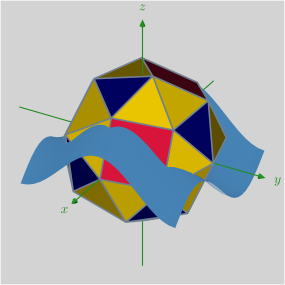
\includegraphics[height=7.5cm]{polyedre.png}%
\else% TeXgraph version 1.989
\bgroup%
%\shorthandoff{;:!?}% uncomment if problem with babel
\pgfdeclarehorizontalshading[colorA,colorB]{myshading}{100bp}{color(0bp)=(colorA);color(75bp)=(colorB)}%
\pgfdeclareradialshading[colorA,colorB]{mysphereshading}{\pgfpoint{\GradCenterX bp}{\GradCenterY bp}}{color(0bp)=(colorA); color(35bp)=(colorB)}%
%\shorthandon{;:!?}% uncomment if problem with babel
\begin{tikzpicture}%
\pgfsetxvec{\pgfxy(0.75,0)}%
\pgfsetyvec{\pgfxy(0,0.75)}%
\useasboundingbox (-5,-5)--(5,5);
%objet1  (User)
\pgfsetstrokecolor{rgb,1:red,0;green,0;blue,0}%
\pgfsetlinewidth{0.4pt}%
\pgfsetroundjoin%
\pgfpathmoveto{\pgfxy(-5,5)}%
\pgfpathlineto{\pgfxy(-5,-5)}\pgfpathlineto{\pgfxy(5,-5)}\pgfpathlineto{\pgfxy(5,5)}\pgfclosepath%
\pgfsetfillcolor{rgb,1:red,0.8275;green,0.8275;blue,0.8275}%
\pgffill%
\pgfsetstrokecolor{rgb,1:red,0.2353;green,0.4392;blue,0.6118}%
\pgfsetlinewidth{0.2pt}%
\pgfpathmoveto{\pgfxy(2.6599,-1.6768)}%
\pgfpathlineto{\pgfxy(2.529,-1.6108)}\pgfpathlineto{\pgfxy(2.7558,-1.7628)}\pgfpathlineto{\pgfxy(2.8867,-1.8287)}\pgfclosepath%
\pgfsetfillcolor{rgb,1:red,0.2353;green,0.4392;blue,0.6118}%
\pgffillstroke%
\pgfsetstrokecolor{rgb,1:red,0.2745;green,0.5098;blue,0.7059}%
\pgfpathmoveto{\pgfxy(3.0298,0.3371)}%
\pgfpathlineto{\pgfxy(3.2537,0.0662)}\pgfpathlineto{\pgfxy(3.3846,0.4037)}\pgfpathlineto{\pgfxy(3.1865,0.6435)}\pgfclosepath%
\pgfsetfillcolor{rgb,1:red,0.2745;green,0.5098;blue,0.7059}%
\pgffillstroke%
\pgfpathmoveto{\pgfxy(3.3846,0.4037)}%
\pgfpathlineto{\pgfxy(3.2537,0.0662)}\pgfpathlineto{\pgfxy(3.4804,-0.1786)}\pgfpathlineto{\pgfxy(3.6113,0.1589)}\pgfclosepath%
\pgfsetfillcolor{rgb,1:red,0.2745;green,0.5098;blue,0.7059}%
\pgffillstroke%
\pgfpathmoveto{\pgfxy(3.4804,-0.1786)}%
\pgfpathlineto{\pgfxy(3.3495,-0.5008)}\pgfpathlineto{\pgfxy(3.5762,-0.7039)}\pgfpathlineto{\pgfxy(3.7071,-0.3817)}\pgfclosepath%
\pgfsetfillcolor{rgb,1:red,0.2745;green,0.5098;blue,0.7059}%
\pgffillstroke%
\pgfpathmoveto{\pgfxy(3.6113,0.1589)}%
\pgfpathlineto{\pgfxy(3.4804,-0.1786)}\pgfpathlineto{\pgfxy(3.7071,-0.3817)}\pgfpathlineto{\pgfxy(3.838,-0.0441)}\pgfclosepath%
\pgfsetfillcolor{rgb,1:red,0.2745;green,0.5098;blue,0.7059}%
\pgffillstroke%
\pgfpathmoveto{\pgfxy(3.009,0.2963)}%
\pgfpathlineto{\pgfxy(2.8961,0.0183)}\pgfpathlineto{\pgfxy(3.1228,-0.256)}\pgfpathlineto{\pgfxy(3.2537,0.0662)}\pgfpathlineto{\pgfxy(3.0298,0.3371)}%
\pgfclosepath%
\pgfsetfillcolor{rgb,1:red,0.2745;green,0.5098;blue,0.7059}%
\pgffillstroke%
\pgfpathmoveto{\pgfxy(3.2537,0.0662)}%
\pgfpathlineto{\pgfxy(3.1228,-0.256)}\pgfpathlineto{\pgfxy(3.3495,-0.5008)}\pgfpathlineto{\pgfxy(3.4804,-0.1786)}\pgfclosepath%
\pgfsetfillcolor{rgb,1:red,0.2745;green,0.5098;blue,0.7059}%
\pgffillstroke%
\pgfpathmoveto{\pgfxy(3.838,-0.0441)}%
\pgfpathlineto{\pgfxy(3.7071,-0.3817)}\pgfpathlineto{\pgfxy(3.9339,-0.5336)}\pgfpathlineto{\pgfxy(4.0648,-0.1961)}\pgfclosepath%
\pgfsetfillcolor{rgb,1:red,0.2745;green,0.5098;blue,0.7059}%
\pgffillstroke%
\pgfpathmoveto{\pgfxy(2.8785,0.0408)}%
\pgfpathlineto{\pgfxy(2.8961,0.0183)}\pgfpathlineto{\pgfxy(3.009,0.2963)}\pgfclosepath%
\pgfsetfillcolor{rgb,1:red,0.2745;green,0.5098;blue,0.7059}%
\pgffillstroke%
\pgfpathmoveto{\pgfxy(2.8961,0.0183)}%
\pgfpathlineto{\pgfxy(2.7652,-0.2744)}\pgfpathlineto{\pgfxy(2.9919,-0.5487)}\pgfpathlineto{\pgfxy(3.1228,-0.256)}\pgfclosepath%
\pgfsetfillcolor{rgb,1:red,0.2745;green,0.5098;blue,0.7059}%
\pgffillstroke%
\pgfpathmoveto{\pgfxy(3.7071,-0.3817)}%
\pgfpathlineto{\pgfxy(3.5762,-0.7039)}\pgfpathlineto{\pgfxy(3.803,-0.8559)}\pgfpathlineto{\pgfxy(3.9339,-0.5336)}\pgfclosepath%
\pgfsetfillcolor{rgb,1:red,0.2745;green,0.5098;blue,0.7059}%
\pgffillstroke%
\pgfsetstrokecolor{rgb,1:red,0.2745;green,0.5059;blue,0.702}%
\pgfpathmoveto{\pgfxy(4.0648,-0.1961)}%
\pgfpathlineto{\pgfxy(3.9339,-0.5336)}\pgfpathlineto{\pgfxy(4.1606,-0.6286)}\pgfpathlineto{\pgfxy(4.2915,-0.2911)}\pgfclosepath%
\pgfsetfillcolor{rgb,1:red,0.2745;green,0.5059;blue,0.702}%
\pgffillstroke%
\pgfsetstrokecolor{rgb,1:red,0.2745;green,0.5098;blue,0.7059}%
\pgfpathmoveto{\pgfxy(3.1228,-0.256)}%
\pgfpathlineto{\pgfxy(2.9919,-0.5487)}\pgfpathlineto{\pgfxy(3.2186,-0.7935)}\pgfpathlineto{\pgfxy(3.3495,-0.5008)}\pgfclosepath%
\pgfsetfillcolor{rgb,1:red,0.2745;green,0.5098;blue,0.7059}%
\pgffillstroke%
\pgfsetstrokecolor{rgb,1:red,0.2745;green,0.5098;blue,0.702}%
\pgfpathmoveto{\pgfxy(2.7363,-0.2376)}%
\pgfpathlineto{\pgfxy(2.7652,-0.2744)}\pgfpathlineto{\pgfxy(2.8961,0.0183)}\pgfpathlineto{\pgfxy(2.8785,0.0408)}\pgfclosepath%
\pgfsetfillcolor{rgb,1:red,0.2745;green,0.5098;blue,0.702}%
\pgffillstroke%
\pgfsetstrokecolor{rgb,1:red,0.2745;green,0.5098;blue,0.7059}%
\pgfpathmoveto{\pgfxy(3.3495,-0.5008)}%
\pgfpathlineto{\pgfxy(3.2186,-0.7935)}\pgfpathlineto{\pgfxy(3.4453,-0.9966)}\pgfpathlineto{\pgfxy(3.5762,-0.7039)}\pgfclosepath%
\pgfsetfillcolor{rgb,1:red,0.2745;green,0.5098;blue,0.7059}%
\pgffillstroke%
\pgfsetstrokecolor{rgb,1:red,0.2745;green,0.5059;blue,0.702}%
\pgfpathmoveto{\pgfxy(3.803,-0.8559)}%
\pgfpathlineto{\pgfxy(3.6721,-1.1486)}\pgfpathlineto{\pgfxy(3.8988,-1.2435)}\pgfpathlineto{\pgfxy(4.0297,-0.9508)}\pgfclosepath%
\pgfsetfillcolor{rgb,1:red,0.2745;green,0.5059;blue,0.702}%
\pgffillstroke%
\pgfpathmoveto{\pgfxy(3.9339,-0.5336)}%
\pgfpathlineto{\pgfxy(3.803,-0.8559)}\pgfpathlineto{\pgfxy(4.0297,-0.9508)}\pgfpathlineto{\pgfxy(4.1606,-0.6286)}\pgfclosepath%
\pgfsetfillcolor{rgb,1:red,0.2745;green,0.5059;blue,0.702}%
\pgffillstroke%
\pgfsetstrokecolor{rgb,1:red,0.2745;green,0.5098;blue,0.702}%
\pgfpathmoveto{\pgfxy(3.5762,-0.7039)}%
\pgfpathlineto{\pgfxy(3.4453,-0.9966)}\pgfpathlineto{\pgfxy(3.6721,-1.1486)}\pgfpathlineto{\pgfxy(3.803,-0.8559)}\pgfclosepath%
\pgfsetfillcolor{rgb,1:red,0.2745;green,0.5098;blue,0.702}%
\pgffillstroke%
\pgfsetstrokecolor{rgb,1:red,0.2745;green,0.5059;blue,0.702}%
\pgfpathmoveto{\pgfxy(2.7652,-0.2744)}%
\pgfpathlineto{\pgfxy(2.6343,-0.5254)}\pgfpathlineto{\pgfxy(2.861,-0.7997)}\pgfpathlineto{\pgfxy(2.9919,-0.5487)}\pgfclosepath%
\pgfsetfillcolor{rgb,1:red,0.2745;green,0.5059;blue,0.702}%
\pgffillstroke%
\pgfpathmoveto{\pgfxy(2.6072,-0.4909)}%
\pgfpathlineto{\pgfxy(2.6343,-0.5254)}\pgfpathlineto{\pgfxy(2.7652,-0.2744)}\pgfpathlineto{\pgfxy(2.7363,-0.2376)}\pgfclosepath%
\pgfsetfillcolor{rgb,1:red,0.2745;green,0.5059;blue,0.702}%
\pgffillstroke%
\pgfpathmoveto{\pgfxy(2.9919,-0.5487)}%
\pgfpathlineto{\pgfxy(2.861,-0.7997)}\pgfpathlineto{\pgfxy(3.0877,-1.0445)}\pgfpathlineto{\pgfxy(3.2186,-0.7935)}\pgfclosepath%
\pgfsetfillcolor{rgb,1:red,0.2745;green,0.5059;blue,0.702}%
\pgffillstroke%
\pgfpathmoveto{\pgfxy(3.2186,-0.7935)}%
\pgfpathlineto{\pgfxy(3.0877,-1.0445)}\pgfpathlineto{\pgfxy(3.3144,-1.2476)}\pgfpathlineto{\pgfxy(3.4453,-0.9966)}\pgfclosepath%
\pgfsetfillcolor{rgb,1:red,0.2745;green,0.5059;blue,0.702}%
\pgffillstroke%
\pgfsetstrokecolor{rgb,1:red,0.2706;green,0.5059;blue,0.698}%
\pgfpathmoveto{\pgfxy(2.6343,-0.5254)}%
\pgfpathlineto{\pgfxy(2.5034,-0.7253)}\pgfpathlineto{\pgfxy(2.7301,-0.9996)}\pgfpathlineto{\pgfxy(2.861,-0.7997)}\pgfclosepath%
\pgfsetfillcolor{rgb,1:red,0.2706;green,0.5059;blue,0.698}%
\pgffillstroke%
\pgfsetstrokecolor{rgb,1:red,0.2745;green,0.5059;blue,0.702}%
\pgfpathmoveto{\pgfxy(3.4453,-0.9966)}%
\pgfpathlineto{\pgfxy(3.3144,-1.2476)}\pgfpathlineto{\pgfxy(3.5412,-1.3996)}\pgfpathlineto{\pgfxy(3.6721,-1.1486)}\pgfclosepath%
\pgfsetfillcolor{rgb,1:red,0.2745;green,0.5059;blue,0.702}%
\pgffillstroke%
\pgfsetstrokecolor{rgb,1:red,0.2706;green,0.5059;blue,0.702}%
\pgfpathmoveto{\pgfxy(3.6721,-1.1486)}%
\pgfpathlineto{\pgfxy(3.5412,-1.3996)}\pgfpathlineto{\pgfxy(3.7679,-1.4945)}\pgfpathlineto{\pgfxy(3.8988,-1.2435)}\pgfclosepath%
\pgfsetfillcolor{rgb,1:red,0.2706;green,0.5059;blue,0.702}%
\pgffillstroke%
\pgfsetstrokecolor{rgb,1:red,0.2706;green,0.5059;blue,0.698}%
\pgfpathmoveto{\pgfxy(2.494,-0.7134)}%
\pgfpathlineto{\pgfxy(2.5034,-0.7253)}\pgfpathlineto{\pgfxy(2.6343,-0.5254)}\pgfpathlineto{\pgfxy(2.6072,-0.4909)}\pgfclosepath%
\pgfsetfillcolor{rgb,1:red,0.2706;green,0.5059;blue,0.698}%
\pgffillstroke%
\pgfsetstrokecolor{rgb,1:red,0.2706;green,0.5059;blue,0.702}%
\pgfpathmoveto{\pgfxy(2.861,-0.7997)}%
\pgfpathlineto{\pgfxy(2.7301,-0.9996)}\pgfpathlineto{\pgfxy(2.9568,-1.2444)}\pgfpathlineto{\pgfxy(3.0877,-1.0445)}\pgfclosepath%
\pgfsetfillcolor{rgb,1:red,0.2706;green,0.5059;blue,0.702}%
\pgffillstroke%
\pgfpathmoveto{\pgfxy(3.0877,-1.0445)}%
\pgfpathlineto{\pgfxy(2.9568,-1.2444)}\pgfpathlineto{\pgfxy(3.1835,-1.4475)}\pgfpathlineto{\pgfxy(3.3144,-1.2476)}\pgfclosepath%
\pgfsetfillcolor{rgb,1:red,0.2706;green,0.5059;blue,0.702}%
\pgffillstroke%
\pgfsetstrokecolor{rgb,1:red,0.2706;green,0.5059;blue,0.698}%
\pgfpathmoveto{\pgfxy(3.3144,-1.2476)}%
\pgfpathlineto{\pgfxy(3.1835,-1.4475)}\pgfpathlineto{\pgfxy(3.4103,-1.5994)}\pgfpathlineto{\pgfxy(3.5412,-1.3996)}\pgfclosepath%
\pgfsetfillcolor{rgb,1:red,0.2706;green,0.5059;blue,0.698}%
\pgffillstroke%
\pgfsetstrokecolor{rgb,1:red,0.2706;green,0.502;blue,0.698}%
\pgfpathmoveto{\pgfxy(3.5412,-1.3996)}%
\pgfpathlineto{\pgfxy(3.4103,-1.5994)}\pgfpathlineto{\pgfxy(3.637,-1.6944)}\pgfpathlineto{\pgfxy(3.7679,-1.4945)}\pgfclosepath%
\pgfsetfillcolor{rgb,1:red,0.2706;green,0.502;blue,0.698}%
\pgffillstroke%
\pgfsetstrokecolor{rgb,1:red,0.2706;green,0.502;blue,0.6941}%
\pgfpathmoveto{\pgfxy(2.469,-0.7628)}%
\pgfpathlineto{\pgfxy(2.5034,-0.7253)}\pgfpathlineto{\pgfxy(2.494,-0.7134)}\pgfclosepath%
\pgfsetfillcolor{rgb,1:red,0.2706;green,0.502;blue,0.6941}%
\pgffillstroke%
\pgfpathmoveto{\pgfxy(2.7301,-0.9996)}%
\pgfpathlineto{\pgfxy(2.5992,-1.1425)}\pgfpathlineto{\pgfxy(2.8259,-1.3873)}\pgfpathlineto{\pgfxy(2.9568,-1.2444)}\pgfclosepath%
\pgfsetfillcolor{rgb,1:red,0.2706;green,0.502;blue,0.6941}%
\pgffillstroke%
\pgfpathmoveto{\pgfxy(2.5034,-0.7253)}%
\pgfpathlineto{\pgfxy(2.469,-0.7628)}\pgfpathlineto{\pgfxy(2.3992,-0.9005)}\pgfpathlineto{\pgfxy(2.5992,-1.1425)}\pgfpathlineto{\pgfxy(2.7301,-0.9996)}%
\pgfclosepath%
\pgfsetfillcolor{rgb,1:red,0.2706;green,0.502;blue,0.6941}%
\pgffillstroke%
\pgfpathmoveto{\pgfxy(2.9568,-1.2444)}%
\pgfpathlineto{\pgfxy(2.8259,-1.3873)}\pgfpathlineto{\pgfxy(3.0526,-1.5903)}\pgfpathlineto{\pgfxy(3.1835,-1.4475)}\pgfclosepath%
\pgfsetfillcolor{rgb,1:red,0.2706;green,0.502;blue,0.6941}%
\pgffillstroke%
\pgfsetstrokecolor{rgb,1:red,0.2667;green,0.498;blue,0.6902}%
\pgfpathmoveto{\pgfxy(3.4103,-1.5994)}%
\pgfpathlineto{\pgfxy(3.2794,-1.7423)}\pgfpathlineto{\pgfxy(3.5061,-1.8373)}\pgfpathlineto{\pgfxy(3.637,-1.6944)}\pgfclosepath%
\pgfsetfillcolor{rgb,1:red,0.2667;green,0.498;blue,0.6902}%
\pgffillstroke%
\pgfsetstrokecolor{rgb,1:red,0.2706;green,0.502;blue,0.6941}%
\pgfpathmoveto{\pgfxy(3.1835,-1.4475)}%
\pgfpathlineto{\pgfxy(3.0526,-1.5903)}\pgfpathlineto{\pgfxy(3.2794,-1.7423)}\pgfpathlineto{\pgfxy(3.4103,-1.5994)}\pgfclosepath%
\pgfsetfillcolor{rgb,1:red,0.2706;green,0.502;blue,0.6941}%
\pgffillstroke%
\pgfsetstrokecolor{rgb,1:red,0.2667;green,0.498;blue,0.6863}%
\pgfpathmoveto{\pgfxy(2.3233,-1.0509)}%
\pgfpathlineto{\pgfxy(2.4683,-1.2263)}\pgfpathlineto{\pgfxy(2.5992,-1.1425)}\pgfpathlineto{\pgfxy(2.3992,-0.9005)}\pgfclosepath%
\pgfsetfillcolor{rgb,1:red,0.2667;green,0.498;blue,0.6863}%
\pgffillstroke%
\pgfpathmoveto{\pgfxy(2.5992,-1.1425)}%
\pgfpathlineto{\pgfxy(2.4683,-1.2263)}\pgfpathlineto{\pgfxy(2.695,-1.4711)}\pgfpathlineto{\pgfxy(2.8259,-1.3873)}\pgfclosepath%
\pgfsetfillcolor{rgb,1:red,0.2667;green,0.498;blue,0.6863}%
\pgffillstroke%
\pgfsetstrokecolor{rgb,1:red,0.2667;green,0.4941;blue,0.6863}%
\pgfpathmoveto{\pgfxy(2.8259,-1.3873)}%
\pgfpathlineto{\pgfxy(2.695,-1.4711)}\pgfpathlineto{\pgfxy(2.9217,-1.6742)}\pgfpathlineto{\pgfxy(3.0526,-1.5903)}\pgfclosepath%
\pgfsetfillcolor{rgb,1:red,0.2667;green,0.4941;blue,0.6863}%
\pgffillstroke%
\pgfsetstrokecolor{rgb,1:red,0.2667;green,0.4941;blue,0.6824}%
\pgfpathmoveto{\pgfxy(3.0526,-1.5903)}%
\pgfpathlineto{\pgfxy(2.9217,-1.6742)}\pgfpathlineto{\pgfxy(3.1485,-1.8262)}\pgfpathlineto{\pgfxy(3.2794,-1.7423)}\pgfclosepath%
\pgfsetfillcolor{rgb,1:red,0.2667;green,0.4941;blue,0.6824}%
\pgffillstroke%
\pgfsetstrokecolor{rgb,1:red,0.2627;green,0.4902;blue,0.6784}%
\pgfpathmoveto{\pgfxy(3.2794,-1.7423)}%
\pgfpathlineto{\pgfxy(3.1485,-1.8262)}\pgfpathlineto{\pgfxy(3.3752,-1.9211)}\pgfpathlineto{\pgfxy(3.5061,-1.8373)}\pgfclosepath%
\pgfsetfillcolor{rgb,1:red,0.2627;green,0.4902;blue,0.6784}%
\pgffillstroke%
\pgfpathmoveto{\pgfxy(2.2656,-1.1663)}%
\pgfpathlineto{\pgfxy(2.3374,-1.2532)}\pgfpathlineto{\pgfxy(2.4683,-1.2263)}\pgfpathlineto{\pgfxy(2.3233,-1.0509)}\pgfclosepath%
\pgfsetfillcolor{rgb,1:red,0.2627;green,0.4902;blue,0.6784}%
\pgffillstroke%
\pgfsetstrokecolor{rgb,1:red,0.2627;green,0.4863;blue,0.6745}%
\pgfpathmoveto{\pgfxy(2.4683,-1.2263)}%
\pgfpathlineto{\pgfxy(2.3374,-1.2532)}\pgfpathlineto{\pgfxy(2.5641,-1.498)}\pgfpathlineto{\pgfxy(2.695,-1.4711)}\pgfclosepath%
\pgfsetfillcolor{rgb,1:red,0.2627;green,0.4863;blue,0.6745}%
\pgffillstroke%
\pgfpathmoveto{\pgfxy(2.695,-1.4711)}%
\pgfpathlineto{\pgfxy(2.5641,-1.498)}\pgfpathlineto{\pgfxy(2.7908,-1.701)}\pgfpathlineto{\pgfxy(2.9217,-1.6742)}\pgfclosepath%
\pgfsetfillcolor{rgb,1:red,0.2627;green,0.4863;blue,0.6745}%
\pgffillstroke%
\pgfsetstrokecolor{rgb,1:red,0.2588;green,0.4824;blue,0.6667}%
\pgfpathmoveto{\pgfxy(2.9217,-1.6742)}%
\pgfpathlineto{\pgfxy(2.7908,-1.701)}\pgfpathlineto{\pgfxy(3.0176,-1.853)}\pgfpathlineto{\pgfxy(3.1485,-1.8262)}\pgfclosepath%
\pgfsetfillcolor{rgb,1:red,0.2588;green,0.4824;blue,0.6667}%
\pgffillstroke%
\pgfsetstrokecolor{rgb,1:red,0.2549;green,0.4745;blue,0.6588}%
\pgfpathmoveto{\pgfxy(3.1485,-1.8262)}%
\pgfpathlineto{\pgfxy(3.0176,-1.853)}\pgfpathlineto{\pgfxy(3.2443,-1.948)}\pgfpathlineto{\pgfxy(3.3752,-1.9211)}\pgfclosepath%
\pgfsetfillcolor{rgb,1:red,0.2549;green,0.4745;blue,0.6588}%
\pgffillstroke%
\pgfsetstrokecolor{rgb,1:red,0.2588;green,0.4784;blue,0.6627}%
\pgfpathmoveto{\pgfxy(2.3374,-1.2532)}%
\pgfpathlineto{\pgfxy(2.2323,-1.2337)}\pgfpathlineto{\pgfxy(2.2249,-1.2488)}\pgfpathlineto{\pgfxy(2.4332,-1.4737)}\pgfpathlineto{\pgfxy(2.5641,-1.498)}%
\pgfclosepath%
\pgfsetfillcolor{rgb,1:red,0.2588;green,0.4784;blue,0.6627}%
\pgffillstroke%
\pgfpathmoveto{\pgfxy(2.2323,-1.2337)}%
\pgfpathlineto{\pgfxy(2.3374,-1.2532)}\pgfpathlineto{\pgfxy(2.2656,-1.1663)}\pgfclosepath%
\pgfsetfillcolor{rgb,1:red,0.2588;green,0.4784;blue,0.6627}%
\pgffillstroke%
\pgfsetstrokecolor{rgb,1:red,0.2549;green,0.4745;blue,0.6549}%
\pgfpathmoveto{\pgfxy(2.5641,-1.498)}%
\pgfpathlineto{\pgfxy(2.4332,-1.4737)}\pgfpathlineto{\pgfxy(2.6599,-1.6768)}\pgfpathlineto{\pgfxy(2.7908,-1.701)}\pgfclosepath%
\pgfsetfillcolor{rgb,1:red,0.2549;green,0.4745;blue,0.6549}%
\pgffillstroke%
\pgfsetstrokecolor{rgb,1:red,0.251;green,0.4667;blue,0.6471}%
\pgfpathmoveto{\pgfxy(2.7908,-1.701)}%
\pgfpathlineto{\pgfxy(2.6599,-1.6768)}\pgfpathlineto{\pgfxy(2.8867,-1.8287)}\pgfpathlineto{\pgfxy(3.0176,-1.853)}\pgfclosepath%
\pgfsetfillcolor{rgb,1:red,0.251;green,0.4667;blue,0.6471}%
\pgffillstroke%
\pgfsetstrokecolor{rgb,1:red,0.2431;green,0.451;blue,0.6235}%
\pgfpathmoveto{\pgfxy(3.0176,-1.853)}%
\pgfpathlineto{\pgfxy(2.8867,-1.8287)}\pgfpathlineto{\pgfxy(3.1134,-1.9237)}\pgfpathlineto{\pgfxy(3.2443,-1.948)}\pgfclosepath%
\pgfsetfillcolor{rgb,1:red,0.2431;green,0.451;blue,0.6235}%
\pgffillstroke%
\pgfsetstrokecolor{rgb,1:red,0.251;green,0.4667;blue,0.6471}%
\pgfpathmoveto{\pgfxy(2.2012,-1.2985)}%
\pgfpathlineto{\pgfxy(2.3023,-1.4077)}\pgfpathlineto{\pgfxy(2.4332,-1.4737)}\pgfpathlineto{\pgfxy(2.2249,-1.2488)}\pgfclosepath%
\pgfsetfillcolor{rgb,1:red,0.251;green,0.4667;blue,0.6471}%
\pgffillstroke%
\pgfsetstrokecolor{rgb,1:red,0.2471;green,0.4588;blue,0.6353}%
\pgfpathmoveto{\pgfxy(2.4332,-1.4737)}%
\pgfpathlineto{\pgfxy(2.3023,-1.4077)}\pgfpathlineto{\pgfxy(2.529,-1.6108)}\pgfpathlineto{\pgfxy(2.6599,-1.6768)}\pgfclosepath%
\pgfsetfillcolor{rgb,1:red,0.2471;green,0.4588;blue,0.6353}%
\pgffillstroke%
\pgfsetstrokecolor{rgb,1:red,0.2431;green,0.4549;blue,0.6275}%
\pgfpathmoveto{\pgfxy(2.1892,-1.3251)}%
\pgfpathlineto{\pgfxy(2.3023,-1.4077)}\pgfpathlineto{\pgfxy(2.2012,-1.2985)}\pgfclosepath%
\pgfsetfillcolor{rgb,1:red,0.2431;green,0.4549;blue,0.6275}%
\pgffillstroke%
\pgfsetstrokecolor{rgb,1:red,0.2353;green,0.4392;blue,0.6078}%
\pgfpathmoveto{\pgfxy(2.3023,-1.4077)}%
\pgfpathlineto{\pgfxy(2.1883,-1.3273)}\pgfpathlineto{\pgfxy(2.3981,-1.5153)}\pgfpathlineto{\pgfxy(2.529,-1.6108)}\pgfclosepath%
\pgfsetfillcolor{rgb,1:red,0.2353;green,0.4392;blue,0.6078}%
\pgffillstroke%
\pgfsetstrokecolor{rgb,1:red,0.2235;green,0.4118;blue,0.5686}%
\pgfpathmoveto{\pgfxy(2.1874,-1.333)}%
\pgfpathlineto{\pgfxy(2.2672,-1.4045)}\pgfpathlineto{\pgfxy(2.3981,-1.5153)}\pgfpathlineto{\pgfxy(2.1883,-1.3273)}\pgfclosepath%
\pgfsetfillcolor{rgb,1:red,0.2235;green,0.4118;blue,0.5686}%
\pgffillstroke%
\pgfpathmoveto{\pgfxy(2.1869,-1.3365)}%
\pgfpathlineto{\pgfxy(2.2672,-1.4045)}\pgfpathlineto{\pgfxy(2.1874,-1.333)}\pgfclosepath%
\pgfsetfillcolor{rgb,1:red,0.2235;green,0.4118;blue,0.5686}%
\pgffillstroke%
\pgfsetstrokecolor{rgb,1:red,0.5647;green,0.7686;blue,0.5647}%
\pgfsetlinewidth{0.1pt}%
\pgfpathmoveto{\pgfxy(4.1291,-1.2565)}%
\pgfpathlineto{\pgfxy(4.1541,-1.2034)}\pgfpathlineto{\pgfxy(4.3301,-1.25)}\pgfclosepath%
\pgfsetfillcolor{rgb,1:red,0.6314;green,0.8627;blue,0.6314}%
\pgffillstroke%
\pgfpathmoveto{\pgfxy(4.1541,-1.2034)}%
\pgfpathlineto{\pgfxy(4.1636,-1.1442)}\pgfpathlineto{\pgfxy(4.3301,-1.25)}\pgfclosepath%
\pgfsetfillcolor{rgb,1:red,0.5922;green,0.8039;blue,0.5922}%
\pgffillstroke%
\pgfpathmoveto{\pgfxy(4.1636,-1.1442)}%
\pgfpathlineto{\pgfxy(4.1541,-1.1016)}\pgfpathlineto{\pgfxy(4.3301,-1.25)}\pgfclosepath%
\pgfsetfillcolor{rgb,1:red,0.4314;green,0.5882;blue,0.4314}%
\pgffillstroke%
\pgfpathmoveto{\pgfxy(4.0982,-1.2832)}%
\pgfpathlineto{\pgfxy(4.1291,-1.2565)}\pgfpathlineto{\pgfxy(4.3301,-1.25)}\pgfclosepath%
\pgfsetfillcolor{rgb,1:red,0.5843;green,0.7961;blue,0.5843}%
\pgffillstroke%
\pgfsetstrokecolor{rgb,1:red,0.1333;green,0.5451;blue,0.1333}%
\pgfsetlinewidth{0.8pt}%
\pgfsetroundcap%
\pgfxyline(4.1136,-1.1875)(2.5034,-0.7227)%
\pgfsetlinewidth{0.1pt}%
\pgfpathmoveto{\pgfxy(4.0732,-1.1716)}%
\pgfpathlineto{\pgfxy(4.0636,-1.2308)}\pgfpathlineto{\pgfxy(4.3301,-1.25)}\pgfclosepath%
\pgfsetfillcolor{rgb,1:red,0.1412;green,0.5725;blue,0.1412}%
\pgffillstroke%
\pgfpathmoveto{\pgfxy(4.0982,-1.1185)}%
\pgfpathlineto{\pgfxy(4.0732,-1.1716)}\pgfpathlineto{\pgfxy(4.3301,-1.25)}\pgfclosepath%
\pgfsetfillcolor{rgb,1:red,0.149;green,0.6157;blue,0.149}%
\pgffillstroke%
\pgfpathmoveto{\pgfxy(4.1291,-1.0918)}%
\pgfpathlineto{\pgfxy(4.0982,-1.1185)}\pgfpathlineto{\pgfxy(4.3301,-1.25)}\pgfclosepath%
\pgfsetfillcolor{rgb,1:red,0.1373;green,0.5686;blue,0.1373}%
\pgffillstroke%
\pgfpathmoveto{\pgfxy(4.0732,-1.2734)}%
\pgfpathlineto{\pgfxy(4.0982,-1.2832)}\pgfpathlineto{\pgfxy(4.3301,-1.25)}\pgfclosepath%
\pgfsetfillcolor{rgb,1:red,0.098;green,0.4039;blue,0.098}%
\pgffillstroke%
\pgfpathmoveto{\pgfxy(4.0636,-1.2308)}%
\pgfpathlineto{\pgfxy(4.0732,-1.2734)}\pgfpathlineto{\pgfxy(4.3301,-1.25)}\pgfclosepath%
\pgfsetfillcolor{rgb,1:red,0.102;green,0.4235;blue,0.102}%
\pgffillstroke%
\pgfpathmoveto{\pgfxy(4.1541,-1.1016)}%
\pgfpathlineto{\pgfxy(4.1291,-1.0918)}\pgfpathlineto{\pgfxy(4.3301,-1.25)}\pgfclosepath%
\pgfsetfillcolor{rgb,1:red,0.102;green,0.4078;blue,0.102}%
\pgffillstroke%
\pgfsetlinewidth{0.3pt}%
\pgfputat{\pgfxy(4.7631,-1.375)}{\pgftext{\color{rgb,1:red,0.1333;green,0.5451;blue,0.1333}\small $y$}}\pgfstroke%
\pgfsetstrokecolor{rgb,1:red,0.5725;green,0.6784;blue,0.7686}%
\pgfsetlinewidth{0.2pt}%
\pgfpathmoveto{\pgfxy(2.494,-1.5565)}%
\pgfpathlineto{\pgfxy(2.3631,-1.4457)}\pgfpathlineto{\pgfxy(2.5898,-1.5406)}\pgfpathlineto{\pgfxy(2.7207,-1.6514)}\pgfclosepath%
\pgfsetfillcolor{rgb,1:red,0.5725;green,0.6784;blue,0.7686}%
\pgffillstroke%
\pgfsetstrokecolor{rgb,1:red,0.549;green,0.651;blue,0.7333}%
\pgfpathmoveto{\pgfxy(2.2672,-1.4045)}%
\pgfpathlineto{\pgfxy(2.1869,-1.3365)}\pgfpathlineto{\pgfxy(2.1909,-1.3302)}\pgfpathlineto{\pgfxy(2.3631,-1.4457)}\pgfpathlineto{\pgfxy(2.494,-1.5565)}%
\pgfclosepath%
\pgfsetfillcolor{rgb,1:red,0.549;green,0.651;blue,0.7333}%
\pgffillstroke%
\pgfpathmoveto{\pgfxy(2.3981,-1.5153)}%
\pgfpathlineto{\pgfxy(2.2672,-1.4045)}\pgfpathlineto{\pgfxy(2.494,-1.5565)}\pgfpathlineto{\pgfxy(2.6249,-1.6672)}\pgfclosepath%
\pgfsetfillcolor{rgb,1:red,0.549;green,0.651;blue,0.7333}%
\pgffillstroke%
\pgfsetstrokecolor{rgb,1:red,0.5216;green,0.6157;blue,0.698}%
\pgfpathmoveto{\pgfxy(2.3631,-1.4457)}%
\pgfpathlineto{\pgfxy(2.1909,-1.3302)}\pgfpathlineto{\pgfxy(2.1948,-1.3261)}\pgfclosepath%
\pgfsetfillcolor{rgb,1:red,0.5216;green,0.6157;blue,0.698}%
\pgffillstroke%
\pgfsetstrokecolor{rgb,1:red,0.5725;green,0.6784;blue,0.7686}%
\pgfpathmoveto{\pgfxy(2.6249,-1.6672)}%
\pgfpathlineto{\pgfxy(2.494,-1.5565)}\pgfpathlineto{\pgfxy(2.7207,-1.6514)}\pgfpathlineto{\pgfxy(2.8516,-1.7622)}\pgfclosepath%
\pgfsetfillcolor{rgb,1:red,0.5725;green,0.6784;blue,0.7686}%
\pgffillstroke%
\pgfsetstrokecolor{rgb,1:red,0.5647;green,0.6706;blue,0.7569}%
\pgfpathmoveto{\pgfxy(2.3631,-1.4457)}%
\pgfpathlineto{\pgfxy(2.2322,-1.3502)}\pgfpathlineto{\pgfxy(2.4589,-1.4451)}\pgfpathlineto{\pgfxy(2.5898,-1.5406)}\pgfclosepath%
\pgfsetfillcolor{rgb,1:red,0.5647;green,0.6706;blue,0.7569}%
\pgffillstroke%
\pgfsetstrokecolor{rgb,1:red,0.5333;green,0.6314;blue,0.7137}%
\pgfpathmoveto{\pgfxy(2.2322,-1.3502)}%
\pgfpathlineto{\pgfxy(2.2186,-1.3333)}\pgfpathlineto{\pgfxy(2.328,-1.3791)}\pgfpathlineto{\pgfxy(2.4589,-1.4451)}\pgfclosepath%
\pgfsetfillcolor{rgb,1:red,0.5333;green,0.6314;blue,0.7137}%
\pgffillstroke%
\pgfsetstrokecolor{rgb,1:red,0.2431;green,0.451;blue,0.6235}%
\pgfpathmoveto{\pgfxy(2.328,-1.3791)}%
\pgfpathlineto{\pgfxy(2.2209,-1.3347)}\pgfclosepath%
\pgfsetfillcolor{rgb,1:red,0.2431;green,0.451;blue,0.6235}%
\pgffillstroke%
\pgfsetstrokecolor{rgb,1:red,0.5216;green,0.6157;blue,0.698}%
\pgfpathmoveto{\pgfxy(2.1953,-1.3255)}%
\pgfpathlineto{\pgfxy(2.2322,-1.3502)}\pgfpathlineto{\pgfxy(2.3631,-1.4457)}\pgfclosepath%
\pgfsetfillcolor{rgb,1:red,0.5216;green,0.6157;blue,0.698}%
\pgffillstroke%
\pgfsetstrokecolor{rgb,1:red,0.2353;green,0.4392;blue,0.6118}%
\pgfpathmoveto{\pgfxy(2.1933,-1.3306)}%
\pgfpathlineto{\pgfxy(2.2322,-1.3502)}\pgfpathlineto{\pgfxy(2.1953,-1.3255)}\pgfclosepath%
\pgfsetfillcolor{rgb,1:red,0.2353;green,0.4392;blue,0.6118}%
\pgffillstroke%
\pgfsetstrokecolor{rgb,1:red,0.5333;green,0.6314;blue,0.7137}%
\pgfpathmoveto{\pgfxy(2.2322,-1.3502)}%
\pgfpathlineto{\pgfxy(2.1933,-1.3306)}\pgfpathlineto{\pgfxy(2.1978,-1.3246)}\pgfpathlineto{\pgfxy(2.2186,-1.3333)}\pgfclosepath%
\pgfsetfillcolor{rgb,1:red,0.5333;green,0.6314;blue,0.7137}%
\pgffillstroke%
\pgfsetstrokecolor{rgb,1:red,0.2431;green,0.451;blue,0.6235}%
\pgfpathmoveto{\pgfxy(2.2186,-1.3333)}%
\pgfpathlineto{\pgfxy(2.1977,-1.325)}\pgfclosepath%
\pgfsetfillcolor{rgb,1:red,0.2431;green,0.451;blue,0.6235}%
\pgffillstroke%
\pgfsetstrokecolor{rgb,1:red,0.5647;green,0.6706;blue,0.7569}%
\pgfpathmoveto{\pgfxy(2.7558,-1.7628)}%
\pgfpathlineto{\pgfxy(2.6249,-1.6672)}\pgfpathlineto{\pgfxy(2.8516,-1.7622)}\pgfpathlineto{\pgfxy(2.9825,-1.8577)}\pgfclosepath%
\pgfsetfillcolor{rgb,1:red,0.5647;green,0.6706;blue,0.7569}%
\pgffillstroke%
\pgfsetstrokecolor{rgb,1:red,0.2431;green,0.451;blue,0.6235}%
\pgfpathmoveto{\pgfxy(2.2213,-1.3594)}%
\pgfpathlineto{\pgfxy(2.3261,-1.3788)}\pgfpathlineto{\pgfxy(2.1977,-1.325)}\pgfpathlineto{\pgfxy(2.1909,-1.3405)}\pgfclosepath%
\pgfsetfillcolor{rgb,1:red,0.2431;green,0.451;blue,0.6235}%
\pgffillstroke%
\pgfsetstrokecolor{rgb,1:red,0.5216;green,0.6157;blue,0.698}%
\pgfpathmoveto{\pgfxy(2.529,-1.6108)}%
\pgfpathlineto{\pgfxy(2.3981,-1.5153)}\pgfpathlineto{\pgfxy(2.6249,-1.6672)}\pgfpathlineto{\pgfxy(2.7558,-1.7628)}\pgfclosepath%
\pgfsetfillcolor{rgb,1:red,0.5216;green,0.6157;blue,0.698}%
\pgffillstroke%
\pgfsetstrokecolor{rgb,1:red,0.2549;green,0.4745;blue,0.6588}%
\pgfpathmoveto{\pgfxy(2.1829,-1.3578)}%
\pgfpathlineto{\pgfxy(2.1971,-1.3549)}\pgfpathlineto{\pgfxy(2.1865,-1.3504)}\pgfclosepath%
\pgfsetfillcolor{rgb,1:red,0.2549;green,0.4745;blue,0.6588}%
\pgffillstroke%
\pgfsetstrokecolor{rgb,1:red,0.2431;green,0.451;blue,0.6235}%
\pgfpathmoveto{\pgfxy(2.1865,-1.3504)}%
\pgfpathlineto{\pgfxy(2.1971,-1.3549)}\pgfpathlineto{\pgfxy(2.2213,-1.3594)}\pgfpathlineto{\pgfxy(2.1909,-1.3405)}\pgfclosepath%
\pgfsetfillcolor{rgb,1:red,0.2431;green,0.451;blue,0.6235}%
\pgffillstroke%
\pgfsetstrokecolor{rgb,1:red,0.5333;green,0.6314;blue,0.7137}%
\pgfpathmoveto{\pgfxy(2.8867,-1.8287)}%
\pgfpathlineto{\pgfxy(2.7558,-1.7628)}\pgfpathlineto{\pgfxy(2.9825,-1.8577)}\pgfpathlineto{\pgfxy(3.1134,-1.9237)}\pgfclosepath%
\pgfsetfillcolor{rgb,1:red,0.5333;green,0.6314;blue,0.7137}%
\pgffillstroke%
\pgfsetstrokecolor{rgb,1:red,0.0118;green,0;blue,0.0039}%
\pgfpathmoveto{\pgfxy(2.044,-1.5879)}%
\pgfpathlineto{\pgfxy(2.9538,0.1759)}\pgfpathlineto{\pgfxy(2.4965,-0.7389)}\pgfpathlineto{\pgfxy(1.5867,-2.5027)}\pgfclosepath%
\pgfsetfillcolor{rgb,1:red,0.0118;green,0;blue,0.0039}%
\pgffillstroke%
\pgfsetstrokecolor{rgb,1:red,0.1333;green,0.5451;blue,0.1333}%
\pgfsetlinewidth{0.8pt}%
\pgfxyline(2.5,2.1651)(1.5,1.299)%
\pgfsetstrokecolor{rgb,1:red,0.2588;green,0.4784;blue,0.6627}%
\pgfsetlinewidth{0.2pt}%
\pgfpathmoveto{\pgfxy(-0.7666,0.2475)}%
\pgfpathlineto{\pgfxy(-0.8975,0.0476)}\pgfpathlineto{\pgfxy(-0.6708,0.191)}\pgfpathlineto{\pgfxy(-0.5399,0.3909)}\pgfclosepath%
\pgfsetfillcolor{rgb,1:red,0.2588;green,0.4784;blue,0.6627}%
\pgffillstroke%
\pgfsetstrokecolor{rgb,1:red,0.2667;green,0.4941;blue,0.6824}%
\pgfpathmoveto{\pgfxy(-0.7315,0.6773)}%
\pgfpathlineto{\pgfxy(-0.8624,0.3846)}\pgfpathlineto{\pgfxy(-0.6357,0.4985)}\pgfpathlineto{\pgfxy(-0.5048,0.7912)}\pgfclosepath%
\pgfsetfillcolor{rgb,1:red,0.2667;green,0.4941;blue,0.6824}%
\pgffillstroke%
\pgfsetstrokecolor{rgb,1:red,0.2706;green,0.498;blue,0.6941}%
\pgfpathmoveto{\pgfxy(-1.6735,0.0763)}%
\pgfpathlineto{\pgfxy(-1.8044,-0.1236)}\pgfpathlineto{\pgfxy(-1.5777,-0.1595)}\pgfpathlineto{\pgfxy(-1.4468,0.0403)}\pgfclosepath%
\pgfsetfillcolor{rgb,1:red,0.2706;green,0.498;blue,0.6941}%
\pgffillstroke%
\pgfsetstrokecolor{rgb,1:red,0.2706;green,0.5059;blue,0.698}%
\pgfpathmoveto{\pgfxy(-1.4117,0.62)}%
\pgfpathlineto{\pgfxy(-1.5426,0.3273)}\pgfpathlineto{\pgfxy(-1.3159,0.2913)}\pgfpathlineto{\pgfxy(-1.185,0.584)}\pgfclosepath%
\pgfsetfillcolor{rgb,1:red,0.2706;green,0.5059;blue,0.698}%
\pgffillstroke%
\pgfpathmoveto{\pgfxy(-1.2808,0.9422)}%
\pgfpathlineto{\pgfxy(-1.4117,0.62)}\pgfpathlineto{\pgfxy(-1.185,0.584)}\pgfpathlineto{\pgfxy(-1.0541,0.9063)}\pgfclosepath%
\pgfsetfillcolor{rgb,1:red,0.2706;green,0.5059;blue,0.698}%
\pgffillstroke%
\pgfpathmoveto{\pgfxy(-1.1499,1.2797)}%
\pgfpathlineto{\pgfxy(-1.2808,0.9422)}\pgfpathlineto{\pgfxy(-1.0541,0.9063)}\pgfpathlineto{\pgfxy(-0.9232,1.2438)}\pgfclosepath%
\pgfsetfillcolor{rgb,1:red,0.2706;green,0.5059;blue,0.698}%
\pgffillstroke%
\pgfsetstrokecolor{rgb,1:red,0.2706;green,0.502;blue,0.6941}%
\pgfpathmoveto{\pgfxy(-0.9232,1.2438)}%
\pgfpathlineto{\pgfxy(-1.0541,0.9063)}\pgfpathlineto{\pgfxy(-0.8274,0.9273)}\pgfpathlineto{\pgfxy(-0.6965,1.2648)}\pgfclosepath%
\pgfsetfillcolor{rgb,1:red,0.2706;green,0.502;blue,0.6941}%
\pgffillstroke%
\pgfsetstrokecolor{rgb,1:red,0.2706;green,0.502;blue,0.698}%
\pgfpathmoveto{\pgfxy(-1.5426,0.3273)}%
\pgfpathlineto{\pgfxy(-1.6735,0.0763)}\pgfpathlineto{\pgfxy(-1.4468,0.0403)}\pgfpathlineto{\pgfxy(-1.3159,0.2913)}\pgfclosepath%
\pgfsetfillcolor{rgb,1:red,0.2706;green,0.502;blue,0.698}%
\pgffillstroke%
\pgfsetstrokecolor{rgb,1:red,0.2706;green,0.502;blue,0.6941}%
\pgfpathmoveto{\pgfxy(-1.0541,0.9063)}%
\pgfpathlineto{\pgfxy(-1.185,0.584)}\pgfpathlineto{\pgfxy(-0.9583,0.6051)}\pgfpathlineto{\pgfxy(-0.8274,0.9273)}\pgfclosepath%
\pgfsetfillcolor{rgb,1:red,0.2706;green,0.502;blue,0.6941}%
\pgffillstroke%
\pgfpathmoveto{\pgfxy(-1.185,0.584)}%
\pgfpathlineto{\pgfxy(-1.3159,0.2913)}\pgfpathlineto{\pgfxy(-1.0892,0.3124)}\pgfpathlineto{\pgfxy(-0.9583,0.6051)}\pgfclosepath%
\pgfsetfillcolor{rgb,1:red,0.2706;green,0.502;blue,0.6941}%
\pgffillstroke%
\pgfsetstrokecolor{rgb,1:red,0.2667;green,0.498;blue,0.6902}%
\pgfpathmoveto{\pgfxy(-0.6965,1.2648)}%
\pgfpathlineto{\pgfxy(-0.8274,0.9273)}\pgfpathlineto{\pgfxy(-0.6006,0.9995)}\pgfpathlineto{\pgfxy(-0.4697,1.337)}\pgfclosepath%
\pgfsetfillcolor{rgb,1:red,0.2667;green,0.498;blue,0.6902}%
\pgffillstroke%
\pgfsetstrokecolor{rgb,1:red,0.2667;green,0.4941;blue,0.6863}%
\pgfpathmoveto{\pgfxy(-0.4697,1.337)}%
\pgfpathlineto{\pgfxy(-0.6006,0.9995)}\pgfpathlineto{\pgfxy(-0.3739,1.1134)}\pgfpathlineto{\pgfxy(-0.243,1.4509)}\pgfclosepath%
\pgfsetfillcolor{rgb,1:red,0.2667;green,0.4941;blue,0.6863}%
\pgffillstroke%
\pgfsetstrokecolor{rgb,1:red,0.2667;green,0.498;blue,0.6902}%
\pgfpathmoveto{\pgfxy(-1.3159,0.2913)}%
\pgfpathlineto{\pgfxy(-1.4468,0.0403)}\pgfpathlineto{\pgfxy(-1.2201,0.0614)}\pgfpathlineto{\pgfxy(-1.0892,0.3124)}\pgfclosepath%
\pgfsetfillcolor{rgb,1:red,0.2667;green,0.498;blue,0.6902}%
\pgffillstroke%
\pgfpathmoveto{\pgfxy(-0.8274,0.9273)}%
\pgfpathlineto{\pgfxy(-0.9583,0.6051)}\pgfpathlineto{\pgfxy(-0.7315,0.6773)}\pgfpathlineto{\pgfxy(-0.6006,0.9995)}\pgfclosepath%
\pgfsetfillcolor{rgb,1:red,0.2667;green,0.498;blue,0.6902}%
\pgffillstroke%
\pgfsetstrokecolor{rgb,1:red,0.2667;green,0.498;blue,0.6863}%
\pgfpathmoveto{\pgfxy(-0.9583,0.6051)}%
\pgfpathlineto{\pgfxy(-1.0892,0.3124)}\pgfpathlineto{\pgfxy(-0.8624,0.3846)}\pgfpathlineto{\pgfxy(-0.7315,0.6773)}\pgfclosepath%
\pgfsetfillcolor{rgb,1:red,0.2667;green,0.498;blue,0.6863}%
\pgffillstroke%
\pgfsetstrokecolor{rgb,1:red,0.2667;green,0.4941;blue,0.6824}%
\pgfpathmoveto{\pgfxy(-1.8044,-0.1236)}%
\pgfpathlineto{\pgfxy(-1.9353,-0.2665)}\pgfpathlineto{\pgfxy(-1.7086,-0.3024)}\pgfpathlineto{\pgfxy(-1.5777,-0.1595)}\pgfclosepath%
\pgfsetfillcolor{rgb,1:red,0.2667;green,0.4941;blue,0.6824}%
\pgffillstroke%
\pgfsetstrokecolor{rgb,1:red,0.2667;green,0.4941;blue,0.6863}%
\pgfpathmoveto{\pgfxy(-1.4468,0.0403)}%
\pgfpathlineto{\pgfxy(-1.5777,-0.1595)}\pgfpathlineto{\pgfxy(-1.351,-0.1385)}\pgfpathlineto{\pgfxy(-1.2201,0.0614)}\pgfclosepath%
\pgfsetfillcolor{rgb,1:red,0.2667;green,0.4941;blue,0.6863}%
\pgffillstroke%
\pgfsetstrokecolor{rgb,1:red,0.2667;green,0.4941;blue,0.6824}%
\pgfpathmoveto{\pgfxy(-1.0892,0.3124)}%
\pgfpathlineto{\pgfxy(-1.2201,0.0614)}\pgfpathlineto{\pgfxy(-0.9933,0.1336)}\pgfpathlineto{\pgfxy(-0.8624,0.3846)}\pgfclosepath%
\pgfsetfillcolor{rgb,1:red,0.2667;green,0.4941;blue,0.6824}%
\pgffillstroke%
\pgfsetstrokecolor{rgb,1:red,0.2667;green,0.4941;blue,0.6863}%
\pgfpathmoveto{\pgfxy(-0.6006,0.9995)}%
\pgfpathlineto{\pgfxy(-0.7315,0.6773)}\pgfpathlineto{\pgfxy(-0.5048,0.7912)}\pgfpathlineto{\pgfxy(-0.3739,1.1134)}\pgfclosepath%
\pgfsetfillcolor{rgb,1:red,0.2667;green,0.4941;blue,0.6863}%
\pgffillstroke%
\pgfsetstrokecolor{rgb,1:red,0.2706;green,0.502;blue,0.6941}%
\pgfpathmoveto{\pgfxy(1.1054,2.2104)}%
\pgfpathlineto{\pgfxy(1.088,2.1655)}\pgfpathlineto{\pgfxy(1.1663,2.2458)}\pgfpathlineto{\pgfxy(1.1249,2.242)}\pgfclosepath%
\pgfsetfillcolor{rgb,1:red,0.2706;green,0.502;blue,0.6941}%
\pgffillstroke%
\pgfsetstrokecolor{rgb,1:red,0.2667;green,0.498;blue,0.6902}%
\pgfpathmoveto{\pgfxy(0.9606,2.0077)}%
\pgfpathlineto{\pgfxy(1.088,2.1655)}\pgfpathlineto{\pgfxy(1.1054,2.2104)}\pgfclosepath%
\pgfsetfillcolor{rgb,1:red,0.2667;green,0.498;blue,0.6902}%
\pgffillstroke%
\pgfsetstrokecolor{rgb,1:red,0.2627;green,0.4902;blue,0.6784}%
\pgfpathmoveto{\pgfxy(-0.5048,0.7912)}%
\pgfpathlineto{\pgfxy(-0.6357,0.4985)}\pgfpathlineto{\pgfxy(-0.409,0.6419)}\pgfpathlineto{\pgfxy(-0.2781,0.9346)}\pgfclosepath%
\pgfsetfillcolor{rgb,1:red,0.2627;green,0.4902;blue,0.6784}%
\pgffillstroke%
\pgfsetstrokecolor{rgb,1:red,0.2706;green,0.502;blue,0.6941}%
\pgfpathmoveto{\pgfxy(1.1173,2.2412)}%
\pgfpathlineto{\pgfxy(1.1054,2.2104)}\pgfpathlineto{\pgfxy(1.1249,2.242)}\pgfclosepath%
\pgfsetfillcolor{rgb,1:red,0.2706;green,0.502;blue,0.6941}%
\pgffillstroke%
\pgfsetstrokecolor{rgb,1:red,0.2667;green,0.498;blue,0.6902}%
\pgfpathmoveto{\pgfxy(0.763,1.8326)}%
\pgfpathlineto{\pgfxy(0.8388,1.8567)}\pgfpathlineto{\pgfxy(0.9606,2.0077)}\pgfpathlineto{\pgfxy(1.1054,2.2104)}\pgfpathlineto{\pgfxy(1.1173,2.2412)}%
\pgfpathlineto{\pgfxy(0.8939,2.1701)}\pgfclosepath%
\pgfsetfillcolor{rgb,1:red,0.2667;green,0.498;blue,0.6902}%
\pgffillstroke%
\pgfpathmoveto{\pgfxy(0.7379,1.7387)}%
\pgfpathlineto{\pgfxy(0.8388,1.8567)}\pgfpathlineto{\pgfxy(0.763,1.8326)}\pgfclosepath%
\pgfsetfillcolor{rgb,1:red,0.2667;green,0.498;blue,0.6902}%
\pgffillstroke%
\pgfsetstrokecolor{rgb,1:red,0.2667;green,0.4941;blue,0.6824}%
\pgfpathmoveto{\pgfxy(-0.243,1.4509)}%
\pgfpathlineto{\pgfxy(-0.3739,1.1134)}\pgfpathlineto{\pgfxy(-0.1472,1.2568)}\pgfpathlineto{\pgfxy(-0.0163,1.5944)}\pgfclosepath%
\pgfsetfillcolor{rgb,1:red,0.2667;green,0.4941;blue,0.6824}%
\pgffillstroke%
\pgfsetstrokecolor{rgb,1:red,0.2627;green,0.4902;blue,0.6745}%
\pgfpathmoveto{\pgfxy(-1.2201,0.0614)}%
\pgfpathlineto{\pgfxy(-1.351,-0.1385)}\pgfpathlineto{\pgfxy(-1.1242,-0.0663)}\pgfpathlineto{\pgfxy(-0.9933,0.1336)}\pgfclosepath%
\pgfsetfillcolor{rgb,1:red,0.2627;green,0.4902;blue,0.6745}%
\pgffillstroke%
\pgfsetstrokecolor{rgb,1:red,0.2627;green,0.4863;blue,0.6745}%
\pgfpathmoveto{\pgfxy(-1.5777,-0.1595)}%
\pgfpathlineto{\pgfxy(-1.7086,-0.3024)}\pgfpathlineto{\pgfxy(-1.4819,-0.2814)}\pgfpathlineto{\pgfxy(-1.351,-0.1385)}\pgfclosepath%
\pgfsetfillcolor{rgb,1:red,0.2627;green,0.4863;blue,0.6745}%
\pgffillstroke%
\pgfsetstrokecolor{rgb,1:red,0.2588;green,0.4824;blue,0.6706}%
\pgfpathmoveto{\pgfxy(-1.9353,-0.2665)}%
\pgfpathlineto{\pgfxy(-2.0662,-0.3503)}\pgfpathlineto{\pgfxy(-1.8395,-0.3863)}\pgfpathlineto{\pgfxy(-1.7086,-0.3024)}\pgfclosepath%
\pgfsetfillcolor{rgb,1:red,0.2588;green,0.4824;blue,0.6706}%
\pgffillstroke%
\pgfsetstrokecolor{rgb,1:red,0.2667;green,0.498;blue,0.6902}%
\pgfpathmoveto{\pgfxy(0.7132,1.7099)}%
\pgfpathlineto{\pgfxy(0.7379,1.7387)}\pgfpathlineto{\pgfxy(0.763,1.8326)}\pgfclosepath%
\pgfsetfillcolor{rgb,1:red,0.2667;green,0.498;blue,0.6902}%
\pgffillstroke%
\pgfsetstrokecolor{rgb,1:red,0.2627;green,0.4902;blue,0.6824}%
\pgfpathmoveto{\pgfxy(-0.3739,1.1134)}%
\pgfpathlineto{\pgfxy(-0.5048,0.7912)}\pgfpathlineto{\pgfxy(-0.2781,0.9346)}\pgfpathlineto{\pgfxy(-0.1472,1.2568)}\pgfclosepath%
\pgfsetfillcolor{rgb,1:red,0.2627;green,0.4902;blue,0.6824}%
\pgffillstroke%
\pgfsetstrokecolor{rgb,1:red,0.2627;green,0.4902;blue,0.6784}%
\pgfpathmoveto{\pgfxy(-0.8624,0.3846)}%
\pgfpathlineto{\pgfxy(-0.9933,0.1336)}\pgfpathlineto{\pgfxy(-0.7666,0.2475)}\pgfpathlineto{\pgfxy(-0.6357,0.4985)}\pgfclosepath%
\pgfsetfillcolor{rgb,1:red,0.2627;green,0.4902;blue,0.6784}%
\pgffillstroke%
\pgfsetstrokecolor{rgb,1:red,0.2588;green,0.4784;blue,0.6627}%
\pgfpathmoveto{\pgfxy(-1.351,-0.1385)}%
\pgfpathlineto{\pgfxy(-1.4819,-0.2814)}\pgfpathlineto{\pgfxy(-1.2551,-0.2092)}\pgfpathlineto{\pgfxy(-1.1242,-0.0663)}\pgfclosepath%
\pgfsetfillcolor{rgb,1:red,0.2588;green,0.4784;blue,0.6627}%
\pgffillstroke%
\pgfsetstrokecolor{rgb,1:red,0.2549;green,0.4745;blue,0.6549}%
\pgfpathmoveto{\pgfxy(-1.7086,-0.3024)}%
\pgfpathlineto{\pgfxy(-1.8395,-0.3863)}\pgfpathlineto{\pgfxy(-1.6128,-0.3652)}\pgfpathlineto{\pgfxy(-1.4819,-0.2814)}\pgfclosepath%
\pgfsetfillcolor{rgb,1:red,0.2549;green,0.4745;blue,0.6549}%
\pgffillstroke%
\pgfsetstrokecolor{rgb,1:red,0.2627;green,0.4863;blue,0.6706}%
\pgfpathmoveto{\pgfxy(-0.6357,0.4985)}%
\pgfpathlineto{\pgfxy(-0.7666,0.2475)}\pgfpathlineto{\pgfxy(-0.5399,0.3909)}\pgfpathlineto{\pgfxy(-0.409,0.6419)}\pgfclosepath%
\pgfsetfillcolor{rgb,1:red,0.2627;green,0.4863;blue,0.6706}%
\pgffillstroke%
\pgfsetstrokecolor{rgb,1:red,0.251;green,0.4627;blue,0.6392}%
\pgfpathmoveto{\pgfxy(-2.0662,-0.3503)}%
\pgfpathlineto{\pgfxy(-2.1971,-0.3772)}\pgfpathlineto{\pgfxy(-1.9704,-0.4131)}\pgfpathlineto{\pgfxy(-1.8395,-0.3863)}\pgfclosepath%
\pgfsetfillcolor{rgb,1:red,0.251;green,0.4627;blue,0.6392}%
\pgffillstroke%
\pgfsetstrokecolor{rgb,1:red,0.2588;green,0.4824;blue,0.6667}%
\pgfpathmoveto{\pgfxy(-0.9933,0.1336)}%
\pgfpathlineto{\pgfxy(-1.1242,-0.0663)}\pgfpathlineto{\pgfxy(-0.8975,0.0476)}\pgfpathlineto{\pgfxy(-0.7666,0.2475)}\pgfclosepath%
\pgfsetfillcolor{rgb,1:red,0.2588;green,0.4824;blue,0.6667}%
\pgffillstroke%
\pgfsetstrokecolor{rgb,1:red,0.2667;green,0.498;blue,0.6902}%
\pgfpathmoveto{\pgfxy(0.7597,1.8316)}%
\pgfpathlineto{\pgfxy(0.763,1.8326)}\pgfpathlineto{\pgfxy(0.7683,1.8461)}\pgfclosepath%
\pgfsetfillcolor{rgb,1:red,0.2667;green,0.498;blue,0.6902}%
\pgffillstroke%
\pgfpathmoveto{\pgfxy(0.7597,1.8316)}%
\pgfpathlineto{\pgfxy(0.7077,1.7035)}\pgfpathlineto{\pgfxy(0.7132,1.7099)}\pgfpathlineto{\pgfxy(0.763,1.8326)}\pgfclosepath%
\pgfsetfillcolor{rgb,1:red,0.2667;green,0.498;blue,0.6902}%
\pgffillstroke%
\pgfsetstrokecolor{rgb,1:red,0.2667;green,0.4941;blue,0.6863}%
\pgfpathmoveto{\pgfxy(0.533,1.7177)}%
\pgfpathlineto{\pgfxy(0.5203,1.4548)}\pgfpathlineto{\pgfxy(0.7077,1.7035)}\pgfpathlineto{\pgfxy(0.7597,1.8316)}\pgfclosepath%
\pgfsetfillcolor{rgb,1:red,0.2667;green,0.4941;blue,0.6863}%
\pgffillstroke%
\pgfsetstrokecolor{rgb,1:red,0.2667;green,0.498;blue,0.6902}%
\pgfpathmoveto{\pgfxy(0.8906,2.1691)}%
\pgfpathlineto{\pgfxy(0.7597,1.8316)}\pgfpathlineto{\pgfxy(0.7683,1.8461)}\pgfpathlineto{\pgfxy(0.8939,2.1701)}\pgfclosepath%
\pgfsetfillcolor{rgb,1:red,0.2667;green,0.498;blue,0.6902}%
\pgffillstroke%
\pgfsetstrokecolor{rgb,1:red,0.2667;green,0.4941;blue,0.6863}%
\pgfpathmoveto{\pgfxy(0.6639,2.0552)}%
\pgfpathlineto{\pgfxy(0.533,1.7177)}\pgfpathlineto{\pgfxy(0.7597,1.8316)}\pgfpathlineto{\pgfxy(0.8906,2.1691)}\pgfclosepath%
\pgfsetfillcolor{rgb,1:red,0.2667;green,0.4941;blue,0.6863}%
\pgffillstroke%
\pgfsetstrokecolor{rgb,1:red,0.2667;green,0.4941;blue,0.6824}%
\pgfpathmoveto{\pgfxy(0.4372,1.9117)}%
\pgfpathlineto{\pgfxy(0.3063,1.5742)}\pgfpathlineto{\pgfxy(0.533,1.7177)}\pgfpathlineto{\pgfxy(0.6639,2.0552)}\pgfclosepath%
\pgfsetfillcolor{rgb,1:red,0.2667;green,0.4941;blue,0.6824}%
\pgffillstroke%
\pgfsetstrokecolor{rgb,1:red,0.2667;green,0.4941;blue,0.6863}%
\pgfpathmoveto{\pgfxy(0.533,1.7177)}%
\pgfpathlineto{\pgfxy(0.4021,1.3954)}\pgfpathlineto{\pgfxy(0.5195,1.4544)}\pgfclosepath%
\pgfsetfillcolor{rgb,1:red,0.2667;green,0.4941;blue,0.6863}%
\pgffillstroke%
\pgfsetstrokecolor{rgb,1:red,0.2667;green,0.4941;blue,0.6824}%
\pgfpathmoveto{\pgfxy(0.4021,1.3954)}%
\pgfpathlineto{\pgfxy(0.4289,1.3454)}\pgfpathlineto{\pgfxy(0.5195,1.4544)}\pgfclosepath%
\pgfsetfillcolor{rgb,1:red,0.2667;green,0.4941;blue,0.6824}%
\pgffillstroke%
\pgfsetstrokecolor{rgb,1:red,0.2627;green,0.4902;blue,0.6824}%
\pgfpathmoveto{\pgfxy(0.3063,1.5742)}%
\pgfpathlineto{\pgfxy(0.4021,1.3954)}\pgfpathlineto{\pgfxy(0.533,1.7177)}\pgfclosepath%
\pgfsetfillcolor{rgb,1:red,0.2627;green,0.4902;blue,0.6824}%
\pgffillstroke%
\pgfsetstrokecolor{rgb,1:red,0.2627;green,0.4902;blue,0.6784}%
\pgfpathmoveto{\pgfxy(-0.0163,1.5944)}%
\pgfpathlineto{\pgfxy(-0.1472,1.2568)}\pgfpathlineto{\pgfxy(0.0795,1.4155)}\pgfpathlineto{\pgfxy(0.2104,1.753)}\pgfclosepath%
\pgfsetfillcolor{rgb,1:red,0.2627;green,0.4902;blue,0.6784}%
\pgffillstroke%
\pgfsetstrokecolor{rgb,1:red,0.2471;green,0.4588;blue,0.6353}%
\pgfpathmoveto{\pgfxy(-1.4819,-0.2814)}%
\pgfpathlineto{\pgfxy(-1.6128,-0.3652)}\pgfpathlineto{\pgfxy(-1.386,-0.293)}\pgfpathlineto{\pgfxy(-1.2551,-0.2092)}\pgfclosepath%
\pgfsetfillcolor{rgb,1:red,0.2471;green,0.4588;blue,0.6353}%
\pgffillstroke%
\pgfsetstrokecolor{rgb,1:red,0.2627;green,0.4902;blue,0.6824}%
\pgfpathmoveto{\pgfxy(0.3063,1.5742)}%
\pgfpathlineto{\pgfxy(0.1754,1.252)}\pgfpathlineto{\pgfxy(0.4021,1.3954)}\pgfclosepath%
\pgfsetfillcolor{rgb,1:red,0.2627;green,0.4902;blue,0.6824}%
\pgffillstroke%
\pgfsetstrokecolor{rgb,1:red,0.2667;green,0.4941;blue,0.6824}%
\pgfpathmoveto{\pgfxy(0.4021,1.3954)}%
\pgfpathlineto{\pgfxy(0.3343,1.2439)}\pgfpathlineto{\pgfxy(0.3353,1.2331)}\pgfpathlineto{\pgfxy(0.4289,1.3454)}\pgfclosepath%
\pgfsetfillcolor{rgb,1:red,0.2667;green,0.4941;blue,0.6824}%
\pgffillstroke%
\pgfsetstrokecolor{rgb,1:red,0.2627;green,0.4902;blue,0.6784}%
\pgfpathmoveto{\pgfxy(0.1754,1.252)}%
\pgfpathlineto{\pgfxy(0.3343,1.2439)}\pgfpathlineto{\pgfxy(0.4021,1.3954)}\pgfclosepath%
\pgfsetfillcolor{rgb,1:red,0.2627;green,0.4902;blue,0.6784}%
\pgffillstroke%
\pgfpathmoveto{\pgfxy(-0.1472,1.2568)}%
\pgfpathlineto{\pgfxy(-0.2781,0.9346)}\pgfpathlineto{\pgfxy(-0.0514,1.0933)}\pgfpathlineto{\pgfxy(0.0795,1.4155)}\pgfclosepath%
\pgfsetfillcolor{rgb,1:red,0.2627;green,0.4902;blue,0.6784}%
\pgffillstroke%
\pgfsetstrokecolor{rgb,1:red,0.2549;green,0.4706;blue,0.651}%
\pgfpathmoveto{\pgfxy(-1.1242,-0.0663)}%
\pgfpathlineto{\pgfxy(-1.2551,-0.2092)}\pgfpathlineto{\pgfxy(-1.0284,-0.0953)}\pgfpathlineto{\pgfxy(-0.8975,0.0476)}\pgfclosepath%
\pgfsetfillcolor{rgb,1:red,0.2549;green,0.4706;blue,0.651}%
\pgffillstroke%
\pgfsetstrokecolor{rgb,1:red,0.2353;green,0.4353;blue,0.6039}%
\pgfpathmoveto{\pgfxy(-1.8395,-0.3863)}%
\pgfpathlineto{\pgfxy(-1.9704,-0.4131)}\pgfpathlineto{\pgfxy(-1.7806,-0.3955)}\pgfpathlineto{\pgfxy(-1.7321,-0.3897)}\pgfpathlineto{\pgfxy(-1.6128,-0.3652)}%
\pgfclosepath%
\pgfsetfillcolor{rgb,1:red,0.2353;green,0.4353;blue,0.6039}%
\pgffillstroke%
\pgfsetstrokecolor{rgb,1:red,0.2471;green,0.4588;blue,0.6353}%
\pgfpathmoveto{\pgfxy(-0.6708,0.191)}%
\pgfpathlineto{\pgfxy(-0.7689,0.0839)}\pgfpathlineto{\pgfxy(-0.4853,0.3208)}\pgfclosepath%
\pgfsetfillcolor{rgb,1:red,0.2471;green,0.4588;blue,0.6353}%
\pgffillstroke%
\pgfsetstrokecolor{rgb,1:red,0.2549;green,0.4745;blue,0.6588}%
\pgfpathmoveto{\pgfxy(-0.5399,0.3909)}%
\pgfpathlineto{\pgfxy(-0.6708,0.191)}\pgfpathlineto{\pgfxy(-0.4853,0.3208)}\pgfpathlineto{\pgfxy(-0.4196,0.3871)}\pgfpathlineto{\pgfxy(-0.3132,0.5496)}%
\pgfclosepath%
\pgfsetfillcolor{rgb,1:red,0.2549;green,0.4745;blue,0.6588}%
\pgffillstroke%
\pgfsetstrokecolor{rgb,1:red,0.2627;green,0.4902;blue,0.6784}%
\pgfpathmoveto{\pgfxy(0.0445,0.9593)}%
\pgfpathlineto{\pgfxy(0.1988,1.0569)}\pgfpathlineto{\pgfxy(0.3099,1.2015)}\pgfclosepath%
\pgfsetfillcolor{rgb,1:red,0.2627;green,0.4902;blue,0.6784}%
\pgffillstroke%
\pgfsetstrokecolor{rgb,1:red,0.2627;green,0.4863;blue,0.6706}%
\pgfpathmoveto{\pgfxy(0.0445,0.9593)}%
\pgfpathlineto{\pgfxy(-0.055,0.7686)}\pgfpathlineto{\pgfxy(0.1988,1.0569)}\pgfclosepath%
\pgfsetfillcolor{rgb,1:red,0.2627;green,0.4863;blue,0.6706}%
\pgffillstroke%
\pgfsetstrokecolor{rgb,1:red,0.2588;green,0.4824;blue,0.6706}%
\pgfpathmoveto{\pgfxy(-0.409,0.6419)}%
\pgfpathlineto{\pgfxy(-0.5399,0.3909)}\pgfpathlineto{\pgfxy(-0.3132,0.5496)}\pgfpathlineto{\pgfxy(-0.1823,0.8006)}\pgfclosepath%
\pgfsetfillcolor{rgb,1:red,0.2588;green,0.4824;blue,0.6706}%
\pgffillstroke%
\pgfsetstrokecolor{rgb,1:red,0.2627;green,0.4902;blue,0.6784}%
\pgfpathmoveto{\pgfxy(0.2104,1.753)}%
\pgfpathlineto{\pgfxy(0.0795,1.4155)}\pgfpathlineto{\pgfxy(0.3063,1.5742)}\pgfpathlineto{\pgfxy(0.4372,1.9117)}\pgfclosepath%
\pgfsetfillcolor{rgb,1:red,0.2627;green,0.4902;blue,0.6784}%
\pgffillstroke%
\pgfsetstrokecolor{rgb,1:red,0.2667;green,0.4941;blue,0.6824}%
\pgfpathmoveto{\pgfxy(0.3343,1.2439)}%
\pgfpathlineto{\pgfxy(0.3229,1.2184)}\pgfpathlineto{\pgfxy(0.3353,1.2331)}\pgfclosepath%
\pgfsetfillcolor{rgb,1:red,0.2667;green,0.4941;blue,0.6824}%
\pgffillstroke%
\pgfsetstrokecolor{rgb,1:red,0.2627;green,0.4902;blue,0.6784}%
\pgfpathmoveto{\pgfxy(0.1754,1.252)}%
\pgfpathlineto{\pgfxy(0.0445,0.9593)}\pgfpathlineto{\pgfxy(0.3099,1.2015)}\pgfpathlineto{\pgfxy(0.3229,1.2184)}\pgfpathlineto{\pgfxy(0.3343,1.2439)}%
\pgfclosepath%
\pgfsetfillcolor{rgb,1:red,0.2627;green,0.4902;blue,0.6784}%
\pgffillstroke%
\pgfsetstrokecolor{rgb,1:red,0.2627;green,0.4863;blue,0.6745}%
\pgfpathmoveto{\pgfxy(-0.2781,0.9346)}%
\pgfpathlineto{\pgfxy(-0.409,0.6419)}\pgfpathlineto{\pgfxy(-0.1823,0.8006)}\pgfpathlineto{\pgfxy(-0.0514,1.0933)}\pgfclosepath%
\pgfsetfillcolor{rgb,1:red,0.2627;green,0.4863;blue,0.6745}%
\pgffillstroke%
\pgfsetstrokecolor{rgb,1:red,0.2353;green,0.4392;blue,0.6039}%
\pgfpathmoveto{\pgfxy(-1.2551,-0.2092)}%
\pgfpathlineto{\pgfxy(-1.386,-0.293)}\pgfpathlineto{\pgfxy(-1.2884,-0.244)}\pgfpathlineto{\pgfxy(-1.1035,-0.1434)}\pgfpathlineto{\pgfxy(-1.0284,-0.0953)}%
\pgfclosepath%
\pgfsetfillcolor{rgb,1:red,0.2353;green,0.4392;blue,0.6039}%
\pgffillstroke%
\pgfsetstrokecolor{rgb,1:red,0.2627;green,0.4902;blue,0.6784}%
\pgfpathmoveto{\pgfxy(0.0795,1.4155)}%
\pgfpathlineto{\pgfxy(-0.0514,1.0933)}\pgfpathlineto{\pgfxy(0.1754,1.252)}\pgfpathlineto{\pgfxy(0.3063,1.5742)}\pgfclosepath%
\pgfsetfillcolor{rgb,1:red,0.2627;green,0.4902;blue,0.6784}%
\pgffillstroke%
\pgfsetstrokecolor{rgb,1:red,0.251;green,0.4627;blue,0.6392}%
\pgfpathmoveto{\pgfxy(-0.8975,0.0476)}%
\pgfpathlineto{\pgfxy(-1.0284,-0.0953)}\pgfpathlineto{\pgfxy(-0.8656,0.0077)}\pgfpathlineto{\pgfxy(-0.7689,0.0839)}\pgfpathlineto{\pgfxy(-0.6708,0.191)}%
\pgfclosepath%
\pgfsetfillcolor{rgb,1:red,0.251;green,0.4627;blue,0.6392}%
\pgffillstroke%
\pgfsetstrokecolor{rgb,1:red,0.2588;green,0.4824;blue,0.6706}%
\pgfpathmoveto{\pgfxy(-0.1823,0.8006)}%
\pgfpathlineto{\pgfxy(-0.3132,0.5496)}\pgfpathlineto{\pgfxy(-0.1337,0.6752)}\pgfpathlineto{\pgfxy(-0.055,0.7686)}\pgfpathlineto{\pgfxy(0.0445,0.9593)}%
\pgfclosepath%
\pgfsetfillcolor{rgb,1:red,0.2588;green,0.4824;blue,0.6706}%
\pgffillstroke%
\pgfsetstrokecolor{rgb,1:red,0.2627;green,0.4863;blue,0.6745}%
\pgfpathmoveto{\pgfxy(-0.0514,1.0933)}%
\pgfpathlineto{\pgfxy(-0.1823,0.8006)}\pgfpathlineto{\pgfxy(0.0445,0.9593)}\pgfpathlineto{\pgfxy(0.1754,1.252)}\pgfclosepath%
\pgfsetfillcolor{rgb,1:red,0.2627;green,0.4863;blue,0.6745}%
\pgffillstroke%
\pgfsetstrokecolor{rgb,1:red,0.2039;green,0.3765;blue,0.5255}%
\pgfpathmoveto{\pgfxy(-1.0284,-0.0953)}%
\pgfpathlineto{\pgfxy(-1.1035,-0.1434)}\pgfpathlineto{\pgfxy(-0.8656,0.0077)}\pgfclosepath%
\pgfsetfillcolor{rgb,1:red,0.2039;green,0.3765;blue,0.5255}%
\pgffillstroke%
\pgfsetstrokecolor{rgb,1:red,0.2549;green,0.4745;blue,0.6588}%
\pgfpathmoveto{\pgfxy(-0.3132,0.5496)}%
\pgfpathlineto{\pgfxy(-0.4196,0.3871)}\pgfpathlineto{\pgfxy(-0.1337,0.6752)}\pgfclosepath%
\pgfsetfillcolor{rgb,1:red,0.2549;green,0.4745;blue,0.6588}%
\pgffillstroke%
\pgfsetstrokecolor{rgb,1:red,0.5647;green,0.6706;blue,0.7569}%
\pgfpathmoveto{\pgfxy(-1.386,-0.293)}%
\pgfpathlineto{\pgfxy(-1.4245,-0.3009)}\pgfpathlineto{\pgfxy(-1.2884,-0.244)}\pgfclosepath%
\pgfsetfillcolor{rgb,1:red,0.5647;green,0.6706;blue,0.7569}%
\pgffillstroke%
\pgfpathmoveto{\pgfxy(-1.9704,-0.4131)}%
\pgfpathlineto{\pgfxy(-2.0251,-0.403)}\pgfpathlineto{\pgfxy(-1.7806,-0.3955)}\pgfclosepath%
\pgfsetfillcolor{rgb,1:red,0.5647;green,0.6706;blue,0.7569}%
\pgffillstroke%
\pgfsetstrokecolor{rgb,1:red,0.5412;green,0.6392;blue,0.7255}%
\pgfpathmoveto{\pgfxy(-1.6128,-0.3652)}%
\pgfpathlineto{\pgfxy(-1.7321,-0.3897)}\pgfpathlineto{\pgfxy(-1.4245,-0.3009)}\pgfpathlineto{\pgfxy(-1.386,-0.293)}\pgfclosepath%
\pgfsetfillcolor{rgb,1:red,0.5412;green,0.6392;blue,0.7255}%
\pgffillstroke%
\pgfsetstrokecolor{rgb,1:red,0.5059;green,0.5961;blue,0.6745}%
\pgfpathmoveto{\pgfxy(-2.1971,-0.3772)}%
\pgfpathlineto{\pgfxy(-2.3064,-0.3569)}\pgfpathlineto{\pgfxy(-2.0251,-0.403)}\pgfpathlineto{\pgfxy(-1.9704,-0.4131)}\pgfclosepath%
\pgfsetfillcolor{rgb,1:red,0.5059;green,0.5961;blue,0.6745}%
\pgffillstroke%
\pgfsetstrokecolor{rgb,1:red,0.851;green,0.0784;blue,0.2314}%
\pgfpathmoveto{\pgfxy(0.1578,1.9868)}%
\pgfpathlineto{\pgfxy(1.7792,0.4574)}\pgfpathlineto{\pgfxy(0.2549,-1.1247)}\pgfpathlineto{\pgfxy(-1.3664,0.4047)}\pgfclosepath%
\pgfsetfillcolor{rgb,1:red,0.851;green,0.0784;blue,0.2314}%
\pgffillstroke%
\pgfsetstrokecolor{rgb,1:red,0.1333;green,0.5451;blue,0.1333}%
\pgfsetlinewidth{0.8pt}%
\pgfxyline(0,-4.3301)(0,-2.5981)%
\pgfsetstrokecolor{rgb,1:red,0.2706;green,0.5059;blue,0.698}%
\pgfsetlinewidth{0.2pt}%
\pgfpathmoveto{\pgfxy(-4.1606,-1.1035)}%
\pgfpathlineto{\pgfxy(-4.2915,-1.441)}\pgfpathlineto{\pgfxy(-4.0648,-1.4769)}\pgfpathlineto{\pgfxy(-3.9339,-1.1394)}\pgfclosepath%
\pgfsetfillcolor{rgb,1:red,0.2706;green,0.5059;blue,0.698}%
\pgffillstroke%
\pgfsetstrokecolor{rgb,1:red,0.2706;green,0.502;blue,0.6941}%
\pgfpathmoveto{\pgfxy(-3.9339,-1.1394)}%
\pgfpathlineto{\pgfxy(-4.0648,-1.4769)}\pgfpathlineto{\pgfxy(-4.004,-1.4713)}\pgfclosepath%
\pgfsetfillcolor{rgb,1:red,0.2706;green,0.502;blue,0.6941}%
\pgffillstroke%
\pgfsetstrokecolor{rgb,1:red,0.2706;green,0.5059;blue,0.698}%
\pgfpathmoveto{\pgfxy(-4.0802,-0.9056)}%
\pgfpathlineto{\pgfxy(-4.1606,-1.1035)}\pgfpathlineto{\pgfxy(-3.9339,-1.1394)}\pgfpathlineto{\pgfxy(-3.8915,-1.0352)}\pgfclosepath%
\pgfsetfillcolor{rgb,1:red,0.2706;green,0.5059;blue,0.698}%
\pgffillstroke%
\pgfsetstrokecolor{rgb,1:red,0.2706;green,0.502;blue,0.6941}%
\pgfpathmoveto{\pgfxy(-3.9339,-1.1394)}%
\pgfpathlineto{\pgfxy(-4.004,-1.4713)}\pgfpathlineto{\pgfxy(-3.838,-1.4559)}\pgfpathlineto{\pgfxy(-3.7245,-1.1631)}\pgfpathlineto{\pgfxy(-3.7752,-1.1247)}%
\pgfclosepath%
\pgfsetfillcolor{rgb,1:red,0.2706;green,0.502;blue,0.6941}%
\pgffillstroke%
\pgfsetstrokecolor{rgb,1:red,0.2667;green,0.498;blue,0.6902}%
\pgfpathmoveto{\pgfxy(-3.7245,-1.1631)}%
\pgfpathlineto{\pgfxy(-3.838,-1.4559)}\pgfpathlineto{\pgfxy(-3.7703,-1.4343)}\pgfpathlineto{\pgfxy(-3.7173,-1.1692)}\pgfclosepath%
\pgfsetfillcolor{rgb,1:red,0.2667;green,0.498;blue,0.6902}%
\pgffillstroke%
\pgfsetstrokecolor{rgb,1:red,0.2706;green,0.502;blue,0.6941}%
\pgfpathmoveto{\pgfxy(-3.8915,-1.0352)}%
\pgfpathlineto{\pgfxy(-3.9339,-1.1394)}\pgfpathlineto{\pgfxy(-3.7752,-1.1247)}\pgfclosepath%
\pgfsetfillcolor{rgb,1:red,0.2706;green,0.502;blue,0.6941}%
\pgffillstroke%
\pgfsetstrokecolor{rgb,1:red,0.2667;green,0.498;blue,0.6902}%
\pgfpathmoveto{\pgfxy(-3.7703,-1.4343)}%
\pgfpathlineto{\pgfxy(-3.6113,-1.3837)}\pgfpathlineto{\pgfxy(-3.5749,-1.2897)}\pgfpathlineto{\pgfxy(-3.7173,-1.1692)}\pgfclosepath%
\pgfsetfillcolor{rgb,1:red,0.2667;green,0.498;blue,0.6902}%
\pgffillstroke%
\pgfsetstrokecolor{rgb,1:red,0.2667;green,0.4941;blue,0.6863}%
\pgfpathmoveto{\pgfxy(-3.5749,-1.2897)}%
\pgfpathlineto{\pgfxy(-3.6113,-1.3837)}\pgfpathlineto{\pgfxy(-3.5223,-1.339)}\pgfclosepath%
\pgfsetfillcolor{rgb,1:red,0.2667;green,0.4941;blue,0.6863}%
\pgffillstroke%
\pgfsetstrokecolor{rgb,1:red,0.2275;green,0.0196;blue,0.0627}%
\pgfpathmoveto{\pgfxy(-2.4403,-1.7239)}%
\pgfpathlineto{\pgfxy(-1.7039,-1.6507)}\pgfpathlineto{\pgfxy(0.1503,-2.7341)}\pgfpathlineto{\pgfxy(-0.5861,-2.8073)}\pgfclosepath%
\pgfsetfillcolor{rgb,1:red,0.2275;green,0.0196;blue,0.0627}%
\pgffillstroke%
\pgfsetstrokecolor{rgb,1:red,0.2745;green,0.5098;blue,0.7059}%
\pgfpathmoveto{\pgfxy(2.0065,1.9336)}%
\pgfpathlineto{\pgfxy(2.0242,1.9794)}\pgfpathlineto{\pgfxy(1.959,2.0232)}\pgfclosepath%
\pgfsetfillcolor{rgb,1:red,0.2745;green,0.5098;blue,0.7059}%
\pgffillstroke%
\pgfpathmoveto{\pgfxy(3.1579,0.6781)}%
\pgfpathlineto{\pgfxy(3.027,0.3406)}\pgfpathlineto{\pgfxy(3.0298,0.3371)}\pgfpathlineto{\pgfxy(3.1865,0.6435)}\pgfclosepath%
\pgfsetfillcolor{rgb,1:red,0.2745;green,0.5098;blue,0.7059}%
\pgffillstroke%
\pgfpathmoveto{\pgfxy(2.4777,1.5316)}%
\pgfpathlineto{\pgfxy(2.3674,1.2473)}\pgfpathlineto{\pgfxy(2.4791,1.034)}\pgfpathlineto{\pgfxy(2.5735,0.9197)}\pgfpathlineto{\pgfxy(2.7044,1.2572)}%
\pgfclosepath%
\pgfsetfillcolor{rgb,1:red,0.2745;green,0.5098;blue,0.7059}%
\pgffillstroke%
\pgfpathmoveto{\pgfxy(2.5735,0.9197)}%
\pgfpathlineto{\pgfxy(2.4791,1.034)}\pgfpathlineto{\pgfxy(2.5412,0.9154)}\pgfclosepath%
\pgfsetfillcolor{rgb,1:red,0.2745;green,0.5098;blue,0.7059}%
\pgffillstroke%
\pgfpathmoveto{\pgfxy(2.251,1.7764)}%
\pgfpathlineto{\pgfxy(2.1825,1.5997)}\pgfpathlineto{\pgfxy(2.3674,1.2473)}\pgfpathlineto{\pgfxy(2.4777,1.5316)}\pgfclosepath%
\pgfsetfillcolor{rgb,1:red,0.2745;green,0.5098;blue,0.7059}%
\pgffillstroke%
\pgfpathmoveto{\pgfxy(2.9311,0.9677)}%
\pgfpathlineto{\pgfxy(2.8002,0.6301)}\pgfpathlineto{\pgfxy(3.027,0.3406)}\pgfpathlineto{\pgfxy(3.1579,0.6781)}\pgfclosepath%
\pgfsetfillcolor{rgb,1:red,0.2745;green,0.5098;blue,0.7059}%
\pgffillstroke%
\pgfpathmoveto{\pgfxy(2.7044,1.2572)}%
\pgfpathlineto{\pgfxy(2.5735,0.9197)}\pgfpathlineto{\pgfxy(2.8002,0.6301)}\pgfpathlineto{\pgfxy(2.9311,0.9677)}\pgfclosepath%
\pgfsetfillcolor{rgb,1:red,0.2745;green,0.5098;blue,0.7059}%
\pgffillstroke%
\pgfpathmoveto{\pgfxy(3.027,0.3406)}%
\pgfpathlineto{\pgfxy(3.009,0.2963)}\pgfpathlineto{\pgfxy(3.0298,0.3371)}\pgfclosepath%
\pgfsetfillcolor{rgb,1:red,0.2745;green,0.5098;blue,0.7059}%
\pgffillstroke%
\pgfpathmoveto{\pgfxy(2.5584,0.8825)}%
\pgfpathlineto{\pgfxy(2.5735,0.9197)}\pgfpathlineto{\pgfxy(2.5412,0.9154)}\pgfclosepath%
\pgfsetfillcolor{rgb,1:red,0.2745;green,0.5098;blue,0.7059}%
\pgffillstroke%
\pgfpathmoveto{\pgfxy(2.8002,0.6301)}%
\pgfpathlineto{\pgfxy(2.7522,0.512)}\pgfpathlineto{\pgfxy(2.9379,0.157)}\pgfpathlineto{\pgfxy(3.009,0.2963)}\pgfpathlineto{\pgfxy(3.027,0.3406)}%
\pgfclosepath%
\pgfsetfillcolor{rgb,1:red,0.2745;green,0.5098;blue,0.7059}%
\pgffillstroke%
\pgfpathmoveto{\pgfxy(2.5735,0.9197)}%
\pgfpathlineto{\pgfxy(2.5584,0.8825)}\pgfpathlineto{\pgfxy(2.7522,0.512)}\pgfpathlineto{\pgfxy(2.8002,0.6301)}\pgfclosepath%
\pgfsetfillcolor{rgb,1:red,0.2745;green,0.5098;blue,0.7059}%
\pgffillstroke%
\pgfpathmoveto{\pgfxy(2.0242,1.9794)}%
\pgfpathlineto{\pgfxy(2.0065,1.9336)}\pgfpathlineto{\pgfxy(2.1825,1.5997)}\pgfpathlineto{\pgfxy(2.251,1.7764)}\pgfclosepath%
\pgfsetfillcolor{rgb,1:red,0.2745;green,0.5098;blue,0.7059}%
\pgffillstroke%
\pgfsetstrokecolor{rgb,1:red,0.0471;green,0.0392;blue,0}%
\pgfpathmoveto{\pgfxy(2.3183,1.4691)}%
\pgfpathlineto{\pgfxy(2.9538,0.1759)}\pgfpathlineto{\pgfxy(1.9283,2.1195)}\pgfclosepath%
\pgfsetfillcolor{rgb,1:red,0.0471;green,0.0392;blue,0}%
\pgffillstroke%
\pgfsetstrokecolor{rgb,1:red,0.2353;green,0.4353;blue,0.6039}%
\pgfpathmoveto{\pgfxy(-1.7806,-0.3955)}%
\pgfpathlineto{\pgfxy(-1.7437,-0.3921)}\pgfpathlineto{\pgfxy(-1.7321,-0.3897)}\pgfclosepath%
\pgfsetfillcolor{rgb,1:red,0.2353;green,0.4353;blue,0.6039}%
\pgffillstroke%
\pgfsetstrokecolor{rgb,1:red,0.1333;green,0.5451;blue,0.1333}%
\pgfsetlinewidth{0.8pt}%
\pgfxyline(-2.5034,0.7227)(-2.4011,0.6932)%
\pgfsetstrokecolor{rgb,1:red,0.5961;green,0.7059;blue,0.8}%
\pgfsetlinewidth{0.2pt}%
\pgfpathmoveto{\pgfxy(-2.494,-0.1166)}%
\pgfpathlineto{\pgfxy(-2.6249,-0.0058)}\pgfpathlineto{\pgfxy(-2.5649,-0.0002)}\pgfpathlineto{\pgfxy(-2.3794,-0.1059)}\pgfclosepath%
\pgfsetfillcolor{rgb,1:red,0.5961;green,0.7059;blue,0.8}%
\pgffillstroke%
\pgfsetstrokecolor{rgb,1:red,0.5882;green,0.698;blue,0.7882}%
\pgfpathmoveto{\pgfxy(-2.7207,-0.0806)}%
\pgfpathlineto{\pgfxy(-2.8516,0.0302)}\pgfpathlineto{\pgfxy(-2.6249,-0.0058)}\pgfpathlineto{\pgfxy(-2.494,-0.1166)}\pgfclosepath%
\pgfsetfillcolor{rgb,1:red,0.5882;green,0.698;blue,0.7882}%
\pgffillstroke%
\pgfsetstrokecolor{rgb,1:red,0.5961;green,0.7059;blue,0.8}%
\pgfpathmoveto{\pgfxy(-2.3631,-0.2273)}%
\pgfpathlineto{\pgfxy(-2.494,-0.1166)}\pgfpathlineto{\pgfxy(-2.3794,-0.1059)}\pgfpathlineto{\pgfxy(-2.1939,-0.2116)}\pgfclosepath%
\pgfsetfillcolor{rgb,1:red,0.5961;green,0.7059;blue,0.8}%
\pgffillstroke%
\pgfsetstrokecolor{rgb,1:red,0.5922;green,0.702;blue,0.7961}%
\pgfpathmoveto{\pgfxy(-2.6249,-0.0058)}%
\pgfpathlineto{\pgfxy(-2.6615,0.047)}\pgfpathlineto{\pgfxy(-2.5649,-0.0002)}\pgfclosepath%
\pgfsetfillcolor{rgb,1:red,0.5922;green,0.702;blue,0.7961}%
\pgffillstroke%
\pgfsetstrokecolor{rgb,1:red,0.5882;green,0.698;blue,0.7882}%
\pgfpathmoveto{\pgfxy(-2.5898,-0.1914)}%
\pgfpathlineto{\pgfxy(-2.7207,-0.0806)}\pgfpathlineto{\pgfxy(-2.494,-0.1166)}\pgfpathlineto{\pgfxy(-2.3631,-0.2273)}\pgfclosepath%
\pgfsetfillcolor{rgb,1:red,0.5882;green,0.698;blue,0.7882}%
\pgffillstroke%
\pgfsetstrokecolor{rgb,1:red,0.5922;green,0.702;blue,0.7961}%
\pgfpathmoveto{\pgfxy(-2.6249,-0.0058)}%
\pgfpathlineto{\pgfxy(-2.7558,0.0897)}\pgfpathlineto{\pgfxy(-2.75,0.0903)}\pgfpathlineto{\pgfxy(-2.6615,0.047)}\pgfclosepath%
\pgfsetfillcolor{rgb,1:red,0.5922;green,0.702;blue,0.7961}%
\pgffillstroke%
\pgfsetstrokecolor{rgb,1:red,0.5843;green,0.6941;blue,0.7843}%
\pgfpathmoveto{\pgfxy(-2.7558,0.0897)}%
\pgfpathlineto{\pgfxy(-2.7562,0.0923)}\pgfpathlineto{\pgfxy(-2.75,0.0903)}\pgfclosepath%
\pgfsetfillcolor{rgb,1:red,0.5843;green,0.6941;blue,0.7843}%
\pgffillstroke%
\pgfsetstrokecolor{rgb,1:red,0.5843;green,0.6902;blue,0.7804}%
\pgfpathmoveto{\pgfxy(-2.8516,0.0302)}%
\pgfpathlineto{\pgfxy(-2.8576,0.0345)}\pgfpathlineto{\pgfxy(-2.8217,0.1002)}\pgfpathlineto{\pgfxy(-2.7558,0.0897)}\pgfpathlineto{\pgfxy(-2.6249,-0.0058)}%
\pgfclosepath%
\pgfsetfillcolor{rgb,1:red,0.5843;green,0.6902;blue,0.7804}%
\pgffillstroke%
\pgfsetstrokecolor{rgb,1:red,0.5843;green,0.6941;blue,0.7843}%
\pgfpathmoveto{\pgfxy(-2.7558,0.0897)}%
\pgfpathlineto{\pgfxy(-2.7699,0.0968)}\pgfpathlineto{\pgfxy(-2.7562,0.0923)}\pgfclosepath%
\pgfsetfillcolor{rgb,1:red,0.5843;green,0.6941;blue,0.7843}%
\pgffillstroke%
\pgfsetstrokecolor{rgb,1:red,0.5725;green,0.6745;blue,0.7647}%
\pgfpathmoveto{\pgfxy(-2.7699,0.0968)}%
\pgfpathlineto{\pgfxy(-2.7558,0.0897)}\pgfpathlineto{\pgfxy(-2.8217,0.1002)}\pgfpathlineto{\pgfxy(-2.8136,0.1145)}\pgfclosepath%
\pgfsetfillcolor{rgb,1:red,0.5725;green,0.6745;blue,0.7647}%
\pgffillstroke%
\pgfsetstrokecolor{rgb,1:red,0.5922;green,0.702;blue,0.7961}%
\pgfpathmoveto{\pgfxy(-2.2322,-0.3229)}%
\pgfpathlineto{\pgfxy(-2.3631,-0.2273)}\pgfpathlineto{\pgfxy(-2.1939,-0.2116)}\pgfpathlineto{\pgfxy(-2.0088,-0.3021)}\pgfclosepath%
\pgfsetfillcolor{rgb,1:red,0.5922;green,0.702;blue,0.7961}%
\pgffillstroke%
\pgfsetstrokecolor{rgb,1:red,0.5843;green,0.6902;blue,0.7804}%
\pgfpathmoveto{\pgfxy(-2.4589,-0.2869)}%
\pgfpathlineto{\pgfxy(-2.5898,-0.1914)}\pgfpathlineto{\pgfxy(-2.3631,-0.2273)}\pgfpathlineto{\pgfxy(-2.2322,-0.3229)}\pgfclosepath%
\pgfsetfillcolor{rgb,1:red,0.5843;green,0.6902;blue,0.7804}%
\pgffillstroke%
\pgfsetstrokecolor{rgb,1:red,0.5922;green,0.702;blue,0.7961}%
\pgfpathmoveto{\pgfxy(-1.8746,-0.3678)}%
\pgfpathlineto{\pgfxy(-1.9973,-0.3059)}\pgfpathlineto{\pgfxy(-1.8248,-0.3519)}\pgfclosepath%
\pgfsetfillcolor{rgb,1:red,0.5922;green,0.702;blue,0.7961}%
\pgffillstroke%
\pgfsetstrokecolor{rgb,1:red,0.5804;green,0.6863;blue,0.7765}%
\pgfpathmoveto{\pgfxy(-1.7437,-0.3921)}%
\pgfpathlineto{\pgfxy(-1.8746,-0.3678)}\pgfpathlineto{\pgfxy(-1.8248,-0.3519)}\pgfpathlineto{\pgfxy(-1.6419,-0.3597)}\pgfclosepath%
\pgfsetfillcolor{rgb,1:red,0.5804;green,0.6863;blue,0.7765}%
\pgffillstroke%
\pgfsetstrokecolor{rgb,1:red,0.5843;green,0.6941;blue,0.7843}%
\pgfpathmoveto{\pgfxy(-2.1013,-0.3889)}%
\pgfpathlineto{\pgfxy(-2.2322,-0.3229)}\pgfpathlineto{\pgfxy(-2.0088,-0.3021)}\pgfpathlineto{\pgfxy(-1.9973,-0.3059)}\pgfpathlineto{\pgfxy(-1.8746,-0.3678)}%
\pgfclosepath%
\pgfsetfillcolor{rgb,1:red,0.5843;green,0.6941;blue,0.7843}%
\pgffillstroke%
\pgfsetstrokecolor{rgb,1:red,0.5725;green,0.6745;blue,0.7647}%
\pgfpathmoveto{\pgfxy(-2.328,-0.3529)}%
\pgfpathlineto{\pgfxy(-2.4589,-0.2869)}\pgfpathlineto{\pgfxy(-2.2322,-0.3229)}\pgfpathlineto{\pgfxy(-2.1013,-0.3889)}\pgfclosepath%
\pgfsetfillcolor{rgb,1:red,0.5725;green,0.6745;blue,0.7647}%
\pgffillstroke%
\pgfsetstrokecolor{rgb,1:red,0.5647;green,0.6706;blue,0.7569}%
\pgfpathmoveto{\pgfxy(-2.0251,-0.403)}%
\pgfpathlineto{\pgfxy(-2.1013,-0.3889)}\pgfpathlineto{\pgfxy(-1.8746,-0.3678)}\pgfpathlineto{\pgfxy(-1.7437,-0.3921)}\pgfpathlineto{\pgfxy(-1.7806,-0.3955)}%
\pgfclosepath%
\pgfsetfillcolor{rgb,1:red,0.5647;green,0.6706;blue,0.7569}%
\pgffillstroke%
\pgfsetstrokecolor{rgb,1:red,0.5412;green,0.6392;blue,0.7255}%
\pgfpathmoveto{\pgfxy(-1.7321,-0.3897)}%
\pgfpathlineto{\pgfxy(-1.7437,-0.3921)}\pgfpathlineto{\pgfxy(-1.6419,-0.3597)}\pgfpathlineto{\pgfxy(-1.5651,-0.3415)}\pgfclosepath%
\pgfsetfillcolor{rgb,1:red,0.5412;green,0.6392;blue,0.7255}%
\pgffillstroke%
\pgfsetstrokecolor{rgb,1:red,0.5059;green,0.5961;blue,0.6745}%
\pgfpathmoveto{\pgfxy(-2.3064,-0.3569)}%
\pgfpathlineto{\pgfxy(-2.328,-0.3529)}\pgfpathlineto{\pgfxy(-2.1013,-0.3889)}\pgfpathlineto{\pgfxy(-2.0251,-0.403)}\pgfclosepath%
\pgfsetfillcolor{rgb,1:red,0.5059;green,0.5961;blue,0.6745}%
\pgffillstroke%
\pgfsetstrokecolor{rgb,1:red,0.6588;green,0.5569;blue,0}%
\pgfpathmoveto{\pgfxy(-1.8196,2.0566)}%
\pgfpathlineto{\pgfxy(-1.3664,0.4047)}\pgfpathlineto{\pgfxy(-2.8318,0.0789)}\pgfclosepath%
\pgfsetfillcolor{rgb,1:red,0.6588;green,0.5569;blue,0}%
\pgffillstroke%
\pgfsetstrokecolor{rgb,1:red,0.7922;green,0.6706;blue,0}%
\pgfpathmoveto{\pgfxy(-1.8196,2.0566)}%
\pgfpathlineto{\pgfxy(0.1578,1.9868)}\pgfpathlineto{\pgfxy(-1.3664,0.4047)}\pgfclosepath%
\pgfsetfillcolor{rgb,1:red,0.7922;green,0.6706;blue,0}%
\pgffillstroke%
\pgfsetstrokecolor{rgb,1:red,0.2353;green,0.4392;blue,0.6039}%
\pgfpathmoveto{\pgfxy(-1.2884,-0.244)}%
\pgfpathlineto{\pgfxy(-1.1593,-0.1791)}\pgfpathlineto{\pgfxy(-1.1035,-0.1434)}\pgfclosepath%
\pgfsetfillcolor{rgb,1:red,0.2353;green,0.4392;blue,0.6039}%
\pgffillstroke%
\pgfsetstrokecolor{rgb,1:red,0.2039;green,0.3765;blue,0.5255}%
\pgfpathmoveto{\pgfxy(-1.1035,-0.1434)}%
\pgfpathlineto{\pgfxy(-1.1593,-0.1791)}\pgfpathlineto{\pgfxy(-1.1026,-0.1433)}\pgfpathlineto{\pgfxy(-0.9134,-0.0226)}\pgfclosepath%
\pgfsetfillcolor{rgb,1:red,0.2039;green,0.3765;blue,0.5255}%
\pgffillstroke%
\pgfsetstrokecolor{rgb,1:red,0.6;green,0.7098;blue,0.8}%
\pgfpathmoveto{\pgfxy(-2.0054,-0.3018)}%
\pgfpathlineto{\pgfxy(-2.027,-0.2861)}\pgfpathlineto{\pgfxy(-1.9691,-0.2902)}\pgfclosepath%
\pgfsetfillcolor{rgb,1:red,0.6;green,0.7098;blue,0.8}%
\pgffillstroke%
\pgfsetstrokecolor{rgb,1:red,0.5961;green,0.7059;blue,0.8}%
\pgfpathmoveto{\pgfxy(-1.6478,-0.2956)}%
\pgfpathlineto{\pgfxy(-1.6551,-0.292)}\pgfpathlineto{\pgfxy(-1.6379,-0.2906)}\pgfclosepath%
\pgfsetfillcolor{rgb,1:red,0.5961;green,0.7059;blue,0.8}%
\pgffillstroke%
\pgfsetstrokecolor{rgb,1:red,0.5922;green,0.702;blue,0.7961}%
\pgfpathmoveto{\pgfxy(-2.027,-0.2861)}%
\pgfpathlineto{\pgfxy(-2.0054,-0.3018)}\pgfpathlineto{\pgfxy(-2.0088,-0.3021)}\pgfpathlineto{\pgfxy(-2.0502,-0.2819)}\pgfclosepath%
\pgfsetfillcolor{rgb,1:red,0.5922;green,0.702;blue,0.7961}%
\pgffillstroke%
\pgfsetstrokecolor{rgb,1:red,0.5882;green,0.698;blue,0.7882}%
\pgfpathmoveto{\pgfxy(-1.5169,-0.3199)}%
\pgfpathlineto{\pgfxy(-1.6478,-0.2956)}\pgfpathlineto{\pgfxy(-1.6379,-0.2906)}\pgfpathlineto{\pgfxy(-1.3527,-0.2374)}\pgfclosepath%
\pgfsetfillcolor{rgb,1:red,0.5882;green,0.698;blue,0.7882}%
\pgffillstroke%
\pgfsetstrokecolor{rgb,1:red,0.5922;green,0.702;blue,0.7961}%
\pgfpathmoveto{\pgfxy(-1.9973,-0.3059)}%
\pgfpathlineto{\pgfxy(-2.0054,-0.3018)}\pgfpathlineto{\pgfxy(-1.9691,-0.2902)}\pgfpathlineto{\pgfxy(-1.6551,-0.292)}\pgfpathlineto{\pgfxy(-1.6478,-0.2956)}%
\pgfpathlineto{\pgfxy(-1.8248,-0.3519)}\pgfclosepath%
\pgfsetfillcolor{rgb,1:red,0.5922;green,0.702;blue,0.7961}%
\pgffillstroke%
\pgfsetstrokecolor{rgb,1:red,0.5725;green,0.6784;blue,0.7686}%
\pgfpathmoveto{\pgfxy(-1.1593,-0.1791)}%
\pgfpathlineto{\pgfxy(-1.224,-0.1924)}\pgfpathlineto{\pgfxy(-1.1026,-0.1433)}\pgfclosepath%
\pgfsetfillcolor{rgb,1:red,0.5725;green,0.6784;blue,0.7686}%
\pgffillstroke%
\pgfsetstrokecolor{rgb,1:red,0.5804;green,0.6863;blue,0.7765}%
\pgfpathmoveto{\pgfxy(-1.8248,-0.3519)}%
\pgfpathlineto{\pgfxy(-1.6478,-0.2956)}\pgfpathlineto{\pgfxy(-1.5169,-0.3199)}\pgfpathlineto{\pgfxy(-1.6419,-0.3597)}\pgfclosepath%
\pgfsetfillcolor{rgb,1:red,0.5804;green,0.6863;blue,0.7765}%
\pgffillstroke%
\pgfsetstrokecolor{rgb,1:red,0.5843;green,0.6941;blue,0.7843}%
\pgfpathmoveto{\pgfxy(-2.0088,-0.3021)}%
\pgfpathlineto{\pgfxy(-2.0054,-0.3018)}\pgfpathlineto{\pgfxy(-1.9973,-0.3059)}\pgfclosepath%
\pgfsetfillcolor{rgb,1:red,0.5843;green,0.6941;blue,0.7843}%
\pgffillstroke%
\pgfsetstrokecolor{rgb,1:red,0.5647;green,0.6706;blue,0.7569}%
\pgfpathmoveto{\pgfxy(-1.4245,-0.3009)}%
\pgfpathlineto{\pgfxy(-1.5169,-0.3199)}\pgfpathlineto{\pgfxy(-1.3527,-0.2374)}\pgfpathlineto{\pgfxy(-1.224,-0.1924)}\pgfpathlineto{\pgfxy(-1.1593,-0.1791)}%
\pgfpathlineto{\pgfxy(-1.2884,-0.244)}\pgfclosepath%
\pgfsetfillcolor{rgb,1:red,0.5647;green,0.6706;blue,0.7569}%
\pgffillstroke%
\pgfsetstrokecolor{rgb,1:red,0.5412;green,0.6392;blue,0.7255}%
\pgfpathmoveto{\pgfxy(-1.6419,-0.3597)}%
\pgfpathlineto{\pgfxy(-1.5169,-0.3199)}\pgfpathlineto{\pgfxy(-1.4245,-0.3009)}\pgfpathlineto{\pgfxy(-1.5651,-0.3415)}\pgfclosepath%
\pgfsetfillcolor{rgb,1:red,0.5412;green,0.6392;blue,0.7255}%
\pgffillstroke%
\pgfsetstrokecolor{rgb,1:red,0.9137;green,0.7686;blue,0}%
\pgfpathmoveto{\pgfxy(0.2549,-1.1247)}%
\pgfpathlineto{\pgfxy(-1.7039,-1.6507)}\pgfpathlineto{\pgfxy(-1.3664,0.4047)}\pgfclosepath%
\pgfsetfillcolor{rgb,1:red,0.9137;green,0.7686;blue,0}%
\pgffillstroke%
\pgfsetstrokecolor{rgb,1:red,0.2745;green,0.5098;blue,0.7059}%
\pgfpathmoveto{\pgfxy(2.8985,0.08)}%
\pgfpathlineto{\pgfxy(2.9379,0.157)}\pgfpathlineto{\pgfxy(2.9233,0.1848)}\pgfclosepath%
\pgfsetfillcolor{rgb,1:red,0.2745;green,0.5098;blue,0.7059}%
\pgffillstroke%
\pgfsetstrokecolor{rgb,1:red,0.851;green,0.7176;blue,0}%
\pgfpathmoveto{\pgfxy(2.044,-1.5879)}%
\pgfpathlineto{\pgfxy(0.2549,-1.1247)}\pgfpathlineto{\pgfxy(1.7792,0.4574)}\pgfclosepath%
\pgfsetfillcolor{rgb,1:red,0.851;green,0.7176;blue,0}%
\pgffillstroke%
\pgfsetstrokecolor{rgb,1:red,0.1333;green,0.5451;blue,0.1333}%
\pgfsetlinewidth{0.8pt}%
\pgfxyline(0,-2.5981)(0,-2.4802)%
\pgfsetstrokecolor{rgb,1:red,0.7686;green,0.6471;blue,0}%
\pgfsetlinewidth{0.2pt}%
\pgfpathmoveto{\pgfxy(0.1503,-2.7341)}%
\pgfpathlineto{\pgfxy(-1.7039,-1.6507)}\pgfpathlineto{\pgfxy(0.2549,-1.1247)}\pgfclosepath%
\pgfsetfillcolor{rgb,1:red,0.7686;green,0.6471;blue,0}%
\pgffillstroke%
\pgfsetstrokecolor{rgb,1:red,0.1333;green,0.5451;blue,0.1333}%
\pgfsetlinewidth{0.8pt}%
\pgfxyline(1.5,1.299)(1.3698,1.1863)%
\pgfsetstrokecolor{rgb,1:red,0.2745;green,0.5098;blue,0.7059}%
\pgfsetlinewidth{0.2pt}%
\pgfpathmoveto{\pgfxy(2.6047,0.7206)}%
\pgfpathlineto{\pgfxy(2.6836,0.6433)}\pgfpathlineto{\pgfxy(2.5883,0.8254)}\pgfclosepath%
\pgfsetfillcolor{rgb,1:red,0.2745;green,0.5098;blue,0.7059}%
\pgffillstroke%
\pgfpathmoveto{\pgfxy(2.3674,1.2473)}%
\pgfpathlineto{\pgfxy(2.3468,1.1941)}\pgfpathlineto{\pgfxy(2.4791,1.034)}\pgfclosepath%
\pgfsetfillcolor{rgb,1:red,0.2745;green,0.5098;blue,0.7059}%
\pgffillstroke%
\pgfpathmoveto{\pgfxy(2.3468,1.1941)}%
\pgfpathlineto{\pgfxy(2.3403,0.9715)}\pgfpathlineto{\pgfxy(2.5246,0.7992)}\pgfpathlineto{\pgfxy(2.5584,0.8825)}\pgfpathlineto{\pgfxy(2.4791,1.034)}%
\pgfclosepath%
\pgfsetfillcolor{rgb,1:red,0.2745;green,0.5098;blue,0.7059}%
\pgffillstroke%
\pgfpathmoveto{\pgfxy(2.5584,0.8825)}%
\pgfpathlineto{\pgfxy(2.5246,0.7992)}\pgfpathlineto{\pgfxy(2.6047,0.7206)}\pgfpathlineto{\pgfxy(2.5883,0.8254)}\pgfclosepath%
\pgfsetfillcolor{rgb,1:red,0.2745;green,0.5098;blue,0.7059}%
\pgffillstroke%
\pgfpathmoveto{\pgfxy(2.1825,1.5997)}%
\pgfpathlineto{\pgfxy(2.1201,1.4389)}\pgfpathlineto{\pgfxy(2.3468,1.1941)}\pgfpathlineto{\pgfxy(2.3674,1.2473)}\pgfclosepath%
\pgfsetfillcolor{rgb,1:red,0.2745;green,0.5098;blue,0.7059}%
\pgffillstroke%
\pgfpathmoveto{\pgfxy(2.3468,1.1941)}%
\pgfpathlineto{\pgfxy(2.2795,1.0283)}\pgfpathlineto{\pgfxy(2.3403,0.9715)}\pgfclosepath%
\pgfsetfillcolor{rgb,1:red,0.2745;green,0.5098;blue,0.7059}%
\pgffillstroke%
\pgfpathmoveto{\pgfxy(2.1201,1.4389)}%
\pgfpathlineto{\pgfxy(2.0908,1.1876)}\pgfpathlineto{\pgfxy(2.2795,1.0283)}\pgfpathlineto{\pgfxy(2.3468,1.1941)}\pgfclosepath%
\pgfsetfillcolor{rgb,1:red,0.2745;green,0.5098;blue,0.7059}%
\pgffillstroke%
\pgfpathmoveto{\pgfxy(1.7975,2.1314)}%
\pgfpathlineto{\pgfxy(1.6666,1.7939)}\pgfpathlineto{\pgfxy(1.8933,1.6419)}\pgfpathlineto{\pgfxy(2.0065,1.9336)}\pgfpathlineto{\pgfxy(1.959,2.0232)}%
\pgfclosepath%
\pgfsetfillcolor{rgb,1:red,0.2745;green,0.5098;blue,0.7059}%
\pgffillstroke%
\pgfpathmoveto{\pgfxy(1.6666,1.7939)}%
\pgfpathlineto{\pgfxy(1.6111,1.5067)}\pgfpathlineto{\pgfxy(1.7439,1.4337)}\pgfpathlineto{\pgfxy(1.8933,1.6419)}\pgfclosepath%
\pgfsetfillcolor{rgb,1:red,0.2745;green,0.5098;blue,0.7059}%
\pgffillstroke%
\pgfsetstrokecolor{rgb,1:red,0.2745;green,0.5059;blue,0.702}%
\pgfpathmoveto{\pgfxy(1.5708,2.2264)}%
\pgfpathlineto{\pgfxy(1.4399,1.8889)}\pgfpathlineto{\pgfxy(1.6666,1.7939)}\pgfpathlineto{\pgfxy(1.7975,2.1314)}\pgfclosepath%
\pgfsetfillcolor{rgb,1:red,0.2745;green,0.5059;blue,0.702}%
\pgffillstroke%
\pgfsetstrokecolor{rgb,1:red,0.2745;green,0.5098;blue,0.7059}%
\pgfpathmoveto{\pgfxy(1.6666,1.7939)}%
\pgfpathlineto{\pgfxy(1.5611,1.5342)}\pgfpathlineto{\pgfxy(1.6111,1.5067)}\pgfclosepath%
\pgfsetfillcolor{rgb,1:red,0.2745;green,0.5098;blue,0.7059}%
\pgffillstroke%
\pgfsetstrokecolor{rgb,1:red,0.2745;green,0.5059;blue,0.702}%
\pgfpathmoveto{\pgfxy(1.4399,1.8889)}%
\pgfpathlineto{\pgfxy(1.3796,1.5995)}\pgfpathlineto{\pgfxy(1.5611,1.5342)}\pgfpathlineto{\pgfxy(1.6666,1.7939)}\pgfclosepath%
\pgfsetfillcolor{rgb,1:red,0.2745;green,0.5059;blue,0.702}%
\pgffillstroke%
\pgfsetstrokecolor{rgb,1:red,0.2706;green,0.5059;blue,0.698}%
\pgfpathmoveto{\pgfxy(1.3441,2.2623)}%
\pgfpathlineto{\pgfxy(1.2132,1.9248)}\pgfpathlineto{\pgfxy(1.4399,1.8889)}\pgfpathlineto{\pgfxy(1.5708,2.2264)}\pgfclosepath%
\pgfsetfillcolor{rgb,1:red,0.2706;green,0.5059;blue,0.698}%
\pgffillstroke%
\pgfsetstrokecolor{rgb,1:red,0.2745;green,0.5059;blue,0.702}%
\pgfpathmoveto{\pgfxy(1.4399,1.8889)}%
\pgfpathlineto{\pgfxy(1.3296,1.6175)}\pgfpathlineto{\pgfxy(1.3796,1.5995)}\pgfclosepath%
\pgfsetfillcolor{rgb,1:red,0.2745;green,0.5059;blue,0.702}%
\pgffillstroke%
\pgfsetstrokecolor{rgb,1:red,0.2706;green,0.5059;blue,0.698}%
\pgfpathmoveto{\pgfxy(1.2132,1.9248)}%
\pgfpathlineto{\pgfxy(1.154,1.6447)}\pgfpathlineto{\pgfxy(1.3296,1.6175)}\pgfpathlineto{\pgfxy(1.4399,1.8889)}\pgfclosepath%
\pgfsetfillcolor{rgb,1:red,0.2706;green,0.5059;blue,0.698}%
\pgffillstroke%
\pgfsetstrokecolor{rgb,1:red,0.2706;green,0.502;blue,0.6941}%
\pgfpathmoveto{\pgfxy(1.088,2.1655)}%
\pgfpathlineto{\pgfxy(0.9864,1.9037)}\pgfpathlineto{\pgfxy(1.2132,1.9248)}\pgfpathlineto{\pgfxy(1.3441,2.2623)}\pgfpathlineto{\pgfxy(1.1663,2.2458)}%
\pgfclosepath%
\pgfsetfillcolor{rgb,1:red,0.2706;green,0.502;blue,0.6941}%
\pgffillstroke%
\pgfsetstrokecolor{rgb,1:red,0.2706;green,0.5059;blue,0.698}%
\pgfpathmoveto{\pgfxy(1.2132,1.9248)}%
\pgfpathlineto{\pgfxy(1.1026,1.6527)}\pgfpathlineto{\pgfxy(1.154,1.6447)}\pgfclosepath%
\pgfsetfillcolor{rgb,1:red,0.2706;green,0.5059;blue,0.698}%
\pgffillstroke%
\pgfsetstrokecolor{rgb,1:red,0.2706;green,0.502;blue,0.6941}%
\pgfpathmoveto{\pgfxy(0.9864,1.9037)}%
\pgfpathlineto{\pgfxy(0.9346,1.6443)}\pgfpathlineto{\pgfxy(1.1026,1.6527)}\pgfpathlineto{\pgfxy(1.2132,1.9248)}\pgfclosepath%
\pgfsetfillcolor{rgb,1:red,0.2706;green,0.502;blue,0.6941}%
\pgffillstroke%
\pgfsetstrokecolor{rgb,1:red,0.2745;green,0.5098;blue,0.7059}%
\pgfpathmoveto{\pgfxy(2.0065,1.9336)}%
\pgfpathlineto{\pgfxy(1.8933,1.6419)}\pgfpathlineto{\pgfxy(2.1201,1.4389)}\pgfpathlineto{\pgfxy(2.1825,1.5997)}\pgfclosepath%
\pgfsetfillcolor{rgb,1:red,0.2745;green,0.5098;blue,0.7059}%
\pgffillstroke%
\pgfpathmoveto{\pgfxy(2.1201,1.4389)}%
\pgfpathlineto{\pgfxy(2.0366,1.2334)}\pgfpathlineto{\pgfxy(2.0908,1.1876)}\pgfclosepath%
\pgfsetfillcolor{rgb,1:red,0.2745;green,0.5098;blue,0.7059}%
\pgffillstroke%
\pgfpathmoveto{\pgfxy(1.8933,1.6419)}%
\pgfpathlineto{\pgfxy(1.7969,1.4046)}\pgfpathlineto{\pgfxy(2.0366,1.2334)}\pgfpathlineto{\pgfxy(2.1201,1.4389)}\pgfclosepath%
\pgfsetfillcolor{rgb,1:red,0.2745;green,0.5098;blue,0.7059}%
\pgffillstroke%
\pgfpathmoveto{\pgfxy(1.7439,1.4337)}%
\pgfpathlineto{\pgfxy(1.7969,1.4046)}\pgfpathlineto{\pgfxy(1.8933,1.6419)}\pgfclosepath%
\pgfsetfillcolor{rgb,1:red,0.2745;green,0.5098;blue,0.7059}%
\pgffillstroke%
\pgfsetstrokecolor{rgb,1:red,0.2667;green,0.498;blue,0.6902}%
\pgfpathmoveto{\pgfxy(0.8388,1.8567)}%
\pgfpathlineto{\pgfxy(0.9864,1.9037)}\pgfpathlineto{\pgfxy(1.088,2.1655)}\pgfclosepath%
\pgfsetfillcolor{rgb,1:red,0.2667;green,0.498;blue,0.6902}%
\pgffillstroke%
\pgfsetstrokecolor{rgb,1:red,0.2706;green,0.502;blue,0.6941}%
\pgfpathmoveto{\pgfxy(0.9864,1.9037)}%
\pgfpathlineto{\pgfxy(0.8799,1.6416)}\pgfpathlineto{\pgfxy(0.9346,1.6443)}\pgfclosepath%
\pgfsetfillcolor{rgb,1:red,0.2706;green,0.502;blue,0.6941}%
\pgffillstroke%
\pgfsetstrokecolor{rgb,1:red,0.2667;green,0.498;blue,0.6902}%
\pgfpathmoveto{\pgfxy(0.7077,1.7035)}%
\pgfpathlineto{\pgfxy(0.6611,1.5889)}\pgfpathlineto{\pgfxy(0.8799,1.6416)}\pgfpathlineto{\pgfxy(0.9864,1.9037)}\pgfpathlineto{\pgfxy(0.8388,1.8567)}%
\pgfclosepath%
\pgfsetfillcolor{rgb,1:red,0.2667;green,0.498;blue,0.6902}%
\pgffillstroke%
\pgfsetstrokecolor{rgb,1:red,0.2667;green,0.4941;blue,0.6863}%
\pgfpathmoveto{\pgfxy(0.6611,1.5889)}%
\pgfpathlineto{\pgfxy(0.7077,1.7035)}\pgfpathlineto{\pgfxy(0.604,1.5659)}\pgfclosepath%
\pgfsetfillcolor{rgb,1:red,0.2667;green,0.4941;blue,0.6863}%
\pgffillstroke%
\pgfsetstrokecolor{rgb,1:red,0.7333;green,0.6157;blue,0}%
\pgfpathmoveto{\pgfxy(0.1578,1.9868)}%
\pgfpathlineto{\pgfxy(1.9283,2.1195)}\pgfpathlineto{\pgfxy(1.7792,0.4574)}\pgfclosepath%
\pgfsetfillcolor{rgb,1:red,0.7333;green,0.6157;blue,0}%
\pgffillstroke%
\pgfsetstrokecolor{rgb,1:red,0.2667;green,0.4941;blue,0.6863}%
\pgfpathmoveto{\pgfxy(-3.3677,-0.9895)}%
\pgfpathlineto{\pgfxy(-3.2537,-0.9323)}\pgfpathlineto{\pgfxy(-3.1903,-0.7761)}\pgfpathlineto{\pgfxy(-3.2036,-0.669)}\pgfclosepath%
\pgfsetfillcolor{rgb,1:red,0.2667;green,0.4941;blue,0.6863}%
\pgffillstroke%
\pgfsetstrokecolor{rgb,1:red,0.2627;green,0.4902;blue,0.6824}%
\pgfpathmoveto{\pgfxy(-3.1903,-0.7761)}%
\pgfpathlineto{\pgfxy(-3.2537,-0.9323)}\pgfpathlineto{\pgfxy(-3.1857,-0.8237)}\pgfclosepath%
\pgfsetfillcolor{rgb,1:red,0.2627;green,0.4902;blue,0.6824}%
\pgffillstroke%
\pgfsetstrokecolor{rgb,1:red,0.2667;green,0.4941;blue,0.6863}%
\pgfpathmoveto{\pgfxy(-3.5388,-1.3236)}%
\pgfpathlineto{\pgfxy(-3.5223,-1.339)}\pgfpathlineto{\pgfxy(-3.3846,-1.2698)}\pgfpathlineto{\pgfxy(-3.2537,-0.9323)}\pgfpathlineto{\pgfxy(-3.3677,-0.9895)}%
\pgfclosepath%
\pgfsetfillcolor{rgb,1:red,0.2667;green,0.4941;blue,0.6863}%
\pgffillstroke%
\pgfsetstrokecolor{rgb,1:red,0.2667;green,0.4941;blue,0.6824}%
\pgfpathmoveto{\pgfxy(-3.2537,-0.9323)}%
\pgfpathlineto{\pgfxy(-3.3846,-1.2698)}\pgfpathlineto{\pgfxy(-3.1579,-1.1263)}\pgfpathlineto{\pgfxy(-3.1532,-1.1143)}\pgfpathlineto{\pgfxy(-3.1799,-0.8856)}%
\pgfclosepath%
\pgfsetfillcolor{rgb,1:red,0.2667;green,0.4941;blue,0.6824}%
\pgffillstroke%
\pgfsetstrokecolor{rgb,1:red,0.2627;green,0.4902;blue,0.6784}%
\pgfpathmoveto{\pgfxy(-3.1532,-1.1143)}%
\pgfpathlineto{\pgfxy(-3.1579,-1.1263)}\pgfpathlineto{\pgfxy(-3.1524,-1.1225)}\pgfclosepath%
\pgfsetfillcolor{rgb,1:red,0.2627;green,0.4902;blue,0.6784}%
\pgffillstroke%
\pgfsetstrokecolor{rgb,1:red,0.2627;green,0.4902;blue,0.6824}%
\pgfpathmoveto{\pgfxy(-3.2537,-0.9323)}%
\pgfpathlineto{\pgfxy(-3.1799,-0.8856)}\pgfpathlineto{\pgfxy(-3.1857,-0.8237)}\pgfclosepath%
\pgfsetfillcolor{rgb,1:red,0.2627;green,0.4902;blue,0.6824}%
\pgffillstroke%
\pgfsetstrokecolor{rgb,1:red,0.3961;green,0.3333;blue,0}%
\pgfpathmoveto{\pgfxy(-2.4403,-1.7239)}%
\pgfpathlineto{\pgfxy(-2.8318,0.0789)}\pgfpathlineto{\pgfxy(-1.7039,-1.6507)}\pgfclosepath%
\pgfsetfillcolor{rgb,1:red,0.3961;green,0.3333;blue,0}%
\pgffillstroke%
\pgfsetstrokecolor{rgb,1:red,0.2745;green,0.5098;blue,0.7059}%
\pgfpathmoveto{\pgfxy(2.3661,0.6901)}%
\pgfpathlineto{\pgfxy(2.4426,0.5975)}\pgfpathlineto{\pgfxy(2.5246,0.7992)}\pgfpathlineto{\pgfxy(2.3758,0.9382)}\pgfclosepath%
\pgfsetfillcolor{rgb,1:red,0.2745;green,0.5098;blue,0.7059}%
\pgffillstroke%
\pgfpathmoveto{\pgfxy(2.4426,0.5975)}%
\pgfpathlineto{\pgfxy(2.3661,0.6901)}\pgfpathlineto{\pgfxy(2.3654,0.6297)}\pgfclosepath%
\pgfsetfillcolor{rgb,1:red,0.2745;green,0.5098;blue,0.7059}%
\pgffillstroke%
\pgfpathmoveto{\pgfxy(2.7522,0.512)}%
\pgfpathlineto{\pgfxy(2.6693,0.3079)}\pgfpathlineto{\pgfxy(2.8785,0.0408)}\pgfpathlineto{\pgfxy(2.8985,0.08)}\pgfpathlineto{\pgfxy(2.9233,0.1848)}%
\pgfclosepath%
\pgfsetfillcolor{rgb,1:red,0.2745;green,0.5098;blue,0.7059}%
\pgffillstroke%
\pgfpathmoveto{\pgfxy(2.5246,0.7992)}%
\pgfpathlineto{\pgfxy(2.4426,0.5975)}\pgfpathlineto{\pgfxy(2.6693,0.3079)}\pgfpathlineto{\pgfxy(2.7522,0.512)}\pgfpathlineto{\pgfxy(2.6836,0.6433)}%
\pgfclosepath%
\pgfsetfillcolor{rgb,1:red,0.2745;green,0.5098;blue,0.7059}%
\pgffillstroke%
\pgfpathmoveto{\pgfxy(2.3629,0.4193)}%
\pgfpathlineto{\pgfxy(2.4426,0.5975)}\pgfpathlineto{\pgfxy(2.3654,0.6297)}\pgfclosepath%
\pgfsetfillcolor{rgb,1:red,0.2745;green,0.5098;blue,0.7059}%
\pgffillstroke%
\pgfsetstrokecolor{rgb,1:red,0.2745;green,0.5098;blue,0.702}%
\pgfpathmoveto{\pgfxy(2.6693,0.3079)}%
\pgfpathlineto{\pgfxy(2.5384,0.0152)}\pgfpathlineto{\pgfxy(2.7363,-0.2376)}\pgfpathlineto{\pgfxy(2.8785,0.0408)}\pgfclosepath%
\pgfsetfillcolor{rgb,1:red,0.2745;green,0.5098;blue,0.702}%
\pgffillstroke%
\pgfpathmoveto{\pgfxy(2.4426,0.5975)}%
\pgfpathlineto{\pgfxy(2.3629,0.4193)}\pgfpathlineto{\pgfxy(2.3595,0.2438)}\pgfpathlineto{\pgfxy(2.5384,0.0152)}\pgfpathlineto{\pgfxy(2.6693,0.3079)}%
\pgfclosepath%
\pgfsetfillcolor{rgb,1:red,0.2745;green,0.5098;blue,0.702}%
\pgffillstroke%
\pgfsetstrokecolor{rgb,1:red,0.2745;green,0.5059;blue,0.702}%
\pgfpathmoveto{\pgfxy(2.5384,0.0152)}%
\pgfpathlineto{\pgfxy(2.4075,-0.2358)}\pgfpathlineto{\pgfxy(2.6072,-0.4909)}\pgfpathlineto{\pgfxy(2.7363,-0.2376)}\pgfclosepath%
\pgfsetfillcolor{rgb,1:red,0.2745;green,0.5059;blue,0.702}%
\pgffillstroke%
\pgfpathmoveto{\pgfxy(2.3682,-0.1856)}%
\pgfpathlineto{\pgfxy(2.4075,-0.2358)}\pgfpathlineto{\pgfxy(2.5384,0.0152)}\pgfpathlineto{\pgfxy(2.3595,0.2438)}\pgfclosepath%
\pgfsetfillcolor{rgb,1:red,0.2745;green,0.5059;blue,0.702}%
\pgffillstroke%
\pgfsetstrokecolor{rgb,1:red,0.2706;green,0.5059;blue,0.698}%
\pgfpathmoveto{\pgfxy(2.4075,-0.2358)}%
\pgfpathlineto{\pgfxy(2.3756,-0.2846)}\pgfpathlineto{\pgfxy(2.3984,-0.5912)}\pgfpathlineto{\pgfxy(2.494,-0.7134)}\pgfpathlineto{\pgfxy(2.6072,-0.4909)}%
\pgfclosepath%
\pgfsetfillcolor{rgb,1:red,0.2706;green,0.5059;blue,0.698}%
\pgffillstroke%
\pgfpathmoveto{\pgfxy(2.3756,-0.2846)}%
\pgfpathlineto{\pgfxy(2.4075,-0.2358)}\pgfpathlineto{\pgfxy(2.3682,-0.1856)}\pgfclosepath%
\pgfsetfillcolor{rgb,1:red,0.2706;green,0.5059;blue,0.698}%
\pgffillstroke%
\pgfsetstrokecolor{rgb,1:red,0.2706;green,0.502;blue,0.6941}%
\pgfpathmoveto{\pgfxy(2.4291,-0.8063)}%
\pgfpathlineto{\pgfxy(2.469,-0.7628)}\pgfpathlineto{\pgfxy(2.494,-0.7134)}\pgfpathlineto{\pgfxy(2.3984,-0.5912)}\pgfclosepath%
\pgfsetfillcolor{rgb,1:red,0.2706;green,0.502;blue,0.6941}%
\pgffillstroke%
\pgfpathmoveto{\pgfxy(2.469,-0.7628)}%
\pgfpathlineto{\pgfxy(2.4291,-0.8063)}\pgfpathlineto{\pgfxy(2.4334,-0.8331)}\pgfclosepath%
\pgfsetfillcolor{rgb,1:red,0.2706;green,0.502;blue,0.6941}%
\pgffillstroke%
\pgfsetstrokecolor{rgb,1:red,0.6118;green,0.5137;blue,0}%
\pgfpathmoveto{\pgfxy(2.044,-1.5879)}%
\pgfpathlineto{\pgfxy(1.7792,0.4574)}\pgfpathlineto{\pgfxy(2.9538,0.1759)}\pgfclosepath%
\pgfsetfillcolor{rgb,1:red,0.6118;green,0.5137;blue,0}%
\pgffillstroke%
\pgfsetstrokecolor{rgb,1:red,0.498;green,0.4196;blue,0}%
\pgfpathmoveto{\pgfxy(0.1578,1.9868)}%
\pgfpathlineto{\pgfxy(-0.0283,2.9889)}\pgfpathlineto{\pgfxy(1.9283,2.1195)}\pgfclosepath%
\pgfsetfillcolor{rgb,1:red,0.498;green,0.4196;blue,0}%
\pgffillstroke%
\pgfsetstrokecolor{rgb,1:red,0.3608;green,0.3059;blue,0}%
\pgfpathmoveto{\pgfxy(0.1503,-2.7341)}%
\pgfpathlineto{\pgfxy(2.044,-1.5879)}\pgfpathlineto{\pgfxy(1.5867,-2.5027)}\pgfclosepath%
\pgfsetfillcolor{rgb,1:red,0.3608;green,0.3059;blue,0}%
\pgffillstroke%
\pgfsetstrokecolor{rgb,1:red,0.098;green,0.0824;blue,0}%
\pgfpathmoveto{\pgfxy(-1.8196,2.0566)}%
\pgfpathlineto{\pgfxy(-1.7087,2.2479)}\pgfpathlineto{\pgfxy(-0.0283,2.9889)}\pgfclosepath%
\pgfsetfillcolor{rgb,1:red,0.098;green,0.0824;blue,0}%
\pgffillstroke%
\pgfsetstrokecolor{rgb,1:red,0;green,0;blue,0.2667}%
\pgfpathmoveto{\pgfxy(0.1578,1.9868)}%
\pgfpathlineto{\pgfxy(-1.8196,2.0566)}\pgfpathlineto{\pgfxy(-0.0283,2.9889)}\pgfclosepath%
\pgfsetfillcolor{rgb,1:red,0;green,0;blue,0.2667}%
\pgffillstroke%
\pgfsetstrokecolor{rgb,1:red,0.6;green,0.7137;blue,0.8039}%
\pgfpathmoveto{\pgfxy(-2.2672,-0.0955)}%
\pgfpathlineto{\pgfxy(-2.2715,-0.0919)}\pgfpathlineto{\pgfxy(-2.2639,-0.0944)}\pgfclosepath%
\pgfsetfillcolor{rgb,1:red,0.6;green,0.7137;blue,0.8039}%
\pgffillstroke%
\pgfsetstrokecolor{rgb,1:red,0.5961;green,0.7059;blue,0.8}%
\pgfpathmoveto{\pgfxy(-2.5649,-0.0002)}%
\pgfpathlineto{\pgfxy(-2.5087,0.005)}\pgfpathlineto{\pgfxy(-2.2715,-0.0919)}\pgfpathlineto{\pgfxy(-2.2672,-0.0955)}\pgfpathlineto{\pgfxy(-2.3794,-0.1059)}%
\pgfclosepath%
\pgfsetfillcolor{rgb,1:red,0.5961;green,0.7059;blue,0.8}%
\pgffillstroke%
\pgfsetstrokecolor{rgb,1:red,0.6;green,0.7137;blue,0.8039}%
\pgfpathmoveto{\pgfxy(-2.1363,-0.2063)}%
\pgfpathlineto{\pgfxy(-2.2672,-0.0955)}\pgfpathlineto{\pgfxy(-2.2639,-0.0944)}\pgfpathlineto{\pgfxy(-2.0289,-0.1721)}\pgfclosepath%
\pgfsetfillcolor{rgb,1:red,0.6;green,0.7137;blue,0.8039}%
\pgffillstroke%
\pgfsetstrokecolor{rgb,1:red,0.5961;green,0.7059;blue,0.8}%
\pgfpathmoveto{\pgfxy(-2.3794,-0.1059)}%
\pgfpathlineto{\pgfxy(-2.2672,-0.0955)}\pgfpathlineto{\pgfxy(-2.1363,-0.2063)}\pgfpathlineto{\pgfxy(-2.1939,-0.2116)}\pgfclosepath%
\pgfsetfillcolor{rgb,1:red,0.5961;green,0.7059;blue,0.8}%
\pgffillstroke%
\pgfsetstrokecolor{rgb,1:red,0.5922;green,0.702;blue,0.7961}%
\pgfpathmoveto{\pgfxy(-2.75,0.0903)}%
\pgfpathlineto{\pgfxy(-2.7473,0.0905)}\pgfpathlineto{\pgfxy(-2.5087,0.005)}\pgfpathlineto{\pgfxy(-2.5649,-0.0002)}\pgfclosepath%
\pgfsetfillcolor{rgb,1:red,0.5922;green,0.702;blue,0.7961}%
\pgffillstroke%
\pgfsetstrokecolor{rgb,1:red,0.5843;green,0.6941;blue,0.7843}%
\pgfpathmoveto{\pgfxy(-2.7473,0.0905)}%
\pgfpathlineto{\pgfxy(-2.75,0.0903)}\pgfpathlineto{\pgfxy(-2.7624,0.0943)}\pgfclosepath%
\pgfsetfillcolor{rgb,1:red,0.5843;green,0.6941;blue,0.7843}%
\pgffillstroke%
\pgfsetstrokecolor{rgb,1:red,0.6;green,0.7098;blue,0.8}%
\pgfpathmoveto{\pgfxy(-2.027,-0.2861)}%
\pgfpathlineto{\pgfxy(-2.1363,-0.2063)}\pgfpathlineto{\pgfxy(-2.0289,-0.1721)}\pgfpathlineto{\pgfxy(-1.8,-0.2364)}\pgfpathlineto{\pgfxy(-1.9691,-0.2902)}%
\pgfclosepath%
\pgfsetfillcolor{rgb,1:red,0.6;green,0.7098;blue,0.8}%
\pgffillstroke%
\pgfsetstrokecolor{rgb,1:red,0.5961;green,0.7059;blue,0.8}%
\pgfpathmoveto{\pgfxy(-1.6551,-0.292)}%
\pgfpathlineto{\pgfxy(-1.7465,-0.2459)}\pgfpathlineto{\pgfxy(-1.5871,-0.2651)}\pgfpathlineto{\pgfxy(-1.6379,-0.2906)}\pgfclosepath%
\pgfsetfillcolor{rgb,1:red,0.5961;green,0.7059;blue,0.8}%
\pgffillstroke%
\pgfsetstrokecolor{rgb,1:red,0.5922;green,0.702;blue,0.7961}%
\pgfpathmoveto{\pgfxy(-2.1939,-0.2116)}%
\pgfpathlineto{\pgfxy(-2.1363,-0.2063)}\pgfpathlineto{\pgfxy(-2.027,-0.2861)}\pgfpathlineto{\pgfxy(-2.0502,-0.2819)}\pgfclosepath%
\pgfsetfillcolor{rgb,1:red,0.5922;green,0.702;blue,0.7961}%
\pgffillstroke%
\pgfsetstrokecolor{rgb,1:red,0.5882;green,0.698;blue,0.7882}%
\pgfpathmoveto{\pgfxy(-1.6379,-0.2906)}%
\pgfpathlineto{\pgfxy(-1.5871,-0.2651)}\pgfpathlineto{\pgfxy(-1.4756,-0.2603)}\pgfclosepath%
\pgfsetfillcolor{rgb,1:red,0.5882;green,0.698;blue,0.7882}%
\pgffillstroke%
\pgfsetstrokecolor{rgb,1:red,0.5922;green,0.702;blue,0.7961}%
\pgfpathmoveto{\pgfxy(-1.9691,-0.2902)}%
\pgfpathlineto{\pgfxy(-1.8,-0.2364)}\pgfpathlineto{\pgfxy(-1.7465,-0.2459)}\pgfpathlineto{\pgfxy(-1.6551,-0.292)}\pgfclosepath%
\pgfsetfillcolor{rgb,1:red,0.5922;green,0.702;blue,0.7961}%
\pgffillstroke%
\pgfsetstrokecolor{rgb,1:red,0;green,0;blue,0.3647}%
\pgfpathmoveto{\pgfxy(-2.8318,0.0789)}%
\pgfpathlineto{\pgfxy(-1.3664,0.4047)}\pgfpathlineto{\pgfxy(-1.7039,-1.6507)}\pgfclosepath%
\pgfsetfillcolor{rgb,1:red,0;green,0;blue,0.3647}%
\pgffillstroke%
\pgfsetstrokecolor{rgb,1:red,0;green,0;blue,0.3686}%
\pgfpathmoveto{\pgfxy(0.1503,-2.7341)}%
\pgfpathlineto{\pgfxy(0.2549,-1.1247)}\pgfpathlineto{\pgfxy(2.044,-1.5879)}\pgfclosepath%
\pgfsetfillcolor{rgb,1:red,0;green,0;blue,0.3686}%
\pgffillstroke%
\pgfsetstrokecolor{rgb,1:red,0.2745;green,0.5098;blue,0.7059}%
\pgfpathmoveto{\pgfxy(2.2159,0.8718)}%
\pgfpathlineto{\pgfxy(2.3661,0.6901)}\pgfpathlineto{\pgfxy(2.3741,0.893)}\pgfclosepath%
\pgfsetfillcolor{rgb,1:red,0.2745;green,0.5098;blue,0.7059}%
\pgffillstroke%
\pgfpathmoveto{\pgfxy(2.2159,0.8718)}%
\pgfpathlineto{\pgfxy(2.1633,0.7541)}\pgfpathlineto{\pgfxy(2.3395,0.3668)}\pgfpathlineto{\pgfxy(2.3629,0.4193)}\pgfpathlineto{\pgfxy(2.3661,0.6901)}%
\pgfclosepath%
\pgfsetfillcolor{rgb,1:red,0.2745;green,0.5098;blue,0.7059}%
\pgffillstroke%
\pgfsetstrokecolor{rgb,1:red,0.2745;green,0.5098;blue,0.702}%
\pgfpathmoveto{\pgfxy(2.3629,0.4193)}%
\pgfpathlineto{\pgfxy(2.3395,0.3668)}\pgfpathlineto{\pgfxy(2.361,0.318)}\pgfclosepath%
\pgfsetfillcolor{rgb,1:red,0.2745;green,0.5098;blue,0.702}%
\pgffillstroke%
\pgfsetstrokecolor{rgb,1:red,0.2745;green,0.5098;blue,0.7059}%
\pgfpathmoveto{\pgfxy(1.985,1.1204)}%
\pgfpathlineto{\pgfxy(1.9892,1.1166)}\pgfpathlineto{\pgfxy(1.9792,1.2744)}\pgfpathlineto{\pgfxy(1.8601,1.3595)}\pgfclosepath%
\pgfsetfillcolor{rgb,1:red,0.2745;green,0.5098;blue,0.7059}%
\pgffillstroke%
\pgfpathmoveto{\pgfxy(1.9892,1.1166)}%
\pgfpathlineto{\pgfxy(1.985,1.1204)}\pgfclosepath%
\pgfsetfillcolor{rgb,1:red,0.2745;green,0.5098;blue,0.7059}%
\pgffillstroke%
\pgfpathmoveto{\pgfxy(1.9882,1.1145)}%
\pgfpathlineto{\pgfxy(2.1633,0.7541)}\pgfpathlineto{\pgfxy(2.2159,0.8718)}\pgfclosepath%
\pgfsetfillcolor{rgb,1:red,0.2745;green,0.5098;blue,0.7059}%
\pgffillstroke%
\pgfpathmoveto{\pgfxy(2.2795,1.0283)}%
\pgfpathlineto{\pgfxy(2.2159,0.8718)}\pgfpathlineto{\pgfxy(2.3741,0.893)}\pgfpathlineto{\pgfxy(2.3758,0.9382)}\pgfclosepath%
\pgfsetfillcolor{rgb,1:red,0.2745;green,0.5098;blue,0.7059}%
\pgffillstroke%
\pgfpathmoveto{\pgfxy(2.0366,1.2334)}%
\pgfpathlineto{\pgfxy(1.9892,1.1166)}\pgfpathlineto{\pgfxy(2.2159,0.8718)}\pgfpathlineto{\pgfxy(2.2795,1.0283)}\pgfclosepath%
\pgfsetfillcolor{rgb,1:red,0.2745;green,0.5098;blue,0.7059}%
\pgffillstroke%
\pgfpathmoveto{\pgfxy(1.9892,1.1166)}%
\pgfpathlineto{\pgfxy(2.0366,1.2334)}\pgfpathlineto{\pgfxy(1.9792,1.2744)}\pgfclosepath%
\pgfsetfillcolor{rgb,1:red,0.2745;green,0.5098;blue,0.7059}%
\pgffillstroke%
\pgfsetstrokecolor{rgb,1:red,0;green,0;blue,0.2706}%
\pgfpathmoveto{\pgfxy(1.7792,0.4574)}%
\pgfpathlineto{\pgfxy(1.9283,2.1195)}\pgfpathlineto{\pgfxy(2.9538,0.1759)}\pgfclosepath%
\pgfsetfillcolor{rgb,1:red,0;green,0;blue,0.2706}%
\pgffillstroke%
\pgfsetstrokecolor{rgb,1:red,0.4392;green,0.502;blue,0.5647}%
\pgfsetlinewidth{1.2pt}%
\pgfxyline(-0.8779,-0.0561)(-0.8832,-0.0511)%
\pgfxyline(1.1442,1.0564)(0.7924,1.3883)%
\pgfsetstrokecolor{rgb,1:red,0.2745;green,0.5098;blue,0.7059}%
\pgfsetlinewidth{0.2pt}%
\pgfpathmoveto{\pgfxy(1.5611,1.5342)}%
\pgfpathlineto{\pgfxy(1.5357,1.4717)}\pgfpathlineto{\pgfxy(1.6113,1.421)}\pgfpathlineto{\pgfxy(1.6919,1.4623)}\pgfclosepath%
\pgfsetfillcolor{rgb,1:red,0.2745;green,0.5098;blue,0.7059}%
\pgffillstroke%
\pgfsetstrokecolor{rgb,1:red,0.2745;green,0.5098;blue,0.702}%
\pgfpathmoveto{\pgfxy(1.5357,1.4717)}%
\pgfpathlineto{\pgfxy(1.5324,1.3815)}\pgfpathlineto{\pgfxy(1.6113,1.421)}\pgfclosepath%
\pgfsetfillcolor{rgb,1:red,0.2745;green,0.5098;blue,0.702}%
\pgffillstroke%
\pgfsetstrokecolor{rgb,1:red,0.2745;green,0.5059;blue,0.702}%
\pgfpathmoveto{\pgfxy(1.309,1.5666)}%
\pgfpathlineto{\pgfxy(1.5357,1.4717)}\pgfpathlineto{\pgfxy(1.5611,1.5342)}\pgfpathlineto{\pgfxy(1.3482,1.6108)}\pgfclosepath%
\pgfsetfillcolor{rgb,1:red,0.2745;green,0.5059;blue,0.702}%
\pgffillstroke%
\pgfsetstrokecolor{rgb,1:red,0.2745;green,0.5098;blue,0.702}%
\pgfpathmoveto{\pgfxy(1.5357,1.4717)}%
\pgfpathlineto{\pgfxy(1.4847,1.3576)}\pgfpathlineto{\pgfxy(1.5324,1.3815)}\pgfclosepath%
\pgfsetfillcolor{rgb,1:red,0.2745;green,0.5098;blue,0.702}%
\pgffillstroke%
\pgfsetstrokecolor{rgb,1:red,0.2745;green,0.5059;blue,0.702}%
\pgfpathmoveto{\pgfxy(1.309,1.5666)}%
\pgfpathlineto{\pgfxy(1.1781,1.2739)}\pgfpathlineto{\pgfxy(1.2598,1.2397)}\pgfpathlineto{\pgfxy(1.4847,1.3576)}\pgfpathlineto{\pgfxy(1.5357,1.4717)}%
\pgfclosepath%
\pgfsetfillcolor{rgb,1:red,0.2745;green,0.5059;blue,0.702}%
\pgffillstroke%
\pgfsetstrokecolor{rgb,1:red,0.2706;green,0.5059;blue,0.702}%
\pgfpathmoveto{\pgfxy(1.1781,1.2739)}%
\pgfpathlineto{\pgfxy(1.1848,1.2019)}\pgfpathlineto{\pgfxy(1.2598,1.2397)}\pgfclosepath%
\pgfsetfillcolor{rgb,1:red,0.2706;green,0.5059;blue,0.702}%
\pgffillstroke%
\pgfsetstrokecolor{rgb,1:red,0.2706;green,0.5059;blue,0.698}%
\pgfpathmoveto{\pgfxy(1.0554,1.5425)}%
\pgfpathlineto{\pgfxy(0.9514,1.3099)}\pgfpathlineto{\pgfxy(1.1781,1.2739)}\pgfpathlineto{\pgfxy(1.309,1.5666)}\pgfpathlineto{\pgfxy(1.1181,1.5969)}%
\pgfclosepath%
\pgfsetfillcolor{rgb,1:red,0.2706;green,0.5059;blue,0.698}%
\pgffillstroke%
\pgfsetstrokecolor{rgb,1:red,0.2745;green,0.5059;blue,0.702}%
\pgfpathmoveto{\pgfxy(1.3296,1.6175)}%
\pgfpathlineto{\pgfxy(1.309,1.5666)}\pgfpathlineto{\pgfxy(1.3482,1.6108)}\pgfclosepath%
\pgfsetfillcolor{rgb,1:red,0.2745;green,0.5059;blue,0.702}%
\pgffillstroke%
\pgfsetstrokecolor{rgb,1:red,0.2706;green,0.5059;blue,0.698}%
\pgfpathmoveto{\pgfxy(1.1181,1.5969)}%
\pgfpathlineto{\pgfxy(1.309,1.5666)}\pgfpathlineto{\pgfxy(1.3296,1.6175)}\pgfpathlineto{\pgfxy(1.1712,1.6421)}\pgfclosepath%
\pgfsetfillcolor{rgb,1:red,0.2706;green,0.5059;blue,0.698}%
\pgffillstroke%
\pgfsetstrokecolor{rgb,1:red,0.2706;green,0.5059;blue,0.702}%
\pgfpathmoveto{\pgfxy(1.1781,1.2739)}%
\pgfpathlineto{\pgfxy(1.1247,1.1716)}\pgfpathlineto{\pgfxy(1.1848,1.2019)}\pgfclosepath%
\pgfsetfillcolor{rgb,1:red,0.2706;green,0.5059;blue,0.702}%
\pgffillstroke%
\pgfsetstrokecolor{rgb,1:red,0.2706;green,0.502;blue,0.698}%
\pgfpathmoveto{\pgfxy(0.9514,1.3099)}%
\pgfpathlineto{\pgfxy(0.9787,1.0935)}\pgfpathlineto{\pgfxy(1.1247,1.1716)}\pgfpathlineto{\pgfxy(1.1781,1.2739)}\pgfclosepath%
\pgfsetfillcolor{rgb,1:red,0.2706;green,0.502;blue,0.698}%
\pgffillstroke%
\pgfsetstrokecolor{rgb,1:red,0.2667;green,0.4941;blue,0.6824}%
\pgfpathmoveto{\pgfxy(0.3707,0.9727)}%
\pgfpathlineto{\pgfxy(0.367,0.9656)}\pgfpathlineto{\pgfxy(0.4086,0.9789)}\pgfpathlineto{\pgfxy(0.5682,1.1354)}\pgfclosepath%
\pgfsetfillcolor{rgb,1:red,0.2667;green,0.4941;blue,0.6824}%
\pgffillstroke%
\pgfsetstrokecolor{rgb,1:red,0.2627;green,0.4902;blue,0.6745}%
\pgfpathmoveto{\pgfxy(0.367,0.9656)}%
\pgfpathlineto{\pgfxy(0.3759,0.9589)}\pgfpathlineto{\pgfxy(0.4086,0.9789)}\pgfclosepath%
\pgfsetfillcolor{rgb,1:red,0.2627;green,0.4902;blue,0.6745}%
\pgffillstroke%
\pgfsetstrokecolor{rgb,1:red,0.2706;green,0.502;blue,0.6941}%
\pgfpathmoveto{\pgfxy(0.7552,1.2916)}%
\pgfpathlineto{\pgfxy(0.9514,1.3099)}\pgfpathlineto{\pgfxy(1.0554,1.5425)}\pgfclosepath%
\pgfsetfillcolor{rgb,1:red,0.2706;green,0.502;blue,0.6941}%
\pgffillstroke%
\pgfsetstrokecolor{rgb,1:red,0.2706;green,0.502;blue,0.698}%
\pgfpathmoveto{\pgfxy(0.9514,1.3099)}%
\pgfpathlineto{\pgfxy(0.8205,1.0589)}\pgfpathlineto{\pgfxy(0.8925,1.0474)}\pgfpathlineto{\pgfxy(0.9787,1.0935)}\pgfclosepath%
\pgfsetfillcolor{rgb,1:red,0.2706;green,0.502;blue,0.698}%
\pgffillstroke%
\pgfsetstrokecolor{rgb,1:red,0.2706;green,0.498;blue,0.6941}%
\pgfpathmoveto{\pgfxy(0.8205,1.0589)}%
\pgfpathlineto{\pgfxy(0.8334,1.0176)}\pgfpathlineto{\pgfxy(0.8925,1.0474)}\pgfclosepath%
\pgfsetfillcolor{rgb,1:red,0.2706;green,0.498;blue,0.6941}%
\pgffillstroke%
\pgfsetstrokecolor{rgb,1:red,0.2667;green,0.498;blue,0.6902}%
\pgfpathmoveto{\pgfxy(0.7022,1.2457)}%
\pgfpathlineto{\pgfxy(0.5937,1.0378)}\pgfpathlineto{\pgfxy(0.8205,1.0589)}\pgfpathlineto{\pgfxy(0.9514,1.3099)}\pgfpathlineto{\pgfxy(0.7552,1.2916)}%
\pgfclosepath%
\pgfsetfillcolor{rgb,1:red,0.2667;green,0.498;blue,0.6902}%
\pgffillstroke%
\pgfsetstrokecolor{rgb,1:red,0.2706;green,0.498;blue,0.6941}%
\pgfpathmoveto{\pgfxy(0.8205,1.0589)}%
\pgfpathlineto{\pgfxy(0.7737,0.9874)}\pgfpathlineto{\pgfxy(0.8334,1.0176)}\pgfclosepath%
\pgfsetfillcolor{rgb,1:red,0.2706;green,0.498;blue,0.6941}%
\pgffillstroke%
\pgfsetstrokecolor{rgb,1:red,0.2667;green,0.4941;blue,0.6863}%
\pgfpathmoveto{\pgfxy(0.5937,1.0378)}%
\pgfpathlineto{\pgfxy(0.6553,0.923)}\pgfpathlineto{\pgfxy(0.7737,0.9874)}\pgfpathlineto{\pgfxy(0.8205,1.0589)}\pgfclosepath%
\pgfsetfillcolor{rgb,1:red,0.2667;green,0.4941;blue,0.6863}%
\pgffillstroke%
\pgfsetstrokecolor{rgb,1:red,0.2667;green,0.4941;blue,0.6824}%
\pgfpathmoveto{\pgfxy(0.4086,0.9789)}%
\pgfpathlineto{\pgfxy(0.5937,1.0378)}\pgfpathlineto{\pgfxy(0.7022,1.2457)}\pgfpathlineto{\pgfxy(0.5682,1.1354)}\pgfclosepath%
\pgfsetfillcolor{rgb,1:red,0.2667;green,0.4941;blue,0.6824}%
\pgffillstroke%
\pgfsetstrokecolor{rgb,1:red,0.2667;green,0.4941;blue,0.6863}%
\pgfpathmoveto{\pgfxy(0.5937,1.0378)}%
\pgfpathlineto{\pgfxy(0.4869,0.8746)}\pgfpathlineto{\pgfxy(0.4858,0.84)}\pgfpathlineto{\pgfxy(0.5064,0.842)}\pgfpathlineto{\pgfxy(0.6553,0.923)}%
\pgfclosepath%
\pgfsetfillcolor{rgb,1:red,0.2667;green,0.4941;blue,0.6863}%
\pgffillstroke%
\pgfsetstrokecolor{rgb,1:red,0.2627;green,0.4863;blue,0.6745}%
\pgfpathmoveto{\pgfxy(0.4918,0.8347)}%
\pgfpathlineto{\pgfxy(0.5064,0.842)}\pgfpathlineto{\pgfxy(0.4858,0.84)}\pgfclosepath%
\pgfsetfillcolor{rgb,1:red,0.2627;green,0.4863;blue,0.6745}%
\pgffillstroke%
\pgfsetstrokecolor{rgb,1:red,0.2627;green,0.4902;blue,0.6745}%
\pgfpathmoveto{\pgfxy(0.3759,0.9589)}%
\pgfpathlineto{\pgfxy(0.4869,0.8746)}\pgfpathlineto{\pgfxy(0.5937,1.0378)}\pgfpathlineto{\pgfxy(0.4086,0.9789)}\pgfclosepath%
\pgfsetfillcolor{rgb,1:red,0.2627;green,0.4902;blue,0.6745}%
\pgffillstroke%
\pgfsetstrokecolor{rgb,1:red,0.2627;green,0.4902;blue,0.6784}%
\pgfpathmoveto{\pgfxy(0.3516,0.9579)}%
\pgfpathlineto{\pgfxy(0.367,0.9656)}\pgfpathlineto{\pgfxy(0.3707,0.9727)}\pgfclosepath%
\pgfsetfillcolor{rgb,1:red,0.2627;green,0.4902;blue,0.6784}%
\pgffillstroke%
\pgfsetstrokecolor{rgb,1:red,0.4392;green,0.502;blue,0.5647}%
\pgfsetlinewidth{1.2pt}%
\pgfxyline(-0.8891,-0.0455)(-0.8832,-0.0511)%
\pgfsetstrokecolor{rgb,1:red,0.2667;green,0.4941;blue,0.6863}%
\pgfsetlinewidth{0.2pt}%
\pgfpathmoveto{\pgfxy(0.4869,0.8746)}%
\pgfpathlineto{\pgfxy(0.4628,0.8379)}\pgfpathlineto{\pgfxy(0.4858,0.84)}\pgfclosepath%
\pgfsetfillcolor{rgb,1:red,0.2667;green,0.4941;blue,0.6863}%
\pgffillstroke%
\pgfsetstrokecolor{rgb,1:red,0.2627;green,0.4863;blue,0.6745}%
\pgfpathmoveto{\pgfxy(0.4628,0.8379)}%
\pgfpathlineto{\pgfxy(0.4748,0.8262)}\pgfpathlineto{\pgfxy(0.4918,0.8347)}\pgfpathlineto{\pgfxy(0.4858,0.84)}\pgfclosepath%
\pgfsetfillcolor{rgb,1:red,0.2627;green,0.4863;blue,0.6745}%
\pgffillstroke%
\pgfsetstrokecolor{rgb,1:red,0.2627;green,0.4902;blue,0.6745}%
\pgfpathmoveto{\pgfxy(0.367,0.9656)}%
\pgfpathlineto{\pgfxy(0.2361,0.7657)}\pgfpathlineto{\pgfxy(0.4628,0.8379)}\pgfpathlineto{\pgfxy(0.4869,0.8746)}\pgfclosepath%
\pgfsetfillcolor{rgb,1:red,0.2627;green,0.4902;blue,0.6745}%
\pgffillstroke%
\pgfsetstrokecolor{rgb,1:red,0.2627;green,0.4863;blue,0.6745}%
\pgfpathmoveto{\pgfxy(0.4628,0.8379)}%
\pgfpathlineto{\pgfxy(0.433,0.8053)}\pgfpathlineto{\pgfxy(0.4748,0.8262)}\pgfclosepath%
\pgfsetfillcolor{rgb,1:red,0.2627;green,0.4863;blue,0.6745}%
\pgffillstroke%
\pgfsetstrokecolor{rgb,1:red,0.2588;green,0.4784;blue,0.6627}%
\pgfpathmoveto{\pgfxy(0.2361,0.7657)}%
\pgfpathlineto{\pgfxy(0.3224,0.7444)}\pgfpathlineto{\pgfxy(0.433,0.8053)}\pgfpathlineto{\pgfxy(0.4628,0.8379)}\pgfclosepath%
\pgfsetfillcolor{rgb,1:red,0.2588;green,0.4784;blue,0.6627}%
\pgffillstroke%
\pgfsetstrokecolor{rgb,1:red,0.2588;green,0.4824;blue,0.6667}%
\pgfpathmoveto{\pgfxy(0.0445,0.7054)}%
\pgfpathlineto{\pgfxy(0.0094,0.6518)}\pgfpathlineto{\pgfxy(0.2361,0.7657)}\pgfpathlineto{\pgfxy(0.367,0.9656)}\pgfpathlineto{\pgfxy(0.3516,0.9579)}%
\pgfclosepath%
\pgfsetfillcolor{rgb,1:red,0.2588;green,0.4824;blue,0.6667}%
\pgffillstroke%
\pgfsetstrokecolor{rgb,1:red,0.2588;green,0.4784;blue,0.6627}%
\pgfpathmoveto{\pgfxy(0.2361,0.7657)}%
\pgfpathlineto{\pgfxy(0.1684,0.6918)}\pgfpathlineto{\pgfxy(0.1828,0.6675)}\pgfpathlineto{\pgfxy(0.3224,0.7444)}\pgfclosepath%
\pgfsetfillcolor{rgb,1:red,0.2588;green,0.4784;blue,0.6627}%
\pgffillstroke%
\pgfsetstrokecolor{rgb,1:red,0.2549;green,0.4706;blue,0.651}%
\pgfpathmoveto{\pgfxy(0.0094,0.6518)}%
\pgfpathlineto{\pgfxy(0.1684,0.6918)}\pgfpathlineto{\pgfxy(0.2361,0.7657)}\pgfclosepath%
\pgfsetfillcolor{rgb,1:red,0.2549;green,0.4706;blue,0.651}%
\pgffillstroke%
\pgfsetstrokecolor{rgb,1:red,0.2588;green,0.4784;blue,0.6627}%
\pgfpathmoveto{\pgfxy(-0.2173,0.5084)}%
\pgfpathlineto{\pgfxy(0.0094,0.6518)}\pgfpathlineto{\pgfxy(0.0445,0.7054)}\pgfclosepath%
\pgfsetfillcolor{rgb,1:red,0.2588;green,0.4784;blue,0.6627}%
\pgffillstroke%
\pgfsetstrokecolor{rgb,1:red,0.4392;green,0.502;blue,0.5647}%
\pgfsetlinewidth{1.2pt}%
\pgfxyline(-0.9054,-0.0301)(-0.8891,-0.0455)%
\pgfsetstrokecolor{rgb,1:red,0.2588;green,0.4784;blue,0.6627}%
\pgfsetlinewidth{0.2pt}%
\pgfpathmoveto{\pgfxy(0.1684,0.6918)}%
\pgfpathlineto{\pgfxy(0.1087,0.6266)}\pgfpathlineto{\pgfxy(0.1828,0.6675)}\pgfclosepath%
\pgfsetfillcolor{rgb,1:red,0.2588;green,0.4784;blue,0.6627}%
\pgffillstroke%
\pgfsetstrokecolor{rgb,1:red,0.2549;green,0.4706;blue,0.651}%
\pgfpathmoveto{\pgfxy(0.0094,0.6518)}%
\pgfpathlineto{\pgfxy(-0.1215,0.509)}\pgfpathlineto{\pgfxy(0.0898,0.6151)}\pgfpathlineto{\pgfxy(0.1087,0.6266)}\pgfpathlineto{\pgfxy(0.1684,0.6918)}%
\pgfclosepath%
\pgfsetfillcolor{rgb,1:red,0.2549;green,0.4706;blue,0.651}%
\pgffillstroke%
\pgfsetstrokecolor{rgb,1:red,0.2353;green,0.4392;blue,0.6039}%
\pgfpathmoveto{\pgfxy(-0.1215,0.509)}%
\pgfpathlineto{\pgfxy(-0.0297,0.55)}\pgfpathlineto{\pgfxy(0.0898,0.6151)}\pgfclosepath%
\pgfsetfillcolor{rgb,1:red,0.2353;green,0.4392;blue,0.6039}%
\pgffillstroke%
\pgfsetstrokecolor{rgb,1:red,0.251;green,0.4627;blue,0.6392}%
\pgfpathmoveto{\pgfxy(-0.2173,0.5084)}%
\pgfpathlineto{\pgfxy(-0.3482,0.3655)}\pgfpathlineto{\pgfxy(-0.1215,0.509)}\pgfpathlineto{\pgfxy(0.0094,0.6518)}\pgfclosepath%
\pgfsetfillcolor{rgb,1:red,0.251;green,0.4627;blue,0.6392}%
\pgffillstroke%
\pgfsetstrokecolor{rgb,1:red,0.2353;green,0.4392;blue,0.6039}%
\pgfpathmoveto{\pgfxy(-0.1215,0.509)}%
\pgfpathlineto{\pgfxy(-0.1554,0.4873)}\pgfpathlineto{\pgfxy(-0.1163,0.5027)}\pgfpathlineto{\pgfxy(-0.0297,0.55)}\pgfclosepath%
\pgfsetfillcolor{rgb,1:red,0.2353;green,0.4392;blue,0.6039}%
\pgffillstroke%
\pgfsetstrokecolor{rgb,1:red,0.2039;green,0.3765;blue,0.5255}%
\pgfpathmoveto{\pgfxy(-0.3482,0.3655)}%
\pgfpathlineto{\pgfxy(-0.1554,0.4873)}\pgfpathlineto{\pgfxy(-0.1215,0.509)}\pgfclosepath%
\pgfsetfillcolor{rgb,1:red,0.2039;green,0.3765;blue,0.5255}%
\pgffillstroke%
\pgfsetstrokecolor{rgb,1:red,0.2471;green,0.4588;blue,0.6353}%
\pgfpathmoveto{\pgfxy(-0.7689,0.0839)}%
\pgfpathlineto{\pgfxy(-0.8017,0.0482)}\pgfpathlineto{\pgfxy(-0.575,0.2068)}\pgfpathlineto{\pgfxy(-0.4441,0.3497)}\pgfpathlineto{\pgfxy(-0.4853,0.3208)}%
\pgfclosepath%
\pgfsetfillcolor{rgb,1:red,0.2471;green,0.4588;blue,0.6353}%
\pgffillstroke%
\pgfsetstrokecolor{rgb,1:red,0.4392;green,0.502;blue,0.5647}%
\pgfsetlinewidth{1.2pt}%
\pgfxyline(0.7924,1.3883)(0.6795,1.4948)%
\pgfsetstrokecolor{rgb,1:red,0.2706;green,0.5059;blue,0.698}%
\pgfsetlinewidth{0.2pt}%
\pgfpathmoveto{\pgfxy(1.0823,1.6026)}%
\pgfpathlineto{\pgfxy(1.0554,1.5425)}\pgfpathlineto{\pgfxy(1.1181,1.5969)}\pgfclosepath%
\pgfsetfillcolor{rgb,1:red,0.2706;green,0.5059;blue,0.698}%
\pgffillstroke%
\pgfpathmoveto{\pgfxy(1.0823,1.6026)}%
\pgfpathlineto{\pgfxy(1.1181,1.5969)}\pgfpathlineto{\pgfxy(1.1712,1.6421)}\pgfpathlineto{\pgfxy(1.1209,1.6499)}\pgfclosepath%
\pgfsetfillcolor{rgb,1:red,0.2706;green,0.5059;blue,0.698}%
\pgffillstroke%
\pgfsetstrokecolor{rgb,1:red,0.2667;green,0.498;blue,0.6902}%
\pgfpathmoveto{\pgfxy(0.8487,1.5793)}%
\pgfpathlineto{\pgfxy(0.8555,1.5815)}\pgfpathlineto{\pgfxy(0.8555,1.5858)}\pgfclosepath%
\pgfsetfillcolor{rgb,1:red,0.2667;green,0.498;blue,0.6902}%
\pgffillstroke%
\pgfsetstrokecolor{rgb,1:red,0.2667;green,0.498;blue,0.6863}%
\pgfpathmoveto{\pgfxy(0.5105,1.2448)}%
\pgfpathlineto{\pgfxy(0.4979,1.2166)}\pgfpathlineto{\pgfxy(0.7246,1.2888)}\pgfpathlineto{\pgfxy(0.8555,1.5815)}\pgfpathlineto{\pgfxy(0.8487,1.5793)}%
\pgfclosepath%
\pgfsetfillcolor{rgb,1:red,0.2667;green,0.498;blue,0.6863}%
\pgffillstroke%
\pgfsetstrokecolor{rgb,1:red,0.2667;green,0.4941;blue,0.6824}%
\pgfpathmoveto{\pgfxy(0.4979,1.2166)}%
\pgfpathlineto{\pgfxy(0.5497,1.1201)}\pgfpathlineto{\pgfxy(0.5682,1.1354)}\pgfpathlineto{\pgfxy(0.7246,1.2888)}\pgfclosepath%
\pgfsetfillcolor{rgb,1:red,0.2667;green,0.4941;blue,0.6824}%
\pgffillstroke%
\pgfsetstrokecolor{rgb,1:red,0.2706;green,0.502;blue,0.6941}%
\pgfpathmoveto{\pgfxy(0.8555,1.5815)}%
\pgfpathlineto{\pgfxy(0.7246,1.2888)}\pgfpathlineto{\pgfxy(0.7552,1.2916)}\pgfpathlineto{\pgfxy(1.0554,1.5425)}\pgfpathlineto{\pgfxy(1.0823,1.6026)}%
\pgfclosepath%
\pgfsetfillcolor{rgb,1:red,0.2706;green,0.502;blue,0.6941}%
\pgffillstroke%
\pgfsetstrokecolor{rgb,1:red,0.2706;green,0.5059;blue,0.698}%
\pgfpathmoveto{\pgfxy(1.1026,1.6527)}%
\pgfpathlineto{\pgfxy(1.0823,1.6026)}\pgfpathlineto{\pgfxy(1.1209,1.6499)}\pgfclosepath%
\pgfsetfillcolor{rgb,1:red,0.2706;green,0.5059;blue,0.698}%
\pgffillstroke%
\pgfsetstrokecolor{rgb,1:red,0.2706;green,0.502;blue,0.6941}%
\pgfpathmoveto{\pgfxy(0.8584,1.5884)}%
\pgfpathlineto{\pgfxy(0.8555,1.5815)}\pgfpathlineto{\pgfxy(1.0823,1.6026)}\pgfpathlineto{\pgfxy(1.1026,1.6527)}\pgfpathlineto{\pgfxy(0.9117,1.6432)}%
\pgfclosepath%
\pgfsetfillcolor{rgb,1:red,0.2706;green,0.502;blue,0.6941}%
\pgffillstroke%
\pgfsetstrokecolor{rgb,1:red,0.2667;green,0.498;blue,0.6902}%
\pgfpathmoveto{\pgfxy(0.8555,1.5815)}%
\pgfpathlineto{\pgfxy(0.8584,1.5884)}\pgfpathlineto{\pgfxy(0.8555,1.5858)}\pgfclosepath%
\pgfsetfillcolor{rgb,1:red,0.2667;green,0.498;blue,0.6902}%
\pgffillstroke%
\pgfpathmoveto{\pgfxy(0.7246,1.2888)}%
\pgfpathlineto{\pgfxy(0.7022,1.2457)}\pgfpathlineto{\pgfxy(0.7552,1.2916)}\pgfclosepath%
\pgfsetfillcolor{rgb,1:red,0.2667;green,0.498;blue,0.6902}%
\pgffillstroke%
\pgfsetstrokecolor{rgb,1:red,0.2667;green,0.4941;blue,0.6824}%
\pgfpathmoveto{\pgfxy(0.5682,1.1354)}%
\pgfpathlineto{\pgfxy(0.7022,1.2457)}\pgfpathlineto{\pgfxy(0.7246,1.2888)}\pgfclosepath%
\pgfsetfillcolor{rgb,1:red,0.2667;green,0.4941;blue,0.6824}%
\pgffillstroke%
\pgfpathmoveto{\pgfxy(0.4526,1.1939)}%
\pgfpathlineto{\pgfxy(0.4979,1.2166)}\pgfpathlineto{\pgfxy(0.5105,1.2448)}\pgfclosepath%
\pgfsetfillcolor{rgb,1:red,0.2667;green,0.4941;blue,0.6824}%
\pgffillstroke%
\pgfpathmoveto{\pgfxy(0.4979,1.2166)}%
\pgfpathlineto{\pgfxy(0.3707,0.9727)}\pgfpathlineto{\pgfxy(0.5497,1.1201)}\pgfclosepath%
\pgfsetfillcolor{rgb,1:red,0.2667;green,0.4941;blue,0.6824}%
\pgffillstroke%
\pgfsetstrokecolor{rgb,1:red,0.2627;green,0.4902;blue,0.6784}%
\pgfpathmoveto{\pgfxy(0.1794,0.9267)}%
\pgfpathlineto{\pgfxy(0.1403,0.8517)}\pgfpathlineto{\pgfxy(0.3516,0.9579)}\pgfpathlineto{\pgfxy(0.3707,0.9727)}\pgfpathlineto{\pgfxy(0.4979,1.2166)}%
\pgfpathlineto{\pgfxy(0.4526,1.1939)}\pgfclosepath%
\pgfsetfillcolor{rgb,1:red,0.2627;green,0.4902;blue,0.6784}%
\pgffillstroke%
\pgfsetstrokecolor{rgb,1:red,0.2588;green,0.4824;blue,0.6667}%
\pgfpathmoveto{\pgfxy(0.1403,0.8517)}%
\pgfpathlineto{\pgfxy(0.2215,0.8509)}\pgfpathlineto{\pgfxy(0.3516,0.9579)}\pgfclosepath%
\pgfsetfillcolor{rgb,1:red,0.2588;green,0.4824;blue,0.6667}%
\pgffillstroke%
\pgfsetstrokecolor{rgb,1:red,0.2627;green,0.4863;blue,0.6706}%
\pgfpathmoveto{\pgfxy(-0.0864,0.7083)}%
\pgfpathlineto{\pgfxy(0.1403,0.8517)}\pgfpathlineto{\pgfxy(0.1794,0.9267)}\pgfclosepath%
\pgfsetfillcolor{rgb,1:red,0.2627;green,0.4863;blue,0.6706}%
\pgffillstroke%
\pgfsetstrokecolor{rgb,1:red,0.2588;green,0.4824;blue,0.6667}%
\pgfpathmoveto{\pgfxy(0.1403,0.8517)}%
\pgfpathlineto{\pgfxy(0.0445,0.7054)}\pgfpathlineto{\pgfxy(0.2215,0.8509)}\pgfclosepath%
\pgfsetfillcolor{rgb,1:red,0.2588;green,0.4824;blue,0.6667}%
\pgffillstroke%
\pgfsetstrokecolor{rgb,1:red,0.2588;green,0.4784;blue,0.6627}%
\pgfpathmoveto{\pgfxy(-0.0864,0.7083)}%
\pgfpathlineto{\pgfxy(-0.2173,0.5084)}\pgfpathlineto{\pgfxy(0.0445,0.7054)}\pgfpathlineto{\pgfxy(0.1403,0.8517)}\pgfclosepath%
\pgfsetfillcolor{rgb,1:red,0.2588;green,0.4784;blue,0.6627}%
\pgffillstroke%
\pgfsetstrokecolor{rgb,1:red,0.2549;green,0.4745;blue,0.6588}%
\pgfpathmoveto{\pgfxy(-0.4853,0.3208)}%
\pgfpathlineto{\pgfxy(-0.4441,0.3497)}\pgfpathlineto{\pgfxy(-0.4196,0.3871)}\pgfclosepath%
\pgfsetfillcolor{rgb,1:red,0.2549;green,0.4745;blue,0.6588}%
\pgffillstroke%
\pgfsetstrokecolor{rgb,1:red,0.4392;green,0.502;blue,0.5647}%
\pgfsetlinewidth{1.2pt}%
\pgfxyline(-0.9054,-0.0301)(-0.9092,-0.0266)%
\pgfsetstrokecolor{rgb,1:red,0.251;green,0.4627;blue,0.6392}%
\pgfsetlinewidth{0.2pt}%
\pgfpathmoveto{\pgfxy(-0.8656,0.0077)}%
\pgfpathlineto{\pgfxy(-0.8017,0.0482)}\pgfpathlineto{\pgfxy(-0.7689,0.0839)}\pgfclosepath%
\pgfsetfillcolor{rgb,1:red,0.251;green,0.4627;blue,0.6392}%
\pgffillstroke%
\pgfsetstrokecolor{rgb,1:red,0.4392;green,0.502;blue,0.5647}%
\pgfsetlinewidth{1.2pt}%
\pgfxyline(0.6795,1.4948)(0.6113,1.559)%
\pgfsetstrokecolor{rgb,1:red,0.2706;green,0.502;blue,0.6941}%
\pgfsetlinewidth{0.2pt}%
\pgfpathmoveto{\pgfxy(0.8799,1.6416)}%
\pgfpathlineto{\pgfxy(0.8584,1.5884)}\pgfpathlineto{\pgfxy(0.9117,1.6432)}\pgfclosepath%
\pgfsetfillcolor{rgb,1:red,0.2706;green,0.502;blue,0.6941}%
\pgffillstroke%
\pgfsetstrokecolor{rgb,1:red,0.2667;green,0.498;blue,0.6902}%
\pgfpathmoveto{\pgfxy(0.6611,1.5889)}%
\pgfpathlineto{\pgfxy(0.6288,1.5093)}\pgfpathlineto{\pgfxy(0.8487,1.5793)}\pgfpathlineto{\pgfxy(0.8584,1.5884)}\pgfpathlineto{\pgfxy(0.8799,1.6416)}%
\pgfclosepath%
\pgfsetfillcolor{rgb,1:red,0.2667;green,0.498;blue,0.6902}%
\pgffillstroke%
\pgfsetstrokecolor{rgb,1:red,0.2667;green,0.498;blue,0.6863}%
\pgfpathmoveto{\pgfxy(0.6288,1.5093)}%
\pgfpathlineto{\pgfxy(0.6448,1.3777)}\pgfpathlineto{\pgfxy(0.8487,1.5793)}\pgfclosepath%
\pgfsetfillcolor{rgb,1:red,0.2667;green,0.498;blue,0.6863}%
\pgffillstroke%
\pgfsetstrokecolor{rgb,1:red,0.2667;green,0.4941;blue,0.6863}%
\pgfpathmoveto{\pgfxy(0.536,1.4627)}%
\pgfpathlineto{\pgfxy(0.6288,1.5093)}\pgfpathlineto{\pgfxy(0.6611,1.5889)}\pgfpathlineto{\pgfxy(0.658,1.5876)}\pgfclosepath%
\pgfsetfillcolor{rgb,1:red,0.2667;green,0.4941;blue,0.6863}%
\pgffillstroke%
\pgfsetstrokecolor{rgb,1:red,0.2667;green,0.498;blue,0.6863}%
\pgfpathmoveto{\pgfxy(0.6288,1.5093)}%
\pgfpathlineto{\pgfxy(0.5105,1.2448)}\pgfpathlineto{\pgfxy(0.6448,1.3777)}\pgfclosepath%
\pgfsetfillcolor{rgb,1:red,0.2667;green,0.498;blue,0.6863}%
\pgffillstroke%
\pgfsetstrokecolor{rgb,1:red,0.2667;green,0.4941;blue,0.6824}%
\pgfpathmoveto{\pgfxy(0.3191,1.2098)}%
\pgfpathlineto{\pgfxy(0.2712,1.1027)}\pgfpathlineto{\pgfxy(0.4526,1.1939)}\pgfpathlineto{\pgfxy(0.5105,1.2448)}\pgfpathlineto{\pgfxy(0.6288,1.5093)}%
\pgfpathlineto{\pgfxy(0.536,1.4627)}\pgfclosepath%
\pgfsetfillcolor{rgb,1:red,0.2667;green,0.4941;blue,0.6824}%
\pgffillstroke%
\pgfsetstrokecolor{rgb,1:red,0.2627;green,0.4902;blue,0.6784}%
\pgfpathmoveto{\pgfxy(0.2712,1.1027)}%
\pgfpathlineto{\pgfxy(0.3306,1.0746)}\pgfpathlineto{\pgfxy(0.4526,1.1939)}\pgfclosepath%
\pgfsetfillcolor{rgb,1:red,0.2627;green,0.4902;blue,0.6784}%
\pgffillstroke%
\pgfpathmoveto{\pgfxy(0.1988,1.0569)}%
\pgfpathlineto{\pgfxy(0.2712,1.1027)}\pgfpathlineto{\pgfxy(0.3191,1.2098)}\pgfpathlineto{\pgfxy(0.3099,1.2015)}\pgfclosepath%
\pgfsetfillcolor{rgb,1:red,0.2627;green,0.4902;blue,0.6784}%
\pgffillstroke%
\pgfpathmoveto{\pgfxy(0.2712,1.1027)}%
\pgfpathlineto{\pgfxy(0.1794,0.9267)}\pgfpathlineto{\pgfxy(0.3306,1.0746)}\pgfclosepath%
\pgfsetfillcolor{rgb,1:red,0.2627;green,0.4902;blue,0.6784}%
\pgffillstroke%
\pgfsetstrokecolor{rgb,1:red,0.2627;green,0.4863;blue,0.6706}%
\pgfpathmoveto{\pgfxy(-0.055,0.7686)}%
\pgfpathlineto{\pgfxy(-0.0864,0.7083)}\pgfpathlineto{\pgfxy(0.1794,0.9267)}\pgfpathlineto{\pgfxy(0.2712,1.1027)}\pgfpathlineto{\pgfxy(0.1988,1.0569)}%
\pgfclosepath%
\pgfsetfillcolor{rgb,1:red,0.2627;green,0.4863;blue,0.6706}%
\pgffillstroke%
\pgfsetstrokecolor{rgb,1:red,0.2588;green,0.4824;blue,0.6706}%
\pgfpathmoveto{\pgfxy(-0.1337,0.6752)}%
\pgfpathlineto{\pgfxy(-0.0864,0.7083)}\pgfpathlineto{\pgfxy(-0.055,0.7686)}\pgfclosepath%
\pgfsetfillcolor{rgb,1:red,0.2588;green,0.4824;blue,0.6706}%
\pgffillstroke%
\pgfsetstrokecolor{rgb,1:red,0.4392;green,0.502;blue,0.5647}%
\pgfsetlinewidth{1.2pt}%
\pgfxyline(-0.9092,-0.0266)(-0.9134,-0.0226)%
\pgfsetstrokecolor{rgb,1:red,0.2039;green,0.3765;blue,0.5255}%
\pgfsetlinewidth{0.2pt}%
\pgfpathmoveto{\pgfxy(-1.1026,-0.1433)}%
\pgfpathlineto{\pgfxy(-0.9326,-0.0357)}\pgfpathlineto{\pgfxy(-0.8017,0.0482)}\pgfpathlineto{\pgfxy(-0.8656,0.0077)}\pgfpathlineto{\pgfxy(-0.9134,-0.0226)}%
\pgfclosepath%
\pgfsetfillcolor{rgb,1:red,0.2039;green,0.3765;blue,0.5255}%
\pgffillstroke%
\pgfsetstrokecolor{rgb,1:red,0.4392;green,0.502;blue,0.5647}%
\pgfsetlinewidth{1.2pt}%
\pgfxyline(0.6113,1.559)(0.604,1.5659)%
\pgfsetstrokecolor{rgb,1:red,0.2667;green,0.4941;blue,0.6863}%
\pgfsetlinewidth{0.2pt}%
\pgfpathmoveto{\pgfxy(0.5203,1.4548)}%
\pgfpathlineto{\pgfxy(0.536,1.4627)}\pgfpathlineto{\pgfxy(0.658,1.5876)}\pgfpathlineto{\pgfxy(0.604,1.5659)}\pgfclosepath%
\pgfsetfillcolor{rgb,1:red,0.2667;green,0.4941;blue,0.6863}%
\pgffillstroke%
\pgfsetstrokecolor{rgb,1:red,0.2549;green,0.4745;blue,0.6588}%
\pgfpathmoveto{\pgfxy(-0.4196,0.3871)}%
\pgfpathlineto{\pgfxy(-0.4441,0.3497)}\pgfpathlineto{\pgfxy(-0.2173,0.5084)}\pgfpathlineto{\pgfxy(-0.0864,0.7083)}\pgfpathlineto{\pgfxy(-0.1337,0.6752)}%
\pgfclosepath%
\pgfsetfillcolor{rgb,1:red,0.2549;green,0.4745;blue,0.6588}%
\pgffillstroke%
\pgfsetstrokecolor{rgb,1:red,0.2667;green,0.4941;blue,0.6824}%
\pgfpathmoveto{\pgfxy(0.3229,1.2184)}%
\pgfpathlineto{\pgfxy(0.3191,1.2098)}\pgfpathlineto{\pgfxy(0.536,1.4627)}\pgfpathlineto{\pgfxy(0.5203,1.4548)}\pgfclosepath%
\pgfsetfillcolor{rgb,1:red,0.2667;green,0.4941;blue,0.6824}%
\pgffillstroke%
\pgfsetstrokecolor{rgb,1:red,0.4392;green,0.502;blue,0.5647}%
\pgfsetlinewidth{1.2pt}%
\pgfxyline(0.604,1.5659)(0.5959,1.5736)%
\pgfsetstrokecolor{rgb,1:red,0.2627;green,0.4902;blue,0.6784}%
\pgfsetlinewidth{0.2pt}%
\pgfpathmoveto{\pgfxy(0.3191,1.2098)}%
\pgfpathlineto{\pgfxy(0.3229,1.2184)}\pgfpathlineto{\pgfxy(0.3099,1.2015)}\pgfclosepath%
\pgfsetfillcolor{rgb,1:red,0.2627;green,0.4902;blue,0.6784}%
\pgffillstroke%
\pgfsetstrokecolor{rgb,1:red,0.2471;green,0.4588;blue,0.6353}%
\pgfpathmoveto{\pgfxy(-0.4441,0.3497)}%
\pgfpathlineto{\pgfxy(-0.575,0.2068)}\pgfpathlineto{\pgfxy(-0.3482,0.3655)}\pgfpathlineto{\pgfxy(-0.2173,0.5084)}\pgfclosepath%
\pgfsetfillcolor{rgb,1:red,0.2471;green,0.4588;blue,0.6353}%
\pgffillstroke%
\pgfsetstrokecolor{rgb,1:red,0.4392;green,0.502;blue,0.5647}%
\pgfsetlinewidth{1.2pt}%
\pgfxyline(-1.3664,0.4047)(0.1578,1.9868)%
\pgfxyline(-1.3664,0.4047)(-1.4756,-0.2603)%
\pgfxyline(-1.8196,2.0566)(0.1578,1.9868)%
\pgfxyline(-1.3664,0.4047)(-2.7397,0.0994)%
\pgfxyline(0.1578,1.9868)(0.5959,1.5736)%
\pgfxyline(-1.8196,2.0566)(-1.3664,0.4047)%
\pgfxyline(0.1578,1.9868)(0.0813,2.3986)%
\pgfxyline(0.1578,1.9868)(1.0674,2.055)%
\pgfxyline(-1.3664,0.4047)(-0.9134,-0.0226)%
\pgfsetstrokecolor{rgb,1:red,0.1333;green,0.5451;blue,0.1333}%
\pgfsetlinewidth{0.8pt}%
\pgfxyline(-2.4011,0.6932)(-1.3603,0.3927)%
\pgfsetstrokecolor{rgb,1:red,0.4392;green,0.502;blue,0.5647}%
\pgfsetlinewidth{1.2pt}%
\pgfxyline(-1.8196,2.0566)(-1.5341,2.2052)%
\pgfsetstrokecolor{rgb,1:red,0.6078;green,0.7176;blue,0.8118}%
\pgfsetlinewidth{0.2pt}%
\pgfpathmoveto{\pgfxy(-1.5871,0.234)}%
\pgfpathlineto{\pgfxy(-1.718,0.3448)}\pgfpathlineto{\pgfxy(-1.3603,0.3927)}\pgfclosepath%
\pgfsetfillcolor{rgb,1:red,0.6078;green,0.7176;blue,0.8118}%
\pgffillstroke%
\pgfpathmoveto{\pgfxy(-1.2294,0.2819)}%
\pgfpathlineto{\pgfxy(-1.3603,0.3927)}\pgfpathlineto{\pgfxy(-1.0027,0.4406)}\pgfclosepath%
\pgfsetfillcolor{rgb,1:red,0.6078;green,0.7176;blue,0.8118}%
\pgffillstroke%
\pgfsetstrokecolor{rgb,1:red,0.6039;green,0.7176;blue,0.8118}%
\pgfpathmoveto{\pgfxy(-1.8138,0.0906)}%
\pgfpathlineto{\pgfxy(-1.9447,0.2014)}\pgfpathlineto{\pgfxy(-1.718,0.3448)}\pgfpathlineto{\pgfxy(-1.5871,0.234)}\pgfclosepath%
\pgfsetfillcolor{rgb,1:red,0.6039;green,0.7176;blue,0.8118}%
\pgffillstroke%
\pgfsetstrokecolor{rgb,1:red,0.6078;green,0.7176;blue,0.8118}%
\pgfpathmoveto{\pgfxy(-1.4562,0.1232)}%
\pgfpathlineto{\pgfxy(-1.5871,0.234)}\pgfpathlineto{\pgfxy(-1.3603,0.3927)}\pgfpathlineto{\pgfxy(-1.2294,0.2819)}\pgfclosepath%
\pgfsetfillcolor{rgb,1:red,0.6078;green,0.7176;blue,0.8118}%
\pgffillstroke%
\pgfsetstrokecolor{rgb,1:red,0.6039;green,0.7176;blue,0.8078}%
\pgfpathmoveto{\pgfxy(-1.0986,0.1864)}%
\pgfpathlineto{\pgfxy(-1.2294,0.2819)}\pgfpathlineto{\pgfxy(-1.0027,0.4406)}\pgfpathlineto{\pgfxy(-0.8718,0.3451)}\pgfclosepath%
\pgfsetfillcolor{rgb,1:red,0.6039;green,0.7176;blue,0.8078}%
\pgffillstroke%
\pgfsetstrokecolor{rgb,1:red,0.6039;green,0.7137;blue,0.8078}%
\pgfpathmoveto{\pgfxy(-2.0405,-0.0233)}%
\pgfpathlineto{\pgfxy(-2.1714,0.0875)}\pgfpathlineto{\pgfxy(-1.9447,0.2014)}\pgfpathlineto{\pgfxy(-1.8138,0.0906)}\pgfclosepath%
\pgfsetfillcolor{rgb,1:red,0.6039;green,0.7137;blue,0.8078}%
\pgffillstroke%
\pgfsetstrokecolor{rgb,1:red,0.6039;green,0.7176;blue,0.8118}%
\pgfpathmoveto{\pgfxy(-1.6829,-0.0202)}%
\pgfpathlineto{\pgfxy(-1.8138,0.0906)}\pgfpathlineto{\pgfxy(-1.5871,0.234)}\pgfpathlineto{\pgfxy(-1.4562,0.1232)}\pgfclosepath%
\pgfsetfillcolor{rgb,1:red,0.6039;green,0.7176;blue,0.8118}%
\pgffillstroke%
\pgfsetstrokecolor{rgb,1:red,0.6039;green,0.7137;blue,0.8078}%
\pgfpathmoveto{\pgfxy(-1.9447,0.2014)}%
\pgfpathlineto{\pgfxy(-1.9536,0.3132)}\pgfpathlineto{\pgfxy(-1.718,0.3448)}\pgfclosepath%
\pgfsetfillcolor{rgb,1:red,0.6039;green,0.7137;blue,0.8078}%
\pgffillstroke%
\pgfsetstrokecolor{rgb,1:red,0.6039;green,0.7176;blue,0.8078}%
\pgfpathmoveto{\pgfxy(-1.3253,0.0277)}%
\pgfpathlineto{\pgfxy(-1.4562,0.1232)}\pgfpathlineto{\pgfxy(-1.2294,0.2819)}\pgfpathlineto{\pgfxy(-1.0986,0.1864)}\pgfclosepath%
\pgfsetfillcolor{rgb,1:red,0.6039;green,0.7176;blue,0.8078}%
\pgffillstroke%
\pgfsetstrokecolor{rgb,1:red,0.6039;green,0.7137;blue,0.8078}%
\pgfpathmoveto{\pgfxy(-0.8718,0.3451)}%
\pgfpathlineto{\pgfxy(-1.0027,0.4406)}\pgfpathlineto{\pgfxy(-0.7671,0.4722)}\pgfclosepath%
\pgfsetfillcolor{rgb,1:red,0.6039;green,0.7137;blue,0.8078}%
\pgffillstroke%
\pgfsetstrokecolor{rgb,1:red,0.6;green,0.7137;blue,0.8039}%
\pgfpathmoveto{\pgfxy(-2.2715,-0.0919)}%
\pgfpathlineto{\pgfxy(-2.3981,0.0153)}\pgfpathlineto{\pgfxy(-2.1714,0.0875)}\pgfpathlineto{\pgfxy(-2.0405,-0.0233)}\pgfpathlineto{\pgfxy(-2.2639,-0.0944)}%
\pgfclosepath%
\pgfsetfillcolor{rgb,1:red,0.6;green,0.7137;blue,0.8039}%
\pgffillstroke%
\pgfsetstrokecolor{rgb,1:red,0.6;green,0.7098;blue,0.8039}%
\pgfpathmoveto{\pgfxy(-0.9677,0.1204)}%
\pgfpathlineto{\pgfxy(-1.0986,0.1864)}\pgfpathlineto{\pgfxy(-0.8718,0.3451)}\pgfpathlineto{\pgfxy(-0.7409,0.2791)}\pgfclosepath%
\pgfsetfillcolor{rgb,1:red,0.6;green,0.7098;blue,0.8039}%
\pgffillstroke%
\pgfsetstrokecolor{rgb,1:red,0.6039;green,0.7137;blue,0.8078}%
\pgfpathmoveto{\pgfxy(-1.9096,-0.1341)}%
\pgfpathlineto{\pgfxy(-2.0405,-0.0233)}\pgfpathlineto{\pgfxy(-1.8138,0.0906)}\pgfpathlineto{\pgfxy(-1.6829,-0.0202)}\pgfclosepath%
\pgfsetfillcolor{rgb,1:red,0.6039;green,0.7137;blue,0.8078}%
\pgffillstroke%
\pgfpathmoveto{\pgfxy(-1.9447,0.2014)}%
\pgfpathlineto{\pgfxy(-2.0756,0.2969)}\pgfpathlineto{\pgfxy(-1.9536,0.3132)}\pgfclosepath%
\pgfsetfillcolor{rgb,1:red,0.6039;green,0.7137;blue,0.8078}%
\pgffillstroke%
\pgfsetstrokecolor{rgb,1:red,0.6;green,0.7137;blue,0.8078}%
\pgfpathmoveto{\pgfxy(-2.1714,0.0875)}%
\pgfpathlineto{\pgfxy(-2.2193,0.2247)}\pgfpathlineto{\pgfxy(-2.0756,0.2969)}\pgfpathlineto{\pgfxy(-1.9447,0.2014)}\pgfclosepath%
\pgfsetfillcolor{rgb,1:red,0.6;green,0.7137;blue,0.8078}%
\pgffillstroke%
\pgfsetstrokecolor{rgb,1:red,0.5961;green,0.7059;blue,0.8}%
\pgfpathmoveto{\pgfxy(-2.185,0.2822)}%
\pgfpathlineto{\pgfxy(-2.0756,0.2969)}\pgfpathlineto{\pgfxy(-2.2193,0.2247)}\pgfclosepath%
\pgfsetfillcolor{rgb,1:red,0.5961;green,0.7059;blue,0.8}%
\pgffillstroke%
\pgfpathmoveto{\pgfxy(-2.5087,0.005)}%
\pgfpathlineto{\pgfxy(-2.3981,0.0153)}\pgfpathlineto{\pgfxy(-2.2715,-0.0919)}\pgfclosepath%
\pgfsetfillcolor{rgb,1:red,0.5961;green,0.7059;blue,0.8}%
\pgffillstroke%
\pgfsetstrokecolor{rgb,1:red,0.4392;green,0.502;blue,0.5647}%
\pgfsetlinewidth{1.2pt}%
\pgfxyline(-2.7397,0.0994)(-2.7596,0.095)%
\pgfsetstrokecolor{rgb,1:red,0.5922;green,0.702;blue,0.7961}%
\pgfsetlinewidth{0.2pt}%
\pgfpathmoveto{\pgfxy(-2.7473,0.0905)}%
\pgfpathlineto{\pgfxy(-2.5968,0.1045)}\pgfpathlineto{\pgfxy(-2.3981,0.0153)}\pgfpathlineto{\pgfxy(-2.5087,0.005)}\pgfclosepath%
\pgfsetfillcolor{rgb,1:red,0.5922;green,0.702;blue,0.7961}%
\pgffillstroke%
\pgfsetstrokecolor{rgb,1:red,0.4392;green,0.502;blue,0.5647}%
\pgfsetlinewidth{1.2pt}%
\pgfxyline(-2.7596,0.095)(-2.7624,0.0943)%
\pgfsetstrokecolor{rgb,1:red,0.5843;green,0.6941;blue,0.7843}%
\pgfsetlinewidth{0.2pt}%
\pgfpathmoveto{\pgfxy(-2.7699,0.0968)}%
\pgfpathlineto{\pgfxy(-2.8116,0.1179)}\pgfpathlineto{\pgfxy(-2.8028,0.1342)}\pgfpathlineto{\pgfxy(-2.5968,0.1045)}\pgfpathlineto{\pgfxy(-2.7473,0.0905)}%
\pgfpathlineto{\pgfxy(-2.7624,0.0943)}\pgfclosepath%
\pgfsetfillcolor{rgb,1:red,0.5843;green,0.6941;blue,0.7843}%
\pgffillstroke%
\pgfsetstrokecolor{rgb,1:red,0.5725;green,0.6745;blue,0.7647}%
\pgfpathmoveto{\pgfxy(-2.8116,0.1179)}%
\pgfpathlineto{\pgfxy(-2.7699,0.0968)}\pgfpathlineto{\pgfxy(-2.8136,0.1145)}\pgfclosepath%
\pgfsetfillcolor{rgb,1:red,0.5725;green,0.6745;blue,0.7647}%
\pgffillstroke%
\pgfsetstrokecolor{rgb,1:red,0.4392;green,0.502;blue,0.5647}%
\pgfsetlinewidth{1.2pt}%
\pgfxyline(-2.8059,0.0847)(-2.7633,0.0942)%
\pgfsetstrokecolor{rgb,1:red,0.6039;green,0.7137;blue,0.8078}%
\pgfsetlinewidth{0.2pt}%
\pgfpathmoveto{\pgfxy(-1.552,-0.1157)}%
\pgfpathlineto{\pgfxy(-1.6829,-0.0202)}\pgfpathlineto{\pgfxy(-1.4562,0.1232)}\pgfpathlineto{\pgfxy(-1.3253,0.0277)}\pgfclosepath%
\pgfsetfillcolor{rgb,1:red,0.6039;green,0.7137;blue,0.8078}%
\pgffillstroke%
\pgfsetstrokecolor{rgb,1:red,0.6;green,0.7098;blue,0.8039}%
\pgfpathmoveto{\pgfxy(-1.1944,-0.0383)}%
\pgfpathlineto{\pgfxy(-1.3253,0.0277)}\pgfpathlineto{\pgfxy(-1.0986,0.1864)}\pgfpathlineto{\pgfxy(-0.9677,0.1204)}\pgfclosepath%
\pgfsetfillcolor{rgb,1:red,0.6;green,0.7098;blue,0.8039}%
\pgffillstroke%
\pgfsetstrokecolor{rgb,1:red,0.6039;green,0.7137;blue,0.8078}%
\pgfpathmoveto{\pgfxy(-0.8718,0.3451)}%
\pgfpathlineto{\pgfxy(-0.7671,0.4722)}\pgfpathlineto{\pgfxy(-0.6451,0.4885)}\pgfclosepath%
\pgfsetfillcolor{rgb,1:red,0.6039;green,0.7137;blue,0.8078}%
\pgffillstroke%
\pgfsetstrokecolor{rgb,1:red,0.6;green,0.7098;blue,0.8039}%
\pgfpathmoveto{\pgfxy(-0.7409,0.2791)}%
\pgfpathlineto{\pgfxy(-0.8718,0.3451)}\pgfpathlineto{\pgfxy(-0.6451,0.4885)}\pgfpathlineto{\pgfxy(-0.5621,0.4467)}\pgfclosepath%
\pgfsetfillcolor{rgb,1:red,0.6;green,0.7098;blue,0.8039}%
\pgffillstroke%
\pgfsetstrokecolor{rgb,1:red,0.5961;green,0.7059;blue,0.8}%
\pgfpathmoveto{\pgfxy(-0.5621,0.4467)}%
\pgfpathlineto{\pgfxy(-0.6451,0.4885)}\pgfpathlineto{\pgfxy(-0.5357,0.5032)}\pgfclosepath%
\pgfsetfillcolor{rgb,1:red,0.5961;green,0.7059;blue,0.8}%
\pgffillstroke%
\pgfsetstrokecolor{rgb,1:red,0.6;green,0.7137;blue,0.8039}%
\pgfpathmoveto{\pgfxy(-2.2639,-0.0944)}%
\pgfpathlineto{\pgfxy(-2.0405,-0.0233)}\pgfpathlineto{\pgfxy(-1.9096,-0.1341)}\pgfpathlineto{\pgfxy(-2.0289,-0.1721)}\pgfclosepath%
\pgfsetfillcolor{rgb,1:red,0.6;green,0.7137;blue,0.8039}%
\pgffillstroke%
\pgfsetstrokecolor{rgb,1:red,0.6;green,0.7137;blue,0.8078}%
\pgfpathmoveto{\pgfxy(-2.1714,0.0875)}%
\pgfpathlineto{\pgfxy(-2.3023,0.183)}\pgfpathlineto{\pgfxy(-2.2193,0.2247)}\pgfclosepath%
\pgfsetfillcolor{rgb,1:red,0.6;green,0.7137;blue,0.8078}%
\pgffillstroke%
\pgfsetstrokecolor{rgb,1:red,0.5961;green,0.7059;blue,0.8}%
\pgfpathmoveto{\pgfxy(-2.3023,0.183)}%
\pgfpathlineto{\pgfxy(-2.2851,0.2688)}\pgfpathlineto{\pgfxy(-2.185,0.2822)}\pgfpathlineto{\pgfxy(-2.2193,0.2247)}\pgfclosepath%
\pgfsetfillcolor{rgb,1:red,0.5961;green,0.7059;blue,0.8}%
\pgffillstroke%
\pgfsetstrokecolor{rgb,1:red,0.6;green,0.7098;blue,0.8}%
\pgfpathmoveto{\pgfxy(-2.3981,0.0153)}%
\pgfpathlineto{\pgfxy(-2.529,0.1108)}\pgfpathlineto{\pgfxy(-2.3023,0.183)}\pgfpathlineto{\pgfxy(-2.1714,0.0875)}\pgfclosepath%
\pgfsetfillcolor{rgb,1:red,0.6;green,0.7098;blue,0.8}%
\pgffillstroke%
\pgfsetstrokecolor{rgb,1:red,0.5961;green,0.7059;blue,0.8}%
\pgfpathmoveto{\pgfxy(-2.3023,0.183)}%
\pgfpathlineto{\pgfxy(-2.4332,0.249)}\pgfpathlineto{\pgfxy(-2.2851,0.2688)}\pgfclosepath%
\pgfsetfillcolor{rgb,1:red,0.5961;green,0.7059;blue,0.8}%
\pgffillstroke%
\pgfsetstrokecolor{rgb,1:red,0.5922;green,0.702;blue,0.7961}%
\pgfpathmoveto{\pgfxy(-2.529,0.1108)}%
\pgfpathlineto{\pgfxy(-2.529,0.2185)}\pgfpathlineto{\pgfxy(-2.4332,0.249)}\pgfpathlineto{\pgfxy(-2.3023,0.183)}\pgfclosepath%
\pgfsetfillcolor{rgb,1:red,0.5922;green,0.702;blue,0.7961}%
\pgffillstroke%
\pgfsetstrokecolor{rgb,1:red,0.5804;green,0.6863;blue,0.7765}%
\pgfpathmoveto{\pgfxy(-2.5263,0.2203)}%
\pgfpathlineto{\pgfxy(-2.4384,0.2483)}\pgfpathlineto{\pgfxy(-2.4332,0.249)}\pgfpathlineto{\pgfxy(-2.529,0.2185)}\pgfclosepath%
\pgfsetfillcolor{rgb,1:red,0.5804;green,0.6863;blue,0.7765}%
\pgffillstroke%
\pgfsetstrokecolor{rgb,1:red,0.5922;green,0.702;blue,0.7961}%
\pgfpathmoveto{\pgfxy(-2.5968,0.1045)}%
\pgfpathlineto{\pgfxy(-2.529,0.1108)}\pgfpathlineto{\pgfxy(-2.3981,0.0153)}\pgfclosepath%
\pgfsetfillcolor{rgb,1:red,0.5922;green,0.702;blue,0.7961}%
\pgffillstroke%
\pgfpathmoveto{\pgfxy(-2.529,0.1108)}%
\pgfpathlineto{\pgfxy(-2.6599,0.1768)}\pgfpathlineto{\pgfxy(-2.529,0.2185)}\pgfclosepath%
\pgfsetfillcolor{rgb,1:red,0.5922;green,0.702;blue,0.7961}%
\pgffillstroke%
\pgfsetstrokecolor{rgb,1:red,0.5804;green,0.6863;blue,0.7765}%
\pgfpathmoveto{\pgfxy(-2.6592,0.178)}%
\pgfpathlineto{\pgfxy(-2.5263,0.2203)}\pgfpathlineto{\pgfxy(-2.529,0.2185)}\pgfclosepath%
\pgfsetfillcolor{rgb,1:red,0.5804;green,0.6863;blue,0.7765}%
\pgffillstroke%
\pgfsetstrokecolor{rgb,1:red,0.5843;green,0.6941;blue,0.7843}%
\pgfpathmoveto{\pgfxy(-2.8028,0.1342)}%
\pgfpathlineto{\pgfxy(-2.7861,0.1651)}\pgfpathlineto{\pgfxy(-2.6599,0.1768)}\pgfpathlineto{\pgfxy(-2.529,0.1108)}\pgfpathlineto{\pgfxy(-2.5968,0.1045)}%
\pgfclosepath%
\pgfsetfillcolor{rgb,1:red,0.5843;green,0.6941;blue,0.7843}%
\pgffillstroke%
\pgfsetstrokecolor{rgb,1:red,0.5647;green,0.6706;blue,0.7569}%
\pgfpathmoveto{\pgfxy(-2.6599,0.1768)}%
\pgfpathlineto{\pgfxy(-2.7861,0.1651)}\pgfpathlineto{\pgfxy(-2.7799,0.1758)}\pgfclosepath%
\pgfsetfillcolor{rgb,1:red,0.5647;green,0.6706;blue,0.7569}%
\pgffillstroke%
\pgfsetstrokecolor{rgb,1:red,0.4392;green,0.502;blue,0.5647}%
\pgfsetlinewidth{1.2pt}%
\pgfxyline(-2.8318,0.0789)(-2.8114,0.0477)%
\pgfxyline(-2.8318,0.0789)(-2.8059,0.0847)%
\pgfsetstrokecolor{rgb,1:red,0.5922;green,0.702;blue,0.7922}%
\pgfsetlinewidth{0.2pt}%
\pgfpathmoveto{\pgfxy(-0.8368,0.0961)}%
\pgfpathlineto{\pgfxy(-0.9677,0.1204)}\pgfpathlineto{\pgfxy(-0.7409,0.2791)}\pgfpathlineto{\pgfxy(-0.61,0.2548)}\pgfclosepath%
\pgfsetfillcolor{rgb,1:red,0.5922;green,0.702;blue,0.7922}%
\pgffillstroke%
\pgfsetstrokecolor{rgb,1:red,0.6;green,0.7137;blue,0.8078}%
\pgfpathmoveto{\pgfxy(-1.7787,-0.2296)}%
\pgfpathlineto{\pgfxy(-1.9096,-0.1341)}\pgfpathlineto{\pgfxy(-1.6829,-0.0202)}\pgfpathlineto{\pgfxy(-1.552,-0.1157)}\pgfclosepath%
\pgfsetfillcolor{rgb,1:red,0.6;green,0.7137;blue,0.8078}%
\pgffillstroke%
\pgfsetstrokecolor{rgb,1:red,0.6;green,0.7098;blue,0.8039}%
\pgfpathmoveto{\pgfxy(-1.4211,-0.1817)}%
\pgfpathlineto{\pgfxy(-1.552,-0.1157)}\pgfpathlineto{\pgfxy(-1.3253,0.0277)}\pgfpathlineto{\pgfxy(-1.1944,-0.0383)}\pgfclosepath%
\pgfsetfillcolor{rgb,1:red,0.6;green,0.7098;blue,0.8039}%
\pgffillstroke%
\pgfsetstrokecolor{rgb,1:red,0.5922;green,0.702;blue,0.7922}%
\pgfpathmoveto{\pgfxy(-1.0635,-0.0625)}%
\pgfpathlineto{\pgfxy(-1.1944,-0.0383)}\pgfpathlineto{\pgfxy(-0.9677,0.1204)}\pgfpathlineto{\pgfxy(-0.8368,0.0961)}\pgfclosepath%
\pgfsetfillcolor{rgb,1:red,0.5922;green,0.702;blue,0.7922}%
\pgffillstroke%
\pgfsetstrokecolor{rgb,1:red,0.6;green,0.7098;blue,0.8039}%
\pgfpathmoveto{\pgfxy(-0.7409,0.2791)}%
\pgfpathlineto{\pgfxy(-0.5621,0.4467)}\pgfpathlineto{\pgfxy(-0.5142,0.4225)}\pgfclosepath%
\pgfsetfillcolor{rgb,1:red,0.6;green,0.7098;blue,0.8039}%
\pgffillstroke%
\pgfsetstrokecolor{rgb,1:red,0.5961;green,0.7059;blue,0.8}%
\pgfpathmoveto{\pgfxy(-0.5142,0.4225)}%
\pgfpathlineto{\pgfxy(-0.5621,0.4467)}\pgfpathlineto{\pgfxy(-0.5357,0.5032)}\pgfpathlineto{\pgfxy(-0.4356,0.5166)}\pgfclosepath%
\pgfsetfillcolor{rgb,1:red,0.5961;green,0.7059;blue,0.8}%
\pgffillstroke%
\pgfsetstrokecolor{rgb,1:red,0.5922;green,0.702;blue,0.7922}%
\pgfpathmoveto{\pgfxy(-0.61,0.2548)}%
\pgfpathlineto{\pgfxy(-0.7409,0.2791)}\pgfpathlineto{\pgfxy(-0.5142,0.4225)}\pgfpathlineto{\pgfxy(-0.4224,0.4055)}\pgfclosepath%
\pgfsetfillcolor{rgb,1:red,0.5922;green,0.702;blue,0.7922}%
\pgffillstroke%
\pgfsetstrokecolor{rgb,1:red,0.5961;green,0.7059;blue,0.8}%
\pgfpathmoveto{\pgfxy(-0.5142,0.4225)}%
\pgfpathlineto{\pgfxy(-0.4356,0.5166)}\pgfpathlineto{\pgfxy(-0.3107,0.5333)}\pgfpathlineto{\pgfxy(-0.3328,0.5137)}\pgfclosepath%
\pgfsetfillcolor{rgb,1:red,0.5961;green,0.7059;blue,0.8}%
\pgffillstroke%
\pgfsetstrokecolor{rgb,1:red,0.5882;green,0.698;blue,0.7882}%
\pgfpathmoveto{\pgfxy(-0.4224,0.4055)}%
\pgfpathlineto{\pgfxy(-0.5142,0.4225)}\pgfpathlineto{\pgfxy(-0.3328,0.5137)}\pgfclosepath%
\pgfsetfillcolor{rgb,1:red,0.5882;green,0.698;blue,0.7882}%
\pgffillstroke%
\pgfsetstrokecolor{rgb,1:red,0.5765;green,0.6824;blue,0.7725}%
\pgfpathmoveto{\pgfxy(-0.7059,0.123)}%
\pgfpathlineto{\pgfxy(-0.8368,0.0961)}\pgfpathlineto{\pgfxy(-0.61,0.2548)}\pgfpathlineto{\pgfxy(-0.4791,0.2817)}\pgfclosepath%
\pgfsetfillcolor{rgb,1:red,0.5765;green,0.6824;blue,0.7725}%
\pgffillstroke%
\pgfsetstrokecolor{rgb,1:red,0.6;green,0.7098;blue,0.8}%
\pgfpathmoveto{\pgfxy(-2.0289,-0.1721)}%
\pgfpathlineto{\pgfxy(-1.9096,-0.1341)}\pgfpathlineto{\pgfxy(-1.7787,-0.2296)}\pgfpathlineto{\pgfxy(-1.8,-0.2364)}\pgfclosepath%
\pgfsetfillcolor{rgb,1:red,0.6;green,0.7098;blue,0.8}%
\pgffillstroke%
\pgfsetstrokecolor{rgb,1:red,0.5804;green,0.6863;blue,0.7765}%
\pgfpathmoveto{\pgfxy(-2.6619,0.1771)}%
\pgfpathlineto{\pgfxy(-2.7679,0.1968)}\pgfpathlineto{\pgfxy(-2.7637,0.2047)}\pgfpathlineto{\pgfxy(-2.4384,0.2483)}\pgfclosepath%
\pgfsetfillcolor{rgb,1:red,0.5804;green,0.6863;blue,0.7765}%
\pgffillstroke%
\pgfsetstrokecolor{rgb,1:red,0.5647;green,0.6706;blue,0.7569}%
\pgfpathmoveto{\pgfxy(-2.7679,0.1968)}%
\pgfpathlineto{\pgfxy(-2.6619,0.1771)}\pgfpathlineto{\pgfxy(-2.7799,0.1758)}\pgfclosepath%
\pgfsetfillcolor{rgb,1:red,0.5647;green,0.6706;blue,0.7569}%
\pgffillstroke%
\pgfsetstrokecolor{rgb,1:red,0.4392;green,0.502;blue,0.5647}%
\pgfsetlinewidth{1.2pt}%
\pgfxyline(-2.7341,-0.0708)(-2.8114,0.0477)%
\pgfsetstrokecolor{rgb,1:red,0.5961;green,0.7059;blue,0.8}%
\pgfsetlinewidth{0.2pt}%
\pgfpathmoveto{\pgfxy(-1.7465,-0.2459)}%
\pgfpathlineto{\pgfxy(-1.7787,-0.2296)}\pgfpathlineto{\pgfxy(-1.552,-0.1157)}\pgfpathlineto{\pgfxy(-1.4211,-0.1817)}\pgfpathlineto{\pgfxy(-1.5871,-0.2651)}%
\pgfclosepath%
\pgfsetfillcolor{rgb,1:red,0.5961;green,0.7059;blue,0.8}%
\pgffillstroke%
\pgfsetstrokecolor{rgb,1:red,0.5216;green,0.6157;blue,0.698}%
\pgfpathmoveto{\pgfxy(-0.575,0.2068)}%
\pgfpathlineto{\pgfxy(-0.7059,0.123)}\pgfpathlineto{\pgfxy(-0.4791,0.2817)}\pgfpathlineto{\pgfxy(-0.3482,0.3655)}\pgfclosepath%
\pgfsetfillcolor{rgb,1:red,0.5216;green,0.6157;blue,0.698}%
\pgffillstroke%
\pgfsetstrokecolor{rgb,1:red,0.5922;green,0.702;blue,0.7922}%
\pgfpathmoveto{\pgfxy(-1.2902,-0.206)}%
\pgfpathlineto{\pgfxy(-1.4211,-0.1817)}\pgfpathlineto{\pgfxy(-1.1944,-0.0383)}\pgfpathlineto{\pgfxy(-1.0635,-0.0625)}\pgfclosepath%
\pgfsetfillcolor{rgb,1:red,0.5922;green,0.702;blue,0.7922}%
\pgffillstroke%
\pgfsetstrokecolor{rgb,1:red,0.5882;green,0.698;blue,0.7882}%
\pgfpathmoveto{\pgfxy(-1.5871,-0.2651)}%
\pgfpathlineto{\pgfxy(-1.4211,-0.1817)}\pgfpathlineto{\pgfxy(-1.2902,-0.206)}\pgfpathlineto{\pgfxy(-1.3527,-0.2374)}\pgfpathlineto{\pgfxy(-1.4756,-0.2603)}%
\pgfclosepath%
\pgfsetfillcolor{rgb,1:red,0.5882;green,0.698;blue,0.7882}%
\pgffillstroke%
\pgfsetstrokecolor{rgb,1:red,0.4392;green,0.502;blue,0.5647}%
\pgfsetlinewidth{1.2pt}%
\pgfxyline(-1.4791,-0.2815)(-1.4756,-0.2603)%
\pgfsetstrokecolor{rgb,1:red,0.5922;green,0.702;blue,0.7961}%
\pgfsetlinewidth{0.2pt}%
\pgfpathmoveto{\pgfxy(-1.8,-0.2364)}%
\pgfpathlineto{\pgfxy(-1.7787,-0.2296)}\pgfpathlineto{\pgfxy(-1.7465,-0.2459)}\pgfclosepath%
\pgfsetfillcolor{rgb,1:red,0.5922;green,0.702;blue,0.7961}%
\pgffillstroke%
\pgfsetstrokecolor{rgb,1:red,0.4392;green,0.502;blue,0.5647}%
\pgfsetlinewidth{1.2pt}%
\pgfxyline(-2.4228,-0.5483)(-2.7341,-0.0708)%
\pgfsetstrokecolor{rgb,1:red,0.5216;green,0.6157;blue,0.698}%
\pgfsetlinewidth{0.2pt}%
\pgfpathmoveto{\pgfxy(-0.8017,0.0482)}%
\pgfpathlineto{\pgfxy(-0.9326,-0.0357)}\pgfpathlineto{\pgfxy(-0.7059,0.123)}\pgfpathlineto{\pgfxy(-0.575,0.2068)}\pgfclosepath%
\pgfsetfillcolor{rgb,1:red,0.5216;green,0.6157;blue,0.698}%
\pgffillstroke%
\pgfsetstrokecolor{rgb,1:red,0.2353;green,0.4392;blue,0.6039}%
\pgfpathmoveto{\pgfxy(-0.1554,0.4873)}%
\pgfpathlineto{\pgfxy(-0.2173,0.4476)}\pgfpathlineto{\pgfxy(-0.1163,0.5027)}\pgfclosepath%
\pgfsetfillcolor{rgb,1:red,0.2353;green,0.4392;blue,0.6039}%
\pgffillstroke%
\pgfsetstrokecolor{rgb,1:red,0.2039;green,0.3765;blue,0.5255}%
\pgfpathmoveto{\pgfxy(-0.3482,0.3655)}%
\pgfpathlineto{\pgfxy(-0.4791,0.2817)}\pgfpathlineto{\pgfxy(-0.2173,0.4476)}\pgfpathlineto{\pgfxy(-0.1554,0.4873)}\pgfclosepath%
\pgfsetfillcolor{rgb,1:red,0.2039;green,0.3765;blue,0.5255}%
\pgffillstroke%
\pgfsetstrokecolor{rgb,1:red,0.5725;green,0.6784;blue,0.7686}%
\pgfpathmoveto{\pgfxy(-1.224,-0.1924)}%
\pgfpathlineto{\pgfxy(-1.2902,-0.206)}\pgfpathlineto{\pgfxy(-1.0635,-0.0625)}\pgfpathlineto{\pgfxy(-0.9326,-0.0357)}\pgfpathlineto{\pgfxy(-1.1026,-0.1433)}%
\pgfclosepath%
\pgfsetfillcolor{rgb,1:red,0.5725;green,0.6784;blue,0.7686}%
\pgffillstroke%
\pgfsetstrokecolor{rgb,1:red,0.5647;green,0.6706;blue,0.7569}%
\pgfpathmoveto{\pgfxy(-1.3527,-0.2374)}%
\pgfpathlineto{\pgfxy(-1.2902,-0.206)}\pgfpathlineto{\pgfxy(-1.224,-0.1924)}\pgfclosepath%
\pgfsetfillcolor{rgb,1:red,0.5647;green,0.6706;blue,0.7569}%
\pgffillstroke%
\pgfsetstrokecolor{rgb,1:red,0.4392;green,0.502;blue,0.5647}%
\pgfsetlinewidth{1.2pt}%
\pgfxyline(-2.3813,-0.6118)(-2.4228,-0.5483)%
\pgfxyline(-1.4851,-0.3182)(-1.4791,-0.2815)%
\pgfsetstrokecolor{rgb,1:red,0.5765;green,0.6824;blue,0.7725}%
\pgfsetlinewidth{0.2pt}%
\pgfpathmoveto{\pgfxy(-0.9326,-0.0357)}%
\pgfpathlineto{\pgfxy(-1.0635,-0.0625)}\pgfpathlineto{\pgfxy(-0.8368,0.0961)}\pgfpathlineto{\pgfxy(-0.7059,0.123)}\pgfclosepath%
\pgfsetfillcolor{rgb,1:red,0.5765;green,0.6824;blue,0.7725}%
\pgffillstroke%
\pgfsetstrokecolor{rgb,1:red,0.4392;green,0.502;blue,0.5647}%
\pgfsetlinewidth{1.2pt}%
\pgfxyline(1.7792,0.4574)(1.1442,1.0564)%
\pgfxyline(1.7792,0.4574)(1.8601,1.3595)%
\pgfxyline(0.2549,-1.1247)(-0.8779,-0.0561)%
\pgfsetstrokecolor{rgb,1:red,0.1333;green,0.5451;blue,0.1333}%
\pgfsetlinewidth{0.8pt}%
\pgfxyline(0,-2.4802)(0,-1.5987)%
\pgfsetstrokecolor{rgb,1:red,0.4392;green,0.502;blue,0.5647}%
\pgfsetlinewidth{1.2pt}%
\pgfxyline(2.044,-1.5879)(2.3347,-1.0244)%
\pgfxyline(0.1503,-2.7341)(2.044,-1.5879)%
\pgfxyline(2.044,-1.5879)(1.7792,0.4574)%
\pgfxyline(2.044,-1.5879)(0.2549,-1.1247)%
\pgfxyline(-1.7039,-1.6507)(-1.9505,-1.6752)%
\pgfxyline(2.044,-1.5879)(1.9033,-1.8695)%
\pgfxyline(1.7792,0.4574)(0.2549,-1.1247)%
\pgfxyline(1.7792,0.4574)(2.361,0.318)%
\pgfxyline(-1.7039,-1.6507)(0.1503,-2.7341)%
\pgfxyline(-1.7039,-1.6507)(-2.0968,-1.0482)%
\pgfxyline(0.2549,-1.1247)(0.1503,-2.7341)%
\pgfxyline(-1.7039,-1.6507)(0.2549,-1.1247)%
\pgfxyline(-1.7039,-1.6507)(-1.4994,-0.4052)%
\pgfsetstrokecolor{rgb,1:red,0.1333;green,0.5451;blue,0.1333}%
\pgfsetlinewidth{0.8pt}%
\pgfxyline(1.3698,1.1863)(1.0019,0.8677)%
\pgfsetstrokecolor{rgb,1:red,0.2745;green,0.5098;blue,0.7059}%
\pgfsetlinewidth{0.2pt}%
\pgfpathmoveto{\pgfxy(2.1633,0.7541)}%
\pgfpathlineto{\pgfxy(2.085,0.5791)}\pgfpathlineto{\pgfxy(2.3117,0.3048)}\pgfpathlineto{\pgfxy(2.3395,0.3668)}\pgfclosepath%
\pgfsetfillcolor{rgb,1:red,0.2745;green,0.5098;blue,0.7059}%
\pgffillstroke%
\pgfsetstrokecolor{rgb,1:red,0.2745;green,0.5059;blue,0.702}%
\pgfpathmoveto{\pgfxy(2.085,0.5791)}%
\pgfpathlineto{\pgfxy(2.1308,0.425)}\pgfpathlineto{\pgfxy(2.3117,0.3048)}\pgfclosepath%
\pgfsetfillcolor{rgb,1:red,0.2745;green,0.5059;blue,0.702}%
\pgffillstroke%
\pgfsetstrokecolor{rgb,1:red,0.2745;green,0.5098;blue,0.702}%
\pgfpathmoveto{\pgfxy(2.3395,0.3668)}%
\pgfpathlineto{\pgfxy(2.3117,0.3048)}\pgfpathlineto{\pgfxy(2.3595,0.2438)}\pgfpathlineto{\pgfxy(2.361,0.318)}\pgfclosepath%
\pgfsetfillcolor{rgb,1:red,0.2745;green,0.5098;blue,0.702}%
\pgffillstroke%
\pgfsetstrokecolor{rgb,1:red,0.4392;green,0.502;blue,0.5647}%
\pgfsetlinewidth{1.2pt}%
\pgfxyline(1.8935,-1.889)(1.9033,-1.8695)%
\pgfxyline(2.3347,-1.0244)(2.3834,-0.93)%
\pgfsetstrokecolor{rgb,1:red,0.2745;green,0.5059;blue,0.702}%
\pgfsetlinewidth{0.2pt}%
\pgfpathmoveto{\pgfxy(2.1308,0.425)}%
\pgfpathlineto{\pgfxy(2.2192,0.1273)}\pgfpathlineto{\pgfxy(2.3117,0.3048)}\pgfclosepath%
\pgfsetfillcolor{rgb,1:red,0.2745;green,0.5059;blue,0.702}%
\pgffillstroke%
\pgfpathmoveto{\pgfxy(2.3117,0.3048)}%
\pgfpathlineto{\pgfxy(2.2192,0.1273)}\pgfpathlineto{\pgfxy(2.2427,-0.0252)}\pgfpathlineto{\pgfxy(2.3682,-0.1856)}\pgfpathlineto{\pgfxy(2.3595,0.2438)}%
\pgfclosepath%
\pgfsetfillcolor{rgb,1:red,0.2745;green,0.5059;blue,0.702}%
\pgffillstroke%
\pgfsetstrokecolor{rgb,1:red,0.2706;green,0.5059;blue,0.698}%
\pgfpathmoveto{\pgfxy(2.3756,-0.2846)}%
\pgfpathlineto{\pgfxy(2.3616,-0.3059)}\pgfpathlineto{\pgfxy(2.3805,-0.3504)}\pgfclosepath%
\pgfsetfillcolor{rgb,1:red,0.2706;green,0.5059;blue,0.698}%
\pgffillstroke%
\pgfpathmoveto{\pgfxy(2.3616,-0.3059)}%
\pgfpathlineto{\pgfxy(2.3756,-0.2846)}\pgfpathlineto{\pgfxy(2.3682,-0.1856)}\pgfpathlineto{\pgfxy(2.2427,-0.0252)}\pgfclosepath%
\pgfsetfillcolor{rgb,1:red,0.2706;green,0.5059;blue,0.698}%
\pgffillstroke%
\pgfsetstrokecolor{rgb,1:red,0.4392;green,0.502;blue,0.5647}%
\pgfsetlinewidth{1.2pt}%
\pgfxyline(2.3771,0.3141)(2.361,0.318)%
\pgfsetstrokecolor{rgb,1:red,0.2745;green,0.5098;blue,0.7059}%
\pgfsetlinewidth{0.2pt}%
\pgfpathmoveto{\pgfxy(1.7969,1.4046)}%
\pgfpathlineto{\pgfxy(1.7624,1.3197)}\pgfpathlineto{\pgfxy(1.985,1.1204)}\pgfpathlineto{\pgfxy(1.8601,1.3595)}\pgfclosepath%
\pgfsetfillcolor{rgb,1:red,0.2745;green,0.5098;blue,0.7059}%
\pgffillstroke%
\pgfsetstrokecolor{rgb,1:red,0.4392;green,0.502;blue,0.5647}%
\pgfsetlinewidth{1.2pt}%
\pgfxyline(1.8813,-1.9133)(1.8935,-1.889)%
\pgfsetstrokecolor{rgb,1:red,0.2745;green,0.5098;blue,0.7059}%
\pgfsetlinewidth{0.2pt}%
\pgfpathmoveto{\pgfxy(1.7624,1.3197)}%
\pgfpathlineto{\pgfxy(1.7624,0.9097)}\pgfpathlineto{\pgfxy(1.8583,0.8239)}\pgfpathlineto{\pgfxy(1.9882,1.1145)}\pgfpathlineto{\pgfxy(1.985,1.1204)}%
\pgfclosepath%
\pgfsetfillcolor{rgb,1:red,0.2745;green,0.5098;blue,0.7059}%
\pgffillstroke%
\pgfsetstrokecolor{rgb,1:red,0.2745;green,0.5059;blue,0.702}%
\pgfpathmoveto{\pgfxy(1.7951,0.8155)}%
\pgfpathlineto{\pgfxy(1.8583,0.8239)}\pgfpathlineto{\pgfxy(1.7624,0.9097)}\pgfclosepath%
\pgfsetfillcolor{rgb,1:red,0.2745;green,0.5059;blue,0.702}%
\pgffillstroke%
\pgfsetstrokecolor{rgb,1:red,0.4392;green,0.502;blue,0.5647}%
\pgfsetlinewidth{1.2pt}%
\pgfxyline(1.861,1.3694)(1.8601,1.3595)%
\pgfsetstrokecolor{rgb,1:red,0.2745;green,0.5059;blue,0.702}%
\pgfsetlinewidth{0.2pt}%
\pgfpathmoveto{\pgfxy(1.2598,1.2397)}%
\pgfpathlineto{\pgfxy(1.2875,1.2281)}\pgfpathlineto{\pgfxy(1.3446,1.2842)}\pgfclosepath%
\pgfsetfillcolor{rgb,1:red,0.2745;green,0.5059;blue,0.702}%
\pgffillstroke%
\pgfsetstrokecolor{rgb,1:red,0.4392;green,0.502;blue,0.5647}%
\pgfsetlinewidth{1.2pt}%
\pgfxyline(-1.9647,-1.6767)(-1.9505,-1.6752)%
\pgfsetstrokecolor{rgb,1:red,0.2706;green,0.5059;blue,0.702}%
\pgfsetlinewidth{0.2pt}%
\pgfpathmoveto{\pgfxy(1.2875,1.2281)}%
\pgfpathlineto{\pgfxy(1.2598,1.2397)}\pgfpathlineto{\pgfxy(1.1492,1.184)}\pgfclosepath%
\pgfsetfillcolor{rgb,1:red,0.2706;green,0.5059;blue,0.702}%
\pgffillstroke%
\pgfsetstrokecolor{rgb,1:red,0.2706;green,0.502;blue,0.698}%
\pgfpathmoveto{\pgfxy(0.8925,1.0474)}%
\pgfpathlineto{\pgfxy(0.9617,1.0365)}\pgfpathlineto{\pgfxy(1.115,1.1664)}\pgfclosepath%
\pgfsetfillcolor{rgb,1:red,0.2706;green,0.502;blue,0.698}%
\pgffillstroke%
\pgfsetstrokecolor{rgb,1:red,0.2706;green,0.498;blue,0.6941}%
\pgfpathmoveto{\pgfxy(0.7737,0.9874)}%
\pgfpathlineto{\pgfxy(0.7431,0.9408)}\pgfpathlineto{\pgfxy(0.9617,1.0365)}\pgfpathlineto{\pgfxy(0.8925,1.0474)}\pgfclosepath%
\pgfsetfillcolor{rgb,1:red,0.2706;green,0.498;blue,0.6941}%
\pgffillstroke%
\pgfsetstrokecolor{rgb,1:red,0.2667;green,0.4941;blue,0.6863}%
\pgfpathmoveto{\pgfxy(0.5064,0.842)}%
\pgfpathlineto{\pgfxy(0.624,0.8529)}\pgfpathlineto{\pgfxy(0.7431,0.9408)}\pgfpathlineto{\pgfxy(0.7737,0.9874)}\pgfclosepath%
\pgfsetfillcolor{rgb,1:red,0.2667;green,0.4941;blue,0.6863}%
\pgffillstroke%
\pgfsetstrokecolor{rgb,1:red,0.2627;green,0.4863;blue,0.6745}%
\pgfpathmoveto{\pgfxy(0.433,0.8053)}%
\pgfpathlineto{\pgfxy(0.3731,0.74)}\pgfpathlineto{\pgfxy(0.624,0.8529)}\pgfpathlineto{\pgfxy(0.5064,0.842)}\pgfclosepath%
\pgfsetfillcolor{rgb,1:red,0.2627;green,0.4863;blue,0.6745}%
\pgffillstroke%
\pgfsetstrokecolor{rgb,1:red,0.2745;green,0.5098;blue,0.7059}%
\pgfpathmoveto{\pgfxy(1.6113,1.421)}%
\pgfpathlineto{\pgfxy(1.7624,1.3197)}\pgfpathlineto{\pgfxy(1.7969,1.4046)}\pgfpathlineto{\pgfxy(1.6919,1.4623)}\pgfclosepath%
\pgfsetfillcolor{rgb,1:red,0.2745;green,0.5098;blue,0.7059}%
\pgffillstroke%
\pgfsetstrokecolor{rgb,1:red,0.1333;green,0.5451;blue,0.1333}%
\pgfsetlinewidth{0.8pt}%
\pgfxyline(1.0019,0.8677)(0.993,0.8599)%
\pgfxyline(0,-1.5987)(0,-1.3606)%
\pgfsetstrokecolor{rgb,1:red,0.2745;green,0.5098;blue,0.7059}%
\pgfsetlinewidth{0.2pt}%
\pgfpathmoveto{\pgfxy(1.7624,1.3197)}%
\pgfpathlineto{\pgfxy(1.6315,1.027)}\pgfpathlineto{\pgfxy(1.7624,0.9097)}\pgfclosepath%
\pgfsetfillcolor{rgb,1:red,0.2745;green,0.5098;blue,0.7059}%
\pgffillstroke%
\pgfsetstrokecolor{rgb,1:red,0.2745;green,0.5059;blue,0.702}%
\pgfpathmoveto{\pgfxy(1.6315,1.027)}%
\pgfpathlineto{\pgfxy(1.6614,0.7975)}\pgfpathlineto{\pgfxy(1.7951,0.8155)}\pgfpathlineto{\pgfxy(1.7624,0.9097)}\pgfclosepath%
\pgfsetfillcolor{rgb,1:red,0.2745;green,0.5059;blue,0.702}%
\pgffillstroke%
\pgfsetstrokecolor{rgb,1:red,0.2745;green,0.5098;blue,0.702}%
\pgfpathmoveto{\pgfxy(1.4847,1.3576)}%
\pgfpathlineto{\pgfxy(1.4048,1.179)}\pgfpathlineto{\pgfxy(1.6315,1.027)}\pgfpathlineto{\pgfxy(1.7624,1.3197)}\pgfpathlineto{\pgfxy(1.6113,1.421)}%
\pgfclosepath%
\pgfsetfillcolor{rgb,1:red,0.2745;green,0.5098;blue,0.702}%
\pgffillstroke%
\pgfsetstrokecolor{rgb,1:red,0.2745;green,0.5059;blue,0.702}%
\pgfpathmoveto{\pgfxy(1.6315,1.027)}%
\pgfpathlineto{\pgfxy(1.5006,0.776)}\pgfpathlineto{\pgfxy(1.6614,0.7975)}\pgfclosepath%
\pgfsetfillcolor{rgb,1:red,0.2745;green,0.5059;blue,0.702}%
\pgffillstroke%
\pgfpathmoveto{\pgfxy(1.4048,1.179)}%
\pgfpathlineto{\pgfxy(1.4399,0.8167)}\pgfpathlineto{\pgfxy(1.5006,0.776)}\pgfpathlineto{\pgfxy(1.6315,1.027)}\pgfclosepath%
\pgfsetfillcolor{rgb,1:red,0.2745;green,0.5059;blue,0.702}%
\pgffillstroke%
\pgfsetstrokecolor{rgb,1:red,0.2706;green,0.5059;blue,0.698}%
\pgfpathmoveto{\pgfxy(1.4642,0.7711)}%
\pgfpathlineto{\pgfxy(1.5006,0.776)}\pgfpathlineto{\pgfxy(1.4399,0.8167)}\pgfclosepath%
\pgfsetfillcolor{rgb,1:red,0.2706;green,0.5059;blue,0.698}%
\pgffillstroke%
\pgfsetstrokecolor{rgb,1:red,0.4392;green,0.502;blue,0.5647}%
\pgfsetlinewidth{1.2pt}%
\pgfxyline(1.8615,1.3752)(1.861,1.3694)%
\pgfsetstrokecolor{rgb,1:red,0.2745;green,0.5059;blue,0.702}%
\pgfsetlinewidth{0.2pt}%
\pgfpathmoveto{\pgfxy(1.2875,1.2281)}%
\pgfpathlineto{\pgfxy(1.4048,1.179)}\pgfpathlineto{\pgfxy(1.4847,1.3576)}\pgfpathlineto{\pgfxy(1.3446,1.2842)}\pgfclosepath%
\pgfsetfillcolor{rgb,1:red,0.2745;green,0.5059;blue,0.702}%
\pgffillstroke%
\pgfsetstrokecolor{rgb,1:red,0.4392;green,0.502;blue,0.5647}%
\pgfsetlinewidth{1.2pt}%
\pgfxyline(-1.9647,-1.6767)(-1.9957,-1.6797)%
\pgfsetstrokecolor{rgb,1:red,0.1333;green,0.5451;blue,0.1333}%
\pgfsetlinewidth{0.8pt}%
\pgfxyline(0,-1.0762)(0,-1.3606)%
\pgfxyline(0.9368,0.8113)(0.993,0.8599)%
\pgfsetstrokecolor{rgb,1:red,0.2745;green,0.5059;blue,0.702}%
\pgfsetlinewidth{0.2pt}%
\pgfpathmoveto{\pgfxy(1.4048,1.179)}%
\pgfpathlineto{\pgfxy(1.2739,0.928)}\pgfpathlineto{\pgfxy(1.4399,0.8167)}\pgfclosepath%
\pgfsetfillcolor{rgb,1:red,0.2745;green,0.5059;blue,0.702}%
\pgffillstroke%
\pgfsetstrokecolor{rgb,1:red,0.2706;green,0.5059;blue,0.698}%
\pgfpathmoveto{\pgfxy(1.2739,0.928)}%
\pgfpathlineto{\pgfxy(1.3121,0.7507)}\pgfpathlineto{\pgfxy(1.4642,0.7711)}\pgfpathlineto{\pgfxy(1.4399,0.8167)}\pgfclosepath%
\pgfsetfillcolor{rgb,1:red,0.2706;green,0.5059;blue,0.698}%
\pgffillstroke%
\pgfsetstrokecolor{rgb,1:red,0.2706;green,0.5059;blue,0.702}%
\pgfpathmoveto{\pgfxy(1.1247,1.1716)}%
\pgfpathlineto{\pgfxy(1.0472,1.0229)}\pgfpathlineto{\pgfxy(1.2739,0.928)}\pgfpathlineto{\pgfxy(1.4048,1.179)}\pgfpathlineto{\pgfxy(1.2875,1.2281)}%
\pgfpathlineto{\pgfxy(1.1492,1.184)}\pgfclosepath%
\pgfsetfillcolor{rgb,1:red,0.2706;green,0.5059;blue,0.702}%
\pgffillstroke%
\pgfsetstrokecolor{rgb,1:red,0.2706;green,0.5059;blue,0.698}%
\pgfpathmoveto{\pgfxy(1.2739,0.928)}%
\pgfpathlineto{\pgfxy(1.143,0.7281)}\pgfpathlineto{\pgfxy(1.3121,0.7507)}\pgfclosepath%
\pgfsetfillcolor{rgb,1:red,0.2706;green,0.5059;blue,0.698}%
\pgffillstroke%
\pgfsetstrokecolor{rgb,1:red,0.2706;green,0.502;blue,0.698}%
\pgfpathmoveto{\pgfxy(1.0472,1.0229)}%
\pgfpathlineto{\pgfxy(1.1126,0.7408)}\pgfpathlineto{\pgfxy(1.143,0.7281)}\pgfpathlineto{\pgfxy(1.2739,0.928)}\pgfclosepath%
\pgfsetfillcolor{rgb,1:red,0.2706;green,0.502;blue,0.698}%
\pgffillstroke%
\pgfsetstrokecolor{rgb,1:red,0.2667;green,0.498;blue,0.6902}%
\pgfpathmoveto{\pgfxy(1.1261,0.7258)}%
\pgfpathlineto{\pgfxy(1.143,0.7281)}\pgfpathlineto{\pgfxy(1.1126,0.7408)}\pgfclosepath%
\pgfsetfillcolor{rgb,1:red,0.2667;green,0.498;blue,0.6902}%
\pgffillstroke%
\pgfsetstrokecolor{rgb,1:red,0.2706;green,0.502;blue,0.698}%
\pgfpathmoveto{\pgfxy(0.9617,1.0365)}%
\pgfpathlineto{\pgfxy(1.0472,1.0229)}\pgfpathlineto{\pgfxy(1.1247,1.1716)}\pgfpathlineto{\pgfxy(1.115,1.1664)}\pgfclosepath%
\pgfsetfillcolor{rgb,1:red,0.2706;green,0.502;blue,0.698}%
\pgffillstroke%
\pgfsetstrokecolor{rgb,1:red,0.1333;green,0.5451;blue,0.1333}%
\pgfsetlinewidth{0.8pt}%
\pgfxyline(0.9368,0.8113)(0.8717,0.7549)%
\pgfsetstrokecolor{rgb,1:red,0.4392;green,0.502;blue,0.5647}%
\pgfsetlinewidth{1.2pt}%
\pgfxyline(-2.1398,-1.694)(-1.9957,-1.6797)%
\pgfsetstrokecolor{rgb,1:red,0.2706;green,0.502;blue,0.698}%
\pgfsetlinewidth{0.2pt}%
\pgfpathmoveto{\pgfxy(1.0472,1.0229)}%
\pgfpathlineto{\pgfxy(0.9163,0.823)}\pgfpathlineto{\pgfxy(1.1126,0.7408)}\pgfclosepath%
\pgfsetfillcolor{rgb,1:red,0.2706;green,0.502;blue,0.698}%
\pgffillstroke%
\pgfsetstrokecolor{rgb,1:red,0.2667;green,0.498;blue,0.6902}%
\pgfpathmoveto{\pgfxy(0.9163,0.823)}%
\pgfpathlineto{\pgfxy(0.9611,0.7037)}\pgfpathlineto{\pgfxy(1.1261,0.7258)}\pgfpathlineto{\pgfxy(1.1126,0.7408)}\pgfclosepath%
\pgfsetfillcolor{rgb,1:red,0.2667;green,0.498;blue,0.6902}%
\pgffillstroke%
\pgfsetstrokecolor{rgb,1:red,0.2706;green,0.498;blue,0.6941}%
\pgfpathmoveto{\pgfxy(0.7431,0.9408)}%
\pgfpathlineto{\pgfxy(0.6896,0.859)}\pgfpathlineto{\pgfxy(0.9163,0.823)}\pgfpathlineto{\pgfxy(1.0472,1.0229)}\pgfpathlineto{\pgfxy(0.9617,1.0365)}%
\pgfclosepath%
\pgfsetfillcolor{rgb,1:red,0.2706;green,0.498;blue,0.6941}%
\pgffillstroke%
\pgfsetstrokecolor{rgb,1:red,0.1333;green,0.5451;blue,0.1333}%
\pgfsetlinewidth{0.8pt}%
\pgfxyline(0.7854,0.6802)(0.8717,0.7549)%
\pgfsetstrokecolor{rgb,1:red,0.2667;green,0.498;blue,0.6902}%
\pgfsetlinewidth{0.2pt}%
\pgfpathmoveto{\pgfxy(0.9163,0.823)}%
\pgfpathlineto{\pgfxy(0.7854,0.6802)}\pgfpathlineto{\pgfxy(0.9611,0.7037)}\pgfclosepath%
\pgfsetfillcolor{rgb,1:red,0.2667;green,0.498;blue,0.6902}%
\pgffillstroke%
\pgfsetstrokecolor{rgb,1:red,0.2667;green,0.4941;blue,0.6824}%
\pgfpathmoveto{\pgfxy(0.6896,0.859)}%
\pgfpathlineto{\pgfxy(0.7854,0.6802)}\pgfpathlineto{\pgfxy(0.9163,0.823)}\pgfclosepath%
\pgfsetfillcolor{rgb,1:red,0.2667;green,0.4941;blue,0.6824}%
\pgffillstroke%
\pgfsetstrokecolor{rgb,1:red,0.2667;green,0.4941;blue,0.6863}%
\pgfpathmoveto{\pgfxy(0.624,0.8529)}%
\pgfpathlineto{\pgfxy(0.6896,0.859)}\pgfpathlineto{\pgfxy(0.7431,0.9408)}\pgfclosepath%
\pgfsetfillcolor{rgb,1:red,0.2667;green,0.4941;blue,0.6863}%
\pgffillstroke%
\pgfsetstrokecolor{rgb,1:red,0.4392;green,0.502;blue,0.5647}%
\pgfsetlinewidth{1.2pt}%
\pgfxyline(-2.3446,-1.7144)(-2.1398,-1.694)%
\pgfsetstrokecolor{rgb,1:red,0.2667;green,0.4941;blue,0.6824}%
\pgfsetlinewidth{0.2pt}%
\pgfpathmoveto{\pgfxy(0.6896,0.859)}%
\pgfpathlineto{\pgfxy(0.5587,0.7161)}\pgfpathlineto{\pgfxy(0.7854,0.6802)}\pgfclosepath%
\pgfsetfillcolor{rgb,1:red,0.2667;green,0.4941;blue,0.6824}%
\pgffillstroke%
\pgfsetstrokecolor{rgb,1:red,0.2588;green,0.4824;blue,0.6706}%
\pgfpathmoveto{\pgfxy(0.5587,0.7161)}%
\pgfpathlineto{\pgfxy(0.6097,0.6566)}\pgfpathlineto{\pgfxy(0.7854,0.6802)}\pgfclosepath%
\pgfsetfillcolor{rgb,1:red,0.2588;green,0.4824;blue,0.6706}%
\pgffillstroke%
\pgfsetstrokecolor{rgb,1:red,0.2627;green,0.4863;blue,0.6745}%
\pgfpathmoveto{\pgfxy(0.3731,0.74)}%
\pgfpathlineto{\pgfxy(0.3319,0.695)}\pgfpathlineto{\pgfxy(0.5587,0.7161)}\pgfpathlineto{\pgfxy(0.6896,0.859)}\pgfpathlineto{\pgfxy(0.624,0.8529)}%
\pgfclosepath%
\pgfsetfillcolor{rgb,1:red,0.2627;green,0.4863;blue,0.6745}%
\pgffillstroke%
\pgfsetstrokecolor{rgb,1:red,0.2588;green,0.4824;blue,0.6706}%
\pgfpathmoveto{\pgfxy(0.5587,0.7161)}%
\pgfpathlineto{\pgfxy(0.4453,0.6435)}\pgfpathlineto{\pgfxy(0.4447,0.6345)}\pgfpathlineto{\pgfxy(0.6097,0.6566)}\pgfclosepath%
\pgfsetfillcolor{rgb,1:red,0.2588;green,0.4824;blue,0.6706}%
\pgffillstroke%
\pgfsetstrokecolor{rgb,1:red,0.2549;green,0.4745;blue,0.6549}%
\pgfpathmoveto{\pgfxy(0.3319,0.695)}%
\pgfpathlineto{\pgfxy(0.4453,0.6435)}\pgfpathlineto{\pgfxy(0.5587,0.7161)}\pgfclosepath%
\pgfsetfillcolor{rgb,1:red,0.2549;green,0.4745;blue,0.6549}%
\pgffillstroke%
\pgfsetstrokecolor{rgb,1:red,0.2588;green,0.4784;blue,0.6627}%
\pgfpathmoveto{\pgfxy(0.1087,0.6266)}%
\pgfpathlineto{\pgfxy(0.1052,0.6229)}\pgfpathlineto{\pgfxy(0.3319,0.695)}\pgfpathlineto{\pgfxy(0.433,0.8053)}\pgfclosepath%
\pgfsetfillcolor{rgb,1:red,0.2588;green,0.4784;blue,0.6627}%
\pgffillstroke%
\pgfsetstrokecolor{rgb,1:red,0.2588;green,0.4824;blue,0.6706}%
\pgfpathmoveto{\pgfxy(0.4453,0.6435)}%
\pgfpathlineto{\pgfxy(0.4278,0.6323)}\pgfpathlineto{\pgfxy(0.4447,0.6345)}\pgfclosepath%
\pgfsetfillcolor{rgb,1:red,0.2588;green,0.4824;blue,0.6706}%
\pgffillstroke%
\pgfsetstrokecolor{rgb,1:red,0.2549;green,0.4745;blue,0.6549}%
\pgfpathmoveto{\pgfxy(0.3319,0.695)}%
\pgfpathlineto{\pgfxy(0.2394,0.6358)}\pgfpathlineto{\pgfxy(0.2433,0.6151)}\pgfpathlineto{\pgfxy(0.4278,0.6323)}\pgfpathlineto{\pgfxy(0.4453,0.6435)}%
\pgfclosepath%
\pgfsetfillcolor{rgb,1:red,0.2549;green,0.4745;blue,0.6549}%
\pgffillstroke%
\pgfsetstrokecolor{rgb,1:red,0.2353;green,0.4353;blue,0.6039}%
\pgfpathmoveto{\pgfxy(0.2984,0.6149)}%
\pgfpathlineto{\pgfxy(0.4278,0.6323)}\pgfpathlineto{\pgfxy(0.2433,0.6151)}\pgfclosepath%
\pgfsetfillcolor{rgb,1:red,0.2353;green,0.4353;blue,0.6039}%
\pgffillstroke%
\pgfsetstrokecolor{rgb,1:red,0.2471;green,0.4588;blue,0.6353}%
\pgfpathmoveto{\pgfxy(0.1052,0.6229)}%
\pgfpathlineto{\pgfxy(0.2394,0.6358)}\pgfpathlineto{\pgfxy(0.3319,0.695)}\pgfclosepath%
\pgfsetfillcolor{rgb,1:red,0.2471;green,0.4588;blue,0.6353}%
\pgffillstroke%
\pgfsetstrokecolor{rgb,1:red,0.2549;green,0.4706;blue,0.651}%
\pgfpathmoveto{\pgfxy(0.0898,0.6151)}%
\pgfpathlineto{\pgfxy(0.1052,0.6229)}\pgfpathlineto{\pgfxy(0.1087,0.6266)}\pgfclosepath%
\pgfsetfillcolor{rgb,1:red,0.2549;green,0.4706;blue,0.651}%
\pgffillstroke%
\pgfsetstrokecolor{rgb,1:red,0.4392;green,0.502;blue,0.5647}%
\pgfsetlinewidth{1.2pt}%
\pgfxyline(-1.4921,-0.3609)(-1.4994,-0.4052)%
\pgfxyline(-2.2352,-0.836)(-2.0968,-1.0482)%
\pgfsetstrokecolor{rgb,1:red,0.2549;green,0.4745;blue,0.6549}%
\pgfsetlinewidth{0.2pt}%
\pgfpathmoveto{\pgfxy(0.2394,0.6358)}%
\pgfpathlineto{\pgfxy(0.201,0.6112)}\pgfpathlineto{\pgfxy(0.2433,0.6151)}\pgfclosepath%
\pgfsetfillcolor{rgb,1:red,0.2549;green,0.4745;blue,0.6549}%
\pgffillstroke%
\pgfsetstrokecolor{rgb,1:red,0.2353;green,0.4353;blue,0.6039}%
\pgfpathmoveto{\pgfxy(0.201,0.6112)}%
\pgfpathlineto{\pgfxy(0.2587,0.6096)}\pgfpathlineto{\pgfxy(0.2984,0.6149)}\pgfpathlineto{\pgfxy(0.2433,0.6151)}\pgfclosepath%
\pgfsetfillcolor{rgb,1:red,0.2353;green,0.4353;blue,0.6039}%
\pgffillstroke%
\pgfsetstrokecolor{rgb,1:red,0.2471;green,0.4588;blue,0.6353}%
\pgfpathmoveto{\pgfxy(0.1052,0.6229)}%
\pgfpathlineto{\pgfxy(-0.0257,0.539)}\pgfpathlineto{\pgfxy(0.201,0.6112)}\pgfpathlineto{\pgfxy(0.2394,0.6358)}\pgfclosepath%
\pgfsetfillcolor{rgb,1:red,0.2471;green,0.4588;blue,0.6353}%
\pgffillstroke%
\pgfsetstrokecolor{rgb,1:red,0.5412;green,0.6392;blue,0.7255}%
\pgfpathmoveto{\pgfxy(-0.0257,0.539)}%
\pgfpathlineto{\pgfxy(0.1052,0.5915)}\pgfpathlineto{\pgfxy(0.201,0.6112)}\pgfclosepath%
\pgfsetfillcolor{rgb,1:red,0.5412;green,0.6392;blue,0.7255}%
\pgffillstroke%
\pgfsetstrokecolor{rgb,1:red,0.2353;green,0.4353;blue,0.6039}%
\pgfpathmoveto{\pgfxy(0.201,0.6112)}%
\pgfpathlineto{\pgfxy(0.1052,0.5915)}\pgfpathlineto{\pgfxy(0.1066,0.5892)}\pgfpathlineto{\pgfxy(0.2587,0.6096)}\pgfclosepath%
\pgfsetfillcolor{rgb,1:red,0.2353;green,0.4353;blue,0.6039}%
\pgffillstroke%
\pgfsetstrokecolor{rgb,1:red,0.2353;green,0.4392;blue,0.6039}%
\pgfpathmoveto{\pgfxy(-0.2173,0.4476)}%
\pgfpathlineto{\pgfxy(-0.2524,0.4251)}\pgfpathlineto{\pgfxy(-0.0257,0.539)}\pgfpathlineto{\pgfxy(0.1052,0.6229)}\pgfpathlineto{\pgfxy(0.0898,0.6151)}%
\pgfclosepath%
\pgfsetfillcolor{rgb,1:red,0.2353;green,0.4392;blue,0.6039}%
\pgffillstroke%
\pgfsetstrokecolor{rgb,1:red,0.5647;green,0.6706;blue,0.7569}%
\pgfpathmoveto{\pgfxy(-0.2524,0.4251)}%
\pgfpathlineto{\pgfxy(-0.0934,0.5251)}\pgfpathlineto{\pgfxy(-0.0257,0.539)}\pgfclosepath%
\pgfsetfillcolor{rgb,1:red,0.5647;green,0.6706;blue,0.7569}%
\pgffillstroke%
\pgfsetstrokecolor{rgb,1:red,0.5804;green,0.6863;blue,0.7765}%
\pgfpathmoveto{\pgfxy(-0.0171,0.5727)}%
\pgfpathlineto{\pgfxy(0.0701,0.5843)}\pgfpathlineto{\pgfxy(-0.0691,0.54)}\pgfclosepath%
\pgfsetfillcolor{rgb,1:red,0.5804;green,0.6863;blue,0.7765}%
\pgffillstroke%
\pgfsetstrokecolor{rgb,1:red,0.5412;green,0.6392;blue,0.7255}%
\pgfpathmoveto{\pgfxy(-0.0257,0.539)}%
\pgfpathlineto{\pgfxy(-0.0934,0.5251)}\pgfpathlineto{\pgfxy(-0.0691,0.54)}\pgfpathlineto{\pgfxy(0.0701,0.5843)}\pgfpathlineto{\pgfxy(0.1052,0.5915)}%
\pgfclosepath%
\pgfsetfillcolor{rgb,1:red,0.5412;green,0.6392;blue,0.7255}%
\pgffillstroke%
\pgfsetstrokecolor{rgb,1:red,0.2353;green,0.4353;blue,0.6039}%
\pgfpathmoveto{\pgfxy(0.1052,0.5915)}%
\pgfpathlineto{\pgfxy(0.0701,0.5843)}\pgfpathlineto{\pgfxy(0.1066,0.5892)}\pgfclosepath%
\pgfsetfillcolor{rgb,1:red,0.2353;green,0.4353;blue,0.6039}%
\pgffillstroke%
\pgfsetstrokecolor{rgb,1:red,0.2039;green,0.3765;blue,0.5255}%
\pgfpathmoveto{\pgfxy(-0.4791,0.2817)}%
\pgfpathlineto{\pgfxy(-0.2524,0.4251)}\pgfpathlineto{\pgfxy(-0.2173,0.4476)}\pgfclosepath%
\pgfsetfillcolor{rgb,1:red,0.2039;green,0.3765;blue,0.5255}%
\pgffillstroke%
\pgfsetstrokecolor{rgb,1:red,0.5922;green,0.702;blue,0.7922}%
\pgfpathmoveto{\pgfxy(-0.61,0.2548)}%
\pgfpathlineto{\pgfxy(-0.4224,0.4055)}\pgfpathlineto{\pgfxy(-0.3833,0.3983)}\pgfclosepath%
\pgfsetfillcolor{rgb,1:red,0.5922;green,0.702;blue,0.7922}%
\pgffillstroke%
\pgfsetstrokecolor{rgb,1:red,0.5961;green,0.7059;blue,0.8}%
\pgfpathmoveto{\pgfxy(-0.3107,0.5333)}%
\pgfpathlineto{\pgfxy(-0.2875,0.5364)}\pgfpathlineto{\pgfxy(-0.3328,0.5137)}\pgfclosepath%
\pgfsetfillcolor{rgb,1:red,0.5961;green,0.7059;blue,0.8}%
\pgffillstroke%
\pgfsetstrokecolor{rgb,1:red,0.5882;green,0.698;blue,0.7882}%
\pgfpathmoveto{\pgfxy(-0.3833,0.3983)}%
\pgfpathlineto{\pgfxy(-0.4224,0.4055)}\pgfpathlineto{\pgfxy(-0.3328,0.5137)}\pgfpathlineto{\pgfxy(-0.2875,0.5364)}\pgfpathlineto{\pgfxy(-0.2322,0.5262)}%
\pgfclosepath%
\pgfsetfillcolor{rgb,1:red,0.5882;green,0.698;blue,0.7882}%
\pgffillstroke%
\pgfsetstrokecolor{rgb,1:red,0.5804;green,0.6863;blue,0.7765}%
\pgfpathmoveto{\pgfxy(-0.2322,0.5262)}%
\pgfpathlineto{\pgfxy(-0.2875,0.5364)}\pgfpathlineto{\pgfxy(-0.2243,0.5449)}\pgfclosepath%
\pgfsetfillcolor{rgb,1:red,0.5804;green,0.6863;blue,0.7765}%
\pgffillstroke%
\pgfsetstrokecolor{rgb,1:red,0.5725;green,0.6784;blue,0.7686}%
\pgfpathmoveto{\pgfxy(-0.4791,0.2817)}%
\pgfpathlineto{\pgfxy(-0.61,0.2548)}\pgfpathlineto{\pgfxy(-0.3833,0.3983)}\pgfpathlineto{\pgfxy(-0.2524,0.4251)}\pgfclosepath%
\pgfsetfillcolor{rgb,1:red,0.5725;green,0.6784;blue,0.7686}%
\pgffillstroke%
\pgfsetstrokecolor{rgb,1:red,0.5882;green,0.698;blue,0.7882}%
\pgfpathmoveto{\pgfxy(-0.3833,0.3983)}%
\pgfpathlineto{\pgfxy(-0.2322,0.5262)}\pgfpathlineto{\pgfxy(-0.1566,0.5122)}\pgfclosepath%
\pgfsetfillcolor{rgb,1:red,0.5882;green,0.698;blue,0.7882}%
\pgffillstroke%
\pgfsetstrokecolor{rgb,1:red,0.5804;green,0.6863;blue,0.7765}%
\pgfpathmoveto{\pgfxy(-0.1566,0.5122)}%
\pgfpathlineto{\pgfxy(-0.2322,0.5262)}\pgfpathlineto{\pgfxy(-0.2243,0.5449)}\pgfpathlineto{\pgfxy(-0.0906,0.5628)}\pgfclosepath%
\pgfsetfillcolor{rgb,1:red,0.5804;green,0.6863;blue,0.7765}%
\pgffillstroke%
\pgfsetstrokecolor{rgb,1:red,0.5647;green,0.6706;blue,0.7569}%
\pgfpathmoveto{\pgfxy(-0.2524,0.4251)}%
\pgfpathlineto{\pgfxy(-0.3833,0.3983)}\pgfpathlineto{\pgfxy(-0.1566,0.5122)}\pgfpathlineto{\pgfxy(-0.0934,0.5251)}\pgfclosepath%
\pgfsetfillcolor{rgb,1:red,0.5647;green,0.6706;blue,0.7569}%
\pgffillstroke%
\pgfsetstrokecolor{rgb,1:red,0.5804;green,0.6863;blue,0.7765}%
\pgfpathmoveto{\pgfxy(-0.1566,0.5122)}%
\pgfpathlineto{\pgfxy(-0.0906,0.5628)}\pgfpathlineto{\pgfxy(-0.0171,0.5727)}\pgfpathlineto{\pgfxy(-0.0691,0.54)}\pgfclosepath%
\pgfsetfillcolor{rgb,1:red,0.5804;green,0.6863;blue,0.7765}%
\pgffillstroke%
\pgfsetstrokecolor{rgb,1:red,0.5412;green,0.6392;blue,0.7255}%
\pgfpathmoveto{\pgfxy(-0.0934,0.5251)}%
\pgfpathlineto{\pgfxy(-0.1566,0.5122)}\pgfpathlineto{\pgfxy(-0.0691,0.54)}\pgfclosepath%
\pgfsetfillcolor{rgb,1:red,0.5412;green,0.6392;blue,0.7255}%
\pgffillstroke%
\pgfsetstrokecolor{rgb,1:red,0.4392;green,0.502;blue,0.5647}%
\pgfsetlinewidth{1.2pt}%
\pgfxyline(-1.4851,-0.3182)(-1.4921,-0.3609)%
\pgfxyline(-2.3813,-0.6118)(-2.2352,-0.836)%
\pgfsetstrokecolor{rgb,1:red,0.2745;green,0.5098;blue,0.7059}%
\pgfsetlinewidth{0.2pt}%
\pgfpathmoveto{\pgfxy(1.9882,1.1145)}%
\pgfpathlineto{\pgfxy(1.8583,0.8239)}\pgfpathlineto{\pgfxy(2.085,0.5791)}\pgfpathlineto{\pgfxy(2.1633,0.7541)}\pgfclosepath%
\pgfsetfillcolor{rgb,1:red,0.2745;green,0.5098;blue,0.7059}%
\pgffillstroke%
\pgfsetstrokecolor{rgb,1:red,0.1333;green,0.5451;blue,0.1333}%
\pgfsetlinewidth{0.8pt}%
\pgfxyline(0,-1.0762)(0,-0.5191)%
\pgfsetstrokecolor{rgb,1:red,0.4392;green,0.502;blue,0.5647}%
\pgfsetlinewidth{1.2pt}%
\pgfxyline(2.3835,-0.9298)(2.4252,-0.8488)%
\pgfxyline(-2.4403,-1.7239)(-2.3446,-1.7144)%
\pgfxyline(1.8813,-1.9133)(1.7016,-2.2729)%
\pgfsetstrokecolor{rgb,1:red,0.2706;green,0.5059;blue,0.702}%
\pgfsetlinewidth{0.2pt}%
\pgfpathmoveto{\pgfxy(1.5965,0.373)}%
\pgfpathlineto{\pgfxy(1.6017,0.3674)}\pgfclosepath%
\pgfsetfillcolor{rgb,1:red,0.2706;green,0.5059;blue,0.702}%
\pgffillstroke%
\pgfsetstrokecolor{rgb,1:red,0.4392;green,0.502;blue,0.5647}%
\pgfsetlinewidth{1.2pt}%
\pgfxyline(1.6282,-2.4196)(1.7016,-2.2729)%
\pgfsetstrokecolor{rgb,1:red,0.2706;green,0.502;blue,0.6941}%
\pgfsetlinewidth{0.2pt}%
\pgfpathmoveto{\pgfxy(1.5965,0.373)}%
\pgfpathlineto{\pgfxy(1.6827,0.1428)}\pgfpathlineto{\pgfxy(1.6017,0.3674)}\pgfclosepath%
\pgfsetfillcolor{rgb,1:red,0.2706;green,0.502;blue,0.6941}%
\pgffillstroke%
\pgfpathmoveto{\pgfxy(1.7409,-0.0735)}%
\pgfpathlineto{\pgfxy(1.919,-0.289)}\pgfpathlineto{\pgfxy(1.728,0.0195)}\pgfclosepath%
\pgfsetfillcolor{rgb,1:red,0.2706;green,0.502;blue,0.6941}%
\pgffillstroke%
\pgfsetstrokecolor{rgb,1:red,0.2667;green,0.498;blue,0.6863}%
\pgfpathmoveto{\pgfxy(1.8559,-0.3294)}%
\pgfpathlineto{\pgfxy(1.919,-0.289)}\pgfpathlineto{\pgfxy(1.7409,-0.0735)}\pgfclosepath%
\pgfsetfillcolor{rgb,1:red,0.2667;green,0.498;blue,0.6863}%
\pgffillstroke%
\pgfsetstrokecolor{rgb,1:red,0.2706;green,0.5059;blue,0.702}%
\pgfpathmoveto{\pgfxy(1.4685,0.727)}%
\pgfpathlineto{\pgfxy(1.3697,0.5761)}\pgfpathlineto{\pgfxy(1.5976,0.3748)}\pgfclosepath%
\pgfsetfillcolor{rgb,1:red,0.2706;green,0.5059;blue,0.702}%
\pgffillstroke%
\pgfsetstrokecolor{rgb,1:red,0.4392;green,0.502;blue,0.5647}%
\pgfsetlinewidth{1.2pt}%
\pgfxyline(1.5867,-2.5027)(1.6282,-2.4196)%
\pgfsetstrokecolor{rgb,1:red,0.2706;green,0.502;blue,0.6941}%
\pgfsetlinewidth{0.2pt}%
\pgfpathmoveto{\pgfxy(1.5965,0.373)}%
\pgfpathlineto{\pgfxy(1.4791,0.2449)}\pgfpathlineto{\pgfxy(1.48,0.2146)}\pgfpathlineto{\pgfxy(1.6923,-0.0146)}\pgfpathlineto{\pgfxy(1.7262,0.0223)}%
\pgfpathlineto{\pgfxy(1.6827,0.1428)}\pgfclosepath%
\pgfsetfillcolor{rgb,1:red,0.2706;green,0.502;blue,0.6941}%
\pgffillstroke%
\pgfsetstrokecolor{rgb,1:red,0.2667;green,0.498;blue,0.6863}%
\pgfpathmoveto{\pgfxy(1.6923,-0.0146)}%
\pgfpathlineto{\pgfxy(1.48,0.2146)}\pgfpathlineto{\pgfxy(1.5239,0.1023)}\pgfclosepath%
\pgfsetfillcolor{rgb,1:red,0.2667;green,0.498;blue,0.6863}%
\pgffillstroke%
\pgfsetstrokecolor{rgb,1:red,0.2706;green,0.502;blue,0.6941}%
\pgfpathmoveto{\pgfxy(1.3697,0.5761)}%
\pgfpathlineto{\pgfxy(1.4791,0.2449)}\pgfpathlineto{\pgfxy(1.5965,0.373)}\pgfclosepath%
\pgfsetfillcolor{rgb,1:red,0.2706;green,0.502;blue,0.6941}%
\pgffillstroke%
\pgfpathmoveto{\pgfxy(1.7262,0.0223)}%
\pgfpathlineto{\pgfxy(1.6923,-0.0146)}\pgfpathlineto{\pgfxy(1.7409,-0.0735)}\pgfpathlineto{\pgfxy(1.728,0.0195)}\pgfclosepath%
\pgfsetfillcolor{rgb,1:red,0.2706;green,0.502;blue,0.6941}%
\pgffillstroke%
\pgfsetstrokecolor{rgb,1:red,0.2667;green,0.498;blue,0.6863}%
\pgfpathmoveto{\pgfxy(1.6923,-0.0146)}%
\pgfpathlineto{\pgfxy(1.5942,-0.0775)}\pgfpathlineto{\pgfxy(1.6153,-0.1637)}\pgfpathlineto{\pgfxy(1.7881,-0.3728)}\pgfpathlineto{\pgfxy(1.8559,-0.3294)}%
\pgfpathlineto{\pgfxy(1.7409,-0.0735)}\pgfclosepath%
\pgfsetfillcolor{rgb,1:red,0.2667;green,0.498;blue,0.6863}%
\pgffillstroke%
\pgfsetstrokecolor{rgb,1:red,0.2627;green,0.4902;blue,0.6784}%
\pgfpathmoveto{\pgfxy(1.6434,-0.2251)}%
\pgfpathlineto{\pgfxy(1.7881,-0.3728)}\pgfpathlineto{\pgfxy(1.6153,-0.1637)}\pgfclosepath%
\pgfsetfillcolor{rgb,1:red,0.2627;green,0.4902;blue,0.6784}%
\pgffillstroke%
\pgfsetstrokecolor{rgb,1:red,0.2667;green,0.498;blue,0.6863}%
\pgfpathmoveto{\pgfxy(1.5942,-0.0775)}%
\pgfpathlineto{\pgfxy(1.6923,-0.0146)}\pgfpathlineto{\pgfxy(1.5239,0.1023)}\pgfclosepath%
\pgfsetfillcolor{rgb,1:red,0.2667;green,0.498;blue,0.6863}%
\pgffillstroke%
\pgfsetstrokecolor{rgb,1:red,0.2706;green,0.5059;blue,0.698}%
\pgfpathmoveto{\pgfxy(1.143,0.7281)}%
\pgfpathlineto{\pgfxy(1.3697,0.5761)}\pgfpathlineto{\pgfxy(1.4685,0.727)}\pgfpathlineto{\pgfxy(1.4605,0.7706)}\pgfclosepath%
\pgfsetfillcolor{rgb,1:red,0.2706;green,0.5059;blue,0.698}%
\pgffillstroke%
\pgfsetstrokecolor{rgb,1:red,0.1333;green,0.5451;blue,0.1333}%
\pgfsetlinewidth{0.8pt}%
\pgfxyline(0,-0.5191)(0,-0.1771)%
\pgfsetstrokecolor{rgb,1:red,0.2706;green,0.502;blue,0.6941}%
\pgfsetlinewidth{0.2pt}%
\pgfpathmoveto{\pgfxy(1.4791,0.2449)}%
\pgfpathlineto{\pgfxy(1.4656,0.2302)}\pgfpathlineto{\pgfxy(1.48,0.2146)}\pgfclosepath%
\pgfsetfillcolor{rgb,1:red,0.2706;green,0.502;blue,0.6941}%
\pgffillstroke%
\pgfsetstrokecolor{rgb,1:red,0.2667;green,0.498;blue,0.6863}%
\pgfpathmoveto{\pgfxy(1.4656,0.2302)}%
\pgfpathlineto{\pgfxy(1.5388,0.0642)}\pgfpathlineto{\pgfxy(1.48,0.2146)}\pgfclosepath%
\pgfsetfillcolor{rgb,1:red,0.2667;green,0.498;blue,0.6863}%
\pgffillstroke%
\pgfsetstrokecolor{rgb,1:red,0.2706;green,0.502;blue,0.6941}%
\pgfpathmoveto{\pgfxy(1.3697,0.5761)}%
\pgfpathlineto{\pgfxy(1.2388,0.4332)}\pgfpathlineto{\pgfxy(1.4656,0.2302)}\pgfpathlineto{\pgfxy(1.4791,0.2449)}\pgfclosepath%
\pgfsetfillcolor{rgb,1:red,0.2706;green,0.502;blue,0.6941}%
\pgffillstroke%
\pgfsetstrokecolor{rgb,1:red,0.2667;green,0.498;blue,0.6863}%
\pgfpathmoveto{\pgfxy(1.5942,-0.0775)}%
\pgfpathlineto{\pgfxy(1.5614,-0.0985)}\pgfpathlineto{\pgfxy(1.6153,-0.1637)}\pgfclosepath%
\pgfsetfillcolor{rgb,1:red,0.2667;green,0.498;blue,0.6863}%
\pgffillstroke%
\pgfsetstrokecolor{rgb,1:red,0.2627;green,0.4902;blue,0.6784}%
\pgfpathmoveto{\pgfxy(1.5614,-0.0985)}%
\pgfpathlineto{\pgfxy(1.6156,-0.1968)}\pgfpathlineto{\pgfxy(1.6434,-0.2251)}\pgfpathlineto{\pgfxy(1.6153,-0.1637)}\pgfclosepath%
\pgfsetfillcolor{rgb,1:red,0.2627;green,0.4902;blue,0.6784}%
\pgffillstroke%
\pgfsetstrokecolor{rgb,1:red,0.2667;green,0.498;blue,0.6863}%
\pgfpathmoveto{\pgfxy(1.4656,0.2302)}%
\pgfpathlineto{\pgfxy(1.3522,0.1576)}\pgfpathlineto{\pgfxy(1.354,0.1255)}\pgfpathlineto{\pgfxy(1.5614,-0.0985)}\pgfpathlineto{\pgfxy(1.5942,-0.0775)}%
\pgfpathlineto{\pgfxy(1.5388,0.0642)}\pgfclosepath%
\pgfsetfillcolor{rgb,1:red,0.2667;green,0.498;blue,0.6863}%
\pgffillstroke%
\pgfsetstrokecolor{rgb,1:red,0.2627;green,0.4863;blue,0.6745}%
\pgfpathmoveto{\pgfxy(1.4299,-0.0402)}%
\pgfpathlineto{\pgfxy(1.5263,-0.1057)}\pgfpathlineto{\pgfxy(1.5614,-0.0985)}\pgfpathlineto{\pgfxy(1.354,0.1255)}\pgfclosepath%
\pgfsetfillcolor{rgb,1:red,0.2627;green,0.4863;blue,0.6745}%
\pgffillstroke%
\pgfsetstrokecolor{rgb,1:red,0.2627;green,0.4902;blue,0.6784}%
\pgfpathmoveto{\pgfxy(1.5614,-0.0985)}%
\pgfpathlineto{\pgfxy(1.5263,-0.1057)}\pgfpathlineto{\pgfxy(1.6156,-0.1968)}\pgfclosepath%
\pgfsetfillcolor{rgb,1:red,0.2627;green,0.4902;blue,0.6784}%
\pgffillstroke%
\pgfsetstrokecolor{rgb,1:red,0.2667;green,0.4941;blue,0.6863}%
\pgfpathmoveto{\pgfxy(1.2388,0.4332)}%
\pgfpathlineto{\pgfxy(1.3522,0.1576)}\pgfpathlineto{\pgfxy(1.4656,0.2302)}\pgfclosepath%
\pgfsetfillcolor{rgb,1:red,0.2667;green,0.4941;blue,0.6863}%
\pgffillstroke%
\pgfsetstrokecolor{rgb,1:red,0.2706;green,0.502;blue,0.6941}%
\pgfpathmoveto{\pgfxy(1.143,0.7281)}%
\pgfpathlineto{\pgfxy(1.0121,0.5852)}\pgfpathlineto{\pgfxy(1.2388,0.4332)}\pgfpathlineto{\pgfxy(1.3697,0.5761)}\pgfclosepath%
\pgfsetfillcolor{rgb,1:red,0.2706;green,0.502;blue,0.6941}%
\pgffillstroke%
\pgfsetstrokecolor{rgb,1:red,0.2667;green,0.498;blue,0.6863}%
\pgfpathmoveto{\pgfxy(1.3522,0.1576)}%
\pgfpathlineto{\pgfxy(1.3347,0.1463)}\pgfpathlineto{\pgfxy(1.354,0.1255)}\pgfclosepath%
\pgfsetfillcolor{rgb,1:red,0.2667;green,0.498;blue,0.6863}%
\pgffillstroke%
\pgfsetstrokecolor{rgb,1:red,0.2627;green,0.4863;blue,0.6745}%
\pgfpathmoveto{\pgfxy(1.3347,0.1463)}%
\pgfpathlineto{\pgfxy(1.4255,-0.0373)}\pgfpathlineto{\pgfxy(1.4299,-0.0402)}\pgfpathlineto{\pgfxy(1.354,0.1255)}\pgfclosepath%
\pgfsetfillcolor{rgb,1:red,0.2627;green,0.4863;blue,0.6745}%
\pgffillstroke%
\pgfsetstrokecolor{rgb,1:red,0.2667;green,0.4941;blue,0.6863}%
\pgfpathmoveto{\pgfxy(1.2388,0.4332)}%
\pgfpathlineto{\pgfxy(1.1124,0.3523)}\pgfpathlineto{\pgfxy(1.1122,0.3456)}\pgfpathlineto{\pgfxy(1.3347,0.1463)}\pgfpathlineto{\pgfxy(1.3522,0.1576)}%
\pgfclosepath%
\pgfsetfillcolor{rgb,1:red,0.2667;green,0.4941;blue,0.6863}%
\pgffillstroke%
\pgfsetstrokecolor{rgb,1:red,0.2627;green,0.4863;blue,0.6745}%
\pgfpathmoveto{\pgfxy(1.3347,0.1463)}%
\pgfpathlineto{\pgfxy(1.2173,0.1222)}\pgfpathlineto{\pgfxy(1.218,0.1069)}\pgfpathlineto{\pgfxy(1.2192,0.1028)}\pgfpathlineto{\pgfxy(1.4255,-0.0373)}%
\pgfclosepath%
\pgfsetfillcolor{rgb,1:red,0.2627;green,0.4863;blue,0.6745}%
\pgffillstroke%
\pgfpathmoveto{\pgfxy(1.2173,0.1222)}%
\pgfpathlineto{\pgfxy(1.3347,0.1463)}\pgfpathlineto{\pgfxy(1.1122,0.3456)}\pgfpathlineto{\pgfxy(1.1617,0.2378)}\pgfclosepath%
\pgfsetfillcolor{rgb,1:red,0.2627;green,0.4863;blue,0.6745}%
\pgffillstroke%
\pgfsetstrokecolor{rgb,1:red,0.2667;green,0.4941;blue,0.6824}%
\pgfpathmoveto{\pgfxy(1.0121,0.5852)}%
\pgfpathlineto{\pgfxy(1.1124,0.3523)}\pgfpathlineto{\pgfxy(1.2388,0.4332)}\pgfclosepath%
\pgfsetfillcolor{rgb,1:red,0.2667;green,0.4941;blue,0.6824}%
\pgffillstroke%
\pgfsetstrokecolor{rgb,1:red,0.2627;green,0.4863;blue,0.6745}%
\pgfpathmoveto{\pgfxy(1.2173,0.1222)}%
\pgfpathlineto{\pgfxy(1.215,0.1218)}\pgfpathlineto{\pgfxy(1.218,0.1069)}\pgfclosepath%
\pgfsetfillcolor{rgb,1:red,0.2627;green,0.4863;blue,0.6745}%
\pgffillstroke%
\pgfpathmoveto{\pgfxy(1.215,0.1218)}%
\pgfpathlineto{\pgfxy(1.2173,0.1222)}\pgfpathlineto{\pgfxy(1.1617,0.2378)}\pgfclosepath%
\pgfsetfillcolor{rgb,1:red,0.2627;green,0.4863;blue,0.6745}%
\pgffillstroke%
\pgfsetstrokecolor{rgb,1:red,0.2667;green,0.498;blue,0.6902}%
\pgfpathmoveto{\pgfxy(0.7854,0.6802)}%
\pgfpathlineto{\pgfxy(1.0121,0.5852)}\pgfpathlineto{\pgfxy(1.143,0.7281)}\pgfclosepath%
\pgfsetfillcolor{rgb,1:red,0.2667;green,0.498;blue,0.6902}%
\pgffillstroke%
\pgfsetstrokecolor{rgb,1:red,0.1333;green,0.5451;blue,0.1333}%
\pgfsetlinewidth{0.8pt}%
\pgfxyline(-1.3603,0.3927)(0.554,-0.1599)%
\pgfxyline(0,-0.1771)(0,0.1771)%
\pgfxyline(-1.5,-1.299)(0.7854,0.6802)%
\pgfsetstrokecolor{rgb,1:red,0.2667;green,0.4941;blue,0.6863}%
\pgfsetlinewidth{0.2pt}%
\pgfpathmoveto{\pgfxy(1.1124,0.3523)}%
\pgfpathlineto{\pgfxy(1.1079,0.3494)}\pgfpathlineto{\pgfxy(1.1122,0.3456)}\pgfclosepath%
\pgfsetfillcolor{rgb,1:red,0.2667;green,0.4941;blue,0.6863}%
\pgffillstroke%
\pgfsetstrokecolor{rgb,1:red,0.1333;green,0.5451;blue,0.1333}%
\pgfsetlinewidth{0.8pt}%
\pgfxyline(0.6134,-0.1771)(0.554,-0.1599)%
\pgfsetstrokecolor{rgb,1:red,0.2627;green,0.4863;blue,0.6745}%
\pgfsetlinewidth{0.2pt}%
\pgfpathmoveto{\pgfxy(1.2188,0.1033)}%
\pgfpathlineto{\pgfxy(1.218,0.1069)}\pgfclosepath%
\pgfsetfillcolor{rgb,1:red,0.2627;green,0.4863;blue,0.6745}%
\pgffillstroke%
\pgfpathmoveto{\pgfxy(1.1079,0.3494)}%
\pgfpathlineto{\pgfxy(1.1617,0.2378)}\pgfpathlineto{\pgfxy(1.1122,0.3456)}\pgfclosepath%
\pgfsetfillcolor{rgb,1:red,0.2627;green,0.4863;blue,0.6745}%
\pgffillstroke%
\pgfsetstrokecolor{rgb,1:red,0.2667;green,0.4941;blue,0.6824}%
\pgfpathmoveto{\pgfxy(1.0121,0.5852)}%
\pgfpathlineto{\pgfxy(0.8812,0.5014)}\pgfpathlineto{\pgfxy(1.1079,0.3494)}\pgfpathlineto{\pgfxy(1.1124,0.3523)}\pgfclosepath%
\pgfsetfillcolor{rgb,1:red,0.2667;green,0.4941;blue,0.6824}%
\pgffillstroke%
\pgfsetstrokecolor{rgb,1:red,0.1333;green,0.5451;blue,0.1333}%
\pgfsetlinewidth{0.8pt}%
\pgfxyline(0.6634,-0.1915)(0.6134,-0.1771)%
\pgfsetstrokecolor{rgb,1:red,0.2627;green,0.4863;blue,0.6745}%
\pgfsetlinewidth{0.2pt}%
\pgfpathmoveto{\pgfxy(1.215,0.1218)}%
\pgfpathlineto{\pgfxy(1.2038,0.1195)}\pgfpathlineto{\pgfxy(1.2182,0.1039)}\pgfpathlineto{\pgfxy(1.218,0.1069)}\pgfclosepath%
\pgfsetfillcolor{rgb,1:red,0.2627;green,0.4863;blue,0.6745}%
\pgffillstroke%
\pgfsetstrokecolor{rgb,1:red,0.2588;green,0.4784;blue,0.6627}%
\pgfpathmoveto{\pgfxy(1.2038,0.1195)}%
\pgfpathlineto{\pgfxy(1.2065,0.1143)}\pgfpathlineto{\pgfxy(1.2182,0.1039)}\pgfclosepath%
\pgfsetfillcolor{rgb,1:red,0.2588;green,0.4784;blue,0.6627}%
\pgffillstroke%
\pgfsetstrokecolor{rgb,1:red,0.2627;green,0.4863;blue,0.6745}%
\pgfpathmoveto{\pgfxy(1.1079,0.3494)}%
\pgfpathlineto{\pgfxy(0.977,0.3226)}\pgfpathlineto{\pgfxy(1.2038,0.1195)}\pgfpathlineto{\pgfxy(1.215,0.1218)}\pgfpathlineto{\pgfxy(1.1617,0.2378)}%
\pgfclosepath%
\pgfsetfillcolor{rgb,1:red,0.2627;green,0.4863;blue,0.6745}%
\pgffillstroke%
\pgfsetstrokecolor{rgb,1:red,0.2549;green,0.4745;blue,0.6549}%
\pgfpathmoveto{\pgfxy(0.977,0.3226)}%
\pgfpathlineto{\pgfxy(1.0211,0.2403)}\pgfpathlineto{\pgfxy(1.2001,0.1202)}\pgfpathlineto{\pgfxy(1.2038,0.1195)}\pgfclosepath%
\pgfsetfillcolor{rgb,1:red,0.2549;green,0.4745;blue,0.6549}%
\pgffillstroke%
\pgfsetstrokecolor{rgb,1:red,0.2588;green,0.4784;blue,0.6627}%
\pgfpathmoveto{\pgfxy(1.2038,0.1195)}%
\pgfpathlineto{\pgfxy(1.2001,0.1202)}\pgfpathlineto{\pgfxy(1.2065,0.1143)}\pgfclosepath%
\pgfsetfillcolor{rgb,1:red,0.2588;green,0.4784;blue,0.6627}%
\pgffillstroke%
\pgfsetstrokecolor{rgb,1:red,0.2588;green,0.4824;blue,0.6667}%
\pgfpathmoveto{\pgfxy(0.8812,0.5014)}%
\pgfpathlineto{\pgfxy(0.977,0.3226)}\pgfpathlineto{\pgfxy(1.1079,0.3494)}\pgfclosepath%
\pgfsetfillcolor{rgb,1:red,0.2588;green,0.4824;blue,0.6667}%
\pgffillstroke%
\pgfsetstrokecolor{rgb,1:red,0.2627;green,0.4902;blue,0.6784}%
\pgfpathmoveto{\pgfxy(0.7854,0.6802)}%
\pgfpathlineto{\pgfxy(0.6545,0.5963)}\pgfpathlineto{\pgfxy(0.8812,0.5014)}\pgfpathlineto{\pgfxy(1.0121,0.5852)}\pgfclosepath%
\pgfsetfillcolor{rgb,1:red,0.2627;green,0.4902;blue,0.6784}%
\pgffillstroke%
\pgfsetstrokecolor{rgb,1:red,0.2549;green,0.4745;blue,0.6549}%
\pgfpathmoveto{\pgfxy(0.977,0.3226)}%
\pgfpathlineto{\pgfxy(0.8686,0.3427)}\pgfpathlineto{\pgfxy(1.0211,0.2403)}\pgfclosepath%
\pgfsetfillcolor{rgb,1:red,0.2549;green,0.4745;blue,0.6549}%
\pgffillstroke%
\pgfsetstrokecolor{rgb,1:red,0.2549;green,0.4745;blue,0.6588}%
\pgfpathmoveto{\pgfxy(0.6545,0.5963)}%
\pgfpathlineto{\pgfxy(0.7426,0.4778)}\pgfpathlineto{\pgfxy(0.7503,0.4745)}\pgfpathlineto{\pgfxy(0.6779,0.5865)}\pgfclosepath%
\pgfsetfillcolor{rgb,1:red,0.2549;green,0.4745;blue,0.6588}%
\pgffillstroke%
\pgfsetstrokecolor{rgb,1:red,0.2431;green,0.451;blue,0.6235}%
\pgfpathmoveto{\pgfxy(0.7479,0.475)}%
\pgfpathlineto{\pgfxy(0.7503,0.4745)}\pgfpathlineto{\pgfxy(0.7426,0.4778)}\pgfclosepath%
\pgfsetfillcolor{rgb,1:red,0.2431;green,0.451;blue,0.6235}%
\pgffillstroke%
\pgfsetstrokecolor{rgb,1:red,0.251;green,0.4667;blue,0.6471}%
\pgfpathmoveto{\pgfxy(0.7503,0.4745)}%
\pgfpathlineto{\pgfxy(0.7479,0.475)}\pgfpathlineto{\pgfxy(0.8245,0.3632)}\pgfpathlineto{\pgfxy(0.8686,0.3427)}\pgfpathlineto{\pgfxy(0.977,0.3226)}%
\pgfclosepath%
\pgfsetfillcolor{rgb,1:red,0.251;green,0.4667;blue,0.6471}%
\pgffillstroke%
\pgfsetstrokecolor{rgb,1:red,0.2588;green,0.4824;blue,0.6667}%
\pgfpathmoveto{\pgfxy(0.8812,0.5014)}%
\pgfpathlineto{\pgfxy(0.7503,0.4745)}\pgfpathlineto{\pgfxy(0.977,0.3226)}\pgfclosepath%
\pgfsetfillcolor{rgb,1:red,0.2588;green,0.4824;blue,0.6667}%
\pgffillstroke%
\pgfsetstrokecolor{rgb,1:red,0.2549;green,0.4745;blue,0.6588}%
\pgfpathmoveto{\pgfxy(0.7503,0.4745)}%
\pgfpathlineto{\pgfxy(0.8812,0.5014)}\pgfpathlineto{\pgfxy(0.6779,0.5865)}\pgfclosepath%
\pgfsetfillcolor{rgb,1:red,0.2549;green,0.4745;blue,0.6588}%
\pgffillstroke%
\pgfsetstrokecolor{rgb,1:red,0.2588;green,0.4824;blue,0.6706}%
\pgfpathmoveto{\pgfxy(0.4278,0.6323)}%
\pgfpathlineto{\pgfxy(0.6545,0.5963)}\pgfpathlineto{\pgfxy(0.7854,0.6802)}\pgfclosepath%
\pgfsetfillcolor{rgb,1:red,0.2588;green,0.4824;blue,0.6706}%
\pgffillstroke%
\pgfsetstrokecolor{rgb,1:red,0.1333;green,0.5451;blue,0.1333}%
\pgfsetlinewidth{0.8pt}%
\pgfxyline(0,0.1771)(0,0.4621)%
\pgfsetstrokecolor{rgb,1:red,0.2627;green,0.4863;blue,0.6706}%
\pgfsetlinewidth{0.2pt}%
\pgfpathmoveto{\pgfxy(-2.6749,-0.0009)}%
\pgfpathlineto{\pgfxy(-2.6343,0.0771)}\pgfpathlineto{\pgfxy(-2.6951,0.0386)}\pgfpathlineto{\pgfxy(-2.6827,-0.0016)}\pgfclosepath%
\pgfsetfillcolor{rgb,1:red,0.2627;green,0.4863;blue,0.6706}%
\pgffillstroke%
\pgfsetstrokecolor{rgb,1:red,0.2588;green,0.4824;blue,0.6706}%
\pgfpathmoveto{\pgfxy(-2.6343,0.0771)}%
\pgfpathlineto{\pgfxy(-2.6749,-0.0009)}\pgfpathlineto{\pgfxy(-2.5304,0.0253)}\pgfpathlineto{\pgfxy(-2.5077,0.0438)}\pgfpathlineto{\pgfxy(-2.4467,0.1608)}%
\pgfclosepath%
\pgfsetfillcolor{rgb,1:red,0.2588;green,0.4824;blue,0.6706}%
\pgffillstroke%
\pgfpathmoveto{\pgfxy(-2.4467,0.1608)}%
\pgfpathlineto{\pgfxy(-2.5077,0.0438)}\pgfpathlineto{\pgfxy(-2.3475,0.1739)}\pgfpathlineto{\pgfxy(-2.4225,0.1716)}\pgfclosepath%
\pgfsetfillcolor{rgb,1:red,0.2588;green,0.4824;blue,0.6706}%
\pgffillstroke%
\pgfsetstrokecolor{rgb,1:red,0.2588;green,0.4784;blue,0.6627}%
\pgfpathmoveto{\pgfxy(-2.7315,0.1314)}%
\pgfpathlineto{\pgfxy(-2.6951,0.0386)}\pgfpathlineto{\pgfxy(-2.6343,0.0771)}\pgfpathlineto{\pgfxy(-2.5739,0.1692)}\pgfpathlineto{\pgfxy(-2.5891,0.169)}%
\pgfclosepath%
\pgfsetfillcolor{rgb,1:red,0.2588;green,0.4784;blue,0.6627}%
\pgffillstroke%
\pgfsetstrokecolor{rgb,1:red,0.2588;green,0.4824;blue,0.6706}%
\pgfpathmoveto{\pgfxy(-2.6343,0.0771)}%
\pgfpathlineto{\pgfxy(-2.4467,0.1608)}\pgfpathlineto{\pgfxy(-2.4413,0.171)}\pgfpathlineto{\pgfxy(-2.5029,0.1691)}\pgfclosepath%
\pgfsetfillcolor{rgb,1:red,0.2588;green,0.4824;blue,0.6706}%
\pgffillstroke%
\pgfpathmoveto{\pgfxy(-2.4413,0.171)}%
\pgfpathlineto{\pgfxy(-2.4467,0.1608)}\pgfpathlineto{\pgfxy(-2.4225,0.1716)}\pgfclosepath%
\pgfsetfillcolor{rgb,1:red,0.2588;green,0.4824;blue,0.6706}%
\pgffillstroke%
\pgfsetstrokecolor{rgb,1:red,0.2549;green,0.4745;blue,0.6588}%
\pgfpathmoveto{\pgfxy(-2.5739,0.1692)}%
\pgfpathlineto{\pgfxy(-2.6343,0.0771)}\pgfpathlineto{\pgfxy(-2.5029,0.1691)}\pgfclosepath%
\pgfsetfillcolor{rgb,1:red,0.2549;green,0.4745;blue,0.6588}%
\pgffillstroke%
\pgfsetstrokecolor{rgb,1:red,0.2549;green,0.4706;blue,0.651}%
\pgfpathmoveto{\pgfxy(-2.7301,0.1336)}%
\pgfpathlineto{\pgfxy(-2.6973,0.1694)}\pgfpathlineto{\pgfxy(-2.7514,0.1696)}\pgfclosepath%
\pgfsetfillcolor{rgb,1:red,0.2549;green,0.4706;blue,0.651}%
\pgffillstroke%
\pgfsetstrokecolor{rgb,1:red,0.2588;green,0.4784;blue,0.6627}%
\pgfpathmoveto{\pgfxy(-2.7301,0.1336)}%
\pgfpathlineto{\pgfxy(-2.5891,0.169)}\pgfpathlineto{\pgfxy(-2.6762,0.1676)}\pgfclosepath%
\pgfsetfillcolor{rgb,1:red,0.2588;green,0.4784;blue,0.6627}%
\pgffillstroke%
\pgfsetstrokecolor{rgb,1:red,0.251;green,0.4627;blue,0.6392}%
\pgfpathmoveto{\pgfxy(-2.6973,0.1694)}%
\pgfpathlineto{\pgfxy(-2.7301,0.1336)}\pgfpathlineto{\pgfxy(-2.6762,0.1676)}\pgfclosepath%
\pgfsetfillcolor{rgb,1:red,0.251;green,0.4627;blue,0.6392}%
\pgffillstroke%
\pgfsetstrokecolor{rgb,1:red,0.2549;green,0.4745;blue,0.6588}%
\pgfpathmoveto{\pgfxy(0.6545,0.5963)}%
\pgfpathlineto{\pgfxy(0.5236,0.5695)}\pgfpathlineto{\pgfxy(0.7426,0.4778)}\pgfclosepath%
\pgfsetfillcolor{rgb,1:red,0.2549;green,0.4745;blue,0.6588}%
\pgffillstroke%
\pgfsetstrokecolor{rgb,1:red,0.2431;green,0.451;blue,0.6235}%
\pgfpathmoveto{\pgfxy(0.5236,0.5695)}%
\pgfpathlineto{\pgfxy(0.589,0.5115)}\pgfpathlineto{\pgfxy(0.6194,0.4988)}\pgfpathlineto{\pgfxy(0.7479,0.475)}\pgfpathlineto{\pgfxy(0.7426,0.4778)}%
\pgfclosepath%
\pgfsetfillcolor{rgb,1:red,0.2431;green,0.451;blue,0.6235}%
\pgffillstroke%
\pgfsetstrokecolor{rgb,1:red,0.5333;green,0.6314;blue,0.7137}%
\pgfpathmoveto{\pgfxy(0.6194,0.4988)}%
\pgfpathlineto{\pgfxy(0.589,0.5115)}\pgfpathlineto{\pgfxy(0.6022,0.5067)}\pgfclosepath%
\pgfsetfillcolor{rgb,1:red,0.5333;green,0.6314;blue,0.7137}%
\pgffillstroke%
\pgfsetstrokecolor{rgb,1:red,0.251;green,0.4667;blue,0.6471}%
\pgfpathmoveto{\pgfxy(0.7479,0.475)}%
\pgfpathlineto{\pgfxy(0.6194,0.4988)}\pgfpathlineto{\pgfxy(0.8156,0.3673)}\pgfpathlineto{\pgfxy(0.8245,0.3632)}\pgfclosepath%
\pgfsetfillcolor{rgb,1:red,0.251;green,0.4667;blue,0.6471}%
\pgffillstroke%
\pgfsetstrokecolor{rgb,1:red,0.5333;green,0.6314;blue,0.7137}%
\pgfpathmoveto{\pgfxy(0.6083,0.5044)}%
\pgfpathlineto{\pgfxy(0.6194,0.4988)}\pgfpathlineto{\pgfxy(0.6022,0.5067)}\pgfclosepath%
\pgfsetfillcolor{rgb,1:red,0.5333;green,0.6314;blue,0.7137}%
\pgffillstroke%
\pgfsetstrokecolor{rgb,1:red,0.2353;green,0.4392;blue,0.6118}%
\pgfpathmoveto{\pgfxy(0.6194,0.4988)}%
\pgfpathlineto{\pgfxy(0.6083,0.5044)}\pgfpathlineto{\pgfxy(0.6289,0.4817)}\pgfpathlineto{\pgfxy(0.8156,0.3673)}\pgfclosepath%
\pgfsetfillcolor{rgb,1:red,0.2353;green,0.4392;blue,0.6118}%
\pgffillstroke%
\pgfsetstrokecolor{rgb,1:red,0.251;green,0.4627;blue,0.6392}%
\pgfpathmoveto{\pgfxy(0.4278,0.6323)}%
\pgfpathlineto{\pgfxy(0.2969,0.6054)}\pgfpathlineto{\pgfxy(0.5236,0.5695)}\pgfpathlineto{\pgfxy(0.6545,0.5963)}\pgfclosepath%
\pgfsetfillcolor{rgb,1:red,0.251;green,0.4627;blue,0.6392}%
\pgffillstroke%
\pgfsetstrokecolor{rgb,1:red,0.5725;green,0.6745;blue,0.7647}%
\pgfpathmoveto{\pgfxy(0.3844,0.5979)}%
\pgfpathlineto{\pgfxy(0.3927,0.5937)}\pgfpathlineto{\pgfxy(0.3693,0.5975)}\pgfclosepath%
\pgfsetfillcolor{rgb,1:red,0.5725;green,0.6745;blue,0.7647}%
\pgffillstroke%
\pgfsetstrokecolor{rgb,1:red,0.5333;green,0.6314;blue,0.7137}%
\pgfpathmoveto{\pgfxy(0.3927,0.5937)}%
\pgfpathlineto{\pgfxy(0.3844,0.5979)}\pgfpathlineto{\pgfxy(0.4088,0.5931)}\pgfclosepath%
\pgfsetfillcolor{rgb,1:red,0.5333;green,0.6314;blue,0.7137}%
\pgffillstroke%
\pgfsetstrokecolor{rgb,1:red,0.5059;green,0.5961;blue,0.6745}%
\pgfpathmoveto{\pgfxy(0.2969,0.6054)}%
\pgfpathlineto{\pgfxy(0.3693,0.5975)}\pgfpathlineto{\pgfxy(0.3927,0.5937)}\pgfpathlineto{\pgfxy(0.5236,0.5695)}\pgfclosepath%
\pgfsetfillcolor{rgb,1:red,0.5059;green,0.5961;blue,0.6745}%
\pgffillstroke%
\pgfsetstrokecolor{rgb,1:red,0.1333;green,0.5451;blue,0.1333}%
\pgfsetlinewidth{0.8pt}%
\pgfxyline(0,0.5191)(0,0.4621)%
\pgfsetstrokecolor{rgb,1:red,0.2431;green,0.451;blue,0.6235}%
\pgfsetlinewidth{0.2pt}%
\pgfpathmoveto{\pgfxy(0.5236,0.5695)}%
\pgfpathlineto{\pgfxy(0.3927,0.5937)}\pgfpathlineto{\pgfxy(0.589,0.5115)}\pgfclosepath%
\pgfsetfillcolor{rgb,1:red,0.2431;green,0.451;blue,0.6235}%
\pgffillstroke%
\pgfsetstrokecolor{rgb,1:red,0.5647;green,0.6706;blue,0.7569}%
\pgfpathmoveto{\pgfxy(0.4368,0.5884)}%
\pgfpathlineto{\pgfxy(0.4527,0.5798)}\pgfpathlineto{\pgfxy(0.4317,0.5886)}\pgfclosepath%
\pgfsetfillcolor{rgb,1:red,0.5647;green,0.6706;blue,0.7569}%
\pgffillstroke%
\pgfsetstrokecolor{rgb,1:red,0.5333;green,0.6314;blue,0.7137}%
\pgfpathmoveto{\pgfxy(0.3927,0.5937)}%
\pgfpathlineto{\pgfxy(0.4088,0.5931)}\pgfpathlineto{\pgfxy(0.4317,0.5886)}\pgfpathlineto{\pgfxy(0.4527,0.5798)}\pgfpathlineto{\pgfxy(0.5154,0.5512)}%
\pgfpathlineto{\pgfxy(0.6083,0.5044)}\pgfpathlineto{\pgfxy(0.589,0.5115)}\pgfclosepath%
\pgfsetfillcolor{rgb,1:red,0.5333;green,0.6314;blue,0.7137}%
\pgffillstroke%
\pgfsetstrokecolor{rgb,1:red,0.2353;green,0.4392;blue,0.6118}%
\pgfpathmoveto{\pgfxy(0.6083,0.5044)}%
\pgfpathlineto{\pgfxy(0.5154,0.5512)}\pgfpathlineto{\pgfxy(0.6289,0.4817)}\pgfclosepath%
\pgfsetfillcolor{rgb,1:red,0.2353;green,0.4392;blue,0.6118}%
\pgffillstroke%
\pgfsetstrokecolor{rgb,1:red,0.2353;green,0.4353;blue,0.6039}%
\pgfpathmoveto{\pgfxy(0.0701,0.5843)}%
\pgfpathlineto{\pgfxy(0.2969,0.6054)}\pgfpathlineto{\pgfxy(0.4278,0.6323)}\pgfclosepath%
\pgfsetfillcolor{rgb,1:red,0.2353;green,0.4353;blue,0.6039}%
\pgffillstroke%
\pgfsetstrokecolor{rgb,1:red,0.4392;green,0.502;blue,0.5647}%
\pgfsetlinewidth{1.2pt}%
\pgfxyline(0.0813,2.3986)(0.06,2.5135)%
\pgfxyline(-1.5341,2.2052)(-0.6247,2.6785)%
\pgfsetstrokecolor{rgb,1:red,0.6078;green,0.7176;blue,0.8118}%
\pgfsetlinewidth{0.2pt}%
\pgfpathmoveto{\pgfxy(-1.3603,0.3927)}%
\pgfpathlineto{\pgfxy(-1.4912,0.5035)}\pgfpathlineto{\pgfxy(-1.2645,0.6622)}\pgfpathlineto{\pgfxy(-1.1336,0.5514)}\pgfclosepath%
\pgfsetfillcolor{rgb,1:red,0.6078;green,0.7176;blue,0.8118}%
\pgffillstroke%
\pgfpathmoveto{\pgfxy(-1.718,0.3448)}%
\pgfpathlineto{\pgfxy(-1.4912,0.5035)}\pgfpathlineto{\pgfxy(-1.3603,0.3927)}\pgfclosepath%
\pgfsetfillcolor{rgb,1:red,0.6078;green,0.7176;blue,0.8118}%
\pgffillstroke%
\pgfpathmoveto{\pgfxy(-1.3603,0.3927)}%
\pgfpathlineto{\pgfxy(-1.1336,0.5514)}\pgfpathlineto{\pgfxy(-1.0027,0.4406)}\pgfclosepath%
\pgfsetfillcolor{rgb,1:red,0.6078;green,0.7176;blue,0.8118}%
\pgffillstroke%
\pgfsetstrokecolor{rgb,1:red,0.6039;green,0.7176;blue,0.8118}%
\pgfpathmoveto{\pgfxy(-1.1336,0.5514)}%
\pgfpathlineto{\pgfxy(-1.2645,0.6622)}\pgfpathlineto{\pgfxy(-1.0378,0.8056)}\pgfpathlineto{\pgfxy(-0.9069,0.6948)}\pgfclosepath%
\pgfsetfillcolor{rgb,1:red,0.6039;green,0.7176;blue,0.8118}%
\pgffillstroke%
\pgfpathmoveto{\pgfxy(-1.0027,0.4406)}%
\pgfpathlineto{\pgfxy(-1.1336,0.5514)}\pgfpathlineto{\pgfxy(-0.9069,0.6948)}\pgfpathlineto{\pgfxy(-0.776,0.584)}\pgfclosepath%
\pgfsetfillcolor{rgb,1:red,0.6039;green,0.7176;blue,0.8118}%
\pgffillstroke%
\pgfsetstrokecolor{rgb,1:red,0.6039;green,0.7176;blue,0.8078}%
\pgfpathmoveto{\pgfxy(-1.4912,0.5035)}%
\pgfpathlineto{\pgfxy(-1.6221,0.599)}\pgfpathlineto{\pgfxy(-1.3954,0.7577)}\pgfpathlineto{\pgfxy(-1.2645,0.6622)}\pgfclosepath%
\pgfsetfillcolor{rgb,1:red,0.6039;green,0.7176;blue,0.8078}%
\pgffillstroke%
\pgfpathmoveto{\pgfxy(-1.718,0.3448)}%
\pgfpathlineto{\pgfxy(-1.8489,0.4403)}\pgfpathlineto{\pgfxy(-1.6221,0.599)}\pgfpathlineto{\pgfxy(-1.4912,0.5035)}\pgfclosepath%
\pgfsetfillcolor{rgb,1:red,0.6039;green,0.7176;blue,0.8078}%
\pgffillstroke%
\pgfsetstrokecolor{rgb,1:red,0.6039;green,0.7137;blue,0.8078}%
\pgfpathmoveto{\pgfxy(-0.9069,0.6948)}%
\pgfpathlineto{\pgfxy(-1.0378,0.8056)}\pgfpathlineto{\pgfxy(-0.8111,0.9195)}\pgfpathlineto{\pgfxy(-0.8022,0.912)}\pgfpathlineto{\pgfxy(-0.7895,0.7538)}%
\pgfclosepath%
\pgfsetfillcolor{rgb,1:red,0.6039;green,0.7137;blue,0.8078}%
\pgffillstroke%
\pgfpathmoveto{\pgfxy(-0.776,0.584)}%
\pgfpathlineto{\pgfxy(-0.9069,0.6948)}\pgfpathlineto{\pgfxy(-0.7895,0.7538)}\pgfclosepath%
\pgfsetfillcolor{rgb,1:red,0.6039;green,0.7137;blue,0.8078}%
\pgffillstroke%
\pgfsetstrokecolor{rgb,1:red,0.6;green,0.7098;blue,0.8039}%
\pgfpathmoveto{\pgfxy(-1.6221,0.599)}%
\pgfpathlineto{\pgfxy(-1.6899,0.6331)}\pgfpathlineto{\pgfxy(-1.5418,0.8129)}\pgfpathlineto{\pgfxy(-1.5263,0.8237)}\pgfpathlineto{\pgfxy(-1.3954,0.7577)}%
\pgfclosepath%
\pgfsetfillcolor{rgb,1:red,0.6;green,0.7098;blue,0.8039}%
\pgffillstroke%
\pgfpathmoveto{\pgfxy(-1.8489,0.4403)}%
\pgfpathlineto{\pgfxy(-1.6899,0.6331)}\pgfpathlineto{\pgfxy(-1.6221,0.599)}\pgfclosepath%
\pgfsetfillcolor{rgb,1:red,0.6;green,0.7098;blue,0.8039}%
\pgffillstroke%
\pgfsetstrokecolor{rgb,1:red,0.6039;green,0.7137;blue,0.8078}%
\pgfpathmoveto{\pgfxy(-1.2645,0.6622)}%
\pgfpathlineto{\pgfxy(-1.3954,0.7577)}\pgfpathlineto{\pgfxy(-1.1687,0.9011)}\pgfpathlineto{\pgfxy(-1.0378,0.8056)}\pgfclosepath%
\pgfsetfillcolor{rgb,1:red,0.6039;green,0.7137;blue,0.8078}%
\pgffillstroke%
\pgfsetstrokecolor{rgb,1:red,0.6;green,0.7137;blue,0.8039}%
\pgfpathmoveto{\pgfxy(-0.8022,0.912)}%
\pgfpathlineto{\pgfxy(-0.8111,0.9195)}\pgfpathlineto{\pgfxy(-0.8078,0.9206)}\pgfclosepath%
\pgfsetfillcolor{rgb,1:red,0.6;green,0.7137;blue,0.8039}%
\pgffillstroke%
\pgfsetstrokecolor{rgb,1:red,0.6;green,0.7137;blue,0.8078}%
\pgfpathmoveto{\pgfxy(-1.0378,0.8056)}%
\pgfpathlineto{\pgfxy(-1.1687,0.9011)}\pgfpathlineto{\pgfxy(-0.942,1.015)}\pgfpathlineto{\pgfxy(-0.8111,0.9195)}\pgfclosepath%
\pgfsetfillcolor{rgb,1:red,0.6;green,0.7137;blue,0.8078}%
\pgffillstroke%
\pgfsetstrokecolor{rgb,1:red,0.6;green,0.7098;blue,0.8039}%
\pgfpathmoveto{\pgfxy(-1.3954,0.7577)}%
\pgfpathlineto{\pgfxy(-1.5263,0.8237)}\pgfpathlineto{\pgfxy(-1.2996,0.9671)}\pgfpathlineto{\pgfxy(-1.1687,0.9011)}\pgfclosepath%
\pgfsetfillcolor{rgb,1:red,0.6;green,0.7098;blue,0.8039}%
\pgffillstroke%
\pgfsetstrokecolor{rgb,1:red,0.5922;green,0.702;blue,0.7922}%
\pgfpathmoveto{\pgfxy(-1.5263,0.8237)}%
\pgfpathlineto{\pgfxy(-1.5418,0.8129)}\pgfclosepath%
\pgfsetfillcolor{rgb,1:red,0.5922;green,0.702;blue,0.7922}%
\pgffillstroke%
\pgfsetstrokecolor{rgb,1:red,0.6;green,0.7098;blue,0.8}%
\pgfpathmoveto{\pgfxy(-0.8111,0.9195)}%
\pgfpathlineto{\pgfxy(-0.942,1.015)}\pgfpathlineto{\pgfxy(-0.9387,1.0161)}\pgfpathlineto{\pgfxy(-0.8078,0.9206)}\pgfclosepath%
\pgfsetfillcolor{rgb,1:red,0.6;green,0.7098;blue,0.8}%
\pgffillstroke%
\pgfsetstrokecolor{rgb,1:red,0.5961;green,0.7059;blue,0.8}%
\pgfpathmoveto{\pgfxy(-1.1687,0.9011)}%
\pgfpathlineto{\pgfxy(-1.2996,0.9671)}\pgfpathlineto{\pgfxy(-1.2916,0.9711)}\pgfpathlineto{\pgfxy(-0.9466,1.0173)}\pgfpathlineto{\pgfxy(-0.942,1.015)}%
\pgfclosepath%
\pgfsetfillcolor{rgb,1:red,0.5961;green,0.7059;blue,0.8}%
\pgffillstroke%
\pgfsetstrokecolor{rgb,1:red,0.5922;green,0.702;blue,0.7922}%
\pgfpathmoveto{\pgfxy(-1.5282,0.824)}%
\pgfpathlineto{\pgfxy(-1.2996,0.9671)}\pgfclosepath%
\pgfsetfillcolor{rgb,1:red,0.5922;green,0.702;blue,0.7922}%
\pgffillstroke%
\pgfsetstrokecolor{rgb,1:red,0.5922;green,0.702;blue,0.7961}%
\pgfpathmoveto{\pgfxy(-0.942,1.015)}%
\pgfpathlineto{\pgfxy(-0.9466,1.0173)}\pgfpathlineto{\pgfxy(-0.9387,1.0161)}\pgfclosepath%
\pgfsetfillcolor{rgb,1:red,0.5922;green,0.702;blue,0.7961}%
\pgffillstroke%
\pgfsetstrokecolor{rgb,1:red,0.5882;green,0.698;blue,0.7882}%
\pgfpathmoveto{\pgfxy(-1.3015,0.9675)}%
\pgfpathlineto{\pgfxy(-1.2916,0.9711)}\pgfclosepath%
\pgfsetfillcolor{rgb,1:red,0.5882;green,0.698;blue,0.7882}%
\pgffillstroke%
\pgfsetstrokecolor{rgb,1:red,0.6039;green,0.7137;blue,0.8078}%
\pgfpathmoveto{\pgfxy(-2.0756,0.2969)}%
\pgfpathlineto{\pgfxy(-1.8489,0.4403)}\pgfpathlineto{\pgfxy(-1.718,0.3448)}\pgfclosepath%
\pgfsetfillcolor{rgb,1:red,0.6039;green,0.7137;blue,0.8078}%
\pgffillstroke%
\pgfpathmoveto{\pgfxy(-1.0027,0.4406)}%
\pgfpathlineto{\pgfxy(-0.776,0.584)}\pgfpathlineto{\pgfxy(-0.6451,0.4885)}\pgfclosepath%
\pgfsetfillcolor{rgb,1:red,0.6039;green,0.7137;blue,0.8078}%
\pgffillstroke%
\pgfpathmoveto{\pgfxy(-0.8022,0.912)}%
\pgfpathlineto{\pgfxy(-0.6802,0.8087)}\pgfpathlineto{\pgfxy(-0.7895,0.7538)}\pgfclosepath%
\pgfsetfillcolor{rgb,1:red,0.6039;green,0.7137;blue,0.8078}%
\pgffillstroke%
\pgfpathmoveto{\pgfxy(-0.776,0.584)}%
\pgfpathlineto{\pgfxy(-0.7895,0.7538)}\pgfpathlineto{\pgfxy(-0.6802,0.8087)}\pgfpathlineto{\pgfxy(-0.5493,0.6979)}\pgfclosepath%
\pgfsetfillcolor{rgb,1:red,0.6039;green,0.7137;blue,0.8078}%
\pgffillstroke%
\pgfsetstrokecolor{rgb,1:red,0.6;green,0.7137;blue,0.8039}%
\pgfpathmoveto{\pgfxy(-0.6802,0.8087)}%
\pgfpathlineto{\pgfxy(-0.8022,0.912)}\pgfpathlineto{\pgfxy(-0.8078,0.9206)}\pgfpathlineto{\pgfxy(-0.6451,0.9723)}\pgfpathlineto{\pgfxy(-0.5972,0.8351)}%
\pgfclosepath%
\pgfsetfillcolor{rgb,1:red,0.6;green,0.7137;blue,0.8039}%
\pgffillstroke%
\pgfpathmoveto{\pgfxy(-0.5493,0.6979)}%
\pgfpathlineto{\pgfxy(-0.6802,0.8087)}\pgfpathlineto{\pgfxy(-0.5972,0.8351)}\pgfclosepath%
\pgfsetfillcolor{rgb,1:red,0.6;green,0.7137;blue,0.8039}%
\pgffillstroke%
\pgfsetstrokecolor{rgb,1:red,0.6;green,0.7098;blue,0.8}%
\pgfpathmoveto{\pgfxy(-0.9387,1.0161)}%
\pgfpathlineto{\pgfxy(-0.776,1.0678)}\pgfpathlineto{\pgfxy(-0.6451,0.9723)}\pgfpathlineto{\pgfxy(-0.8078,0.9206)}\pgfclosepath%
\pgfsetfillcolor{rgb,1:red,0.6;green,0.7098;blue,0.8}%
\pgffillstroke%
\pgfsetstrokecolor{rgb,1:red,0.5961;green,0.7059;blue,0.8}%
\pgfpathmoveto{\pgfxy(-1.2916,0.9711)}%
\pgfpathlineto{\pgfxy(-1.0729,1.081)}\pgfpathlineto{\pgfxy(-0.9466,1.0173)}\pgfclosepath%
\pgfsetfillcolor{rgb,1:red,0.5961;green,0.7059;blue,0.8}%
\pgffillstroke%
\pgfsetstrokecolor{rgb,1:red,0.5922;green,0.702;blue,0.7961}%
\pgfpathmoveto{\pgfxy(-0.9466,1.0173)}%
\pgfpathlineto{\pgfxy(-1.0729,1.081)}\pgfpathlineto{\pgfxy(-1.0672,1.0828)}\pgfpathlineto{\pgfxy(-0.776,1.0678)}\pgfpathlineto{\pgfxy(-0.9387,1.0161)}%
\pgfclosepath%
\pgfsetfillcolor{rgb,1:red,0.5922;green,0.702;blue,0.7961}%
\pgffillstroke%
\pgfsetstrokecolor{rgb,1:red,0.5882;green,0.698;blue,0.7882}%
\pgfpathmoveto{\pgfxy(-1.3015,0.9675)}%
\pgfpathlineto{\pgfxy(-1.0729,1.081)}\pgfpathlineto{\pgfxy(-1.2916,0.9711)}\pgfclosepath%
\pgfsetfillcolor{rgb,1:red,0.5882;green,0.698;blue,0.7882}%
\pgffillstroke%
\pgfsetstrokecolor{rgb,1:red,0.5804;green,0.6863;blue,0.7765}%
\pgfpathmoveto{\pgfxy(-1.0748,1.0814)}%
\pgfpathlineto{\pgfxy(-1.0672,1.0828)}\pgfclosepath%
\pgfsetfillcolor{rgb,1:red,0.5804;green,0.6863;blue,0.7765}%
\pgffillstroke%
\pgfsetstrokecolor{rgb,1:red,0.6;green,0.7137;blue,0.8078}%
\pgfpathmoveto{\pgfxy(-0.6451,0.4885)}%
\pgfpathlineto{\pgfxy(-0.776,0.584)}\pgfpathlineto{\pgfxy(-0.5493,0.6979)}\pgfpathlineto{\pgfxy(-0.4184,0.6024)}\pgfclosepath%
\pgfsetfillcolor{rgb,1:red,0.6;green,0.7137;blue,0.8078}%
\pgffillstroke%
\pgfsetstrokecolor{rgb,1:red,0.6;green,0.7098;blue,0.8039}%
\pgfpathmoveto{\pgfxy(-1.6899,0.6331)}%
\pgfpathlineto{\pgfxy(-1.753,0.665)}\pgfpathlineto{\pgfxy(-1.5418,0.8129)}\pgfclosepath%
\pgfsetfillcolor{rgb,1:red,0.6;green,0.7098;blue,0.8039}%
\pgffillstroke%
\pgfpathmoveto{\pgfxy(-1.8489,0.4403)}%
\pgfpathlineto{\pgfxy(-1.9798,0.5063)}\pgfpathlineto{\pgfxy(-1.753,0.665)}\pgfpathlineto{\pgfxy(-1.6899,0.6331)}\pgfclosepath%
\pgfsetfillcolor{rgb,1:red,0.6;green,0.7098;blue,0.8039}%
\pgffillstroke%
\pgfsetstrokecolor{rgb,1:red,0.5922;green,0.702;blue,0.7922}%
\pgfpathmoveto{\pgfxy(-1.753,0.665)}%
\pgfpathlineto{\pgfxy(-1.801,0.6739)}\pgfpathlineto{\pgfxy(-1.6221,0.8414)}\pgfpathlineto{\pgfxy(-1.5282,0.824)}\pgfpathlineto{\pgfxy(-1.5418,0.8129)}%
\pgfclosepath%
\pgfsetfillcolor{rgb,1:red,0.5922;green,0.702;blue,0.7922}%
\pgffillstroke%
\pgfpathmoveto{\pgfxy(-1.9798,0.5063)}%
\pgfpathlineto{\pgfxy(-1.801,0.6739)}\pgfpathlineto{\pgfxy(-1.753,0.665)}\pgfclosepath%
\pgfsetfillcolor{rgb,1:red,0.5922;green,0.702;blue,0.7922}%
\pgffillstroke%
\pgfpathmoveto{\pgfxy(-1.5282,0.824)}%
\pgfpathlineto{\pgfxy(-1.6221,0.8414)}\pgfpathlineto{\pgfxy(-1.3954,0.9849)}\pgfpathlineto{\pgfxy(-1.3015,0.9675)}\pgfclosepath%
\pgfsetfillcolor{rgb,1:red,0.5922;green,0.702;blue,0.7922}%
\pgffillstroke%
\pgfsetstrokecolor{rgb,1:red,0.5882;green,0.698;blue,0.7882}%
\pgfpathmoveto{\pgfxy(-1.3015,0.9675)}%
\pgfpathlineto{\pgfxy(-1.3954,0.9849)}\pgfpathlineto{\pgfxy(-1.0748,1.0814)}\pgfclosepath%
\pgfsetfillcolor{rgb,1:red,0.5882;green,0.698;blue,0.7882}%
\pgffillstroke%
\pgfsetstrokecolor{rgb,1:red,0.5804;green,0.6863;blue,0.7765}%
\pgfpathmoveto{\pgfxy(-1.0761,1.0816)}%
\pgfpathlineto{\pgfxy(-1.072,1.0819)}\pgfclosepath%
\pgfsetfillcolor{rgb,1:red,0.5804;green,0.6863;blue,0.7765}%
\pgffillstroke%
\pgfsetstrokecolor{rgb,1:red,0.6;green,0.7098;blue,0.8039}%
\pgfpathmoveto{\pgfxy(-2.0756,0.2969)}%
\pgfpathlineto{\pgfxy(-2.2065,0.3629)}\pgfpathlineto{\pgfxy(-1.9798,0.5063)}\pgfpathlineto{\pgfxy(-1.8489,0.4403)}\pgfclosepath%
\pgfsetfillcolor{rgb,1:red,0.6;green,0.7098;blue,0.8039}%
\pgffillstroke%
\pgfsetstrokecolor{rgb,1:red,0.5922;green,0.702;blue,0.7961}%
\pgfpathmoveto{\pgfxy(-0.5843,0.9917)}%
\pgfpathlineto{\pgfxy(-0.7008,1.0766)}\pgfpathlineto{\pgfxy(-0.4679,1.0025)}\pgfclosepath%
\pgfsetfillcolor{rgb,1:red,0.5922;green,0.702;blue,0.7961}%
\pgffillstroke%
\pgfsetstrokecolor{rgb,1:red,0.6;green,0.7137;blue,0.8039}%
\pgfpathmoveto{\pgfxy(-0.6451,0.9723)}%
\pgfpathlineto{\pgfxy(-0.5843,0.9917)}\pgfpathlineto{\pgfxy(-0.4534,0.8809)}\pgfpathlineto{\pgfxy(-0.5972,0.8351)}\pgfclosepath%
\pgfsetfillcolor{rgb,1:red,0.6;green,0.7137;blue,0.8039}%
\pgffillstroke%
\pgfpathmoveto{\pgfxy(-0.5493,0.6979)}%
\pgfpathlineto{\pgfxy(-0.5972,0.8351)}\pgfpathlineto{\pgfxy(-0.4534,0.8809)}\pgfpathlineto{\pgfxy(-0.3583,0.8004)}\pgfpathlineto{\pgfxy(-0.389,0.749)}%
\pgfclosepath%
\pgfsetfillcolor{rgb,1:red,0.6;green,0.7137;blue,0.8039}%
\pgffillstroke%
\pgfsetstrokecolor{rgb,1:red,0.5961;green,0.7059;blue,0.8}%
\pgfpathmoveto{\pgfxy(-0.4534,0.8809)}%
\pgfpathlineto{\pgfxy(-0.5843,0.9917)}\pgfpathlineto{\pgfxy(-0.4679,1.0025)}\pgfpathlineto{\pgfxy(-0.4431,0.9936)}\pgfpathlineto{\pgfxy(-0.3857,0.8872)}%
\pgfclosepath%
\pgfsetfillcolor{rgb,1:red,0.5961;green,0.7059;blue,0.8}%
\pgffillstroke%
\pgfpathmoveto{\pgfxy(-0.3583,0.8004)}%
\pgfpathlineto{\pgfxy(-0.4534,0.8809)}\pgfpathlineto{\pgfxy(-0.3857,0.8872)}\pgfpathlineto{\pgfxy(-0.3678,0.8541)}\pgfclosepath%
\pgfsetfillcolor{rgb,1:red,0.5961;green,0.7059;blue,0.8}%
\pgffillstroke%
\pgfsetstrokecolor{rgb,1:red,0.6;green,0.7098;blue,0.8}%
\pgfpathmoveto{\pgfxy(-0.776,1.0678)}%
\pgfpathlineto{\pgfxy(-0.7277,1.0832)}\pgfpathlineto{\pgfxy(-0.7008,1.0766)}\pgfpathlineto{\pgfxy(-0.5843,0.9917)}\pgfpathlineto{\pgfxy(-0.6451,0.9723)}%
\pgfclosepath%
\pgfsetfillcolor{rgb,1:red,0.6;green,0.7098;blue,0.8}%
\pgffillstroke%
\pgfsetstrokecolor{rgb,1:red,0.5922;green,0.702;blue,0.7961}%
\pgfpathmoveto{\pgfxy(-1.0672,1.0828)}%
\pgfpathlineto{\pgfxy(-0.9525,1.1193)}\pgfpathlineto{\pgfxy(-0.7277,1.0832)}\pgfpathlineto{\pgfxy(-0.776,1.0678)}\pgfclosepath%
\pgfsetfillcolor{rgb,1:red,0.5922;green,0.702;blue,0.7961}%
\pgffillstroke%
\pgfsetstrokecolor{rgb,1:red,0.5804;green,0.6863;blue,0.7765}%
\pgfpathmoveto{\pgfxy(-0.9554,1.1194)}%
\pgfpathlineto{\pgfxy(-0.9525,1.1193)}\pgfpathlineto{\pgfxy(-1.0672,1.0828)}\pgfpathlineto{\pgfxy(-1.0734,1.0818)}\pgfclosepath%
\pgfsetfillcolor{rgb,1:red,0.5804;green,0.6863;blue,0.7765}%
\pgffillstroke%
\pgfsetstrokecolor{rgb,1:red,0.6;green,0.7098;blue,0.8}%
\pgfpathmoveto{\pgfxy(-0.4184,0.6024)}%
\pgfpathlineto{\pgfxy(-0.5493,0.6979)}\pgfpathlineto{\pgfxy(-0.389,0.749)}\pgfclosepath%
\pgfsetfillcolor{rgb,1:red,0.6;green,0.7098;blue,0.8}%
\pgffillstroke%
\pgfsetstrokecolor{rgb,1:red,0.5922;green,0.702;blue,0.7922}%
\pgfpathmoveto{\pgfxy(-1.801,0.6739)}%
\pgfpathlineto{\pgfxy(-1.8839,0.6892)}\pgfpathlineto{\pgfxy(-1.6572,0.8479)}\pgfpathlineto{\pgfxy(-1.6221,0.8414)}\pgfclosepath%
\pgfsetfillcolor{rgb,1:red,0.5922;green,0.702;blue,0.7922}%
\pgffillstroke%
\pgfpathmoveto{\pgfxy(-1.9798,0.5063)}%
\pgfpathlineto{\pgfxy(-2.0723,0.5234)}\pgfpathlineto{\pgfxy(-2.0488,0.5739)}\pgfpathlineto{\pgfxy(-1.8839,0.6892)}\pgfpathlineto{\pgfxy(-1.801,0.6739)}%
\pgfclosepath%
\pgfsetfillcolor{rgb,1:red,0.5922;green,0.702;blue,0.7922}%
\pgffillstroke%
\pgfsetstrokecolor{rgb,1:red,0.5765;green,0.6824;blue,0.7725}%
\pgfpathmoveto{\pgfxy(-1.8839,0.6892)}%
\pgfpathlineto{\pgfxy(-1.9231,0.6812)}\pgfpathlineto{\pgfxy(-1.7355,0.8319)}\pgfpathlineto{\pgfxy(-1.6572,0.8479)}\pgfclosepath%
\pgfsetfillcolor{rgb,1:red,0.5765;green,0.6824;blue,0.7725}%
\pgffillstroke%
\pgfpathmoveto{\pgfxy(-1.9231,0.6812)}%
\pgfpathlineto{\pgfxy(-1.8839,0.6892)}\pgfpathlineto{\pgfxy(-2.0488,0.5739)}\pgfpathlineto{\pgfxy(-1.9761,0.6387)}\pgfclosepath%
\pgfsetfillcolor{rgb,1:red,0.5765;green,0.6824;blue,0.7725}%
\pgffillstroke%
\pgfsetstrokecolor{rgb,1:red,0.5922;green,0.702;blue,0.7922}%
\pgfpathmoveto{\pgfxy(-1.6221,0.8414)}%
\pgfpathlineto{\pgfxy(-1.6572,0.8479)}\pgfpathlineto{\pgfxy(-1.4305,0.9914)}\pgfpathlineto{\pgfxy(-1.3954,0.9849)}\pgfclosepath%
\pgfsetfillcolor{rgb,1:red,0.5922;green,0.702;blue,0.7922}%
\pgffillstroke%
\pgfsetstrokecolor{rgb,1:red,0.5882;green,0.698;blue,0.7882}%
\pgfpathmoveto{\pgfxy(-1.3954,0.9849)}%
\pgfpathlineto{\pgfxy(-1.4305,0.9914)}\pgfpathlineto{\pgfxy(-1.2038,1.1053)}\pgfpathlineto{\pgfxy(-1.0761,1.0816)}\pgfclosepath%
\pgfsetfillcolor{rgb,1:red,0.5882;green,0.698;blue,0.7882}%
\pgffillstroke%
\pgfsetstrokecolor{rgb,1:red,0.5725;green,0.6784;blue,0.7686}%
\pgfpathmoveto{\pgfxy(-1.6572,0.8479)}%
\pgfpathlineto{\pgfxy(-1.7355,0.8319)}\pgfpathlineto{\pgfxy(-1.5087,0.9753)}\pgfpathlineto{\pgfxy(-1.4305,0.9914)}\pgfclosepath%
\pgfsetfillcolor{rgb,1:red,0.5725;green,0.6784;blue,0.7686}%
\pgffillstroke%
\pgfsetstrokecolor{rgb,1:red,0.5647;green,0.6706;blue,0.7569}%
\pgfpathmoveto{\pgfxy(-1.4305,0.9914)}%
\pgfpathlineto{\pgfxy(-1.5087,0.9753)}\pgfpathlineto{\pgfxy(-1.2064,1.1047)}\pgfpathlineto{\pgfxy(-1.2038,1.1053)}\pgfclosepath%
\pgfsetfillcolor{rgb,1:red,0.5647;green,0.6706;blue,0.7569}%
\pgffillstroke%
\pgfsetstrokecolor{rgb,1:red,0.5804;green,0.6863;blue,0.7765}%
\pgfpathmoveto{\pgfxy(-1.0761,1.0816)}%
\pgfpathlineto{\pgfxy(-1.2038,1.1053)}\pgfpathlineto{\pgfxy(-1.2005,1.1063)}\pgfpathlineto{\pgfxy(-1.0734,1.0818)}\pgfclosepath%
\pgfsetfillcolor{rgb,1:red,0.5804;green,0.6863;blue,0.7765}%
\pgffillstroke%
\pgfsetstrokecolor{rgb,1:red,0.5412;green,0.6392;blue,0.7255}%
\pgfpathmoveto{\pgfxy(-1.2038,1.1053)}%
\pgfpathlineto{\pgfxy(-1.2064,1.1047)}\pgfpathlineto{\pgfxy(-1.2005,1.1063)}\pgfclosepath%
\pgfsetfillcolor{rgb,1:red,0.5412;green,0.6392;blue,0.7255}%
\pgffillstroke%
\pgfsetstrokecolor{rgb,1:red,0.5922;green,0.702;blue,0.7922}%
\pgfpathmoveto{\pgfxy(-2.2065,0.3629)}%
\pgfpathlineto{\pgfxy(-2.0723,0.5234)}\pgfpathlineto{\pgfxy(-1.9798,0.5063)}\pgfclosepath%
\pgfsetfillcolor{rgb,1:red,0.5922;green,0.702;blue,0.7922}%
\pgffillstroke%
\pgfsetstrokecolor{rgb,1:red,0.5961;green,0.7059;blue,0.8}%
\pgfpathmoveto{\pgfxy(-0.4431,0.9936)}%
\pgfpathlineto{\pgfxy(-0.3893,0.9744)}\pgfpathlineto{\pgfxy(-0.3739,0.8883)}\pgfpathlineto{\pgfxy(-0.3857,0.8872)}\pgfclosepath%
\pgfsetfillcolor{rgb,1:red,0.5961;green,0.7059;blue,0.8}%
\pgffillstroke%
\pgfpathmoveto{\pgfxy(-0.3857,0.8872)}%
\pgfpathlineto{\pgfxy(-0.3739,0.8883)}\pgfpathlineto{\pgfxy(-0.3678,0.8541)}\pgfclosepath%
\pgfsetfillcolor{rgb,1:red,0.5961;green,0.7059;blue,0.8}%
\pgffillstroke%
\pgfsetstrokecolor{rgb,1:red,0.5765;green,0.6824;blue,0.7725}%
\pgfpathmoveto{\pgfxy(-1.9231,0.6812)}%
\pgfpathlineto{\pgfxy(-1.9299,0.6798)}\pgfpathlineto{\pgfxy(-1.7663,0.8256)}\pgfpathlineto{\pgfxy(-1.7355,0.8319)}\pgfclosepath%
\pgfsetfillcolor{rgb,1:red,0.5765;green,0.6824;blue,0.7725}%
\pgffillstroke%
\pgfpathmoveto{\pgfxy(-1.9299,0.6798)}%
\pgfpathlineto{\pgfxy(-1.9231,0.6812)}\pgfpathlineto{\pgfxy(-1.9761,0.6387)}\pgfclosepath%
\pgfsetfillcolor{rgb,1:red,0.5765;green,0.6824;blue,0.7725}%
\pgffillstroke%
\pgfsetstrokecolor{rgb,1:red,0.5725;green,0.6784;blue,0.7686}%
\pgfpathmoveto{\pgfxy(-1.7355,0.8319)}%
\pgfpathlineto{\pgfxy(-1.7663,0.8256)}\pgfpathlineto{\pgfxy(-1.669,0.8964)}\pgfpathlineto{\pgfxy(-1.5614,0.9645)}\pgfpathlineto{\pgfxy(-1.5087,0.9753)}%
\pgfclosepath%
\pgfsetfillcolor{rgb,1:red,0.5725;green,0.6784;blue,0.7686}%
\pgffillstroke%
\pgfsetstrokecolor{rgb,1:red,0.5647;green,0.6706;blue,0.7569}%
\pgfpathmoveto{\pgfxy(-1.5087,0.9753)}%
\pgfpathlineto{\pgfxy(-1.5614,0.9645)}\pgfpathlineto{\pgfxy(-1.3347,1.0784)}\pgfpathlineto{\pgfxy(-1.2064,1.1047)}\pgfclosepath%
\pgfsetfillcolor{rgb,1:red,0.5647;green,0.6706;blue,0.7569}%
\pgffillstroke%
\pgfsetstrokecolor{rgb,1:red,0.5804;green,0.6863;blue,0.7765}%
\pgfpathmoveto{\pgfxy(-1.2005,1.1063)}%
\pgfpathlineto{\pgfxy(-1.1511,1.122)}\pgfpathlineto{\pgfxy(-0.9554,1.1194)}\pgfpathlineto{\pgfxy(-1.0715,1.0824)}\pgfclosepath%
\pgfsetfillcolor{rgb,1:red,0.5804;green,0.6863;blue,0.7765}%
\pgffillstroke%
\pgfsetstrokecolor{rgb,1:red,0.5412;green,0.6392;blue,0.7255}%
\pgfpathmoveto{\pgfxy(-1.2064,1.1047)}%
\pgfpathlineto{\pgfxy(-1.3347,1.0784)}\pgfpathlineto{\pgfxy(-1.3178,1.0838)}\pgfpathlineto{\pgfxy(-1.1511,1.122)}\pgfpathlineto{\pgfxy(-1.2005,1.1063)}%
\pgfclosepath%
\pgfsetfillcolor{rgb,1:red,0.5412;green,0.6392;blue,0.7255}%
\pgffillstroke%
\pgfsetstrokecolor{rgb,1:red,0.2471;green,0.4588;blue,0.6353}%
\pgfpathmoveto{\pgfxy(-1.3347,1.0784)}%
\pgfpathlineto{\pgfxy(-1.3469,1.0706)}\pgfpathlineto{\pgfxy(-1.3273,1.0777)}\pgfpathlineto{\pgfxy(-1.3178,1.0838)}\pgfclosepath%
\pgfsetfillcolor{rgb,1:red,0.2471;green,0.4588;blue,0.6353}%
\pgffillstroke%
\pgfsetstrokecolor{rgb,1:red,0.2353;green,0.4392;blue,0.6039}%
\pgfpathmoveto{\pgfxy(-1.5614,0.9645)}%
\pgfpathlineto{\pgfxy(-1.5736,0.9567)}\pgfpathlineto{\pgfxy(-1.3469,1.0706)}\pgfpathlineto{\pgfxy(-1.3347,1.0784)}\pgfclosepath%
\pgfsetfillcolor{rgb,1:red,0.2353;green,0.4392;blue,0.6039}%
\pgffillstroke%
\pgfsetstrokecolor{rgb,1:red,0.2039;green,0.3765;blue,0.5255}%
\pgfpathmoveto{\pgfxy(-1.5736,0.9567)}%
\pgfpathlineto{\pgfxy(-1.5614,0.9645)}\pgfpathlineto{\pgfxy(-1.669,0.8964)}\pgfclosepath%
\pgfsetfillcolor{rgb,1:red,0.2039;green,0.3765;blue,0.5255}%
\pgffillstroke%
\pgfsetstrokecolor{rgb,1:red,0.5961;green,0.7059;blue,0.8}%
\pgfpathmoveto{\pgfxy(-2.4332,0.249)}%
\pgfpathlineto{\pgfxy(-2.2065,0.3629)}\pgfpathlineto{\pgfxy(-2.0756,0.2969)}\pgfclosepath%
\pgfsetfillcolor{rgb,1:red,0.5961;green,0.7059;blue,0.8}%
\pgffillstroke%
\pgfpathmoveto{\pgfxy(-0.6451,0.4885)}%
\pgfpathlineto{\pgfxy(-0.4184,0.6024)}\pgfpathlineto{\pgfxy(-0.2875,0.5364)}\pgfclosepath%
\pgfsetfillcolor{rgb,1:red,0.5961;green,0.7059;blue,0.8}%
\pgffillstroke%
\pgfsetstrokecolor{rgb,1:red,0.6;green,0.7137;blue,0.8039}%
\pgfpathmoveto{\pgfxy(-0.3583,0.8004)}%
\pgfpathlineto{\pgfxy(-0.3226,0.7701)}\pgfpathlineto{\pgfxy(-0.389,0.749)}\pgfclosepath%
\pgfsetfillcolor{rgb,1:red,0.6;green,0.7137;blue,0.8039}%
\pgffillstroke%
\pgfsetstrokecolor{rgb,1:red,0.5961;green,0.7059;blue,0.8}%
\pgfpathmoveto{\pgfxy(-0.3226,0.7701)}%
\pgfpathlineto{\pgfxy(-0.3583,0.8004)}\pgfpathlineto{\pgfxy(-0.3678,0.8541)}\pgfclosepath%
\pgfsetfillcolor{rgb,1:red,0.5961;green,0.7059;blue,0.8}%
\pgffillstroke%
\pgfsetstrokecolor{rgb,1:red,0.6;green,0.7098;blue,0.8}%
\pgfpathmoveto{\pgfxy(-0.4184,0.6024)}%
\pgfpathlineto{\pgfxy(-0.389,0.749)}\pgfpathlineto{\pgfxy(-0.3226,0.7701)}\pgfpathlineto{\pgfxy(-0.1917,0.6746)}\pgfclosepath%
\pgfsetfillcolor{rgb,1:red,0.6;green,0.7098;blue,0.8}%
\pgffillstroke%
\pgfsetstrokecolor{rgb,1:red,0.5961;green,0.7059;blue,0.8}%
\pgfpathmoveto{\pgfxy(-0.3893,0.9744)}%
\pgfpathlineto{\pgfxy(-0.256,0.9267)}\pgfpathlineto{\pgfxy(-0.2267,0.902)}\pgfpathlineto{\pgfxy(-0.3739,0.8883)}\pgfclosepath%
\pgfsetfillcolor{rgb,1:red,0.5961;green,0.7059;blue,0.8}%
\pgffillstroke%
\pgfpathmoveto{\pgfxy(-0.3226,0.7701)}%
\pgfpathlineto{\pgfxy(-0.3678,0.8541)}\pgfpathlineto{\pgfxy(-0.3739,0.8883)}\pgfpathlineto{\pgfxy(-0.2267,0.902)}\pgfpathlineto{\pgfxy(-0.159,0.8446)}%
\pgfpathlineto{\pgfxy(-0.1917,0.7823)}\pgfclosepath%
\pgfsetfillcolor{rgb,1:red,0.5961;green,0.7059;blue,0.8}%
\pgffillstroke%
\pgfsetstrokecolor{rgb,1:red,0.5882;green,0.698;blue,0.7882}%
\pgfpathmoveto{\pgfxy(-0.2267,0.902)}%
\pgfpathlineto{\pgfxy(-0.256,0.9267)}\pgfpathlineto{\pgfxy(-0.1878,0.8958)}\pgfclosepath%
\pgfsetfillcolor{rgb,1:red,0.5882;green,0.698;blue,0.7882}%
\pgffillstroke%
\pgfpathmoveto{\pgfxy(-0.159,0.8446)}%
\pgfpathlineto{\pgfxy(-0.2267,0.902)}\pgfpathlineto{\pgfxy(-0.1878,0.8958)}\pgfpathlineto{\pgfxy(-0.1768,0.8908)}\pgfclosepath%
\pgfsetfillcolor{rgb,1:red,0.5882;green,0.698;blue,0.7882}%
\pgffillstroke%
\pgfsetstrokecolor{rgb,1:red,0.5922;green,0.702;blue,0.7961}%
\pgfpathmoveto{\pgfxy(-0.1917,0.6746)}%
\pgfpathlineto{\pgfxy(-0.3226,0.7701)}\pgfpathlineto{\pgfxy(-0.1917,0.7823)}\pgfclosepath%
\pgfsetfillcolor{rgb,1:red,0.5922;green,0.702;blue,0.7961}%
\pgffillstroke%
\pgfsetstrokecolor{rgb,1:red,0.2471;green,0.4588;blue,0.6353}%
\pgfpathmoveto{\pgfxy(-1.3469,1.0706)}%
\pgfpathlineto{\pgfxy(-1.33,1.076)}\pgfpathlineto{\pgfxy(-1.3273,1.0777)}\pgfclosepath%
\pgfsetfillcolor{rgb,1:red,0.2471;green,0.4588;blue,0.6353}%
\pgffillstroke%
\pgfsetstrokecolor{rgb,1:red,0.5922;green,0.702;blue,0.7961}%
\pgfpathmoveto{\pgfxy(-0.2875,0.5364)}%
\pgfpathlineto{\pgfxy(-0.4184,0.6024)}\pgfpathlineto{\pgfxy(-0.1917,0.6746)}\pgfpathlineto{\pgfxy(-0.0608,0.6086)}\pgfclosepath%
\pgfsetfillcolor{rgb,1:red,0.5922;green,0.702;blue,0.7961}%
\pgffillstroke%
\pgfsetstrokecolor{rgb,1:red,0.5961;green,0.7059;blue,0.8}%
\pgfpathmoveto{\pgfxy(-0.159,0.8446)}%
\pgfpathlineto{\pgfxy(-0.0958,0.7912)}\pgfpathlineto{\pgfxy(-0.1917,0.7823)}\pgfclosepath%
\pgfsetfillcolor{rgb,1:red,0.5961;green,0.7059;blue,0.8}%
\pgffillstroke%
\pgfsetstrokecolor{rgb,1:red,0.5882;green,0.698;blue,0.7882}%
\pgfpathmoveto{\pgfxy(-0.0958,0.7912)}%
\pgfpathlineto{\pgfxy(-0.159,0.8446)}\pgfpathlineto{\pgfxy(-0.1768,0.8908)}\pgfpathlineto{\pgfxy(-0.1594,0.8829)}\pgfclosepath%
\pgfsetfillcolor{rgb,1:red,0.5882;green,0.698;blue,0.7882}%
\pgffillstroke%
\pgfsetstrokecolor{rgb,1:red,0.5922;green,0.702;blue,0.7961}%
\pgfpathmoveto{\pgfxy(-0.1917,0.6746)}%
\pgfpathlineto{\pgfxy(-0.1917,0.7823)}\pgfpathlineto{\pgfxy(-0.0958,0.7912)}\pgfpathlineto{\pgfxy(0.0178,0.7083)}\pgfpathlineto{\pgfxy(-0.0065,0.6918)}%
\pgfclosepath%
\pgfsetfillcolor{rgb,1:red,0.5922;green,0.702;blue,0.7961}%
\pgffillstroke%
\pgfsetstrokecolor{rgb,1:red,0.5882;green,0.698;blue,0.7882}%
\pgfpathmoveto{\pgfxy(-0.0958,0.7912)}%
\pgfpathlineto{\pgfxy(-0.1594,0.8829)}\pgfpathlineto{\pgfxy(0.0343,0.795)}\pgfpathlineto{\pgfxy(0.0215,0.7726)}\pgfclosepath%
\pgfsetfillcolor{rgb,1:red,0.5882;green,0.698;blue,0.7882}%
\pgffillstroke%
\pgfsetstrokecolor{rgb,1:red,0.5843;green,0.6902;blue,0.7804}%
\pgfpathmoveto{\pgfxy(0.0178,0.7083)}%
\pgfpathlineto{\pgfxy(-0.0958,0.7912)}\pgfpathlineto{\pgfxy(0.0215,0.7726)}\pgfpathlineto{\pgfxy(0.0268,0.7429)}\pgfclosepath%
\pgfsetfillcolor{rgb,1:red,0.5843;green,0.6902;blue,0.7804}%
\pgffillstroke%
\pgfsetstrokecolor{rgb,1:red,0.5843;green,0.6941;blue,0.7843}%
\pgfpathmoveto{\pgfxy(-0.0608,0.6086)}%
\pgfpathlineto{\pgfxy(-0.1917,0.6746)}\pgfpathlineto{\pgfxy(-0.0065,0.6918)}\pgfclosepath%
\pgfsetfillcolor{rgb,1:red,0.5843;green,0.6941;blue,0.7843}%
\pgffillstroke%
\pgfsetstrokecolor{rgb,1:red,0.5922;green,0.702;blue,0.7922}%
\pgfpathmoveto{\pgfxy(-2.0723,0.5234)}%
\pgfpathlineto{\pgfxy(-2.1107,0.5306)}\pgfpathlineto{\pgfxy(-2.0488,0.5739)}\pgfclosepath%
\pgfsetfillcolor{rgb,1:red,0.5922;green,0.702;blue,0.7922}%
\pgffillstroke%
\pgfsetstrokecolor{rgb,1:red,0.5765;green,0.6824;blue,0.7725}%
\pgfpathmoveto{\pgfxy(-2.1107,0.5306)}%
\pgfpathlineto{\pgfxy(-1.9761,0.6387)}\pgfpathlineto{\pgfxy(-2.0488,0.5739)}\pgfclosepath%
\pgfsetfillcolor{rgb,1:red,0.5765;green,0.6824;blue,0.7725}%
\pgffillstroke%
\pgfsetstrokecolor{rgb,1:red,0.5922;green,0.702;blue,0.7922}%
\pgfpathmoveto{\pgfxy(-2.2065,0.3629)}%
\pgfpathlineto{\pgfxy(-2.3374,0.3871)}\pgfpathlineto{\pgfxy(-2.1107,0.5306)}\pgfpathlineto{\pgfxy(-2.0723,0.5234)}\pgfclosepath%
\pgfsetfillcolor{rgb,1:red,0.5922;green,0.702;blue,0.7922}%
\pgffillstroke%
\pgfsetstrokecolor{rgb,1:red,0.5765;green,0.6824;blue,0.7725}%
\pgfpathmoveto{\pgfxy(-1.9299,0.6798)}%
\pgfpathlineto{\pgfxy(-2.0148,0.6624)}\pgfpathlineto{\pgfxy(-1.7881,0.8211)}\pgfpathlineto{\pgfxy(-1.7663,0.8256)}\pgfclosepath%
\pgfsetfillcolor{rgb,1:red,0.5765;green,0.6824;blue,0.7725}%
\pgffillstroke%
\pgfpathmoveto{\pgfxy(-2.1107,0.5306)}%
\pgfpathlineto{\pgfxy(-2.1862,0.5151)}\pgfpathlineto{\pgfxy(-2.1322,0.5803)}\pgfpathlineto{\pgfxy(-2.0148,0.6624)}\pgfpathlineto{\pgfxy(-1.9299,0.6798)}%
\pgfpathlineto{\pgfxy(-1.9761,0.6387)}\pgfclosepath%
\pgfsetfillcolor{rgb,1:red,0.5765;green,0.6824;blue,0.7725}%
\pgffillstroke%
\pgfsetstrokecolor{rgb,1:red,0.5216;green,0.6157;blue,0.698}%
\pgfpathmoveto{\pgfxy(-2.0148,0.6624)}%
\pgfpathlineto{\pgfxy(-2.0429,0.6444)}\pgfpathlineto{\pgfxy(-1.9798,0.6898)}\pgfpathlineto{\pgfxy(-1.8583,0.7762)}\pgfpathlineto{\pgfxy(-1.7881,0.8211)}%
\pgfclosepath%
\pgfsetfillcolor{rgb,1:red,0.5216;green,0.6157;blue,0.698}%
\pgffillstroke%
\pgfpathmoveto{\pgfxy(-2.0429,0.6444)}%
\pgfpathlineto{\pgfxy(-2.0148,0.6624)}\pgfpathlineto{\pgfxy(-2.1322,0.5803)}\pgfclosepath%
\pgfsetfillcolor{rgb,1:red,0.5216;green,0.6157;blue,0.698}%
\pgffillstroke%
\pgfsetstrokecolor{rgb,1:red,0.5725;green,0.6784;blue,0.7686}%
\pgfpathmoveto{\pgfxy(-1.7663,0.8256)}%
\pgfpathlineto{\pgfxy(-1.7881,0.8211)}\pgfpathlineto{\pgfxy(-1.669,0.8964)}\pgfclosepath%
\pgfsetfillcolor{rgb,1:red,0.5725;green,0.6784;blue,0.7686}%
\pgffillstroke%
\pgfsetstrokecolor{rgb,1:red,0.2353;green,0.4392;blue,0.6039}%
\pgfpathmoveto{\pgfxy(-1.5736,0.9567)}%
\pgfpathlineto{\pgfxy(-1.6315,0.9196)}\pgfpathlineto{\pgfxy(-1.3799,1.054)}\pgfclosepath%
\pgfsetfillcolor{rgb,1:red,0.2353;green,0.4392;blue,0.6039}%
\pgffillstroke%
\pgfsetstrokecolor{rgb,1:red,0.2039;green,0.3765;blue,0.5255}%
\pgfpathmoveto{\pgfxy(-1.7881,0.8211)}%
\pgfpathlineto{\pgfxy(-1.8583,0.7762)}\pgfpathlineto{\pgfxy(-1.6315,0.9196)}\pgfpathlineto{\pgfxy(-1.5736,0.9567)}\pgfpathlineto{\pgfxy(-1.669,0.8964)}%
\pgfclosepath%
\pgfsetfillcolor{rgb,1:red,0.2039;green,0.3765;blue,0.5255}%
\pgffillstroke%
\pgfsetstrokecolor{rgb,1:red,0.5725;green,0.6784;blue,0.7686}%
\pgfpathmoveto{\pgfxy(-2.3374,0.3871)}%
\pgfpathlineto{\pgfxy(-2.1862,0.5151)}\pgfpathlineto{\pgfxy(-2.1107,0.5306)}\pgfclosepath%
\pgfsetfillcolor{rgb,1:red,0.5725;green,0.6784;blue,0.7686}%
\pgffillstroke%
\pgfsetstrokecolor{rgb,1:red,0.5216;green,0.6157;blue,0.698}%
\pgfpathmoveto{\pgfxy(-1.9798,0.6898)}%
\pgfpathlineto{\pgfxy(-1.8704,0.7684)}\pgfpathlineto{\pgfxy(-1.8583,0.7762)}\pgfclosepath%
\pgfsetfillcolor{rgb,1:red,0.5216;green,0.6157;blue,0.698}%
\pgffillstroke%
\pgfsetstrokecolor{rgb,1:red,0.2471;green,0.4588;blue,0.6353}%
\pgfpathmoveto{\pgfxy(-1.3469,1.0706)}%
\pgfpathlineto{\pgfxy(-1.4527,1.0028)}\pgfpathlineto{\pgfxy(-1.432,1.0106)}\pgfpathlineto{\pgfxy(-1.33,1.076)}\pgfclosepath%
\pgfsetfillcolor{rgb,1:red,0.2471;green,0.4588;blue,0.6353}%
\pgffillstroke%
\pgfsetstrokecolor{rgb,1:red,0.2353;green,0.4392;blue,0.6039}%
\pgfpathmoveto{\pgfxy(-1.6315,0.9196)}%
\pgfpathlineto{\pgfxy(-1.6794,0.8889)}\pgfpathlineto{\pgfxy(-1.4527,1.0028)}\pgfpathlineto{\pgfxy(-1.3469,1.0706)}\pgfpathlineto{\pgfxy(-1.3799,1.054)}%
\pgfclosepath%
\pgfsetfillcolor{rgb,1:red,0.2353;green,0.4392;blue,0.6039}%
\pgffillstroke%
\pgfsetstrokecolor{rgb,1:red,0.2039;green,0.3765;blue,0.5255}%
\pgfpathmoveto{\pgfxy(-1.8583,0.7762)}%
\pgfpathlineto{\pgfxy(-1.8704,0.7684)}\pgfpathlineto{\pgfxy(-1.6794,0.8889)}\pgfpathlineto{\pgfxy(-1.6315,0.9196)}\pgfclosepath%
\pgfsetfillcolor{rgb,1:red,0.2039;green,0.3765;blue,0.5255}%
\pgffillstroke%
\pgfsetstrokecolor{rgb,1:red,0.5882;green,0.698;blue,0.7882}%
\pgfpathmoveto{\pgfxy(-2.4332,0.249)}%
\pgfpathlineto{\pgfxy(-2.5641,0.2732)}\pgfpathlineto{\pgfxy(-2.3374,0.3871)}\pgfpathlineto{\pgfxy(-2.2065,0.3629)}\pgfclosepath%
\pgfsetfillcolor{rgb,1:red,0.5882;green,0.698;blue,0.7882}%
\pgffillstroke%
\pgfsetstrokecolor{rgb,1:red,0.5765;green,0.6824;blue,0.7725}%
\pgfpathmoveto{\pgfxy(-2.1862,0.5151)}%
\pgfpathlineto{\pgfxy(-2.2416,0.5037)}\pgfpathlineto{\pgfxy(-2.1322,0.5803)}\pgfclosepath%
\pgfsetfillcolor{rgb,1:red,0.5765;green,0.6824;blue,0.7725}%
\pgffillstroke%
\pgfsetstrokecolor{rgb,1:red,0.5216;green,0.6157;blue,0.698}%
\pgfpathmoveto{\pgfxy(-2.0429,0.6444)}%
\pgfpathlineto{\pgfxy(-2.0499,0.6399)}\pgfpathlineto{\pgfxy(-1.9798,0.6898)}\pgfclosepath%
\pgfsetfillcolor{rgb,1:red,0.5216;green,0.6157;blue,0.698}%
\pgffillstroke%
\pgfpathmoveto{\pgfxy(-2.2416,0.5037)}%
\pgfpathlineto{\pgfxy(-2.0499,0.6399)}\pgfpathlineto{\pgfxy(-2.0429,0.6444)}\pgfpathlineto{\pgfxy(-2.1322,0.5803)}\pgfclosepath%
\pgfsetfillcolor{rgb,1:red,0.5216;green,0.6157;blue,0.698}%
\pgffillstroke%
\pgfsetstrokecolor{rgb,1:red,0.5725;green,0.6784;blue,0.7686}%
\pgfpathmoveto{\pgfxy(-2.3374,0.3871)}%
\pgfpathlineto{\pgfxy(-2.4443,0.3652)}\pgfpathlineto{\pgfxy(-2.4384,0.3792)}\pgfpathlineto{\pgfxy(-2.2416,0.5037)}\pgfpathlineto{\pgfxy(-2.1862,0.5151)}%
\pgfclosepath%
\pgfsetfillcolor{rgb,1:red,0.5725;green,0.6784;blue,0.7686}%
\pgffillstroke%
\pgfsetstrokecolor{rgb,1:red,0.2588;green,0.4784;blue,0.6627}%
\pgfpathmoveto{\pgfxy(-1.4679,0.9921)}%
\pgfpathlineto{\pgfxy(-1.5689,0.8818)}\pgfpathlineto{\pgfxy(-1.5163,0.9055)}\pgfpathlineto{\pgfxy(-1.4487,1)}\pgfpathlineto{\pgfxy(-1.4623,0.9956)}%
\pgfclosepath%
\pgfsetfillcolor{rgb,1:red,0.2588;green,0.4784;blue,0.6627}%
\pgffillstroke%
\pgfsetstrokecolor{rgb,1:red,0.2471;green,0.4588;blue,0.6353}%
\pgfpathmoveto{\pgfxy(-1.4623,0.9956)}%
\pgfpathlineto{\pgfxy(-1.4487,1)}\pgfpathlineto{\pgfxy(-1.432,1.0106)}\pgfpathlineto{\pgfxy(-1.4486,1.0044)}\pgfclosepath%
\pgfsetfillcolor{rgb,1:red,0.2471;green,0.4588;blue,0.6353}%
\pgffillstroke%
\pgfsetstrokecolor{rgb,1:red,0.2549;green,0.4706;blue,0.651}%
\pgfpathmoveto{\pgfxy(-1.7601,0.8067)}%
\pgfpathlineto{\pgfxy(-1.7956,0.7679)}\pgfpathlineto{\pgfxy(-1.5689,0.8818)}\pgfpathlineto{\pgfxy(-1.4679,0.9921)}\pgfclosepath%
\pgfsetfillcolor{rgb,1:red,0.2549;green,0.4706;blue,0.651}%
\pgffillstroke%
\pgfsetstrokecolor{rgb,1:red,0.251;green,0.4627;blue,0.6392}%
\pgfpathmoveto{\pgfxy(-1.9868,0.6633)}%
\pgfpathlineto{\pgfxy(-1.9891,0.6608)}\pgfpathlineto{\pgfxy(-1.7956,0.7679)}\pgfpathlineto{\pgfxy(-1.7601,0.8067)}\pgfclosepath%
\pgfsetfillcolor{rgb,1:red,0.251;green,0.4627;blue,0.6392}%
\pgffillstroke%
\pgfsetstrokecolor{rgb,1:red,0.2471;green,0.4588;blue,0.6353}%
\pgfpathmoveto{\pgfxy(-2.0131,0.6467)}%
\pgfpathlineto{\pgfxy(-1.9891,0.6608)}\pgfpathlineto{\pgfxy(-1.9868,0.6633)}\pgfclosepath%
\pgfsetfillcolor{rgb,1:red,0.2471;green,0.4588;blue,0.6353}%
\pgffillstroke%
\pgfsetstrokecolor{rgb,1:red,0.2039;green,0.3765;blue,0.5255}%
\pgfpathmoveto{\pgfxy(-2.3093,0.4603)}%
\pgfpathlineto{\pgfxy(-2.2416,0.5037)}\pgfpathlineto{\pgfxy(-2.4384,0.3792)}\pgfpathlineto{\pgfxy(-2.3707,0.4217)}\pgfclosepath%
\pgfsetfillcolor{rgb,1:red,0.2039;green,0.3765;blue,0.5255}%
\pgffillstroke%
\pgfsetstrokecolor{rgb,1:red,0.5216;green,0.6157;blue,0.698}%
\pgfpathmoveto{\pgfxy(-2.0499,0.6399)}%
\pgfpathlineto{\pgfxy(-2.1457,0.5785)}\pgfpathlineto{\pgfxy(-1.919,0.7372)}\pgfpathlineto{\pgfxy(-1.8704,0.7684)}\pgfpathlineto{\pgfxy(-1.9798,0.6898)}%
\pgfclosepath%
\pgfsetfillcolor{rgb,1:red,0.5216;green,0.6157;blue,0.698}%
\pgffillstroke%
\pgfpathmoveto{\pgfxy(-2.2416,0.5037)}%
\pgfpathlineto{\pgfxy(-2.3093,0.4603)}\pgfpathlineto{\pgfxy(-2.2333,0.5173)}\pgfpathlineto{\pgfxy(-2.1457,0.5785)}\pgfpathlineto{\pgfxy(-2.0499,0.6399)}%
\pgfclosepath%
\pgfsetfillcolor{rgb,1:red,0.5216;green,0.6157;blue,0.698}%
\pgffillstroke%
\pgfsetstrokecolor{rgb,1:red,0.2588;green,0.4784;blue,0.6627}%
\pgfpathmoveto{\pgfxy(-1.4656,0.9946)}%
\pgfpathlineto{\pgfxy(-1.4679,0.9921)}\pgfpathlineto{\pgfxy(-1.4623,0.9956)}\pgfclosepath%
\pgfsetfillcolor{rgb,1:red,0.2588;green,0.4784;blue,0.6627}%
\pgffillstroke%
\pgfsetstrokecolor{rgb,1:red,0.2471;green,0.4588;blue,0.6353}%
\pgfpathmoveto{\pgfxy(-1.4527,1.0028)}%
\pgfpathlineto{\pgfxy(-1.4656,0.9946)}\pgfpathlineto{\pgfxy(-1.4623,0.9956)}\pgfpathlineto{\pgfxy(-1.4486,1.0044)}\pgfclosepath%
\pgfsetfillcolor{rgb,1:red,0.2471;green,0.4588;blue,0.6353}%
\pgffillstroke%
\pgfsetstrokecolor{rgb,1:red,0.2549;green,0.4706;blue,0.651}%
\pgfpathmoveto{\pgfxy(-1.6923,0.8807)}%
\pgfpathlineto{\pgfxy(-1.7601,0.8067)}\pgfpathlineto{\pgfxy(-1.4679,0.9921)}\pgfpathlineto{\pgfxy(-1.4656,0.9946)}\pgfclosepath%
\pgfsetfillcolor{rgb,1:red,0.2549;green,0.4706;blue,0.651}%
\pgffillstroke%
\pgfsetstrokecolor{rgb,1:red,0.251;green,0.4627;blue,0.6392}%
\pgfpathmoveto{\pgfxy(-1.919,0.7372)}%
\pgfpathlineto{\pgfxy(-1.9868,0.6633)}\pgfpathlineto{\pgfxy(-1.7601,0.8067)}\pgfpathlineto{\pgfxy(-1.6923,0.8807)}\pgfclosepath%
\pgfsetfillcolor{rgb,1:red,0.251;green,0.4627;blue,0.6392}%
\pgffillstroke%
\pgfsetstrokecolor{rgb,1:red,0.2353;green,0.4392;blue,0.6039}%
\pgfpathmoveto{\pgfxy(-1.6794,0.8889)}%
\pgfpathlineto{\pgfxy(-1.6923,0.8807)}\pgfpathlineto{\pgfxy(-1.4656,0.9946)}\pgfpathlineto{\pgfxy(-1.4527,1.0028)}\pgfclosepath%
\pgfsetfillcolor{rgb,1:red,0.2353;green,0.4392;blue,0.6039}%
\pgffillstroke%
\pgfsetstrokecolor{rgb,1:red,0.2039;green,0.3765;blue,0.5255}%
\pgfpathmoveto{\pgfxy(-1.8704,0.7684)}%
\pgfpathlineto{\pgfxy(-1.919,0.7372)}\pgfpathlineto{\pgfxy(-1.6923,0.8807)}\pgfpathlineto{\pgfxy(-1.6794,0.8889)}\pgfclosepath%
\pgfsetfillcolor{rgb,1:red,0.2039;green,0.3765;blue,0.5255}%
\pgffillstroke%
\pgfsetstrokecolor{rgb,1:red,0.2471;green,0.4588;blue,0.6353}%
\pgfpathmoveto{\pgfxy(-2.1652,0.5573)}%
\pgfpathlineto{\pgfxy(-2.1457,0.5785)}\pgfpathlineto{\pgfxy(-2.2333,0.5173)}\pgfclosepath%
\pgfsetfillcolor{rgb,1:red,0.2471;green,0.4588;blue,0.6353}%
\pgffillstroke%
\pgfpathmoveto{\pgfxy(-2.1457,0.5785)}%
\pgfpathlineto{\pgfxy(-2.1652,0.5573)}\pgfpathlineto{\pgfxy(-2.0131,0.6467)}\pgfpathlineto{\pgfxy(-1.9868,0.6633)}\pgfpathlineto{\pgfxy(-1.919,0.7372)}%
\pgfclosepath%
\pgfsetfillcolor{rgb,1:red,0.2471;green,0.4588;blue,0.6353}%
\pgffillstroke%
\pgfsetstrokecolor{rgb,1:red,0.5647;green,0.6706;blue,0.7569}%
\pgfpathmoveto{\pgfxy(-2.5641,0.2732)}%
\pgfpathlineto{\pgfxy(-2.4443,0.3652)}\pgfpathlineto{\pgfxy(-2.3374,0.3871)}\pgfclosepath%
\pgfsetfillcolor{rgb,1:red,0.5647;green,0.6706;blue,0.7569}%
\pgffillstroke%
\pgfsetstrokecolor{rgb,1:red,0.5882;green,0.698;blue,0.7882}%
\pgfpathmoveto{\pgfxy(0.0343,0.795)}%
\pgfpathlineto{\pgfxy(0.0457,0.7898)}\pgfpathlineto{\pgfxy(0.0339,0.7706)}\pgfpathlineto{\pgfxy(0.0215,0.7726)}\pgfclosepath%
\pgfsetfillcolor{rgb,1:red,0.5882;green,0.698;blue,0.7882}%
\pgffillstroke%
\pgfsetstrokecolor{rgb,1:red,0.5843;green,0.6902;blue,0.7804}%
\pgfpathmoveto{\pgfxy(0.0215,0.7726)}%
\pgfpathlineto{\pgfxy(0.0339,0.7706)}\pgfpathlineto{\pgfxy(0.0268,0.7429)}\pgfclosepath%
\pgfsetfillcolor{rgb,1:red,0.5843;green,0.6902;blue,0.7804}%
\pgffillstroke%
\pgfsetstrokecolor{rgb,1:red,0.2627;green,0.4902;blue,0.6745}%
\pgfpathmoveto{\pgfxy(-1.5965,0.8517)}%
\pgfpathlineto{\pgfxy(-1.6389,0.7869)}\pgfpathlineto{\pgfxy(-1.5614,0.8116)}\pgfpathlineto{\pgfxy(-1.5426,0.8689)}\pgfclosepath%
\pgfsetfillcolor{rgb,1:red,0.2627;green,0.4902;blue,0.6745}%
\pgffillstroke%
\pgfsetstrokecolor{rgb,1:red,0.2588;green,0.4784;blue,0.6627}%
\pgfpathmoveto{\pgfxy(-1.5689,0.8818)}%
\pgfpathlineto{\pgfxy(-1.5965,0.8517)}\pgfpathlineto{\pgfxy(-1.5426,0.8689)}\pgfpathlineto{\pgfxy(-1.5163,0.9055)}\pgfclosepath%
\pgfsetfillcolor{rgb,1:red,0.2588;green,0.4784;blue,0.6627}%
\pgffillstroke%
\pgfsetstrokecolor{rgb,1:red,0.2588;green,0.4824;blue,0.6667}%
\pgfpathmoveto{\pgfxy(-1.8232,0.7378)}%
\pgfpathlineto{\pgfxy(-1.8412,0.7103)}\pgfpathlineto{\pgfxy(-1.6389,0.7869)}\pgfpathlineto{\pgfxy(-1.5965,0.8517)}\pgfclosepath%
\pgfsetfillcolor{rgb,1:red,0.2588;green,0.4824;blue,0.6667}%
\pgffillstroke%
\pgfsetstrokecolor{rgb,1:red,0.2588;green,0.4784;blue,0.6627}%
\pgfpathmoveto{\pgfxy(-1.8412,0.7103)}%
\pgfpathlineto{\pgfxy(-1.8232,0.7378)}\pgfpathlineto{\pgfxy(-1.9215,0.6756)}\pgfclosepath%
\pgfsetfillcolor{rgb,1:red,0.2588;green,0.4784;blue,0.6627}%
\pgffillstroke%
\pgfsetstrokecolor{rgb,1:red,0.2549;green,0.4706;blue,0.651}%
\pgfpathmoveto{\pgfxy(-1.7956,0.7679)}%
\pgfpathlineto{\pgfxy(-1.8232,0.7378)}\pgfpathlineto{\pgfxy(-1.5965,0.8517)}\pgfpathlineto{\pgfxy(-1.5689,0.8818)}\pgfclosepath%
\pgfsetfillcolor{rgb,1:red,0.2549;green,0.4706;blue,0.651}%
\pgffillstroke%
\pgfsetstrokecolor{rgb,1:red,0.251;green,0.4627;blue,0.6392}%
\pgfpathmoveto{\pgfxy(-1.9891,0.6608)}%
\pgfpathlineto{\pgfxy(-2.0183,0.6289)}\pgfpathlineto{\pgfxy(-1.9215,0.6756)}\pgfpathlineto{\pgfxy(-1.8232,0.7378)}\pgfpathlineto{\pgfxy(-1.7956,0.7679)}%
\pgfclosepath%
\pgfsetfillcolor{rgb,1:red,0.251;green,0.4627;blue,0.6392}%
\pgffillstroke%
\pgfsetstrokecolor{rgb,1:red,0.2471;green,0.4588;blue,0.6353}%
\pgfpathmoveto{\pgfxy(-2.1663,0.55)}%
\pgfpathlineto{\pgfxy(-2.0183,0.6289)}\pgfpathlineto{\pgfxy(-1.9891,0.6608)}\pgfpathlineto{\pgfxy(-2.0131,0.6467)}\pgfclosepath%
\pgfsetfillcolor{rgb,1:red,0.2471;green,0.4588;blue,0.6353}%
\pgffillstroke%
\pgfsetstrokecolor{rgb,1:red,0.2039;green,0.3765;blue,0.5255}%
\pgfpathmoveto{\pgfxy(-2.3165,0.4557)}%
\pgfpathlineto{\pgfxy(-2.3093,0.4603)}\pgfpathlineto{\pgfxy(-2.3707,0.4217)}\pgfclosepath%
\pgfsetfillcolor{rgb,1:red,0.2039;green,0.3765;blue,0.5255}%
\pgffillstroke%
\pgfsetstrokecolor{rgb,1:red,0.5216;green,0.6157;blue,0.698}%
\pgfpathmoveto{\pgfxy(-2.3093,0.4603)}%
\pgfpathlineto{\pgfxy(-2.3165,0.4557)}\pgfpathlineto{\pgfxy(-2.2513,0.5047)}\pgfpathlineto{\pgfxy(-2.2333,0.5173)}\pgfclosepath%
\pgfsetfillcolor{rgb,1:red,0.5216;green,0.6157;blue,0.698}%
\pgffillstroke%
\pgfsetstrokecolor{rgb,1:red,0.2471;green,0.4588;blue,0.6353}%
\pgfpathmoveto{\pgfxy(-2.1773,0.5441)}%
\pgfpathlineto{\pgfxy(-2.1652,0.5573)}\pgfpathlineto{\pgfxy(-2.2333,0.5173)}\pgfpathlineto{\pgfxy(-2.2513,0.5047)}\pgfclosepath%
\pgfsetfillcolor{rgb,1:red,0.2471;green,0.4588;blue,0.6353}%
\pgffillstroke%
\pgfpathmoveto{\pgfxy(-2.1652,0.5573)}%
\pgfpathlineto{\pgfxy(-2.1773,0.5441)}\pgfpathlineto{\pgfxy(-2.1663,0.55)}\pgfpathlineto{\pgfxy(-2.0131,0.6467)}\pgfclosepath%
\pgfsetfillcolor{rgb,1:red,0.2471;green,0.4588;blue,0.6353}%
\pgffillstroke%
\pgfsetstrokecolor{rgb,1:red,0.5804;green,0.6863;blue,0.7765}%
\pgfpathmoveto{\pgfxy(-2.7637,0.2047)}%
\pgfpathlineto{\pgfxy(-2.7604,0.2108)}\pgfpathlineto{\pgfxy(-2.5641,0.2732)}\pgfpathlineto{\pgfxy(-2.4332,0.249)}\pgfclosepath%
\pgfsetfillcolor{rgb,1:red,0.5804;green,0.6863;blue,0.7765}%
\pgffillstroke%
\pgfpathmoveto{\pgfxy(-0.2875,0.5364)}%
\pgfpathlineto{\pgfxy(-0.0608,0.6086)}\pgfpathlineto{\pgfxy(0.0701,0.5843)}\pgfclosepath%
\pgfsetfillcolor{rgb,1:red,0.5804;green,0.6863;blue,0.7765}%
\pgffillstroke%
\pgfsetstrokecolor{rgb,1:red,0.5922;green,0.702;blue,0.7961}%
\pgfpathmoveto{\pgfxy(0.0178,0.7083)}%
\pgfpathlineto{\pgfxy(0.0351,0.6957)}\pgfpathlineto{\pgfxy(-0.0065,0.6918)}\pgfclosepath%
\pgfsetfillcolor{rgb,1:red,0.5922;green,0.702;blue,0.7961}%
\pgffillstroke%
\pgfsetstrokecolor{rgb,1:red,0.5843;green,0.6902;blue,0.7804}%
\pgfpathmoveto{\pgfxy(0.0351,0.6957)}%
\pgfpathlineto{\pgfxy(0.0178,0.7083)}\pgfpathlineto{\pgfxy(0.0268,0.7429)}\pgfclosepath%
\pgfsetfillcolor{rgb,1:red,0.5843;green,0.6902;blue,0.7804}%
\pgffillstroke%
\pgfsetstrokecolor{rgb,1:red,0.5843;green,0.6941;blue,0.7843}%
\pgfpathmoveto{\pgfxy(-0.0608,0.6086)}%
\pgfpathlineto{\pgfxy(-0.0065,0.6918)}\pgfpathlineto{\pgfxy(0.0351,0.6957)}\pgfpathlineto{\pgfxy(0.166,0.6297)}\pgfclosepath%
\pgfsetfillcolor{rgb,1:red,0.5843;green,0.6941;blue,0.7843}%
\pgffillstroke%
\pgfsetstrokecolor{rgb,1:red,0.5882;green,0.698;blue,0.7882}%
\pgfpathmoveto{\pgfxy(0.0457,0.7898)}%
\pgfpathlineto{\pgfxy(0.117,0.7574)}\pgfpathlineto{\pgfxy(0.0339,0.7706)}\pgfclosepath%
\pgfsetfillcolor{rgb,1:red,0.5882;green,0.698;blue,0.7882}%
\pgffillstroke%
\pgfsetstrokecolor{rgb,1:red,0.5843;green,0.6902;blue,0.7804}%
\pgfpathmoveto{\pgfxy(0.0351,0.6957)}%
\pgfpathlineto{\pgfxy(0.0268,0.7429)}\pgfpathlineto{\pgfxy(0.0339,0.7706)}\pgfpathlineto{\pgfxy(0.117,0.7574)}\pgfpathlineto{\pgfxy(0.1422,0.747)}%
\pgfpathlineto{\pgfxy(0.2337,0.6802)}\pgfpathlineto{\pgfxy(0.201,0.6694)}\pgfclosepath%
\pgfsetfillcolor{rgb,1:red,0.5843;green,0.6902;blue,0.7804}%
\pgffillstroke%
\pgfsetstrokecolor{rgb,1:red,0.5647;green,0.6706;blue,0.7569}%
\pgfpathmoveto{\pgfxy(0.2337,0.6802)}%
\pgfpathlineto{\pgfxy(0.1422,0.747)}\pgfpathlineto{\pgfxy(0.2372,0.6958)}\pgfclosepath%
\pgfsetfillcolor{rgb,1:red,0.5647;green,0.6706;blue,0.7569}%
\pgffillstroke%
\pgfsetstrokecolor{rgb,1:red,0.5725;green,0.6745;blue,0.7647}%
\pgfpathmoveto{\pgfxy(0.166,0.6297)}%
\pgfpathlineto{\pgfxy(0.0351,0.6957)}\pgfpathlineto{\pgfxy(0.201,0.6694)}\pgfclosepath%
\pgfsetfillcolor{rgb,1:red,0.5725;green,0.6745;blue,0.7647}%
\pgffillstroke%
\pgfsetstrokecolor{rgb,1:red,0.5647;green,0.6706;blue,0.7569}%
\pgfpathmoveto{\pgfxy(0.0701,0.5843)}%
\pgfpathlineto{\pgfxy(-0.0608,0.6086)}\pgfpathlineto{\pgfxy(0.166,0.6297)}\pgfpathlineto{\pgfxy(0.2969,0.6054)}\pgfclosepath%
\pgfsetfillcolor{rgb,1:red,0.5647;green,0.6706;blue,0.7569}%
\pgffillstroke%
\pgfsetstrokecolor{rgb,1:red,0.5843;green,0.6902;blue,0.7804}%
\pgfpathmoveto{\pgfxy(0.2337,0.6802)}%
\pgfpathlineto{\pgfxy(0.2618,0.6597)}\pgfpathlineto{\pgfxy(0.201,0.6694)}\pgfclosepath%
\pgfsetfillcolor{rgb,1:red,0.5843;green,0.6902;blue,0.7804}%
\pgffillstroke%
\pgfsetstrokecolor{rgb,1:red,0.5647;green,0.6706;blue,0.7569}%
\pgfpathmoveto{\pgfxy(0.2618,0.6597)}%
\pgfpathlineto{\pgfxy(0.2337,0.6802)}\pgfpathlineto{\pgfxy(0.2372,0.6958)}\pgfpathlineto{\pgfxy(0.2514,0.6882)}\pgfclosepath%
\pgfsetfillcolor{rgb,1:red,0.5647;green,0.6706;blue,0.7569}%
\pgffillstroke%
\pgfsetstrokecolor{rgb,1:red,0.5725;green,0.6745;blue,0.7647}%
\pgfpathmoveto{\pgfxy(0.166,0.6297)}%
\pgfpathlineto{\pgfxy(0.201,0.6694)}\pgfpathlineto{\pgfxy(0.2618,0.6597)}\pgfpathlineto{\pgfxy(0.3844,0.5979)}\pgfpathlineto{\pgfxy(0.3693,0.5975)}%
\pgfclosepath%
\pgfsetfillcolor{rgb,1:red,0.5725;green,0.6745;blue,0.7647}%
\pgffillstroke%
\pgfsetstrokecolor{rgb,1:red,0.5647;green,0.6706;blue,0.7569}%
\pgfpathmoveto{\pgfxy(0.2618,0.6597)}%
\pgfpathlineto{\pgfxy(0.2514,0.6882)}\pgfpathlineto{\pgfxy(0.4312,0.5914)}\pgfpathlineto{\pgfxy(0.4221,0.5926)}\pgfclosepath%
\pgfsetfillcolor{rgb,1:red,0.5647;green,0.6706;blue,0.7569}%
\pgffillstroke%
\pgfsetstrokecolor{rgb,1:red,0.5333;green,0.6314;blue,0.7137}%
\pgfpathmoveto{\pgfxy(0.3844,0.5979)}%
\pgfpathlineto{\pgfxy(0.2618,0.6597)}\pgfpathlineto{\pgfxy(0.4221,0.5926)}\pgfpathlineto{\pgfxy(0.4088,0.5931)}\pgfclosepath%
\pgfsetfillcolor{rgb,1:red,0.5333;green,0.6314;blue,0.7137}%
\pgffillstroke%
\pgfsetstrokecolor{rgb,1:red,0.5059;green,0.5961;blue,0.6745}%
\pgfpathmoveto{\pgfxy(0.2969,0.6054)}%
\pgfpathlineto{\pgfxy(0.166,0.6297)}\pgfpathlineto{\pgfxy(0.3693,0.5975)}\pgfclosepath%
\pgfsetfillcolor{rgb,1:red,0.5059;green,0.5961;blue,0.6745}%
\pgffillstroke%
\pgfsetstrokecolor{rgb,1:red,0.5725;green,0.6784;blue,0.7686}%
\pgfpathmoveto{\pgfxy(-2.4443,0.3652)}%
\pgfpathlineto{\pgfxy(-2.4683,0.3603)}\pgfpathlineto{\pgfxy(-2.4384,0.3792)}\pgfclosepath%
\pgfsetfillcolor{rgb,1:red,0.5725;green,0.6784;blue,0.7686}%
\pgffillstroke%
\pgfsetstrokecolor{rgb,1:red,0.2039;green,0.3765;blue,0.5255}%
\pgfpathmoveto{\pgfxy(-2.4683,0.3603)}%
\pgfpathlineto{\pgfxy(-2.3707,0.4217)}\pgfpathlineto{\pgfxy(-2.4384,0.3792)}\pgfclosepath%
\pgfsetfillcolor{rgb,1:red,0.2039;green,0.3765;blue,0.5255}%
\pgffillstroke%
\pgfsetstrokecolor{rgb,1:red,0.5647;green,0.6706;blue,0.7569}%
\pgfpathmoveto{\pgfxy(-2.5641,0.2732)}%
\pgfpathlineto{\pgfxy(-2.695,0.2464)}\pgfpathlineto{\pgfxy(-2.4683,0.3603)}\pgfpathlineto{\pgfxy(-2.4443,0.3652)}\pgfclosepath%
\pgfsetfillcolor{rgb,1:red,0.5647;green,0.6706;blue,0.7569}%
\pgffillstroke%
\pgfsetstrokecolor{rgb,1:red,0.2667;green,0.4941;blue,0.6824}%
\pgfpathmoveto{\pgfxy(-1.7274,0.6518)}%
\pgfpathlineto{\pgfxy(-1.7583,0.5926)}\pgfpathlineto{\pgfxy(-1.6069,0.6407)}\pgfpathlineto{\pgfxy(-1.6008,0.6921)}\pgfclosepath%
\pgfsetfillcolor{rgb,1:red,0.2667;green,0.4941;blue,0.6824}%
\pgffillstroke%
\pgfsetstrokecolor{rgb,1:red,0.2627;green,0.4902;blue,0.6745}%
\pgfpathmoveto{\pgfxy(-1.6975,0.6974)}%
\pgfpathlineto{\pgfxy(-1.7274,0.6518)}\pgfpathlineto{\pgfxy(-1.6008,0.6921)}\pgfpathlineto{\pgfxy(-1.5784,0.7601)}\pgfclosepath%
\pgfsetfillcolor{rgb,1:red,0.2627;green,0.4902;blue,0.6745}%
\pgffillstroke%
\pgfsetstrokecolor{rgb,1:red,0.2588;green,0.4824;blue,0.6667}%
\pgfpathmoveto{\pgfxy(-1.9242,0.5835)}%
\pgfpathlineto{\pgfxy(-1.9541,0.5379)}\pgfpathlineto{\pgfxy(-1.7274,0.6518)}\pgfpathlineto{\pgfxy(-1.6975,0.6974)}\pgfclosepath%
\pgfsetfillcolor{rgb,1:red,0.2588;green,0.4824;blue,0.6667}%
\pgffillstroke%
\pgfsetstrokecolor{rgb,1:red,0.2627;green,0.4902;blue,0.6784}%
\pgfpathmoveto{\pgfxy(-1.9541,0.5379)}%
\pgfpathlineto{\pgfxy(-1.9606,0.5254)}\pgfpathlineto{\pgfxy(-1.7583,0.5926)}\pgfpathlineto{\pgfxy(-1.7274,0.6518)}\pgfclosepath%
\pgfsetfillcolor{rgb,1:red,0.2627;green,0.4902;blue,0.6784}%
\pgffillstroke%
\pgfsetstrokecolor{rgb,1:red,0.2588;green,0.4784;blue,0.6627}%
\pgfpathmoveto{\pgfxy(-2.1177,0.4909)}%
\pgfpathlineto{\pgfxy(-2.1354,0.4639)}\pgfpathlineto{\pgfxy(-1.9897,0.5154)}\pgfpathlineto{\pgfxy(-1.9541,0.5379)}\pgfpathlineto{\pgfxy(-1.9242,0.5835)}%
\pgfclosepath%
\pgfsetfillcolor{rgb,1:red,0.2588;green,0.4784;blue,0.6627}%
\pgffillstroke%
\pgfsetstrokecolor{rgb,1:red,0.2627;green,0.4863;blue,0.6706}%
\pgfpathmoveto{\pgfxy(-1.9606,0.5254)}%
\pgfpathlineto{\pgfxy(-1.9541,0.5379)}\pgfpathlineto{\pgfxy(-1.9897,0.5154)}\pgfclosepath%
\pgfsetfillcolor{rgb,1:red,0.2627;green,0.4863;blue,0.6706}%
\pgffillstroke%
\pgfsetstrokecolor{rgb,1:red,0.2549;green,0.4745;blue,0.6588}%
\pgfpathmoveto{\pgfxy(-2.2967,0.4051)}%
\pgfpathlineto{\pgfxy(-2.2939,0.4094)}\pgfpathlineto{\pgfxy(-2.3267,0.3942)}\pgfclosepath%
\pgfsetfillcolor{rgb,1:red,0.2549;green,0.4745;blue,0.6588}%
\pgffillstroke%
\pgfpathmoveto{\pgfxy(-2.2939,0.4094)}%
\pgfpathlineto{\pgfxy(-2.2967,0.4051)}\pgfpathlineto{\pgfxy(-2.1354,0.4639)}\pgfpathlineto{\pgfxy(-2.1177,0.4909)}\pgfclosepath%
\pgfsetfillcolor{rgb,1:red,0.2549;green,0.4745;blue,0.6588}%
\pgffillstroke%
\pgfsetstrokecolor{rgb,1:red,0.2353;green,0.4392;blue,0.6039}%
\pgfpathmoveto{\pgfxy(-2.695,0.2464)}%
\pgfpathlineto{\pgfxy(-2.5641,0.2989)}\pgfpathlineto{\pgfxy(-2.4683,0.3603)}\pgfclosepath%
\pgfsetfillcolor{rgb,1:red,0.2353;green,0.4392;blue,0.6039}%
\pgffillstroke%
\pgfsetstrokecolor{rgb,1:red,0.2627;green,0.4902;blue,0.6745}%
\pgfpathmoveto{\pgfxy(-1.6389,0.7869)}%
\pgfpathlineto{\pgfxy(-1.6975,0.6974)}\pgfpathlineto{\pgfxy(-1.5784,0.7601)}\pgfpathlineto{\pgfxy(-1.5614,0.8116)}\pgfclosepath%
\pgfsetfillcolor{rgb,1:red,0.2627;green,0.4902;blue,0.6745}%
\pgffillstroke%
\pgfsetstrokecolor{rgb,1:red,0.2588;green,0.4824;blue,0.6667}%
\pgfpathmoveto{\pgfxy(-1.8933,0.6307)}%
\pgfpathlineto{\pgfxy(-1.9242,0.5835)}\pgfpathlineto{\pgfxy(-1.6975,0.6974)}\pgfpathlineto{\pgfxy(-1.6389,0.7869)}\pgfpathlineto{\pgfxy(-1.7268,0.7536)}%
\pgfclosepath%
\pgfsetfillcolor{rgb,1:red,0.2588;green,0.4824;blue,0.6667}%
\pgffillstroke%
\pgfsetstrokecolor{rgb,1:red,0.2588;green,0.4784;blue,0.6627}%
\pgfpathmoveto{\pgfxy(-2.1038,0.4976)}%
\pgfpathlineto{\pgfxy(-1.9242,0.5835)}\pgfpathlineto{\pgfxy(-1.8933,0.6307)}\pgfclosepath%
\pgfsetfillcolor{rgb,1:red,0.2588;green,0.4784;blue,0.6627}%
\pgffillstroke%
\pgfsetstrokecolor{rgb,1:red,0.251;green,0.4627;blue,0.6392}%
\pgfpathmoveto{\pgfxy(-2.4356,0.3509)}%
\pgfpathlineto{\pgfxy(-2.3725,0.4199)}\pgfpathlineto{\pgfxy(-2.5506,0.3072)}\pgfclosepath%
\pgfsetfillcolor{rgb,1:red,0.251;green,0.4627;blue,0.6392}%
\pgffillstroke%
\pgfsetstrokecolor{rgb,1:red,0.2588;green,0.4824;blue,0.6667}%
\pgfpathmoveto{\pgfxy(-1.8412,0.7103)}%
\pgfpathlineto{\pgfxy(-1.8933,0.6307)}\pgfpathlineto{\pgfxy(-1.7268,0.7536)}\pgfclosepath%
\pgfsetfillcolor{rgb,1:red,0.2588;green,0.4824;blue,0.6667}%
\pgffillstroke%
\pgfsetstrokecolor{rgb,1:red,0.2588;green,0.4784;blue,0.6627}%
\pgfpathmoveto{\pgfxy(-2.0499,0.5944)}%
\pgfpathlineto{\pgfxy(-2.1177,0.4909)}\pgfpathlineto{\pgfxy(-2.1038,0.4976)}\pgfpathlineto{\pgfxy(-1.8933,0.6307)}\pgfpathlineto{\pgfxy(-1.8412,0.7103)}%
\pgfpathlineto{\pgfxy(-1.9215,0.6756)}\pgfclosepath%
\pgfsetfillcolor{rgb,1:red,0.2588;green,0.4784;blue,0.6627}%
\pgffillstroke%
\pgfsetstrokecolor{rgb,1:red,0.251;green,0.4627;blue,0.6392}%
\pgfpathmoveto{\pgfxy(-2.0183,0.6289)}%
\pgfpathlineto{\pgfxy(-2.0499,0.5944)}\pgfpathlineto{\pgfxy(-1.9215,0.6756)}\pgfclosepath%
\pgfsetfillcolor{rgb,1:red,0.251;green,0.4627;blue,0.6392}%
\pgffillstroke%
\pgfsetstrokecolor{rgb,1:red,0.2549;green,0.4745;blue,0.6588}%
\pgfpathmoveto{\pgfxy(-2.2939,0.4094)}%
\pgfpathlineto{\pgfxy(-2.2766,0.4357)}\pgfpathlineto{\pgfxy(-2.346,0.3871)}\pgfpathlineto{\pgfxy(-2.3267,0.3942)}\pgfclosepath%
\pgfsetfillcolor{rgb,1:red,0.2549;green,0.4745;blue,0.6588}%
\pgffillstroke%
\pgfpathmoveto{\pgfxy(-2.2766,0.4357)}%
\pgfpathlineto{\pgfxy(-2.2939,0.4094)}\pgfpathlineto{\pgfxy(-2.1177,0.4909)}\pgfpathlineto{\pgfxy(-2.0499,0.5944)}\pgfclosepath%
\pgfsetfillcolor{rgb,1:red,0.2549;green,0.4745;blue,0.6588}%
\pgffillstroke%
\pgfsetstrokecolor{rgb,1:red,0.2471;green,0.4588;blue,0.6353}%
\pgfpathmoveto{\pgfxy(-2.3725,0.4199)}%
\pgfpathlineto{\pgfxy(-2.4356,0.3509)}\pgfpathlineto{\pgfxy(-2.346,0.3871)}\pgfpathlineto{\pgfxy(-2.2766,0.4357)}\pgfpathlineto{\pgfxy(-2.1796,0.5416)}%
\pgfclosepath%
\pgfsetfillcolor{rgb,1:red,0.2471;green,0.4588;blue,0.6353}%
\pgffillstroke%
\pgfpathmoveto{\pgfxy(-2.1796,0.5416)}%
\pgfpathlineto{\pgfxy(-2.2766,0.4357)}\pgfpathlineto{\pgfxy(-2.0499,0.5944)}\pgfpathlineto{\pgfxy(-2.0183,0.6289)}\pgfpathlineto{\pgfxy(-2.1663,0.55)}%
\pgfclosepath%
\pgfsetfillcolor{rgb,1:red,0.2471;green,0.4588;blue,0.6353}%
\pgffillstroke%
\pgfsetstrokecolor{rgb,1:red,0.2039;green,0.3765;blue,0.5255}%
\pgfpathmoveto{\pgfxy(-2.4683,0.3603)}%
\pgfpathlineto{\pgfxy(-2.5641,0.2989)}\pgfpathlineto{\pgfxy(-2.5506,0.3072)}\pgfpathlineto{\pgfxy(-2.3725,0.4199)}\pgfpathlineto{\pgfxy(-2.3165,0.4557)}%
\pgfpathlineto{\pgfxy(-2.3707,0.4217)}\pgfclosepath%
\pgfsetfillcolor{rgb,1:red,0.2039;green,0.3765;blue,0.5255}%
\pgffillstroke%
\pgfsetstrokecolor{rgb,1:red,0.5216;green,0.6157;blue,0.698}%
\pgfpathmoveto{\pgfxy(-2.3165,0.4557)}%
\pgfpathlineto{\pgfxy(-2.3725,0.4199)}\pgfpathlineto{\pgfxy(-2.2513,0.5047)}\pgfclosepath%
\pgfsetfillcolor{rgb,1:red,0.5216;green,0.6157;blue,0.698}%
\pgffillstroke%
\pgfsetstrokecolor{rgb,1:red,0.2471;green,0.4588;blue,0.6353}%
\pgfpathmoveto{\pgfxy(-2.3725,0.4199)}%
\pgfpathlineto{\pgfxy(-2.1796,0.5416)}\pgfpathlineto{\pgfxy(-2.1773,0.5441)}\pgfpathlineto{\pgfxy(-2.2513,0.5047)}\pgfclosepath%
\pgfsetfillcolor{rgb,1:red,0.2471;green,0.4588;blue,0.6353}%
\pgffillstroke%
\pgfpathmoveto{\pgfxy(-2.1773,0.5441)}%
\pgfpathlineto{\pgfxy(-2.1796,0.5416)}\pgfpathlineto{\pgfxy(-2.1663,0.55)}\pgfclosepath%
\pgfsetfillcolor{rgb,1:red,0.2471;green,0.4588;blue,0.6353}%
\pgffillstroke%
\pgfsetstrokecolor{rgb,1:red,0.5412;green,0.6392;blue,0.7255}%
\pgfpathmoveto{\pgfxy(-2.7488,0.2293)}%
\pgfpathlineto{\pgfxy(-2.695,0.2464)}\pgfpathlineto{\pgfxy(-2.5641,0.2732)}\pgfpathlineto{\pgfxy(-2.7604,0.2108)}\pgfclosepath%
\pgfsetfillcolor{rgb,1:red,0.5412;green,0.6392;blue,0.7255}%
\pgffillstroke%
\pgfsetstrokecolor{rgb,1:red,0.5647;green,0.6706;blue,0.7569}%
\pgfpathmoveto{\pgfxy(0.4312,0.5914)}%
\pgfpathlineto{\pgfxy(0.4368,0.5884)}\pgfpathlineto{\pgfxy(0.4317,0.5886)}\pgfpathlineto{\pgfxy(0.4221,0.5926)}\pgfclosepath%
\pgfsetfillcolor{rgb,1:red,0.5647;green,0.6706;blue,0.7569}%
\pgffillstroke%
\pgfsetstrokecolor{rgb,1:red,0.5333;green,0.6314;blue,0.7137}%
\pgfpathmoveto{\pgfxy(0.4221,0.5926)}%
\pgfpathlineto{\pgfxy(0.4317,0.5886)}\pgfpathlineto{\pgfxy(0.4088,0.5931)}\pgfclosepath%
\pgfsetfillcolor{rgb,1:red,0.5333;green,0.6314;blue,0.7137}%
\pgffillstroke%
\pgfsetstrokecolor{rgb,1:red,0.1333;green,0.5451;blue,0.1333}%
\pgfsetlinewidth{0.8pt}%
\pgfxyline(0,0.6559)(0,0.5191)%
\pgfsetstrokecolor{rgb,1:red,0.2588;green,0.4824;blue,0.6706}%
\pgfsetlinewidth{0.2pt}%
\pgfpathmoveto{\pgfxy(-2.4225,0.1716)}%
\pgfpathlineto{\pgfxy(-2.3475,0.1739)}\pgfpathlineto{\pgfxy(-2.285,0.2247)}\pgfpathlineto{\pgfxy(-2.3158,0.2192)}\pgfclosepath%
\pgfsetfillcolor{rgb,1:red,0.2588;green,0.4824;blue,0.6706}%
\pgffillstroke%
\pgfsetstrokecolor{rgb,1:red,0.2588;green,0.4784;blue,0.6627}%
\pgfpathmoveto{\pgfxy(-2.5739,0.1692)}%
\pgfpathlineto{\pgfxy(-2.5711,0.1735)}\pgfpathlineto{\pgfxy(-2.5891,0.169)}\pgfclosepath%
\pgfsetfillcolor{rgb,1:red,0.2588;green,0.4784;blue,0.6627}%
\pgffillstroke%
\pgfsetstrokecolor{rgb,1:red,0.2588;green,0.4824;blue,0.6706}%
\pgfpathmoveto{\pgfxy(-2.4413,0.171)}%
\pgfpathlineto{\pgfxy(-2.4285,0.1957)}\pgfpathlineto{\pgfxy(-2.4951,0.1745)}\pgfpathlineto{\pgfxy(-2.5029,0.1691)}\pgfclosepath%
\pgfsetfillcolor{rgb,1:red,0.2588;green,0.4824;blue,0.6706}%
\pgffillstroke%
\pgfpathmoveto{\pgfxy(-2.4285,0.1957)}%
\pgfpathlineto{\pgfxy(-2.4413,0.171)}\pgfpathlineto{\pgfxy(-2.4225,0.1716)}\pgfpathlineto{\pgfxy(-2.3158,0.2192)}\pgfpathlineto{\pgfxy(-2.4058,0.2029)}%
\pgfclosepath%
\pgfsetfillcolor{rgb,1:red,0.2588;green,0.4824;blue,0.6706}%
\pgffillstroke%
\pgfsetstrokecolor{rgb,1:red,0.2549;green,0.4745;blue,0.6588}%
\pgfpathmoveto{\pgfxy(-2.5711,0.1735)}%
\pgfpathlineto{\pgfxy(-2.5739,0.1692)}\pgfpathlineto{\pgfxy(-2.5029,0.1691)}\pgfpathlineto{\pgfxy(-2.4951,0.1745)}\pgfclosepath%
\pgfsetfillcolor{rgb,1:red,0.2549;green,0.4745;blue,0.6588}%
\pgffillstroke%
\pgfsetstrokecolor{rgb,1:red,0.2549;green,0.4706;blue,0.651}%
\pgfpathmoveto{\pgfxy(-2.6973,0.1694)}%
\pgfpathlineto{\pgfxy(-2.6918,0.1754)}\pgfpathlineto{\pgfxy(-2.7514,0.1696)}\pgfclosepath%
\pgfsetfillcolor{rgb,1:red,0.2549;green,0.4706;blue,0.651}%
\pgffillstroke%
\pgfsetstrokecolor{rgb,1:red,0.2588;green,0.4784;blue,0.6627}%
\pgfpathmoveto{\pgfxy(-2.5711,0.1735)}%
\pgfpathlineto{\pgfxy(-2.5642,0.184)}\pgfpathlineto{\pgfxy(-2.6762,0.1676)}\pgfpathlineto{\pgfxy(-2.5891,0.169)}\pgfclosepath%
\pgfsetfillcolor{rgb,1:red,0.2588;green,0.4784;blue,0.6627}%
\pgffillstroke%
\pgfsetstrokecolor{rgb,1:red,0.2588;green,0.4824;blue,0.6706}%
\pgfpathmoveto{\pgfxy(-2.4285,0.1957)}%
\pgfpathlineto{\pgfxy(-2.4267,0.1991)}\pgfpathlineto{\pgfxy(-2.4716,0.191)}\pgfpathlineto{\pgfxy(-2.4951,0.1745)}\pgfclosepath%
\pgfsetfillcolor{rgb,1:red,0.2588;green,0.4824;blue,0.6706}%
\pgffillstroke%
\pgfpathmoveto{\pgfxy(-2.4267,0.1991)}%
\pgfpathlineto{\pgfxy(-2.4285,0.1957)}\pgfpathlineto{\pgfxy(-2.4058,0.2029)}\pgfclosepath%
\pgfsetfillcolor{rgb,1:red,0.2588;green,0.4824;blue,0.6706}%
\pgffillstroke%
\pgfsetstrokecolor{rgb,1:red,0.2549;green,0.4745;blue,0.6588}%
\pgfpathmoveto{\pgfxy(-2.5642,0.184)}%
\pgfpathlineto{\pgfxy(-2.5711,0.1735)}\pgfpathlineto{\pgfxy(-2.4951,0.1745)}\pgfpathlineto{\pgfxy(-2.4716,0.191)}\pgfclosepath%
\pgfsetfillcolor{rgb,1:red,0.2549;green,0.4745;blue,0.6588}%
\pgffillstroke%
\pgfsetstrokecolor{rgb,1:red,0.251;green,0.4627;blue,0.6392}%
\pgfpathmoveto{\pgfxy(-2.6918,0.1754)}%
\pgfpathlineto{\pgfxy(-2.6973,0.1694)}\pgfpathlineto{\pgfxy(-2.6751,0.1684)}\pgfclosepath%
\pgfsetfillcolor{rgb,1:red,0.251;green,0.4627;blue,0.6392}%
\pgffillstroke%
\pgfsetstrokecolor{rgb,1:red,0.2471;green,0.4588;blue,0.6353}%
\pgfpathmoveto{\pgfxy(-2.7606,0.2043)}%
\pgfpathlineto{\pgfxy(-2.695,0.2464)}\pgfpathlineto{\pgfxy(-2.7488,0.2293)}\pgfclosepath%
\pgfsetfillcolor{rgb,1:red,0.2471;green,0.4588;blue,0.6353}%
\pgffillstroke%
\pgfsetstrokecolor{rgb,1:red,0.2627;green,0.4863;blue,0.6706}%
\pgfpathmoveto{\pgfxy(-2.256,0.2504)}%
\pgfpathlineto{\pgfxy(-2.2579,0.2467)}\pgfpathlineto{\pgfxy(-2.2492,0.2531)}\pgfclosepath%
\pgfsetfillcolor{rgb,1:red,0.2627;green,0.4863;blue,0.6706}%
\pgffillstroke%
\pgfsetstrokecolor{rgb,1:red,0.2588;green,0.4824;blue,0.6706}%
\pgfpathmoveto{\pgfxy(-2.4058,0.2029)}%
\pgfpathlineto{\pgfxy(-2.285,0.2247)}\pgfpathlineto{\pgfxy(-2.2579,0.2467)}\pgfpathlineto{\pgfxy(-2.256,0.2504)}\pgfclosepath%
\pgfsetfillcolor{rgb,1:red,0.2588;green,0.4824;blue,0.6706}%
\pgffillstroke%
\pgfsetstrokecolor{rgb,1:red,0.2549;green,0.4706;blue,0.651}%
\pgfpathmoveto{\pgfxy(-2.6918,0.1754)}%
\pgfpathlineto{\pgfxy(-2.5992,0.2764)}\pgfpathlineto{\pgfxy(-2.7641,0.1936)}\pgfpathlineto{\pgfxy(-2.7515,0.1697)}\pgfclosepath%
\pgfsetfillcolor{rgb,1:red,0.2549;green,0.4706;blue,0.651}%
\pgffillstroke%
\pgfsetstrokecolor{rgb,1:red,0.2667;green,0.4941;blue,0.6824}%
\pgfpathmoveto{\pgfxy(-1.7583,0.5926)}%
\pgfpathlineto{\pgfxy(-1.7765,0.5576)}\pgfpathlineto{\pgfxy(-1.6111,0.6065)}\pgfpathlineto{\pgfxy(-1.6069,0.6407)}\pgfclosepath%
\pgfsetfillcolor{rgb,1:red,0.2667;green,0.4941;blue,0.6824}%
\pgffillstroke%
\pgfsetstrokecolor{rgb,1:red,0.2627;green,0.4902;blue,0.6784}%
\pgfpathmoveto{\pgfxy(-1.9427,0.4647)}%
\pgfpathlineto{\pgfxy(-1.7765,0.5576)}\pgfpathlineto{\pgfxy(-1.7583,0.5926)}\pgfpathlineto{\pgfxy(-1.8154,0.5736)}\pgfclosepath%
\pgfsetfillcolor{rgb,1:red,0.2627;green,0.4902;blue,0.6784}%
\pgffillstroke%
\pgfsetstrokecolor{rgb,1:red,0.2588;green,0.4784;blue,0.6627}%
\pgfpathmoveto{\pgfxy(-2.5642,0.184)}%
\pgfpathlineto{\pgfxy(-2.5034,0.277)}\pgfpathlineto{\pgfxy(-2.6751,0.1684)}\pgfclosepath%
\pgfsetfillcolor{rgb,1:red,0.2588;green,0.4784;blue,0.6627}%
\pgffillstroke%
\pgfsetstrokecolor{rgb,1:red,0.2627;green,0.4902;blue,0.6784}%
\pgfpathmoveto{\pgfxy(-1.9606,0.5254)}%
\pgfpathlineto{\pgfxy(-2.0127,0.4255)}\pgfpathlineto{\pgfxy(-1.9427,0.4647)}\pgfpathlineto{\pgfxy(-1.8154,0.5736)}\pgfclosepath%
\pgfsetfillcolor{rgb,1:red,0.2627;green,0.4902;blue,0.6784}%
\pgffillstroke%
\pgfsetstrokecolor{rgb,1:red,0.2588;green,0.4784;blue,0.6627}%
\pgfpathmoveto{\pgfxy(-2.1354,0.4639)}%
\pgfpathlineto{\pgfxy(-2.1808,0.3945)}\pgfpathlineto{\pgfxy(-1.9897,0.5154)}\pgfclosepath%
\pgfsetfillcolor{rgb,1:red,0.2588;green,0.4784;blue,0.6627}%
\pgffillstroke%
\pgfsetstrokecolor{rgb,1:red,0.2627;green,0.4863;blue,0.6706}%
\pgfpathmoveto{\pgfxy(-2.1808,0.3945)}%
\pgfpathlineto{\pgfxy(-2.256,0.2504)}\pgfpathlineto{\pgfxy(-2.2492,0.2531)}\pgfpathlineto{\pgfxy(-2.0127,0.4255)}\pgfpathlineto{\pgfxy(-1.9606,0.5254)}%
\pgfpathlineto{\pgfxy(-1.9897,0.5154)}\pgfclosepath%
\pgfsetfillcolor{rgb,1:red,0.2627;green,0.4863;blue,0.6706}%
\pgffillstroke%
\pgfsetstrokecolor{rgb,1:red,0.2588;green,0.4824;blue,0.6706}%
\pgfpathmoveto{\pgfxy(-2.4267,0.1991)}%
\pgfpathlineto{\pgfxy(-2.4075,0.2358)}\pgfpathlineto{\pgfxy(-2.4716,0.191)}\pgfclosepath%
\pgfsetfillcolor{rgb,1:red,0.2588;green,0.4824;blue,0.6706}%
\pgffillstroke%
\pgfpathmoveto{\pgfxy(-2.4075,0.2358)}%
\pgfpathlineto{\pgfxy(-2.4267,0.1991)}\pgfpathlineto{\pgfxy(-2.4058,0.2029)}\pgfpathlineto{\pgfxy(-2.256,0.2504)}\pgfpathlineto{\pgfxy(-2.1808,0.3945)}%
\pgfclosepath%
\pgfsetfillcolor{rgb,1:red,0.2588;green,0.4824;blue,0.6706}%
\pgffillstroke%
\pgfsetstrokecolor{rgb,1:red,0.2549;green,0.4745;blue,0.6588}%
\pgfpathmoveto{\pgfxy(-2.5034,0.277)}%
\pgfpathlineto{\pgfxy(-2.5642,0.184)}\pgfpathlineto{\pgfxy(-2.4716,0.191)}\pgfpathlineto{\pgfxy(-2.4075,0.2358)}\pgfpathlineto{\pgfxy(-2.3117,0.3821)}%
\pgfclosepath%
\pgfsetfillcolor{rgb,1:red,0.2549;green,0.4745;blue,0.6588}%
\pgffillstroke%
\pgfpathmoveto{\pgfxy(-2.3117,0.3821)}%
\pgfpathlineto{\pgfxy(-2.4075,0.2358)}\pgfpathlineto{\pgfxy(-2.1808,0.3945)}\pgfpathlineto{\pgfxy(-2.1354,0.4639)}\pgfpathlineto{\pgfxy(-2.2167,0.4342)}%
\pgfclosepath%
\pgfsetfillcolor{rgb,1:red,0.2549;green,0.4745;blue,0.6588}%
\pgffillstroke%
\pgfsetstrokecolor{rgb,1:red,0.251;green,0.4627;blue,0.6392}%
\pgfpathmoveto{\pgfxy(-2.5992,0.2764)}%
\pgfpathlineto{\pgfxy(-2.6918,0.1754)}\pgfpathlineto{\pgfxy(-2.6751,0.1684)}\pgfpathlineto{\pgfxy(-2.5034,0.277)}\pgfpathlineto{\pgfxy(-2.4379,0.3484)}%
\pgfclosepath%
\pgfsetfillcolor{rgb,1:red,0.251;green,0.4627;blue,0.6392}%
\pgffillstroke%
\pgfsetstrokecolor{rgb,1:red,0.2549;green,0.4745;blue,0.6588}%
\pgfpathmoveto{\pgfxy(-2.5034,0.277)}%
\pgfpathlineto{\pgfxy(-2.3117,0.3821)}\pgfpathlineto{\pgfxy(-2.2967,0.4051)}\pgfpathlineto{\pgfxy(-2.3267,0.3942)}\pgfpathlineto{\pgfxy(-2.354,0.3816)}%
\pgfclosepath%
\pgfsetfillcolor{rgb,1:red,0.2549;green,0.4745;blue,0.6588}%
\pgffillstroke%
\pgfpathmoveto{\pgfxy(-2.2967,0.4051)}%
\pgfpathlineto{\pgfxy(-2.3117,0.3821)}\pgfpathlineto{\pgfxy(-2.2167,0.4342)}\pgfclosepath%
\pgfsetfillcolor{rgb,1:red,0.2549;green,0.4745;blue,0.6588}%
\pgffillstroke%
\pgfsetstrokecolor{rgb,1:red,0.2471;green,0.4588;blue,0.6353}%
\pgfpathmoveto{\pgfxy(-2.4379,0.3484)}%
\pgfpathlineto{\pgfxy(-2.5034,0.277)}\pgfpathlineto{\pgfxy(-2.354,0.3816)}\pgfclosepath%
\pgfsetfillcolor{rgb,1:red,0.2471;green,0.4588;blue,0.6353}%
\pgffillstroke%
\pgfsetstrokecolor{rgb,1:red,0.2353;green,0.4392;blue,0.6039}%
\pgfpathmoveto{\pgfxy(-2.695,0.2464)}%
\pgfpathlineto{\pgfxy(-2.7606,0.2043)}\pgfpathlineto{\pgfxy(-2.7641,0.1936)}\pgfpathlineto{\pgfxy(-2.5992,0.2764)}\pgfpathlineto{\pgfxy(-2.5641,0.2989)}%
\pgfclosepath%
\pgfsetfillcolor{rgb,1:red,0.2353;green,0.4392;blue,0.6039}%
\pgffillstroke%
\pgfsetstrokecolor{rgb,1:red,0.251;green,0.4627;blue,0.6392}%
\pgfpathmoveto{\pgfxy(-2.5992,0.2764)}%
\pgfpathlineto{\pgfxy(-2.4379,0.3484)}\pgfpathlineto{\pgfxy(-2.4356,0.3509)}\pgfpathlineto{\pgfxy(-2.5506,0.3072)}\pgfclosepath%
\pgfsetfillcolor{rgb,1:red,0.251;green,0.4627;blue,0.6392}%
\pgffillstroke%
\pgfsetstrokecolor{rgb,1:red,0.2549;green,0.4745;blue,0.6588}%
\pgfpathmoveto{\pgfxy(-2.3267,0.3942)}%
\pgfpathlineto{\pgfxy(-2.346,0.3871)}\pgfpathlineto{\pgfxy(-2.354,0.3816)}\pgfclosepath%
\pgfsetfillcolor{rgb,1:red,0.2549;green,0.4745;blue,0.6588}%
\pgffillstroke%
\pgfsetstrokecolor{rgb,1:red,0.2471;green,0.4588;blue,0.6353}%
\pgfpathmoveto{\pgfxy(-2.4356,0.3509)}%
\pgfpathlineto{\pgfxy(-2.4379,0.3484)}\pgfpathlineto{\pgfxy(-2.354,0.3816)}\pgfpathlineto{\pgfxy(-2.346,0.3871)}\pgfclosepath%
\pgfsetfillcolor{rgb,1:red,0.2471;green,0.4588;blue,0.6353}%
\pgffillstroke%
\pgfsetstrokecolor{rgb,1:red,0.2039;green,0.3765;blue,0.5255}%
\pgfpathmoveto{\pgfxy(-2.5641,0.2989)}%
\pgfpathlineto{\pgfxy(-2.5992,0.2764)}\pgfpathlineto{\pgfxy(-2.5506,0.3072)}\pgfclosepath%
\pgfsetfillcolor{rgb,1:red,0.2039;green,0.3765;blue,0.5255}%
\pgffillstroke%
\pgfsetstrokecolor{rgb,1:red,0.2667;green,0.498;blue,0.6863}%
\pgfpathmoveto{\pgfxy(1.919,-0.289)}%
\pgfpathlineto{\pgfxy(1.7881,-0.3728)}\pgfpathlineto{\pgfxy(2.0148,-0.6624)}\pgfpathlineto{\pgfxy(2.1457,-0.5785)}\pgfclosepath%
\pgfsetfillcolor{rgb,1:red,0.2667;green,0.498;blue,0.6863}%
\pgffillstroke%
\pgfsetstrokecolor{rgb,1:red,0.2745;green,0.5059;blue,0.702}%
\pgfpathmoveto{\pgfxy(1.8029,0.7178)}%
\pgfpathlineto{\pgfxy(1.7274,0.5729)}\pgfpathlineto{\pgfxy(1.9541,0.3281)}\pgfclosepath%
\pgfsetfillcolor{rgb,1:red,0.2745;green,0.5059;blue,0.702}%
\pgffillstroke%
\pgfsetstrokecolor{rgb,1:red,0.2706;green,0.5059;blue,0.702}%
\pgfpathmoveto{\pgfxy(1.7274,0.5729)}%
\pgfpathlineto{\pgfxy(1.8106,0.2897)}\pgfpathlineto{\pgfxy(1.915,0.2684)}\pgfpathlineto{\pgfxy(1.9541,0.3281)}\pgfclosepath%
\pgfsetfillcolor{rgb,1:red,0.2706;green,0.5059;blue,0.702}%
\pgffillstroke%
\pgfsetstrokecolor{rgb,1:red,0.2745;green,0.5059;blue,0.702}%
\pgfpathmoveto{\pgfxy(2.1808,0.0538)}%
\pgfpathlineto{\pgfxy(2.2427,-0.0252)}\pgfpathlineto{\pgfxy(2.2376,0.008)}\pgfclosepath%
\pgfsetfillcolor{rgb,1:red,0.2745;green,0.5059;blue,0.702}%
\pgffillstroke%
\pgfsetstrokecolor{rgb,1:red,0.2706;green,0.5059;blue,0.702}%
\pgfpathmoveto{\pgfxy(1.8106,0.2897)}%
\pgfpathlineto{\pgfxy(1.8472,0.1649)}\pgfpathlineto{\pgfxy(1.915,0.2684)}\pgfclosepath%
\pgfsetfillcolor{rgb,1:red,0.2706;green,0.5059;blue,0.702}%
\pgffillstroke%
\pgfsetstrokecolor{rgb,1:red,0.2706;green,0.5059;blue,0.698}%
\pgfpathmoveto{\pgfxy(2.3616,-0.3059)}%
\pgfpathlineto{\pgfxy(2.2766,-0.4357)}\pgfpathlineto{\pgfxy(2.3984,-0.5912)}\pgfpathlineto{\pgfxy(2.3805,-0.3504)}\pgfclosepath%
\pgfsetfillcolor{rgb,1:red,0.2706;green,0.5059;blue,0.698}%
\pgffillstroke%
\pgfpathmoveto{\pgfxy(2.1808,0.0538)}%
\pgfpathlineto{\pgfxy(2.0499,-0.1461)}\pgfpathlineto{\pgfxy(2.2766,-0.4357)}\pgfpathlineto{\pgfxy(2.3616,-0.3059)}\pgfpathlineto{\pgfxy(2.2427,-0.0252)}%
\pgfclosepath%
\pgfsetfillcolor{rgb,1:red,0.2706;green,0.5059;blue,0.698}%
\pgffillstroke%
\pgfsetstrokecolor{rgb,1:red,0.4392;green,0.502;blue,0.5647}%
\pgfsetlinewidth{1.2pt}%
\pgfxyline(2.4252,-0.8488)(2.431,-0.8377)%
\pgfsetstrokecolor{rgb,1:red,0.2706;green,0.502;blue,0.6941}%
\pgfsetlinewidth{0.2pt}%
\pgfpathmoveto{\pgfxy(2.2766,-0.4357)}%
\pgfpathlineto{\pgfxy(2.2416,-0.474)}\pgfpathlineto{\pgfxy(2.4269,-0.791)}\pgfpathlineto{\pgfxy(2.3984,-0.5912)}\pgfclosepath%
\pgfsetfillcolor{rgb,1:red,0.2706;green,0.502;blue,0.6941}%
\pgffillstroke%
\pgfpathmoveto{\pgfxy(2.0499,-0.1461)}%
\pgfpathlineto{\pgfxy(2.2416,-0.474)}\pgfpathlineto{\pgfxy(2.2766,-0.4357)}\pgfclosepath%
\pgfsetfillcolor{rgb,1:red,0.2706;green,0.502;blue,0.6941}%
\pgffillstroke%
\pgfsetstrokecolor{rgb,1:red,0.2745;green,0.5059;blue,0.702}%
\pgfpathmoveto{\pgfxy(1.5006,0.776)}%
\pgfpathlineto{\pgfxy(1.7274,0.5729)}\pgfpathlineto{\pgfxy(1.8029,0.7178)}\pgfpathlineto{\pgfxy(1.7951,0.8155)}\pgfclosepath%
\pgfsetfillcolor{rgb,1:red,0.2745;green,0.5059;blue,0.702}%
\pgffillstroke%
\pgfsetstrokecolor{rgb,1:red,0.2706;green,0.5059;blue,0.702}%
\pgfpathmoveto{\pgfxy(1.7274,0.5729)}%
\pgfpathlineto{\pgfxy(1.5976,0.3748)}\pgfpathlineto{\pgfxy(1.6017,0.3674)}\pgfpathlineto{\pgfxy(1.8232,0.1282)}\pgfpathlineto{\pgfxy(1.8472,0.1649)}%
\pgfclosepath%
\pgfsetfillcolor{rgb,1:red,0.2706;green,0.5059;blue,0.702}%
\pgffillstroke%
\pgfsetstrokecolor{rgb,1:red,0.2706;green,0.502;blue,0.6941}%
\pgfpathmoveto{\pgfxy(1.8232,0.1282)}%
\pgfpathlineto{\pgfxy(1.6017,0.3674)}\pgfpathlineto{\pgfxy(1.6522,0.2274)}\pgfclosepath%
\pgfsetfillcolor{rgb,1:red,0.2706;green,0.502;blue,0.6941}%
\pgffillstroke%
\pgfsetstrokecolor{rgb,1:red,0.2706;green,0.5059;blue,0.702}%
\pgfpathmoveto{\pgfxy(1.5006,0.776)}%
\pgfpathlineto{\pgfxy(1.4685,0.727)}\pgfpathlineto{\pgfxy(1.5976,0.3748)}\pgfpathlineto{\pgfxy(1.7274,0.5729)}\pgfclosepath%
\pgfsetfillcolor{rgb,1:red,0.2706;green,0.5059;blue,0.702}%
\pgffillstroke%
\pgfsetstrokecolor{rgb,1:red,0.2706;green,0.5059;blue,0.698}%
\pgfpathmoveto{\pgfxy(1.4685,0.727)}%
\pgfpathlineto{\pgfxy(1.5006,0.776)}\pgfpathlineto{\pgfxy(1.4605,0.7706)}\pgfclosepath%
\pgfsetfillcolor{rgb,1:red,0.2706;green,0.5059;blue,0.698}%
\pgffillstroke%
\pgfsetstrokecolor{rgb,1:red,0.4392;green,0.502;blue,0.5647}%
\pgfsetlinewidth{1.2pt}%
\pgfxyline(1.0674,2.055)(1.0789,2.0558)%
\pgfsetstrokecolor{rgb,1:red,0.2706;green,0.5059;blue,0.698}%
\pgfsetlinewidth{0.2pt}%
\pgfpathmoveto{\pgfxy(1.9541,0.3281)}%
\pgfpathlineto{\pgfxy(1.8232,0.1282)}\pgfpathlineto{\pgfxy(2.0499,-0.1461)}\pgfpathlineto{\pgfxy(2.1808,0.0538)}\pgfclosepath%
\pgfsetfillcolor{rgb,1:red,0.2706;green,0.5059;blue,0.698}%
\pgffillstroke%
\pgfsetstrokecolor{rgb,1:red,0.2745;green,0.5059;blue,0.702}%
\pgfpathmoveto{\pgfxy(2.085,0.5791)}%
\pgfpathlineto{\pgfxy(1.9541,0.3281)}\pgfpathlineto{\pgfxy(2.1808,0.0538)}\pgfpathlineto{\pgfxy(2.2192,0.1273)}\pgfclosepath%
\pgfsetfillcolor{rgb,1:red,0.2745;green,0.5059;blue,0.702}%
\pgffillstroke%
\pgfpathmoveto{\pgfxy(1.8583,0.8239)}%
\pgfpathlineto{\pgfxy(1.8029,0.7178)}\pgfpathlineto{\pgfxy(1.9541,0.3281)}\pgfpathlineto{\pgfxy(2.085,0.5791)}\pgfclosepath%
\pgfsetfillcolor{rgb,1:red,0.2745;green,0.5059;blue,0.702}%
\pgffillstroke%
\pgfpathmoveto{\pgfxy(2.2192,0.1273)}%
\pgfpathlineto{\pgfxy(2.1808,0.0538)}\pgfpathlineto{\pgfxy(2.2376,0.008)}\pgfclosepath%
\pgfsetfillcolor{rgb,1:red,0.2745;green,0.5059;blue,0.702}%
\pgffillstroke%
\pgfsetstrokecolor{rgb,1:red,0.4392;green,0.502;blue,0.5647}%
\pgfsetlinewidth{1.2pt}%
\pgfxyline(2.431,-0.8377)(2.433,-0.8338)%
\pgfsetstrokecolor{rgb,1:red,0.2706;green,0.502;blue,0.6941}%
\pgfsetlinewidth{0.2pt}%
\pgfpathmoveto{\pgfxy(2.2416,-0.474)}%
\pgfpathlineto{\pgfxy(2.1457,-0.5785)}\pgfpathlineto{\pgfxy(2.3725,-0.8681)}\pgfpathlineto{\pgfxy(2.4291,-0.8063)}\pgfpathlineto{\pgfxy(2.4269,-0.791)}%
\pgfclosepath%
\pgfsetfillcolor{rgb,1:red,0.2706;green,0.502;blue,0.6941}%
\pgffillstroke%
\pgfpathmoveto{\pgfxy(2.4291,-0.8063)}%
\pgfpathlineto{\pgfxy(2.3725,-0.8681)}\pgfpathlineto{\pgfxy(2.3992,-0.9005)}\pgfpathlineto{\pgfxy(2.4334,-0.8331)}\pgfclosepath%
\pgfsetfillcolor{rgb,1:red,0.2706;green,0.502;blue,0.6941}%
\pgffillstroke%
\pgfpathmoveto{\pgfxy(2.0499,-0.1461)}%
\pgfpathlineto{\pgfxy(1.975,-0.2278)}\pgfpathlineto{\pgfxy(2.0402,-0.4438)}\pgfpathlineto{\pgfxy(2.1457,-0.5785)}\pgfpathlineto{\pgfxy(2.2416,-0.474)}%
\pgfclosepath%
\pgfsetfillcolor{rgb,1:red,0.2706;green,0.502;blue,0.6941}%
\pgffillstroke%
\pgfsetstrokecolor{rgb,1:red,0.2667;green,0.498;blue,0.6863}%
\pgfpathmoveto{\pgfxy(2.3725,-0.8681)}%
\pgfpathlineto{\pgfxy(2.3047,-0.9115)}\pgfpathlineto{\pgfxy(2.3599,-0.9783)}\pgfpathlineto{\pgfxy(2.3992,-0.9005)}\pgfclosepath%
\pgfsetfillcolor{rgb,1:red,0.2667;green,0.498;blue,0.6863}%
\pgffillstroke%
\pgfpathmoveto{\pgfxy(2.1457,-0.5785)}%
\pgfpathlineto{\pgfxy(2.1142,-0.5987)}\pgfpathlineto{\pgfxy(2.1252,-0.6218)}\pgfpathlineto{\pgfxy(2.3047,-0.9115)}\pgfpathlineto{\pgfxy(2.3725,-0.8681)}%
\pgfclosepath%
\pgfsetfillcolor{rgb,1:red,0.2667;green,0.498;blue,0.6863}%
\pgffillstroke%
\pgfsetstrokecolor{rgb,1:red,0.4392;green,0.502;blue,0.5647}%
\pgfsetlinewidth{1.2pt}%
\pgfxyline(2.4452,-0.8101)(2.4334,-0.8331)%
\pgfsetstrokecolor{rgb,1:red,0.2706;green,0.502;blue,0.6941}%
\pgfsetlinewidth{0.2pt}%
\pgfpathmoveto{\pgfxy(1.975,-0.2278)}%
\pgfpathlineto{\pgfxy(2.0499,-0.1461)}\pgfpathlineto{\pgfxy(1.853,0.0921)}\pgfclosepath%
\pgfsetfillcolor{rgb,1:red,0.2706;green,0.502;blue,0.6941}%
\pgffillstroke%
\pgfsetstrokecolor{rgb,1:red,0.2667;green,0.498;blue,0.6863}%
\pgfpathmoveto{\pgfxy(2.3047,-0.9115)}%
\pgfpathlineto{\pgfxy(2.2732,-0.9317)}\pgfpathlineto{\pgfxy(2.3308,-1.0362)}\pgfpathlineto{\pgfxy(2.3599,-0.9783)}\pgfclosepath%
\pgfsetfillcolor{rgb,1:red,0.2667;green,0.498;blue,0.6863}%
\pgffillstroke%
\pgfpathmoveto{\pgfxy(2.1252,-0.6218)}%
\pgfpathlineto{\pgfxy(2.2732,-0.9317)}\pgfpathlineto{\pgfxy(2.3047,-0.9115)}\pgfclosepath%
\pgfsetfillcolor{rgb,1:red,0.2667;green,0.498;blue,0.6863}%
\pgffillstroke%
\pgfsetstrokecolor{rgb,1:red,0.4392;green,0.502;blue,0.5647}%
\pgfsetlinewidth{1.2pt}%
\pgfxyline(2.3771,0.3141)(2.4263,0.3023)%
\pgfxyline(2.513,-0.6787)(2.4452,-0.8101)%
\pgfsetstrokecolor{rgb,1:red,0.2745;green,0.5059;blue,0.702}%
\pgfsetlinewidth{0.2pt}%
\pgfpathmoveto{\pgfxy(1.8029,0.7178)}%
\pgfpathlineto{\pgfxy(1.8583,0.8239)}\pgfpathlineto{\pgfxy(1.7951,0.8155)}\pgfclosepath%
\pgfsetfillcolor{rgb,1:red,0.2745;green,0.5059;blue,0.702}%
\pgffillstroke%
\pgfsetstrokecolor{rgb,1:red,0.2706;green,0.502;blue,0.6941}%
\pgfpathmoveto{\pgfxy(1.7262,0.0223)}%
\pgfpathlineto{\pgfxy(1.8232,0.1282)}\pgfpathlineto{\pgfxy(1.6522,0.2274)}\pgfclosepath%
\pgfsetfillcolor{rgb,1:red,0.2706;green,0.502;blue,0.6941}%
\pgffillstroke%
\pgfpathmoveto{\pgfxy(1.975,-0.2278)}%
\pgfpathlineto{\pgfxy(1.919,-0.289)}\pgfpathlineto{\pgfxy(2.0402,-0.4438)}\pgfclosepath%
\pgfsetfillcolor{rgb,1:red,0.2706;green,0.502;blue,0.6941}%
\pgffillstroke%
\pgfsetstrokecolor{rgb,1:red,0.2667;green,0.498;blue,0.6863}%
\pgfpathmoveto{\pgfxy(2.1142,-0.5987)}%
\pgfpathlineto{\pgfxy(2.1119,-0.6003)}\pgfpathlineto{\pgfxy(2.1252,-0.6218)}\pgfclosepath%
\pgfsetfillcolor{rgb,1:red,0.2667;green,0.498;blue,0.6863}%
\pgffillstroke%
\pgfsetstrokecolor{rgb,1:red,0.2706;green,0.502;blue,0.6941}%
\pgfpathmoveto{\pgfxy(1.8232,0.1282)}%
\pgfpathlineto{\pgfxy(1.7262,0.0223)}\pgfpathlineto{\pgfxy(1.919,-0.289)}\pgfpathlineto{\pgfxy(1.975,-0.2278)}\pgfpathlineto{\pgfxy(1.853,0.0921)}%
\pgfclosepath%
\pgfsetfillcolor{rgb,1:red,0.2706;green,0.502;blue,0.6941}%
\pgffillstroke%
\pgfsetstrokecolor{rgb,1:red,0.2667;green,0.498;blue,0.6863}%
\pgfpathmoveto{\pgfxy(2.2732,-0.9317)}%
\pgfpathlineto{\pgfxy(2.2416,-0.952)}\pgfpathlineto{\pgfxy(2.3233,-1.0509)}\pgfpathlineto{\pgfxy(2.3308,-1.0362)}\pgfclosepath%
\pgfsetfillcolor{rgb,1:red,0.2667;green,0.498;blue,0.6863}%
\pgffillstroke%
\pgfpathmoveto{\pgfxy(2.1119,-0.6003)}%
\pgfpathlineto{\pgfxy(2.0148,-0.6624)}\pgfpathlineto{\pgfxy(2.2416,-0.952)}\pgfpathlineto{\pgfxy(2.2732,-0.9317)}\pgfpathlineto{\pgfxy(2.1252,-0.6218)}%
\pgfclosepath%
\pgfsetfillcolor{rgb,1:red,0.2667;green,0.498;blue,0.6863}%
\pgffillstroke%
\pgfsetstrokecolor{rgb,1:red,0.6;green,0.7098;blue,0.8}%
\pgfpathmoveto{\pgfxy(-0.7266,1.0836)}%
\pgfpathlineto{\pgfxy(-0.721,1.0816)}\pgfclosepath%
\pgfsetfillcolor{rgb,1:red,0.6;green,0.7098;blue,0.8}%
\pgffillstroke%
\pgfsetstrokecolor{rgb,1:red,0.5922;green,0.702;blue,0.7961}%
\pgfpathmoveto{\pgfxy(-0.9525,1.1193)}%
\pgfpathlineto{\pgfxy(-0.8997,1.1361)}\pgfpathlineto{\pgfxy(-0.7277,1.0832)}\pgfclosepath%
\pgfsetfillcolor{rgb,1:red,0.5922;green,0.702;blue,0.7961}%
\pgffillstroke%
\pgfsetstrokecolor{rgb,1:red,0.5804;green,0.6863;blue,0.7765}%
\pgfpathmoveto{\pgfxy(-1.1511,1.122)}%
\pgfpathlineto{\pgfxy(-1.0306,1.1604)}\pgfpathlineto{\pgfxy(-0.8997,1.1361)}\pgfpathlineto{\pgfxy(-0.9525,1.1193)}\pgfclosepath%
\pgfsetfillcolor{rgb,1:red,0.5804;green,0.6863;blue,0.7765}%
\pgffillstroke%
\pgfsetstrokecolor{rgb,1:red,0.5412;green,0.6392;blue,0.7255}%
\pgfpathmoveto{\pgfxy(-1.3178,1.0838)}%
\pgfpathlineto{\pgfxy(-1.1428,1.1395)}\pgfpathlineto{\pgfxy(-1.0592,1.1567)}\pgfpathlineto{\pgfxy(-1.0306,1.1604)}\pgfpathlineto{\pgfxy(-1.1511,1.122)}%
\pgfclosepath%
\pgfsetfillcolor{rgb,1:red,0.5412;green,0.6392;blue,0.7255}%
\pgffillstroke%
\pgfsetstrokecolor{rgb,1:red,0.1333;green,0.5451;blue,0.1333}%
\pgfsetlinewidth{0.8pt}%
\pgfxyline(0.6634,-0.1915)(0.9385,-0.2709)%
\pgfxyline(0,0.6559)(0,0.7235)%
\pgfsetstrokecolor{rgb,1:red,0.2706;green,0.502;blue,0.698}%
\pgfsetlinewidth{0.2pt}%
\pgfpathmoveto{\pgfxy(-1.2739,0.7451)}%
\pgfpathlineto{\pgfxy(-1.345,0.6089)}\pgfpathlineto{\pgfxy(-1.1666,0.5108)}\pgfpathlineto{\pgfxy(-1.1532,0.5166)}\pgfpathlineto{\pgfxy(-1.2397,0.7396)}%
\pgfclosepath%
\pgfsetfillcolor{rgb,1:red,0.2706;green,0.502;blue,0.698}%
\pgffillstroke%
\pgfsetstrokecolor{rgb,1:red,0.2706;green,0.498;blue,0.6941}%
\pgfpathmoveto{\pgfxy(-1.2501,0.7814)}%
\pgfpathlineto{\pgfxy(-1.2739,0.7451)}\pgfpathlineto{\pgfxy(-1.2397,0.7396)}\pgfclosepath%
\pgfsetfillcolor{rgb,1:red,0.2706;green,0.498;blue,0.6941}%
\pgffillstroke%
\pgfsetstrokecolor{rgb,1:red,0.2667;green,0.498;blue,0.6902}%
\pgfpathmoveto{\pgfxy(-1.5006,0.724)}%
\pgfpathlineto{\pgfxy(-1.553,0.6236)}\pgfpathlineto{\pgfxy(-1.345,0.6089)}\pgfpathlineto{\pgfxy(-1.2739,0.7451)}\pgfclosepath%
\pgfsetfillcolor{rgb,1:red,0.2667;green,0.498;blue,0.6902}%
\pgffillstroke%
\pgfsetstrokecolor{rgb,1:red,0.2667;green,0.4941;blue,0.6824}%
\pgfpathmoveto{\pgfxy(-1.6111,0.6065)}%
\pgfpathlineto{\pgfxy(-1.553,0.6236)}\pgfpathlineto{\pgfxy(-1.5006,0.724)}\pgfpathlineto{\pgfxy(-1.6008,0.6921)}\pgfclosepath%
\pgfsetfillcolor{rgb,1:red,0.2667;green,0.4941;blue,0.6824}%
\pgffillstroke%
\pgfsetstrokecolor{rgb,1:red,0.2667;green,0.4941;blue,0.6863}%
\pgfpathmoveto{\pgfxy(-1.3697,0.9239)}%
\pgfpathlineto{\pgfxy(-1.5006,0.724)}\pgfpathlineto{\pgfxy(-1.2739,0.7451)}\pgfpathlineto{\pgfxy(-1.2501,0.7814)}\pgfpathlineto{\pgfxy(-1.2637,0.9337)}%
\pgfclosepath%
\pgfsetfillcolor{rgb,1:red,0.2667;green,0.4941;blue,0.6863}%
\pgffillstroke%
\pgfsetstrokecolor{rgb,1:red,0.2627;green,0.4902;blue,0.6745}%
\pgfpathmoveto{\pgfxy(-1.6008,0.6921)}%
\pgfpathlineto{\pgfxy(-1.5006,0.724)}\pgfpathlineto{\pgfxy(-1.3697,0.9239)}\pgfpathlineto{\pgfxy(-1.5426,0.8689)}\pgfclosepath%
\pgfsetfillcolor{rgb,1:red,0.2627;green,0.4902;blue,0.6745}%
\pgffillstroke%
\pgfsetstrokecolor{rgb,1:red,0.2627;green,0.4863;blue,0.6745}%
\pgfpathmoveto{\pgfxy(-1.2388,1.0668)}%
\pgfpathlineto{\pgfxy(-1.3697,0.9239)}\pgfpathlineto{\pgfxy(-1.2637,0.9337)}\pgfpathlineto{\pgfxy(-1.2318,1.0674)}\pgfclosepath%
\pgfsetfillcolor{rgb,1:red,0.2627;green,0.4863;blue,0.6745}%
\pgffillstroke%
\pgfsetstrokecolor{rgb,1:red,0.2588;green,0.4784;blue,0.6627}%
\pgfpathmoveto{\pgfxy(-1.5426,0.8689)}%
\pgfpathlineto{\pgfxy(-1.3697,0.9239)}\pgfpathlineto{\pgfxy(-1.2388,1.0668)}\pgfpathlineto{\pgfxy(-1.4487,1)}\pgfclosepath%
\pgfsetfillcolor{rgb,1:red,0.2588;green,0.4784;blue,0.6627}%
\pgffillstroke%
\pgfsetstrokecolor{rgb,1:red,0.2549;green,0.4745;blue,0.6549}%
\pgfpathmoveto{\pgfxy(-1.2198,1.079)}%
\pgfpathlineto{\pgfxy(-1.2388,1.0668)}\pgfpathlineto{\pgfxy(-1.2318,1.0674)}\pgfclosepath%
\pgfsetfillcolor{rgb,1:red,0.2549;green,0.4745;blue,0.6549}%
\pgffillstroke%
\pgfsetstrokecolor{rgb,1:red,0.2471;green,0.4588;blue,0.6353}%
\pgfpathmoveto{\pgfxy(-1.4487,1)}%
\pgfpathlineto{\pgfxy(-1.2388,1.0668)}\pgfpathlineto{\pgfxy(-1.2198,1.079)}\pgfpathlineto{\pgfxy(-1.1428,1.1395)}\pgfpathlineto{\pgfxy(-1.3178,1.0838)}%
\pgfclosepath%
\pgfsetfillcolor{rgb,1:red,0.2471;green,0.4588;blue,0.6353}%
\pgffillstroke%
\pgfsetstrokecolor{rgb,1:red,0.2627;green,0.4863;blue,0.6745}%
\pgfpathmoveto{\pgfxy(1.2192,0.1028)}%
\pgfpathlineto{\pgfxy(1.4305,-0.1253)}\pgfpathlineto{\pgfxy(1.5263,-0.1057)}\pgfclosepath%
\pgfsetfillcolor{rgb,1:red,0.2627;green,0.4863;blue,0.6745}%
\pgffillstroke%
\pgfsetstrokecolor{rgb,1:red,0.5412;green,0.6392;blue,0.7255}%
\pgfpathmoveto{\pgfxy(-1.1428,1.1395)}%
\pgfpathlineto{\pgfxy(-1.1098,1.15)}\pgfpathlineto{\pgfxy(-1.0592,1.1567)}\pgfclosepath%
\pgfsetfillcolor{rgb,1:red,0.5412;green,0.6392;blue,0.7255}%
\pgffillstroke%
\pgfsetstrokecolor{rgb,1:red,0.2706;green,0.5059;blue,0.702}%
\pgfpathmoveto{\pgfxy(-1.0819,0.6427)}%
\pgfpathlineto{\pgfxy(-1.146,0.5197)}\pgfpathlineto{\pgfxy(-1.0376,0.5354)}\pgfclosepath%
\pgfsetfillcolor{rgb,1:red,0.2706;green,0.5059;blue,0.702}%
\pgffillstroke%
\pgfsetstrokecolor{rgb,1:red,0.2706;green,0.502;blue,0.698}%
\pgfpathmoveto{\pgfxy(-1.1532,0.5166)}%
\pgfpathlineto{\pgfxy(-1.146,0.5197)}\pgfpathlineto{\pgfxy(-1.0819,0.6427)}\pgfpathlineto{\pgfxy(-1.1036,0.7181)}\pgfpathlineto{\pgfxy(-1.2397,0.7396)}%
\pgfclosepath%
\pgfsetfillcolor{rgb,1:red,0.2706;green,0.502;blue,0.698}%
\pgffillstroke%
\pgfsetstrokecolor{rgb,1:red,0.2706;green,0.498;blue,0.6941}%
\pgfpathmoveto{\pgfxy(-1.143,0.9449)}%
\pgfpathlineto{\pgfxy(-1.2501,0.7814)}\pgfpathlineto{\pgfxy(-1.2397,0.7396)}\pgfpathlineto{\pgfxy(-1.1036,0.7181)}\pgfpathlineto{\pgfxy(-1.1373,0.944)}%
\pgfclosepath%
\pgfsetfillcolor{rgb,1:red,0.2706;green,0.498;blue,0.6941}%
\pgffillstroke%
\pgfsetstrokecolor{rgb,1:red,0.2667;green,0.4941;blue,0.6824}%
\pgfpathmoveto{\pgfxy(-1.1362,0.9523)}%
\pgfpathlineto{\pgfxy(-1.143,0.9449)}\pgfpathlineto{\pgfxy(-1.1373,0.944)}\pgfclosepath%
\pgfsetfillcolor{rgb,1:red,0.2667;green,0.4941;blue,0.6824}%
\pgffillstroke%
\pgfsetstrokecolor{rgb,1:red,0.2667;green,0.4941;blue,0.6863}%
\pgfpathmoveto{\pgfxy(-1.2501,0.7814)}%
\pgfpathlineto{\pgfxy(-1.143,0.9449)}\pgfpathlineto{\pgfxy(-1.2637,0.9337)}\pgfclosepath%
\pgfsetfillcolor{rgb,1:red,0.2667;green,0.4941;blue,0.6863}%
\pgffillstroke%
\pgfsetstrokecolor{rgb,1:red,0.2627;green,0.4863;blue,0.6745}%
\pgfpathmoveto{\pgfxy(-1.2637,0.9337)}%
\pgfpathlineto{\pgfxy(-1.143,0.9449)}\pgfpathlineto{\pgfxy(-1.1362,0.9523)}\pgfpathlineto{\pgfxy(-1.0975,1.0769)}\pgfpathlineto{\pgfxy(-1.0995,1.0797)}%
\pgfpathlineto{\pgfxy(-1.2318,1.0674)}\pgfclosepath%
\pgfsetfillcolor{rgb,1:red,0.2627;green,0.4863;blue,0.6745}%
\pgffillstroke%
\pgfsetstrokecolor{rgb,1:red,0.2549;green,0.4745;blue,0.6549}%
\pgfpathmoveto{\pgfxy(-1.1101,1.1492)}%
\pgfpathlineto{\pgfxy(-1.2198,1.079)}\pgfpathlineto{\pgfxy(-1.2318,1.0674)}\pgfpathlineto{\pgfxy(-1.0995,1.0797)}\pgfclosepath%
\pgfsetfillcolor{rgb,1:red,0.2549;green,0.4745;blue,0.6549}%
\pgffillstroke%
\pgfsetstrokecolor{rgb,1:red,0.2471;green,0.4588;blue,0.6353}%
\pgfpathmoveto{\pgfxy(-1.2198,1.079)}%
\pgfpathlineto{\pgfxy(-1.1098,1.15)}\pgfpathlineto{\pgfxy(-1.1428,1.1395)}\pgfclosepath%
\pgfsetfillcolor{rgb,1:red,0.2471;green,0.4588;blue,0.6353}%
\pgffillstroke%
\pgfsetstrokecolor{rgb,1:red,0.2549;green,0.4745;blue,0.6549}%
\pgfpathmoveto{\pgfxy(0.8686,0.3427)}%
\pgfpathlineto{\pgfxy(0.8461,0.3468)}\pgfpathlineto{\pgfxy(1.0041,0.2053)}\pgfpathlineto{\pgfxy(1.1282,0.1335)}\pgfpathlineto{\pgfxy(1.2001,0.1202)}%
\pgfclosepath%
\pgfsetfillcolor{rgb,1:red,0.2549;green,0.4745;blue,0.6549}%
\pgffillstroke%
\pgfsetstrokecolor{rgb,1:red,0.2471;green,0.4588;blue,0.6353}%
\pgfpathmoveto{\pgfxy(0.8461,0.3468)}%
\pgfpathlineto{\pgfxy(0.864,0.314)}\pgfpathlineto{\pgfxy(1.0041,0.2053)}\pgfclosepath%
\pgfsetfillcolor{rgb,1:red,0.2471;green,0.4588;blue,0.6353}%
\pgffillstroke%
\pgfsetstrokecolor{rgb,1:red,0.2588;green,0.4784;blue,0.6627}%
\pgfpathmoveto{\pgfxy(1.2001,0.1202)}%
\pgfpathlineto{\pgfxy(1.1282,0.1335)}\pgfpathlineto{\pgfxy(1.4305,-0.1253)}\pgfpathlineto{\pgfxy(1.2192,0.1028)}\pgfclosepath%
\pgfsetfillcolor{rgb,1:red,0.2588;green,0.4784;blue,0.6627}%
\pgffillstroke%
\pgfsetstrokecolor{rgb,1:red,0.2627;green,0.4902;blue,0.6784}%
\pgfpathmoveto{\pgfxy(1.5263,-0.1057)}%
\pgfpathlineto{\pgfxy(1.4305,-0.1253)}\pgfpathlineto{\pgfxy(1.6572,-0.3997)}\pgfpathlineto{\pgfxy(1.7881,-0.3728)}\pgfclosepath%
\pgfsetfillcolor{rgb,1:red,0.2627;green,0.4902;blue,0.6784}%
\pgffillstroke%
\pgfsetstrokecolor{rgb,1:red,0.1333;green,0.5451;blue,0.1333}%
\pgfsetlinewidth{0.8pt}%
\pgfxyline(0.9518,-0.2748)(0.9385,-0.2709)%
\pgfsetstrokecolor{rgb,1:red,0.2706;green,0.5059;blue,0.702}%
\pgfsetlinewidth{0.2pt}%
\pgfpathmoveto{\pgfxy(-1.0472,0.7091)}%
\pgfpathlineto{\pgfxy(-1.0819,0.6427)}\pgfpathlineto{\pgfxy(-1.0376,0.5354)}\pgfpathlineto{\pgfxy(-0.971,0.545)}\pgfpathlineto{\pgfxy(-1.0274,0.7008)}%
\pgfclosepath%
\pgfsetfillcolor{rgb,1:red,0.2706;green,0.5059;blue,0.702}%
\pgffillstroke%
\pgfsetstrokecolor{rgb,1:red,0.2706;green,0.502;blue,0.698}%
\pgfpathmoveto{\pgfxy(-1.0343,0.7288)}%
\pgfpathlineto{\pgfxy(-1.0472,0.7091)}\pgfpathlineto{\pgfxy(-1.0274,0.7008)}\pgfclosepath%
\pgfsetfillcolor{rgb,1:red,0.2706;green,0.502;blue,0.698}%
\pgffillstroke%
\pgfpathmoveto{\pgfxy(-1.0819,0.6427)}%
\pgfpathlineto{\pgfxy(-1.0472,0.7091)}\pgfpathlineto{\pgfxy(-1.1036,0.7181)}\pgfclosepath%
\pgfsetfillcolor{rgb,1:red,0.2706;green,0.502;blue,0.698}%
\pgffillstroke%
\pgfsetstrokecolor{rgb,1:red,0.2706;green,0.498;blue,0.6941}%
\pgfpathmoveto{\pgfxy(-1.1036,0.7181)}%
\pgfpathlineto{\pgfxy(-1.0472,0.7091)}\pgfpathlineto{\pgfxy(-1.0343,0.7288)}\pgfpathlineto{\pgfxy(-1.0557,0.9311)}\pgfpathlineto{\pgfxy(-1.1373,0.944)}%
\pgfclosepath%
\pgfsetfillcolor{rgb,1:red,0.2706;green,0.498;blue,0.6941}%
\pgffillstroke%
\pgfsetstrokecolor{rgb,1:red,0.2667;green,0.4941;blue,0.6824}%
\pgfpathmoveto{\pgfxy(-1.0644,1.0308)}%
\pgfpathlineto{\pgfxy(-1.1362,0.9523)}\pgfpathlineto{\pgfxy(-1.1373,0.944)}\pgfpathlineto{\pgfxy(-1.0557,0.9311)}\pgfpathlineto{\pgfxy(-1.0424,1.009)}%
\pgfclosepath%
\pgfsetfillcolor{rgb,1:red,0.2667;green,0.4941;blue,0.6824}%
\pgffillstroke%
\pgfsetstrokecolor{rgb,1:red,0.2627;green,0.4863;blue,0.6745}%
\pgfpathmoveto{\pgfxy(-1.1362,0.9523)}%
\pgfpathlineto{\pgfxy(-1.0644,1.0308)}\pgfpathlineto{\pgfxy(-1.0975,1.0769)}\pgfclosepath%
\pgfsetfillcolor{rgb,1:red,0.2627;green,0.4863;blue,0.6745}%
\pgffillstroke%
\pgfsetstrokecolor{rgb,1:red,0.2588;green,0.4784;blue,0.6627}%
\pgfpathmoveto{\pgfxy(1.4305,-0.1253)}%
\pgfpathlineto{\pgfxy(1.3914,-0.1181)}\pgfpathlineto{\pgfxy(1.6572,-0.3997)}\pgfclosepath%
\pgfsetfillcolor{rgb,1:red,0.2588;green,0.4784;blue,0.6627}%
\pgffillstroke%
\pgfsetstrokecolor{rgb,1:red,0.2549;green,0.4745;blue,0.6549}%
\pgfpathmoveto{\pgfxy(1.0041,0.2053)}%
\pgfpathlineto{\pgfxy(1.0729,0.1437)}\pgfpathlineto{\pgfxy(1.1282,0.1335)}\pgfclosepath%
\pgfsetfillcolor{rgb,1:red,0.2549;green,0.4745;blue,0.6549}%
\pgffillstroke%
\pgfsetstrokecolor{rgb,1:red,0.2471;green,0.4588;blue,0.6353}%
\pgfpathmoveto{\pgfxy(0.864,0.314)}%
\pgfpathlineto{\pgfxy(0.876,0.2919)}\pgfpathlineto{\pgfxy(1.0729,0.1437)}\pgfpathlineto{\pgfxy(1.0041,0.2053)}\pgfclosepath%
\pgfsetfillcolor{rgb,1:red,0.2471;green,0.4588;blue,0.6353}%
\pgffillstroke%
\pgfsetstrokecolor{rgb,1:red,0.2588;green,0.4784;blue,0.6627}%
\pgfpathmoveto{\pgfxy(1.1282,0.1335)}%
\pgfpathlineto{\pgfxy(1.0729,0.1437)}\pgfpathlineto{\pgfxy(1.1182,0.0948)}\pgfpathlineto{\pgfxy(1.3914,-0.1181)}\pgfpathlineto{\pgfxy(1.4305,-0.1253)}%
\pgfclosepath%
\pgfsetfillcolor{rgb,1:red,0.2588;green,0.4784;blue,0.6627}%
\pgffillstroke%
\pgfsetstrokecolor{rgb,1:red,0.251;green,0.4667;blue,0.6471}%
\pgfpathmoveto{\pgfxy(1.0729,0.1437)}%
\pgfpathlineto{\pgfxy(1.0603,0.1501)}\pgfpathlineto{\pgfxy(1.1182,0.0948)}\pgfclosepath%
\pgfsetfillcolor{rgb,1:red,0.251;green,0.4667;blue,0.6471}%
\pgffillstroke%
\pgfsetstrokecolor{rgb,1:red,0.2471;green,0.4588;blue,0.6353}%
\pgfpathmoveto{\pgfxy(0.876,0.2919)}%
\pgfpathlineto{\pgfxy(0.8778,0.2885)}\pgfpathlineto{\pgfxy(1.0603,0.1501)}\pgfpathlineto{\pgfxy(1.0729,0.1437)}\pgfclosepath%
\pgfsetfillcolor{rgb,1:red,0.2471;green,0.4588;blue,0.6353}%
\pgffillstroke%
\pgfsetstrokecolor{rgb,1:red,0.2627;green,0.4902;blue,0.6784}%
\pgfpathmoveto{\pgfxy(2.0148,-0.6624)}%
\pgfpathlineto{\pgfxy(1.8839,-0.6892)}\pgfpathlineto{\pgfxy(2.1107,-0.9788)}\pgfpathlineto{\pgfxy(2.2416,-0.952)}\pgfclosepath%
\pgfsetfillcolor{rgb,1:red,0.2627;green,0.4902;blue,0.6784}%
\pgffillstroke%
\pgfpathmoveto{\pgfxy(2.2416,-0.952)}%
\pgfpathlineto{\pgfxy(2.1107,-0.9788)}\pgfpathlineto{\pgfxy(2.2656,-1.1663)}\pgfpathlineto{\pgfxy(2.3233,-1.0509)}\pgfclosepath%
\pgfsetfillcolor{rgb,1:red,0.2627;green,0.4902;blue,0.6784}%
\pgffillstroke%
\pgfpathmoveto{\pgfxy(1.7881,-0.3728)}%
\pgfpathlineto{\pgfxy(1.6572,-0.3997)}\pgfpathlineto{\pgfxy(1.8839,-0.6892)}\pgfpathlineto{\pgfxy(2.0148,-0.6624)}\pgfclosepath%
\pgfsetfillcolor{rgb,1:red,0.2627;green,0.4902;blue,0.6784}%
\pgffillstroke%
\pgfsetstrokecolor{rgb,1:red,0.1333;green,0.5451;blue,0.1333}%
\pgfsetlinewidth{0.8pt}%
\pgfxyline(0.9518,-0.2748)(1.0143,-0.2928)%
\pgfsetstrokecolor{rgb,1:red,0.2745;green,0.5059;blue,0.702}%
\pgfsetlinewidth{0.2pt}%
\pgfpathmoveto{\pgfxy(-0.8205,0.6142)}%
\pgfpathlineto{\pgfxy(-0.8472,0.5628)}\pgfpathlineto{\pgfxy(-0.7087,0.5393)}\pgfclosepath%
\pgfsetfillcolor{rgb,1:red,0.2745;green,0.5059;blue,0.702}%
\pgffillstroke%
\pgfsetstrokecolor{rgb,1:red,0.2706;green,0.5059;blue,0.702}%
\pgfpathmoveto{\pgfxy(-0.971,0.545)}%
\pgfpathlineto{\pgfxy(-0.8472,0.5628)}\pgfpathlineto{\pgfxy(-0.8205,0.6142)}\pgfpathlineto{\pgfxy(-1.0274,0.7008)}\pgfclosepath%
\pgfsetfillcolor{rgb,1:red,0.2706;green,0.5059;blue,0.702}%
\pgffillstroke%
\pgfpathmoveto{\pgfxy(-0.5677,0.502)}%
\pgfpathlineto{\pgfxy(-0.5692,0.4997)}\pgfpathlineto{\pgfxy(-0.5624,0.4958)}\pgfclosepath%
\pgfsetfillcolor{rgb,1:red,0.2706;green,0.5059;blue,0.702}%
\pgffillstroke%
\pgfsetstrokecolor{rgb,1:red,0.2706;green,0.502;blue,0.698}%
\pgfpathmoveto{\pgfxy(-0.9254,0.8951)}%
\pgfpathlineto{\pgfxy(-1.0343,0.7288)}\pgfpathlineto{\pgfxy(-1.0274,0.7008)}\pgfpathlineto{\pgfxy(-0.8205,0.6142)}\pgfpathlineto{\pgfxy(-0.7402,0.7368)}%
\pgfpathlineto{\pgfxy(-0.7612,0.7713)}\pgfclosepath%
\pgfsetfillcolor{rgb,1:red,0.2706;green,0.502;blue,0.698}%
\pgffillstroke%
\pgfsetstrokecolor{rgb,1:red,0.2706;green,0.5059;blue,0.698}%
\pgfpathmoveto{\pgfxy(-0.7402,0.7368)}%
\pgfpathlineto{\pgfxy(-0.8205,0.6142)}\pgfpathlineto{\pgfxy(-0.7087,0.5393)}\pgfpathlineto{\pgfxy(-0.5692,0.4997)}\pgfpathlineto{\pgfxy(-0.5677,0.502)}%
\pgfclosepath%
\pgfsetfillcolor{rgb,1:red,0.2706;green,0.5059;blue,0.698}%
\pgffillstroke%
\pgfsetstrokecolor{rgb,1:red,0.2706;green,0.498;blue,0.6941}%
\pgfpathmoveto{\pgfxy(-1.0343,0.7288)}%
\pgfpathlineto{\pgfxy(-0.9254,0.8951)}\pgfpathlineto{\pgfxy(-0.9468,0.9138)}\pgfpathlineto{\pgfxy(-1.0557,0.9311)}\pgfclosepath%
\pgfsetfillcolor{rgb,1:red,0.2706;green,0.498;blue,0.6941}%
\pgffillstroke%
\pgfsetstrokecolor{rgb,1:red,0.2667;green,0.4941;blue,0.6824}%
\pgfpathmoveto{\pgfxy(-1.0557,0.9311)}%
\pgfpathlineto{\pgfxy(-0.9468,0.9138)}\pgfpathlineto{\pgfxy(-1.0424,1.009)}\pgfclosepath%
\pgfsetfillcolor{rgb,1:red,0.2667;green,0.4941;blue,0.6824}%
\pgffillstroke%
\pgfsetstrokecolor{rgb,1:red,0.2588;green,0.4784;blue,0.6627}%
\pgfpathmoveto{\pgfxy(2.2323,-1.2337)}%
\pgfpathlineto{\pgfxy(2.2065,-1.2289)}\pgfpathlineto{\pgfxy(2.2249,-1.2488)}\pgfclosepath%
\pgfsetfillcolor{rgb,1:red,0.2588;green,0.4784;blue,0.6627}%
\pgffillstroke%
\pgfsetstrokecolor{rgb,1:red,0.1333;green,0.5451;blue,0.1333}%
\pgfsetlinewidth{0.8pt}%
\pgfxyline(1.0143,-0.2928)(1.1272,-0.3254)%
\pgfsetstrokecolor{rgb,1:red,0.2706;green,0.5059;blue,0.702}%
\pgfsetlinewidth{0.2pt}%
\pgfpathmoveto{\pgfxy(-0.2791,0.3933)}%
\pgfpathlineto{\pgfxy(-0.3082,0.349)}\pgfpathlineto{\pgfxy(-0.1268,0.1962)}\pgfclosepath%
\pgfsetfillcolor{rgb,1:red,0.2706;green,0.5059;blue,0.702}%
\pgffillstroke%
\pgfpathmoveto{\pgfxy(-0.5053,0.5973)}%
\pgfpathlineto{\pgfxy(-0.5677,0.502)}\pgfpathlineto{\pgfxy(-0.5624,0.4958)}\pgfpathlineto{\pgfxy(-0.3082,0.349)}\pgfpathlineto{\pgfxy(-0.2791,0.3933)}%
\pgfpathlineto{\pgfxy(-0.2857,0.4027)}\pgfpathlineto{\pgfxy(-0.3899,0.5265)}\pgfclosepath%
\pgfsetfillcolor{rgb,1:red,0.2706;green,0.5059;blue,0.702}%
\pgffillstroke%
\pgfsetstrokecolor{rgb,1:red,0.2706;green,0.502;blue,0.698}%
\pgfpathmoveto{\pgfxy(-0.7402,0.7368)}%
\pgfpathlineto{\pgfxy(-0.732,0.7493)}\pgfpathlineto{\pgfxy(-0.7612,0.7713)}\pgfclosepath%
\pgfsetfillcolor{rgb,1:red,0.2706;green,0.502;blue,0.698}%
\pgffillstroke%
\pgfsetstrokecolor{rgb,1:red,0.2706;green,0.5059;blue,0.698}%
\pgfpathmoveto{\pgfxy(-0.732,0.7493)}%
\pgfpathlineto{\pgfxy(-0.7402,0.7368)}\pgfpathlineto{\pgfxy(-0.5677,0.502)}\pgfpathlineto{\pgfxy(-0.5053,0.5973)}\pgfclosepath%
\pgfsetfillcolor{rgb,1:red,0.2706;green,0.5059;blue,0.698}%
\pgffillstroke%
\pgfsetstrokecolor{rgb,1:red,0.2588;green,0.4784;blue,0.6627}%
\pgfpathmoveto{\pgfxy(2.1107,-0.9788)}%
\pgfpathlineto{\pgfxy(1.9798,-0.9546)}\pgfpathlineto{\pgfxy(2.2065,-1.2289)}\pgfpathlineto{\pgfxy(2.2323,-1.2337)}\pgfpathlineto{\pgfxy(2.2656,-1.1663)}%
\pgfclosepath%
\pgfsetfillcolor{rgb,1:red,0.2588;green,0.4784;blue,0.6627}%
\pgffillstroke%
\pgfsetstrokecolor{rgb,1:red,0.1333;green,0.5451;blue,0.1333}%
\pgfsetlinewidth{0.8pt}%
\pgfxyline(1.1272,-0.3254)(1.1586,-0.3344)%
\pgfsetstrokecolor{rgb,1:red,0.2706;green,0.5059;blue,0.698}%
\pgfsetlinewidth{0.2pt}%
\pgfpathmoveto{\pgfxy(-0.0518,0.1494)}%
\pgfpathlineto{\pgfxy(-0.0587,0.1388)}\pgfpathlineto{\pgfxy(0.0564,0.0186)}\pgfclosepath%
\pgfsetfillcolor{rgb,1:red,0.2706;green,0.5059;blue,0.698}%
\pgffillstroke%
\pgfsetstrokecolor{rgb,1:red,0.2706;green,0.5059;blue,0.702}%
\pgfpathmoveto{\pgfxy(-0.2791,0.3933)}%
\pgfpathlineto{\pgfxy(-0.1268,0.1962)}\pgfpathlineto{\pgfxy(-0.0587,0.1388)}\pgfpathlineto{\pgfxy(-0.0518,0.1494)}\pgfclosepath%
\pgfsetfillcolor{rgb,1:red,0.2706;green,0.5059;blue,0.702}%
\pgffillstroke%
\pgfpathmoveto{\pgfxy(-0.2785,0.3942)}%
\pgfpathlineto{\pgfxy(-0.2857,0.4027)}\pgfclosepath%
\pgfsetfillcolor{rgb,1:red,0.2706;green,0.5059;blue,0.702}%
\pgffillstroke%
\pgfsetstrokecolor{rgb,1:red,0.2588;green,0.4784;blue,0.6627}%
\pgfpathmoveto{\pgfxy(1.3914,-0.1181)}%
\pgfpathlineto{\pgfxy(1.2996,-0.1011)}\pgfpathlineto{\pgfxy(1.5263,-0.3754)}\pgfpathlineto{\pgfxy(1.6572,-0.3997)}\pgfclosepath%
\pgfsetfillcolor{rgb,1:red,0.2588;green,0.4784;blue,0.6627}%
\pgffillstroke%
\pgfsetstrokecolor{rgb,1:red,0.2706;green,0.5059;blue,0.698}%
\pgfpathmoveto{\pgfxy(-0.0518,0.1494)}%
\pgfpathlineto{\pgfxy(0.0564,0.0186)}\pgfpathlineto{\pgfxy(0.1043,-0.0315)}\pgfpathlineto{\pgfxy(0.0314,0.0649)}\pgfclosepath%
\pgfsetfillcolor{rgb,1:red,0.2706;green,0.5059;blue,0.698}%
\pgffillstroke%
\pgfsetstrokecolor{rgb,1:red,0.251;green,0.4706;blue,0.651}%
\pgfpathmoveto{\pgfxy(1.2996,-0.1011)}%
\pgfpathlineto{\pgfxy(1.3454,-0.1787)}\pgfpathlineto{\pgfxy(1.5263,-0.3754)}\pgfclosepath%
\pgfsetfillcolor{rgb,1:red,0.251;green,0.4706;blue,0.651}%
\pgffillstroke%
\pgfsetstrokecolor{rgb,1:red,0.2588;green,0.4824;blue,0.6667}%
\pgfpathmoveto{\pgfxy(1.8839,-0.6892)}%
\pgfpathlineto{\pgfxy(1.753,-0.665)}\pgfpathlineto{\pgfxy(1.9798,-0.9546)}\pgfpathlineto{\pgfxy(2.1107,-0.9788)}\pgfclosepath%
\pgfsetfillcolor{rgb,1:red,0.2588;green,0.4824;blue,0.6667}%
\pgffillstroke%
\pgfpathmoveto{\pgfxy(1.6572,-0.3997)}%
\pgfpathlineto{\pgfxy(1.5263,-0.3754)}\pgfpathlineto{\pgfxy(1.753,-0.665)}\pgfpathlineto{\pgfxy(1.8839,-0.6892)}\pgfclosepath%
\pgfsetfillcolor{rgb,1:red,0.2588;green,0.4824;blue,0.6667}%
\pgffillstroke%
\pgfsetstrokecolor{rgb,1:red,0.1333;green,0.5451;blue,0.1333}%
\pgfsetlinewidth{0.8pt}%
\pgfxyline(1.2021,-0.347)(1.1586,-0.3344)%
\pgfsetstrokecolor{rgb,1:red,0.2706;green,0.5059;blue,0.698}%
\pgfsetlinewidth{0.2pt}%
\pgfpathmoveto{\pgfxy(0.6708,-0.6393)}%
\pgfpathlineto{\pgfxy(0.6566,-0.661)}\pgfpathlineto{\pgfxy(0.8481,-0.8611)}\pgfpathlineto{\pgfxy(0.8533,-0.8601)}\pgfclosepath%
\pgfsetfillcolor{rgb,1:red,0.2706;green,0.5059;blue,0.698}%
\pgffillstroke%
\pgfpathmoveto{\pgfxy(0.5209,-0.5042)}%
\pgfpathlineto{\pgfxy(0.6566,-0.661)}\pgfpathlineto{\pgfxy(0.6708,-0.6393)}\pgfclosepath%
\pgfsetfillcolor{rgb,1:red,0.2706;green,0.5059;blue,0.698}%
\pgffillstroke%
\pgfsetstrokecolor{rgb,1:red,0.2706;green,0.502;blue,0.6941}%
\pgfpathmoveto{\pgfxy(0.7072,-0.5996)}%
\pgfpathlineto{\pgfxy(0.6708,-0.6393)}\pgfpathlineto{\pgfxy(0.8533,-0.8601)}\pgfpathlineto{\pgfxy(0.9387,-0.8686)}\pgfpathlineto{\pgfxy(0.957,-0.8487)}%
\pgfclosepath%
\pgfsetfillcolor{rgb,1:red,0.2706;green,0.502;blue,0.6941}%
\pgffillstroke%
\pgfpathmoveto{\pgfxy(0.957,-0.8487)}%
\pgfpathlineto{\pgfxy(0.9387,-0.8686)}\pgfpathlineto{\pgfxy(0.976,-0.8692)}\pgfclosepath%
\pgfsetfillcolor{rgb,1:red,0.2706;green,0.502;blue,0.6941}%
\pgffillstroke%
\pgfsetstrokecolor{rgb,1:red,0.2706;green,0.5059;blue,0.698}%
\pgfpathmoveto{\pgfxy(0.1043,-0.0315)}%
\pgfpathlineto{\pgfxy(0.1825,-0.1133)}\pgfpathlineto{\pgfxy(0.1922,-0.0986)}\pgfpathlineto{\pgfxy(0.0314,0.0649)}\pgfclosepath%
\pgfsetfillcolor{rgb,1:red,0.2706;green,0.5059;blue,0.698}%
\pgffillstroke%
\pgfpathmoveto{\pgfxy(0.4441,-0.3497)}%
\pgfpathlineto{\pgfxy(0.4196,-0.3871)}\pgfpathlineto{\pgfxy(0.5209,-0.5042)}\pgfpathlineto{\pgfxy(0.6708,-0.6393)}\pgfclosepath%
\pgfsetfillcolor{rgb,1:red,0.2706;green,0.5059;blue,0.698}%
\pgffillstroke%
\pgfpathmoveto{\pgfxy(0.1922,-0.0986)}%
\pgfpathlineto{\pgfxy(0.1825,-0.1133)}\pgfpathlineto{\pgfxy(0.4196,-0.3871)}\pgfpathlineto{\pgfxy(0.4441,-0.3497)}\pgfpathlineto{\pgfxy(0.4355,-0.3389)}%
\pgfclosepath%
\pgfsetfillcolor{rgb,1:red,0.2706;green,0.5059;blue,0.698}%
\pgffillstroke%
\pgfsetstrokecolor{rgb,1:red,0.2706;green,0.502;blue,0.6941}%
\pgfpathmoveto{\pgfxy(0.4441,-0.3497)}%
\pgfpathlineto{\pgfxy(0.6708,-0.6393)}\pgfpathlineto{\pgfxy(0.7072,-0.5996)}\pgfclosepath%
\pgfsetfillcolor{rgb,1:red,0.2706;green,0.502;blue,0.6941}%
\pgffillstroke%
\pgfpathmoveto{\pgfxy(0.4355,-0.3389)}%
\pgfpathlineto{\pgfxy(0.4454,-0.3483)}\pgfclosepath%
\pgfsetfillcolor{rgb,1:red,0.2706;green,0.502;blue,0.6941}%
\pgffillstroke%
\pgfsetstrokecolor{rgb,1:red,0.251;green,0.4706;blue,0.651}%
\pgfpathmoveto{\pgfxy(1.9798,-0.9546)}%
\pgfpathlineto{\pgfxy(1.8489,-0.8886)}\pgfpathlineto{\pgfxy(2.0756,-1.1629)}\pgfpathlineto{\pgfxy(2.2065,-1.2289)}\pgfclosepath%
\pgfsetfillcolor{rgb,1:red,0.251;green,0.4706;blue,0.651}%
\pgffillstroke%
\pgfsetstrokecolor{rgb,1:red,0.251;green,0.4667;blue,0.6471}%
\pgfpathmoveto{\pgfxy(2.2065,-1.2289)}%
\pgfpathlineto{\pgfxy(2.0756,-1.1629)}\pgfpathlineto{\pgfxy(2.2012,-1.2985)}\pgfpathlineto{\pgfxy(2.2249,-1.2488)}\pgfclosepath%
\pgfsetfillcolor{rgb,1:red,0.251;green,0.4667;blue,0.6471}%
\pgffillstroke%
\pgfsetstrokecolor{rgb,1:red,0.251;green,0.4706;blue,0.651}%
\pgfpathmoveto{\pgfxy(1.3454,-0.1787)}%
\pgfpathlineto{\pgfxy(1.4338,-0.3287)}\pgfpathlineto{\pgfxy(1.5263,-0.3754)}\pgfclosepath%
\pgfsetfillcolor{rgb,1:red,0.251;green,0.4706;blue,0.651}%
\pgffillstroke%
\pgfsetstrokecolor{rgb,1:red,0.2549;green,0.4706;blue,0.651}%
\pgfpathmoveto{\pgfxy(1.5263,-0.3754)}%
\pgfpathlineto{\pgfxy(1.4338,-0.3287)}\pgfpathlineto{\pgfxy(1.4573,-0.3884)}\pgfpathlineto{\pgfxy(1.6221,-0.599)}\pgfpathlineto{\pgfxy(1.753,-0.665)}%
\pgfclosepath%
\pgfsetfillcolor{rgb,1:red,0.2549;green,0.4706;blue,0.651}%
\pgffillstroke%
\pgfpathmoveto{\pgfxy(1.753,-0.665)}%
\pgfpathlineto{\pgfxy(1.6221,-0.599)}\pgfpathlineto{\pgfxy(1.8489,-0.8886)}\pgfpathlineto{\pgfxy(1.9798,-0.9546)}\pgfclosepath%
\pgfsetfillcolor{rgb,1:red,0.2549;green,0.4706;blue,0.651}%
\pgffillstroke%
\pgfsetstrokecolor{rgb,1:red,0.2471;green,0.4627;blue,0.6392}%
\pgfpathmoveto{\pgfxy(1.6221,-0.599)}%
\pgfpathlineto{\pgfxy(1.5623,-0.5553)}\pgfpathlineto{\pgfxy(1.6871,-0.7536)}\pgfpathlineto{\pgfxy(1.718,-0.7931)}\pgfpathlineto{\pgfxy(1.8489,-0.8886)}%
\pgfclosepath%
\pgfsetfillcolor{rgb,1:red,0.2471;green,0.4627;blue,0.6392}%
\pgffillstroke%
\pgfsetstrokecolor{rgb,1:red,0.2471;green,0.4588;blue,0.6353}%
\pgfpathmoveto{\pgfxy(1.8489,-0.8886)}%
\pgfpathlineto{\pgfxy(1.718,-0.7931)}\pgfpathlineto{\pgfxy(1.9447,-1.0674)}\pgfpathlineto{\pgfxy(2.0756,-1.1629)}\pgfclosepath%
\pgfsetfillcolor{rgb,1:red,0.2471;green,0.4588;blue,0.6353}%
\pgffillstroke%
\pgfsetstrokecolor{rgb,1:red,0.2431;green,0.4549;blue,0.6275}%
\pgfpathmoveto{\pgfxy(2.0756,-1.1629)}%
\pgfpathlineto{\pgfxy(1.9447,-1.0674)}\pgfpathlineto{\pgfxy(2.1714,-1.3122)}\pgfpathlineto{\pgfxy(2.1892,-1.3251)}\pgfpathlineto{\pgfxy(2.2012,-1.2985)}%
\pgfclosepath%
\pgfsetfillcolor{rgb,1:red,0.2431;green,0.4549;blue,0.6275}%
\pgffillstroke%
\pgfsetstrokecolor{rgb,1:red,0.2353;green,0.4392;blue,0.6078}%
\pgfpathmoveto{\pgfxy(2.1892,-1.3251)}%
\pgfpathlineto{\pgfxy(2.1714,-1.3122)}\pgfclosepath%
\pgfsetfillcolor{rgb,1:red,0.2353;green,0.4392;blue,0.6078}%
\pgffillstroke%
\pgfsetstrokecolor{rgb,1:red,0.2471;green,0.4627;blue,0.6392}%
\pgfpathmoveto{\pgfxy(1.5623,-0.5553)}%
\pgfpathlineto{\pgfxy(1.6221,-0.599)}\pgfpathlineto{\pgfxy(1.4573,-0.3884)}\pgfclosepath%
\pgfsetfillcolor{rgb,1:red,0.2471;green,0.4627;blue,0.6392}%
\pgffillstroke%
\pgfsetstrokecolor{rgb,1:red,0.2392;green,0.4431;blue,0.6157}%
\pgfpathmoveto{\pgfxy(1.9447,-1.0674)}%
\pgfpathlineto{\pgfxy(1.8908,-1.0218)}\pgfpathlineto{\pgfxy(2.1175,-1.2666)}\pgfpathlineto{\pgfxy(2.1714,-1.3122)}\pgfclosepath%
\pgfsetfillcolor{rgb,1:red,0.2392;green,0.4431;blue,0.6157}%
\pgffillstroke%
\pgfsetstrokecolor{rgb,1:red,0.2431;green,0.451;blue,0.6275}%
\pgfpathmoveto{\pgfxy(1.718,-0.7931)}%
\pgfpathlineto{\pgfxy(1.7087,-0.7853)}\pgfpathlineto{\pgfxy(1.8908,-1.0218)}\pgfpathlineto{\pgfxy(1.9447,-1.0674)}\pgfclosepath%
\pgfsetfillcolor{rgb,1:red,0.2431;green,0.451;blue,0.6275}%
\pgffillstroke%
\pgfsetstrokecolor{rgb,1:red,0.2471;green,0.4549;blue,0.6314}%
\pgfpathmoveto{\pgfxy(1.7087,-0.7853)}%
\pgfpathlineto{\pgfxy(1.718,-0.7931)}\pgfpathlineto{\pgfxy(1.6871,-0.7536)}\pgfclosepath%
\pgfsetfillcolor{rgb,1:red,0.2471;green,0.4549;blue,0.6314}%
\pgffillstroke%
\pgfsetstrokecolor{rgb,1:red,0.2235;green,0.4118;blue,0.5686}%
\pgfpathmoveto{\pgfxy(2.1714,-1.3122)}%
\pgfpathlineto{\pgfxy(2.1175,-1.2666)}\pgfpathlineto{\pgfxy(2.1883,-1.3273)}\pgfclosepath%
\pgfsetfillcolor{rgb,1:red,0.2235;green,0.4118;blue,0.5686}%
\pgffillstroke%
\pgfsetstrokecolor{rgb,1:red,0.2588;green,0.4784;blue,0.6627}%
\pgfpathmoveto{\pgfxy(1.1182,0.0948)}%
\pgfpathlineto{\pgfxy(1.2996,-0.1011)}\pgfpathlineto{\pgfxy(1.3914,-0.1181)}\pgfclosepath%
\pgfsetfillcolor{rgb,1:red,0.2588;green,0.4784;blue,0.6627}%
\pgffillstroke%
\pgfsetstrokecolor{rgb,1:red,0.1333;green,0.5451;blue,0.1333}%
\pgfsetlinewidth{0.8pt}%
\pgfxyline(1.2021,-0.347)(1.2852,-0.371)%
\pgfsetstrokecolor{rgb,1:red,0.2706;green,0.5059;blue,0.702}%
\pgfsetlinewidth{0.2pt}%
\pgfpathmoveto{\pgfxy(-0.2487,0.4398)}%
\pgfpathlineto{\pgfxy(-0.2785,0.3942)}\pgfpathlineto{\pgfxy(-0.1446,0.2497)}\pgfpathlineto{\pgfxy(-0.2253,0.4263)}\pgfclosepath%
\pgfsetfillcolor{rgb,1:red,0.2706;green,0.5059;blue,0.702}%
\pgffillstroke%
\pgfpathmoveto{\pgfxy(-0.2785,0.3942)}%
\pgfpathlineto{\pgfxy(-0.2487,0.4398)}\pgfpathlineto{\pgfxy(-0.3899,0.5265)}\pgfclosepath%
\pgfsetfillcolor{rgb,1:red,0.2706;green,0.5059;blue,0.702}%
\pgffillstroke%
\pgfsetstrokecolor{rgb,1:red,0.2706;green,0.502;blue,0.6941}%
\pgfpathmoveto{\pgfxy(0.8017,-0.4964)}%
\pgfpathlineto{\pgfxy(0.7072,-0.5996)}\pgfpathlineto{\pgfxy(0.957,-0.8487)}\pgfpathlineto{\pgfxy(1.0284,-0.7708)}\pgfclosepath%
\pgfsetfillcolor{rgb,1:red,0.2706;green,0.502;blue,0.6941}%
\pgffillstroke%
\pgfpathmoveto{\pgfxy(1.0284,-0.7708)}%
\pgfpathlineto{\pgfxy(0.957,-0.8487)}\pgfpathlineto{\pgfxy(0.976,-0.8692)}\pgfpathlineto{\pgfxy(1.0793,-0.8706)}\pgfclosepath%
\pgfsetfillcolor{rgb,1:red,0.2706;green,0.502;blue,0.6941}%
\pgffillstroke%
\pgfsetstrokecolor{rgb,1:red,0.2706;green,0.5059;blue,0.698}%
\pgfpathmoveto{\pgfxy(-0.0094,0.2142)}%
\pgfpathlineto{\pgfxy(-0.0518,0.1494)}\pgfpathlineto{\pgfxy(0.1922,-0.0986)}\pgfpathlineto{\pgfxy(0.2173,-0.0601)}\pgfclosepath%
\pgfsetfillcolor{rgb,1:red,0.2706;green,0.5059;blue,0.698}%
\pgffillstroke%
\pgfpathmoveto{\pgfxy(0.2173,-0.0601)}%
\pgfpathlineto{\pgfxy(0.1922,-0.0986)}\pgfpathlineto{\pgfxy(0.4355,-0.3389)}\pgfclosepath%
\pgfsetfillcolor{rgb,1:red,0.2706;green,0.5059;blue,0.698}%
\pgffillstroke%
\pgfsetstrokecolor{rgb,1:red,0.2706;green,0.5059;blue,0.702}%
\pgfpathmoveto{\pgfxy(-0.1446,0.2497)}%
\pgfpathlineto{\pgfxy(-0.0518,0.1494)}\pgfpathlineto{\pgfxy(-0.0094,0.2142)}\pgfpathlineto{\pgfxy(-0.1836,0.4023)}\pgfpathlineto{\pgfxy(-0.2253,0.4263)}%
\pgfclosepath%
\pgfsetfillcolor{rgb,1:red,0.2706;green,0.5059;blue,0.702}%
\pgffillstroke%
\pgfsetstrokecolor{rgb,1:red,0.2706;green,0.502;blue,0.6941}%
\pgfpathmoveto{\pgfxy(-0.1836,0.4023)}%
\pgfpathlineto{\pgfxy(-0.0094,0.2142)}\pgfpathlineto{\pgfxy(0.0465,0.2752)}\pgfclosepath%
\pgfsetfillcolor{rgb,1:red,0.2706;green,0.502;blue,0.6941}%
\pgffillstroke%
\pgfpathmoveto{\pgfxy(0.0465,0.2752)}%
\pgfpathlineto{\pgfxy(-0.0094,0.2142)}\pgfpathlineto{\pgfxy(0.2173,-0.0601)}\pgfpathlineto{\pgfxy(0.2805,0.0088)}\pgfpathlineto{\pgfxy(0.0709,0.2623)}%
\pgfclosepath%
\pgfsetfillcolor{rgb,1:red,0.2706;green,0.502;blue,0.6941}%
\pgffillstroke%
\pgfpathmoveto{\pgfxy(0.5411,-0.2438)}%
\pgfpathlineto{\pgfxy(0.4454,-0.3483)}\pgfpathlineto{\pgfxy(0.7072,-0.5996)}\pgfpathlineto{\pgfxy(0.8017,-0.4964)}\pgfclosepath%
\pgfsetfillcolor{rgb,1:red,0.2706;green,0.502;blue,0.6941}%
\pgffillstroke%
\pgfpathmoveto{\pgfxy(0.2805,0.0088)}%
\pgfpathlineto{\pgfxy(0.2173,-0.0601)}\pgfpathlineto{\pgfxy(0.4355,-0.3389)}\pgfpathlineto{\pgfxy(0.4454,-0.3483)}\pgfpathlineto{\pgfxy(0.5411,-0.2438)}%
\pgfclosepath%
\pgfsetfillcolor{rgb,1:red,0.2706;green,0.502;blue,0.6941}%
\pgffillstroke%
\pgfsetstrokecolor{rgb,1:red,0.2667;green,0.498;blue,0.6863}%
\pgfpathmoveto{\pgfxy(0.9203,-0.4204)}%
\pgfpathlineto{\pgfxy(0.8017,-0.4964)}\pgfpathlineto{\pgfxy(1.0284,-0.7708)}\pgfpathlineto{\pgfxy(1.1337,-0.7033)}\pgfclosepath%
\pgfsetfillcolor{rgb,1:red,0.2667;green,0.498;blue,0.6863}%
\pgffillstroke%
\pgfsetstrokecolor{rgb,1:red,0.2706;green,0.502;blue,0.6941}%
\pgfpathmoveto{\pgfxy(1.0284,-0.7708)}%
\pgfpathlineto{\pgfxy(1.0793,-0.8706)}\pgfpathlineto{\pgfxy(1.1214,-0.8711)}\pgfclosepath%
\pgfsetfillcolor{rgb,1:red,0.2706;green,0.502;blue,0.6941}%
\pgffillstroke%
\pgfsetstrokecolor{rgb,1:red,0.2667;green,0.498;blue,0.6863}%
\pgfpathmoveto{\pgfxy(1.1337,-0.7033)}%
\pgfpathlineto{\pgfxy(1.0284,-0.7708)}\pgfpathlineto{\pgfxy(1.1214,-0.8711)}\pgfpathlineto{\pgfxy(1.2818,-0.9164)}\pgfclosepath%
\pgfsetfillcolor{rgb,1:red,0.2667;green,0.498;blue,0.6863}%
\pgffillstroke%
\pgfsetstrokecolor{rgb,1:red,0.2706;green,0.502;blue,0.6941}%
\pgfpathmoveto{\pgfxy(0.2805,0.0088)}%
\pgfpathlineto{\pgfxy(0.3482,0.0827)}\pgfpathlineto{\pgfxy(0.299,0.1423)}\pgfpathlineto{\pgfxy(0.0709,0.2623)}\pgfclosepath%
\pgfsetfillcolor{rgb,1:red,0.2706;green,0.502;blue,0.6941}%
\pgffillstroke%
\pgfpathmoveto{\pgfxy(0.575,-0.2068)}%
\pgfpathlineto{\pgfxy(0.5411,-0.2438)}\pgfpathlineto{\pgfxy(0.8017,-0.4964)}\pgfclosepath%
\pgfsetfillcolor{rgb,1:red,0.2706;green,0.502;blue,0.6941}%
\pgffillstroke%
\pgfpathmoveto{\pgfxy(0.3482,0.0827)}%
\pgfpathlineto{\pgfxy(0.2805,0.0088)}\pgfpathlineto{\pgfxy(0.5411,-0.2438)}\pgfpathlineto{\pgfxy(0.575,-0.2068)}\pgfclosepath%
\pgfsetfillcolor{rgb,1:red,0.2706;green,0.502;blue,0.6941}%
\pgffillstroke%
\pgfsetstrokecolor{rgb,1:red,0.2667;green,0.498;blue,0.6863}%
\pgfpathmoveto{\pgfxy(0.299,0.1423)}%
\pgfpathlineto{\pgfxy(0.3482,0.0827)}\pgfpathlineto{\pgfxy(0.3804,0.1033)}\pgfclosepath%
\pgfsetfillcolor{rgb,1:red,0.2667;green,0.498;blue,0.6863}%
\pgffillstroke%
\pgfpathmoveto{\pgfxy(0.6936,-0.1308)}%
\pgfpathlineto{\pgfxy(0.575,-0.2068)}\pgfpathlineto{\pgfxy(0.8017,-0.4964)}\pgfpathlineto{\pgfxy(0.9203,-0.4204)}\pgfclosepath%
\pgfsetfillcolor{rgb,1:red,0.2667;green,0.498;blue,0.6863}%
\pgffillstroke%
\pgfpathmoveto{\pgfxy(0.3804,0.1033)}%
\pgfpathlineto{\pgfxy(0.3482,0.0827)}\pgfpathlineto{\pgfxy(0.575,-0.2068)}\pgfpathlineto{\pgfxy(0.6936,-0.1308)}\pgfpathlineto{\pgfxy(0.5846,0.0084)}%
\pgfclosepath%
\pgfsetfillcolor{rgb,1:red,0.2667;green,0.498;blue,0.6863}%
\pgffillstroke%
\pgfsetstrokecolor{rgb,1:red,0.251;green,0.4667;blue,0.6471}%
\pgfpathmoveto{\pgfxy(1.0603,0.1501)}%
\pgfpathlineto{\pgfxy(0.942,0.2097)}\pgfpathlineto{\pgfxy(1.1687,-0.0351)}\pgfpathlineto{\pgfxy(1.2996,-0.1011)}\pgfpathlineto{\pgfxy(1.1182,0.0948)}%
\pgfclosepath%
\pgfsetfillcolor{rgb,1:red,0.251;green,0.4667;blue,0.6471}%
\pgffillstroke%
\pgfsetstrokecolor{rgb,1:red,0.2431;green,0.4549;blue,0.6275}%
\pgfpathmoveto{\pgfxy(0.942,0.2097)}%
\pgfpathlineto{\pgfxy(0.9592,0.1643)}\pgfpathlineto{\pgfxy(1.1687,-0.0351)}\pgfclosepath%
\pgfsetfillcolor{rgb,1:red,0.2431;green,0.4549;blue,0.6275}%
\pgffillstroke%
\pgfsetstrokecolor{rgb,1:red,0.251;green,0.4706;blue,0.651}%
\pgfpathmoveto{\pgfxy(1.2996,-0.1011)}%
\pgfpathlineto{\pgfxy(1.1687,-0.0351)}\pgfpathlineto{\pgfxy(1.3954,-0.3094)}\pgfpathlineto{\pgfxy(1.4338,-0.3287)}\pgfclosepath%
\pgfsetfillcolor{rgb,1:red,0.251;green,0.4706;blue,0.651}%
\pgffillstroke%
\pgfsetstrokecolor{rgb,1:red,0.2471;green,0.4588;blue,0.6353}%
\pgfpathmoveto{\pgfxy(1.1687,-0.0351)}%
\pgfpathlineto{\pgfxy(1.1009,0.0144)}\pgfpathlineto{\pgfxy(1.3954,-0.3094)}\pgfclosepath%
\pgfsetfillcolor{rgb,1:red,0.2471;green,0.4588;blue,0.6353}%
\pgffillstroke%
\pgfsetstrokecolor{rgb,1:red,0.2431;green,0.4549;blue,0.6275}%
\pgfpathmoveto{\pgfxy(0.9592,0.1643)}%
\pgfpathlineto{\pgfxy(0.9709,0.1336)}\pgfpathlineto{\pgfxy(1.1009,0.0144)}\pgfpathlineto{\pgfxy(1.1687,-0.0351)}\pgfclosepath%
\pgfsetfillcolor{rgb,1:red,0.2431;green,0.4549;blue,0.6275}%
\pgffillstroke%
\pgfsetstrokecolor{rgb,1:red,0.2471;green,0.4588;blue,0.6353}%
\pgfpathmoveto{\pgfxy(0.8778,0.2885)}%
\pgfpathlineto{\pgfxy(0.9004,0.247)}\pgfpathlineto{\pgfxy(0.942,0.2097)}\pgfpathlineto{\pgfxy(1.0603,0.1501)}\pgfclosepath%
\pgfsetfillcolor{rgb,1:red,0.2471;green,0.4588;blue,0.6353}%
\pgffillstroke%
\pgfsetstrokecolor{rgb,1:red,0.2353;green,0.4392;blue,0.6078}%
\pgfpathmoveto{\pgfxy(0.9247,0.2223)}%
\pgfpathlineto{\pgfxy(0.942,0.2097)}\pgfpathlineto{\pgfxy(0.9004,0.247)}\pgfclosepath%
\pgfsetfillcolor{rgb,1:red,0.2353;green,0.4392;blue,0.6078}%
\pgffillstroke%
\pgfsetstrokecolor{rgb,1:red,0.2431;green,0.4549;blue,0.6275}%
\pgfpathmoveto{\pgfxy(0.942,0.2097)}%
\pgfpathlineto{\pgfxy(0.9247,0.2223)}\pgfpathlineto{\pgfxy(0.9621,0.1421)}\pgfpathlineto{\pgfxy(0.9657,0.1382)}\pgfpathlineto{\pgfxy(0.9709,0.1336)}%
\pgfclosepath%
\pgfsetfillcolor{rgb,1:red,0.2431;green,0.4549;blue,0.6275}%
\pgffillstroke%
\pgfsetstrokecolor{rgb,1:red,0.2392;green,0.4431;blue,0.6157}%
\pgfpathmoveto{\pgfxy(0.9657,0.1382)}%
\pgfpathlineto{\pgfxy(0.9628,0.1412)}\pgfclosepath%
\pgfsetfillcolor{rgb,1:red,0.2392;green,0.4431;blue,0.6157}%
\pgffillstroke%
\pgfsetstrokecolor{rgb,1:red,0.2549;green,0.4706;blue,0.651}%
\pgfpathmoveto{\pgfxy(1.4338,-0.3287)}%
\pgfpathlineto{\pgfxy(1.3954,-0.3094)}\pgfpathlineto{\pgfxy(1.4573,-0.3884)}\pgfclosepath%
\pgfsetfillcolor{rgb,1:red,0.2549;green,0.4706;blue,0.651}%
\pgffillstroke%
\pgfsetstrokecolor{rgb,1:red,0.1333;green,0.5451;blue,0.1333}%
\pgfsetlinewidth{0.8pt}%
\pgfxyline(1.2852,-0.371)(1.3449,-0.3882)%
\pgfsetstrokecolor{rgb,1:red,0.2667;green,0.498;blue,0.6863}%
\pgfsetlinewidth{0.2pt}%
\pgfpathmoveto{\pgfxy(0.9326,-0.4126)}%
\pgfpathlineto{\pgfxy(0.9203,-0.4204)}\pgfpathlineto{\pgfxy(1.0405,-0.5797)}\pgfclosepath%
\pgfsetfillcolor{rgb,1:red,0.2667;green,0.498;blue,0.6863}%
\pgffillstroke%
\pgfpathmoveto{\pgfxy(0.7059,-0.123)}%
\pgfpathlineto{\pgfxy(0.6936,-0.1308)}\pgfpathlineto{\pgfxy(0.9203,-0.4204)}\pgfpathlineto{\pgfxy(0.9326,-0.4126)}\pgfclosepath%
\pgfsetfillcolor{rgb,1:red,0.2667;green,0.498;blue,0.6863}%
\pgffillstroke%
\pgfpathmoveto{\pgfxy(0.6936,-0.1308)}%
\pgfpathlineto{\pgfxy(0.7059,-0.123)}\pgfpathlineto{\pgfxy(0.6135,-0.005)}\pgfpathlineto{\pgfxy(0.5846,0.0084)}\pgfclosepath%
\pgfsetfillcolor{rgb,1:red,0.2667;green,0.498;blue,0.6863}%
\pgffillstroke%
\pgfsetstrokecolor{rgb,1:red,0.2588;green,0.4784;blue,0.6627}%
\pgfpathmoveto{\pgfxy(1.1925,-0.4097)}%
\pgfpathlineto{\pgfxy(1.0635,-0.3857)}\pgfpathlineto{\pgfxy(1.3293,-0.6673)}\pgfpathlineto{\pgfxy(1.3911,-0.6788)}\pgfclosepath%
\pgfsetfillcolor{rgb,1:red,0.2588;green,0.4784;blue,0.6627}%
\pgffillstroke%
\pgfsetstrokecolor{rgb,1:red,0.2588;green,0.4824;blue,0.6667}%
\pgfpathmoveto{\pgfxy(0.9657,-0.1201)}%
\pgfpathlineto{\pgfxy(0.8368,-0.0961)}\pgfpathlineto{\pgfxy(1.0635,-0.3857)}\pgfpathlineto{\pgfxy(1.1925,-0.4097)}\pgfclosepath%
\pgfsetfillcolor{rgb,1:red,0.2588;green,0.4824;blue,0.6667}%
\pgffillstroke%
\pgfsetstrokecolor{rgb,1:red,0.2588;green,0.4784;blue,0.6627}%
\pgfpathmoveto{\pgfxy(1.3911,-0.6788)}%
\pgfpathlineto{\pgfxy(1.3293,-0.6673)}\pgfpathlineto{\pgfxy(1.4364,-0.7508)}\pgfclosepath%
\pgfsetfillcolor{rgb,1:red,0.2588;green,0.4784;blue,0.6627}%
\pgffillstroke%
\pgfsetstrokecolor{rgb,1:red,0.2588;green,0.4824;blue,0.6667}%
\pgfpathmoveto{\pgfxy(0.8286,-0.0857)}%
\pgfpathlineto{\pgfxy(0.8368,-0.0961)}\pgfpathlineto{\pgfxy(0.9657,-0.1201)}\pgfpathlineto{\pgfxy(0.9576,-0.1096)}\pgfclosepath%
\pgfsetfillcolor{rgb,1:red,0.2588;green,0.4824;blue,0.6667}%
\pgffillstroke%
\pgfsetstrokecolor{rgb,1:red,0.2627;green,0.4902;blue,0.6784}%
\pgfpathmoveto{\pgfxy(0.6135,-0.005)}%
\pgfpathlineto{\pgfxy(0.7059,-0.123)}\pgfpathlineto{\pgfxy(0.8368,-0.0961)}\pgfpathlineto{\pgfxy(0.8286,-0.0857)}\pgfclosepath%
\pgfsetfillcolor{rgb,1:red,0.2627;green,0.4902;blue,0.6784}%
\pgffillstroke%
\pgfsetstrokecolor{rgb,1:red,0.2667;green,0.498;blue,0.6863}%
\pgfpathmoveto{\pgfxy(1.0664,-0.6141)}%
\pgfpathlineto{\pgfxy(1.1337,-0.7033)}\pgfpathlineto{\pgfxy(1.1593,-0.6869)}\pgfclosepath%
\pgfsetfillcolor{rgb,1:red,0.2667;green,0.498;blue,0.6863}%
\pgffillstroke%
\pgfpathmoveto{\pgfxy(1.1593,-0.6869)}%
\pgfpathlineto{\pgfxy(1.1337,-0.7033)}\pgfpathlineto{\pgfxy(1.2818,-0.9164)}\pgfpathlineto{\pgfxy(1.3708,-0.9415)}\pgfpathlineto{\pgfxy(1.386,-0.9317)}%
\pgfclosepath%
\pgfsetfillcolor{rgb,1:red,0.2667;green,0.498;blue,0.6863}%
\pgffillstroke%
\pgfsetstrokecolor{rgb,1:red,0.2667;green,0.4941;blue,0.6863}%
\pgfpathmoveto{\pgfxy(1.386,-0.9317)}%
\pgfpathlineto{\pgfxy(1.3708,-0.9415)}\pgfpathlineto{\pgfxy(1.3926,-0.945)}\pgfclosepath%
\pgfsetfillcolor{rgb,1:red,0.2667;green,0.4941;blue,0.6863}%
\pgffillstroke%
\pgfsetstrokecolor{rgb,1:red,0.2627;green,0.4863;blue,0.6745}%
\pgfpathmoveto{\pgfxy(1.2902,-0.6601)}%
\pgfpathlineto{\pgfxy(1.1593,-0.6869)}\pgfpathlineto{\pgfxy(1.386,-0.9317)}\pgfpathlineto{\pgfxy(1.4414,-0.9204)}\pgfclosepath%
\pgfsetfillcolor{rgb,1:red,0.2627;green,0.4863;blue,0.6745}%
\pgffillstroke%
\pgfsetstrokecolor{rgb,1:red,0.2667;green,0.498;blue,0.6863}%
\pgfpathmoveto{\pgfxy(0.9326,-0.4126)}%
\pgfpathlineto{\pgfxy(1.0405,-0.5797)}\pgfpathlineto{\pgfxy(1.0664,-0.6141)}\pgfpathlineto{\pgfxy(1.1593,-0.6869)}\pgfclosepath%
\pgfsetfillcolor{rgb,1:red,0.2667;green,0.498;blue,0.6863}%
\pgffillstroke%
\pgfsetstrokecolor{rgb,1:red,0.2627;green,0.4902;blue,0.6784}%
\pgfpathmoveto{\pgfxy(1.0635,-0.3857)}%
\pgfpathlineto{\pgfxy(0.9326,-0.4126)}\pgfpathlineto{\pgfxy(1.1593,-0.6869)}\pgfpathlineto{\pgfxy(1.2902,-0.6601)}\pgfclosepath%
\pgfsetfillcolor{rgb,1:red,0.2627;green,0.4902;blue,0.6784}%
\pgffillstroke%
\pgfpathmoveto{\pgfxy(0.7976,-0.1042)}%
\pgfpathlineto{\pgfxy(0.7059,-0.123)}\pgfpathlineto{\pgfxy(0.9326,-0.4126)}\pgfpathlineto{\pgfxy(1.0635,-0.3857)}\pgfclosepath%
\pgfsetfillcolor{rgb,1:red,0.2627;green,0.4902;blue,0.6784}%
\pgffillstroke%
\pgfsetstrokecolor{rgb,1:red,0.2667;green,0.4941;blue,0.6863}%
\pgfpathmoveto{\pgfxy(1.386,-0.9317)}%
\pgfpathlineto{\pgfxy(1.3926,-0.945)}\pgfpathlineto{\pgfxy(1.4028,-0.9467)}\pgfclosepath%
\pgfsetfillcolor{rgb,1:red,0.2667;green,0.4941;blue,0.6863}%
\pgffillstroke%
\pgfsetstrokecolor{rgb,1:red,0.2627;green,0.4863;blue,0.6745}%
\pgfpathmoveto{\pgfxy(1.4414,-0.9204)}%
\pgfpathlineto{\pgfxy(1.386,-0.9317)}\pgfpathlineto{\pgfxy(1.4028,-0.9467)}\pgfpathlineto{\pgfxy(1.4496,-0.9654)}\pgfclosepath%
\pgfsetfillcolor{rgb,1:red,0.2627;green,0.4863;blue,0.6745}%
\pgffillstroke%
\pgfsetstrokecolor{rgb,1:red,0.2588;green,0.4784;blue,0.6627}%
\pgfpathmoveto{\pgfxy(1.0635,-0.3857)}%
\pgfpathlineto{\pgfxy(1.2902,-0.6601)}\pgfpathlineto{\pgfxy(1.3293,-0.6673)}\pgfclosepath%
\pgfsetfillcolor{rgb,1:red,0.2588;green,0.4784;blue,0.6627}%
\pgffillstroke%
\pgfsetstrokecolor{rgb,1:red,0.2627;green,0.4863;blue,0.6745}%
\pgfpathmoveto{\pgfxy(1.2902,-0.6601)}%
\pgfpathlineto{\pgfxy(1.4414,-0.9204)}\pgfpathlineto{\pgfxy(1.5169,-0.9049)}\pgfclosepath%
\pgfsetfillcolor{rgb,1:red,0.2627;green,0.4863;blue,0.6745}%
\pgffillstroke%
\pgfpathmoveto{\pgfxy(1.5169,-0.9049)}%
\pgfpathlineto{\pgfxy(1.4414,-0.9204)}\pgfpathlineto{\pgfxy(1.4496,-0.9654)}\pgfpathlineto{\pgfxy(1.5759,-1.0157)}\pgfclosepath%
\pgfsetfillcolor{rgb,1:red,0.2627;green,0.4863;blue,0.6745}%
\pgffillstroke%
\pgfsetstrokecolor{rgb,1:red,0.2588;green,0.4784;blue,0.6627}%
\pgfpathmoveto{\pgfxy(1.3293,-0.6673)}%
\pgfpathlineto{\pgfxy(1.2902,-0.6601)}\pgfpathlineto{\pgfxy(1.5169,-0.9049)}\pgfpathlineto{\pgfxy(1.5356,-0.9083)}\pgfpathlineto{\pgfxy(1.4364,-0.7508)}%
\pgfclosepath%
\pgfsetfillcolor{rgb,1:red,0.2588;green,0.4784;blue,0.6627}%
\pgffillstroke%
\pgfsetstrokecolor{rgb,1:red,0.2627;green,0.4863;blue,0.6745}%
\pgfpathmoveto{\pgfxy(1.5169,-0.9049)}%
\pgfpathlineto{\pgfxy(1.5759,-1.0157)}\pgfpathlineto{\pgfxy(1.6024,-1.0262)}\pgfpathlineto{\pgfxy(1.5435,-0.9287)}\pgfclosepath%
\pgfsetfillcolor{rgb,1:red,0.2627;green,0.4863;blue,0.6745}%
\pgffillstroke%
\pgfsetstrokecolor{rgb,1:red,0.2549;green,0.4745;blue,0.6549}%
\pgfpathmoveto{\pgfxy(1.5356,-0.9083)}%
\pgfpathlineto{\pgfxy(1.5169,-0.9049)}\pgfpathlineto{\pgfxy(1.5435,-0.9287)}\pgfclosepath%
\pgfsetfillcolor{rgb,1:red,0.2549;green,0.4745;blue,0.6549}%
\pgffillstroke%
\pgfsetstrokecolor{rgb,1:red,0.2627;green,0.4902;blue,0.6784}%
\pgfpathmoveto{\pgfxy(0.8368,-0.0961)}%
\pgfpathlineto{\pgfxy(0.7976,-0.1042)}\pgfpathlineto{\pgfxy(1.0635,-0.3857)}\pgfclosepath%
\pgfsetfillcolor{rgb,1:red,0.2627;green,0.4902;blue,0.6784}%
\pgffillstroke%
\pgfsetstrokecolor{rgb,1:red,0.2471;green,0.4588;blue,0.6353}%
\pgfpathmoveto{\pgfxy(1.1009,0.0144)}%
\pgfpathlineto{\pgfxy(1.0378,0.0604)}\pgfpathlineto{\pgfxy(1.2645,-0.2139)}\pgfpathlineto{\pgfxy(1.3954,-0.3094)}\pgfclosepath%
\pgfsetfillcolor{rgb,1:red,0.2471;green,0.4588;blue,0.6353}%
\pgffillstroke%
\pgfsetstrokecolor{rgb,1:red,0.2431;green,0.451;blue,0.6275}%
\pgfpathmoveto{\pgfxy(1.0378,0.0604)}%
\pgfpathlineto{\pgfxy(1.0289,0.0399)}\pgfpathlineto{\pgfxy(1.2645,-0.2139)}\pgfclosepath%
\pgfsetfillcolor{rgb,1:red,0.2431;green,0.451;blue,0.6275}%
\pgffillstroke%
\pgfsetstrokecolor{rgb,1:red,0.2431;green,0.4549;blue,0.6275}%
\pgfpathmoveto{\pgfxy(0.9657,0.1382)}%
\pgfpathlineto{\pgfxy(1.0378,0.0604)}\pgfpathlineto{\pgfxy(1.1009,0.0144)}\pgfclosepath%
\pgfsetfillcolor{rgb,1:red,0.2431;green,0.4549;blue,0.6275}%
\pgffillstroke%
\pgfsetstrokecolor{rgb,1:red,0.2392;green,0.4431;blue,0.6157}%
\pgfpathmoveto{\pgfxy(0.9909,0.1001)}%
\pgfpathlineto{\pgfxy(1.0378,0.0604)}\pgfpathlineto{\pgfxy(0.9657,0.1382)}\pgfpathlineto{\pgfxy(0.9628,0.1412)}\pgfclosepath%
\pgfsetfillcolor{rgb,1:red,0.2392;green,0.4431;blue,0.6157}%
\pgffillstroke%
\pgfsetstrokecolor{rgb,1:red,0.2431;green,0.451;blue,0.6275}%
\pgfpathmoveto{\pgfxy(1.0378,0.0604)}%
\pgfpathlineto{\pgfxy(0.9909,0.1001)}\pgfpathlineto{\pgfxy(1.002,0.0688)}\pgfpathlineto{\pgfxy(1.0289,0.0399)}\pgfclosepath%
\pgfsetfillcolor{rgb,1:red,0.2431;green,0.451;blue,0.6275}%
\pgffillstroke%
\pgfsetstrokecolor{rgb,1:red,0.2471;green,0.4627;blue,0.6392}%
\pgfpathmoveto{\pgfxy(1.5623,-0.5553)}%
\pgfpathlineto{\pgfxy(1.4912,-0.5035)}\pgfpathlineto{\pgfxy(1.6871,-0.7536)}\pgfclosepath%
\pgfsetfillcolor{rgb,1:red,0.2471;green,0.4627;blue,0.6392}%
\pgffillstroke%
\pgfpathmoveto{\pgfxy(1.3954,-0.3094)}%
\pgfpathlineto{\pgfxy(1.2645,-0.2139)}\pgfpathlineto{\pgfxy(1.4912,-0.5035)}\pgfpathlineto{\pgfxy(1.5623,-0.5553)}\pgfpathlineto{\pgfxy(1.4573,-0.3884)}%
\pgfclosepath%
\pgfsetfillcolor{rgb,1:red,0.2471;green,0.4627;blue,0.6392}%
\pgffillstroke%
\pgfsetstrokecolor{rgb,1:red,0.2588;green,0.4784;blue,0.6627}%
\pgfpathmoveto{\pgfxy(1.3817,-0.666)}%
\pgfpathlineto{\pgfxy(1.3911,-0.6788)}\pgfpathlineto{\pgfxy(1.3986,-0.6802)}\pgfclosepath%
\pgfsetfillcolor{rgb,1:red,0.2588;green,0.4784;blue,0.6627}%
\pgffillstroke%
\pgfpathmoveto{\pgfxy(1.3986,-0.6802)}%
\pgfpathlineto{\pgfxy(1.3911,-0.6788)}\pgfpathlineto{\pgfxy(1.5356,-0.9083)}\pgfpathlineto{\pgfxy(1.6478,-0.9291)}\pgfpathlineto{\pgfxy(1.4875,-0.756)}%
\pgfclosepath%
\pgfsetfillcolor{rgb,1:red,0.2588;green,0.4784;blue,0.6627}%
\pgffillstroke%
\pgfsetstrokecolor{rgb,1:red,0.2627;green,0.4863;blue,0.6745}%
\pgfpathmoveto{\pgfxy(1.6024,-1.0262)}%
\pgfpathlineto{\pgfxy(1.6924,-1.062)}\pgfpathlineto{\pgfxy(1.5435,-0.9287)}\pgfclosepath%
\pgfsetfillcolor{rgb,1:red,0.2627;green,0.4863;blue,0.6745}%
\pgffillstroke%
\pgfsetstrokecolor{rgb,1:red,0.2549;green,0.4745;blue,0.6549}%
\pgfpathmoveto{\pgfxy(1.6478,-0.9291)}%
\pgfpathlineto{\pgfxy(1.5356,-0.9083)}\pgfpathlineto{\pgfxy(1.5435,-0.9287)}\pgfpathlineto{\pgfxy(1.6924,-1.062)}\pgfpathlineto{\pgfxy(1.7313,-1.0849)}%
\pgfclosepath%
\pgfsetfillcolor{rgb,1:red,0.2549;green,0.4745;blue,0.6549}%
\pgffillstroke%
\pgfsetstrokecolor{rgb,1:red,0.251;green,0.4667;blue,0.6471}%
\pgfpathmoveto{\pgfxy(1.4875,-0.756)}%
\pgfpathlineto{\pgfxy(1.6478,-0.9291)}\pgfpathlineto{\pgfxy(1.7787,-0.9951)}\pgfclosepath%
\pgfsetfillcolor{rgb,1:red,0.251;green,0.4667;blue,0.6471}%
\pgffillstroke%
\pgfsetstrokecolor{rgb,1:red,0.2549;green,0.4745;blue,0.6549}%
\pgfpathmoveto{\pgfxy(1.6478,-0.9291)}%
\pgfpathlineto{\pgfxy(1.7313,-1.0849)}\pgfpathlineto{\pgfxy(1.7827,-1.1152)}\pgfpathlineto{\pgfxy(1.8746,-1.1322)}\pgfclosepath%
\pgfsetfillcolor{rgb,1:red,0.2549;green,0.4745;blue,0.6549}%
\pgffillstroke%
\pgfsetstrokecolor{rgb,1:red,0.251;green,0.4667;blue,0.6471}%
\pgfpathmoveto{\pgfxy(1.8746,-1.1322)}%
\pgfpathlineto{\pgfxy(1.7827,-1.1152)}\pgfpathlineto{\pgfxy(1.7949,-1.1207)}\pgfpathlineto{\pgfxy(1.8835,-1.1486)}\pgfclosepath%
\pgfsetfillcolor{rgb,1:red,0.251;green,0.4667;blue,0.6471}%
\pgffillstroke%
\pgfsetstrokecolor{rgb,1:red,0.2471;green,0.4588;blue,0.6353}%
\pgfpathmoveto{\pgfxy(1.7787,-0.9951)}%
\pgfpathlineto{\pgfxy(1.6478,-0.9291)}\pgfpathlineto{\pgfxy(1.8746,-1.1322)}\pgfpathlineto{\pgfxy(1.9281,-1.1592)}\pgfpathlineto{\pgfxy(1.8617,-1.0695)}%
\pgfclosepath%
\pgfsetfillcolor{rgb,1:red,0.2471;green,0.4588;blue,0.6353}%
\pgffillstroke%
\pgfsetstrokecolor{rgb,1:red,0.251;green,0.4667;blue,0.6471}%
\pgfpathmoveto{\pgfxy(1.8746,-1.1322)}%
\pgfpathlineto{\pgfxy(1.8835,-1.1486)}\pgfpathlineto{\pgfxy(1.9129,-1.1579)}\pgfclosepath%
\pgfsetfillcolor{rgb,1:red,0.251;green,0.4667;blue,0.6471}%
\pgffillstroke%
\pgfsetstrokecolor{rgb,1:red,0.2353;green,0.4392;blue,0.6118}%
\pgfpathmoveto{\pgfxy(1.9281,-1.1592)}%
\pgfpathlineto{\pgfxy(1.8746,-1.1322)}\pgfpathlineto{\pgfxy(1.9129,-1.1579)}\pgfpathlineto{\pgfxy(1.9203,-1.1619)}\pgfclosepath%
\pgfsetfillcolor{rgb,1:red,0.2353;green,0.4392;blue,0.6118}%
\pgffillstroke%
\pgfsetstrokecolor{rgb,1:red,0.2353;green,0.4392;blue,0.6078}%
\pgfpathmoveto{\pgfxy(1.9096,-1.0906)}%
\pgfpathlineto{\pgfxy(1.7787,-0.9951)}\pgfpathlineto{\pgfxy(1.8617,-1.0695)}\pgfclosepath%
\pgfsetfillcolor{rgb,1:red,0.2353;green,0.4392;blue,0.6078}%
\pgffillstroke%
\pgfsetstrokecolor{rgb,1:red,0.2588;green,0.4784;blue,0.6627}%
\pgfpathmoveto{\pgfxy(1.1925,-0.4097)}%
\pgfpathlineto{\pgfxy(1.3817,-0.666)}\pgfpathlineto{\pgfxy(1.3986,-0.6802)}\pgfpathlineto{\pgfxy(1.4211,-0.6843)}\pgfclosepath%
\pgfsetfillcolor{rgb,1:red,0.2588;green,0.4784;blue,0.6627}%
\pgffillstroke%
\pgfsetstrokecolor{rgb,1:red,0.2588;green,0.4824;blue,0.6667}%
\pgfpathmoveto{\pgfxy(1.1872,-0.4029)}%
\pgfpathlineto{\pgfxy(1.1944,-0.41)}\pgfclosepath%
\pgfsetfillcolor{rgb,1:red,0.2588;green,0.4824;blue,0.6667}%
\pgffillstroke%
\pgfsetstrokecolor{rgb,1:red,0.2588;green,0.4784;blue,0.6627}%
\pgfpathmoveto{\pgfxy(1.4211,-0.6843)}%
\pgfpathlineto{\pgfxy(1.3986,-0.6802)}\pgfpathlineto{\pgfxy(1.4389,-0.7145)}\pgfclosepath%
\pgfsetfillcolor{rgb,1:red,0.2588;green,0.4784;blue,0.6627}%
\pgffillstroke%
\pgfsetstrokecolor{rgb,1:red,0.251;green,0.4706;blue,0.651}%
\pgfpathmoveto{\pgfxy(1.1944,-0.41)}%
\pgfpathlineto{\pgfxy(1.4211,-0.6843)}\pgfpathlineto{\pgfxy(1.552,-0.7503)}\pgfclosepath%
\pgfsetfillcolor{rgb,1:red,0.251;green,0.4706;blue,0.651}%
\pgffillstroke%
\pgfsetstrokecolor{rgb,1:red,0.2588;green,0.4784;blue,0.6627}%
\pgfpathmoveto{\pgfxy(1.4211,-0.6843)}%
\pgfpathlineto{\pgfxy(1.4389,-0.7145)}\pgfpathlineto{\pgfxy(1.4875,-0.756)}\pgfclosepath%
\pgfsetfillcolor{rgb,1:red,0.2588;green,0.4784;blue,0.6627}%
\pgffillstroke%
\pgfsetstrokecolor{rgb,1:red,0.251;green,0.4667;blue,0.6471}%
\pgfpathmoveto{\pgfxy(1.552,-0.7503)}%
\pgfpathlineto{\pgfxy(1.4211,-0.6843)}\pgfpathlineto{\pgfxy(1.4875,-0.756)}\pgfpathlineto{\pgfxy(1.7787,-0.9951)}\pgfclosepath%
\pgfsetfillcolor{rgb,1:red,0.251;green,0.4667;blue,0.6471}%
\pgffillstroke%
\pgfsetstrokecolor{rgb,1:red,0.2431;green,0.4549;blue,0.6275}%
\pgfpathmoveto{\pgfxy(1.6829,-0.8458)}%
\pgfpathlineto{\pgfxy(1.552,-0.7503)}\pgfpathlineto{\pgfxy(1.7787,-0.9951)}\pgfpathlineto{\pgfxy(1.9096,-1.0906)}\pgfclosepath%
\pgfsetfillcolor{rgb,1:red,0.2431;green,0.4549;blue,0.6275}%
\pgffillstroke%
\pgfsetstrokecolor{rgb,1:red,0.2588;green,0.4824;blue,0.6667}%
\pgfpathmoveto{\pgfxy(1.1834,-0.3981)}%
\pgfpathlineto{\pgfxy(1.1872,-0.4029)}\pgfpathlineto{\pgfxy(1.1944,-0.41)}\pgfclosepath%
\pgfsetfillcolor{rgb,1:red,0.2588;green,0.4824;blue,0.6667}%
\pgffillstroke%
\pgfsetstrokecolor{rgb,1:red,0.251;green,0.4706;blue,0.651}%
\pgfpathmoveto{\pgfxy(1.2837,-0.455)}%
\pgfpathlineto{\pgfxy(1.1944,-0.41)}\pgfpathlineto{\pgfxy(1.552,-0.7503)}\pgfpathlineto{\pgfxy(1.4346,-0.6083)}\pgfclosepath%
\pgfsetfillcolor{rgb,1:red,0.251;green,0.4706;blue,0.651}%
\pgffillstroke%
\pgfsetstrokecolor{rgb,1:red,0.2588;green,0.4824;blue,0.6667}%
\pgfpathmoveto{\pgfxy(1.0314,-0.2039)}%
\pgfpathlineto{\pgfxy(1.1834,-0.3981)}\pgfpathlineto{\pgfxy(1.1944,-0.41)}\pgfpathlineto{\pgfxy(1.0397,-0.2125)}\pgfclosepath%
\pgfsetfillcolor{rgb,1:red,0.2588;green,0.4824;blue,0.6667}%
\pgffillstroke%
\pgfsetstrokecolor{rgb,1:red,0.2549;green,0.4706;blue,0.651}%
\pgfpathmoveto{\pgfxy(1.0397,-0.2125)}%
\pgfpathlineto{\pgfxy(1.1944,-0.41)}\pgfpathlineto{\pgfxy(1.2837,-0.455)}\pgfclosepath%
\pgfsetfillcolor{rgb,1:red,0.2549;green,0.4706;blue,0.651}%
\pgffillstroke%
\pgfsetstrokecolor{rgb,1:red,0.2471;green,0.4588;blue,0.6353}%
\pgfpathmoveto{\pgfxy(1.4346,-0.6083)}%
\pgfpathlineto{\pgfxy(1.552,-0.7503)}\pgfpathlineto{\pgfxy(1.6829,-0.8458)}\pgfclosepath%
\pgfsetfillcolor{rgb,1:red,0.2471;green,0.4588;blue,0.6353}%
\pgffillstroke%
\pgfsetstrokecolor{rgb,1:red,0.2392;green,0.4431;blue,0.6157}%
\pgfpathmoveto{\pgfxy(1.8908,-1.0218)}%
\pgfpathlineto{\pgfxy(1.8138,-0.9566)}\pgfpathlineto{\pgfxy(2.0405,-1.2014)}\pgfpathlineto{\pgfxy(2.1175,-1.2666)}\pgfclosepath%
\pgfsetfillcolor{rgb,1:red,0.2392;green,0.4431;blue,0.6157}%
\pgffillstroke%
\pgfsetstrokecolor{rgb,1:red,0.251;green,0.4706;blue,0.651}%
\pgfpathmoveto{\pgfxy(1.3253,-0.476)}%
\pgfpathlineto{\pgfxy(1.2837,-0.455)}\pgfpathlineto{\pgfxy(1.4346,-0.6083)}\pgfclosepath%
\pgfsetfillcolor{rgb,1:red,0.251;green,0.4706;blue,0.651}%
\pgffillstroke%
\pgfsetstrokecolor{rgb,1:red,0.2588;green,0.4824;blue,0.6667}%
\pgfpathmoveto{\pgfxy(0.9657,-0.1201)}%
\pgfpathlineto{\pgfxy(1.0314,-0.2039)}\pgfpathlineto{\pgfxy(1.0397,-0.2125)}\pgfclosepath%
\pgfsetfillcolor{rgb,1:red,0.2588;green,0.4824;blue,0.6667}%
\pgffillstroke%
\pgfpathmoveto{\pgfxy(0.9677,-0.1204)}%
\pgfpathlineto{\pgfxy(0.9576,-0.1096)}\pgfclosepath%
\pgfsetfillcolor{rgb,1:red,0.2588;green,0.4824;blue,0.6667}%
\pgffillstroke%
\pgfsetstrokecolor{rgb,1:red,0.2549;green,0.4706;blue,0.651}%
\pgfpathmoveto{\pgfxy(1.0308,-0.1522)}%
\pgfpathlineto{\pgfxy(0.9677,-0.1204)}\pgfpathlineto{\pgfxy(1.0397,-0.2125)}\pgfpathlineto{\pgfxy(1.2837,-0.455)}\pgfpathlineto{\pgfxy(1.3253,-0.476)}%
\pgfclosepath%
\pgfsetfillcolor{rgb,1:red,0.2549;green,0.4706;blue,0.651}%
\pgffillstroke%
\pgfpathmoveto{\pgfxy(0.9595,-0.11)}%
\pgfpathlineto{\pgfxy(0.9677,-0.1204)}\pgfpathlineto{\pgfxy(1.0308,-0.1522)}\pgfpathlineto{\pgfxy(0.9844,-0.1012)}\pgfclosepath%
\pgfsetfillcolor{rgb,1:red,0.2549;green,0.4706;blue,0.651}%
\pgffillstroke%
\pgfsetstrokecolor{rgb,1:red,0.2471;green,0.4588;blue,0.6353}%
\pgfpathmoveto{\pgfxy(1.4562,-0.5715)}%
\pgfpathlineto{\pgfxy(1.3253,-0.476)}\pgfpathlineto{\pgfxy(1.4346,-0.6083)}\pgfpathlineto{\pgfxy(1.6829,-0.8458)}\pgfclosepath%
\pgfsetfillcolor{rgb,1:red,0.2471;green,0.4588;blue,0.6353}%
\pgffillstroke%
\pgfsetstrokecolor{rgb,1:red,0.2549;green,0.4706;blue,0.651}%
\pgfpathmoveto{\pgfxy(1.0986,-0.1864)}%
\pgfpathlineto{\pgfxy(1.0308,-0.1522)}\pgfpathlineto{\pgfxy(1.3253,-0.476)}\pgfclosepath%
\pgfsetfillcolor{rgb,1:red,0.2549;green,0.4706;blue,0.651}%
\pgffillstroke%
\pgfpathmoveto{\pgfxy(1.0308,-0.1522)}%
\pgfpathlineto{\pgfxy(1.0986,-0.1864)}\pgfpathlineto{\pgfxy(1.0151,-0.0905)}\pgfpathlineto{\pgfxy(0.9844,-0.1012)}\pgfclosepath%
\pgfsetfillcolor{rgb,1:red,0.2549;green,0.4706;blue,0.651}%
\pgffillstroke%
\pgfsetstrokecolor{rgb,1:red,0.2471;green,0.4627;blue,0.6392}%
\pgfpathmoveto{\pgfxy(1.0986,-0.1864)}%
\pgfpathlineto{\pgfxy(1.3253,-0.476)}\pgfpathlineto{\pgfxy(1.4562,-0.5715)}\pgfclosepath%
\pgfsetfillcolor{rgb,1:red,0.2471;green,0.4627;blue,0.6392}%
\pgffillstroke%
\pgfsetstrokecolor{rgb,1:red,0.2431;green,0.451;blue,0.6275}%
\pgfpathmoveto{\pgfxy(1.7087,-0.7853)}%
\pgfpathlineto{\pgfxy(1.5871,-0.6823)}\pgfpathlineto{\pgfxy(1.8138,-0.9566)}\pgfpathlineto{\pgfxy(1.8908,-1.0218)}\pgfclosepath%
\pgfsetfillcolor{rgb,1:red,0.2431;green,0.451;blue,0.6275}%
\pgffillstroke%
\pgfsetstrokecolor{rgb,1:red,0.1333;green,0.5451;blue,0.1333}%
\pgfsetlinewidth{0.8pt}%
\pgfxyline(1.3449,-0.3882)(1.3603,-0.3927)%
\pgfsetstrokecolor{rgb,1:red,0.2549;green,0.4706;blue,0.651}%
\pgfsetlinewidth{0.2pt}%
\pgfpathmoveto{\pgfxy(1.0986,-0.1864)}%
\pgfpathlineto{\pgfxy(1.0216,-0.0882)}\pgfpathlineto{\pgfxy(1.0151,-0.0905)}\pgfclosepath%
\pgfsetfillcolor{rgb,1:red,0.2549;green,0.4706;blue,0.651}%
\pgffillstroke%
\pgfsetstrokecolor{rgb,1:red,0.2471;green,0.4627;blue,0.6392}%
\pgfpathmoveto{\pgfxy(1.2294,-0.2819)}%
\pgfpathlineto{\pgfxy(1.0986,-0.1864)}\pgfpathlineto{\pgfxy(1.4562,-0.5715)}\pgfclosepath%
\pgfsetfillcolor{rgb,1:red,0.2471;green,0.4627;blue,0.6392}%
\pgffillstroke%
\pgfpathmoveto{\pgfxy(1.0216,-0.0882)}%
\pgfpathlineto{\pgfxy(1.0986,-0.1864)}\pgfpathlineto{\pgfxy(1.2294,-0.2819)}\pgfpathlineto{\pgfxy(1.0352,-0.0338)}\pgfclosepath%
\pgfsetfillcolor{rgb,1:red,0.2471;green,0.4627;blue,0.6392}%
\pgffillstroke%
\pgfsetstrokecolor{rgb,1:red,0.2431;green,0.451;blue,0.6275}%
\pgfpathmoveto{\pgfxy(1.002,0.0688)}%
\pgfpathlineto{\pgfxy(1.0098,0.0467)}\pgfpathlineto{\pgfxy(1.1336,-0.1031)}\pgfpathlineto{\pgfxy(1.2645,-0.2139)}\pgfclosepath%
\pgfsetfillcolor{rgb,1:red,0.2431;green,0.451;blue,0.6275}%
\pgffillstroke%
\pgfpathmoveto{\pgfxy(1.0325,-0.0175)}%
\pgfpathlineto{\pgfxy(1.1336,-0.1031)}\pgfpathlineto{\pgfxy(1.0098,0.0467)}\pgfclosepath%
\pgfsetfillcolor{rgb,1:red,0.2431;green,0.451;blue,0.6275}%
\pgffillstroke%
\pgfsetstrokecolor{rgb,1:red,0.2471;green,0.4549;blue,0.6314}%
\pgfpathmoveto{\pgfxy(1.4912,-0.5035)}%
\pgfpathlineto{\pgfxy(1.3603,-0.3927)}\pgfpathlineto{\pgfxy(1.5871,-0.6823)}\pgfpathlineto{\pgfxy(1.7087,-0.7853)}\pgfpathlineto{\pgfxy(1.6871,-0.7536)}%
\pgfclosepath%
\pgfsetfillcolor{rgb,1:red,0.2471;green,0.4549;blue,0.6314}%
\pgffillstroke%
\pgfsetstrokecolor{rgb,1:red,0.2471;green,0.4588;blue,0.6353}%
\pgfpathmoveto{\pgfxy(1.9281,-1.1592)}%
\pgfpathlineto{\pgfxy(2.0054,-1.1982)}\pgfpathlineto{\pgfxy(1.8617,-1.0695)}\pgfclosepath%
\pgfsetfillcolor{rgb,1:red,0.2471;green,0.4588;blue,0.6353}%
\pgffillstroke%
\pgfsetstrokecolor{rgb,1:red,0.2353;green,0.4392;blue,0.6118}%
\pgfpathmoveto{\pgfxy(2.0054,-1.1982)}%
\pgfpathlineto{\pgfxy(1.9281,-1.1592)}\pgfpathlineto{\pgfxy(1.9203,-1.1619)}\pgfpathlineto{\pgfxy(2.0054,-1.2079)}\pgfclosepath%
\pgfsetfillcolor{rgb,1:red,0.2353;green,0.4392;blue,0.6118}%
\pgffillstroke%
\pgfsetstrokecolor{rgb,1:red,0.2353;green,0.4392;blue,0.6078}%
\pgfpathmoveto{\pgfxy(1.9096,-1.0906)}%
\pgfpathlineto{\pgfxy(1.8617,-1.0695)}\pgfpathlineto{\pgfxy(2.0054,-1.1982)}\pgfpathlineto{\pgfxy(2.1363,-1.2937)}\pgfclosepath%
\pgfsetfillcolor{rgb,1:red,0.2353;green,0.4392;blue,0.6078}%
\pgffillstroke%
\pgfsetstrokecolor{rgb,1:red,0.5216;green,0.6157;blue,0.698}%
\pgfpathmoveto{\pgfxy(2.1363,-1.2937)}%
\pgfpathlineto{\pgfxy(2.0054,-1.1982)}\pgfpathlineto{\pgfxy(2.0732,-1.2436)}\pgfclosepath%
\pgfsetfillcolor{rgb,1:red,0.5216;green,0.6157;blue,0.698}%
\pgffillstroke%
\pgfsetstrokecolor{rgb,1:red,0.2353;green,0.4392;blue,0.6118}%
\pgfpathmoveto{\pgfxy(2.0054,-1.1982)}%
\pgfpathlineto{\pgfxy(2.0054,-1.2079)}\pgfpathlineto{\pgfxy(2.0732,-1.2436)}\pgfclosepath%
\pgfsetfillcolor{rgb,1:red,0.2353;green,0.4392;blue,0.6118}%
\pgffillstroke%
\pgfsetstrokecolor{rgb,1:red,0.2235;green,0.4118;blue,0.5686}%
\pgfpathmoveto{\pgfxy(2.1175,-1.2666)}%
\pgfpathlineto{\pgfxy(2.0405,-1.2014)}\pgfpathlineto{\pgfxy(2.1874,-1.333)}\pgfpathlineto{\pgfxy(2.188,-1.329)}\pgfclosepath%
\pgfsetfillcolor{rgb,1:red,0.2235;green,0.4118;blue,0.5686}%
\pgffillstroke%
\pgfsetstrokecolor{rgb,1:red,0.2471;green,0.4549;blue,0.6314}%
\pgfpathmoveto{\pgfxy(1.2645,-0.2139)}%
\pgfpathlineto{\pgfxy(1.1336,-0.1031)}\pgfpathlineto{\pgfxy(1.3603,-0.3927)}\pgfpathlineto{\pgfxy(1.4912,-0.5035)}\pgfclosepath%
\pgfsetfillcolor{rgb,1:red,0.2471;green,0.4549;blue,0.6314}%
\pgffillstroke%
\pgfsetstrokecolor{rgb,1:red,0.2235;green,0.4118;blue,0.5686}%
\pgfpathmoveto{\pgfxy(2.0405,-1.2014)}%
\pgfpathlineto{\pgfxy(1.9096,-1.0906)}\pgfpathlineto{\pgfxy(2.1363,-1.2937)}\pgfpathlineto{\pgfxy(2.1869,-1.3365)}\pgfpathlineto{\pgfxy(2.1874,-1.333)}%
\pgfclosepath%
\pgfsetfillcolor{rgb,1:red,0.2235;green,0.4118;blue,0.5686}%
\pgffillstroke%
\pgfsetstrokecolor{rgb,1:red,0.2392;green,0.4431;blue,0.6157}%
\pgfpathmoveto{\pgfxy(1.8138,-0.9566)}%
\pgfpathlineto{\pgfxy(1.6829,-0.8458)}\pgfpathlineto{\pgfxy(1.9096,-1.0906)}\pgfpathlineto{\pgfxy(2.0405,-1.2014)}\pgfclosepath%
\pgfsetfillcolor{rgb,1:red,0.2392;green,0.4431;blue,0.6157}%
\pgffillstroke%
\pgfsetstrokecolor{rgb,1:red,0.2431;green,0.451;blue,0.6275}%
\pgfpathmoveto{\pgfxy(1.5871,-0.6823)}%
\pgfpathlineto{\pgfxy(1.4562,-0.5715)}\pgfpathlineto{\pgfxy(1.6829,-0.8458)}\pgfpathlineto{\pgfxy(1.8138,-0.9566)}\pgfclosepath%
\pgfsetfillcolor{rgb,1:red,0.2431;green,0.451;blue,0.6275}%
\pgffillstroke%
\pgfsetstrokecolor{rgb,1:red,0.2471;green,0.4549;blue,0.6314}%
\pgfpathmoveto{\pgfxy(1.3603,-0.3927)}%
\pgfpathlineto{\pgfxy(1.2294,-0.2819)}\pgfpathlineto{\pgfxy(1.4562,-0.5715)}\pgfpathlineto{\pgfxy(1.5871,-0.6823)}\pgfclosepath%
\pgfsetfillcolor{rgb,1:red,0.2471;green,0.4549;blue,0.6314}%
\pgffillstroke%
\pgfpathmoveto{\pgfxy(1.1336,-0.1031)}%
\pgfpathlineto{\pgfxy(1.0325,-0.0175)}\pgfpathlineto{\pgfxy(1.0352,-0.0338)}\pgfpathlineto{\pgfxy(1.2294,-0.2819)}\pgfpathlineto{\pgfxy(1.3603,-0.3927)}%
\pgfclosepath%
\pgfsetfillcolor{rgb,1:red,0.2471;green,0.4549;blue,0.6314}%
\pgffillstroke%
\pgfsetstrokecolor{rgb,1:red,0.4392;green,0.502;blue,0.5647}%
\pgfsetlinewidth{1.2pt}%
\pgfxyline(2.513,-0.6787)(2.5657,-0.5765)%
\pgfsetstrokecolor{rgb,1:red,0.1333;green,0.5451;blue,0.1333}%
\pgfsetlinewidth{0.8pt}%
\pgfxyline(1.8961,-0.5474)(1.3603,-0.3927)%
\pgfsetstrokecolor{rgb,1:red,0.549;green,0.651;blue,0.7333}%
\pgfsetlinewidth{0.2pt}%
\pgfpathmoveto{\pgfxy(2.1869,-1.3365)}%
\pgfpathlineto{\pgfxy(2.1363,-1.2937)}\pgfpathlineto{\pgfxy(2.1909,-1.3302)}\pgfclosepath%
\pgfsetfillcolor{rgb,1:red,0.549;green,0.651;blue,0.7333}%
\pgffillstroke%
\pgfsetstrokecolor{rgb,1:red,0.5216;green,0.6157;blue,0.698}%
\pgfpathmoveto{\pgfxy(2.1363,-1.2937)}%
\pgfpathlineto{\pgfxy(2.0732,-1.2436)}\pgfpathlineto{\pgfxy(2.0805,-1.2485)}\pgfpathlineto{\pgfxy(2.1909,-1.3302)}\pgfclosepath%
\pgfsetfillcolor{rgb,1:red,0.5216;green,0.6157;blue,0.698}%
\pgffillstroke%
\pgfsetstrokecolor{rgb,1:red,0.2353;green,0.4392;blue,0.6118}%
\pgfpathmoveto{\pgfxy(2.0753,-1.2457)}%
\pgfpathlineto{\pgfxy(2.0805,-1.2485)}\pgfclosepath%
\pgfsetfillcolor{rgb,1:red,0.2353;green,0.4392;blue,0.6118}%
\pgffillstroke%
\pgfsetstrokecolor{rgb,1:red,0.251;green,0.4667;blue,0.6471}%
\pgfpathmoveto{\pgfxy(0.8156,0.3673)}%
\pgfpathlineto{\pgfxy(0.8461,0.3468)}\pgfpathlineto{\pgfxy(0.8686,0.3427)}\pgfclosepath%
\pgfsetfillcolor{rgb,1:red,0.251;green,0.4667;blue,0.6471}%
\pgffillstroke%
\pgfsetstrokecolor{rgb,1:red,0.4392;green,0.502;blue,0.5647}%
\pgfsetlinewidth{1.2pt}%
\pgfxyline(1.9283,2.1195)(1.0789,2.0558)%
\pgfxyline(-0.0283,2.9889)(-0.6247,2.6785)%
\pgfxyline(1.9283,2.1195)(1.8615,1.3752)%
\pgfxyline(-0.0283,2.9889)(0.06,2.5137)%
\pgfxyline(2.4263,0.3023)(2.583,0.2648)%
\pgfxyline(1.9283,2.1195)(2.844,0.3839)%
\pgfsetstrokecolor{rgb,1:red,0.1333;green,0.5451;blue,0.1333}%
\pgfsetlinewidth{0.8pt}%
\pgfxyline(0,2.4253)(0,0.9383)%
\pgfsetstrokecolor{rgb,1:red,0.5922;green,0.702;blue,0.7961}%
\pgfsetlinewidth{0.2pt}%
\pgfpathmoveto{\pgfxy(-0.6635,1.092)}%
\pgfpathlineto{\pgfxy(-0.4885,1.1083)}\pgfpathlineto{\pgfxy(-0.3576,1.0127)}\pgfpathlineto{\pgfxy(-0.4679,1.0025)}\pgfpathlineto{\pgfxy(-0.4932,1.0106)}%
\pgfclosepath%
\pgfsetfillcolor{rgb,1:red,0.5922;green,0.702;blue,0.7961}%
\pgffillstroke%
\pgfsetstrokecolor{rgb,1:red,0.1333;green,0.5451;blue,0.1333}%
\pgfsetlinewidth{0.8pt}%
\pgfxyline(0,0.9383)(0,0.866)%
\pgfsetstrokecolor{rgb,1:red,0.4392;green,0.502;blue,0.5647}%
\pgfsetlinewidth{1.2pt}%
\pgfxyline(2.9538,0.1759)(2.8007,-0.1208)%
\pgfxyline(2.9538,0.1759)(2.844,0.3839)%
\pgfxyline(2.9538,0.1759)(2.583,0.2648)%
\pgfsetstrokecolor{rgb,1:red,0.5725;green,0.6784;blue,0.7686}%
\pgfsetlinewidth{0.2pt}%
\pgfpathmoveto{\pgfxy(0,0.866)}%
\pgfpathlineto{\pgfxy(-0.1309,0.9768)}\pgfpathlineto{\pgfxy(-0.0135,0.9277)}\pgfpathlineto{\pgfxy(0.0587,0.8414)}\pgfclosepath%
\pgfsetfillcolor{rgb,1:red,0.5725;green,0.6784;blue,0.7686}%
\pgffillstroke%
\pgfsetstrokecolor{rgb,1:red,0.5843;green,0.6902;blue,0.7804}%
\pgfpathmoveto{\pgfxy(0.1309,0.7552)}%
\pgfpathlineto{\pgfxy(0.1422,0.747)}\pgfpathlineto{\pgfxy(0.1355,0.7498)}\pgfclosepath%
\pgfsetfillcolor{rgb,1:red,0.5843;green,0.6902;blue,0.7804}%
\pgffillstroke%
\pgfsetstrokecolor{rgb,1:red,0.4392;green,0.502;blue,0.5647}%
\pgfsetlinewidth{1.2pt}%
\pgfxyline(2.6581,-0.3974)(2.8007,-0.1208)%
\pgfsetstrokecolor{rgb,1:red,0.5725;green,0.6784;blue,0.7686}%
\pgfsetlinewidth{0.2pt}%
\pgfpathmoveto{\pgfxy(-0.0135,0.9277)}%
\pgfpathlineto{\pgfxy(0.0958,0.8818)}\pgfpathlineto{\pgfxy(0.2267,0.7711)}\pgfpathlineto{\pgfxy(0.0587,0.8414)}\pgfclosepath%
\pgfsetfillcolor{rgb,1:red,0.5725;green,0.6784;blue,0.7686}%
\pgffillstroke%
\pgfsetstrokecolor{rgb,1:red,0.5647;green,0.6706;blue,0.7569}%
\pgfpathmoveto{\pgfxy(0.1422,0.747)}%
\pgfpathlineto{\pgfxy(0.1309,0.7552)}\pgfpathlineto{\pgfxy(0.3576,0.6603)}\pgfpathlineto{\pgfxy(0.4885,0.5648)}\pgfpathlineto{\pgfxy(0.4527,0.5798)}%
\pgfclosepath%
\pgfsetfillcolor{rgb,1:red,0.5647;green,0.6706;blue,0.7569}%
\pgffillstroke%
\pgfsetstrokecolor{rgb,1:red,0.5216;green,0.6157;blue,0.698}%
\pgfpathmoveto{\pgfxy(0.4885,0.5648)}%
\pgfpathlineto{\pgfxy(0.3576,0.6603)}\pgfpathlineto{\pgfxy(0.4839,0.5705)}\pgfclosepath%
\pgfsetfillcolor{rgb,1:red,0.5216;green,0.6157;blue,0.698}%
\pgffillstroke%
\pgfsetstrokecolor{rgb,1:red,0.5725;green,0.6784;blue,0.7686}%
\pgfpathmoveto{\pgfxy(0.1309,0.7552)}%
\pgfpathlineto{\pgfxy(0,0.866)}\pgfpathlineto{\pgfxy(0.2267,0.7711)}\pgfpathlineto{\pgfxy(0.3576,0.6603)}\pgfclosepath%
\pgfsetfillcolor{rgb,1:red,0.5725;green,0.6784;blue,0.7686}%
\pgffillstroke%
\pgfsetstrokecolor{rgb,1:red,0.5882;green,0.698;blue,0.7882}%
\pgfpathmoveto{\pgfxy(-0.256,0.9267)}%
\pgfpathlineto{\pgfxy(-0.3576,1.0127)}\pgfpathlineto{\pgfxy(-0.1309,0.9768)}\pgfpathlineto{\pgfxy(0,0.866)}\pgfpathlineto{\pgfxy(-0.1878,0.8958)}%
\pgfclosepath%
\pgfsetfillcolor{rgb,1:red,0.5882;green,0.698;blue,0.7882}%
\pgffillstroke%
\pgfpathmoveto{\pgfxy(-0.1878,0.8958)}%
\pgfpathlineto{\pgfxy(0,0.866)}\pgfpathlineto{\pgfxy(0.1309,0.7552)}\pgfpathlineto{\pgfxy(0.117,0.7574)}\pgfclosepath%
\pgfsetfillcolor{rgb,1:red,0.5882;green,0.698;blue,0.7882}%
\pgffillstroke%
\pgfsetstrokecolor{rgb,1:red,0.5961;green,0.7059;blue,0.8}%
\pgfpathmoveto{\pgfxy(-0.4679,1.0025)}%
\pgfpathlineto{\pgfxy(-0.3576,1.0127)}\pgfpathlineto{\pgfxy(-0.256,0.9267)}\pgfclosepath%
\pgfsetfillcolor{rgb,1:red,0.5961;green,0.7059;blue,0.8}%
\pgffillstroke%
\pgfsetstrokecolor{rgb,1:red,0.5843;green,0.6902;blue,0.7804}%
\pgfpathmoveto{\pgfxy(-0.3576,1.0127)}%
\pgfpathlineto{\pgfxy(-0.4885,1.1083)}\pgfpathlineto{\pgfxy(-0.2618,1.0723)}\pgfpathlineto{\pgfxy(-0.1309,0.9768)}\pgfclosepath%
\pgfsetfillcolor{rgb,1:red,0.5843;green,0.6902;blue,0.7804}%
\pgffillstroke%
\pgfsetstrokecolor{rgb,1:red,0.5647;green,0.6706;blue,0.7569}%
\pgfpathmoveto{\pgfxy(-0.1309,0.9768)}%
\pgfpathlineto{\pgfxy(-0.2618,1.0723)}\pgfpathlineto{\pgfxy(-0.1444,1.0232)}\pgfpathlineto{\pgfxy(-0.0135,0.9277)}\pgfclosepath%
\pgfsetfillcolor{rgb,1:red,0.5647;green,0.6706;blue,0.7569}%
\pgffillstroke%
\pgfsetstrokecolor{rgb,1:red,0.5843;green,0.6941;blue,0.7843}%
\pgfpathmoveto{\pgfxy(-0.6236,1.1739)}%
\pgfpathlineto{\pgfxy(-0.6194,1.1743)}\pgfpathlineto{\pgfxy(-0.4885,1.1083)}\pgfpathlineto{\pgfxy(-0.61,1.097)}\pgfclosepath%
\pgfsetfillcolor{rgb,1:red,0.5843;green,0.6941;blue,0.7843}%
\pgffillstroke%
\pgfsetstrokecolor{rgb,1:red,0.5725;green,0.6745;blue,0.7647}%
\pgfpathmoveto{\pgfxy(-0.4885,1.1083)}%
\pgfpathlineto{\pgfxy(-0.6194,1.1743)}\pgfpathlineto{\pgfxy(-0.3927,1.1383)}\pgfpathlineto{\pgfxy(-0.2618,1.0723)}\pgfclosepath%
\pgfsetfillcolor{rgb,1:red,0.5725;green,0.6745;blue,0.7647}%
\pgffillstroke%
\pgfsetstrokecolor{rgb,1:red,0.5333;green,0.6314;blue,0.7137}%
\pgfpathmoveto{\pgfxy(-0.2618,1.0723)}%
\pgfpathlineto{\pgfxy(-0.3927,1.1383)}\pgfpathlineto{\pgfxy(-0.3887,1.1366)}\pgfpathlineto{\pgfxy(-0.1444,1.0232)}\pgfclosepath%
\pgfsetfillcolor{rgb,1:red,0.5333;green,0.6314;blue,0.7137}%
\pgffillstroke%
\pgfsetstrokecolor{rgb,1:red,0.5059;green,0.5961;blue,0.6745}%
\pgfpathmoveto{\pgfxy(-0.6213,1.1746)}%
\pgfpathlineto{\pgfxy(-0.3927,1.1383)}\pgfclosepath%
\pgfsetfillcolor{rgb,1:red,0.5059;green,0.5961;blue,0.6745}%
\pgffillstroke%
\pgfsetstrokecolor{rgb,1:red,0.1333;green,0.5451;blue,0.1333}%
\pgfsetlinewidth{0.8pt}%
\pgfxyline(0,0.866)(0,0.8508)%
\pgfsetstrokecolor{rgb,1:red,0.2431;green,0.451;blue,0.6235}%
\pgfsetlinewidth{0.2pt}%
\pgfpathmoveto{\pgfxy(-0.3946,1.1387)}%
\pgfpathlineto{\pgfxy(-0.3887,1.1366)}\pgfclosepath%
\pgfsetfillcolor{rgb,1:red,0.2431;green,0.451;blue,0.6235}%
\pgffillstroke%
\pgfsetstrokecolor{rgb,1:red,0.5843;green,0.6902;blue,0.7804}%
\pgfpathmoveto{\pgfxy(0.117,0.7574)}%
\pgfpathlineto{\pgfxy(0.1309,0.7552)}\pgfpathlineto{\pgfxy(0.1355,0.7498)}\pgfclosepath%
\pgfsetfillcolor{rgb,1:red,0.5843;green,0.6902;blue,0.7804}%
\pgffillstroke%
\pgfsetstrokecolor{rgb,1:red,0.549;green,0.651;blue,0.7333}%
\pgfpathmoveto{\pgfxy(0.2267,0.7711)}%
\pgfpathlineto{\pgfxy(0.0958,0.8818)}\pgfpathlineto{\pgfxy(0.3226,0.7299)}\pgfpathlineto{\pgfxy(0.4534,0.6191)}\pgfclosepath%
\pgfsetfillcolor{rgb,1:red,0.549;green,0.651;blue,0.7333}%
\pgffillstroke%
\pgfpathmoveto{\pgfxy(0.3576,0.6603)}%
\pgfpathlineto{\pgfxy(0.2267,0.7711)}\pgfpathlineto{\pgfxy(0.4534,0.6191)}\pgfpathlineto{\pgfxy(0.504,0.5763)}\pgfpathlineto{\pgfxy(0.475,0.5816)}%
\pgfclosepath%
\pgfsetfillcolor{rgb,1:red,0.549;green,0.651;blue,0.7333}%
\pgffillstroke%
\pgfsetstrokecolor{rgb,1:red,0.5647;green,0.6706;blue,0.7569}%
\pgfpathmoveto{\pgfxy(-0.1444,1.0232)}%
\pgfpathlineto{\pgfxy(-0.0351,0.9774)}\pgfpathlineto{\pgfxy(0.0958,0.8818)}\pgfpathlineto{\pgfxy(-0.0135,0.9277)}\pgfclosepath%
\pgfsetfillcolor{rgb,1:red,0.5647;green,0.6706;blue,0.7569}%
\pgffillstroke%
\pgfsetstrokecolor{rgb,1:red,0.5216;green,0.6157;blue,0.698}%
\pgfpathmoveto{\pgfxy(0.0958,0.8818)}%
\pgfpathlineto{\pgfxy(-0.0351,0.9774)}\pgfpathlineto{\pgfxy(0.1917,0.8254)}\pgfpathlineto{\pgfxy(0.3226,0.7299)}\pgfclosepath%
\pgfsetfillcolor{rgb,1:red,0.5216;green,0.6157;blue,0.698}%
\pgffillstroke%
\pgfsetstrokecolor{rgb,1:red,0.5333;green,0.6314;blue,0.7137}%
\pgfpathmoveto{\pgfxy(-0.1701,1.0451)}%
\pgfpathlineto{\pgfxy(-0.166,1.0434)}\pgfpathlineto{\pgfxy(-0.0351,0.9774)}\pgfpathlineto{\pgfxy(-0.1444,1.0232)}\pgfpathlineto{\pgfxy(-0.1573,1.0291)}%
\pgfclosepath%
\pgfsetfillcolor{rgb,1:red,0.5333;green,0.6314;blue,0.7137}%
\pgffillstroke%
\pgfsetstrokecolor{rgb,1:red,0.2549;green,0.4745;blue,0.6549}%
\pgfpathmoveto{\pgfxy(0.0588,0.8917)}%
\pgfpathlineto{\pgfxy(0.0654,0.8872)}\pgfclosepath%
\pgfsetfillcolor{rgb,1:red,0.2549;green,0.4745;blue,0.6549}%
\pgffillstroke%
\pgfsetstrokecolor{rgb,1:red,0.251;green,0.4667;blue,0.6471}%
\pgfpathmoveto{\pgfxy(-0.1679,1.0437)}%
\pgfpathlineto{\pgfxy(0.0608,0.8914)}\pgfclosepath%
\pgfsetfillcolor{rgb,1:red,0.251;green,0.4667;blue,0.6471}%
\pgffillstroke%
\pgfsetstrokecolor{rgb,1:red,0.2471;green,0.4588;blue,0.6353}%
\pgfpathmoveto{\pgfxy(0.1917,0.8254)}%
\pgfpathlineto{\pgfxy(0.0608,0.8914)}\pgfpathlineto{\pgfxy(0.0654,0.8872)}\pgfpathlineto{\pgfxy(0.3272,0.704)}\pgfclosepath%
\pgfsetfillcolor{rgb,1:red,0.2471;green,0.4588;blue,0.6353}%
\pgffillstroke%
\pgfsetstrokecolor{rgb,1:red,0.2353;green,0.4392;blue,0.6118}%
\pgfpathmoveto{\pgfxy(-0.0351,0.9774)}%
\pgfpathlineto{\pgfxy(-0.166,1.0434)}\pgfpathlineto{\pgfxy(0.0608,0.8914)}\pgfpathlineto{\pgfxy(0.1917,0.8254)}\pgfclosepath%
\pgfsetfillcolor{rgb,1:red,0.2353;green,0.4392;blue,0.6118}%
\pgffillstroke%
\pgfsetstrokecolor{rgb,1:red,0.2353;green,0.4392;blue,0.6078}%
\pgfpathmoveto{\pgfxy(0.3226,0.7299)}%
\pgfpathlineto{\pgfxy(0.1917,0.8254)}\pgfpathlineto{\pgfxy(0.3272,0.704)}\pgfpathlineto{\pgfxy(0.4467,0.6168)}\pgfpathlineto{\pgfxy(0.4527,0.6133)}%
\pgfclosepath%
\pgfsetfillcolor{rgb,1:red,0.2353;green,0.4392;blue,0.6078}%
\pgffillstroke%
\pgfsetstrokecolor{rgb,1:red,0.2235;green,0.4118;blue,0.5686}%
\pgfpathmoveto{\pgfxy(0.504,0.5763)}%
\pgfpathlineto{\pgfxy(0.4534,0.6191)}\pgfpathlineto{\pgfxy(0.4897,0.5866)}\pgfclosepath%
\pgfsetfillcolor{rgb,1:red,0.2235;green,0.4118;blue,0.5686}%
\pgffillstroke%
\pgfpathmoveto{\pgfxy(0.4534,0.6191)}%
\pgfpathlineto{\pgfxy(0.3226,0.7299)}\pgfpathlineto{\pgfxy(0.4527,0.6133)}\pgfpathlineto{\pgfxy(0.4897,0.5866)}\pgfclosepath%
\pgfsetfillcolor{rgb,1:red,0.2235;green,0.4118;blue,0.5686}%
\pgffillstroke%
\pgfsetstrokecolor{rgb,1:red,0.5216;green,0.6157;blue,0.698}%
\pgfpathmoveto{\pgfxy(0.3576,0.6603)}%
\pgfpathlineto{\pgfxy(0.475,0.5816)}\pgfpathlineto{\pgfxy(0.4839,0.5705)}\pgfclosepath%
\pgfsetfillcolor{rgb,1:red,0.5216;green,0.6157;blue,0.698}%
\pgffillstroke%
\pgfsetstrokecolor{rgb,1:red,0.5843;green,0.6941;blue,0.7843}%
\pgfpathmoveto{\pgfxy(-0.7944,1.158)}%
\pgfpathlineto{\pgfxy(-0.6236,1.1739)}\pgfpathlineto{\pgfxy(-0.61,1.097)}\pgfpathlineto{\pgfxy(-0.6635,1.092)}\pgfclosepath%
\pgfsetfillcolor{rgb,1:red,0.5843;green,0.6941;blue,0.7843}%
\pgffillstroke%
\pgfsetstrokecolor{rgb,1:red,0.5333;green,0.6314;blue,0.7137}%
\pgfpathmoveto{\pgfxy(-0.3887,1.1366)}%
\pgfpathlineto{\pgfxy(-0.1701,1.0451)}\pgfpathlineto{\pgfxy(-0.1573,1.0291)}\pgfclosepath%
\pgfsetfillcolor{rgb,1:red,0.5333;green,0.6314;blue,0.7137}%
\pgffillstroke%
\pgfsetstrokecolor{rgb,1:red,0.5647;green,0.6706;blue,0.7569}%
\pgfpathmoveto{\pgfxy(-0.8438,1.1898)}%
\pgfpathlineto{\pgfxy(-0.7503,1.1985)}\pgfpathlineto{\pgfxy(-0.6236,1.1739)}\pgfpathlineto{\pgfxy(-0.7944,1.158)}\pgfclosepath%
\pgfsetfillcolor{rgb,1:red,0.5647;green,0.6706;blue,0.7569}%
\pgffillstroke%
\pgfsetstrokecolor{rgb,1:red,0.5059;green,0.5961;blue,0.6745}%
\pgfpathmoveto{\pgfxy(-0.6213,1.1746)}%
\pgfpathlineto{\pgfxy(-0.7503,1.1985)}\pgfpathlineto{\pgfxy(-0.5236,1.1626)}\pgfpathlineto{\pgfxy(-0.3946,1.1387)}\pgfclosepath%
\pgfsetfillcolor{rgb,1:red,0.5059;green,0.5961;blue,0.6745}%
\pgffillstroke%
\pgfsetstrokecolor{rgb,1:red,0.1333;green,0.5451;blue,0.1333}%
\pgfsetlinewidth{0.8pt}%
\pgfxyline(0,0.7917)(0,0.8508)%
\pgfsetstrokecolor{rgb,1:red,0.2667;green,0.4941;blue,0.6824}%
\pgfsetlinewidth{0.2pt}%
\pgfpathmoveto{\pgfxy(-0.4278,1.0408)}%
\pgfpathlineto{\pgfxy(-0.44,1.0329)}\pgfpathlineto{\pgfxy(-0.3721,1.0034)}\pgfclosepath%
\pgfsetfillcolor{rgb,1:red,0.2667;green,0.4941;blue,0.6824}%
\pgffillstroke%
\pgfsetstrokecolor{rgb,1:red,0.2627;green,0.4902;blue,0.6784}%
\pgfpathmoveto{\pgfxy(-0.6545,1.1357)}%
\pgfpathlineto{\pgfxy(-0.6667,1.1279)}\pgfpathlineto{\pgfxy(-0.44,1.0329)}\pgfpathlineto{\pgfxy(-0.4278,1.0408)}\pgfclosepath%
\pgfsetfillcolor{rgb,1:red,0.2627;green,0.4902;blue,0.6784}%
\pgffillstroke%
\pgfsetstrokecolor{rgb,1:red,0.2627;green,0.4863;blue,0.6745}%
\pgfpathmoveto{\pgfxy(-0.0701,0.9157)}%
\pgfpathlineto{\pgfxy(-0.1404,0.9012)}\pgfpathlineto{\pgfxy(0.0344,0.822)}\pgfclosepath%
\pgfsetfillcolor{rgb,1:red,0.2627;green,0.4863;blue,0.6745}%
\pgffillstroke%
\pgfsetstrokecolor{rgb,1:red,0.2588;green,0.4824;blue,0.6706}%
\pgfpathmoveto{\pgfxy(-0.6667,1.1279)}%
\pgfpathlineto{\pgfxy(-0.6545,1.1357)}\pgfpathlineto{\pgfxy(-0.7083,1.1443)}\pgfclosepath%
\pgfsetfillcolor{rgb,1:red,0.2588;green,0.4824;blue,0.6706}%
\pgffillstroke%
\pgfsetstrokecolor{rgb,1:red,0.2588;green,0.4824;blue,0.6667}%
\pgfpathmoveto{\pgfxy(-0.2969,1.0676)}%
\pgfpathlineto{\pgfxy(-0.4278,1.0408)}\pgfpathlineto{\pgfxy(-0.3721,1.0034)}\pgfpathlineto{\pgfxy(-0.1404,0.9012)}\pgfpathlineto{\pgfxy(-0.0701,0.9157)}%
\pgfclosepath%
\pgfsetfillcolor{rgb,1:red,0.2588;green,0.4824;blue,0.6667}%
\pgffillstroke%
\pgfsetstrokecolor{rgb,1:red,0.2549;green,0.4745;blue,0.6588}%
\pgfpathmoveto{\pgfxy(-0.5236,1.1626)}%
\pgfpathlineto{\pgfxy(-0.6545,1.1357)}\pgfpathlineto{\pgfxy(-0.4278,1.0408)}\pgfpathlineto{\pgfxy(-0.2969,1.0676)}\pgfclosepath%
\pgfsetfillcolor{rgb,1:red,0.2549;green,0.4745;blue,0.6588}%
\pgffillstroke%
\pgfsetstrokecolor{rgb,1:red,0.251;green,0.4627;blue,0.6392}%
\pgfpathmoveto{\pgfxy(-0.7503,1.1985)}%
\pgfpathlineto{\pgfxy(-0.8178,1.1847)}\pgfpathlineto{\pgfxy(-0.7083,1.1443)}\pgfpathlineto{\pgfxy(-0.6545,1.1357)}\pgfpathlineto{\pgfxy(-0.5236,1.1626)}%
\pgfclosepath%
\pgfsetfillcolor{rgb,1:red,0.251;green,0.4627;blue,0.6392}%
\pgffillstroke%
\pgfsetstrokecolor{rgb,1:red,0.2549;green,0.4745;blue,0.6549}%
\pgfpathmoveto{\pgfxy(0.0588,0.8917)}%
\pgfpathlineto{\pgfxy(-0.0701,0.9157)}\pgfpathlineto{\pgfxy(0.0344,0.822)}\pgfpathlineto{\pgfxy(0.2528,0.7194)}\pgfpathlineto{\pgfxy(0.0654,0.8872)}%
\pgfclosepath%
\pgfsetfillcolor{rgb,1:red,0.2549;green,0.4745;blue,0.6549}%
\pgffillstroke%
\pgfsetstrokecolor{rgb,1:red,0.251;green,0.4667;blue,0.6471}%
\pgfpathmoveto{\pgfxy(-0.1679,1.0437)}%
\pgfpathlineto{\pgfxy(-0.2969,1.0676)}\pgfpathlineto{\pgfxy(-0.0701,0.9157)}\pgfpathlineto{\pgfxy(0.0588,0.8917)}\pgfclosepath%
\pgfsetfillcolor{rgb,1:red,0.251;green,0.4667;blue,0.6471}%
\pgffillstroke%
\pgfsetstrokecolor{rgb,1:red,0.2353;green,0.4353;blue,0.6039}%
\pgfpathmoveto{\pgfxy(-0.8178,1.1847)}%
\pgfpathlineto{\pgfxy(-0.7503,1.1985)}\pgfpathlineto{\pgfxy(-0.8438,1.1898)}\pgfclosepath%
\pgfsetfillcolor{rgb,1:red,0.2353;green,0.4353;blue,0.6039}%
\pgffillstroke%
\pgfsetstrokecolor{rgb,1:red,0.2431;green,0.451;blue,0.6235}%
\pgfpathmoveto{\pgfxy(-0.3946,1.1387)}%
\pgfpathlineto{\pgfxy(-0.5236,1.1626)}\pgfpathlineto{\pgfxy(-0.2969,1.0676)}\pgfpathlineto{\pgfxy(-0.1701,1.0451)}\pgfpathlineto{\pgfxy(-0.3887,1.1366)}%
\pgfclosepath%
\pgfsetfillcolor{rgb,1:red,0.2431;green,0.451;blue,0.6235}%
\pgffillstroke%
\pgfsetstrokecolor{rgb,1:red,0.2471;green,0.4588;blue,0.6353}%
\pgfpathmoveto{\pgfxy(0.0654,0.8872)}%
\pgfpathlineto{\pgfxy(0.2528,0.7194)}\pgfpathlineto{\pgfxy(0.3837,0.6534)}\pgfpathlineto{\pgfxy(0.3272,0.704)}\pgfclosepath%
\pgfsetfillcolor{rgb,1:red,0.2471;green,0.4588;blue,0.6353}%
\pgffillstroke%
\pgfsetstrokecolor{rgb,1:red,0.2353;green,0.4392;blue,0.6078}%
\pgfpathmoveto{\pgfxy(0.3272,0.704)}%
\pgfpathlineto{\pgfxy(0.3837,0.6534)}\pgfpathlineto{\pgfxy(0.4467,0.6168)}\pgfclosepath%
\pgfsetfillcolor{rgb,1:red,0.2353;green,0.4392;blue,0.6078}%
\pgffillstroke%
\pgfsetstrokecolor{rgb,1:red,0.5333;green,0.6314;blue,0.7137}%
\pgfpathmoveto{\pgfxy(0.4527,0.5798)}%
\pgfpathlineto{\pgfxy(0.4885,0.5648)}\pgfpathlineto{\pgfxy(0.5154,0.5512)}\pgfclosepath%
\pgfsetfillcolor{rgb,1:red,0.5333;green,0.6314;blue,0.7137}%
\pgffillstroke%
\pgfsetstrokecolor{rgb,1:red,0.5922;green,0.702;blue,0.7961}%
\pgfpathmoveto{\pgfxy(-0.7008,1.0766)}%
\pgfpathlineto{\pgfxy(-0.7152,1.0872)}\pgfpathlineto{\pgfxy(-0.6635,1.092)}\pgfpathlineto{\pgfxy(-0.4932,1.0106)}\pgfclosepath%
\pgfsetfillcolor{rgb,1:red,0.5922;green,0.702;blue,0.7961}%
\pgffillstroke%
\pgfsetstrokecolor{rgb,1:red,0.6;green,0.7098;blue,0.8}%
\pgfpathmoveto{\pgfxy(-0.7266,1.0836)}%
\pgfpathlineto{\pgfxy(-0.7152,1.0872)}\pgfpathlineto{\pgfxy(-0.7008,1.0766)}\pgfpathlineto{\pgfxy(-0.721,1.0816)}\pgfclosepath%
\pgfsetfillcolor{rgb,1:red,0.6;green,0.7098;blue,0.8}%
\pgffillstroke%
\pgfsetstrokecolor{rgb,1:red,0.5922;green,0.702;blue,0.7961}%
\pgfpathmoveto{\pgfxy(-0.8997,1.1361)}%
\pgfpathlineto{\pgfxy(-0.8461,1.1532)}\pgfpathlineto{\pgfxy(-0.7152,1.0872)}\pgfpathlineto{\pgfxy(-0.7266,1.0836)}\pgfclosepath%
\pgfsetfillcolor{rgb,1:red,0.5922;green,0.702;blue,0.7961}%
\pgffillstroke%
\pgfsetstrokecolor{rgb,1:red,0.5843;green,0.6941;blue,0.7843}%
\pgfpathmoveto{\pgfxy(-0.7152,1.0872)}%
\pgfpathlineto{\pgfxy(-0.8461,1.1532)}\pgfpathlineto{\pgfxy(-0.7944,1.158)}\pgfpathlineto{\pgfxy(-0.6635,1.092)}\pgfclosepath%
\pgfsetfillcolor{rgb,1:red,0.5843;green,0.6941;blue,0.7843}%
\pgffillstroke%
\pgfsetstrokecolor{rgb,1:red,0.5804;green,0.6863;blue,0.7765}%
\pgfpathmoveto{\pgfxy(-1.0306,1.1604)}%
\pgfpathlineto{\pgfxy(-0.977,1.1774)}\pgfpathlineto{\pgfxy(-0.8461,1.1532)}\pgfpathlineto{\pgfxy(-0.8997,1.1361)}\pgfclosepath%
\pgfsetfillcolor{rgb,1:red,0.5804;green,0.6863;blue,0.7765}%
\pgffillstroke%
\pgfsetstrokecolor{rgb,1:red,0.5647;green,0.6706;blue,0.7569}%
\pgfpathmoveto{\pgfxy(-0.8461,1.1532)}%
\pgfpathlineto{\pgfxy(-0.977,1.1774)}\pgfpathlineto{\pgfxy(-0.8438,1.1898)}\pgfpathlineto{\pgfxy(-0.7944,1.158)}\pgfclosepath%
\pgfsetfillcolor{rgb,1:red,0.5647;green,0.6706;blue,0.7569}%
\pgffillstroke%
\pgfsetstrokecolor{rgb,1:red,0.5412;green,0.6392;blue,0.7255}%
\pgfpathmoveto{\pgfxy(-1.1079,1.1506)}%
\pgfpathlineto{\pgfxy(-0.977,1.1774)}\pgfpathlineto{\pgfxy(-1.0306,1.1604)}\pgfclosepath%
\pgfsetfillcolor{rgb,1:red,0.5412;green,0.6392;blue,0.7255}%
\pgffillstroke%
\pgfsetstrokecolor{rgb,1:red,0.1333;green,0.5451;blue,0.1333}%
\pgfsetlinewidth{0.8pt}%
\pgfxyline(0,0.7235)(0,0.7917)%
\pgfsetstrokecolor{rgb,1:red,0.2706;green,0.5059;blue,0.702}%
\pgfsetlinewidth{0.2pt}%
\pgfpathmoveto{\pgfxy(-0.2361,0.459)}%
\pgfpathlineto{\pgfxy(-0.2487,0.4398)}\pgfpathlineto{\pgfxy(-0.1836,0.4023)}\pgfclosepath%
\pgfsetfillcolor{rgb,1:red,0.2706;green,0.5059;blue,0.702}%
\pgffillstroke%
\pgfpathmoveto{\pgfxy(-0.4628,0.6621)}%
\pgfpathlineto{\pgfxy(-0.5053,0.5973)}\pgfpathlineto{\pgfxy(-0.2487,0.4398)}\pgfpathlineto{\pgfxy(-0.2361,0.459)}\pgfclosepath%
\pgfsetfillcolor{rgb,1:red,0.2706;green,0.5059;blue,0.702}%
\pgffillstroke%
\pgfsetstrokecolor{rgb,1:red,0.2706;green,0.502;blue,0.698}%
\pgfpathmoveto{\pgfxy(-0.9163,0.909)}%
\pgfpathlineto{\pgfxy(-0.9254,0.8951)}\pgfpathlineto{\pgfxy(-0.732,0.7493)}\pgfpathlineto{\pgfxy(-0.6896,0.814)}\pgfclosepath%
\pgfsetfillcolor{rgb,1:red,0.2706;green,0.502;blue,0.698}%
\pgffillstroke%
\pgfsetstrokecolor{rgb,1:red,0.2706;green,0.502;blue,0.6941}%
\pgfpathmoveto{\pgfxy(-0.1052,0.6019)}%
\pgfpathlineto{\pgfxy(-0.2361,0.459)}\pgfpathlineto{\pgfxy(-0.1836,0.4023)}\pgfpathlineto{\pgfxy(0.0465,0.2752)}\pgfpathlineto{\pgfxy(0.1215,0.3571)}%
\pgfclosepath%
\pgfsetfillcolor{rgb,1:red,0.2706;green,0.502;blue,0.6941}%
\pgffillstroke%
\pgfpathmoveto{\pgfxy(0.1215,0.3571)}%
\pgfpathlineto{\pgfxy(0.0465,0.2752)}\pgfpathlineto{\pgfxy(0.299,0.1423)}\pgfclosepath%
\pgfsetfillcolor{rgb,1:red,0.2706;green,0.502;blue,0.6941}%
\pgffillstroke%
\pgfsetstrokecolor{rgb,1:red,0.2706;green,0.5059;blue,0.698}%
\pgfpathmoveto{\pgfxy(-0.6896,0.814)}%
\pgfpathlineto{\pgfxy(-0.732,0.7493)}\pgfpathlineto{\pgfxy(-0.5053,0.5973)}\pgfpathlineto{\pgfxy(-0.4628,0.6621)}\pgfclosepath%
\pgfsetfillcolor{rgb,1:red,0.2706;green,0.5059;blue,0.698}%
\pgffillstroke%
\pgfsetstrokecolor{rgb,1:red,0.2706;green,0.502;blue,0.6941}%
\pgfpathmoveto{\pgfxy(-0.3319,0.805)}%
\pgfpathlineto{\pgfxy(-0.4628,0.6621)}\pgfpathlineto{\pgfxy(-0.2361,0.459)}\pgfpathlineto{\pgfxy(-0.1052,0.6019)}\pgfclosepath%
\pgfsetfillcolor{rgb,1:red,0.2706;green,0.502;blue,0.6941}%
\pgffillstroke%
\pgfpathmoveto{\pgfxy(-0.5587,0.9569)}%
\pgfpathlineto{\pgfxy(-0.6896,0.814)}\pgfpathlineto{\pgfxy(-0.4628,0.6621)}\pgfpathlineto{\pgfxy(-0.3319,0.805)}\pgfclosepath%
\pgfsetfillcolor{rgb,1:red,0.2706;green,0.502;blue,0.6941}%
\pgffillstroke%
\pgfsetstrokecolor{rgb,1:red,0.2706;green,0.498;blue,0.6941}%
\pgfpathmoveto{\pgfxy(-0.9254,0.8951)}%
\pgfpathlineto{\pgfxy(-0.9163,0.909)}\pgfpathlineto{\pgfxy(-0.9468,0.9138)}\pgfclosepath%
\pgfsetfillcolor{rgb,1:red,0.2706;green,0.498;blue,0.6941}%
\pgffillstroke%
\pgfsetstrokecolor{rgb,1:red,0.2667;green,0.498;blue,0.6902}%
\pgfpathmoveto{\pgfxy(-0.7854,1.0519)}%
\pgfpathlineto{\pgfxy(-0.9163,0.909)}\pgfpathlineto{\pgfxy(-0.6896,0.814)}\pgfpathlineto{\pgfxy(-0.5587,0.9569)}\pgfclosepath%
\pgfsetfillcolor{rgb,1:red,0.2667;green,0.498;blue,0.6902}%
\pgffillstroke%
\pgfsetstrokecolor{rgb,1:red,0.2667;green,0.498;blue,0.6863}%
\pgfpathmoveto{\pgfxy(0.0134,0.6779)}%
\pgfpathlineto{\pgfxy(-0.1052,0.6019)}\pgfpathlineto{\pgfxy(0.1215,0.3571)}\pgfpathlineto{\pgfxy(0.2524,0.4409)}\pgfpathlineto{\pgfxy(0.1018,0.6035)}%
\pgfclosepath%
\pgfsetfillcolor{rgb,1:red,0.2667;green,0.498;blue,0.6863}%
\pgffillstroke%
\pgfpathmoveto{\pgfxy(0.4791,0.1666)}%
\pgfpathlineto{\pgfxy(0.3804,0.1033)}\pgfpathlineto{\pgfxy(0.6135,-0.005)}\pgfclosepath%
\pgfsetfillcolor{rgb,1:red,0.2667;green,0.498;blue,0.6863}%
\pgffillstroke%
\pgfpathmoveto{\pgfxy(0.2524,0.4409)}%
\pgfpathlineto{\pgfxy(0.1215,0.3571)}\pgfpathlineto{\pgfxy(0.299,0.1423)}\pgfpathlineto{\pgfxy(0.3804,0.1033)}\pgfpathlineto{\pgfxy(0.4791,0.1666)}%
\pgfclosepath%
\pgfsetfillcolor{rgb,1:red,0.2667;green,0.498;blue,0.6863}%
\pgffillstroke%
\pgfsetstrokecolor{rgb,1:red,0.2667;green,0.4941;blue,0.6824}%
\pgfpathmoveto{\pgfxy(-1.0121,1.0878)}%
\pgfpathlineto{\pgfxy(-1.0644,1.0308)}\pgfpathlineto{\pgfxy(-0.9468,0.9138)}\pgfpathlineto{\pgfxy(-0.9163,0.909)}\pgfpathlineto{\pgfxy(-0.7854,1.0519)}%
\pgfclosepath%
\pgfsetfillcolor{rgb,1:red,0.2667;green,0.4941;blue,0.6824}%
\pgffillstroke%
\pgfpathmoveto{\pgfxy(-0.44,1.0329)}%
\pgfpathlineto{\pgfxy(-0.5587,0.9569)}\pgfpathlineto{\pgfxy(-0.3319,0.805)}\pgfpathlineto{\pgfxy(-0.2133,0.881)}\pgfclosepath%
\pgfsetfillcolor{rgb,1:red,0.2667;green,0.4941;blue,0.6824}%
\pgffillstroke%
\pgfsetstrokecolor{rgb,1:red,0.2627;green,0.4902;blue,0.6784}%
\pgfpathmoveto{\pgfxy(-0.6667,1.1279)}%
\pgfpathlineto{\pgfxy(-0.7854,1.0519)}\pgfpathlineto{\pgfxy(-0.5587,0.9569)}\pgfpathlineto{\pgfxy(-0.44,1.0329)}\pgfclosepath%
\pgfsetfillcolor{rgb,1:red,0.2627;green,0.4902;blue,0.6784}%
\pgffillstroke%
\pgfpathmoveto{\pgfxy(0.2915,0.4489)}%
\pgfpathlineto{\pgfxy(0.2524,0.4409)}\pgfpathlineto{\pgfxy(0.4791,0.1666)}\pgfpathlineto{\pgfxy(0.61,0.1934)}\pgfpathlineto{\pgfxy(0.5906,0.217)}%
\pgfclosepath%
\pgfsetfillcolor{rgb,1:red,0.2627;green,0.4902;blue,0.6784}%
\pgffillstroke%
\pgfsetstrokecolor{rgb,1:red,0.2627;green,0.4863;blue,0.6745}%
\pgfpathmoveto{\pgfxy(0.1018,0.6035)}%
\pgfpathlineto{\pgfxy(0.2524,0.4409)}\pgfpathlineto{\pgfxy(0.2915,0.4489)}\pgfclosepath%
\pgfsetfillcolor{rgb,1:red,0.2627;green,0.4863;blue,0.6745}%
\pgffillstroke%
\pgfpathmoveto{\pgfxy(-1.0644,1.0308)}%
\pgfpathlineto{\pgfxy(-1.0121,1.0878)}\pgfpathlineto{\pgfxy(-1.0995,1.0797)}\pgfclosepath%
\pgfsetfillcolor{rgb,1:red,0.2627;green,0.4863;blue,0.6745}%
\pgffillstroke%
\pgfsetstrokecolor{rgb,1:red,0.2667;green,0.4941;blue,0.6863}%
\pgfpathmoveto{\pgfxy(-0.2133,0.881)}%
\pgfpathlineto{\pgfxy(-0.3319,0.805)}\pgfpathlineto{\pgfxy(-0.1052,0.6019)}\pgfpathlineto{\pgfxy(0.0134,0.6779)}\pgfclosepath%
\pgfsetfillcolor{rgb,1:red,0.2667;green,0.4941;blue,0.6863}%
\pgffillstroke%
\pgfsetstrokecolor{rgb,1:red,0.2588;green,0.4824;blue,0.6706}%
\pgfpathmoveto{\pgfxy(-0.8812,1.1717)}%
\pgfpathlineto{\pgfxy(-1.0121,1.0878)}\pgfpathlineto{\pgfxy(-0.7854,1.0519)}\pgfpathlineto{\pgfxy(-0.6667,1.1279)}\pgfpathlineto{\pgfxy(-0.7083,1.1443)}%
\pgfclosepath%
\pgfsetfillcolor{rgb,1:red,0.2588;green,0.4824;blue,0.6706}%
\pgffillstroke%
\pgfsetstrokecolor{rgb,1:red,0.2549;green,0.4745;blue,0.6549}%
\pgfpathmoveto{\pgfxy(-1.1101,1.1492)}%
\pgfpathlineto{\pgfxy(-1.0995,1.0797)}\pgfpathlineto{\pgfxy(-1.0121,1.0878)}\pgfpathlineto{\pgfxy(-0.8812,1.1717)}\pgfclosepath%
\pgfsetfillcolor{rgb,1:red,0.2549;green,0.4745;blue,0.6549}%
\pgffillstroke%
\pgfsetstrokecolor{rgb,1:red,0.251;green,0.4627;blue,0.6392}%
\pgfpathmoveto{\pgfxy(-0.8178,1.1847)}%
\pgfpathlineto{\pgfxy(-0.8812,1.1717)}\pgfpathlineto{\pgfxy(-0.7083,1.1443)}\pgfclosepath%
\pgfsetfillcolor{rgb,1:red,0.251;green,0.4627;blue,0.6392}%
\pgffillstroke%
\pgfsetstrokecolor{rgb,1:red,0.2588;green,0.4824;blue,0.6667}%
\pgfpathmoveto{\pgfxy(0.6292,0.1899)}%
\pgfpathlineto{\pgfxy(0.61,0.1934)}\pgfpathlineto{\pgfxy(0.8286,-0.0857)}\pgfpathlineto{\pgfxy(0.9595,-0.11)}\pgfpathlineto{\pgfxy(0.8343,0.05)}%
\pgfclosepath%
\pgfsetfillcolor{rgb,1:red,0.2588;green,0.4824;blue,0.6667}%
\pgffillstroke%
\pgfsetstrokecolor{rgb,1:red,0.2353;green,0.4353;blue,0.6039}%
\pgfpathmoveto{\pgfxy(-0.977,1.1774)}%
\pgfpathlineto{\pgfxy(-1.1079,1.1506)}\pgfpathlineto{\pgfxy(-0.8812,1.1717)}\pgfpathlineto{\pgfxy(-0.8178,1.1847)}\pgfpathlineto{\pgfxy(-0.8438,1.1898)}%
\pgfclosepath%
\pgfsetfillcolor{rgb,1:red,0.2353;green,0.4353;blue,0.6039}%
\pgffillstroke%
\pgfsetstrokecolor{rgb,1:red,0.2588;green,0.4784;blue,0.6627}%
\pgfpathmoveto{\pgfxy(0.5906,0.217)}%
\pgfpathlineto{\pgfxy(0.61,0.1934)}\pgfpathlineto{\pgfxy(0.6292,0.1899)}\pgfclosepath%
\pgfsetfillcolor{rgb,1:red,0.2588;green,0.4784;blue,0.6627}%
\pgffillstroke%
\pgfsetstrokecolor{rgb,1:red,0.2627;green,0.4902;blue,0.6784}%
\pgfpathmoveto{\pgfxy(0.61,0.1934)}%
\pgfpathlineto{\pgfxy(0.4791,0.1666)}\pgfpathlineto{\pgfxy(0.6135,-0.005)}\pgfpathlineto{\pgfxy(0.8286,-0.0857)}\pgfclosepath%
\pgfsetfillcolor{rgb,1:red,0.2627;green,0.4902;blue,0.6784}%
\pgffillstroke%
\pgfsetstrokecolor{rgb,1:red,0.2549;green,0.4706;blue,0.651}%
\pgfpathmoveto{\pgfxy(0.8343,0.05)}%
\pgfpathlineto{\pgfxy(0.9595,-0.11)}\pgfpathlineto{\pgfxy(1.0216,-0.0882)}\pgfpathlineto{\pgfxy(0.9652,-0.016)}\pgfclosepath%
\pgfsetfillcolor{rgb,1:red,0.2549;green,0.4706;blue,0.651}%
\pgffillstroke%
\pgfsetstrokecolor{rgb,1:red,0.2471;green,0.4627;blue,0.6392}%
\pgfpathmoveto{\pgfxy(0.9652,-0.016)}%
\pgfpathlineto{\pgfxy(1.0216,-0.0882)}\pgfpathlineto{\pgfxy(1.0352,-0.0338)}\pgfpathlineto{\pgfxy(1.0187,-0.0128)}\pgfclosepath%
\pgfsetfillcolor{rgb,1:red,0.2471;green,0.4627;blue,0.6392}%
\pgffillstroke%
\pgfsetstrokecolor{rgb,1:red,0.2471;green,0.4549;blue,0.6314}%
\pgfpathmoveto{\pgfxy(1.0325,-0.0175)}%
\pgfpathlineto{\pgfxy(1.0206,-0.0074)}\pgfpathlineto{\pgfxy(1.0187,-0.0128)}\pgfpathlineto{\pgfxy(1.0352,-0.0338)}\pgfclosepath%
\pgfsetfillcolor{rgb,1:red,0.2471;green,0.4549;blue,0.6314}%
\pgffillstroke%
\pgfsetstrokecolor{rgb,1:red,0.2431;green,0.451;blue,0.6275}%
\pgfpathmoveto{\pgfxy(1.0206,-0.0074)}%
\pgfpathlineto{\pgfxy(1.0325,-0.0175)}\pgfpathlineto{\pgfxy(1.011,0.0434)}\pgfclosepath%
\pgfsetfillcolor{rgb,1:red,0.2431;green,0.451;blue,0.6275}%
\pgffillstroke%
\pgfsetstrokecolor{rgb,1:red,0.2471;green,0.4588;blue,0.6353}%
\pgfpathmoveto{\pgfxy(0.8461,0.3468)}%
\pgfpathlineto{\pgfxy(0.7152,0.4128)}\pgfpathlineto{\pgfxy(0.9004,0.247)}\pgfclosepath%
\pgfsetfillcolor{rgb,1:red,0.2471;green,0.4588;blue,0.6353}%
\pgffillstroke%
\pgfsetstrokecolor{rgb,1:red,0.2667;green,0.498;blue,0.6863}%
\pgfpathmoveto{\pgfxy(0.0257,0.6857)}%
\pgfpathlineto{\pgfxy(0.0134,0.6779)}\pgfpathlineto{\pgfxy(0.1018,0.6035)}\pgfclosepath%
\pgfsetfillcolor{rgb,1:red,0.2667;green,0.498;blue,0.6863}%
\pgffillstroke%
\pgfsetstrokecolor{rgb,1:red,0.2627;green,0.4902;blue,0.6784}%
\pgfpathmoveto{\pgfxy(0.3833,0.4678)}%
\pgfpathlineto{\pgfxy(0.2915,0.4489)}\pgfpathlineto{\pgfxy(0.5906,0.217)}\pgfclosepath%
\pgfsetfillcolor{rgb,1:red,0.2627;green,0.4902;blue,0.6784}%
\pgffillstroke%
\pgfsetstrokecolor{rgb,1:red,0.2627;green,0.4863;blue,0.6745}%
\pgfpathmoveto{\pgfxy(0.078,0.6965)}%
\pgfpathlineto{\pgfxy(0.0257,0.6857)}\pgfpathlineto{\pgfxy(0.1018,0.6035)}\pgfpathlineto{\pgfxy(0.2915,0.4489)}\pgfpathlineto{\pgfxy(0.3833,0.4678)}%
\pgfpathlineto{\pgfxy(0.2927,0.5656)}\pgfclosepath%
\pgfsetfillcolor{rgb,1:red,0.2627;green,0.4863;blue,0.6745}%
\pgffillstroke%
\pgfsetstrokecolor{rgb,1:red,0.2667;green,0.4941;blue,0.6863}%
\pgfpathmoveto{\pgfxy(-0.2133,0.881)}%
\pgfpathlineto{\pgfxy(0.0134,0.6779)}\pgfpathlineto{\pgfxy(0.0257,0.6857)}\pgfpathlineto{\pgfxy(-0.1389,0.8331)}\pgfclosepath%
\pgfsetfillcolor{rgb,1:red,0.2667;green,0.4941;blue,0.6863}%
\pgffillstroke%
\pgfsetstrokecolor{rgb,1:red,0.2627;green,0.4863;blue,0.6745}%
\pgfpathmoveto{\pgfxy(-0.1389,0.8331)}%
\pgfpathlineto{\pgfxy(0.0257,0.6857)}\pgfpathlineto{\pgfxy(0.078,0.6965)}\pgfclosepath%
\pgfsetfillcolor{rgb,1:red,0.2627;green,0.4863;blue,0.6745}%
\pgffillstroke%
\pgfsetstrokecolor{rgb,1:red,0.2588;green,0.4784;blue,0.6627}%
\pgfpathmoveto{\pgfxy(0.2927,0.5656)}%
\pgfpathlineto{\pgfxy(0.3833,0.4678)}\pgfpathlineto{\pgfxy(0.4997,0.4462)}\pgfclosepath%
\pgfsetfillcolor{rgb,1:red,0.2588;green,0.4784;blue,0.6627}%
\pgffillstroke%
\pgfsetstrokecolor{rgb,1:red,0.2588;green,0.4824;blue,0.6667}%
\pgfpathmoveto{\pgfxy(0.7409,0.1692)}%
\pgfpathlineto{\pgfxy(0.6292,0.1899)}\pgfpathlineto{\pgfxy(0.8343,0.05)}\pgfclosepath%
\pgfsetfillcolor{rgb,1:red,0.2588;green,0.4824;blue,0.6667}%
\pgffillstroke%
\pgfsetstrokecolor{rgb,1:red,0.2588;green,0.4784;blue,0.6627}%
\pgfpathmoveto{\pgfxy(0.4997,0.4462)}%
\pgfpathlineto{\pgfxy(0.3833,0.4678)}\pgfpathlineto{\pgfxy(0.5906,0.217)}\pgfpathlineto{\pgfxy(0.6292,0.1899)}\pgfpathlineto{\pgfxy(0.7409,0.1692)}%
\pgfpathlineto{\pgfxy(0.5228,0.4331)}\pgfclosepath%
\pgfsetfillcolor{rgb,1:red,0.2588;green,0.4784;blue,0.6627}%
\pgffillstroke%
\pgfsetstrokecolor{rgb,1:red,0.251;green,0.4706;blue,0.651}%
\pgfpathmoveto{\pgfxy(0.5228,0.4331)}%
\pgfpathlineto{\pgfxy(0.7409,0.1692)}\pgfpathlineto{\pgfxy(0.8672,0.1055)}\pgfclosepath%
\pgfsetfillcolor{rgb,1:red,0.251;green,0.4706;blue,0.651}%
\pgffillstroke%
\pgfsetstrokecolor{rgb,1:red,0.2549;green,0.4706;blue,0.651}%
\pgfpathmoveto{\pgfxy(0.8672,0.1055)}%
\pgfpathlineto{\pgfxy(0.7409,0.1692)}\pgfpathlineto{\pgfxy(0.8343,0.05)}\pgfpathlineto{\pgfxy(0.9652,-0.016)}\pgfpathlineto{\pgfxy(0.8771,0.0965)}%
\pgfclosepath%
\pgfsetfillcolor{rgb,1:red,0.2549;green,0.4706;blue,0.651}%
\pgffillstroke%
\pgfsetstrokecolor{rgb,1:red,0.2471;green,0.4627;blue,0.6392}%
\pgfpathmoveto{\pgfxy(0.8771,0.0965)}%
\pgfpathlineto{\pgfxy(0.9652,-0.016)}\pgfpathlineto{\pgfxy(1.0187,-0.0128)}\pgfpathlineto{\pgfxy(1.008,0.0009)}\pgfclosepath%
\pgfsetfillcolor{rgb,1:red,0.2471;green,0.4627;blue,0.6392}%
\pgffillstroke%
\pgfsetstrokecolor{rgb,1:red,0.2471;green,0.4549;blue,0.6314}%
\pgfpathmoveto{\pgfxy(1.0206,-0.0074)}%
\pgfpathlineto{\pgfxy(1.0116,0.0001)}\pgfpathlineto{\pgfxy(1.008,0.0009)}\pgfpathlineto{\pgfxy(1.0187,-0.0128)}\pgfclosepath%
\pgfsetfillcolor{rgb,1:red,0.2471;green,0.4549;blue,0.6314}%
\pgffillstroke%
\pgfsetstrokecolor{rgb,1:red,0.2431;green,0.451;blue,0.6275}%
\pgfpathmoveto{\pgfxy(1.0116,0.0001)}%
\pgfpathlineto{\pgfxy(1.0206,-0.0074)}\pgfpathlineto{\pgfxy(1.0169,0.0122)}\pgfclosepath%
\pgfsetfillcolor{rgb,1:red,0.2431;green,0.451;blue,0.6275}%
\pgffillstroke%
\pgfsetstrokecolor{rgb,1:red,0.2353;green,0.4392;blue,0.6078}%
\pgfpathmoveto{\pgfxy(0.7152,0.4128)}%
\pgfpathlineto{\pgfxy(0.7152,0.3911)}\pgfpathlineto{\pgfxy(0.8111,0.3052)}\pgfpathlineto{\pgfxy(0.9247,0.2223)}\pgfpathlineto{\pgfxy(0.9004,0.247)}%
\pgfclosepath%
\pgfsetfillcolor{rgb,1:red,0.2353;green,0.4392;blue,0.6078}%
\pgffillstroke%
\pgfsetstrokecolor{rgb,1:red,0.2235;green,0.4118;blue,0.5686}%
\pgfpathmoveto{\pgfxy(0.8111,0.3052)}%
\pgfpathlineto{\pgfxy(0.7152,0.3911)}\pgfpathlineto{\pgfxy(0.7383,0.3682)}\pgfclosepath%
\pgfsetfillcolor{rgb,1:red,0.2235;green,0.4118;blue,0.5686}%
\pgffillstroke%
\pgfsetstrokecolor{rgb,1:red,0.2431;green,0.4549;blue,0.6275}%
\pgfpathmoveto{\pgfxy(0.9247,0.2223)}%
\pgfpathlineto{\pgfxy(0.8111,0.3052)}\pgfpathlineto{\pgfxy(0.9621,0.1421)}\pgfclosepath%
\pgfsetfillcolor{rgb,1:red,0.2431;green,0.4549;blue,0.6275}%
\pgffillstroke%
\pgfsetstrokecolor{rgb,1:red,0.251;green,0.4706;blue,0.651}%
\pgfpathmoveto{\pgfxy(0.8672,0.1055)}%
\pgfpathlineto{\pgfxy(0.8718,0.1032)}\pgfpathlineto{\pgfxy(0.6537,0.3671)}\pgfpathlineto{\pgfxy(0.5231,0.4329)}\pgfclosepath%
\pgfsetfillcolor{rgb,1:red,0.251;green,0.4706;blue,0.651}%
\pgffillstroke%
\pgfsetstrokecolor{rgb,1:red,0.2549;green,0.4706;blue,0.651}%
\pgfpathmoveto{\pgfxy(0.8718,0.1032)}%
\pgfpathlineto{\pgfxy(0.8672,0.1055)}\pgfpathlineto{\pgfxy(0.8771,0.0965)}\pgfclosepath%
\pgfsetfillcolor{rgb,1:red,0.2549;green,0.4706;blue,0.651}%
\pgffillstroke%
\pgfsetstrokecolor{rgb,1:red,0.2471;green,0.4588;blue,0.6353}%
\pgfpathmoveto{\pgfxy(0.776,0.282)}%
\pgfpathlineto{\pgfxy(0.6656,0.3625)}\pgfpathlineto{\pgfxy(0.6537,0.3671)}\pgfpathlineto{\pgfxy(0.8718,0.1032)}\pgfpathlineto{\pgfxy(1.0027,0.0077)}%
\pgfclosepath%
\pgfsetfillcolor{rgb,1:red,0.2471;green,0.4588;blue,0.6353}%
\pgffillstroke%
\pgfsetstrokecolor{rgb,1:red,0.2471;green,0.4627;blue,0.6392}%
\pgfpathmoveto{\pgfxy(1.0027,0.0077)}%
\pgfpathlineto{\pgfxy(0.8718,0.1032)}\pgfpathlineto{\pgfxy(0.8771,0.0965)}\pgfpathlineto{\pgfxy(1.008,0.0009)}\pgfclosepath%
\pgfsetfillcolor{rgb,1:red,0.2471;green,0.4627;blue,0.6392}%
\pgffillstroke%
\pgfsetstrokecolor{rgb,1:red,0.2431;green,0.4549;blue,0.6275}%
\pgfpathmoveto{\pgfxy(0.6656,0.3625)}%
\pgfpathlineto{\pgfxy(0.776,0.282)}\pgfpathlineto{\pgfxy(0.7152,0.3476)}\pgfclosepath%
\pgfsetfillcolor{rgb,1:red,0.2431;green,0.4549;blue,0.6275}%
\pgffillstroke%
\pgfsetstrokecolor{rgb,1:red,0.2471;green,0.4549;blue,0.6314}%
\pgfpathmoveto{\pgfxy(1.0116,0.0001)}%
\pgfpathlineto{\pgfxy(1.0027,0.0077)}\pgfpathlineto{\pgfxy(1.008,0.0009)}\pgfclosepath%
\pgfsetfillcolor{rgb,1:red,0.2471;green,0.4549;blue,0.6314}%
\pgffillstroke%
\pgfsetstrokecolor{rgb,1:red,0.2392;green,0.4431;blue,0.6157}%
\pgfpathmoveto{\pgfxy(0.8111,0.3052)}%
\pgfpathlineto{\pgfxy(0.7479,0.3587)}\pgfpathlineto{\pgfxy(0.7368,0.3549)}\pgfpathlineto{\pgfxy(0.9069,0.1712)}\pgfpathlineto{\pgfxy(0.9909,0.1001)}%
\pgfpathlineto{\pgfxy(0.9621,0.1421)}\pgfclosepath%
\pgfsetfillcolor{rgb,1:red,0.2392;green,0.4431;blue,0.6157}%
\pgffillstroke%
\pgfpathmoveto{\pgfxy(0.7152,0.3476)}%
\pgfpathlineto{\pgfxy(0.776,0.282)}\pgfpathlineto{\pgfxy(0.9069,0.1712)}\pgfpathlineto{\pgfxy(0.7368,0.3549)}\pgfclosepath%
\pgfsetfillcolor{rgb,1:red,0.2392;green,0.4431;blue,0.6157}%
\pgffillstroke%
\pgfsetstrokecolor{rgb,1:red,0.2431;green,0.451;blue,0.6275}%
\pgfpathmoveto{\pgfxy(0.9909,0.1001)}%
\pgfpathlineto{\pgfxy(0.9069,0.1712)}\pgfpathlineto{\pgfxy(1.0098,0.0467)}\pgfclosepath%
\pgfsetfillcolor{rgb,1:red,0.2431;green,0.451;blue,0.6275}%
\pgffillstroke%
\pgfpathmoveto{\pgfxy(0.9069,0.1712)}%
\pgfpathlineto{\pgfxy(0.776,0.282)}\pgfpathlineto{\pgfxy(1.0027,0.0077)}\pgfpathlineto{\pgfxy(1.0116,0.0001)}\pgfpathlineto{\pgfxy(1.0169,0.0122)}%
\pgfpathlineto{\pgfxy(1.011,0.0434)}\pgfpathlineto{\pgfxy(1.0098,0.0467)}\pgfclosepath%
\pgfsetfillcolor{rgb,1:red,0.2431;green,0.451;blue,0.6275}%
\pgffillstroke%
\pgfsetstrokecolor{rgb,1:red,0.2235;green,0.4118;blue,0.5686}%
\pgfpathmoveto{\pgfxy(0.7479,0.3587)}%
\pgfpathlineto{\pgfxy(0.8111,0.3052)}\pgfpathlineto{\pgfxy(0.7383,0.3682)}\pgfclosepath%
\pgfsetfillcolor{rgb,1:red,0.2235;green,0.4118;blue,0.5686}%
\pgffillstroke%
\pgfsetstrokecolor{rgb,1:red,0.1333;green,0.5451;blue,0.1333}%
\pgfsetlinewidth{0.8pt}%
\pgfxyline(1.8961,-0.5474)(2.2242,-0.6421)%
\pgfsetstrokecolor{rgb,1:red,0.2353;green,0.4392;blue,0.6118}%
\pgfsetlinewidth{0.2pt}%
\pgfpathmoveto{\pgfxy(0.5154,0.5512)}%
\pgfpathlineto{\pgfxy(0.4885,0.5648)}\pgfpathlineto{\pgfxy(0.7152,0.4128)}\pgfpathlineto{\pgfxy(0.8461,0.3468)}\pgfpathlineto{\pgfxy(0.8156,0.3673)}%
\pgfclosepath%
\pgfsetfillcolor{rgb,1:red,0.2353;green,0.4392;blue,0.6118}%
\pgffillstroke%
\pgfsetstrokecolor{rgb,1:red,0.1333;green,0.5451;blue,0.1333}%
\pgfsetlinewidth{0.8pt}%
\pgfxyline(2.5034,-0.7227)(2.4189,-0.6983)%
\pgfsetstrokecolor{rgb,1:red,0.4392;green,0.502;blue,0.5647}%
\pgfsetlinewidth{1.2pt}%
\pgfxyline(2.5657,-0.5765)(2.6581,-0.3974)%
\pgfsetstrokecolor{rgb,1:red,0.549;green,0.651;blue,0.7333}%
\pgfsetlinewidth{0.2pt}%
\pgfpathmoveto{\pgfxy(0.504,0.5763)}%
\pgfpathlineto{\pgfxy(0.5843,0.5083)}\pgfpathlineto{\pgfxy(0.475,0.5816)}\pgfclosepath%
\pgfsetfillcolor{rgb,1:red,0.549;green,0.651;blue,0.7333}%
\pgffillstroke%
\pgfsetstrokecolor{rgb,1:red,0.2353;green,0.4392;blue,0.6078}%
\pgfpathmoveto{\pgfxy(0.4581,0.6085)}%
\pgfpathlineto{\pgfxy(0.4527,0.6133)}\pgfpathlineto{\pgfxy(0.4467,0.6168)}\pgfclosepath%
\pgfsetfillcolor{rgb,1:red,0.2353;green,0.4392;blue,0.6078}%
\pgffillstroke%
\pgfsetstrokecolor{rgb,1:red,0.2235;green,0.4118;blue,0.5686}%
\pgfpathmoveto{\pgfxy(0.5843,0.5083)}%
\pgfpathlineto{\pgfxy(0.504,0.5763)}\pgfpathlineto{\pgfxy(0.4897,0.5866)}\pgfpathlineto{\pgfxy(0.5212,0.5584)}\pgfclosepath%
\pgfsetfillcolor{rgb,1:red,0.2235;green,0.4118;blue,0.5686}%
\pgffillstroke%
\pgfpathmoveto{\pgfxy(0.4527,0.6133)}%
\pgfpathlineto{\pgfxy(0.4581,0.6085)}\pgfpathlineto{\pgfxy(0.5212,0.5584)}\pgfpathlineto{\pgfxy(0.4897,0.5866)}\pgfclosepath%
\pgfsetfillcolor{rgb,1:red,0.2235;green,0.4118;blue,0.5686}%
\pgffillstroke%
\pgfsetstrokecolor{rgb,1:red,0.1333;green,0.5451;blue,0.1333}%
\pgfsetlinewidth{0.8pt}%
\pgfxyline(2.3789,-0.6867)(2.4189,-0.6983)%
\pgfsetstrokecolor{rgb,1:red,0.5216;green,0.6157;blue,0.698}%
\pgfsetlinewidth{0.2pt}%
\pgfpathmoveto{\pgfxy(0.4885,0.5648)}%
\pgfpathlineto{\pgfxy(0.475,0.5816)}\pgfpathlineto{\pgfxy(0.5843,0.5083)}\pgfpathlineto{\pgfxy(0.7152,0.4128)}\pgfclosepath%
\pgfsetfillcolor{rgb,1:red,0.5216;green,0.6157;blue,0.698}%
\pgffillstroke%
\pgfsetstrokecolor{rgb,1:red,0.2667;green,0.4941;blue,0.6824}%
\pgfpathmoveto{\pgfxy(-0.44,1.0329)}%
\pgfpathlineto{\pgfxy(-0.2133,0.881)}\pgfpathlineto{\pgfxy(-0.201,0.8888)}\pgfpathlineto{\pgfxy(-0.3721,1.0034)}\pgfclosepath%
\pgfsetfillcolor{rgb,1:red,0.2667;green,0.4941;blue,0.6824}%
\pgffillstroke%
\pgfsetstrokecolor{rgb,1:red,0.2627;green,0.4863;blue,0.6745}%
\pgfpathmoveto{\pgfxy(0.1566,0.7126)}%
\pgfpathlineto{\pgfxy(0.078,0.6965)}\pgfpathlineto{\pgfxy(0.2927,0.5656)}\pgfclosepath%
\pgfsetfillcolor{rgb,1:red,0.2627;green,0.4863;blue,0.6745}%
\pgffillstroke%
\pgfsetstrokecolor{rgb,1:red,0.2667;green,0.4941;blue,0.6863}%
\pgfpathmoveto{\pgfxy(-0.201,0.8888)}%
\pgfpathlineto{\pgfxy(-0.2133,0.881)}\pgfpathlineto{\pgfxy(-0.1389,0.8331)}\pgfclosepath%
\pgfsetfillcolor{rgb,1:red,0.2667;green,0.4941;blue,0.6863}%
\pgffillstroke%
\pgfsetstrokecolor{rgb,1:red,0.2627;green,0.4863;blue,0.6745}%
\pgfpathmoveto{\pgfxy(-0.1404,0.9012)}%
\pgfpathlineto{\pgfxy(-0.201,0.8888)}\pgfpathlineto{\pgfxy(-0.1389,0.8331)}\pgfpathlineto{\pgfxy(0.078,0.6965)}\pgfpathlineto{\pgfxy(0.1566,0.7126)}%
\pgfpathlineto{\pgfxy(0.0344,0.822)}\pgfclosepath%
\pgfsetfillcolor{rgb,1:red,0.2627;green,0.4863;blue,0.6745}%
\pgffillstroke%
\pgfsetstrokecolor{rgb,1:red,0.2588;green,0.4824;blue,0.6667}%
\pgfpathmoveto{\pgfxy(-0.3721,1.0034)}%
\pgfpathlineto{\pgfxy(-0.201,0.8888)}\pgfpathlineto{\pgfxy(-0.1404,0.9012)}\pgfclosepath%
\pgfsetfillcolor{rgb,1:red,0.2588;green,0.4824;blue,0.6667}%
\pgffillstroke%
\pgfsetstrokecolor{rgb,1:red,0.2588;green,0.4784;blue,0.6627}%
\pgfpathmoveto{\pgfxy(0.2856,0.6887)}%
\pgfpathlineto{\pgfxy(0.1566,0.7126)}\pgfpathlineto{\pgfxy(0.2927,0.5656)}\pgfpathlineto{\pgfxy(0.4997,0.4462)}\pgfpathlineto{\pgfxy(0.5142,0.4435)}%
\pgfpathlineto{\pgfxy(0.2931,0.6822)}\pgfclosepath%
\pgfsetfillcolor{rgb,1:red,0.2588;green,0.4784;blue,0.6627}%
\pgffillstroke%
\pgfsetstrokecolor{rgb,1:red,0.2549;green,0.4745;blue,0.6549}%
\pgfpathmoveto{\pgfxy(0.0344,0.822)}%
\pgfpathlineto{\pgfxy(0.1566,0.7126)}\pgfpathlineto{\pgfxy(0.2856,0.6887)}\pgfpathlineto{\pgfxy(0.2496,0.7209)}\pgfclosepath%
\pgfsetfillcolor{rgb,1:red,0.2549;green,0.4745;blue,0.6549}%
\pgffillstroke%
\pgfsetstrokecolor{rgb,1:red,0.2588;green,0.4784;blue,0.6627}%
\pgfpathmoveto{\pgfxy(0.5142,0.4435)}%
\pgfpathlineto{\pgfxy(0.4997,0.4462)}\pgfpathlineto{\pgfxy(0.5228,0.4331)}\pgfclosepath%
\pgfsetfillcolor{rgb,1:red,0.2588;green,0.4784;blue,0.6627}%
\pgffillstroke%
\pgfsetstrokecolor{rgb,1:red,0.251;green,0.4706;blue,0.651}%
\pgfpathmoveto{\pgfxy(0.6451,0.3775)}%
\pgfpathlineto{\pgfxy(0.5142,0.4435)}\pgfpathlineto{\pgfxy(0.5228,0.4331)}\pgfpathlineto{\pgfxy(0.6537,0.3671)}\pgfclosepath%
\pgfsetfillcolor{rgb,1:red,0.251;green,0.4706;blue,0.651}%
\pgffillstroke%
\pgfsetstrokecolor{rgb,1:red,0.251;green,0.4667;blue,0.6471}%
\pgfpathmoveto{\pgfxy(0.2931,0.6822)}%
\pgfpathlineto{\pgfxy(0.5142,0.4435)}\pgfpathlineto{\pgfxy(0.6451,0.3775)}\pgfpathlineto{\pgfxy(0.5843,0.4431)}\pgfclosepath%
\pgfsetfillcolor{rgb,1:red,0.251;green,0.4667;blue,0.6471}%
\pgffillstroke%
\pgfsetstrokecolor{rgb,1:red,0.2471;green,0.4588;blue,0.6353}%
\pgfpathmoveto{\pgfxy(0.6656,0.3625)}%
\pgfpathlineto{\pgfxy(0.6451,0.3775)}\pgfpathlineto{\pgfxy(0.6537,0.3671)}\pgfclosepath%
\pgfsetfillcolor{rgb,1:red,0.2471;green,0.4588;blue,0.6353}%
\pgffillstroke%
\pgfsetstrokecolor{rgb,1:red,0.2431;green,0.4549;blue,0.6275}%
\pgfpathmoveto{\pgfxy(0.5843,0.4431)}%
\pgfpathlineto{\pgfxy(0.6451,0.3775)}\pgfpathlineto{\pgfxy(0.6656,0.3625)}\pgfpathlineto{\pgfxy(0.7152,0.3476)}\pgfclosepath%
\pgfsetfillcolor{rgb,1:red,0.2431;green,0.4549;blue,0.6275}%
\pgffillstroke%
\pgfsetstrokecolor{rgb,1:red,0.2353;green,0.4392;blue,0.6078}%
\pgfpathmoveto{\pgfxy(0.7152,0.4128)}%
\pgfpathlineto{\pgfxy(0.5843,0.5083)}\pgfpathlineto{\pgfxy(0.7152,0.3911)}\pgfclosepath%
\pgfsetfillcolor{rgb,1:red,0.2353;green,0.4392;blue,0.6078}%
\pgffillstroke%
\pgfsetstrokecolor{rgb,1:red,0.2588;green,0.4784;blue,0.6627}%
\pgfpathmoveto{\pgfxy(0.2856,0.6887)}%
\pgfpathlineto{\pgfxy(0.2931,0.6822)}\pgfclosepath%
\pgfsetfillcolor{rgb,1:red,0.2588;green,0.4784;blue,0.6627}%
\pgffillstroke%
\pgfsetstrokecolor{rgb,1:red,0.2549;green,0.4745;blue,0.6549}%
\pgfpathmoveto{\pgfxy(0.2875,0.6883)}%
\pgfpathlineto{\pgfxy(0.2528,0.7194)}\pgfpathlineto{\pgfxy(0.2496,0.7209)}\pgfclosepath%
\pgfsetfillcolor{rgb,1:red,0.2549;green,0.4745;blue,0.6549}%
\pgffillstroke%
\pgfsetstrokecolor{rgb,1:red,0.251;green,0.4667;blue,0.6471}%
\pgfpathmoveto{\pgfxy(0.4184,0.6223)}%
\pgfpathlineto{\pgfxy(0.2875,0.6883)}\pgfpathlineto{\pgfxy(0.2931,0.6822)}\pgfpathlineto{\pgfxy(0.5843,0.4431)}\pgfclosepath%
\pgfsetfillcolor{rgb,1:red,0.251;green,0.4667;blue,0.6471}%
\pgffillstroke%
\pgfsetstrokecolor{rgb,1:red,0.2471;green,0.4588;blue,0.6353}%
\pgfpathmoveto{\pgfxy(0.2528,0.7194)}%
\pgfpathlineto{\pgfxy(0.2875,0.6883)}\pgfpathlineto{\pgfxy(0.4184,0.6223)}\pgfpathlineto{\pgfxy(0.3837,0.6534)}\pgfclosepath%
\pgfsetfillcolor{rgb,1:red,0.2471;green,0.4588;blue,0.6353}%
\pgffillstroke%
\pgfsetstrokecolor{rgb,1:red,0.2431;green,0.4549;blue,0.6275}%
\pgfpathmoveto{\pgfxy(0.5493,0.5268)}%
\pgfpathlineto{\pgfxy(0.4184,0.6223)}\pgfpathlineto{\pgfxy(0.5843,0.4431)}\pgfpathlineto{\pgfxy(0.7152,0.3476)}\pgfclosepath%
\pgfsetfillcolor{rgb,1:red,0.2431;green,0.4549;blue,0.6275}%
\pgffillstroke%
\pgfsetstrokecolor{rgb,1:red,0.2353;green,0.4392;blue,0.6078}%
\pgfpathmoveto{\pgfxy(0.3837,0.6534)}%
\pgfpathlineto{\pgfxy(0.4184,0.6223)}\pgfpathlineto{\pgfxy(0.5493,0.5268)}\pgfpathlineto{\pgfxy(0.4581,0.6085)}\pgfpathlineto{\pgfxy(0.4467,0.6168)}%
\pgfclosepath%
\pgfsetfillcolor{rgb,1:red,0.2353;green,0.4392;blue,0.6078}%
\pgffillstroke%
\pgfsetstrokecolor{rgb,1:red,0.2392;green,0.4431;blue,0.6157}%
\pgfpathmoveto{\pgfxy(0.7479,0.3587)}%
\pgfpathlineto{\pgfxy(0.6802,0.416)}\pgfpathlineto{\pgfxy(0.7368,0.3549)}\pgfclosepath%
\pgfsetfillcolor{rgb,1:red,0.2392;green,0.4431;blue,0.6157}%
\pgffillstroke%
\pgfpathmoveto{\pgfxy(0.6802,0.416)}%
\pgfpathlineto{\pgfxy(0.5493,0.5268)}\pgfpathlineto{\pgfxy(0.7152,0.3476)}\pgfpathlineto{\pgfxy(0.7368,0.3549)}\pgfclosepath%
\pgfsetfillcolor{rgb,1:red,0.2392;green,0.4431;blue,0.6157}%
\pgffillstroke%
\pgfsetstrokecolor{rgb,1:red,0.2235;green,0.4118;blue,0.5686}%
\pgfpathmoveto{\pgfxy(0.5843,0.5083)}%
\pgfpathlineto{\pgfxy(0.5212,0.5584)}\pgfpathlineto{\pgfxy(0.6802,0.416)}\pgfpathlineto{\pgfxy(0.7479,0.3587)}\pgfpathlineto{\pgfxy(0.7152,0.3911)}%
\pgfclosepath%
\pgfsetfillcolor{rgb,1:red,0.2235;green,0.4118;blue,0.5686}%
\pgffillstroke%
\pgfpathmoveto{\pgfxy(0.4581,0.6085)}%
\pgfpathlineto{\pgfxy(0.5493,0.5268)}\pgfpathlineto{\pgfxy(0.6802,0.416)}\pgfpathlineto{\pgfxy(0.5212,0.5584)}\pgfclosepath%
\pgfsetfillcolor{rgb,1:red,0.2235;green,0.4118;blue,0.5686}%
\pgffillstroke%
\pgfsetstrokecolor{rgb,1:red,0.1333;green,0.5451;blue,0.1333}%
\pgfsetlinewidth{0.8pt}%
\pgfxyline(2.2242,-0.6421)(2.3789,-0.6867)%
\pgfsetstrokecolor{rgb,1:red,0;green,0;blue,0.3686}%
\pgfsetlinewidth{0.2pt}%
\pgfpathmoveto{\pgfxy(0.3617,2.3385)}%
\pgfpathlineto{\pgfxy(-1.7087,2.2479)}\pgfpathlineto{\pgfxy(-1.1022,0.8604)}\pgfclosepath%
\pgfsetfillcolor{rgb,1:red,0;green,0;blue,0.3686}%
\pgffillstroke%
\pgfsetstrokecolor{rgb,1:red,0;green,0;blue,0.3647}%
\pgfpathmoveto{\pgfxy(1.0872,0.4369)}%
\pgfpathlineto{\pgfxy(2.4965,-0.7389)}\pgfpathlineto{\pgfxy(2.3183,1.4691)}\pgfclosepath%
\pgfsetfillcolor{rgb,1:red,0;green,0;blue,0.3647}%
\pgffillstroke%
\pgfsetstrokecolor{rgb,1:red,0;green,0;blue,0.2667}%
\pgfpathmoveto{\pgfxy(1.5867,-2.5027)}%
\pgfpathlineto{\pgfxy(0.6895,-1.7225)}\pgfpathlineto{\pgfxy(-0.5861,-2.8073)}\pgfclosepath%
\pgfsetfillcolor{rgb,1:red,0;green,0;blue,0.2667}%
\pgffillstroke%
\pgfsetstrokecolor{rgb,1:red,0;green,0;blue,0.2706}%
\pgfpathmoveto{\pgfxy(-1.5,-1.299)}%
\pgfpathlineto{\pgfxy(-2.7209,0.2701)}\pgfpathlineto{\pgfxy(-2.4403,-1.7239)}\pgfclosepath%
\pgfsetfillcolor{rgb,1:red,0;green,0;blue,0.2706}%
\pgffillstroke%
\pgfsetstrokecolor{rgb,1:red,0.2627;green,0.4863;blue,0.6706}%
\pgfpathmoveto{\pgfxy(-2.68,-0.0105)}%
\pgfpathlineto{\pgfxy(-2.6749,-0.0009)}\pgfpathlineto{\pgfxy(-2.6827,-0.0016)}\pgfclosepath%
\pgfsetfillcolor{rgb,1:red,0.2627;green,0.4863;blue,0.6706}%
\pgffillstroke%
\pgfsetstrokecolor{rgb,1:red,0.2588;green,0.4824;blue,0.6706}%
\pgfpathmoveto{\pgfxy(-2.6749,-0.0009)}%
\pgfpathlineto{\pgfxy(-2.68,-0.0105)}\pgfpathlineto{\pgfxy(-2.6581,-0.0784)}\pgfpathlineto{\pgfxy(-2.5304,0.0253)}\pgfclosepath%
\pgfsetfillcolor{rgb,1:red,0.2588;green,0.4824;blue,0.6706}%
\pgffillstroke%
\pgfsetstrokecolor{rgb,1:red,0.9137;green,0.7686;blue,0}%
\pgfpathmoveto{\pgfxy(1.0872,0.4369)}%
\pgfpathlineto{\pgfxy(0.3617,2.3385)}\pgfpathlineto{\pgfxy(-1.1022,0.8604)}\pgfclosepath%
\pgfsetfillcolor{rgb,1:red,0.9137;green,0.7686;blue,0}%
\pgffillstroke%
\pgfsetstrokecolor{rgb,1:red,0.4392;green,0.502;blue,0.5647}%
\pgfsetlinewidth{1.2pt}%
\pgfxyline(0.3617,2.3385)(-1.1022,0.8604)%
\pgfsetstrokecolor{rgb,1:red,0.8;green,0.6745;blue,0}%
\pgfsetlinewidth{0.2pt}%
\pgfpathmoveto{\pgfxy(-1.5,-1.299)}%
\pgfpathlineto{\pgfxy(-1.1022,0.8604)}\pgfpathlineto{\pgfxy(-2.7209,0.2701)}\pgfclosepath%
\pgfsetfillcolor{rgb,1:red,0.8;green,0.6745;blue,0}%
\pgffillstroke%
\pgfsetstrokecolor{rgb,1:red,0.4392;green,0.502;blue,0.5647}%
\pgfsetlinewidth{1.2pt}%
\pgfxyline(-1.5,-1.299)(-2.5304,0.0253)%
\pgfsetstrokecolor{rgb,1:red,0.2706;green,0.5059;blue,0.698}%
\pgfsetlinewidth{0.2pt}%
\pgfpathmoveto{\pgfxy(-1.4048,0.4941)}%
\pgfpathlineto{\pgfxy(-1.4694,0.3496)}\pgfpathlineto{\pgfxy(-1.2587,0.4709)}\pgfclosepath%
\pgfsetfillcolor{rgb,1:red,0.2706;green,0.5059;blue,0.698}%
\pgffillstroke%
\pgfsetstrokecolor{rgb,1:red,0.2706;green,0.502;blue,0.698}%
\pgfpathmoveto{\pgfxy(-1.345,0.6089)}%
\pgfpathlineto{\pgfxy(-1.4048,0.4941)}\pgfpathlineto{\pgfxy(-1.2587,0.4709)}\pgfpathlineto{\pgfxy(-1.1666,0.5108)}\pgfclosepath%
\pgfsetfillcolor{rgb,1:red,0.2706;green,0.502;blue,0.698}%
\pgffillstroke%
\pgfsetstrokecolor{rgb,1:red,0.2706;green,0.502;blue,0.6941}%
\pgfpathmoveto{\pgfxy(-1.6396,0.2076)}%
\pgfpathlineto{\pgfxy(-1.4694,0.3496)}\pgfpathlineto{\pgfxy(-1.4048,0.4941)}\pgfpathlineto{\pgfxy(-1.6224,0.4739)}\pgfclosepath%
\pgfsetfillcolor{rgb,1:red,0.2706;green,0.502;blue,0.6941}%
\pgffillstroke%
\pgfsetstrokecolor{rgb,1:red,0.2667;green,0.498;blue,0.6902}%
\pgfpathmoveto{\pgfxy(-1.553,0.6236)}%
\pgfpathlineto{\pgfxy(-1.6271,0.4816)}\pgfpathlineto{\pgfxy(-1.6224,0.4739)}\pgfpathlineto{\pgfxy(-1.4048,0.4941)}\pgfpathlineto{\pgfxy(-1.345,0.6089)}%
\pgfclosepath%
\pgfsetfillcolor{rgb,1:red,0.2667;green,0.498;blue,0.6902}%
\pgffillstroke%
\pgfsetstrokecolor{rgb,1:red,0.2667;green,0.4941;blue,0.6824}%
\pgfpathmoveto{\pgfxy(-1.7765,0.5576)}%
\pgfpathlineto{\pgfxy(-1.8348,0.4458)}\pgfpathlineto{\pgfxy(-1.6271,0.4816)}\pgfpathlineto{\pgfxy(-1.553,0.6236)}\pgfclosepath%
\pgfsetfillcolor{rgb,1:red,0.2667;green,0.4941;blue,0.6824}%
\pgffillstroke%
\pgfpathmoveto{\pgfxy(-2.085,0.2869)}%
\pgfpathlineto{\pgfxy(-2.1631,0.1122)}\pgfpathlineto{\pgfxy(-1.9524,0.3536)}\pgfclosepath%
\pgfsetfillcolor{rgb,1:red,0.2667;green,0.4941;blue,0.6824}%
\pgffillstroke%
\pgfpathmoveto{\pgfxy(-2.397,-0.3598)}%
\pgfpathlineto{\pgfxy(-2.5542,-0.4592)}\pgfpathlineto{\pgfxy(-2.514,-0.6214)}\pgfpathlineto{\pgfxy(-2.4631,-0.6173)}\pgfclosepath%
\pgfsetfillcolor{rgb,1:red,0.2667;green,0.4941;blue,0.6824}%
\pgffillstroke%
\pgfsetstrokecolor{rgb,1:red,0.2627;green,0.4902;blue,0.6824}%
\pgfpathmoveto{\pgfxy(-2.4426,-0.1492)}%
\pgfpathlineto{\pgfxy(-2.5598,-0.4376)}\pgfpathlineto{\pgfxy(-2.5542,-0.4592)}\pgfpathlineto{\pgfxy(-2.397,-0.3598)}\pgfpathlineto{\pgfxy(-2.262,-0.0349)}%
\pgfclosepath%
\pgfsetfillcolor{rgb,1:red,0.2627;green,0.4902;blue,0.6824}%
\pgffillstroke%
\pgfsetstrokecolor{rgb,1:red,0.2627;green,0.4902;blue,0.6784}%
\pgfpathmoveto{\pgfxy(-2.3117,0.1435)}%
\pgfpathlineto{\pgfxy(-2.4426,-0.1492)}\pgfpathlineto{\pgfxy(-2.262,-0.0349)}\pgfpathlineto{\pgfxy(-2.1631,0.1122)}\pgfpathlineto{\pgfxy(-2.085,0.2869)}%
\pgfclosepath%
\pgfsetfillcolor{rgb,1:red,0.2627;green,0.4902;blue,0.6784}%
\pgffillstroke%
\pgfpathmoveto{\pgfxy(-2.0127,0.4255)}%
\pgfpathlineto{\pgfxy(-2.085,0.2869)}\pgfpathlineto{\pgfxy(-1.9524,0.3536)}\pgfpathlineto{\pgfxy(-1.8348,0.4458)}\pgfpathlineto{\pgfxy(-1.7765,0.5576)}%
\pgfclosepath%
\pgfsetfillcolor{rgb,1:red,0.2627;green,0.4902;blue,0.6784}%
\pgffillstroke%
\pgfpathmoveto{\pgfxy(-2.5598,-0.4376)}%
\pgfpathlineto{\pgfxy(-2.4426,-0.1492)}\pgfpathlineto{\pgfxy(-2.6054,-0.2632)}\pgfclosepath%
\pgfsetfillcolor{rgb,1:red,0.2627;green,0.4902;blue,0.6784}%
\pgffillstroke%
\pgfsetstrokecolor{rgb,1:red,0.2627;green,0.4863;blue,0.6706}%
\pgfpathmoveto{\pgfxy(-2.2579,0.2467)}%
\pgfpathlineto{\pgfxy(-2.3117,0.1435)}\pgfpathlineto{\pgfxy(-2.085,0.2869)}\pgfpathlineto{\pgfxy(-2.0127,0.4255)}\pgfclosepath%
\pgfsetfillcolor{rgb,1:red,0.2627;green,0.4863;blue,0.6706}%
\pgffillstroke%
\pgfsetstrokecolor{rgb,1:red,0.2588;green,0.4824;blue,0.6706}%
\pgfpathmoveto{\pgfxy(-2.6581,-0.0784)}%
\pgfpathlineto{\pgfxy(-2.6527,-0.0951)}\pgfpathlineto{\pgfxy(-2.5384,-0.0152)}\pgfpathlineto{\pgfxy(-2.5077,0.0438)}\pgfclosepath%
\pgfsetfillcolor{rgb,1:red,0.2588;green,0.4824;blue,0.6706}%
\pgffillstroke%
\pgfpathmoveto{\pgfxy(-2.5077,0.0438)}%
\pgfpathlineto{\pgfxy(-2.5384,-0.0152)}\pgfpathlineto{\pgfxy(-2.3117,0.1435)}\pgfpathlineto{\pgfxy(-2.2579,0.2467)}\pgfclosepath%
\pgfsetfillcolor{rgb,1:red,0.2588;green,0.4824;blue,0.6706}%
\pgffillstroke%
\pgfsetstrokecolor{rgb,1:red,0.4392;green,0.502;blue,0.5647}%
\pgfsetlinewidth{1.2pt}%
\pgfxyline(-2.5367,0.0334)(-2.5304,0.0253)%
\pgfsetstrokecolor{rgb,1:red,0.2627;green,0.4863;blue,0.6745}%
\pgfsetlinewidth{0.2pt}%
\pgfpathmoveto{\pgfxy(-2.5384,-0.0152)}%
\pgfpathlineto{\pgfxy(-2.6224,-0.2029)}\pgfpathlineto{\pgfxy(-2.6054,-0.2632)}\pgfpathlineto{\pgfxy(-2.4426,-0.1492)}\pgfpathlineto{\pgfxy(-2.3117,0.1435)}%
\pgfclosepath%
\pgfsetfillcolor{rgb,1:red,0.2627;green,0.4863;blue,0.6745}%
\pgffillstroke%
\pgfpathmoveto{\pgfxy(-2.6224,-0.2029)}%
\pgfpathlineto{\pgfxy(-2.5384,-0.0152)}\pgfpathlineto{\pgfxy(-2.6527,-0.0951)}\pgfclosepath%
\pgfsetfillcolor{rgb,1:red,0.2627;green,0.4863;blue,0.6745}%
\pgffillstroke%
\pgfsetstrokecolor{rgb,1:red,0.4392;green,0.502;blue,0.5647}%
\pgfsetlinewidth{1.2pt}%
\pgfxyline(-2.7209,0.2701)(-2.5367,0.0334)%
\pgfsetstrokecolor{rgb,1:red,0.8471;green,0.7137;blue,0}%
\pgfsetlinewidth{0.2pt}%
\pgfpathmoveto{\pgfxy(1.0872,0.4369)}%
\pgfpathlineto{\pgfxy(0.6895,-1.7225)}\pgfpathlineto{\pgfxy(2.4965,-0.7389)}\pgfclosepath%
\pgfsetfillcolor{rgb,1:red,0.8471;green,0.7137;blue,0}%
\pgffillstroke%
\pgfsetstrokecolor{rgb,1:red,0.2667;green,0.498;blue,0.6863}%
\pgfpathmoveto{\pgfxy(1.2551,-1.0156)}%
\pgfpathlineto{\pgfxy(1.3708,-0.9415)}\pgfpathlineto{\pgfxy(1.2013,-0.8937)}\pgfclosepath%
\pgfsetfillcolor{rgb,1:red,0.2667;green,0.498;blue,0.6863}%
\pgffillstroke%
\pgfsetstrokecolor{rgb,1:red,0.2667;green,0.4941;blue,0.6863}%
\pgfpathmoveto{\pgfxy(1.3708,-0.9415)}%
\pgfpathlineto{\pgfxy(1.2551,-1.0156)}\pgfpathlineto{\pgfxy(1.3427,-1.094)}\pgfpathlineto{\pgfxy(1.5458,-1.0749)}\pgfpathlineto{\pgfxy(1.4028,-0.9467)}%
\pgfclosepath%
\pgfsetfillcolor{rgb,1:red,0.2667;green,0.4941;blue,0.6863}%
\pgffillstroke%
\pgfsetstrokecolor{rgb,1:red,0.2627;green,0.4863;blue,0.6745}%
\pgfpathmoveto{\pgfxy(1.4028,-0.9467)}%
\pgfpathlineto{\pgfxy(1.5458,-1.0749)}\pgfpathlineto{\pgfxy(1.7347,-1.0999)}\pgfpathlineto{\pgfxy(1.6924,-1.062)}\pgfclosepath%
\pgfsetfillcolor{rgb,1:red,0.2627;green,0.4863;blue,0.6745}%
\pgffillstroke%
\pgfsetstrokecolor{rgb,1:red,0.2549;green,0.4745;blue,0.6549}%
\pgfpathmoveto{\pgfxy(1.6924,-1.062)}%
\pgfpathlineto{\pgfxy(1.7347,-1.0999)}\pgfpathlineto{\pgfxy(1.7697,-1.1128)}\pgfpathlineto{\pgfxy(1.7827,-1.1152)}\pgfclosepath%
\pgfsetfillcolor{rgb,1:red,0.2549;green,0.4745;blue,0.6549}%
\pgffillstroke%
\pgfsetstrokecolor{rgb,1:red,0.251;green,0.4667;blue,0.6471}%
\pgfpathmoveto{\pgfxy(1.7827,-1.1152)}%
\pgfpathlineto{\pgfxy(1.7697,-1.1128)}\pgfpathlineto{\pgfxy(1.7949,-1.1207)}\pgfclosepath%
\pgfsetfillcolor{rgb,1:red,0.251;green,0.4667;blue,0.6471}%
\pgffillstroke%
\pgfsetstrokecolor{rgb,1:red,0.2706;green,0.502;blue,0.6941}%
\pgfpathmoveto{\pgfxy(1.2551,-1.0156)}%
\pgfpathlineto{\pgfxy(1.1448,-1.1359)}\pgfpathlineto{\pgfxy(1.1626,-1.1477)}\pgfpathlineto{\pgfxy(1.3427,-1.094)}\pgfclosepath%
\pgfsetfillcolor{rgb,1:red,0.2706;green,0.502;blue,0.6941}%
\pgffillstroke%
\pgfsetstrokecolor{rgb,1:red,0.2706;green,0.5059;blue,0.698}%
\pgfpathmoveto{\pgfxy(0.8481,-0.8611)}%
\pgfpathlineto{\pgfxy(0.8917,-0.9066)}\pgfpathlineto{\pgfxy(0.8533,-0.8601)}\pgfclosepath%
\pgfsetfillcolor{rgb,1:red,0.2706;green,0.5059;blue,0.698}%
\pgffillstroke%
\pgfsetstrokecolor{rgb,1:red,0.2706;green,0.502;blue,0.6941}%
\pgfpathmoveto{\pgfxy(0.8533,-0.8601)}%
\pgfpathlineto{\pgfxy(0.8917,-0.9066)}\pgfpathlineto{\pgfxy(0.8978,-0.9133)}\pgfpathlineto{\pgfxy(0.9387,-0.8686)}\pgfclosepath%
\pgfsetfillcolor{rgb,1:red,0.2706;green,0.502;blue,0.6941}%
\pgffillstroke%
\pgfpathmoveto{\pgfxy(0.9387,-0.8686)}%
\pgfpathlineto{\pgfxy(0.8978,-0.9133)}\pgfpathlineto{\pgfxy(1.1448,-1.1359)}\pgfpathlineto{\pgfxy(1.2551,-1.0156)}\pgfpathlineto{\pgfxy(1.1214,-0.8711)}%
\pgfclosepath%
\pgfsetfillcolor{rgb,1:red,0.2706;green,0.502;blue,0.6941}%
\pgffillstroke%
\pgfsetstrokecolor{rgb,1:red,0.2667;green,0.498;blue,0.6863}%
\pgfpathmoveto{\pgfxy(1.1214,-0.8711)}%
\pgfpathlineto{\pgfxy(1.2551,-1.0156)}\pgfpathlineto{\pgfxy(1.2013,-0.8937)}\pgfclosepath%
\pgfsetfillcolor{rgb,1:red,0.2667;green,0.498;blue,0.6863}%
\pgffillstroke%
\pgfsetstrokecolor{rgb,1:red,0.4392;green,0.502;blue,0.5647}%
\pgfsetlinewidth{1.2pt}%
\pgfxyline(2.4965,-0.7389)(1.0872,0.4369)%
\pgfsetstrokecolor{rgb,1:red,0.7294;green,0.6157;blue,0}%
\pgfsetlinewidth{0.2pt}%
\pgfpathmoveto{\pgfxy(-1.5,-1.299)}%
\pgfpathlineto{\pgfxy(-0.5861,-2.8073)}\pgfpathlineto{\pgfxy(0.6895,-1.7225)}\pgfclosepath%
\pgfsetfillcolor{rgb,1:red,0.7294;green,0.6157;blue,0}%
\pgffillstroke%
\pgfsetstrokecolor{rgb,1:red,0.4392;green,0.502;blue,0.5647}%
\pgfsetlinewidth{1.2pt}%
\pgfxyline(-0.5861,-2.8073)(0.6895,-1.7225)%
\pgfsetstrokecolor{rgb,1:red,0.6667;green,0.5608;blue,0}%
\pgfsetlinewidth{0.2pt}%
\pgfpathmoveto{\pgfxy(-2.7209,0.2701)}%
\pgfpathlineto{\pgfxy(-1.1022,0.8604)}\pgfpathlineto{\pgfxy(-1.7087,2.2479)}\pgfclosepath%
\pgfsetfillcolor{rgb,1:red,0.6667;green,0.5608;blue,0}%
\pgffillstroke%
\pgfsetstrokecolor{rgb,1:red,0.2706;green,0.502;blue,0.6941}%
\pgfpathmoveto{\pgfxy(-1.7624,0.1803)}%
\pgfpathlineto{\pgfxy(-1.8206,0.0371)}\pgfpathlineto{\pgfxy(-1.661,0.1897)}\pgfclosepath%
\pgfsetfillcolor{rgb,1:red,0.2706;green,0.502;blue,0.6941}%
\pgffillstroke%
\pgfpathmoveto{\pgfxy(-1.6315,0.473)}%
\pgfpathlineto{\pgfxy(-1.7624,0.1803)}\pgfpathlineto{\pgfxy(-1.661,0.1897)}\pgfpathlineto{\pgfxy(-1.6396,0.2076)}\pgfpathlineto{\pgfxy(-1.6224,0.4739)}%
\pgfclosepath%
\pgfsetfillcolor{rgb,1:red,0.2706;green,0.502;blue,0.6941}%
\pgffillstroke%
\pgfsetstrokecolor{rgb,1:red,0.2667;green,0.498;blue,0.6902}%
\pgfpathmoveto{\pgfxy(-2.1201,-0.2141)}%
\pgfpathlineto{\pgfxy(-2.1999,-0.42)}\pgfpathlineto{\pgfxy(-2.004,-0.1772)}\pgfclosepath%
\pgfsetfillcolor{rgb,1:red,0.2667;green,0.498;blue,0.6902}%
\pgffillstroke%
\pgfpathmoveto{\pgfxy(-1.6271,0.4816)}%
\pgfpathlineto{\pgfxy(-1.6315,0.473)}\pgfpathlineto{\pgfxy(-1.6224,0.4739)}\pgfclosepath%
\pgfsetfillcolor{rgb,1:red,0.2667;green,0.498;blue,0.6902}%
\pgffillstroke%
\pgfsetstrokecolor{rgb,1:red,0.2667;green,0.498;blue,0.6863}%
\pgfpathmoveto{\pgfxy(-1.8583,0.4008)}%
\pgfpathlineto{\pgfxy(-1.9892,0.1081)}\pgfpathlineto{\pgfxy(-1.7624,0.1803)}\pgfpathlineto{\pgfxy(-1.6315,0.473)}\pgfclosepath%
\pgfsetfillcolor{rgb,1:red,0.2667;green,0.498;blue,0.6863}%
\pgffillstroke%
\pgfsetstrokecolor{rgb,1:red,0.2667;green,0.498;blue,0.6902}%
\pgfpathmoveto{\pgfxy(-1.9892,0.1081)}%
\pgfpathlineto{\pgfxy(-2.1201,-0.2141)}\pgfpathlineto{\pgfxy(-2.004,-0.1772)}\pgfpathlineto{\pgfxy(-1.8206,0.0371)}\pgfpathlineto{\pgfxy(-1.7624,0.1803)}%
\pgfclosepath%
\pgfsetfillcolor{rgb,1:red,0.2667;green,0.498;blue,0.6902}%
\pgffillstroke%
\pgfsetstrokecolor{rgb,1:red,0.2667;green,0.4941;blue,0.6863}%
\pgfpathmoveto{\pgfxy(-2.3468,-0.328)}%
\pgfpathlineto{\pgfxy(-2.4589,-0.617)}\pgfpathlineto{\pgfxy(-2.3822,-0.6176)}\pgfpathlineto{\pgfxy(-2.3182,-0.5854)}\pgfpathlineto{\pgfxy(-2.1999,-0.42)}%
\pgfpathlineto{\pgfxy(-2.1201,-0.2141)}\pgfclosepath%
\pgfsetfillcolor{rgb,1:red,0.2667;green,0.4941;blue,0.6863}%
\pgffillstroke%
\pgfsetstrokecolor{rgb,1:red,0.2667;green,0.4941;blue,0.6824}%
\pgfpathmoveto{\pgfxy(-1.8348,0.4458)}%
\pgfpathlineto{\pgfxy(-1.8583,0.4008)}\pgfpathlineto{\pgfxy(-1.6315,0.473)}\pgfpathlineto{\pgfxy(-1.6271,0.4816)}\pgfclosepath%
\pgfsetfillcolor{rgb,1:red,0.2667;green,0.4941;blue,0.6824}%
\pgffillstroke%
\pgfsetstrokecolor{rgb,1:red,0.4392;green,0.502;blue,0.5647}%
\pgfsetlinewidth{1.2pt}%
\pgfxyline(-1.1022,0.8604)(-1.4839,0.7212)%
\pgfxyline(-1.1022,0.8604)(-1.1544,0.9798)%
\pgfsetstrokecolor{rgb,1:red,0.2667;green,0.4941;blue,0.6824}%
\pgfsetlinewidth{0.2pt}%
\pgfpathmoveto{\pgfxy(-2.1631,0.1122)}%
\pgfpathlineto{\pgfxy(-2.2159,-0.0058)}\pgfpathlineto{\pgfxy(-1.9892,0.1081)}\pgfpathlineto{\pgfxy(-1.8583,0.4008)}\pgfpathlineto{\pgfxy(-1.9524,0.3536)}%
\pgfclosepath%
\pgfsetfillcolor{rgb,1:red,0.2667;green,0.4941;blue,0.6824}%
\pgffillstroke%
\pgfsetstrokecolor{rgb,1:red,0.2667;green,0.4941;blue,0.6863}%
\pgfpathmoveto{\pgfxy(-2.2159,-0.0058)}%
\pgfpathlineto{\pgfxy(-2.3468,-0.328)}\pgfpathlineto{\pgfxy(-2.1201,-0.2141)}\pgfpathlineto{\pgfxy(-1.9892,0.1081)}\pgfclosepath%
\pgfsetfillcolor{rgb,1:red,0.2667;green,0.4941;blue,0.6863}%
\pgffillstroke%
\pgfsetstrokecolor{rgb,1:red,0.2667;green,0.4941;blue,0.6824}%
\pgfpathmoveto{\pgfxy(-2.4589,-0.617)}%
\pgfpathlineto{\pgfxy(-2.3468,-0.328)}\pgfpathlineto{\pgfxy(-2.397,-0.3598)}\pgfpathlineto{\pgfxy(-2.4631,-0.6173)}\pgfclosepath%
\pgfsetfillcolor{rgb,1:red,0.2667;green,0.4941;blue,0.6824}%
\pgffillstroke%
\pgfsetstrokecolor{rgb,1:red,0.2627;green,0.4902;blue,0.6824}%
\pgfpathmoveto{\pgfxy(-2.397,-0.3598)}%
\pgfpathlineto{\pgfxy(-2.3468,-0.328)}\pgfpathlineto{\pgfxy(-2.2159,-0.0058)}\pgfpathlineto{\pgfxy(-2.262,-0.0349)}\pgfclosepath%
\pgfsetfillcolor{rgb,1:red,0.2627;green,0.4902;blue,0.6824}%
\pgffillstroke%
\pgfsetstrokecolor{rgb,1:red,0.2627;green,0.4902;blue,0.6784}%
\pgfpathmoveto{\pgfxy(-2.262,-0.0349)}%
\pgfpathlineto{\pgfxy(-2.2159,-0.0058)}\pgfpathlineto{\pgfxy(-2.1631,0.1122)}\pgfclosepath%
\pgfsetfillcolor{rgb,1:red,0.2627;green,0.4902;blue,0.6784}%
\pgffillstroke%
\pgfpathmoveto{\pgfxy(-1.9524,0.3536)}%
\pgfpathlineto{\pgfxy(-1.8583,0.4008)}\pgfpathlineto{\pgfxy(-1.8348,0.4458)}\pgfclosepath%
\pgfsetfillcolor{rgb,1:red,0.2627;green,0.4902;blue,0.6784}%
\pgffillstroke%
\pgfsetstrokecolor{rgb,1:red,0.4392;green,0.502;blue,0.5647}%
\pgfsetlinewidth{1.2pt}%
\pgfxyline(-2.7209,0.2701)(-1.4839,0.7212)%
\pgfxyline(-1.7087,2.2479)(-1.1544,0.9798)%
\pgfsetstrokecolor{rgb,1:red,0.7647;green,0.6471;blue,0}%
\pgfsetlinewidth{0.2pt}%
\pgfpathmoveto{\pgfxy(1.0872,0.4369)}%
\pgfpathlineto{\pgfxy(2.3183,1.4691)}\pgfpathlineto{\pgfxy(0.3617,2.3385)}\pgfclosepath%
\pgfsetfillcolor{rgb,1:red,0.7647;green,0.6471;blue,0}%
\pgffillstroke%
\pgfsetstrokecolor{rgb,1:red,0.4392;green,0.502;blue,0.5647}%
\pgfsetlinewidth{1.2pt}%
\pgfxyline(1.0872,0.4369)(0.3617,2.3385)%
\pgfxyline(1.0872,0.4369)(2.3183,1.4691)%
\pgfsetstrokecolor{rgb,1:red,0.498;green,0.4196;blue,0}%
\pgfsetlinewidth{0.2pt}%
\pgfpathmoveto{\pgfxy(-1.5,-1.299)}%
\pgfpathlineto{\pgfxy(-2.4403,-1.7239)}\pgfpathlineto{\pgfxy(-0.5861,-2.8073)}\pgfclosepath%
\pgfsetfillcolor{rgb,1:red,0.498;green,0.4196;blue,0}%
\pgffillstroke%
\pgfsetstrokecolor{rgb,1:red,0.4392;green,0.502;blue,0.5647}%
\pgfsetlinewidth{1.2pt}%
\pgfxyline(-0.5861,-2.8073)(-2.4403,-1.7239)%
\pgfxyline(-1.5,-1.299)(-0.5861,-2.8073)%
\pgfxyline(-1.5,-1.299)(-2.4403,-1.7239)%
\pgfsetstrokecolor{rgb,1:red,0.2667;green,0.4941;blue,0.6863}%
\pgfsetlinewidth{0.2pt}%
\pgfpathmoveto{\pgfxy(-2.4589,-0.617)}%
\pgfpathlineto{\pgfxy(-2.4777,-0.6655)}\pgfpathlineto{\pgfxy(-2.3822,-0.6176)}\pgfclosepath%
\pgfsetfillcolor{rgb,1:red,0.2667;green,0.4941;blue,0.6863}%
\pgffillstroke%
\pgfsetstrokecolor{rgb,1:red,0.2667;green,0.4941;blue,0.6824}%
\pgfpathmoveto{\pgfxy(-2.4996,-0.6794)}%
\pgfpathlineto{\pgfxy(-2.4777,-0.6655)}\pgfpathlineto{\pgfxy(-2.4589,-0.617)}\pgfpathlineto{\pgfxy(-2.514,-0.6214)}\pgfclosepath%
\pgfsetfillcolor{rgb,1:red,0.2667;green,0.4941;blue,0.6824}%
\pgffillstroke%
\pgfsetstrokecolor{rgb,1:red,0.4039;green,0.3373;blue,0}%
\pgfpathmoveto{\pgfxy(-0.0283,2.9889)}%
\pgfpathlineto{\pgfxy(-1.7087,2.2479)}\pgfpathlineto{\pgfxy(0.3617,2.3385)}\pgfclosepath%
\pgfsetfillcolor{rgb,1:red,0.4039;green,0.3373;blue,0}%
\pgffillstroke%
\pgfsetstrokecolor{rgb,1:red,0.1333;green,0.5451;blue,0.1333}%
\pgfsetlinewidth{0.8pt}%
\pgfxyline(0,2.5981)(0,2.4253)%
\pgfsetstrokecolor{rgb,1:red,0.4392;green,0.502;blue,0.5647}%
\pgfsetlinewidth{1.2pt}%
\pgfxyline(-1.7087,2.2479)(-0.0283,2.9889)%
\pgfxyline(-1.7087,2.2479)(0.3617,2.3385)%
\pgfsetstrokecolor{rgb,1:red,0.1098;green,0.0941;blue,0}%
\pgfsetlinewidth{0.2pt}%
\pgfpathmoveto{\pgfxy(-2.4403,-1.7239)}%
\pgfpathlineto{\pgfxy(-2.7209,0.2701)}\pgfpathlineto{\pgfxy(-2.8318,0.0789)}\pgfclosepath%
\pgfsetfillcolor{rgb,1:red,0.1098;green,0.0941;blue,0}%
\pgffillstroke%
\pgfsetstrokecolor{rgb,1:red,0.4392;green,0.502;blue,0.5647}%
\pgfsetlinewidth{1.2pt}%
\pgfxyline(-2.4403,-1.7239)(-2.8318,0.0789)%
\pgfxyline(-2.4403,-1.7239)(-2.679,-0.0278)%
\pgfsetstrokecolor{rgb,1:red,0.2667;green,0.4941;blue,0.6824}%
\pgfsetlinewidth{0.2pt}%
\pgfpathmoveto{\pgfxy(-3.1532,-1.1143)}%
\pgfpathlineto{\pgfxy(-3.027,-0.7888)}\pgfpathlineto{\pgfxy(-3.1799,-0.8856)}\pgfclosepath%
\pgfsetfillcolor{rgb,1:red,0.2667;green,0.4941;blue,0.6824}%
\pgffillstroke%
\pgfsetstrokecolor{rgb,1:red,0.2627;green,0.4902;blue,0.6784}%
\pgfpathmoveto{\pgfxy(-3.027,-0.7888)}%
\pgfpathlineto{\pgfxy(-3.1532,-1.1143)}\pgfpathlineto{\pgfxy(-3.1524,-1.1225)}\pgfpathlineto{\pgfxy(-2.9311,-0.9677)}\pgfclosepath%
\pgfsetfillcolor{rgb,1:red,0.2627;green,0.4902;blue,0.6784}%
\pgffillstroke%
\pgfsetstrokecolor{rgb,1:red,0.2627;green,0.4902;blue,0.6824}%
\pgfpathmoveto{\pgfxy(-3.1902,-0.7765)}%
\pgfpathlineto{\pgfxy(-3.1799,-0.8856)}\pgfpathlineto{\pgfxy(-3.027,-0.7888)}\pgfpathlineto{\pgfxy(-2.8961,-0.4666)}\pgfclosepath%
\pgfsetfillcolor{rgb,1:red,0.2627;green,0.4902;blue,0.6824}%
\pgffillstroke%
\pgfsetstrokecolor{rgb,1:red,0.2667;green,0.4941;blue,0.6824}%
\pgfpathmoveto{\pgfxy(-2.5828,-0.4953)}%
\pgfpathlineto{\pgfxy(-2.7044,-0.809)}\pgfpathlineto{\pgfxy(-2.4996,-0.6794)}\pgfpathlineto{\pgfxy(-2.5467,-0.4897)}\pgfclosepath%
\pgfsetfillcolor{rgb,1:red,0.2667;green,0.4941;blue,0.6824}%
\pgffillstroke%
\pgfsetstrokecolor{rgb,1:red,0.2627;green,0.4902;blue,0.6784}%
\pgfpathmoveto{\pgfxy(-3.027,-0.7888)}%
\pgfpathlineto{\pgfxy(-2.9311,-0.9677)}\pgfpathlineto{\pgfxy(-2.8002,-0.6301)}\pgfclosepath%
\pgfsetfillcolor{rgb,1:red,0.2627;green,0.4902;blue,0.6784}%
\pgffillstroke%
\pgfpathmoveto{\pgfxy(-2.8002,-0.6301)}%
\pgfpathlineto{\pgfxy(-2.9311,-0.9677)}\pgfpathlineto{\pgfxy(-2.7044,-0.809)}\pgfpathlineto{\pgfxy(-2.5828,-0.4953)}\pgfpathlineto{\pgfxy(-2.6044,-0.4931)}%
\pgfclosepath%
\pgfsetfillcolor{rgb,1:red,0.2627;green,0.4902;blue,0.6784}%
\pgffillstroke%
\pgfpathmoveto{\pgfxy(-2.8961,-0.4666)}%
\pgfpathlineto{\pgfxy(-3.027,-0.7888)}\pgfpathlineto{\pgfxy(-2.8002,-0.6301)}\pgfpathlineto{\pgfxy(-2.7292,-0.4552)}\pgfpathlineto{\pgfxy(-2.8342,-0.4233)}%
\pgfclosepath%
\pgfsetfillcolor{rgb,1:red,0.2627;green,0.4902;blue,0.6784}%
\pgffillstroke%
\pgfpathmoveto{\pgfxy(-2.7292,-0.4552)}%
\pgfpathlineto{\pgfxy(-2.8002,-0.6301)}\pgfpathlineto{\pgfxy(-2.6044,-0.4931)}\pgfclosepath%
\pgfsetfillcolor{rgb,1:red,0.2627;green,0.4902;blue,0.6784}%
\pgffillstroke%
\pgfpathmoveto{\pgfxy(-2.944,-0.2254)}%
\pgfpathlineto{\pgfxy(-2.861,-0.0663)}\pgfpathlineto{\pgfxy(-2.9079,-0.0899)}\pgfpathlineto{\pgfxy(-2.9612,-0.1944)}\pgfclosepath%
\pgfsetfillcolor{rgb,1:red,0.2627;green,0.4902;blue,0.6784}%
\pgffillstroke%
\pgfsetstrokecolor{rgb,1:red,0.4392;green,0.502;blue,0.5647}%
\pgfsetlinewidth{1.2pt}%
\pgfxyline(-2.6809,-0.0142)(-2.679,-0.0278)%
\pgfsetstrokecolor{rgb,1:red,0.2667;green,0.4941;blue,0.6824}%
\pgfsetlinewidth{0.2pt}%
\pgfpathmoveto{\pgfxy(-2.5735,-0.4715)}%
\pgfpathlineto{\pgfxy(-2.5828,-0.4953)}\pgfpathlineto{\pgfxy(-2.5467,-0.4897)}\pgfpathlineto{\pgfxy(-2.5542,-0.4592)}\pgfclosepath%
\pgfsetfillcolor{rgb,1:red,0.2667;green,0.4941;blue,0.6824}%
\pgffillstroke%
\pgfsetstrokecolor{rgb,1:red,0.2627;green,0.4902;blue,0.6824}%
\pgfpathmoveto{\pgfxy(-2.5598,-0.4376)}%
\pgfpathlineto{\pgfxy(-2.5735,-0.4715)}\pgfpathlineto{\pgfxy(-2.5542,-0.4592)}\pgfclosepath%
\pgfsetfillcolor{rgb,1:red,0.2627;green,0.4902;blue,0.6824}%
\pgffillstroke%
\pgfsetstrokecolor{rgb,1:red,0.2627;green,0.4902;blue,0.6784}%
\pgfpathmoveto{\pgfxy(-2.5828,-0.4953)}%
\pgfpathlineto{\pgfxy(-2.5735,-0.4715)}\pgfpathlineto{\pgfxy(-2.6044,-0.4931)}\pgfclosepath%
\pgfsetfillcolor{rgb,1:red,0.2627;green,0.4902;blue,0.6784}%
\pgffillstroke%
\pgfpathmoveto{\pgfxy(-2.7292,-0.4552)}%
\pgfpathlineto{\pgfxy(-2.6693,-0.3079)}\pgfpathlineto{\pgfxy(-2.8342,-0.4233)}\pgfclosepath%
\pgfsetfillcolor{rgb,1:red,0.2627;green,0.4902;blue,0.6784}%
\pgffillstroke%
\pgfpathmoveto{\pgfxy(-2.6693,-0.3079)}%
\pgfpathlineto{\pgfxy(-2.7292,-0.4552)}\pgfpathlineto{\pgfxy(-2.6044,-0.4931)}\pgfpathlineto{\pgfxy(-2.5735,-0.4715)}\pgfpathlineto{\pgfxy(-2.5598,-0.4376)}%
\pgfpathlineto{\pgfxy(-2.6054,-0.2632)}\pgfclosepath%
\pgfsetfillcolor{rgb,1:red,0.2627;green,0.4902;blue,0.6784}%
\pgffillstroke%
\pgfsetstrokecolor{rgb,1:red,0.2627;green,0.4863;blue,0.6706}%
\pgfpathmoveto{\pgfxy(-2.861,-0.0663)}%
\pgfpathlineto{\pgfxy(-2.944,-0.2254)}\pgfpathlineto{\pgfxy(-2.7652,-0.1739)}\pgfpathlineto{\pgfxy(-2.7098,-0.0678)}\pgfclosepath%
\pgfsetfillcolor{rgb,1:red,0.2627;green,0.4863;blue,0.6706}%
\pgffillstroke%
\pgfsetstrokecolor{rgb,1:red,0.2588;green,0.4824;blue,0.6706}%
\pgfpathmoveto{\pgfxy(-2.7098,-0.0678)}%
\pgfpathlineto{\pgfxy(-2.7652,-0.1739)}\pgfpathlineto{\pgfxy(-2.6558,-0.0973)}\pgfclosepath%
\pgfsetfillcolor{rgb,1:red,0.2588;green,0.4824;blue,0.6706}%
\pgffillstroke%
\pgfsetstrokecolor{rgb,1:red,0.2588;green,0.4824;blue,0.6667}%
\pgfpathmoveto{\pgfxy(-2.9079,-0.0899)}%
\pgfpathlineto{\pgfxy(-2.861,-0.0663)}\pgfpathlineto{\pgfxy(-2.7319,0.1326)}\pgfpathlineto{\pgfxy(-2.8168,0.09)}\pgfclosepath%
\pgfsetfillcolor{rgb,1:red,0.2588;green,0.4824;blue,0.6667}%
\pgffillstroke%
\pgfsetstrokecolor{rgb,1:red,0.4392;green,0.502;blue,0.5647}%
\pgfsetlinewidth{1.2pt}%
\pgfxyline(-2.6809,-0.0142)(-2.6827,-0.0016)%
\pgfsetstrokecolor{rgb,1:red,0.2627;green,0.4863;blue,0.6706}%
\pgfsetlinewidth{0.2pt}%
\pgfpathmoveto{\pgfxy(-2.861,-0.0663)}%
\pgfpathlineto{\pgfxy(-2.7098,-0.0678)}\pgfpathlineto{\pgfxy(-2.68,-0.0105)}\pgfpathlineto{\pgfxy(-2.6951,0.0386)}\pgfclosepath%
\pgfsetfillcolor{rgb,1:red,0.2627;green,0.4863;blue,0.6706}%
\pgffillstroke%
\pgfsetstrokecolor{rgb,1:red,0.2588;green,0.4824;blue,0.6706}%
\pgfpathmoveto{\pgfxy(-2.68,-0.0105)}%
\pgfpathlineto{\pgfxy(-2.7098,-0.0678)}\pgfpathlineto{\pgfxy(-2.6558,-0.0973)}\pgfpathlineto{\pgfxy(-2.6527,-0.0951)}\pgfclosepath%
\pgfsetfillcolor{rgb,1:red,0.2588;green,0.4824;blue,0.6706}%
\pgffillstroke%
\pgfsetstrokecolor{rgb,1:red,0.4392;green,0.502;blue,0.5647}%
\pgfsetlinewidth{1.2pt}%
\pgfxyline(-2.6846,0.0118)(-2.6827,-0.0016)%
\pgfsetstrokecolor{rgb,1:red,0.2588;green,0.4784;blue,0.6627}%
\pgfsetlinewidth{0.2pt}%
\pgfpathmoveto{\pgfxy(-2.7315,0.1314)}%
\pgfpathlineto{\pgfxy(-2.861,-0.0663)}\pgfpathlineto{\pgfxy(-2.6951,0.0386)}\pgfclosepath%
\pgfsetfillcolor{rgb,1:red,0.2588;green,0.4784;blue,0.6627}%
\pgffillstroke%
\pgfsetstrokecolor{rgb,1:red,0.4392;green,0.502;blue,0.5647}%
\pgfsetlinewidth{1.2pt}%
\pgfxyline(-2.6864,0.0249)(-2.6846,0.0118)%
\pgfsetstrokecolor{rgb,1:red,0.2549;green,0.4706;blue,0.651}%
\pgfsetlinewidth{0.2pt}%
\pgfpathmoveto{\pgfxy(-2.8168,0.09)}%
\pgfpathlineto{\pgfxy(-2.7319,0.1326)}\pgfpathlineto{\pgfxy(-2.7656,0.1928)}\pgfclosepath%
\pgfsetfillcolor{rgb,1:red,0.2549;green,0.4706;blue,0.651}%
\pgffillstroke%
\pgfsetstrokecolor{rgb,1:red,0.2627;green,0.4863;blue,0.6745}%
\pgfpathmoveto{\pgfxy(-2.6224,-0.2029)}%
\pgfpathlineto{\pgfxy(-2.6693,-0.3079)}\pgfpathlineto{\pgfxy(-2.6054,-0.2632)}\pgfclosepath%
\pgfsetfillcolor{rgb,1:red,0.2627;green,0.4863;blue,0.6745}%
\pgffillstroke%
\pgfsetstrokecolor{rgb,1:red,0.2667;green,0.4941;blue,0.6863}%
\pgfpathmoveto{\pgfxy(-3.1903,-0.7761)}%
\pgfpathlineto{\pgfxy(-3.1228,-0.61)}\pgfpathlineto{\pgfxy(-3.1909,-0.6442)}\pgfpathlineto{\pgfxy(-3.2036,-0.669)}\pgfclosepath%
\pgfsetfillcolor{rgb,1:red,0.2667;green,0.4941;blue,0.6863}%
\pgffillstroke%
\pgfsetstrokecolor{rgb,1:red,0.2627;green,0.4902;blue,0.6824}%
\pgfpathmoveto{\pgfxy(-3.1228,-0.61)}%
\pgfpathlineto{\pgfxy(-3.1902,-0.7765)}\pgfpathlineto{\pgfxy(-3.0901,-0.671)}\pgfclosepath%
\pgfsetfillcolor{rgb,1:red,0.2627;green,0.4902;blue,0.6824}%
\pgffillstroke%
\pgfsetstrokecolor{rgb,1:red,0.2667;green,0.4941;blue,0.6824}%
\pgfpathmoveto{\pgfxy(-3.1909,-0.6442)}%
\pgfpathlineto{\pgfxy(-3.1228,-0.61)}\pgfpathlineto{\pgfxy(-2.9919,-0.3173)}\pgfpathlineto{\pgfxy(-3.0348,-0.3389)}\pgfclosepath%
\pgfsetfillcolor{rgb,1:red,0.2667;green,0.4941;blue,0.6824}%
\pgffillstroke%
\pgfsetstrokecolor{rgb,1:red,0.2627;green,0.4902;blue,0.6824}%
\pgfpathmoveto{\pgfxy(-3.1228,-0.61)}%
\pgfpathlineto{\pgfxy(-3.0901,-0.671)}\pgfpathlineto{\pgfxy(-2.8961,-0.4666)}\pgfclosepath%
\pgfsetfillcolor{rgb,1:red,0.2627;green,0.4902;blue,0.6824}%
\pgffillstroke%
\pgfsetstrokecolor{rgb,1:red,0.2627;green,0.4902;blue,0.6784}%
\pgfpathmoveto{\pgfxy(-2.9919,-0.3173)}%
\pgfpathlineto{\pgfxy(-3.1228,-0.61)}\pgfpathlineto{\pgfxy(-2.8961,-0.4666)}\pgfpathlineto{\pgfxy(-2.8577,-0.3809)}\pgfclosepath%
\pgfsetfillcolor{rgb,1:red,0.2627;green,0.4902;blue,0.6784}%
\pgffillstroke%
\pgfsetstrokecolor{rgb,1:red,0.2627;green,0.4863;blue,0.6745}%
\pgfpathmoveto{\pgfxy(-2.8577,-0.3809)}%
\pgfpathlineto{\pgfxy(-2.8961,-0.4666)}\pgfpathlineto{\pgfxy(-2.8342,-0.4233)}\pgfclosepath%
\pgfsetfillcolor{rgb,1:red,0.2627;green,0.4863;blue,0.6745}%
\pgffillstroke%
\pgfsetstrokecolor{rgb,1:red,0.2627;green,0.4902;blue,0.6784}%
\pgfpathmoveto{\pgfxy(-3.0348,-0.3389)}%
\pgfpathlineto{\pgfxy(-2.9919,-0.3173)}\pgfpathlineto{\pgfxy(-2.944,-0.2254)}\pgfpathlineto{\pgfxy(-2.9612,-0.1944)}\pgfclosepath%
\pgfsetfillcolor{rgb,1:red,0.2627;green,0.4902;blue,0.6784}%
\pgffillstroke%
\pgfpathmoveto{\pgfxy(-2.9919,-0.3173)}%
\pgfpathlineto{\pgfxy(-2.8577,-0.3809)}\pgfpathlineto{\pgfxy(-2.7652,-0.1739)}\pgfclosepath%
\pgfsetfillcolor{rgb,1:red,0.2627;green,0.4902;blue,0.6784}%
\pgffillstroke%
\pgfsetstrokecolor{rgb,1:red,0.2627;green,0.4863;blue,0.6745}%
\pgfpathmoveto{\pgfxy(-2.7652,-0.1739)}%
\pgfpathlineto{\pgfxy(-2.8577,-0.3809)}\pgfpathlineto{\pgfxy(-2.8342,-0.4233)}\pgfpathlineto{\pgfxy(-2.6693,-0.3079)}\pgfpathlineto{\pgfxy(-2.6224,-0.2029)}%
\pgfpathlineto{\pgfxy(-2.6406,-0.138)}\pgfclosepath%
\pgfsetfillcolor{rgb,1:red,0.2627;green,0.4863;blue,0.6745}%
\pgffillstroke%
\pgfsetstrokecolor{rgb,1:red,0.2627;green,0.4863;blue,0.6706}%
\pgfpathmoveto{\pgfxy(-2.944,-0.2254)}%
\pgfpathlineto{\pgfxy(-2.9919,-0.3173)}\pgfpathlineto{\pgfxy(-2.7652,-0.1739)}\pgfclosepath%
\pgfsetfillcolor{rgb,1:red,0.2627;green,0.4863;blue,0.6706}%
\pgffillstroke%
\pgfsetstrokecolor{rgb,1:red,0.2627;green,0.4863;blue,0.6745}%
\pgfpathmoveto{\pgfxy(-2.7652,-0.1739)}%
\pgfpathlineto{\pgfxy(-2.6406,-0.138)}\pgfpathlineto{\pgfxy(-2.6527,-0.0951)}\pgfclosepath%
\pgfsetfillcolor{rgb,1:red,0.2627;green,0.4863;blue,0.6745}%
\pgffillstroke%
\pgfsetstrokecolor{rgb,1:red,0.4392;green,0.502;blue,0.5647}%
\pgfsetlinewidth{1.2pt}%
\pgfxyline(-2.7209,0.2701)(-2.6864,0.0249)%
\pgfsetstrokecolor{rgb,1:red,0.0353;green,0.0314;blue,0}%
\pgfsetlinewidth{0.2pt}%
\pgfpathmoveto{\pgfxy(0.1503,-2.7341)}%
\pgfpathlineto{\pgfxy(1.5867,-2.5027)}\pgfpathlineto{\pgfxy(-0.5861,-2.8073)}\pgfclosepath%
\pgfsetfillcolor{rgb,1:red,0.0353;green,0.0314;blue,0}%
\pgffillstroke%
\pgfsetstrokecolor{rgb,1:red,0.4392;green,0.502;blue,0.5647}%
\pgfsetlinewidth{1.2pt}%
\pgfxyline(0.1503,-2.7341)(-0.5861,-2.8073)%
\pgfxyline(0.1503,-2.7341)(1.5867,-2.5027)%
\pgfxyline(1.5867,-2.5027)(-0.5861,-2.8073)%
\pgfsetstrokecolor{rgb,1:red,0.3529;green,0.298;blue,0}%
\pgfsetlinewidth{0.2pt}%
\pgfpathmoveto{\pgfxy(2.3183,1.4691)}%
\pgfpathlineto{\pgfxy(2.4965,-0.7389)}\pgfpathlineto{\pgfxy(2.9538,0.1759)}\pgfclosepath%
\pgfsetfillcolor{rgb,1:red,0.3529;green,0.298;blue,0}%
\pgffillstroke%
\pgfsetstrokecolor{rgb,1:red,0.4392;green,0.502;blue,0.5647}%
\pgfsetlinewidth{1.2pt}%
\pgfxyline(2.9538,0.1759)(2.4965,-0.7389)%
\pgfxyline(2.3183,1.4691)(2.9538,0.1759)%
\pgfxyline(2.3183,1.4691)(2.4965,-0.7389)%
\pgfsetstrokecolor{rgb,1:red,0.6039;green,0.5098;blue,0}%
\pgfsetlinewidth{0.2pt}%
\pgfpathmoveto{\pgfxy(2.4965,-0.7389)}%
\pgfpathlineto{\pgfxy(0.6895,-1.7225)}\pgfpathlineto{\pgfxy(1.5867,-2.5027)}\pgfclosepath%
\pgfsetfillcolor{rgb,1:red,0.6039;green,0.5098;blue,0}%
\pgffillstroke%
\pgfsetstrokecolor{rgb,1:red,0.4392;green,0.502;blue,0.5647}%
\pgfsetlinewidth{1.2pt}%
\pgfxyline(2.4965,-0.7389)(2.1922,-1.3288)%
\pgfxyline(2.4965,-0.7389)(1.8563,-1.0873)%
\pgfsetstrokecolor{rgb,1:red,0.5216;green,0.6157;blue,0.698}%
\pgfsetlinewidth{0.2pt}%
\pgfpathmoveto{\pgfxy(2.0805,-1.2485)}%
\pgfpathlineto{\pgfxy(2.1953,-1.3255)}\pgfpathlineto{\pgfxy(2.1922,-1.3288)}\pgfclosepath%
\pgfsetfillcolor{rgb,1:red,0.5216;green,0.6157;blue,0.698}%
\pgffillstroke%
\pgfsetstrokecolor{rgb,1:red,0.4392;green,0.502;blue,0.5647}%
\pgfsetlinewidth{1.2pt}%
\pgfxyline(1.5867,-2.5027)(2.1922,-1.3288)%
\pgfxyline(0.6895,-1.7225)(1.7935,-1.1215)%
\pgfxyline(0.6895,-1.7225)(1.5867,-2.5027)%
\pgfsetstrokecolor{rgb,1:red,0.2667;green,0.4941;blue,0.6863}%
\pgfsetlinewidth{0.2pt}%
\pgfpathmoveto{\pgfxy(1.3427,-1.094)}%
\pgfpathlineto{\pgfxy(1.4819,-1.2186)}\pgfpathlineto{\pgfxy(1.6128,-1.1348)}\pgfpathlineto{\pgfxy(1.5458,-1.0749)}\pgfclosepath%
\pgfsetfillcolor{rgb,1:red,0.2667;green,0.4941;blue,0.6863}%
\pgffillstroke%
\pgfsetstrokecolor{rgb,1:red,0.2667;green,0.4941;blue,0.6824}%
\pgfpathmoveto{\pgfxy(1.6128,-1.1348)}%
\pgfpathlineto{\pgfxy(1.4819,-1.2186)}\pgfpathlineto{\pgfxy(1.6748,-1.2637)}\pgfclosepath%
\pgfsetfillcolor{rgb,1:red,0.2667;green,0.4941;blue,0.6824}%
\pgffillstroke%
\pgfsetstrokecolor{rgb,1:red,0.2627;green,0.4863;blue,0.6745}%
\pgfpathmoveto{\pgfxy(1.5458,-1.0749)}%
\pgfpathlineto{\pgfxy(1.6128,-1.1348)}\pgfpathlineto{\pgfxy(1.7437,-1.1079)}\pgfpathlineto{\pgfxy(1.7347,-1.0999)}\pgfclosepath%
\pgfsetfillcolor{rgb,1:red,0.2627;green,0.4863;blue,0.6745}%
\pgffillstroke%
\pgfsetstrokecolor{rgb,1:red,0.2667;green,0.4941;blue,0.6824}%
\pgfpathmoveto{\pgfxy(1.6128,-1.1348)}%
\pgfpathlineto{\pgfxy(1.6748,-1.2637)}\pgfpathlineto{\pgfxy(1.8219,-1.298)}\pgfpathlineto{\pgfxy(1.8395,-1.2868)}\pgfclosepath%
\pgfsetfillcolor{rgb,1:red,0.2667;green,0.4941;blue,0.6824}%
\pgffillstroke%
\pgfsetstrokecolor{rgb,1:red,0.2627;green,0.4902;blue,0.6784}%
\pgfpathmoveto{\pgfxy(1.8395,-1.2868)}%
\pgfpathlineto{\pgfxy(1.8219,-1.298)}\pgfpathlineto{\pgfxy(1.844,-1.2952)}\pgfclosepath%
\pgfsetfillcolor{rgb,1:red,0.2627;green,0.4902;blue,0.6784}%
\pgffillstroke%
\pgfsetstrokecolor{rgb,1:red,0.2588;green,0.4824;blue,0.6667}%
\pgfpathmoveto{\pgfxy(1.7437,-1.1079)}%
\pgfpathlineto{\pgfxy(1.6128,-1.1348)}\pgfpathlineto{\pgfxy(1.8395,-1.2868)}\pgfclosepath%
\pgfsetfillcolor{rgb,1:red,0.2588;green,0.4824;blue,0.6667}%
\pgffillstroke%
\pgfsetstrokecolor{rgb,1:red,0.2549;green,0.4745;blue,0.6549}%
\pgfpathmoveto{\pgfxy(1.7347,-1.0999)}%
\pgfpathlineto{\pgfxy(1.7437,-1.1079)}\pgfpathlineto{\pgfxy(1.7697,-1.1128)}\pgfclosepath%
\pgfsetfillcolor{rgb,1:red,0.2549;green,0.4745;blue,0.6549}%
\pgffillstroke%
\pgfsetstrokecolor{rgb,1:red,0.2588;green,0.4824;blue,0.6667}%
\pgfpathmoveto{\pgfxy(1.7437,-1.1079)}%
\pgfpathlineto{\pgfxy(1.8395,-1.2868)}\pgfpathlineto{\pgfxy(1.9704,-1.2599)}\pgfclosepath%
\pgfsetfillcolor{rgb,1:red,0.2588;green,0.4824;blue,0.6667}%
\pgffillstroke%
\pgfsetstrokecolor{rgb,1:red,0.2627;green,0.4902;blue,0.6784}%
\pgfpathmoveto{\pgfxy(1.8395,-1.2868)}%
\pgfpathlineto{\pgfxy(1.844,-1.2952)}\pgfpathlineto{\pgfxy(1.8561,-1.2937)}\pgfclosepath%
\pgfsetfillcolor{rgb,1:red,0.2627;green,0.4902;blue,0.6784}%
\pgffillstroke%
\pgfsetstrokecolor{rgb,1:red,0.2549;green,0.4745;blue,0.6588}%
\pgfpathmoveto{\pgfxy(1.9704,-1.2599)}%
\pgfpathlineto{\pgfxy(1.8395,-1.2868)}\pgfpathlineto{\pgfxy(1.8561,-1.2937)}\pgfpathlineto{\pgfxy(2.0125,-1.3251)}\pgfclosepath%
\pgfsetfillcolor{rgb,1:red,0.2549;green,0.4745;blue,0.6588}%
\pgffillstroke%
\pgfsetstrokecolor{rgb,1:red,0.251;green,0.4667;blue,0.6471}%
\pgfpathmoveto{\pgfxy(1.7697,-1.1128)}%
\pgfpathlineto{\pgfxy(1.7437,-1.1079)}\pgfpathlineto{\pgfxy(1.9704,-1.2599)}\pgfpathlineto{\pgfxy(2.1013,-1.2842)}\pgfpathlineto{\pgfxy(1.9129,-1.1579)}%
\pgfclosepath%
\pgfsetfillcolor{rgb,1:red,0.251;green,0.4667;blue,0.6471}%
\pgffillstroke%
\pgfsetstrokecolor{rgb,1:red,0.2549;green,0.4745;blue,0.6588}%
\pgfpathmoveto{\pgfxy(1.9704,-1.2599)}%
\pgfpathlineto{\pgfxy(2.0125,-1.3251)}\pgfpathlineto{\pgfxy(2.1729,-1.3573)}\pgfpathlineto{\pgfxy(2.1363,-1.3294)}\pgfclosepath%
\pgfsetfillcolor{rgb,1:red,0.2549;green,0.4745;blue,0.6588}%
\pgffillstroke%
\pgfsetstrokecolor{rgb,1:red,0.2431;green,0.451;blue,0.6235}%
\pgfpathmoveto{\pgfxy(2.1013,-1.2842)}%
\pgfpathlineto{\pgfxy(1.9704,-1.2599)}\pgfpathlineto{\pgfxy(2.1363,-1.3294)}\pgfclosepath%
\pgfsetfillcolor{rgb,1:red,0.2431;green,0.451;blue,0.6235}%
\pgffillstroke%
\pgfsetstrokecolor{rgb,1:red,0.4392;green,0.502;blue,0.5647}%
\pgfsetlinewidth{1.2pt}%
\pgfxyline(1.8194,-1.1074)(1.7949,-1.1207)%
\pgfsetstrokecolor{rgb,1:red,0.2706;green,0.502;blue,0.6941}%
\pgfsetlinewidth{0.2pt}%
\pgfpathmoveto{\pgfxy(1.1626,-1.1477)}%
\pgfpathlineto{\pgfxy(1.4021,-1.3056)}\pgfpathlineto{\pgfxy(1.4819,-1.2186)}\pgfpathlineto{\pgfxy(1.3427,-1.094)}\pgfclosepath%
\pgfsetfillcolor{rgb,1:red,0.2706;green,0.502;blue,0.6941}%
\pgffillstroke%
\pgfpathmoveto{\pgfxy(1.4819,-1.2186)}%
\pgfpathlineto{\pgfxy(1.4021,-1.3056)}\pgfpathlineto{\pgfxy(1.6721,-1.4104)}\pgfpathlineto{\pgfxy(1.7086,-1.3706)}\pgfclosepath%
\pgfsetfillcolor{rgb,1:red,0.2706;green,0.502;blue,0.6941}%
\pgffillstroke%
\pgfsetstrokecolor{rgb,1:red,0.2667;green,0.498;blue,0.6902}%
\pgfpathmoveto{\pgfxy(1.7086,-1.3706)}%
\pgfpathlineto{\pgfxy(1.6721,-1.4104)}\pgfpathlineto{\pgfxy(1.7285,-1.4169)}\pgfclosepath%
\pgfsetfillcolor{rgb,1:red,0.2667;green,0.498;blue,0.6902}%
\pgffillstroke%
\pgfsetstrokecolor{rgb,1:red,0.2667;green,0.4941;blue,0.6824}%
\pgfpathmoveto{\pgfxy(1.4819,-1.2186)}%
\pgfpathlineto{\pgfxy(1.7086,-1.3706)}\pgfpathlineto{\pgfxy(1.8219,-1.298)}\pgfclosepath%
\pgfsetfillcolor{rgb,1:red,0.2667;green,0.4941;blue,0.6824}%
\pgffillstroke%
\pgfsetstrokecolor{rgb,1:red,0.2667;green,0.498;blue,0.6902}%
\pgfpathmoveto{\pgfxy(1.7086,-1.3706)}%
\pgfpathlineto{\pgfxy(1.7285,-1.4169)}\pgfpathlineto{\pgfxy(1.8529,-1.4311)}\pgfclosepath%
\pgfsetfillcolor{rgb,1:red,0.2667;green,0.498;blue,0.6902}%
\pgffillstroke%
\pgfsetstrokecolor{rgb,1:red,0.2627;green,0.4902;blue,0.6784}%
\pgfpathmoveto{\pgfxy(1.8219,-1.298)}%
\pgfpathlineto{\pgfxy(1.7086,-1.3706)}\pgfpathlineto{\pgfxy(1.8529,-1.4311)}\pgfpathlineto{\pgfxy(1.954,-1.4536)}\pgfpathlineto{\pgfxy(2.0662,-1.3817)}%
\pgfpathlineto{\pgfxy(1.8561,-1.2937)}\pgfclosepath%
\pgfsetfillcolor{rgb,1:red,0.2627;green,0.4902;blue,0.6784}%
\pgffillstroke%
\pgfsetstrokecolor{rgb,1:red,0.2549;green,0.4745;blue,0.6588}%
\pgfpathmoveto{\pgfxy(1.8561,-1.2937)}%
\pgfpathlineto{\pgfxy(2.0662,-1.3817)}\pgfpathlineto{\pgfxy(2.1756,-1.3593)}\pgfpathlineto{\pgfxy(2.1729,-1.3573)}\pgfclosepath%
\pgfsetfillcolor{rgb,1:red,0.2549;green,0.4745;blue,0.6588}%
\pgffillstroke%
\pgfsetstrokecolor{rgb,1:red,0.2353;green,0.4392;blue,0.6118}%
\pgfpathmoveto{\pgfxy(1.9129,-1.1579)}%
\pgfpathlineto{\pgfxy(2.1013,-1.2842)}\pgfpathlineto{\pgfxy(2.1933,-1.3306)}\pgfpathlineto{\pgfxy(2.1953,-1.3255)}\pgfpathlineto{\pgfxy(2.0805,-1.2485)}%
\pgfclosepath%
\pgfsetfillcolor{rgb,1:red,0.2353;green,0.4392;blue,0.6118}%
\pgffillstroke%
\pgfsetstrokecolor{rgb,1:red,0.4392;green,0.502;blue,0.5647}%
\pgfsetlinewidth{1.2pt}%
\pgfxyline(1.8563,-1.0873)(1.8194,-1.1074)%
\pgfsetstrokecolor{rgb,1:red,0.5333;green,0.6314;blue,0.7137}%
\pgfsetlinewidth{0.2pt}%
\pgfpathmoveto{\pgfxy(2.1933,-1.3306)}%
\pgfpathlineto{\pgfxy(2.1013,-1.2842)}\pgfpathlineto{\pgfxy(2.1978,-1.3246)}\pgfclosepath%
\pgfsetfillcolor{rgb,1:red,0.5333;green,0.6314;blue,0.7137}%
\pgffillstroke%
\pgfsetstrokecolor{rgb,1:red,0.2549;green,0.4745;blue,0.6588}%
\pgfpathmoveto{\pgfxy(2.1756,-1.3593)}%
\pgfpathlineto{\pgfxy(2.1829,-1.3578)}\pgfpathlineto{\pgfxy(2.1865,-1.3504)}\pgfpathlineto{\pgfxy(2.1363,-1.3294)}\pgfclosepath%
\pgfsetfillcolor{rgb,1:red,0.2549;green,0.4745;blue,0.6588}%
\pgffillstroke%
\pgfsetstrokecolor{rgb,1:red,0.2431;green,0.451;blue,0.6235}%
\pgfpathmoveto{\pgfxy(2.1013,-1.2842)}%
\pgfpathlineto{\pgfxy(2.1363,-1.3294)}\pgfpathlineto{\pgfxy(2.1865,-1.3504)}\pgfpathlineto{\pgfxy(2.1978,-1.3246)}\pgfclosepath%
\pgfsetfillcolor{rgb,1:red,0.2431;green,0.451;blue,0.6235}%
\pgffillstroke%
\pgfsetstrokecolor{rgb,1:red,0.851;green,0.0784;blue,0.2314}%
\pgfpathmoveto{\pgfxy(-1.5,-1.299)}%
\pgfpathlineto{\pgfxy(0.6895,-1.7225)}\pgfpathlineto{\pgfxy(1.0872,0.4369)}\pgfpathlineto{\pgfxy(-1.1022,0.8604)}\pgfclosepath%
\pgfsetfillcolor{rgb,1:red,0.851;green,0.0784;blue,0.2314}%
\pgffillstroke%
\pgfsetstrokecolor{rgb,1:red,0.4392;green,0.502;blue,0.5647}%
\pgfsetlinewidth{1.2pt}%
\pgfxyline(-1.5,-1.299)(0.6895,-1.7225)%
\pgfsetstrokecolor{rgb,1:red,0.1333;green,0.5451;blue,0.1333}%
\pgfsetlinewidth{0.8pt}%
\pgfxyline(-1.5,-1.299)(-1.8701,-1.6195)%
\pgfsetstrokecolor{rgb,1:red,0.4392;green,0.502;blue,0.5647}%
\pgfsetlinewidth{1.2pt}%
\pgfxyline(0.6895,-1.7225)(0.8131,-1.0514)%
\pgfxyline(-1.5,-1.299)(-1.3855,-0.6772)%
\pgfsetstrokecolor{rgb,1:red,0.2745;green,0.5098;blue,0.7059}%
\pgfsetlinewidth{0.2pt}%
\pgfpathmoveto{\pgfxy(0.327,-2.1003)}%
\pgfpathlineto{\pgfxy(0.243,-2.317)}\pgfpathlineto{\pgfxy(0.4697,-2.5618)}\pgfpathlineto{\pgfxy(0.6006,-2.2243)}\pgfpathlineto{\pgfxy(0.4496,-2.0611)}%
\pgfclosepath%
\pgfsetfillcolor{rgb,1:red,0.2745;green,0.5098;blue,0.7059}%
\pgffillstroke%
\pgfpathmoveto{\pgfxy(0.1401,-2.1924)}%
\pgfpathlineto{\pgfxy(0.243,-2.317)}\pgfpathlineto{\pgfxy(0.327,-2.1003)}\pgfclosepath%
\pgfsetfillcolor{rgb,1:red,0.2745;green,0.5098;blue,0.7059}%
\pgffillstroke%
\pgfpathmoveto{\pgfxy(0.6006,-2.2243)}%
\pgfpathlineto{\pgfxy(0.4697,-2.5618)}\pgfpathlineto{\pgfxy(0.5527,-2.6361)}\pgfclosepath%
\pgfsetfillcolor{rgb,1:red,0.2745;green,0.5098;blue,0.7059}%
\pgffillstroke%
\pgfpathmoveto{\pgfxy(0.4496,-2.0611)}%
\pgfpathlineto{\pgfxy(0.6006,-2.2243)}\pgfpathlineto{\pgfxy(0.7143,-1.9445)}\pgfclosepath%
\pgfsetfillcolor{rgb,1:red,0.2745;green,0.5098;blue,0.7059}%
\pgffillstroke%
\pgfpathmoveto{\pgfxy(0.6006,-2.2243)}%
\pgfpathlineto{\pgfxy(0.5527,-2.6361)}\pgfpathlineto{\pgfxy(0.6965,-2.7648)}\pgfpathlineto{\pgfxy(0.8274,-2.4273)}\pgfclosepath%
\pgfsetfillcolor{rgb,1:red,0.2745;green,0.5098;blue,0.7059}%
\pgffillstroke%
\pgfpathmoveto{\pgfxy(0.8274,-2.4273)}%
\pgfpathlineto{\pgfxy(0.6965,-2.7648)}\pgfpathlineto{\pgfxy(0.7642,-2.8103)}\pgfclosepath%
\pgfsetfillcolor{rgb,1:red,0.2745;green,0.5098;blue,0.7059}%
\pgffillstroke%
\pgfpathmoveto{\pgfxy(0.7143,-1.9445)}%
\pgfpathlineto{\pgfxy(0.6006,-2.2243)}\pgfpathlineto{\pgfxy(0.8274,-2.4273)}\pgfpathlineto{\pgfxy(0.9583,-2.1051)}\pgfpathlineto{\pgfxy(0.7731,-1.9393)}%
\pgfclosepath%
\pgfsetfillcolor{rgb,1:red,0.2745;green,0.5098;blue,0.7059}%
\pgffillstroke%
\pgfpathmoveto{\pgfxy(0.8274,-2.4273)}%
\pgfpathlineto{\pgfxy(0.7642,-2.8103)}\pgfpathlineto{\pgfxy(0.9232,-2.9168)}\pgfpathlineto{\pgfxy(0.9909,-2.7421)}\pgfpathlineto{\pgfxy(0.9583,-2.5151)}%
\pgfclosepath%
\pgfsetfillcolor{rgb,1:red,0.2745;green,0.5098;blue,0.7059}%
\pgffillstroke%
\pgfsetstrokecolor{rgb,1:red,0.2745;green,0.5059;blue,0.702}%
\pgfpathmoveto{\pgfxy(0.9909,-2.7421)}%
\pgfpathlineto{\pgfxy(0.9232,-2.9168)}\pgfpathlineto{\pgfxy(0.9718,-2.9372)}\pgfclosepath%
\pgfsetfillcolor{rgb,1:red,0.2745;green,0.5059;blue,0.702}%
\pgffillstroke%
\pgfsetstrokecolor{rgb,1:red,0.2745;green,0.5098;blue,0.7059}%
\pgfpathmoveto{\pgfxy(0.9583,-2.1051)}%
\pgfpathlineto{\pgfxy(0.8274,-2.4273)}\pgfpathlineto{\pgfxy(0.9583,-2.5151)}\pgfclosepath%
\pgfsetfillcolor{rgb,1:red,0.2745;green,0.5098;blue,0.7059}%
\pgffillstroke%
\pgfpathmoveto{\pgfxy(0.7731,-1.9393)}%
\pgfpathlineto{\pgfxy(0.9583,-2.1051)}\pgfpathlineto{\pgfxy(1.0892,-1.8124)}\pgfclosepath%
\pgfsetfillcolor{rgb,1:red,0.2745;green,0.5098;blue,0.7059}%
\pgffillstroke%
\pgfpathmoveto{\pgfxy(0.9909,-2.7421)}%
\pgfpathlineto{\pgfxy(1.0541,-2.5793)}\pgfpathlineto{\pgfxy(0.9583,-2.5151)}\pgfclosepath%
\pgfsetfillcolor{rgb,1:red,0.2745;green,0.5098;blue,0.7059}%
\pgffillstroke%
\pgfsetstrokecolor{rgb,1:red,0.2745;green,0.5059;blue,0.702}%
\pgfpathmoveto{\pgfxy(1.0541,-2.5793)}%
\pgfpathlineto{\pgfxy(0.9909,-2.7421)}\pgfpathlineto{\pgfxy(0.9718,-2.9372)}\pgfpathlineto{\pgfxy(0.9839,-2.9423)}\pgfclosepath%
\pgfsetfillcolor{rgb,1:red,0.2745;green,0.5059;blue,0.702}%
\pgffillstroke%
\pgfsetstrokecolor{rgb,1:red,0.2745;green,0.5098;blue,0.7059}%
\pgfpathmoveto{\pgfxy(0.9583,-2.1051)}%
\pgfpathlineto{\pgfxy(0.9583,-2.5151)}\pgfpathlineto{\pgfxy(1.0541,-2.5793)}\pgfpathlineto{\pgfxy(1.185,-2.2571)}\pgfclosepath%
\pgfsetfillcolor{rgb,1:red,0.2745;green,0.5098;blue,0.7059}%
\pgffillstroke%
\pgfsetstrokecolor{rgb,1:red,0.2745;green,0.5059;blue,0.702}%
\pgfpathmoveto{\pgfxy(1.0541,-2.5793)}%
\pgfpathlineto{\pgfxy(0.9839,-2.9423)}\pgfpathlineto{\pgfxy(1.1499,-3.0118)}\pgfpathlineto{\pgfxy(1.2004,-2.8815)}\pgfpathlineto{\pgfxy(1.1714,-2.6285)}%
\pgfclosepath%
\pgfsetfillcolor{rgb,1:red,0.2745;green,0.5059;blue,0.702}%
\pgffillstroke%
\pgfpathmoveto{\pgfxy(1.185,-2.2571)}%
\pgfpathlineto{\pgfxy(1.0541,-2.5793)}\pgfpathlineto{\pgfxy(1.1714,-2.6285)}\pgfclosepath%
\pgfsetfillcolor{rgb,1:red,0.2745;green,0.5059;blue,0.702}%
\pgffillstroke%
\pgfsetstrokecolor{rgb,1:red,0.2745;green,0.5098;blue,0.702}%
\pgfpathmoveto{\pgfxy(1.0892,-1.8124)}%
\pgfpathlineto{\pgfxy(0.9583,-2.1051)}\pgfpathlineto{\pgfxy(1.185,-2.2571)}\pgfpathlineto{\pgfxy(1.3159,-1.9644)}\pgfclosepath%
\pgfsetfillcolor{rgb,1:red,0.2745;green,0.5098;blue,0.702}%
\pgffillstroke%
\pgfsetstrokecolor{rgb,1:red,0.2745;green,0.5059;blue,0.702}%
\pgfpathmoveto{\pgfxy(1.2004,-2.8815)}%
\pgfpathlineto{\pgfxy(1.2808,-2.6743)}\pgfpathlineto{\pgfxy(1.1714,-2.6285)}\pgfclosepath%
\pgfsetfillcolor{rgb,1:red,0.2745;green,0.5059;blue,0.702}%
\pgffillstroke%
\pgfpathmoveto{\pgfxy(1.185,-2.2571)}%
\pgfpathlineto{\pgfxy(1.1714,-2.6285)}\pgfpathlineto{\pgfxy(1.2808,-2.6743)}\pgfpathlineto{\pgfxy(1.3836,-2.4211)}\pgfpathlineto{\pgfxy(1.351,-2.3266)}%
\pgfclosepath%
\pgfsetfillcolor{rgb,1:red,0.2745;green,0.5059;blue,0.702}%
\pgffillstroke%
\pgfpathmoveto{\pgfxy(1.3159,-1.9644)}%
\pgfpathlineto{\pgfxy(1.185,-2.2571)}\pgfpathlineto{\pgfxy(1.351,-2.3266)}\pgfclosepath%
\pgfsetfillcolor{rgb,1:red,0.2745;green,0.5059;blue,0.702}%
\pgffillstroke%
\pgfsetstrokecolor{rgb,1:red,0.2706;green,0.5059;blue,0.702}%
\pgfpathmoveto{\pgfxy(1.1242,-1.1584)}%
\pgfpathlineto{\pgfxy(1.2201,-1.5614)}\pgfpathlineto{\pgfxy(1.351,-1.3615)}\pgfclosepath%
\pgfsetfillcolor{rgb,1:red,0.2706;green,0.5059;blue,0.702}%
\pgffillstroke%
\pgfsetstrokecolor{rgb,1:red,0.2706;green,0.5059;blue,0.698}%
\pgfpathmoveto{\pgfxy(1.351,-1.3615)}%
\pgfpathlineto{\pgfxy(1.2201,-1.5614)}\pgfpathlineto{\pgfxy(1.4468,-1.7134)}\pgfpathlineto{\pgfxy(1.4603,-1.6927)}\pgfclosepath%
\pgfsetfillcolor{rgb,1:red,0.2706;green,0.5059;blue,0.698}%
\pgffillstroke%
\pgfsetstrokecolor{rgb,1:red,0.2706;green,0.502;blue,0.698}%
\pgfpathmoveto{\pgfxy(1.4603,-1.6927)}%
\pgfpathlineto{\pgfxy(1.4468,-1.7134)}\pgfpathlineto{\pgfxy(1.4596,-1.709)}\pgfclosepath%
\pgfsetfillcolor{rgb,1:red,0.2706;green,0.502;blue,0.698}%
\pgffillstroke%
\pgfsetstrokecolor{rgb,1:red,0.2745;green,0.5059;blue,0.702}%
\pgfpathmoveto{\pgfxy(1.2201,-1.5614)}%
\pgfpathlineto{\pgfxy(1.0892,-1.8124)}\pgfpathlineto{\pgfxy(1.3159,-1.9644)}\pgfpathlineto{\pgfxy(1.4468,-1.7134)}\pgfclosepath%
\pgfsetfillcolor{rgb,1:red,0.2745;green,0.5059;blue,0.702}%
\pgffillstroke%
\pgfsetstrokecolor{rgb,1:red,0.1333;green,0.5451;blue,0.1333}%
\pgfsetlinewidth{0.8pt}%
\pgfxyline(-1.8701,-1.6195)(-2.0766,-1.7983)%
\pgfsetstrokecolor{rgb,1:red,0.4392;green,0.502;blue,0.5647}%
\pgfsetlinewidth{1.2pt}%
\pgfxyline(0.8131,-1.0514)(0.8333,-0.9418)%
\pgfxyline(-1.3855,-0.6772)(-1.2162,0.2418)%
\pgfsetstrokecolor{rgb,1:red,0.2745;green,0.5098;blue,0.7059}%
\pgfsetlinewidth{0.2pt}%
\pgfpathmoveto{\pgfxy(0.3739,-1.9795)}%
\pgfpathlineto{\pgfxy(0.327,-2.1003)}\pgfpathlineto{\pgfxy(0.3708,-2.0863)}\pgfclosepath%
\pgfsetfillcolor{rgb,1:red,0.2745;green,0.5098;blue,0.7059}%
\pgffillstroke%
\pgfpathmoveto{\pgfxy(0.1472,-1.7051)}%
\pgfpathlineto{\pgfxy(0.0163,-2.0426)}\pgfpathlineto{\pgfxy(0.1401,-2.1924)}\pgfpathlineto{\pgfxy(0.327,-2.1003)}\pgfpathlineto{\pgfxy(0.3739,-1.9795)}%
\pgfclosepath%
\pgfsetfillcolor{rgb,1:red,0.2745;green,0.5098;blue,0.7059}%
\pgffillstroke%
\pgfpathmoveto{\pgfxy(-0.2104,-1.753)}%
\pgfpathlineto{\pgfxy(0.0163,-2.0426)}\pgfpathlineto{\pgfxy(0.1472,-1.7051)}\pgfclosepath%
\pgfsetfillcolor{rgb,1:red,0.2745;green,0.5098;blue,0.7059}%
\pgffillstroke%
\pgfpathmoveto{\pgfxy(-1.2907,-0.4518)}%
\pgfpathlineto{\pgfxy(-1.3441,-0.5893)}\pgfpathlineto{\pgfxy(-1.1969,-0.688)}\pgfpathlineto{\pgfxy(-1.1925,-0.6048)}\pgfclosepath%
\pgfsetfillcolor{rgb,1:red,0.2745;green,0.5098;blue,0.7059}%
\pgffillstroke%
\pgfpathmoveto{\pgfxy(0.1472,-1.7051)}%
\pgfpathlineto{\pgfxy(0.3739,-1.9795)}\pgfpathlineto{\pgfxy(0.5048,-1.6572)}\pgfclosepath%
\pgfsetfillcolor{rgb,1:red,0.2745;green,0.5098;blue,0.7059}%
\pgffillstroke%
\pgfpathmoveto{\pgfxy(0.3739,-1.9795)}%
\pgfpathlineto{\pgfxy(0.3708,-2.0863)}\pgfpathlineto{\pgfxy(0.4496,-2.0611)}\pgfclosepath%
\pgfsetfillcolor{rgb,1:red,0.2745;green,0.5098;blue,0.7059}%
\pgffillstroke%
\pgfpathmoveto{\pgfxy(0.5048,-1.6572)}%
\pgfpathlineto{\pgfxy(0.3739,-1.9795)}\pgfpathlineto{\pgfxy(0.4496,-2.0611)}\pgfpathlineto{\pgfxy(0.7143,-1.9445)}\pgfpathlineto{\pgfxy(0.7315,-1.902)}%
\pgfclosepath%
\pgfsetfillcolor{rgb,1:red,0.2745;green,0.5098;blue,0.7059}%
\pgffillstroke%
\pgfpathmoveto{\pgfxy(0.7315,-1.902)}%
\pgfpathlineto{\pgfxy(0.7143,-1.9445)}\pgfpathlineto{\pgfxy(0.7341,-1.9427)}\pgfclosepath%
\pgfsetfillcolor{rgb,1:red,0.2745;green,0.5098;blue,0.7059}%
\pgffillstroke%
\pgfsetstrokecolor{rgb,1:red,0.2745;green,0.5059;blue,0.702}%
\pgfpathmoveto{\pgfxy(-1.4399,-0.1568)}%
\pgfpathlineto{\pgfxy(-1.5708,-0.4943)}\pgfpathlineto{\pgfxy(-1.3441,-0.5893)}\pgfpathlineto{\pgfxy(-1.2907,-0.4518)}\pgfpathlineto{\pgfxy(-1.3842,-0.1801)}%
\pgfclosepath%
\pgfsetfillcolor{rgb,1:red,0.2745;green,0.5059;blue,0.702}%
\pgffillstroke%
\pgfpathmoveto{\pgfxy(-1.4115,-0.0869)}%
\pgfpathlineto{\pgfxy(-1.4399,-0.1568)}\pgfpathlineto{\pgfxy(-1.3842,-0.1801)}\pgfclosepath%
\pgfsetfillcolor{rgb,1:red,0.2745;green,0.5059;blue,0.702}%
\pgffillstroke%
\pgfsetstrokecolor{rgb,1:red,0.2745;green,0.5098;blue,0.7059}%
\pgfpathmoveto{\pgfxy(0.6357,-1.3645)}%
\pgfpathlineto{\pgfxy(0.5048,-1.6572)}\pgfpathlineto{\pgfxy(0.7315,-1.902)}\pgfpathlineto{\pgfxy(0.8624,-1.6093)}\pgfclosepath%
\pgfsetfillcolor{rgb,1:red,0.2745;green,0.5098;blue,0.7059}%
\pgffillstroke%
\pgfpathmoveto{\pgfxy(-1.1126,-0.7291)}%
\pgfpathlineto{\pgfxy(-1.1173,-0.7412)}\pgfpathlineto{\pgfxy(-0.8906,-0.9443)}\pgfpathlineto{\pgfxy(-0.8859,-0.9322)}\pgfclosepath%
\pgfsetfillcolor{rgb,1:red,0.2745;green,0.5098;blue,0.7059}%
\pgffillstroke%
\pgfpathmoveto{\pgfxy(-0.8859,-0.9322)}%
\pgfpathlineto{\pgfxy(-0.8906,-0.9443)}\pgfpathlineto{\pgfxy(-0.7813,-1.0624)}\pgfpathlineto{\pgfxy(-0.7791,-0.9893)}\pgfclosepath%
\pgfsetfillcolor{rgb,1:red,0.2745;green,0.5098;blue,0.7059}%
\pgffillstroke%
\pgfpathmoveto{\pgfxy(-1.1969,-0.688)}%
\pgfpathlineto{\pgfxy(-1.1173,-0.7412)}\pgfpathlineto{\pgfxy(-1.1126,-0.7291)}\pgfpathlineto{\pgfxy(-1.1925,-0.6048)}\pgfclosepath%
\pgfsetfillcolor{rgb,1:red,0.2745;green,0.5098;blue,0.7059}%
\pgffillstroke%
\pgfpathmoveto{\pgfxy(0.2781,-1.3829)}%
\pgfpathlineto{\pgfxy(0.1472,-1.7051)}\pgfpathlineto{\pgfxy(0.5048,-1.6572)}\pgfclosepath%
\pgfsetfillcolor{rgb,1:red,0.2745;green,0.5098;blue,0.7059}%
\pgffillstroke%
\pgfpathmoveto{\pgfxy(-0.6195,-1.0746)}%
\pgfpathlineto{\pgfxy(-0.6639,-1.1891)}\pgfpathlineto{\pgfxy(-0.4372,-1.4635)}\pgfpathlineto{\pgfxy(-0.325,-1.1743)}\pgfclosepath%
\pgfsetfillcolor{rgb,1:red,0.2745;green,0.5098;blue,0.7059}%
\pgffillstroke%
\pgfpathmoveto{\pgfxy(-0.0795,-1.4155)}%
\pgfpathlineto{\pgfxy(-0.2104,-1.753)}\pgfpathlineto{\pgfxy(0.1472,-1.7051)}\pgfclosepath%
\pgfsetfillcolor{rgb,1:red,0.2745;green,0.5098;blue,0.7059}%
\pgffillstroke%
\pgfpathmoveto{\pgfxy(-0.325,-1.1743)}%
\pgfpathlineto{\pgfxy(-0.4372,-1.4635)}\pgfpathlineto{\pgfxy(-0.2104,-1.753)}\pgfpathlineto{\pgfxy(-0.0795,-1.4155)}\pgfpathlineto{\pgfxy(-0.2546,-1.1919)}%
\pgfclosepath%
\pgfsetfillcolor{rgb,1:red,0.2745;green,0.5098;blue,0.7059}%
\pgffillstroke%
\pgfpathmoveto{\pgfxy(-0.7813,-1.0624)}%
\pgfpathlineto{\pgfxy(-0.6639,-1.1891)}\pgfpathlineto{\pgfxy(-0.6195,-1.0746)}\pgfpathlineto{\pgfxy(-0.7791,-0.9893)}\pgfclosepath%
\pgfsetfillcolor{rgb,1:red,0.2745;green,0.5098;blue,0.7059}%
\pgffillstroke%
\pgfpathmoveto{\pgfxy(-0.0164,-1.2601)}%
\pgfpathlineto{\pgfxy(-0.0795,-1.4155)}\pgfpathlineto{\pgfxy(0.1472,-1.7051)}\pgfpathlineto{\pgfxy(0.2781,-1.3829)}\pgfclosepath%
\pgfsetfillcolor{rgb,1:red,0.2745;green,0.5098;blue,0.7059}%
\pgffillstroke%
\pgfpathmoveto{\pgfxy(-0.2546,-1.1919)}%
\pgfpathlineto{\pgfxy(-0.0795,-1.4155)}\pgfpathlineto{\pgfxy(-0.0164,-1.2601)}\pgfpathlineto{\pgfxy(-0.1155,-1.2188)}\pgfclosepath%
\pgfsetfillcolor{rgb,1:red,0.2745;green,0.5098;blue,0.7059}%
\pgffillstroke%
\pgfpathmoveto{\pgfxy(0.3164,-1.2972)}%
\pgfpathlineto{\pgfxy(0.2781,-1.3829)}\pgfpathlineto{\pgfxy(0.5048,-1.6572)}\pgfpathlineto{\pgfxy(0.6357,-1.3645)}\pgfclosepath%
\pgfsetfillcolor{rgb,1:red,0.2745;green,0.5098;blue,0.7059}%
\pgffillstroke%
\pgfpathmoveto{\pgfxy(-0.0085,-1.2406)}%
\pgfpathlineto{\pgfxy(-0.0164,-1.2601)}\pgfpathlineto{\pgfxy(0.2781,-1.3829)}\pgfpathlineto{\pgfxy(0.2162,-1.3039)}\pgfclosepath%
\pgfsetfillcolor{rgb,1:red,0.2745;green,0.5098;blue,0.7059}%
\pgffillstroke%
\pgfpathmoveto{\pgfxy(-0.0164,-1.2601)}%
\pgfpathlineto{\pgfxy(-0.0085,-1.2406)}\pgfpathlineto{\pgfxy(-0.0209,-1.2371)}\pgfpathlineto{\pgfxy(-0.1155,-1.2188)}\pgfclosepath%
\pgfsetfillcolor{rgb,1:red,0.2745;green,0.5098;blue,0.7059}%
\pgffillstroke%
\pgfsetstrokecolor{rgb,1:red,0.2745;green,0.5098;blue,0.702}%
\pgfpathmoveto{\pgfxy(0.2162,-1.3039)}%
\pgfpathlineto{\pgfxy(0.2781,-1.3829)}\pgfpathlineto{\pgfxy(0.3164,-1.2972)}\pgfclosepath%
\pgfsetfillcolor{rgb,1:red,0.2745;green,0.5098;blue,0.702}%
\pgffillstroke%
\pgfsetstrokecolor{rgb,1:red,0.2745;green,0.5098;blue,0.7059}%
\pgfpathmoveto{\pgfxy(0.7315,-1.902)}%
\pgfpathlineto{\pgfxy(0.7341,-1.9427)}\pgfpathlineto{\pgfxy(0.7731,-1.9393)}\pgfclosepath%
\pgfsetfillcolor{rgb,1:red,0.2745;green,0.5098;blue,0.7059}%
\pgffillstroke%
\pgfpathmoveto{\pgfxy(0.8624,-1.6093)}%
\pgfpathlineto{\pgfxy(0.7315,-1.902)}\pgfpathlineto{\pgfxy(0.7731,-1.9393)}\pgfpathlineto{\pgfxy(0.9152,-1.8823)}\pgfclosepath%
\pgfsetfillcolor{rgb,1:red,0.2745;green,0.5098;blue,0.7059}%
\pgffillstroke%
\pgfsetstrokecolor{rgb,1:red,0.2706;green,0.5059;blue,0.698}%
\pgfpathmoveto{\pgfxy(-1.6666,-0.1209)}%
\pgfpathlineto{\pgfxy(-1.7975,-0.4584)}\pgfpathlineto{\pgfxy(-1.5708,-0.4943)}\pgfpathlineto{\pgfxy(-1.4399,-0.1568)}\pgfclosepath%
\pgfsetfillcolor{rgb,1:red,0.2706;green,0.5059;blue,0.698}%
\pgffillstroke%
\pgfsetstrokecolor{rgb,1:red,0.1333;green,0.5451;blue,0.1333}%
\pgfsetlinewidth{0.8pt}%
\pgfxyline(-2.1098,-1.8272)(-2.0766,-1.7983)%
\pgfsetstrokecolor{rgb,1:red,0.2706;green,0.5059;blue,0.698}%
\pgfsetlinewidth{0.2pt}%
\pgfpathmoveto{\pgfxy(-1.5357,0.2014)}%
\pgfpathlineto{\pgfxy(-1.6666,-0.1209)}\pgfpathlineto{\pgfxy(-1.4399,-0.1568)}\pgfpathlineto{\pgfxy(-1.4115,-0.0869)}\pgfpathlineto{\pgfxy(-1.4389,0.186)}%
\pgfclosepath%
\pgfsetfillcolor{rgb,1:red,0.2706;green,0.5059;blue,0.698}%
\pgffillstroke%
\pgfsetstrokecolor{rgb,1:red,0.2745;green,0.5059;blue,0.702}%
\pgfpathmoveto{\pgfxy(0.6597,-1.3184)}%
\pgfpathlineto{\pgfxy(0.6357,-1.3645)}\pgfpathlineto{\pgfxy(0.8624,-1.6093)}\pgfpathlineto{\pgfxy(0.9933,-1.3583)}\pgfclosepath%
\pgfsetfillcolor{rgb,1:red,0.2745;green,0.5059;blue,0.702}%
\pgffillstroke%
\pgfsetstrokecolor{rgb,1:red,0.2745;green,0.5098;blue,0.7059}%
\pgfpathmoveto{\pgfxy(0.3218,-1.2852)}%
\pgfpathlineto{\pgfxy(0.3164,-1.2972)}\pgfpathlineto{\pgfxy(0.6357,-1.3645)}\pgfpathlineto{\pgfxy(0.6059,-1.3284)}\pgfclosepath%
\pgfsetfillcolor{rgb,1:red,0.2745;green,0.5098;blue,0.7059}%
\pgffillstroke%
\pgfpathmoveto{\pgfxy(-0.0085,-1.2406)}%
\pgfpathlineto{\pgfxy(0.2162,-1.3039)}\pgfpathlineto{\pgfxy(0.1969,-1.2792)}\pgfclosepath%
\pgfsetfillcolor{rgb,1:red,0.2745;green,0.5098;blue,0.7059}%
\pgffillstroke%
\pgfpathmoveto{\pgfxy(-0.0081,-1.2396)}%
\pgfpathlineto{\pgfxy(-0.0209,-1.2371)}\pgfclosepath%
\pgfsetfillcolor{rgb,1:red,0.2745;green,0.5098;blue,0.7059}%
\pgffillstroke%
\pgfsetstrokecolor{rgb,1:red,0.2745;green,0.5098;blue,0.702}%
\pgfpathmoveto{\pgfxy(0.1969,-1.2792)}%
\pgfpathlineto{\pgfxy(0.2162,-1.3039)}\pgfpathlineto{\pgfxy(0.3164,-1.2972)}\pgfpathlineto{\pgfxy(0.3218,-1.2852)}\pgfclosepath%
\pgfsetfillcolor{rgb,1:red,0.2745;green,0.5098;blue,0.702}%
\pgffillstroke%
\pgfsetstrokecolor{rgb,1:red,0.2745;green,0.5059;blue,0.702}%
\pgfpathmoveto{\pgfxy(0.6059,-1.3284)}%
\pgfpathlineto{\pgfxy(0.6357,-1.3645)}\pgfpathlineto{\pgfxy(0.6597,-1.3184)}\pgfclosepath%
\pgfsetfillcolor{rgb,1:red,0.2745;green,0.5059;blue,0.702}%
\pgffillstroke%
\pgfsetstrokecolor{rgb,1:red,0.2745;green,0.5098;blue,0.7059}%
\pgfpathmoveto{\pgfxy(0.8624,-1.6093)}%
\pgfpathlineto{\pgfxy(0.9152,-1.8823)}\pgfpathlineto{\pgfxy(1.0892,-1.8124)}\pgfclosepath%
\pgfsetfillcolor{rgb,1:red,0.2745;green,0.5098;blue,0.7059}%
\pgffillstroke%
\pgfsetstrokecolor{rgb,1:red,0.2745;green,0.5059;blue,0.702}%
\pgfpathmoveto{\pgfxy(0.9933,-1.3583)}%
\pgfpathlineto{\pgfxy(0.8624,-1.6093)}\pgfpathlineto{\pgfxy(1.0892,-1.8124)}\pgfpathlineto{\pgfxy(1.2201,-1.5614)}\pgfclosepath%
\pgfsetfillcolor{rgb,1:red,0.2745;green,0.5059;blue,0.702}%
\pgffillstroke%
\pgfpathmoveto{\pgfxy(1.3836,-2.4211)}%
\pgfpathlineto{\pgfxy(1.3954,-2.3923)}\pgfpathlineto{\pgfxy(1.3797,-2.3386)}\pgfpathlineto{\pgfxy(1.351,-2.3266)}\pgfclosepath%
\pgfsetfillcolor{rgb,1:red,0.2745;green,0.5059;blue,0.702}%
\pgffillstroke%
\pgfpathmoveto{\pgfxy(1.3159,-1.9644)}%
\pgfpathlineto{\pgfxy(1.351,-2.3266)}\pgfpathlineto{\pgfxy(1.3797,-2.3386)}\pgfclosepath%
\pgfsetfillcolor{rgb,1:red,0.2745;green,0.5059;blue,0.702}%
\pgffillstroke%
\pgfsetstrokecolor{rgb,1:red,0.2706;green,0.502;blue,0.6941}%
\pgfpathmoveto{\pgfxy(-1.8933,-0.1419)}%
\pgfpathlineto{\pgfxy(-2.0242,-0.4794)}\pgfpathlineto{\pgfxy(-1.7975,-0.4584)}\pgfpathlineto{\pgfxy(-1.6666,-0.1209)}\pgfclosepath%
\pgfsetfillcolor{rgb,1:red,0.2706;green,0.502;blue,0.6941}%
\pgffillstroke%
\pgfsetstrokecolor{rgb,1:red,0.1333;green,0.5451;blue,0.1333}%
\pgfsetlinewidth{0.8pt}%
\pgfxyline(-2.1588,-1.8696)(-2.1098,-1.8272)%
\pgfsetstrokecolor{rgb,1:red,0.2706;green,0.5059;blue,0.698}%
\pgfsetlinewidth{0.2pt}%
\pgfpathmoveto{\pgfxy(-1.4694,0.3496)}%
\pgfpathlineto{\pgfxy(-1.5357,0.2014)}\pgfpathlineto{\pgfxy(-1.4389,0.186)}\pgfpathlineto{\pgfxy(-1.436,0.3688)}\pgfclosepath%
\pgfsetfillcolor{rgb,1:red,0.2706;green,0.5059;blue,0.698}%
\pgffillstroke%
\pgfsetstrokecolor{rgb,1:red,0.2706;green,0.502;blue,0.6941}%
\pgfpathmoveto{\pgfxy(-1.8206,0.0371)}%
\pgfpathlineto{\pgfxy(-1.8933,-0.1419)}\pgfpathlineto{\pgfxy(-1.6666,-0.1209)}\pgfpathlineto{\pgfxy(-1.5357,0.2014)}\pgfpathlineto{\pgfxy(-1.661,0.1897)}%
\pgfclosepath%
\pgfsetfillcolor{rgb,1:red,0.2706;green,0.502;blue,0.6941}%
\pgffillstroke%
\pgfsetstrokecolor{rgb,1:red,0.1333;green,0.5451;blue,0.1333}%
\pgfsetlinewidth{0.8pt}%
\pgfxyline(-2.1695,-1.8789)(-2.1588,-1.8696)%
\pgfsetstrokecolor{rgb,1:red,0.2706;green,0.502;blue,0.6941}%
\pgfsetlinewidth{0.2pt}%
\pgfpathmoveto{\pgfxy(-1.661,0.1897)}%
\pgfpathlineto{\pgfxy(-1.5357,0.2014)}\pgfpathlineto{\pgfxy(-1.4694,0.3496)}\pgfclosepath%
\pgfsetfillcolor{rgb,1:red,0.2706;green,0.502;blue,0.6941}%
\pgffillstroke%
\pgfsetstrokecolor{rgb,1:red,0.2706;green,0.5059;blue,0.702}%
\pgfpathmoveto{\pgfxy(1.1242,-1.1584)}%
\pgfpathlineto{\pgfxy(0.9933,-1.3583)}\pgfpathlineto{\pgfxy(1.2201,-1.5614)}\pgfclosepath%
\pgfsetfillcolor{rgb,1:red,0.2706;green,0.5059;blue,0.702}%
\pgffillstroke%
\pgfsetstrokecolor{rgb,1:red,0.4392;green,0.502;blue,0.5647}%
\pgfsetlinewidth{1.2pt}%
\pgfxyline(-1.1867,0.4017)(-1.2162,0.2418)%
\pgfxyline(0.8351,-0.9317)(0.8333,-0.9418)%
\pgfsetstrokecolor{rgb,1:red,0.2745;green,0.5098;blue,0.7059}%
\pgfsetlinewidth{0.2pt}%
\pgfpathmoveto{\pgfxy(-0.5869,-0.9906)}%
\pgfpathlineto{\pgfxy(-0.6195,-1.0746)}\pgfpathlineto{\pgfxy(-0.325,-1.1743)}\pgfpathlineto{\pgfxy(-0.3155,-1.1498)}\pgfclosepath%
\pgfsetfillcolor{rgb,1:red,0.2745;green,0.5098;blue,0.7059}%
\pgffillstroke%
\pgfpathmoveto{\pgfxy(-0.3155,-1.1498)}%
\pgfpathlineto{\pgfxy(-0.325,-1.1743)}\pgfpathlineto{\pgfxy(-0.2546,-1.1919)}\pgfpathlineto{\pgfxy(-0.2754,-1.1654)}\pgfclosepath%
\pgfsetfillcolor{rgb,1:red,0.2745;green,0.5098;blue,0.7059}%
\pgffillstroke%
\pgfpathmoveto{\pgfxy(-0.9864,-0.4037)}%
\pgfpathlineto{\pgfxy(-1.1126,-0.7291)}\pgfpathlineto{\pgfxy(-0.8859,-0.9322)}\pgfpathlineto{\pgfxy(-0.8136,-0.7457)}\pgfpathlineto{\pgfxy(-0.9532,-0.4335)}%
\pgfclosepath%
\pgfsetfillcolor{rgb,1:red,0.2745;green,0.5098;blue,0.7059}%
\pgffillstroke%
\pgfpathmoveto{\pgfxy(-0.8136,-0.7457)}%
\pgfpathlineto{\pgfxy(-0.8859,-0.9322)}\pgfpathlineto{\pgfxy(-0.6195,-1.0746)}\pgfpathlineto{\pgfxy(-0.5869,-0.9906)}\pgfclosepath%
\pgfsetfillcolor{rgb,1:red,0.2745;green,0.5098;blue,0.7059}%
\pgffillstroke%
\pgfpathmoveto{\pgfxy(-0.2754,-1.1654)}%
\pgfpathlineto{\pgfxy(-0.2546,-1.1919)}\pgfpathlineto{\pgfxy(-0.0209,-1.2371)}\pgfclosepath%
\pgfsetfillcolor{rgb,1:red,0.2745;green,0.5098;blue,0.7059}%
\pgffillstroke%
\pgfpathmoveto{\pgfxy(-1.2132,-0.2518)}%
\pgfpathlineto{\pgfxy(-1.2907,-0.4518)}\pgfpathlineto{\pgfxy(-1.1126,-0.7291)}\pgfpathlineto{\pgfxy(-0.9864,-0.4037)}\pgfclosepath%
\pgfsetfillcolor{rgb,1:red,0.2745;green,0.5098;blue,0.7059}%
\pgffillstroke%
\pgfsetstrokecolor{rgb,1:red,0.2745;green,0.5059;blue,0.702}%
\pgfpathmoveto{\pgfxy(-1.2907,-0.4518)}%
\pgfpathlineto{\pgfxy(-1.2132,-0.2518)}\pgfpathlineto{\pgfxy(-1.3842,-0.1801)}\pgfclosepath%
\pgfsetfillcolor{rgb,1:red,0.2745;green,0.5059;blue,0.702}%
\pgffillstroke%
\pgfsetstrokecolor{rgb,1:red,0.2745;green,0.5098;blue,0.7059}%
\pgfpathmoveto{\pgfxy(-1.1063,0.0114)}%
\pgfpathlineto{\pgfxy(-1.2132,-0.2518)}\pgfpathlineto{\pgfxy(-0.9864,-0.4037)}\pgfpathlineto{\pgfxy(-0.9752,-0.3761)}\pgfpathlineto{\pgfxy(-0.9998,-0.1257)}%
\pgfclosepath%
\pgfsetfillcolor{rgb,1:red,0.2745;green,0.5098;blue,0.7059}%
\pgffillstroke%
\pgfsetstrokecolor{rgb,1:red,0.2745;green,0.5059;blue,0.702}%
\pgfpathmoveto{\pgfxy(-1.309,0.1654)}%
\pgfpathlineto{\pgfxy(-1.4115,-0.0869)}\pgfpathlineto{\pgfxy(-1.3842,-0.1801)}\pgfpathlineto{\pgfxy(-1.2132,-0.2518)}\pgfpathlineto{\pgfxy(-1.1063,0.0114)}%
\pgfpathlineto{\pgfxy(-1.1512,0.0993)}\pgfclosepath%
\pgfsetfillcolor{rgb,1:red,0.2745;green,0.5059;blue,0.702}%
\pgffillstroke%
\pgfsetstrokecolor{rgb,1:red,0.2745;green,0.5098;blue,0.7059}%
\pgfpathmoveto{\pgfxy(-0.9752,-0.3761)}%
\pgfpathlineto{\pgfxy(-0.9864,-0.4037)}\pgfpathlineto{\pgfxy(-0.9532,-0.4335)}\pgfclosepath%
\pgfsetfillcolor{rgb,1:red,0.2745;green,0.5098;blue,0.7059}%
\pgffillstroke%
\pgfsetstrokecolor{rgb,1:red,0.2745;green,0.5059;blue,0.702}%
\pgfpathmoveto{\pgfxy(-1.2433,0.3124)}%
\pgfpathlineto{\pgfxy(-1.309,0.1654)}\pgfpathlineto{\pgfxy(-1.1512,0.0993)}\pgfclosepath%
\pgfsetfillcolor{rgb,1:red,0.2745;green,0.5059;blue,0.702}%
\pgffillstroke%
\pgfsetstrokecolor{rgb,1:red,0.2706;green,0.5059;blue,0.698}%
\pgfpathmoveto{\pgfxy(-1.4115,-0.0869)}%
\pgfpathlineto{\pgfxy(-1.309,0.1654)}\pgfpathlineto{\pgfxy(-1.4389,0.186)}\pgfclosepath%
\pgfsetfillcolor{rgb,1:red,0.2706;green,0.5059;blue,0.698}%
\pgffillstroke%
\pgfsetstrokecolor{rgb,1:red,0.2745;green,0.5059;blue,0.702}%
\pgfpathmoveto{\pgfxy(0.7666,-1.1135)}%
\pgfpathlineto{\pgfxy(0.6597,-1.3184)}\pgfpathlineto{\pgfxy(0.8551,-1.3418)}\pgfclosepath%
\pgfsetfillcolor{rgb,1:red,0.2745;green,0.5059;blue,0.702}%
\pgffillstroke%
\pgfsetstrokecolor{rgb,1:red,0.2745;green,0.5098;blue,0.7059}%
\pgfpathmoveto{\pgfxy(-0.536,-0.8595)}%
\pgfpathlineto{\pgfxy(-0.5869,-0.9906)}\pgfpathlineto{\pgfxy(-0.3155,-1.1498)}\pgfpathlineto{\pgfxy(-0.3093,-1.1338)}\pgfclosepath%
\pgfsetfillcolor{rgb,1:red,0.2745;green,0.5098;blue,0.7059}%
\pgffillstroke%
\pgfpathmoveto{\pgfxy(-0.3093,-1.1338)}%
\pgfpathlineto{\pgfxy(-0.3155,-1.1498)}\pgfpathlineto{\pgfxy(-0.2754,-1.1654)}\pgfpathlineto{\pgfxy(-0.2908,-1.1457)}\pgfclosepath%
\pgfsetfillcolor{rgb,1:red,0.2745;green,0.5098;blue,0.7059}%
\pgffillstroke%
\pgfpathmoveto{\pgfxy(-0.8136,-0.7457)}%
\pgfpathlineto{\pgfxy(-0.7597,-0.6068)}\pgfpathlineto{\pgfxy(-0.9532,-0.4335)}\pgfclosepath%
\pgfsetfillcolor{rgb,1:red,0.2745;green,0.5098;blue,0.7059}%
\pgffillstroke%
\pgfpathmoveto{\pgfxy(-0.7597,-0.6068)}%
\pgfpathlineto{\pgfxy(-0.8136,-0.7457)}\pgfpathlineto{\pgfxy(-0.5869,-0.9906)}\pgfpathlineto{\pgfxy(-0.536,-0.8595)}\pgfpathlineto{\pgfxy(-0.541,-0.843)}%
\pgfclosepath%
\pgfsetfillcolor{rgb,1:red,0.2745;green,0.5098;blue,0.7059}%
\pgffillstroke%
\pgfpathmoveto{\pgfxy(-0.6901,-0.4355)}%
\pgfpathlineto{\pgfxy(-0.7597,-0.6068)}\pgfpathlineto{\pgfxy(-0.541,-0.843)}\pgfpathlineto{\pgfxy(-0.5998,-0.4952)}\pgfclosepath%
\pgfsetfillcolor{rgb,1:red,0.2745;green,0.5098;blue,0.7059}%
\pgffillstroke%
\pgfpathmoveto{\pgfxy(-0.2908,-1.1457)}%
\pgfpathlineto{\pgfxy(-0.2754,-1.1654)}\pgfpathlineto{\pgfxy(-0.1772,-1.1931)}\pgfclosepath%
\pgfsetfillcolor{rgb,1:red,0.2745;green,0.5098;blue,0.7059}%
\pgffillstroke%
\pgfpathmoveto{\pgfxy(-0.9752,-0.3761)}%
\pgfpathlineto{\pgfxy(-0.9169,-0.2324)}\pgfpathlineto{\pgfxy(-0.9998,-0.1257)}\pgfclosepath%
\pgfsetfillcolor{rgb,1:red,0.2745;green,0.5098;blue,0.7059}%
\pgffillstroke%
\pgfpathmoveto{\pgfxy(0.409,-1.0902)}%
\pgfpathlineto{\pgfxy(0.3218,-1.2852)}\pgfpathlineto{\pgfxy(0.6059,-1.3284)}\pgfclosepath%
\pgfsetfillcolor{rgb,1:red,0.2745;green,0.5098;blue,0.7059}%
\pgffillstroke%
\pgfpathmoveto{\pgfxy(-0.533,-0.8516)}%
\pgfpathlineto{\pgfxy(-0.536,-0.8595)}\pgfpathlineto{\pgfxy(-0.3093,-1.1338)}\pgfpathlineto{\pgfxy(-0.3063,-1.1259)}\pgfclosepath%
\pgfsetfillcolor{rgb,1:red,0.2745;green,0.5098;blue,0.7059}%
\pgffillstroke%
\pgfpathmoveto{\pgfxy(-0.3063,-1.1259)}%
\pgfpathlineto{\pgfxy(-0.3093,-1.1338)}\pgfpathlineto{\pgfxy(-0.2908,-1.1457)}\pgfclosepath%
\pgfsetfillcolor{rgb,1:red,0.2745;green,0.5098;blue,0.7059}%
\pgffillstroke%
\pgfpathmoveto{\pgfxy(-0.536,-0.8595)}%
\pgfpathlineto{\pgfxy(-0.533,-0.8516)}\pgfpathlineto{\pgfxy(-0.541,-0.843)}\pgfclosepath%
\pgfsetfillcolor{rgb,1:red,0.2745;green,0.5098;blue,0.7059}%
\pgffillstroke%
\pgfpathmoveto{\pgfxy(-0.4329,-0.6053)}%
\pgfpathlineto{\pgfxy(-0.533,-0.8516)}\pgfpathlineto{\pgfxy(-0.3063,-1.1259)}\pgfpathlineto{\pgfxy(-0.1754,-0.8037)}\pgfpathlineto{\pgfxy(-0.2676,-0.6922)}%
\pgfclosepath%
\pgfsetfillcolor{rgb,1:red,0.2745;green,0.5098;blue,0.7059}%
\pgffillstroke%
\pgfpathmoveto{\pgfxy(-0.541,-0.843)}%
\pgfpathlineto{\pgfxy(-0.533,-0.8516)}\pgfpathlineto{\pgfxy(-0.4329,-0.6053)}\pgfpathlineto{\pgfxy(-0.5998,-0.4952)}\pgfclosepath%
\pgfsetfillcolor{rgb,1:red,0.2745;green,0.5098;blue,0.7059}%
\pgffillstroke%
\pgfpathmoveto{\pgfxy(0.0514,-1.0933)}%
\pgfpathlineto{\pgfxy(-0.0081,-1.2396)}\pgfpathlineto{\pgfxy(0.1969,-1.2792)}\pgfclosepath%
\pgfsetfillcolor{rgb,1:red,0.2745;green,0.5098;blue,0.7059}%
\pgffillstroke%
\pgfpathmoveto{\pgfxy(-0.1754,-0.8037)}%
\pgfpathlineto{\pgfxy(-0.3063,-1.1259)}\pgfpathlineto{\pgfxy(-0.2908,-1.1457)}\pgfpathlineto{\pgfxy(-0.1772,-1.1931)}\pgfpathlineto{\pgfxy(-0.0209,-1.2371)}%
\pgfpathlineto{\pgfxy(-0.0081,-1.2396)}\pgfpathlineto{\pgfxy(0.0514,-1.0933)}\pgfclosepath%
\pgfsetfillcolor{rgb,1:red,0.2745;green,0.5098;blue,0.7059}%
\pgffillstroke%
\pgfpathmoveto{\pgfxy(-0.2676,-0.6922)}%
\pgfpathlineto{\pgfxy(-0.1754,-0.8037)}\pgfpathlineto{\pgfxy(-0.1501,-0.7471)}\pgfclosepath%
\pgfsetfillcolor{rgb,1:red,0.2745;green,0.5098;blue,0.7059}%
\pgffillstroke%
\pgfsetstrokecolor{rgb,1:red,0.2745;green,0.5098;blue,0.702}%
\pgfpathmoveto{\pgfxy(0.1343,-0.9077)}%
\pgfpathlineto{\pgfxy(0.0514,-1.0933)}\pgfpathlineto{\pgfxy(0.1969,-1.2792)}\pgfpathlineto{\pgfxy(0.3218,-1.2852)}\pgfpathlineto{\pgfxy(0.409,-1.0902)}%
\pgfclosepath%
\pgfsetfillcolor{rgb,1:red,0.2745;green,0.5098;blue,0.702}%
\pgffillstroke%
\pgfpathmoveto{\pgfxy(-0.1501,-0.7471)}%
\pgfpathlineto{\pgfxy(-0.1754,-0.8037)}\pgfpathlineto{\pgfxy(0.0514,-1.0933)}\pgfpathlineto{\pgfxy(0.1343,-0.9077)}\pgfpathlineto{\pgfxy(-0.0433,-0.7897)}%
\pgfclosepath%
\pgfsetfillcolor{rgb,1:red,0.2745;green,0.5098;blue,0.702}%
\pgffillstroke%
\pgfsetstrokecolor{rgb,1:red,0.2745;green,0.5098;blue,0.7059}%
\pgfpathmoveto{\pgfxy(-0.9169,-0.2324)}%
\pgfpathlineto{\pgfxy(-0.9752,-0.3761)}\pgfpathlineto{\pgfxy(-0.9532,-0.4335)}\pgfpathlineto{\pgfxy(-0.7597,-0.6068)}\pgfpathlineto{\pgfxy(-0.6901,-0.4355)}%
\pgfclosepath%
\pgfsetfillcolor{rgb,1:red,0.2745;green,0.5098;blue,0.7059}%
\pgffillstroke%
\pgfsetstrokecolor{rgb,1:red,0.2745;green,0.5059;blue,0.702}%
\pgfpathmoveto{\pgfxy(0.4721,-0.9691)}%
\pgfpathlineto{\pgfxy(0.409,-1.0902)}\pgfpathlineto{\pgfxy(0.6059,-1.3284)}\pgfpathlineto{\pgfxy(0.6597,-1.3184)}\pgfpathlineto{\pgfxy(0.7666,-1.1135)}%
\pgfpathlineto{\pgfxy(0.718,-1.0547)}\pgfclosepath%
\pgfsetfillcolor{rgb,1:red,0.2745;green,0.5059;blue,0.702}%
\pgffillstroke%
\pgfsetstrokecolor{rgb,1:red,0.2745;green,0.5098;blue,0.702}%
\pgfpathmoveto{\pgfxy(0.1522,-0.8677)}%
\pgfpathlineto{\pgfxy(0.1343,-0.9077)}\pgfpathlineto{\pgfxy(0.409,-1.0902)}\pgfpathlineto{\pgfxy(0.2723,-0.9156)}\pgfclosepath%
\pgfsetfillcolor{rgb,1:red,0.2745;green,0.5098;blue,0.702}%
\pgffillstroke%
\pgfpathmoveto{\pgfxy(0.1343,-0.9077)}%
\pgfpathlineto{\pgfxy(0.1522,-0.8677)}\pgfpathlineto{\pgfxy(-0.0433,-0.7897)}\pgfclosepath%
\pgfsetfillcolor{rgb,1:red,0.2745;green,0.5098;blue,0.702}%
\pgffillstroke%
\pgfsetstrokecolor{rgb,1:red,0.2745;green,0.5059;blue,0.702}%
\pgfpathmoveto{\pgfxy(0.2723,-0.9156)}%
\pgfpathlineto{\pgfxy(0.409,-1.0902)}\pgfpathlineto{\pgfxy(0.4721,-0.9691)}\pgfclosepath%
\pgfsetfillcolor{rgb,1:red,0.2745;green,0.5059;blue,0.702}%
\pgffillstroke%
\pgfsetstrokecolor{rgb,1:red,0.2706;green,0.5059;blue,0.698}%
\pgfpathmoveto{\pgfxy(0.718,-1.0547)}%
\pgfpathlineto{\pgfxy(0.7666,-1.1135)}\pgfpathlineto{\pgfxy(0.8017,-1.06)}\pgfclosepath%
\pgfsetfillcolor{rgb,1:red,0.2706;green,0.5059;blue,0.698}%
\pgffillstroke%
\pgfsetstrokecolor{rgb,1:red,0.2745;green,0.5059;blue,0.702}%
\pgfpathmoveto{\pgfxy(0.7666,-1.1135)}%
\pgfpathlineto{\pgfxy(0.8551,-1.3418)}\pgfpathlineto{\pgfxy(0.9933,-1.3583)}\pgfclosepath%
\pgfsetfillcolor{rgb,1:red,0.2745;green,0.5059;blue,0.702}%
\pgffillstroke%
\pgfsetstrokecolor{rgb,1:red,0.2706;green,0.5059;blue,0.702}%
\pgfpathmoveto{\pgfxy(0.8017,-1.06)}%
\pgfpathlineto{\pgfxy(0.7666,-1.1135)}\pgfpathlineto{\pgfxy(0.9933,-1.3583)}\pgfpathlineto{\pgfxy(1.1242,-1.1584)}\pgfclosepath%
\pgfsetfillcolor{rgb,1:red,0.2706;green,0.5059;blue,0.702}%
\pgffillstroke%
\pgfsetstrokecolor{rgb,1:red,0.2745;green,0.5059;blue,0.702}%
\pgfpathmoveto{\pgfxy(1.3954,-2.3923)}%
\pgfpathlineto{\pgfxy(1.4117,-2.352)}\pgfpathlineto{\pgfxy(1.3797,-2.3386)}\pgfclosepath%
\pgfsetfillcolor{rgb,1:red,0.2745;green,0.5059;blue,0.702}%
\pgffillstroke%
\pgfpathmoveto{\pgfxy(1.3159,-1.9644)}%
\pgfpathlineto{\pgfxy(1.3797,-2.3386)}\pgfpathlineto{\pgfxy(1.4117,-2.352)}\pgfpathlineto{\pgfxy(1.5426,-2.0593)}\pgfclosepath%
\pgfsetfillcolor{rgb,1:red,0.2745;green,0.5059;blue,0.702}%
\pgffillstroke%
\pgfsetstrokecolor{rgb,1:red,0.2706;green,0.5059;blue,0.702}%
\pgfpathmoveto{\pgfxy(1.4468,-1.7134)}%
\pgfpathlineto{\pgfxy(1.3159,-1.9644)}\pgfpathlineto{\pgfxy(1.5426,-2.0593)}\pgfpathlineto{\pgfxy(1.5497,-2.0456)}\pgfpathlineto{\pgfxy(1.4591,-1.7185)}%
\pgfclosepath%
\pgfsetfillcolor{rgb,1:red,0.2706;green,0.5059;blue,0.702}%
\pgffillstroke%
\pgfsetstrokecolor{rgb,1:red,0.2706;green,0.502;blue,0.698}%
\pgfpathmoveto{\pgfxy(1.4468,-1.7134)}%
\pgfpathlineto{\pgfxy(1.4591,-1.7185)}\pgfpathlineto{\pgfxy(1.4596,-1.709)}\pgfclosepath%
\pgfsetfillcolor{rgb,1:red,0.2706;green,0.502;blue,0.698}%
\pgffillstroke%
\pgfsetstrokecolor{rgb,1:red,0.2706;green,0.5059;blue,0.698}%
\pgfpathmoveto{\pgfxy(-1.4389,0.186)}%
\pgfpathlineto{\pgfxy(-1.309,0.1654)}\pgfpathlineto{\pgfxy(-1.2433,0.3124)}\pgfpathlineto{\pgfxy(-1.2763,0.4608)}\pgfpathlineto{\pgfxy(-1.436,0.3688)}%
\pgfclosepath%
\pgfsetfillcolor{rgb,1:red,0.2706;green,0.5059;blue,0.698}%
\pgffillstroke%
\pgfsetstrokecolor{rgb,1:red,0.2667;green,0.498;blue,0.6902}%
\pgfpathmoveto{\pgfxy(-2.1999,-0.42)}%
\pgfpathlineto{\pgfxy(-2.251,-0.5516)}\pgfpathlineto{\pgfxy(-2.0242,-0.4794)}\pgfpathlineto{\pgfxy(-1.8933,-0.1419)}\pgfpathlineto{\pgfxy(-2.004,-0.1772)}%
\pgfclosepath%
\pgfsetfillcolor{rgb,1:red,0.2667;green,0.498;blue,0.6902}%
\pgffillstroke%
\pgfsetstrokecolor{rgb,1:red,0.1333;green,0.5451;blue,0.1333}%
\pgfsetlinewidth{0.8pt}%
\pgfxyline(-2.2229,-1.9251)(-2.1695,-1.8789)%
\pgfsetstrokecolor{rgb,1:red,0.2667;green,0.498;blue,0.6902}%
\pgfsetlinewidth{0.2pt}%
\pgfpathmoveto{\pgfxy(-2.004,-0.1772)}%
\pgfpathlineto{\pgfxy(-1.8933,-0.1419)}\pgfpathlineto{\pgfxy(-1.8206,0.0371)}\pgfclosepath%
\pgfsetfillcolor{rgb,1:red,0.2667;green,0.498;blue,0.6902}%
\pgffillstroke%
\pgfsetstrokecolor{rgb,1:red,0.1333;green,0.5451;blue,0.1333}%
\pgfsetlinewidth{0.8pt}%
\pgfxyline(-2.2427,-1.9422)(-2.2229,-1.9251)%
\pgfsetstrokecolor{rgb,1:red,0.2667;green,0.4941;blue,0.6863}%
\pgfsetlinewidth{0.2pt}%
\pgfpathmoveto{\pgfxy(-2.3182,-0.5854)}%
\pgfpathlineto{\pgfxy(-2.251,-0.5516)}\pgfpathlineto{\pgfxy(-2.1999,-0.42)}\pgfclosepath%
\pgfsetfillcolor{rgb,1:red,0.2667;green,0.4941;blue,0.6863}%
\pgffillstroke%
\pgfsetstrokecolor{rgb,1:red,0.5647;green,0.7686;blue,0.5647}%
\pgfsetlinewidth{0.1pt}%
\pgfpathmoveto{\pgfxy(-2.4616,-2.0318)}%
\pgfpathlineto{\pgfxy(-2.4451,-2.0875)}\pgfpathlineto{\pgfxy(-2.5,-2.1651)}\pgfclosepath%
\pgfsetfillcolor{rgb,1:red,0.2275;green,0.3098;blue,0.2275}%
\pgffillstroke%
\pgfpathmoveto{\pgfxy(-2.4451,-2.0875)}%
\pgfpathlineto{\pgfxy(-2.4018,-2.1314)}\pgfpathlineto{\pgfxy(-2.5,-2.1651)}\pgfclosepath%
\pgfsetfillcolor{rgb,1:red,0.4745;green,0.6471;blue,0.4745}%
\pgffillstroke%
\pgfpathmoveto{\pgfxy(-2.4018,-2.1314)}%
\pgfpathlineto{\pgfxy(-2.3482,-2.1469)}\pgfpathlineto{\pgfxy(-2.5,-2.1651)}\pgfclosepath%
\pgfsetfillcolor{rgb,1:red,0.5255;green,0.7137;blue,0.5255}%
\pgffillstroke%
\pgfsetstrokecolor{rgb,1:red,0.1333;green,0.5451;blue,0.1333}%
\pgfsetlinewidth{0.8pt}%
\pgfxyline(-2.375,-2.0568)(-2.2427,-1.9422)%
\pgfsetlinewidth{0.1pt}%
\pgfpathmoveto{\pgfxy(-2.3049,-2.0261)}%
\pgfpathlineto{\pgfxy(-2.3482,-1.9822)}\pgfpathlineto{\pgfxy(-2.5,-2.1651)}\pgfclosepath%
\pgfsetfillcolor{rgb,1:red,0.1451;green,0.5882;blue,0.1451}%
\pgffillstroke%
\pgfpathmoveto{\pgfxy(-2.2884,-2.0818)}%
\pgfpathlineto{\pgfxy(-2.3049,-2.0261)}\pgfpathlineto{\pgfxy(-2.5,-2.1651)}\pgfclosepath%
\pgfsetfillcolor{rgb,1:red,0.1176;green,0.4824;blue,0.1176}%
\pgffillstroke%
\pgfpathmoveto{\pgfxy(-2.3049,-2.1279)}%
\pgfpathlineto{\pgfxy(-2.2884,-2.0818)}\pgfpathlineto{\pgfxy(-2.5,-2.1651)}\pgfclosepath%
\pgfsetfillcolor{rgb,1:red,0.0314;green,0.1333;blue,0.0314}%
\pgffillstroke%
\pgfpathmoveto{\pgfxy(-2.4018,-1.9667)}%
\pgfpathlineto{\pgfxy(-2.4451,-1.9857)}\pgfpathlineto{\pgfxy(-2.5,-2.1651)}\pgfclosepath%
\pgfsetfillcolor{rgb,1:red,0.1412;green,0.5843;blue,0.1412}%
\pgffillstroke%
\pgfpathmoveto{\pgfxy(-2.3482,-1.9822)}%
\pgfpathlineto{\pgfxy(-2.4018,-1.9667)}\pgfpathlineto{\pgfxy(-2.5,-2.1651)}\pgfclosepath%
\pgfsetfillcolor{rgb,1:red,0.1608;green,0.6275;blue,0.1608}%
\pgffillstroke%
\pgfpathmoveto{\pgfxy(-2.4451,-1.9857)}%
\pgfpathlineto{\pgfxy(-2.4616,-2.0318)}\pgfpathlineto{\pgfxy(-2.5,-2.1651)}\pgfclosepath%
\pgfsetfillcolor{rgb,1:red,0.1137;green,0.4706;blue,0.1137}%
\pgffillstroke%
\pgfpathmoveto{\pgfxy(-2.3482,-2.1469)}%
\pgfpathlineto{\pgfxy(-2.3049,-2.1279)}\pgfpathlineto{\pgfxy(-2.5,-2.1651)}\pgfclosepath%
\pgfsetfillcolor{rgb,1:red,0.1098;green,0.451;blue,0.1098}%
\pgffillstroke%
\pgfsetlinewidth{0.3pt}%
\pgfputat{\pgfxy(-2.75,-2.3816)}{\pgftext{\color{rgb,1:red,0.1333;green,0.5451;blue,0.1333}\small $x$}}\pgfstroke%
\pgfsetstrokecolor{rgb,1:red,0.2706;green,0.502;blue,0.6941}%
\pgfsetlinewidth{0.2pt}%
\pgfpathmoveto{\pgfxy(1.1448,-1.1359)}%
\pgfpathlineto{\pgfxy(1.1242,-1.1584)}\pgfpathlineto{\pgfxy(1.351,-1.3615)}\pgfpathlineto{\pgfxy(1.4021,-1.3056)}\pgfclosepath%
\pgfsetfillcolor{rgb,1:red,0.2706;green,0.502;blue,0.6941}%
\pgffillstroke%
\pgfsetstrokecolor{rgb,1:red,0.4392;green,0.502;blue,0.5647}%
\pgfsetlinewidth{1.2pt}%
\pgfxyline(-1.1867,0.4017)(-1.1666,0.5108)%
\pgfxyline(0.8351,-0.9317)(0.8481,-0.8611)%
\pgfsetstrokecolor{rgb,1:red,0.2745;green,0.5098;blue,0.7059}%
\pgfsetlinewidth{0.2pt}%
\pgfpathmoveto{\pgfxy(-0.4021,-0.5294)}%
\pgfpathlineto{\pgfxy(-0.4329,-0.6053)}\pgfpathlineto{\pgfxy(-0.2676,-0.6922)}\pgfclosepath%
\pgfsetfillcolor{rgb,1:red,0.2745;green,0.5098;blue,0.7059}%
\pgffillstroke%
\pgfpathmoveto{\pgfxy(-0.6288,-0.2846)}%
\pgfpathlineto{\pgfxy(-0.6901,-0.4355)}\pgfpathlineto{\pgfxy(-0.4329,-0.6053)}\pgfpathlineto{\pgfxy(-0.4021,-0.5294)}\pgfclosepath%
\pgfsetfillcolor{rgb,1:red,0.2745;green,0.5098;blue,0.7059}%
\pgffillstroke%
\pgfpathmoveto{\pgfxy(-0.367,-0.451)}%
\pgfpathlineto{\pgfxy(-0.4021,-0.5294)}\pgfpathlineto{\pgfxy(-0.2676,-0.6922)}\pgfpathlineto{\pgfxy(-0.1501,-0.7471)}\pgfpathlineto{\pgfxy(-0.1403,-0.7253)}%
\pgfclosepath%
\pgfsetfillcolor{rgb,1:red,0.2745;green,0.5098;blue,0.7059}%
\pgffillstroke%
\pgfpathmoveto{\pgfxy(-1.0823,0.0705)}%
\pgfpathlineto{\pgfxy(-1.1063,0.0114)}\pgfpathlineto{\pgfxy(-0.9169,-0.2324)}\pgfpathlineto{\pgfxy(-0.8555,-0.0815)}\pgfclosepath%
\pgfsetfillcolor{rgb,1:red,0.2745;green,0.5098;blue,0.7059}%
\pgffillstroke%
\pgfsetstrokecolor{rgb,1:red,0.2745;green,0.5098;blue,0.702}%
\pgfpathmoveto{\pgfxy(-0.1403,-0.7253)}%
\pgfpathlineto{\pgfxy(-0.1501,-0.7471)}\pgfpathlineto{\pgfxy(-0.0433,-0.7897)}\pgfclosepath%
\pgfsetfillcolor{rgb,1:red,0.2745;green,0.5098;blue,0.702}%
\pgffillstroke%
\pgfsetstrokecolor{rgb,1:red,0.2745;green,0.5098;blue,0.7059}%
\pgfpathmoveto{\pgfxy(-0.7246,0.2112)}%
\pgfpathlineto{\pgfxy(-0.8555,-0.0815)}\pgfpathlineto{\pgfxy(-0.6288,-0.2846)}\pgfpathlineto{\pgfxy(-0.5012,0.0008)}\pgfpathlineto{\pgfxy(-0.5012,0.0111)}%
\pgfclosepath%
\pgfsetfillcolor{rgb,1:red,0.2745;green,0.5098;blue,0.7059}%
\pgffillstroke%
\pgfsetstrokecolor{rgb,1:red,0.2745;green,0.5098;blue,0.702}%
\pgfpathmoveto{\pgfxy(-0.9514,0.3632)}%
\pgfpathlineto{\pgfxy(-1.0823,0.0705)}\pgfpathlineto{\pgfxy(-0.8555,-0.0815)}\pgfpathlineto{\pgfxy(-0.7246,0.2112)}\pgfclosepath%
\pgfsetfillcolor{rgb,1:red,0.2745;green,0.5098;blue,0.702}%
\pgffillstroke%
\pgfsetstrokecolor{rgb,1:red,0.2745;green,0.5059;blue,0.702}%
\pgfpathmoveto{\pgfxy(-1.1063,0.0114)}%
\pgfpathlineto{\pgfxy(-1.0823,0.0705)}\pgfpathlineto{\pgfxy(-1.1512,0.0993)}\pgfclosepath%
\pgfsetfillcolor{rgb,1:red,0.2745;green,0.5059;blue,0.702}%
\pgffillstroke%
\pgfsetstrokecolor{rgb,1:red,0.2745;green,0.5098;blue,0.7059}%
\pgfpathmoveto{\pgfxy(-0.5012,0.0008)}%
\pgfpathlineto{\pgfxy(-0.6288,-0.2846)}\pgfpathlineto{\pgfxy(-0.4021,-0.5294)}\pgfpathlineto{\pgfxy(-0.367,-0.451)}\pgfclosepath%
\pgfsetfillcolor{rgb,1:red,0.2745;green,0.5098;blue,0.7059}%
\pgffillstroke%
\pgfpathmoveto{\pgfxy(-0.8555,-0.0815)}%
\pgfpathlineto{\pgfxy(-0.9169,-0.2324)}\pgfpathlineto{\pgfxy(-0.6901,-0.4355)}\pgfpathlineto{\pgfxy(-0.6288,-0.2846)}\pgfclosepath%
\pgfsetfillcolor{rgb,1:red,0.2745;green,0.5098;blue,0.7059}%
\pgffillstroke%
\pgfsetstrokecolor{rgb,1:red,0.2745;green,0.5059;blue,0.702}%
\pgfpathmoveto{\pgfxy(-0.5937,0.4622)}%
\pgfpathlineto{\pgfxy(-0.7246,0.2112)}\pgfpathlineto{\pgfxy(-0.5012,0.0111)}\pgfpathlineto{\pgfxy(-0.3703,0.2621)}\pgfclosepath%
\pgfsetfillcolor{rgb,1:red,0.2745;green,0.5059;blue,0.702}%
\pgffillstroke%
\pgfpathmoveto{\pgfxy(0.5399,-0.8392)}%
\pgfpathlineto{\pgfxy(0.4721,-0.9691)}\pgfpathlineto{\pgfxy(0.718,-1.0547)}\pgfclosepath%
\pgfsetfillcolor{rgb,1:red,0.2745;green,0.5059;blue,0.702}%
\pgffillstroke%
\pgfsetstrokecolor{rgb,1:red,0.2745;green,0.5098;blue,0.7059}%
\pgfpathmoveto{\pgfxy(-0.2712,-0.2367)}%
\pgfpathlineto{\pgfxy(-0.367,-0.451)}\pgfpathlineto{\pgfxy(-0.1403,-0.7253)}\pgfpathlineto{\pgfxy(-0.0445,-0.511)}\pgfclosepath%
\pgfsetfillcolor{rgb,1:red,0.2745;green,0.5098;blue,0.7059}%
\pgffillstroke%
\pgfsetstrokecolor{rgb,1:red,0.2745;green,0.5098;blue,0.702}%
\pgfpathmoveto{\pgfxy(0.1823,-0.8006)}%
\pgfpathlineto{\pgfxy(0.1522,-0.8677)}\pgfpathlineto{\pgfxy(0.2723,-0.9156)}\pgfclosepath%
\pgfsetfillcolor{rgb,1:red,0.2745;green,0.5098;blue,0.702}%
\pgffillstroke%
\pgfpathmoveto{\pgfxy(-0.0445,-0.511)}%
\pgfpathlineto{\pgfxy(-0.1403,-0.7253)}\pgfpathlineto{\pgfxy(-0.0433,-0.7897)}\pgfpathlineto{\pgfxy(0.1522,-0.8677)}\pgfpathlineto{\pgfxy(0.1823,-0.8006)}%
\pgfclosepath%
\pgfsetfillcolor{rgb,1:red,0.2745;green,0.5098;blue,0.702}%
\pgffillstroke%
\pgfsetstrokecolor{rgb,1:red,0.2745;green,0.5098;blue,0.7059}%
\pgfpathmoveto{\pgfxy(-0.5012,0.0008)}%
\pgfpathlineto{\pgfxy(-0.4979,0.0081)}\pgfpathlineto{\pgfxy(-0.5012,0.0111)}\pgfclosepath%
\pgfsetfillcolor{rgb,1:red,0.2745;green,0.5098;blue,0.7059}%
\pgffillstroke%
\pgfpathmoveto{\pgfxy(-0.4979,0.0081)}%
\pgfpathlineto{\pgfxy(-0.5012,0.0008)}\pgfpathlineto{\pgfxy(-0.367,-0.451)}\pgfpathlineto{\pgfxy(-0.2712,-0.2367)}\pgfclosepath%
\pgfsetfillcolor{rgb,1:red,0.2745;green,0.5098;blue,0.7059}%
\pgffillstroke%
\pgfsetstrokecolor{rgb,1:red,0.2745;green,0.5059;blue,0.702}%
\pgfpathmoveto{\pgfxy(-0.2185,-0.1357)}%
\pgfpathlineto{\pgfxy(-0.2712,-0.2367)}\pgfpathlineto{\pgfxy(-0.0445,-0.511)}\pgfpathlineto{\pgfxy(0.0082,-0.41)}\pgfclosepath%
\pgfsetfillcolor{rgb,1:red,0.2745;green,0.5059;blue,0.702}%
\pgffillstroke%
\pgfpathmoveto{\pgfxy(-0.3697,0.254)}%
\pgfpathlineto{\pgfxy(-0.4979,0.0081)}\pgfpathlineto{\pgfxy(-0.2712,-0.2367)}\pgfpathlineto{\pgfxy(-0.2185,-0.1357)}\pgfclosepath%
\pgfsetfillcolor{rgb,1:red,0.2745;green,0.5059;blue,0.702}%
\pgffillstroke%
\pgfpathmoveto{\pgfxy(0.274,-0.6246)}%
\pgfpathlineto{\pgfxy(0.1823,-0.8006)}\pgfpathlineto{\pgfxy(0.2723,-0.9156)}\pgfpathlineto{\pgfxy(0.4721,-0.9691)}\pgfpathlineto{\pgfxy(0.5399,-0.8392)}%
\pgfclosepath%
\pgfsetfillcolor{rgb,1:red,0.2745;green,0.5059;blue,0.702}%
\pgffillstroke%
\pgfpathmoveto{\pgfxy(0.0082,-0.41)}%
\pgfpathlineto{\pgfxy(-0.0445,-0.511)}\pgfpathlineto{\pgfxy(0.1823,-0.8006)}\pgfpathlineto{\pgfxy(0.274,-0.6246)}\pgfclosepath%
\pgfsetfillcolor{rgb,1:red,0.2745;green,0.5059;blue,0.702}%
\pgffillstroke%
\pgfpathmoveto{\pgfxy(-0.5012,0.0111)}%
\pgfpathlineto{\pgfxy(-0.4979,0.0081)}\pgfpathlineto{\pgfxy(-0.3697,0.254)}\pgfpathlineto{\pgfxy(-0.3703,0.2621)}\pgfclosepath%
\pgfsetfillcolor{rgb,1:red,0.2745;green,0.5059;blue,0.702}%
\pgffillstroke%
\pgfpathmoveto{\pgfxy(-1.1781,0.4581)}%
\pgfpathlineto{\pgfxy(-1.2433,0.3124)}\pgfpathlineto{\pgfxy(-1.1512,0.0993)}\pgfpathlineto{\pgfxy(-1.0823,0.0705)}\pgfpathlineto{\pgfxy(-0.9514,0.3632)}%
\pgfclosepath%
\pgfsetfillcolor{rgb,1:red,0.2745;green,0.5059;blue,0.702}%
\pgffillstroke%
\pgfpathmoveto{\pgfxy(-0.8472,0.5628)}%
\pgfpathlineto{\pgfxy(-0.9514,0.3632)}\pgfpathlineto{\pgfxy(-0.7246,0.2112)}\pgfpathlineto{\pgfxy(-0.5937,0.4622)}\pgfpathlineto{\pgfxy(-0.7087,0.5393)}%
\pgfclosepath%
\pgfsetfillcolor{rgb,1:red,0.2745;green,0.5059;blue,0.702}%
\pgffillstroke%
\pgfsetstrokecolor{rgb,1:red,0.2706;green,0.5059;blue,0.702}%
\pgfpathmoveto{\pgfxy(-1.146,0.5197)}%
\pgfpathlineto{\pgfxy(-1.1781,0.4581)}\pgfpathlineto{\pgfxy(-0.9514,0.3632)}\pgfpathlineto{\pgfxy(-0.8472,0.5628)}\pgfclosepath%
\pgfsetfillcolor{rgb,1:red,0.2706;green,0.5059;blue,0.702}%
\pgffillstroke%
\pgfpathmoveto{\pgfxy(-0.5692,0.4997)}%
\pgfpathlineto{\pgfxy(-0.5937,0.4622)}\pgfpathlineto{\pgfxy(-0.3703,0.2621)}\pgfpathlineto{\pgfxy(-0.312,0.3512)}\pgfclosepath%
\pgfsetfillcolor{rgb,1:red,0.2706;green,0.5059;blue,0.702}%
\pgffillstroke%
\pgfsetstrokecolor{rgb,1:red,0.2706;green,0.5059;blue,0.698}%
\pgfpathmoveto{\pgfxy(0.6566,-0.661)}%
\pgfpathlineto{\pgfxy(0.5399,-0.8392)}\pgfpathlineto{\pgfxy(0.718,-1.0547)}\pgfpathlineto{\pgfxy(0.8017,-1.06)}\pgfpathlineto{\pgfxy(0.8975,-0.9136)}%
\pgfpathlineto{\pgfxy(0.8917,-0.9066)}\pgfclosepath%
\pgfsetfillcolor{rgb,1:red,0.2706;green,0.5059;blue,0.698}%
\pgffillstroke%
\pgfsetstrokecolor{rgb,1:red,0.2706;green,0.5059;blue,0.702}%
\pgfpathmoveto{\pgfxy(0.8975,-0.9136)}%
\pgfpathlineto{\pgfxy(0.8017,-1.06)}\pgfpathlineto{\pgfxy(0.9906,-1.1176)}\pgfclosepath%
\pgfsetfillcolor{rgb,1:red,0.2706;green,0.5059;blue,0.702}%
\pgffillstroke%
\pgfsetstrokecolor{rgb,1:red,0.2745;green,0.5059;blue,0.702}%
\pgfpathmoveto{\pgfxy(-0.1403,0.0143)}%
\pgfpathlineto{\pgfxy(-0.2185,-0.1357)}\pgfpathlineto{\pgfxy(0.0082,-0.41)}\pgfpathlineto{\pgfxy(0.0864,-0.26)}\pgfclosepath%
\pgfsetfillcolor{rgb,1:red,0.2745;green,0.5059;blue,0.702}%
\pgffillstroke%
\pgfpathmoveto{\pgfxy(-0.367,0.2591)}%
\pgfpathlineto{\pgfxy(-0.3697,0.254)}\pgfpathlineto{\pgfxy(-0.2185,-0.1357)}\pgfpathlineto{\pgfxy(-0.1403,0.0143)}\pgfclosepath%
\pgfsetfillcolor{rgb,1:red,0.2745;green,0.5059;blue,0.702}%
\pgffillstroke%
\pgfpathmoveto{\pgfxy(0.3132,-0.5496)}%
\pgfpathlineto{\pgfxy(0.274,-0.6246)}\pgfpathlineto{\pgfxy(0.5399,-0.8392)}\pgfclosepath%
\pgfsetfillcolor{rgb,1:red,0.2745;green,0.5059;blue,0.702}%
\pgffillstroke%
\pgfpathmoveto{\pgfxy(0.0864,-0.26)}%
\pgfpathlineto{\pgfxy(0.0082,-0.41)}\pgfpathlineto{\pgfxy(0.274,-0.6246)}\pgfpathlineto{\pgfxy(0.3132,-0.5496)}\pgfclosepath%
\pgfsetfillcolor{rgb,1:red,0.2745;green,0.5059;blue,0.702}%
\pgffillstroke%
\pgfpathmoveto{\pgfxy(-0.3697,0.254)}%
\pgfpathlineto{\pgfxy(-0.367,0.2591)}\pgfpathlineto{\pgfxy(-0.3703,0.2621)}\pgfclosepath%
\pgfsetfillcolor{rgb,1:red,0.2745;green,0.5059;blue,0.702}%
\pgffillstroke%
\pgfsetstrokecolor{rgb,1:red,0.2706;green,0.5059;blue,0.698}%
\pgfpathmoveto{\pgfxy(-0.0795,0.1071)}%
\pgfpathlineto{\pgfxy(-0.1403,0.0143)}\pgfpathlineto{\pgfxy(0.0864,-0.26)}\pgfpathlineto{\pgfxy(0.1472,-0.1672)}\pgfclosepath%
\pgfsetfillcolor{rgb,1:red,0.2706;green,0.5059;blue,0.698}%
\pgffillstroke%
\pgfsetstrokecolor{rgb,1:red,0.2706;green,0.5059;blue,0.702}%
\pgfpathmoveto{\pgfxy(-0.3082,0.349)}%
\pgfpathlineto{\pgfxy(-0.367,0.2591)}\pgfpathlineto{\pgfxy(-0.1403,0.0143)}\pgfpathlineto{\pgfxy(-0.0795,0.1071)}\pgfpathlineto{\pgfxy(-0.1161,0.1872)}%
\pgfclosepath%
\pgfsetfillcolor{rgb,1:red,0.2706;green,0.5059;blue,0.702}%
\pgffillstroke%
\pgfsetstrokecolor{rgb,1:red,0.2706;green,0.5059;blue,0.698}%
\pgfpathmoveto{\pgfxy(0.409,-0.4033)}%
\pgfpathlineto{\pgfxy(0.3132,-0.5496)}\pgfpathlineto{\pgfxy(0.5399,-0.8392)}\pgfpathlineto{\pgfxy(0.6566,-0.661)}\pgfpathlineto{\pgfxy(0.5209,-0.5042)}%
\pgfclosepath%
\pgfsetfillcolor{rgb,1:red,0.2706;green,0.5059;blue,0.698}%
\pgffillstroke%
\pgfpathmoveto{\pgfxy(0.1472,-0.1672)}%
\pgfpathlineto{\pgfxy(0.0864,-0.26)}\pgfpathlineto{\pgfxy(0.3132,-0.5496)}\pgfpathlineto{\pgfxy(0.409,-0.4033)}\pgfclosepath%
\pgfsetfillcolor{rgb,1:red,0.2706;green,0.5059;blue,0.698}%
\pgffillstroke%
\pgfsetstrokecolor{rgb,1:red,0.2706;green,0.5059;blue,0.702}%
\pgfpathmoveto{\pgfxy(-0.3703,0.2621)}%
\pgfpathlineto{\pgfxy(-0.367,0.2591)}\pgfpathlineto{\pgfxy(-0.3082,0.349)}\pgfpathlineto{\pgfxy(-0.312,0.3512)}\pgfclosepath%
\pgfsetfillcolor{rgb,1:red,0.2706;green,0.5059;blue,0.702}%
\pgffillstroke%
\pgfsetstrokecolor{rgb,1:red,0.2706;green,0.5059;blue,0.698}%
\pgfpathmoveto{\pgfxy(-1.2433,0.3124)}%
\pgfpathlineto{\pgfxy(-1.1781,0.4581)}\pgfpathlineto{\pgfxy(-1.2587,0.4709)}\pgfpathlineto{\pgfxy(-1.2763,0.4608)}\pgfclosepath%
\pgfsetfillcolor{rgb,1:red,0.2706;green,0.5059;blue,0.698}%
\pgffillstroke%
\pgfsetstrokecolor{rgb,1:red,0.2706;green,0.502;blue,0.698}%
\pgfpathmoveto{\pgfxy(-1.2587,0.4709)}%
\pgfpathlineto{\pgfxy(-1.1781,0.4581)}\pgfpathlineto{\pgfxy(-1.146,0.5197)}\pgfclosepath%
\pgfsetfillcolor{rgb,1:red,0.2706;green,0.502;blue,0.698}%
\pgffillstroke%
\pgfsetstrokecolor{rgb,1:red,0.4392;green,0.502;blue,0.5647}%
\pgfsetlinewidth{1.2pt}%
\pgfxyline(-1.1389,0.6612)(-1.1666,0.5108)%
\pgfsetstrokecolor{rgb,1:red,0.2706;green,0.5059;blue,0.698}%
\pgfsetlinewidth{0.2pt}%
\pgfpathmoveto{\pgfxy(-0.7087,0.5393)}%
\pgfpathlineto{\pgfxy(-0.5937,0.4622)}\pgfpathlineto{\pgfxy(-0.5692,0.4997)}\pgfclosepath%
\pgfsetfillcolor{rgb,1:red,0.2706;green,0.5059;blue,0.698}%
\pgffillstroke%
\pgfsetstrokecolor{rgb,1:red,0.4392;green,0.502;blue,0.5647}%
\pgfsetlinewidth{1.2pt}%
\pgfxyline(-1.1022,0.8604)(-0.6571,0.7743)%
\pgfxyline(-1.1022,0.8604)(-1.1389,0.6612)%
\pgfsetstrokecolor{rgb,1:red,0.2706;green,0.502;blue,0.6941}%
\pgfsetlinewidth{0.2pt}%
\pgfpathmoveto{\pgfxy(0.8917,-0.9066)}%
\pgfpathlineto{\pgfxy(0.8978,-0.9133)}\pgfclosepath%
\pgfsetfillcolor{rgb,1:red,0.2706;green,0.502;blue,0.6941}%
\pgffillstroke%
\pgfsetstrokecolor{rgb,1:red,0.2706;green,0.5059;blue,0.698}%
\pgfpathmoveto{\pgfxy(1.351,-1.3615)}%
\pgfpathlineto{\pgfxy(1.4603,-1.6927)}\pgfpathlineto{\pgfxy(1.5777,-1.5135)}\pgfclosepath%
\pgfsetfillcolor{rgb,1:red,0.2706;green,0.5059;blue,0.698}%
\pgffillstroke%
\pgfsetstrokecolor{rgb,1:red,0.2706;green,0.5059;blue,0.702}%
\pgfpathmoveto{\pgfxy(1.5497,-2.0456)}%
\pgfpathlineto{\pgfxy(1.6735,-1.8083)}\pgfpathlineto{\pgfxy(1.4591,-1.7185)}\pgfclosepath%
\pgfsetfillcolor{rgb,1:red,0.2706;green,0.5059;blue,0.702}%
\pgffillstroke%
\pgfsetstrokecolor{rgb,1:red,0.2706;green,0.502;blue,0.698}%
\pgfpathmoveto{\pgfxy(1.5777,-1.5135)}%
\pgfpathlineto{\pgfxy(1.4603,-1.6927)}\pgfpathlineto{\pgfxy(1.4591,-1.7185)}\pgfpathlineto{\pgfxy(1.6735,-1.8083)}\pgfclosepath%
\pgfsetfillcolor{rgb,1:red,0.2706;green,0.502;blue,0.698}%
\pgffillstroke%
\pgfsetstrokecolor{rgb,1:red,0.2706;green,0.502;blue,0.6941}%
\pgfpathmoveto{\pgfxy(1.3554,-1.3567)}%
\pgfpathlineto{\pgfxy(1.351,-1.3615)}\pgfpathlineto{\pgfxy(1.5777,-1.5135)}\pgfpathlineto{\pgfxy(1.6721,-1.4104)}\pgfpathlineto{\pgfxy(1.5537,-1.3645)}%
\pgfclosepath%
\pgfsetfillcolor{rgb,1:red,0.2706;green,0.502;blue,0.6941}%
\pgffillstroke%
\pgfsetstrokecolor{rgb,1:red,0.2706;green,0.502;blue,0.698}%
\pgfpathmoveto{\pgfxy(1.5777,-1.5135)}%
\pgfpathlineto{\pgfxy(1.6735,-1.8083)}\pgfpathlineto{\pgfxy(1.8044,-1.6084)}\pgfclosepath%
\pgfsetfillcolor{rgb,1:red,0.2706;green,0.502;blue,0.698}%
\pgffillstroke%
\pgfsetstrokecolor{rgb,1:red,0.2667;green,0.498;blue,0.6902}%
\pgfpathmoveto{\pgfxy(1.6721,-1.4104)}%
\pgfpathlineto{\pgfxy(1.5777,-1.5135)}\pgfpathlineto{\pgfxy(1.8044,-1.6084)}\pgfpathlineto{\pgfxy(1.9353,-1.4656)}\pgfpathlineto{\pgfxy(1.8529,-1.4311)}%
\pgfclosepath%
\pgfsetfillcolor{rgb,1:red,0.2667;green,0.498;blue,0.6902}%
\pgffillstroke%
\pgfsetstrokecolor{rgb,1:red,0.2627;green,0.4902;blue,0.6784}%
\pgfpathmoveto{\pgfxy(1.8529,-1.4311)}%
\pgfpathlineto{\pgfxy(1.9353,-1.4656)}\pgfpathlineto{\pgfxy(1.954,-1.4536)}\pgfclosepath%
\pgfsetfillcolor{rgb,1:red,0.2627;green,0.4902;blue,0.6784}%
\pgffillstroke%
\pgfsetstrokecolor{rgb,1:red,0.2706;green,0.5059;blue,0.702}%
\pgfpathmoveto{\pgfxy(0.8975,-0.9136)}%
\pgfpathlineto{\pgfxy(0.9906,-1.1176)}\pgfpathlineto{\pgfxy(1.1242,-1.1584)}\pgfclosepath%
\pgfsetfillcolor{rgb,1:red,0.2706;green,0.5059;blue,0.702}%
\pgffillstroke%
\pgfsetstrokecolor{rgb,1:red,0.2706;green,0.502;blue,0.6941}%
\pgfpathmoveto{\pgfxy(0.8975,-0.9136)}%
\pgfpathlineto{\pgfxy(1.1242,-1.1584)}\pgfpathlineto{\pgfxy(1.1448,-1.1359)}\pgfclosepath%
\pgfsetfillcolor{rgb,1:red,0.2706;green,0.502;blue,0.6941}%
\pgffillstroke%
\pgfpathmoveto{\pgfxy(1.4021,-1.3056)}%
\pgfpathlineto{\pgfxy(1.3554,-1.3567)}\pgfpathlineto{\pgfxy(1.5537,-1.3645)}\pgfclosepath%
\pgfsetfillcolor{rgb,1:red,0.2706;green,0.502;blue,0.6941}%
\pgffillstroke%
\pgfsetstrokecolor{rgb,1:red,0.2706;green,0.5059;blue,0.698}%
\pgfpathmoveto{\pgfxy(-0.0587,0.1388)}%
\pgfpathlineto{\pgfxy(-0.0795,0.1071)}\pgfpathlineto{\pgfxy(0.1472,-0.1672)}\pgfpathlineto{\pgfxy(0.1825,-0.1133)}\pgfclosepath%
\pgfsetfillcolor{rgb,1:red,0.2706;green,0.5059;blue,0.698}%
\pgffillstroke%
\pgfsetstrokecolor{rgb,1:red,0.2706;green,0.5059;blue,0.702}%
\pgfpathmoveto{\pgfxy(-0.0795,0.1071)}%
\pgfpathlineto{\pgfxy(-0.0587,0.1388)}\pgfpathlineto{\pgfxy(-0.1161,0.1872)}\pgfclosepath%
\pgfsetfillcolor{rgb,1:red,0.2706;green,0.5059;blue,0.702}%
\pgffillstroke%
\pgfsetstrokecolor{rgb,1:red,0.4392;green,0.502;blue,0.5647}%
\pgfsetlinewidth{1.2pt}%
\pgfxyline(-0.6571,0.7743)(-0.5714,0.7577)%
\pgfsetstrokecolor{rgb,1:red,0.2706;green,0.5059;blue,0.698}%
\pgfsetlinewidth{0.2pt}%
\pgfpathmoveto{\pgfxy(0.4196,-0.3871)}%
\pgfpathlineto{\pgfxy(0.409,-0.4033)}\pgfpathlineto{\pgfxy(0.5209,-0.5042)}\pgfclosepath%
\pgfsetfillcolor{rgb,1:red,0.2706;green,0.5059;blue,0.698}%
\pgffillstroke%
\pgfpathmoveto{\pgfxy(0.1825,-0.1133)}%
\pgfpathlineto{\pgfxy(0.1472,-0.1672)}\pgfpathlineto{\pgfxy(0.409,-0.4033)}\pgfpathlineto{\pgfxy(0.4196,-0.3871)}\pgfclosepath%
\pgfsetfillcolor{rgb,1:red,0.2706;green,0.5059;blue,0.698}%
\pgffillstroke%
\pgfsetstrokecolor{rgb,1:red,0.4392;green,0.502;blue,0.5647}%
\pgfsetlinewidth{1.2pt}%
\pgfxyline(1.0872,0.4369)(0.8484,-0.8596)%
\pgfxyline(1.0872,0.4369)(-0.5714,0.7577)%
\pgfsetstrokecolor{rgb,1:red,0.0118;green,0;blue,0.0039}%
\pgfsetlinewidth{0.2pt}%
\pgfpathmoveto{\pgfxy(-2.7209,0.2701)}%
\pgfpathlineto{\pgfxy(-1.7087,2.2479)}\pgfpathlineto{\pgfxy(-1.8196,2.0566)}\pgfpathlineto{\pgfxy(-2.8318,0.0789)}\pgfclosepath%
\pgfsetfillcolor{rgb,1:red,0.0118;green,0;blue,0.0039}%
\pgffillstroke%
\pgfsetstrokecolor{rgb,1:red,0.4392;green,0.502;blue,0.5647}%
\pgfsetlinewidth{1.2pt}%
\pgfxyline(-1.8196,2.0566)(-2.8096,0.1223)%
\pgfsetstrokecolor{rgb,1:red,0.1333;green,0.5451;blue,0.1333}%
\pgfsetlinewidth{0.8pt}%
\pgfxyline(-4.3301,1.25)(-2.5034,0.7227)%
\pgfsetstrokecolor{rgb,1:red,0.4392;green,0.502;blue,0.5647}%
\pgfsetlinewidth{1.2pt}%
\pgfxyline(-1.7087,2.2479)(-2.6093,0.4883)%
\pgfxyline(-1.7087,2.2479)(-1.8196,2.0566)%
\pgfsetstrokecolor{rgb,1:red,0.5843;green,0.6902;blue,0.7804}%
\pgfsetlinewidth{0.2pt}%
\pgfpathmoveto{\pgfxy(-2.8576,0.0345)}%
\pgfpathlineto{\pgfxy(-2.9825,0.1257)}\pgfpathlineto{\pgfxy(-2.8217,0.1002)}\pgfclosepath%
\pgfsetfillcolor{rgb,1:red,0.5843;green,0.6902;blue,0.7804}%
\pgffillstroke%
\pgfsetstrokecolor{rgb,1:red,0.4392;green,0.502;blue,0.5647}%
\pgfsetlinewidth{1.2pt}%
\pgfxyline(-2.8096,0.1223)(-2.8136,0.1145)%
\pgfsetstrokecolor{rgb,1:red,0.5843;green,0.6941;blue,0.7843}%
\pgfsetlinewidth{0.2pt}%
\pgfpathmoveto{\pgfxy(-2.8116,0.1179)}%
\pgfpathlineto{\pgfxy(-2.8867,0.1557)}\pgfpathlineto{\pgfxy(-2.7861,0.1651)}\pgfclosepath%
\pgfsetfillcolor{rgb,1:red,0.5843;green,0.6941;blue,0.7843}%
\pgffillstroke%
\pgfsetstrokecolor{rgb,1:red,0.5804;green,0.6863;blue,0.7765}%
\pgfpathmoveto{\pgfxy(-2.7679,0.1968)}%
\pgfpathlineto{\pgfxy(-2.7908,0.201)}\pgfpathlineto{\pgfxy(-2.7604,0.2108)}\pgfclosepath%
\pgfsetfillcolor{rgb,1:red,0.5804;green,0.6863;blue,0.7765}%
\pgffillstroke%
\pgfsetstrokecolor{rgb,1:red,0.4392;green,0.502;blue,0.5647}%
\pgfsetlinewidth{1.2pt}%
\pgfxyline(-2.6093,0.4883)(-2.6758,0.3584)%
\pgfsetstrokecolor{rgb,1:red,0.5412;green,0.6392;blue,0.7255}%
\pgfsetlinewidth{0.2pt}%
\pgfpathmoveto{\pgfxy(-2.7908,0.201)}%
\pgfpathlineto{\pgfxy(-2.7562,0.2175)}\pgfpathlineto{\pgfxy(-2.7604,0.2108)}\pgfclosepath%
\pgfsetfillcolor{rgb,1:red,0.5412;green,0.6392;blue,0.7255}%
\pgffillstroke%
\pgfsetstrokecolor{rgb,1:red,0.5647;green,0.6706;blue,0.7569}%
\pgfpathmoveto{\pgfxy(-2.8867,0.1557)}%
\pgfpathlineto{\pgfxy(-2.8516,0.1954)}\pgfpathlineto{\pgfxy(-2.7908,0.201)}\pgfpathlineto{\pgfxy(-2.7679,0.1968)}\pgfpathlineto{\pgfxy(-2.7861,0.1651)}%
\pgfclosepath%
\pgfsetfillcolor{rgb,1:red,0.5647;green,0.6706;blue,0.7569}%
\pgffillstroke%
\pgfsetstrokecolor{rgb,1:red,0.2353;green,0.4353;blue,0.6039}%
\pgfpathmoveto{\pgfxy(-2.8124,0.1966)}%
\pgfpathlineto{\pgfxy(-2.7908,0.201)}\pgfpathlineto{\pgfxy(-2.8516,0.1954)}\pgfclosepath%
\pgfsetfillcolor{rgb,1:red,0.2353;green,0.4353;blue,0.6039}%
\pgffillstroke%
\pgfsetstrokecolor{rgb,1:red,0.4392;green,0.502;blue,0.5647}%
\pgfsetlinewidth{1.2pt}%
\pgfxyline(-2.6794,0.3512)(-2.6758,0.3584)%
\pgfsetstrokecolor{rgb,1:red,0.5412;green,0.6392;blue,0.7255}%
\pgfsetlinewidth{0.2pt}%
\pgfpathmoveto{\pgfxy(-2.7908,0.201)}%
\pgfpathlineto{\pgfxy(-2.8124,0.1966)}\pgfpathlineto{\pgfxy(-2.7591,0.226)}\pgfpathlineto{\pgfxy(-2.7488,0.2293)}\pgfpathlineto{\pgfxy(-2.7562,0.2175)}%
\pgfclosepath%
\pgfsetfillcolor{rgb,1:red,0.5412;green,0.6392;blue,0.7255}%
\pgffillstroke%
\pgfsetstrokecolor{rgb,1:red,0.2471;green,0.4588;blue,0.6353}%
\pgfpathmoveto{\pgfxy(-2.7499,0.2268)}%
\pgfpathlineto{\pgfxy(-2.7488,0.2293)}\pgfpathlineto{\pgfxy(-2.7591,0.226)}\pgfclosepath%
\pgfsetfillcolor{rgb,1:red,0.2471;green,0.4588;blue,0.6353}%
\pgffillstroke%
\pgfsetstrokecolor{rgb,1:red,0.5725;green,0.6745;blue,0.7647}%
\pgfpathmoveto{\pgfxy(-2.9825,0.1257)}%
\pgfpathlineto{\pgfxy(-3.1134,0.1917)}\pgfpathlineto{\pgfxy(-2.8867,0.1557)}\pgfpathlineto{\pgfxy(-2.8116,0.1179)}\pgfpathlineto{\pgfxy(-2.8217,0.1002)}%
\pgfclosepath%
\pgfsetfillcolor{rgb,1:red,0.5725;green,0.6745;blue,0.7647}%
\pgffillstroke%
\pgfsetstrokecolor{rgb,1:red,0.5647;green,0.6706;blue,0.7569}%
\pgfpathmoveto{\pgfxy(-2.8867,0.1557)}%
\pgfpathlineto{\pgfxy(-3.0176,0.18)}\pgfpathlineto{\pgfxy(-2.8516,0.1954)}\pgfclosepath%
\pgfsetfillcolor{rgb,1:red,0.5647;green,0.6706;blue,0.7569}%
\pgffillstroke%
\pgfsetstrokecolor{rgb,1:red,0.4392;green,0.502;blue,0.5647}%
\pgfsetlinewidth{1.2pt}%
\pgfxyline(-2.7928,0.1461)(-2.7788,0.1703)%
\pgfsetstrokecolor{rgb,1:red,0.2549;green,0.4745;blue,0.6549}%
\pgfsetlinewidth{0.2pt}%
\pgfpathmoveto{\pgfxy(-2.9289,0.1696)}%
\pgfpathlineto{\pgfxy(-2.9217,0.1742)}\pgfpathlineto{\pgfxy(-2.9452,0.172)}\pgfclosepath%
\pgfsetfillcolor{rgb,1:red,0.2549;green,0.4745;blue,0.6549}%
\pgffillstroke%
\pgfsetstrokecolor{rgb,1:red,0.4392;green,0.502;blue,0.5647}%
\pgfsetlinewidth{1.2pt}%
\pgfxyline(-2.7731,0.1801)(-2.7788,0.1703)%
\pgfsetstrokecolor{rgb,1:red,0.2588;green,0.4784;blue,0.6627}%
\pgfsetlinewidth{0.2pt}%
\pgfpathmoveto{\pgfxy(-2.8305,0.1575)}%
\pgfpathlineto{\pgfxy(-2.8259,0.1625)}\pgfpathlineto{\pgfxy(-2.8383,0.1586)}\pgfclosepath%
\pgfsetfillcolor{rgb,1:red,0.2588;green,0.4784;blue,0.6627}%
\pgffillstroke%
\pgfsetstrokecolor{rgb,1:red,0.2549;green,0.4706;blue,0.651}%
\pgfpathmoveto{\pgfxy(-2.8259,0.1625)}%
\pgfpathlineto{\pgfxy(-2.8305,0.1575)}\pgfpathlineto{\pgfxy(-2.7861,0.1517)}\pgfpathlineto{\pgfxy(-2.7784,0.1671)}\pgfclosepath%
\pgfsetfillcolor{rgb,1:red,0.2549;green,0.4706;blue,0.651}%
\pgffillstroke%
\pgfsetstrokecolor{rgb,1:red,0.2471;green,0.4588;blue,0.6353}%
\pgfpathmoveto{\pgfxy(-2.9217,0.1742)}%
\pgfpathlineto{\pgfxy(-2.9289,0.1696)}\pgfpathlineto{\pgfxy(-2.8383,0.1586)}\pgfpathlineto{\pgfxy(-2.8259,0.1625)}\pgfpathlineto{\pgfxy(-2.8124,0.1712)}%
\pgfclosepath%
\pgfsetfillcolor{rgb,1:red,0.2471;green,0.4588;blue,0.6353}%
\pgffillstroke%
\pgfsetstrokecolor{rgb,1:red,0.2549;green,0.4706;blue,0.651}%
\pgfpathmoveto{\pgfxy(-2.8259,0.1625)}%
\pgfpathlineto{\pgfxy(-2.7784,0.1671)}\pgfpathlineto{\pgfxy(-2.7771,0.1696)}\pgfpathlineto{\pgfxy(-2.8115,0.1698)}\pgfclosepath%
\pgfsetfillcolor{rgb,1:red,0.2549;green,0.4706;blue,0.651}%
\pgffillstroke%
\pgfsetstrokecolor{rgb,1:red,0.2353;green,0.4392;blue,0.6039}%
\pgfpathmoveto{\pgfxy(-2.8124,0.1712)}%
\pgfpathlineto{\pgfxy(-2.8259,0.1625)}\pgfclosepath%
\pgfsetfillcolor{rgb,1:red,0.2353;green,0.4392;blue,0.6039}%
\pgffillstroke%
\pgfsetstrokecolor{rgb,1:red,0.2353;green,0.4353;blue,0.6039}%
\pgfpathmoveto{\pgfxy(-3.0176,0.18)}%
\pgfpathlineto{\pgfxy(-2.9452,0.172)}\pgfpathlineto{\pgfxy(-2.9217,0.1742)}\pgfpathlineto{\pgfxy(-2.8124,0.1966)}\pgfpathlineto{\pgfxy(-2.8516,0.1954)}%
\pgfclosepath%
\pgfsetfillcolor{rgb,1:red,0.2353;green,0.4353;blue,0.6039}%
\pgffillstroke%
\pgfsetstrokecolor{rgb,1:red,0.4392;green,0.502;blue,0.5647}%
\pgfsetlinewidth{1.2pt}%
\pgfxyline(-2.6794,0.3512)(-2.7112,0.2891)%
\pgfsetstrokecolor{rgb,1:red,0.5412;green,0.6392;blue,0.7255}%
\pgfsetlinewidth{0.2pt}%
\pgfpathmoveto{\pgfxy(-2.8124,0.1966)}%
\pgfpathlineto{\pgfxy(-2.9217,0.1742)}\pgfpathlineto{\pgfxy(-2.7591,0.226)}\pgfclosepath%
\pgfsetfillcolor{rgb,1:red,0.5412;green,0.6392;blue,0.7255}%
\pgffillstroke%
\pgfsetstrokecolor{rgb,1:red,0.4392;green,0.502;blue,0.5647}%
\pgfsetlinewidth{1.2pt}%
\pgfxyline(-2.7731,0.1801)(-2.768,0.189)%
\pgfsetstrokecolor{rgb,1:red,0.2471;green,0.4588;blue,0.6353}%
\pgfsetlinewidth{0.2pt}%
\pgfpathmoveto{\pgfxy(-2.9217,0.1742)}%
\pgfpathlineto{\pgfxy(-2.8124,0.1712)}\pgfpathlineto{\pgfxy(-2.7606,0.2043)}\pgfpathlineto{\pgfxy(-2.7499,0.2268)}\pgfpathlineto{\pgfxy(-2.7591,0.226)}%
\pgfclosepath%
\pgfsetfillcolor{rgb,1:red,0.2471;green,0.4588;blue,0.6353}%
\pgffillstroke%
\pgfsetstrokecolor{rgb,1:red,0.4392;green,0.502;blue,0.5647}%
\pgfsetlinewidth{1.2pt}%
\pgfxyline(-2.768,0.189)(-2.7652,0.1938)%
\pgfsetstrokecolor{rgb,1:red,0.2549;green,0.4706;blue,0.651}%
\pgfsetlinewidth{0.2pt}%
\pgfpathmoveto{\pgfxy(-2.7771,0.1696)}%
\pgfpathlineto{\pgfxy(-2.7656,0.1928)}\pgfpathlineto{\pgfxy(-2.8115,0.1698)}\pgfclosepath%
\pgfsetfillcolor{rgb,1:red,0.2549;green,0.4706;blue,0.651}%
\pgffillstroke%
\pgfsetstrokecolor{rgb,1:red,0.2353;green,0.4392;blue,0.6039}%
\pgfpathmoveto{\pgfxy(-2.7606,0.2043)}%
\pgfpathlineto{\pgfxy(-2.8115,0.1698)}\pgfpathlineto{\pgfxy(-2.7656,0.1928)}\pgfclosepath%
\pgfsetfillcolor{rgb,1:red,0.2353;green,0.4392;blue,0.6039}%
\pgffillstroke%
\pgfsetstrokecolor{rgb,1:red,0.4392;green,0.502;blue,0.5647}%
\pgfsetlinewidth{1.2pt}%
\pgfxyline(-2.7209,0.2701)(-2.7112,0.2891)%
\pgfxyline(-2.7209,0.2701)(-2.7652,0.1938)%
\pgfsetstrokecolor{rgb,1:red,0.5059;green,0.5961;blue,0.6745}%
\pgfsetlinewidth{0.2pt}%
\pgfpathmoveto{\pgfxy(-3.1134,0.1917)}%
\pgfpathlineto{\pgfxy(-3.2443,0.2159)}\pgfpathlineto{\pgfxy(-3.0176,0.18)}\pgfpathlineto{\pgfxy(-2.8867,0.1557)}\pgfclosepath%
\pgfsetfillcolor{rgb,1:red,0.5059;green,0.5961;blue,0.6745}%
\pgffillstroke%
\pgfsetstrokecolor{rgb,1:red,0.4392;green,0.502;blue,0.5647}%
\pgfsetlinewidth{1.2pt}%
\pgfxyline(-2.8318,0.0789)(-2.8136,0.1145)%
\pgfxyline(-2.8318,0.0789)(-2.7987,0.1361)%
\pgfsetstrokecolor{rgb,1:red,0.2706;green,0.5059;blue,0.698}%
\pgfsetlinewidth{0.2pt}%
\pgfpathmoveto{\pgfxy(-4.0297,-0.7812)}%
\pgfpathlineto{\pgfxy(-4.0802,-0.9056)}\pgfpathlineto{\pgfxy(-3.8915,-1.0352)}\pgfpathlineto{\pgfxy(-3.803,-0.8172)}\pgfclosepath%
\pgfsetfillcolor{rgb,1:red,0.2706;green,0.5059;blue,0.698}%
\pgffillstroke%
\pgfsetstrokecolor{rgb,1:red,0.2706;green,0.502;blue,0.6941}%
\pgfpathmoveto{\pgfxy(-3.803,-0.8172)}%
\pgfpathlineto{\pgfxy(-3.8915,-1.0352)}\pgfpathlineto{\pgfxy(-3.815,-1.094)}\pgfclosepath%
\pgfsetfillcolor{rgb,1:red,0.2706;green,0.502;blue,0.6941}%
\pgffillstroke%
\pgfsetstrokecolor{rgb,1:red,0.2706;green,0.5059;blue,0.698}%
\pgfpathmoveto{\pgfxy(-3.8988,-0.4885)}%
\pgfpathlineto{\pgfxy(-4.0297,-0.7812)}\pgfpathlineto{\pgfxy(-3.803,-0.8172)}\pgfpathlineto{\pgfxy(-3.6721,-0.5245)}\pgfclosepath%
\pgfsetfillcolor{rgb,1:red,0.2706;green,0.5059;blue,0.698}%
\pgffillstroke%
\pgfsetstrokecolor{rgb,1:red,0.2706;green,0.502;blue,0.6941}%
\pgfpathmoveto{\pgfxy(-3.7245,-1.1631)}%
\pgfpathlineto{\pgfxy(-3.7071,-1.1183)}\pgfpathlineto{\pgfxy(-3.7752,-1.1247)}\pgfclosepath%
\pgfsetfillcolor{rgb,1:red,0.2706;green,0.502;blue,0.6941}%
\pgffillstroke%
\pgfsetstrokecolor{rgb,1:red,0.2667;green,0.498;blue,0.6902}%
\pgfpathmoveto{\pgfxy(-3.7071,-1.1183)}%
\pgfpathlineto{\pgfxy(-3.7245,-1.1631)}\pgfpathlineto{\pgfxy(-3.7173,-1.1692)}\pgfclosepath%
\pgfsetfillcolor{rgb,1:red,0.2667;green,0.498;blue,0.6902}%
\pgffillstroke%
\pgfsetstrokecolor{rgb,1:red,0.2706;green,0.502;blue,0.6941}%
\pgfpathmoveto{\pgfxy(-3.803,-0.8172)}%
\pgfpathlineto{\pgfxy(-3.815,-1.094)}\pgfpathlineto{\pgfxy(-3.7752,-1.1247)}\pgfpathlineto{\pgfxy(-3.7071,-1.1183)}\pgfpathlineto{\pgfxy(-3.6043,-0.8652)}%
\pgfpathlineto{\pgfxy(-3.637,-0.8018)}\pgfclosepath%
\pgfsetfillcolor{rgb,1:red,0.2706;green,0.502;blue,0.6941}%
\pgffillstroke%
\pgfsetstrokecolor{rgb,1:red,0.2667;green,0.498;blue,0.6902}%
\pgfpathmoveto{\pgfxy(-3.7071,-1.1183)}%
\pgfpathlineto{\pgfxy(-3.7173,-1.1692)}\pgfpathlineto{\pgfxy(-3.5749,-1.2897)}\pgfpathlineto{\pgfxy(-3.5593,-1.2496)}\pgfpathlineto{\pgfxy(-3.5898,-1.081)}%
\pgfclosepath%
\pgfsetfillcolor{rgb,1:red,0.2667;green,0.498;blue,0.6902}%
\pgffillstroke%
\pgfsetstrokecolor{rgb,1:red,0.2667;green,0.4941;blue,0.6863}%
\pgfpathmoveto{\pgfxy(-3.5593,-1.2496)}%
\pgfpathlineto{\pgfxy(-3.5749,-1.2897)}\pgfpathlineto{\pgfxy(-3.5593,-1.3043)}\pgfclosepath%
\pgfsetfillcolor{rgb,1:red,0.2667;green,0.4941;blue,0.6863}%
\pgffillstroke%
\pgfsetstrokecolor{rgb,1:red,0.2667;green,0.498;blue,0.6902}%
\pgfpathmoveto{\pgfxy(-3.6043,-0.8652)}%
\pgfpathlineto{\pgfxy(-3.7071,-1.1183)}\pgfpathlineto{\pgfxy(-3.5898,-1.081)}\pgfclosepath%
\pgfsetfillcolor{rgb,1:red,0.2667;green,0.498;blue,0.6902}%
\pgffillstroke%
\pgfsetstrokecolor{rgb,1:red,0.2706;green,0.502;blue,0.6941}%
\pgfpathmoveto{\pgfxy(-3.6721,-0.5245)}%
\pgfpathlineto{\pgfxy(-3.803,-0.8172)}\pgfpathlineto{\pgfxy(-3.637,-0.8018)}\pgfclosepath%
\pgfsetfillcolor{rgb,1:red,0.2706;green,0.502;blue,0.6941}%
\pgffillstroke%
\pgfsetstrokecolor{rgb,1:red,0.2706;green,0.502;blue,0.698}%
\pgfpathmoveto{\pgfxy(-3.7679,-0.2375)}%
\pgfpathlineto{\pgfxy(-3.8988,-0.4885)}\pgfpathlineto{\pgfxy(-3.6721,-0.5245)}\pgfpathlineto{\pgfxy(-3.5412,-0.2735)}\pgfclosepath%
\pgfsetfillcolor{rgb,1:red,0.2706;green,0.502;blue,0.698}%
\pgffillstroke%
\pgfsetstrokecolor{rgb,1:red,0.2706;green,0.502;blue,0.6941}%
\pgfpathmoveto{\pgfxy(-3.6043,-0.8652)}%
\pgfpathlineto{\pgfxy(-3.5762,-0.7961)}\pgfpathlineto{\pgfxy(-3.637,-0.8018)}\pgfclosepath%
\pgfsetfillcolor{rgb,1:red,0.2706;green,0.502;blue,0.6941}%
\pgffillstroke%
\pgfsetstrokecolor{rgb,1:red,0.2667;green,0.498;blue,0.6902}%
\pgfpathmoveto{\pgfxy(-3.5593,-1.2496)}%
\pgfpathlineto{\pgfxy(-3.5436,-1.209)}\pgfpathlineto{\pgfxy(-3.5762,-1.0767)}\pgfpathlineto{\pgfxy(-3.5898,-1.081)}\pgfclosepath%
\pgfsetfillcolor{rgb,1:red,0.2667;green,0.498;blue,0.6902}%
\pgffillstroke%
\pgfsetstrokecolor{rgb,1:red,0.2667;green,0.4941;blue,0.6863}%
\pgfpathmoveto{\pgfxy(-3.5436,-1.209)}%
\pgfpathlineto{\pgfxy(-3.5593,-1.2496)}\pgfpathlineto{\pgfxy(-3.5593,-1.3043)}\pgfpathlineto{\pgfxy(-3.5514,-1.3118)}\pgfclosepath%
\pgfsetfillcolor{rgb,1:red,0.2667;green,0.4941;blue,0.6863}%
\pgffillstroke%
\pgfsetstrokecolor{rgb,1:red,0.2667;green,0.498;blue,0.6902}%
\pgfpathmoveto{\pgfxy(-3.5762,-0.7961)}%
\pgfpathlineto{\pgfxy(-3.6043,-0.8652)}\pgfpathlineto{\pgfxy(-3.5898,-1.081)}\pgfpathlineto{\pgfxy(-3.5762,-1.0767)}\pgfclosepath%
\pgfsetfillcolor{rgb,1:red,0.2667;green,0.498;blue,0.6902}%
\pgffillstroke%
\pgfsetstrokecolor{rgb,1:red,0.2706;green,0.502;blue,0.6941}%
\pgfpathmoveto{\pgfxy(-3.6721,-0.5245)}%
\pgfpathlineto{\pgfxy(-3.637,-0.8018)}\pgfpathlineto{\pgfxy(-3.5762,-0.7961)}\pgfpathlineto{\pgfxy(-3.4537,-0.522)}\pgfpathlineto{\pgfxy(-3.4688,-0.5056)}%
\pgfclosepath%
\pgfsetfillcolor{rgb,1:red,0.2706;green,0.502;blue,0.6941}%
\pgffillstroke%
\pgfsetstrokecolor{rgb,1:red,0.2667;green,0.498;blue,0.6902}%
\pgfpathmoveto{\pgfxy(-3.5436,-1.209)}%
\pgfpathlineto{\pgfxy(-3.4804,-1.0462)}\pgfpathlineto{\pgfxy(-3.5762,-1.0767)}\pgfclosepath%
\pgfsetfillcolor{rgb,1:red,0.2667;green,0.498;blue,0.6902}%
\pgffillstroke%
\pgfsetstrokecolor{rgb,1:red,0.2667;green,0.4941;blue,0.6863}%
\pgfpathmoveto{\pgfxy(-3.4804,-1.0462)}%
\pgfpathlineto{\pgfxy(-3.5436,-1.209)}\pgfpathlineto{\pgfxy(-3.5514,-1.3118)}\pgfpathlineto{\pgfxy(-3.5388,-1.3236)}\pgfpathlineto{\pgfxy(-3.5191,-1.2852)}%
\pgfclosepath%
\pgfsetfillcolor{rgb,1:red,0.2667;green,0.4941;blue,0.6863}%
\pgffillstroke%
\pgfsetstrokecolor{rgb,1:red,0.2667;green,0.498;blue,0.6902}%
\pgfpathmoveto{\pgfxy(-3.5762,-0.7961)}%
\pgfpathlineto{\pgfxy(-3.5762,-1.0767)}\pgfpathlineto{\pgfxy(-3.4804,-1.0462)}\pgfpathlineto{\pgfxy(-3.3722,-0.7797)}\pgfpathlineto{\pgfxy(-3.3939,-0.7381)}%
\pgfclosepath%
\pgfsetfillcolor{rgb,1:red,0.2667;green,0.498;blue,0.6902}%
\pgffillstroke%
\pgfsetstrokecolor{rgb,1:red,0.2667;green,0.4941;blue,0.6863}%
\pgfpathmoveto{\pgfxy(-3.3722,-0.7797)}%
\pgfpathlineto{\pgfxy(-3.4804,-1.0462)}\pgfpathlineto{\pgfxy(-3.3677,-0.9895)}\pgfpathlineto{\pgfxy(-3.3372,-0.9277)}\pgfclosepath%
\pgfsetfillcolor{rgb,1:red,0.2667;green,0.4941;blue,0.6863}%
\pgffillstroke%
\pgfpathmoveto{\pgfxy(-3.4804,-1.0462)}%
\pgfpathlineto{\pgfxy(-3.5191,-1.2852)}\pgfpathlineto{\pgfxy(-3.3677,-0.9895)}\pgfclosepath%
\pgfsetfillcolor{rgb,1:red,0.2667;green,0.4941;blue,0.6863}%
\pgffillstroke%
\pgfsetstrokecolor{rgb,1:red,0.2667;green,0.498;blue,0.6863}%
\pgfpathmoveto{\pgfxy(-3.4537,-0.522)}%
\pgfpathlineto{\pgfxy(-3.5762,-0.7961)}\pgfpathlineto{\pgfxy(-3.3939,-0.7381)}\pgfclosepath%
\pgfsetfillcolor{rgb,1:red,0.2667;green,0.498;blue,0.6863}%
\pgffillstroke%
\pgfsetstrokecolor{rgb,1:red,0.2667;green,0.498;blue,0.6902}%
\pgfpathmoveto{\pgfxy(-3.5412,-0.2735)}%
\pgfpathlineto{\pgfxy(-3.6721,-0.5245)}\pgfpathlineto{\pgfxy(-3.4688,-0.5056)}\pgfclosepath%
\pgfsetfillcolor{rgb,1:red,0.2667;green,0.498;blue,0.6902}%
\pgffillstroke%
\pgfsetstrokecolor{rgb,1:red,0.2706;green,0.498;blue,0.6941}%
\pgfpathmoveto{\pgfxy(-3.637,-0.0376)}%
\pgfpathlineto{\pgfxy(-3.7679,-0.2375)}\pgfpathlineto{\pgfxy(-3.5412,-0.2735)}\pgfpathlineto{\pgfxy(-3.4103,-0.0736)}\pgfclosepath%
\pgfsetfillcolor{rgb,1:red,0.2706;green,0.498;blue,0.6941}%
\pgffillstroke%
\pgfsetstrokecolor{rgb,1:red,0.2706;green,0.502;blue,0.6941}%
\pgfpathmoveto{\pgfxy(-3.4537,-0.522)}%
\pgfpathlineto{\pgfxy(-3.4453,-0.5034)}\pgfpathlineto{\pgfxy(-3.4688,-0.5056)}\pgfclosepath%
\pgfsetfillcolor{rgb,1:red,0.2706;green,0.502;blue,0.6941}%
\pgffillstroke%
\pgfsetstrokecolor{rgb,1:red,0.2667;green,0.498;blue,0.6902}%
\pgfpathmoveto{\pgfxy(-3.3722,-0.7797)}%
\pgfpathlineto{\pgfxy(-3.3668,-0.7664)}\pgfpathlineto{\pgfxy(-3.3911,-0.7372)}\pgfpathlineto{\pgfxy(-3.3939,-0.7381)}\pgfclosepath%
\pgfsetfillcolor{rgb,1:red,0.2667;green,0.498;blue,0.6902}%
\pgffillstroke%
\pgfsetstrokecolor{rgb,1:red,0.2667;green,0.4941;blue,0.6863}%
\pgfpathmoveto{\pgfxy(-3.3668,-0.7664)}%
\pgfpathlineto{\pgfxy(-3.3722,-0.7797)}\pgfpathlineto{\pgfxy(-3.3372,-0.9277)}\pgfclosepath%
\pgfsetfillcolor{rgb,1:red,0.2667;green,0.4941;blue,0.6863}%
\pgffillstroke%
\pgfsetstrokecolor{rgb,1:red,0.2667;green,0.498;blue,0.6863}%
\pgfpathmoveto{\pgfxy(-3.4453,-0.5034)}%
\pgfpathlineto{\pgfxy(-3.4537,-0.522)}\pgfpathlineto{\pgfxy(-3.3939,-0.7381)}\pgfpathlineto{\pgfxy(-3.3911,-0.7372)}\pgfclosepath%
\pgfsetfillcolor{rgb,1:red,0.2667;green,0.498;blue,0.6863}%
\pgffillstroke%
\pgfsetstrokecolor{rgb,1:red,0.2667;green,0.498;blue,0.6902}%
\pgfpathmoveto{\pgfxy(-3.5412,-0.2735)}%
\pgfpathlineto{\pgfxy(-3.4688,-0.5056)}\pgfpathlineto{\pgfxy(-3.4453,-0.5034)}\pgfpathlineto{\pgfxy(-3.3144,-0.2524)}\pgfclosepath%
\pgfsetfillcolor{rgb,1:red,0.2667;green,0.498;blue,0.6902}%
\pgffillstroke%
\pgfpathmoveto{\pgfxy(-3.3668,-0.7664)}%
\pgfpathlineto{\pgfxy(-3.3495,-0.7239)}\pgfpathlineto{\pgfxy(-3.3911,-0.7372)}\pgfclosepath%
\pgfsetfillcolor{rgb,1:red,0.2667;green,0.498;blue,0.6902}%
\pgffillstroke%
\pgfsetstrokecolor{rgb,1:red,0.2667;green,0.4941;blue,0.6863}%
\pgfpathmoveto{\pgfxy(-3.3495,-0.7239)}%
\pgfpathlineto{\pgfxy(-3.3668,-0.7664)}\pgfpathlineto{\pgfxy(-3.3368,-0.9292)}\pgfpathlineto{\pgfxy(-3.3269,-0.9099)}\pgfclosepath%
\pgfsetfillcolor{rgb,1:red,0.2667;green,0.4941;blue,0.6863}%
\pgffillstroke%
\pgfsetstrokecolor{rgb,1:red,0.2667;green,0.498;blue,0.6863}%
\pgfpathmoveto{\pgfxy(-3.4453,-0.5034)}%
\pgfpathlineto{\pgfxy(-3.3911,-0.7372)}\pgfpathlineto{\pgfxy(-3.3495,-0.7239)}\pgfpathlineto{\pgfxy(-3.2186,-0.4312)}\pgfclosepath%
\pgfsetfillcolor{rgb,1:red,0.2667;green,0.498;blue,0.6863}%
\pgffillstroke%
\pgfsetstrokecolor{rgb,1:red,0.2667;green,0.4941;blue,0.6863}%
\pgfpathmoveto{\pgfxy(-3.3495,-0.7239)}%
\pgfpathlineto{\pgfxy(-3.3269,-0.9099)}\pgfpathlineto{\pgfxy(-3.1909,-0.6442)}\pgfclosepath%
\pgfsetfillcolor{rgb,1:red,0.2667;green,0.4941;blue,0.6863}%
\pgffillstroke%
\pgfsetstrokecolor{rgb,1:red,0.2667;green,0.4941;blue,0.6824}%
\pgfpathmoveto{\pgfxy(-3.2186,-0.4312)}%
\pgfpathlineto{\pgfxy(-3.3495,-0.7239)}\pgfpathlineto{\pgfxy(-3.1909,-0.6442)}\pgfpathlineto{\pgfxy(-3.1487,-0.5617)}\pgfclosepath%
\pgfsetfillcolor{rgb,1:red,0.2667;green,0.4941;blue,0.6824}%
\pgffillstroke%
\pgfpathmoveto{\pgfxy(-3.3144,-0.2524)}%
\pgfpathlineto{\pgfxy(-3.4453,-0.5034)}\pgfpathlineto{\pgfxy(-3.2186,-0.4312)}\pgfclosepath%
\pgfsetfillcolor{rgb,1:red,0.2667;green,0.4941;blue,0.6824}%
\pgffillstroke%
\pgfsetstrokecolor{rgb,1:red,0.2667;green,0.4941;blue,0.6863}%
\pgfpathmoveto{\pgfxy(-3.4103,-0.0736)}%
\pgfpathlineto{\pgfxy(-3.5412,-0.2735)}\pgfpathlineto{\pgfxy(-3.3144,-0.2524)}\pgfclosepath%
\pgfsetfillcolor{rgb,1:red,0.2667;green,0.4941;blue,0.6863}%
\pgffillstroke%
\pgfsetstrokecolor{rgb,1:red,0.2667;green,0.4941;blue,0.6824}%
\pgfpathmoveto{\pgfxy(-3.5061,0.1052)}%
\pgfpathlineto{\pgfxy(-3.637,-0.0376)}\pgfpathlineto{\pgfxy(-3.4103,-0.0736)}\pgfpathlineto{\pgfxy(-3.2794,0.0693)}\pgfclosepath%
\pgfsetfillcolor{rgb,1:red,0.2667;green,0.4941;blue,0.6824}%
\pgffillstroke%
\pgfsetstrokecolor{rgb,1:red,0.2667;green,0.4941;blue,0.6863}%
\pgfpathmoveto{\pgfxy(-3.4103,-0.0736)}%
\pgfpathlineto{\pgfxy(-3.3144,-0.2524)}\pgfpathlineto{\pgfxy(-3.1835,-0.0525)}\pgfclosepath%
\pgfsetfillcolor{rgb,1:red,0.2667;green,0.4941;blue,0.6863}%
\pgffillstroke%
\pgfsetstrokecolor{rgb,1:red,0.2667;green,0.4941;blue,0.6824}%
\pgfpathmoveto{\pgfxy(-3.3144,-0.2524)}%
\pgfpathlineto{\pgfxy(-3.2186,-0.4312)}\pgfpathlineto{\pgfxy(-3.0877,-0.1802)}\pgfclosepath%
\pgfsetfillcolor{rgb,1:red,0.2667;green,0.4941;blue,0.6824}%
\pgffillstroke%
\pgfpathmoveto{\pgfxy(-3.2186,-0.4312)}%
\pgfpathlineto{\pgfxy(-3.1487,-0.5617)}\pgfpathlineto{\pgfxy(-3.0348,-0.3389)}\pgfclosepath%
\pgfsetfillcolor{rgb,1:red,0.2667;green,0.4941;blue,0.6824}%
\pgffillstroke%
\pgfsetstrokecolor{rgb,1:red,0.2627;green,0.4902;blue,0.6784}%
\pgfpathmoveto{\pgfxy(-3.0877,-0.1802)}%
\pgfpathlineto{\pgfxy(-3.2186,-0.4312)}\pgfpathlineto{\pgfxy(-3.0348,-0.3389)}\pgfpathlineto{\pgfxy(-2.9919,-0.2548)}\pgfpathlineto{\pgfxy(-2.9989,-0.2477)}%
\pgfclosepath%
\pgfsetfillcolor{rgb,1:red,0.2627;green,0.4902;blue,0.6784}%
\pgffillstroke%
\pgfsetstrokecolor{rgb,1:red,0.2627;green,0.4902;blue,0.6745}%
\pgfpathmoveto{\pgfxy(-3.1835,-0.0525)}%
\pgfpathlineto{\pgfxy(-3.3144,-0.2524)}\pgfpathlineto{\pgfxy(-3.0877,-0.1802)}\pgfpathlineto{\pgfxy(-3.0765,-0.1631)}\pgfpathlineto{\pgfxy(-3.1298,-0.1051)}%
\pgfclosepath%
\pgfsetfillcolor{rgb,1:red,0.2627;green,0.4902;blue,0.6745}%
\pgffillstroke%
\pgfsetstrokecolor{rgb,1:red,0.2627;green,0.4902;blue,0.6784}%
\pgfpathmoveto{\pgfxy(-3.0877,-0.1802)}%
\pgfpathlineto{\pgfxy(-2.9989,-0.2477)}\pgfpathlineto{\pgfxy(-3.0661,-0.1794)}\pgfpathlineto{\pgfxy(-3.0733,-0.173)}\pgfclosepath%
\pgfsetfillcolor{rgb,1:red,0.2627;green,0.4902;blue,0.6784}%
\pgffillstroke%
\pgfsetstrokecolor{rgb,1:red,0.2588;green,0.4824;blue,0.6667}%
\pgfpathmoveto{\pgfxy(-3.0765,-0.1631)}%
\pgfpathlineto{\pgfxy(-3.0877,-0.1802)}\pgfpathlineto{\pgfxy(-3.0735,-0.1708)}\pgfclosepath%
\pgfsetfillcolor{rgb,1:red,0.2588;green,0.4824;blue,0.6667}%
\pgffillstroke%
\pgfsetstrokecolor{rgb,1:red,0.2627;green,0.4863;blue,0.6745}%
\pgfpathmoveto{\pgfxy(-3.2794,0.0693)}%
\pgfpathlineto{\pgfxy(-3.4103,-0.0736)}\pgfpathlineto{\pgfxy(-3.1835,-0.0525)}\pgfpathlineto{\pgfxy(-3.1791,-0.0477)}\pgfclosepath%
\pgfsetfillcolor{rgb,1:red,0.2627;green,0.4863;blue,0.6745}%
\pgffillstroke%
\pgfsetstrokecolor{rgb,1:red,0.2627;green,0.4902;blue,0.6745}%
\pgfpathmoveto{\pgfxy(-3.1835,-0.0525)}%
\pgfpathlineto{\pgfxy(-3.1298,-0.1051)}\pgfpathlineto{\pgfxy(-3.1793,-0.0512)}\pgfclosepath%
\pgfsetfillcolor{rgb,1:red,0.2627;green,0.4902;blue,0.6745}%
\pgffillstroke%
\pgfsetstrokecolor{rgb,1:red,0.2627;green,0.4902;blue,0.6784}%
\pgfpathmoveto{\pgfxy(-3.0661,-0.1794)}%
\pgfpathlineto{\pgfxy(-3.0733,-0.173)}\pgfclosepath%
\pgfsetfillcolor{rgb,1:red,0.2627;green,0.4902;blue,0.6784}%
\pgffillstroke%
\pgfsetstrokecolor{rgb,1:red,0.2588;green,0.4784;blue,0.6627}%
\pgfpathmoveto{\pgfxy(-3.1791,-0.0477)}%
\pgfpathlineto{\pgfxy(-3.1835,-0.0525)}\pgfpathlineto{\pgfxy(-3.1793,-0.0512)}\pgfclosepath%
\pgfsetfillcolor{rgb,1:red,0.2588;green,0.4784;blue,0.6627}%
\pgffillstroke%
\pgfsetstrokecolor{rgb,1:red,0.2588;green,0.4824;blue,0.6706}%
\pgfpathmoveto{\pgfxy(-3.3752,0.1891)}%
\pgfpathlineto{\pgfxy(-3.5061,0.1052)}\pgfpathlineto{\pgfxy(-3.2794,0.0693)}\pgfpathlineto{\pgfxy(-3.1485,0.1531)}\pgfclosepath%
\pgfsetfillcolor{rgb,1:red,0.2588;green,0.4824;blue,0.6706}%
\pgffillstroke%
\pgfsetstrokecolor{rgb,1:red,0.2627;green,0.4902;blue,0.6784}%
\pgfpathmoveto{\pgfxy(-2.9913,-0.2535)}%
\pgfpathlineto{\pgfxy(-2.9989,-0.2477)}\pgfclosepath%
\pgfsetfillcolor{rgb,1:red,0.2627;green,0.4902;blue,0.6784}%
\pgffillstroke%
\pgfsetstrokecolor{rgb,1:red,0.2627;green,0.4902;blue,0.6745}%
\pgfpathmoveto{\pgfxy(-3.0765,-0.1631)}%
\pgfpathlineto{\pgfxy(-3.0742,-0.1596)}\pgfpathlineto{\pgfxy(-3.1298,-0.1051)}\pgfclosepath%
\pgfsetfillcolor{rgb,1:red,0.2627;green,0.4902;blue,0.6745}%
\pgffillstroke%
\pgfsetstrokecolor{rgb,1:red,0.2627;green,0.4902;blue,0.6784}%
\pgfpathmoveto{\pgfxy(-2.9913,-0.2535)}%
\pgfpathlineto{\pgfxy(-2.9886,-0.2483)}\pgfpathlineto{\pgfxy(-3.0661,-0.1794)}\pgfpathlineto{\pgfxy(-2.9989,-0.2477)}\pgfclosepath%
\pgfsetfillcolor{rgb,1:red,0.2627;green,0.4902;blue,0.6784}%
\pgffillstroke%
\pgfsetstrokecolor{rgb,1:red,0.2588;green,0.4824;blue,0.6667}%
\pgfpathmoveto{\pgfxy(-3.0742,-0.1596)}%
\pgfpathlineto{\pgfxy(-3.0765,-0.1631)}\pgfpathlineto{\pgfxy(-3.0735,-0.1708)}\pgfclosepath%
\pgfsetfillcolor{rgb,1:red,0.2588;green,0.4824;blue,0.6667}%
\pgffillstroke%
\pgfsetstrokecolor{rgb,1:red,0.2627;green,0.4863;blue,0.6745}%
\pgfpathmoveto{\pgfxy(-3.2794,0.0693)}%
\pgfpathlineto{\pgfxy(-3.1791,-0.0477)}\pgfpathlineto{\pgfxy(-3.0526,0.0903)}\pgfclosepath%
\pgfsetfillcolor{rgb,1:red,0.2627;green,0.4863;blue,0.6745}%
\pgffillstroke%
\pgfsetstrokecolor{rgb,1:red,0.2627;green,0.4902;blue,0.6745}%
\pgfpathmoveto{\pgfxy(-3.0742,-0.1596)}%
\pgfpathlineto{\pgfxy(-2.9568,0.0197)}\pgfpathlineto{\pgfxy(-3.1793,-0.0512)}\pgfpathlineto{\pgfxy(-3.1298,-0.1051)}\pgfclosepath%
\pgfsetfillcolor{rgb,1:red,0.2627;green,0.4902;blue,0.6745}%
\pgffillstroke%
\pgfsetstrokecolor{rgb,1:red,0.2627;green,0.4902;blue,0.6784}%
\pgfpathmoveto{\pgfxy(-2.9886,-0.2483)}%
\pgfpathlineto{\pgfxy(-2.9079,-0.0899)}\pgfpathlineto{\pgfxy(-3.0727,-0.1727)}\pgfpathlineto{\pgfxy(-3.0661,-0.1794)}\pgfclosepath%
\pgfsetfillcolor{rgb,1:red,0.2627;green,0.4902;blue,0.6784}%
\pgffillstroke%
\pgfsetstrokecolor{rgb,1:red,0.2588;green,0.4824;blue,0.6667}%
\pgfpathmoveto{\pgfxy(-2.9568,0.0197)}%
\pgfpathlineto{\pgfxy(-3.0742,-0.1596)}\pgfpathlineto{\pgfxy(-3.0727,-0.1727)}\pgfpathlineto{\pgfxy(-2.9079,-0.0899)}\pgfpathlineto{\pgfxy(-2.8694,-0.0138)}%
\pgfpathlineto{\pgfxy(-2.9122,0.0086)}\pgfclosepath%
\pgfsetfillcolor{rgb,1:red,0.2588;green,0.4824;blue,0.6667}%
\pgffillstroke%
\pgfsetstrokecolor{rgb,1:red,0.2588;green,0.4784;blue,0.6627}%
\pgfpathmoveto{\pgfxy(-3.0526,0.0903)}%
\pgfpathlineto{\pgfxy(-3.1791,-0.0477)}\pgfpathlineto{\pgfxy(-3.1793,-0.0512)}\pgfpathlineto{\pgfxy(-2.9568,0.0197)}\pgfpathlineto{\pgfxy(-2.9479,0.0294)}%
\pgfclosepath%
\pgfsetfillcolor{rgb,1:red,0.2588;green,0.4784;blue,0.6627}%
\pgffillstroke%
\pgfsetstrokecolor{rgb,1:red,0.2588;green,0.4824;blue,0.6667}%
\pgfpathmoveto{\pgfxy(-2.9568,0.0197)}%
\pgfpathlineto{\pgfxy(-2.9122,0.0086)}\pgfpathlineto{\pgfxy(-2.9449,0.0257)}\pgfclosepath%
\pgfsetfillcolor{rgb,1:red,0.2588;green,0.4824;blue,0.6667}%
\pgffillstroke%
\pgfsetstrokecolor{rgb,1:red,0.2549;green,0.4706;blue,0.651}%
\pgfpathmoveto{\pgfxy(-2.9479,0.0294)}%
\pgfpathlineto{\pgfxy(-2.9568,0.0197)}\pgfpathlineto{\pgfxy(-2.9449,0.0257)}\pgfclosepath%
\pgfsetfillcolor{rgb,1:red,0.2549;green,0.4706;blue,0.651}%
\pgffillstroke%
\pgfsetstrokecolor{rgb,1:red,0.2549;green,0.4745;blue,0.6549}%
\pgfpathmoveto{\pgfxy(-3.1485,0.1531)}%
\pgfpathlineto{\pgfxy(-3.2794,0.0693)}\pgfpathlineto{\pgfxy(-3.0526,0.0903)}\pgfclosepath%
\pgfsetfillcolor{rgb,1:red,0.2549;green,0.4745;blue,0.6549}%
\pgffillstroke%
\pgfsetstrokecolor{rgb,1:red,0.251;green,0.4627;blue,0.6392}%
\pgfpathmoveto{\pgfxy(-3.2443,0.2159)}%
\pgfpathlineto{\pgfxy(-3.3752,0.1891)}\pgfpathlineto{\pgfxy(-3.1485,0.1531)}\pgfpathlineto{\pgfxy(-3.0176,0.18)}\pgfclosepath%
\pgfsetfillcolor{rgb,1:red,0.251;green,0.4627;blue,0.6392}%
\pgffillstroke%
\pgfsetstrokecolor{rgb,1:red,0.4392;green,0.502;blue,0.5647}%
\pgfsetlinewidth{1.2pt}%
\pgfxyline(-2.7928,0.1461)(-2.7987,0.1361)%
\pgfsetstrokecolor{rgb,1:red,0.2588;green,0.4824;blue,0.6667}%
\pgfsetlinewidth{0.2pt}%
\pgfpathmoveto{\pgfxy(-2.8694,-0.0138)}%
\pgfpathlineto{\pgfxy(-2.8641,-0.0033)}\pgfpathlineto{\pgfxy(-2.9122,0.0086)}\pgfclosepath%
\pgfsetfillcolor{rgb,1:red,0.2588;green,0.4824;blue,0.6667}%
\pgffillstroke%
\pgfsetstrokecolor{rgb,1:red,0.2588;green,0.4784;blue,0.6627}%
\pgfpathmoveto{\pgfxy(-3.0526,0.0903)}%
\pgfpathlineto{\pgfxy(-2.9479,0.0294)}\pgfpathlineto{\pgfxy(-2.9393,0.0388)}\pgfclosepath%
\pgfsetfillcolor{rgb,1:red,0.2588;green,0.4784;blue,0.6627}%
\pgffillstroke%
\pgfsetstrokecolor{rgb,1:red,0.2588;green,0.4824;blue,0.6667}%
\pgfpathmoveto{\pgfxy(-2.8641,-0.0033)}%
\pgfpathlineto{\pgfxy(-2.862,0.0008)}\pgfpathlineto{\pgfxy(-2.9375,0.0294)}\pgfpathlineto{\pgfxy(-2.9449,0.0257)}\pgfpathlineto{\pgfxy(-2.9122,0.0086)}%
\pgfclosepath%
\pgfsetfillcolor{rgb,1:red,0.2588;green,0.4824;blue,0.6667}%
\pgffillstroke%
\pgfsetstrokecolor{rgb,1:red,0.2549;green,0.4706;blue,0.651}%
\pgfpathmoveto{\pgfxy(-2.9393,0.0388)}%
\pgfpathlineto{\pgfxy(-2.9479,0.0294)}\pgfpathlineto{\pgfxy(-2.9449,0.0257)}\pgfpathlineto{\pgfxy(-2.9375,0.0294)}\pgfclosepath%
\pgfsetfillcolor{rgb,1:red,0.2549;green,0.4706;blue,0.651}%
\pgffillstroke%
\pgfsetstrokecolor{rgb,1:red,0.2549;green,0.4745;blue,0.6549}%
\pgfpathmoveto{\pgfxy(-3.1485,0.1531)}%
\pgfpathlineto{\pgfxy(-3.0526,0.0903)}\pgfpathlineto{\pgfxy(-2.9289,0.1696)}\pgfpathlineto{\pgfxy(-2.9452,0.172)}\pgfclosepath%
\pgfsetfillcolor{rgb,1:red,0.2549;green,0.4745;blue,0.6549}%
\pgffillstroke%
\pgfsetstrokecolor{rgb,1:red,0.2588;green,0.4784;blue,0.6627}%
\pgfpathmoveto{\pgfxy(-3.0526,0.0903)}%
\pgfpathlineto{\pgfxy(-2.9393,0.0388)}\pgfpathlineto{\pgfxy(-2.8305,0.1575)}\pgfpathlineto{\pgfxy(-2.8383,0.1586)}\pgfclosepath%
\pgfsetfillcolor{rgb,1:red,0.2588;green,0.4784;blue,0.6627}%
\pgffillstroke%
\pgfsetstrokecolor{rgb,1:red,0.2588;green,0.4824;blue,0.6667}%
\pgfpathmoveto{\pgfxy(-2.862,0.0008)}%
\pgfpathlineto{\pgfxy(-2.8168,0.09)}\pgfpathlineto{\pgfxy(-2.9375,0.0294)}\pgfclosepath%
\pgfsetfillcolor{rgb,1:red,0.2588;green,0.4824;blue,0.6667}%
\pgffillstroke%
\pgfsetstrokecolor{rgb,1:red,0.2549;green,0.4706;blue,0.651}%
\pgfpathmoveto{\pgfxy(-2.8305,0.1575)}%
\pgfpathlineto{\pgfxy(-2.9393,0.0388)}\pgfpathlineto{\pgfxy(-2.9375,0.0294)}\pgfpathlineto{\pgfxy(-2.8168,0.09)}\pgfpathlineto{\pgfxy(-2.7861,0.1517)}%
\pgfclosepath%
\pgfsetfillcolor{rgb,1:red,0.2549;green,0.4706;blue,0.651}%
\pgffillstroke%
\pgfsetstrokecolor{rgb,1:red,0.2471;green,0.4588;blue,0.6353}%
\pgfpathmoveto{\pgfxy(-2.9289,0.1696)}%
\pgfpathlineto{\pgfxy(-3.0526,0.0903)}\pgfpathlineto{\pgfxy(-2.8383,0.1586)}\pgfclosepath%
\pgfsetfillcolor{rgb,1:red,0.2471;green,0.4588;blue,0.6353}%
\pgffillstroke%
\pgfsetstrokecolor{rgb,1:red,0.2353;green,0.4353;blue,0.6039}%
\pgfpathmoveto{\pgfxy(-3.0176,0.18)}%
\pgfpathlineto{\pgfxy(-3.1485,0.1531)}\pgfpathlineto{\pgfxy(-2.9452,0.172)}\pgfclosepath%
\pgfsetfillcolor{rgb,1:red,0.2353;green,0.4353;blue,0.6039}%
\pgffillstroke%
\pgfsetstrokecolor{rgb,1:red,0.2275;green,0.0196;blue,0.0627}%
\pgfpathmoveto{\pgfxy(2.3183,1.4691)}%
\pgfpathlineto{\pgfxy(1.9283,2.1195)}\pgfpathlineto{\pgfxy(-0.0283,2.9889)}\pgfpathlineto{\pgfxy(0.3617,2.3385)}\pgfclosepath%
\pgfsetfillcolor{rgb,1:red,0.2275;green,0.0196;blue,0.0627}%
\pgffillstroke%
\pgfsetstrokecolor{rgb,1:red,0.4392;green,0.502;blue,0.5647}%
\pgfsetlinewidth{1.2pt}%
\pgfxyline(-0.0283,2.9889)(0.9997,2.5321)%
\pgfxyline(-0.0283,2.9889)(0.0955,2.7825)%
\pgfsetstrokecolor{rgb,1:red,0.5647;green,0.7686;blue,0.5647}%
\pgfsetlinewidth{0.1pt}%
\pgfpathmoveto{\pgfxy(-0.0105,4.1633)}%
\pgfpathlineto{\pgfxy(-0.0669,4.1508)}\pgfpathlineto{\pgfxy(0,4.3301)}\pgfclosepath%
\pgfsetfillcolor{rgb,1:red,0.2667;green,0.3608;blue,0.2667}%
\pgffillstroke%
\pgfsetstrokecolor{rgb,1:red,0.4392;green,0.502;blue,0.5647}%
\pgfsetlinewidth{1.2pt}%
\pgfxyline(0.0955,2.7825)(0.1222,2.7379)%
\pgfsetstrokecolor{rgb,1:red,0.5647;green,0.7686;blue,0.5647}%
\pgfsetlinewidth{0.1pt}%
\pgfpathmoveto{\pgfxy(0.05,4.1569)}%
\pgfpathlineto{\pgfxy(-0.0105,4.1633)}\pgfpathlineto{\pgfxy(0,4.3301)}\pgfclosepath%
\pgfsetfillcolor{rgb,1:red,0.4118;green,0.5608;blue,0.4118}%
\pgffillstroke%
\pgfpathmoveto{\pgfxy(0.0914,4.134)}%
\pgfpathlineto{\pgfxy(0.05,4.1569)}\pgfpathlineto{\pgfxy(0,4.3301)}\pgfclosepath%
\pgfsetfillcolor{rgb,1:red,0.4078;green,0.5529;blue,0.4078}%
\pgffillstroke%
\pgfpathmoveto{\pgfxy(-0.0669,4.1508)}%
\pgfpathlineto{\pgfxy(-0.0978,4.124)}\pgfpathlineto{\pgfxy(0,4.3301)}\pgfclosepath%
\pgfsetfillcolor{rgb,1:red,0.4196;green,0.5686;blue,0.4196}%
\pgffillstroke%
\pgfsetstrokecolor{rgb,1:red,0.1333;green,0.5451;blue,0.1333}%
\pgfsetlinewidth{0.8pt}%
\pgfxyline(0,4.1136)(0,2.5981)%
\pgfsetstrokecolor{rgb,1:red,0.4392;green,0.502;blue,0.5647}%
\pgfsetlinewidth{1.2pt}%
\pgfxyline(0.3617,2.3385)(0.1222,2.7379)%
\pgfxyline(0.3617,2.3385)(0.7651,2.1593)%
\pgfsetstrokecolor{rgb,1:red,0.1333;green,0.5451;blue,0.1333}%
\pgfsetlinewidth{0.1pt}%
\pgfpathmoveto{\pgfxy(-0.05,4.0703)}%
\pgfpathlineto{\pgfxy(0.0105,4.0639)}\pgfpathlineto{\pgfxy(0,4.3301)}\pgfclosepath%
\pgfsetfillcolor{rgb,1:red,0.1451;green,0.5843;blue,0.1451}%
\pgffillstroke%
\pgfpathmoveto{\pgfxy(0.0105,4.0639)}%
\pgfpathlineto{\pgfxy(0.0669,4.0765)}\pgfpathlineto{\pgfxy(0,4.3301)}\pgfclosepath%
\pgfsetfillcolor{rgb,1:red,0.1294;green,0.5333;blue,0.1294}%
\pgffillstroke%
\pgfpathmoveto{\pgfxy(0.0669,4.0765)}%
\pgfpathlineto{\pgfxy(0.0978,4.1032)}\pgfpathlineto{\pgfxy(0,4.3301)}\pgfclosepath%
\pgfsetfillcolor{rgb,1:red,0.102;green,0.4196;blue,0.102}%
\pgffillstroke%
\pgfsetstrokecolor{rgb,1:red,0.4392;green,0.502;blue,0.5647}%
\pgfsetlinewidth{1.2pt}%
\pgfxyline(0.9495,2.0773)(0.7651,2.1593)%
\pgfsetstrokecolor{rgb,1:red,0.1333;green,0.5451;blue,0.1333}%
\pgfsetlinewidth{0.1pt}%
\pgfpathmoveto{\pgfxy(-0.0978,4.124)}%
\pgfpathlineto{\pgfxy(-0.0914,4.0933)}\pgfpathlineto{\pgfxy(0,4.3301)}\pgfclosepath%
\pgfsetfillcolor{rgb,1:red,0.1294;green,0.5255;blue,0.1294}%
\pgffillstroke%
\pgfpathmoveto{\pgfxy(-0.0914,4.0933)}%
\pgfpathlineto{\pgfxy(-0.05,4.0703)}\pgfpathlineto{\pgfxy(0,4.3301)}\pgfclosepath%
\pgfsetfillcolor{rgb,1:red,0.1412;green,0.5843;blue,0.1412}%
\pgffillstroke%
\pgfpathmoveto{\pgfxy(0.0978,4.1032)}%
\pgfpathlineto{\pgfxy(0.0914,4.134)}\pgfpathlineto{\pgfxy(0,4.3301)}\pgfclosepath%
\pgfsetfillcolor{rgb,1:red,0.0549;green,0.2196;blue,0.0549}%
\pgffillstroke%
\pgfsetstrokecolor{rgb,1:red,0.4392;green,0.502;blue,0.5647}%
\pgfsetlinewidth{1.2pt}%
\pgfxyline(1.9283,2.1195)(0.9997,2.5321)%
\pgfxyline(2.3183,1.4691)(1.9283,2.1195)%
\pgfxyline(2.3183,1.4691)(0.9495,2.0773)%
\pgfsetstrokecolor{rgb,1:red,0.1333;green,0.5451;blue,0.1333}%
\pgfsetlinewidth{0.3pt}%
\pgfputat{\pgfxy(0,4.7631)}{\pgftext{\color{rgb,1:red,0.1333;green,0.5451;blue,0.1333}\small $z$}}\pgfstroke%
\end{tikzpicture}%
\egroup%
%
\fi%
\end{minipage}
\\
\hline
\end{tabular}
\ifhtml{Un exemple avec file=true}\label{polyedre}%
\else\captionof{figure}{Un exemple avec file=true}\label{polyedre}%
\fi%
\end{center}


\section{Syntaxe d'un fichier source}\label{srclatex}

Dans ce deuxième exemple, le véritable fichier envoyé au programme est:
\begin{verbatim}
                TeXgraph#
                Cmd Marges(0,0,0,0); size(7.5);
                Include "PolyedresII.mac";
                Var A = M(3,0,0);
                Mac f = M(%1,%2,sin(%1)+cos(%2));
                Graph objet1 = [
                  background(full,lightgray),
                  ColorL:=slategray, StyleL:=12,
                 CubeAdc(Origin, A,C,T1,T2,Ar),
                 Build3D(C,T1,T2,Ar,
                     bdSurf(f(u,v),
                       [color:=steelblue,
                        u:=[-pi,pi],v:=u,
                        contrast:=0.125]),
                     bdAxes(Origin,
                       [color:=forestgreen,arrows:=1])
                     ),
                  Display3D()];
\end{verbatim}

\begin{itemize}
 \item La première ligne (\verb|TeXgraph#|) est automatiquement ajoutée, elle annonce un fichier source (pour la version 1.95 et les suivantes, les sources des anciennes versions sont néanmoins compatibles).

 \item La rubrique \textbf{Cmd} annonce des commandes, chaque commande se termine par un point-virgule, les commandes sont exécutées au fur et à mesure de la lecture du fichier.

 \item La rubrique \textbf{Include} annonce des fichiers à charger, chaque nom de fichier est une chaîne suivie par un point-virgule, les fichiers sont chargés au fur et à mesure de la lecture.

 \item La rubrique \textbf{Var} annonce la déclaration des variables globales, la syntaxe de cette déclaration est:

\centerline{<nom> = <expression> ;}

 L'\argu{expression} est évaluée numériquement avant d'être affectée à la variable globale \argu{nom}. Les déclarations sont exécutées au fur et à mesure de la lecture du fichier.

 \item La rubrique \textbf{Mac} annonce la déclaration des macros, la syntaxe de cette déclaration est:

\centerline{<nom> = <expression> ;}

 L'\argu{expression} est analysée et s'il n'y a pas d'erreur une macro appelée \argu{nom} est créée avec cette \argu{expression}. Les déclarations sont exécutées au fur et à mesure de la lecture du fichier.

 \item La rubrique \textbf{Graph} annonce la déclaration des éléments graphiques Utilisateurs, la syntaxe de cette déclaration est:

\centerline{<nom> = <expression> ;}

 L'\argu{expression} est analysée et s'il n'y a pas d'erreur un élément graphique appelé \argu{nom} est créé avec cette \argu{expression}. Les éléments graphiques sont créés au fur et à mesure de la lecture du fichier.
\end{itemize}

\medskip

Quelques règles:

\begin{enumerate}
 \item La première ligne est obligatoire.
 \item Il peut y avoir plusieurs rubriques \textit{Cmd}, \textit{Include}, \textit{Var}, \textit{Mac} et \textit{Graph}.
 \item Il n'y a pas d'ordre impératif à respecter sur les rubriques, il faut simplement se souvenir qu'une variable globale (ou une macro), n'existe qu'après avoir été déclarée. 
\end{enumerate}

\section{L'environnement \textit{tegprog} et la macro \textit{tegrun} }

Le paquet \textit{texgraph.sty} propose également l'environnement:
\begin{verbatim}
                      \begin{tegprog}[<options>]{nom}
                       <code TeXgraph>
                      \end{tegprog}
\end{verbatim}

Cet environnement enregistre le programme \argu{nom}.teg, ce programme est destiné à être exécuté par la commande \textit{tegrun}, les paramètres avec lesquels le programme sera exécuté seront dans la variable globale \textit{param} (liste) du programme, ce programme dispose également d'une macro \textit{Return(chaîne)}, qui écrit la chaîne dans un fichier de sortie, ce fichier sera automatiquement inclus par la commande \textit{tegrun}.

Les options possibles sont:
\begin{itemize}
 \item \textcolor{\coloropt}{file}: cette option indique que le contenu de l'environnement est un fichier source TeXgraph complet, sinon, c'est seulement une commande.

 \item \textcolor{\coloropt}{commandchars}: avec cette option l'environnement peut contenir des appels à des commandes \TeX{} à condition de remplacer $\backslash$ par \# devant le nom des commandes, ex: \verb|#commande{...}|. Si cette commande contient des macros qui ne doivent pas être développées, elles devront être précédées de \verb|\noexpand|.

 \item \opt{preload}{\{"<fichier1>";"<fichier2>";...\}}: permet de charger un ou plusieurs modèles avant de créer le graphique, ex: \textit{preload=\{"papiers.mod";"variations.mod"\}}.
\end{itemize}

Une fois enregistré, on peut exécuter un programme dans un document \TeX{} avec la commande:\par
\verb|\tegrun{nom}{param1 param2 ...}|, celle-ci enregistre les paramètres dans le fichier \argu{nom}.prm, demande à TeXgraph d'exécuter le programme \argu{nom}.teg, puis inclut le fichier de résultat \argu{nom}.res. Voici un exemple:
\begin{small}
\begin{verbatim}
\begin{tegprog}{PrintPgcd}
 a:=param[1], b:=param[2], 
 if a<b then Echange(a,b) fi,
 Return("\begin{tabular}{|c|c|c|}\par\hline{}a&b&r\tabularnewline\hline"),
 r:=b,
 while r>0 do 
    r:=mod(a,b),
    Return(Concat(a,"&",b,"&",r,"\tabularnewline\hline")),
    a:=b, b:=r
 od,
 Return("\end{tabular}")
\end{tegprog}
\newcommand{\PrintPgcd}[2]{\tegrun{PrintPgcd}{#1 #2}}%
\end{verbatim}
\end{small}

\begin{tegprog}{PrintPgcd}
a:=param[1], b:=param[2], 
if a<b then Echange(a,b) fi,
Return("\begin{tabular}{|c|c|c|}\par\hline{}a&b&r\tabularnewline\hline"),
r:=b,
while r>0 do 
    r:=mod(a,b),
    Return(Concat(a,"&",b,"&",r,"\tabularnewline\hline")),
    a:=b, b:=r
od,
Return("\end{tabular}")
\end{tegprog}

\newcommand{\PrintPgcd}[2]{\tegrun{PrintPgcd}{#1 #2}}%

Dans cet exemple on crée le programme \textit{PrintPgcd.teg}, il calcule le pgcd entre deux entiers $a$ et $b$ en donnant les différentes étapes de l'algorithme d'Euclide sous forme d'un tableau. La liste des paramètres est dans la variable \textit{param}\footnote{Le programme initialise cette variable en lisant le fichier \textit{PrintPgcd.prm} qui contient la liste des paramètres.}. La macro \textit{Return} écrit dans le fichier de sortie qui est \textit{PrintPgcd.res}.

On définit ensuite une macro \textit{PrintPgcd} à deux arguments, celle-ci appelle la commande \verb|\tegrun{PrintPgcd}{#1 #2}|, elle a pour effet d'écrire les deux arguments dans le fichier de paramètres \textit{PrintPgcd.prm}, puis de demander à TeXgraph d'exécuter le programme \textit{PrintPgcd.teg}, et enfin, elle inclut le fichier \textit{PrintPgcd.res}.

L'exécution de \verb|\PrintPgcd{456}{166}| donne \PrintPgcd{456}{166}.

\section{L'environnement \textit{tegcode} et la macro \textit{directTeg}}

Lorsque le paquet \textit{texgraph.sty} est appelé avec l'option \textit{server}, il propose en plus l'environnement:
\begin{verbatim}
                      \begin{tegcode}
                       <fichier TeXgraph>
                      \end{tegcode}
\end{verbatim}

La syntaxe est celle d'un fichier source sans la première ligne: \texttt{TeXgraph\#}, qui sera automatiquement ajoutée. Le fichier peut contenir des macros \TeX{} à condition de remplacer $\backslash$ par \# devant le nom des commandes, ex: \verb|#commande{...}|. Une fois déclaré, le fichier est lu par Texgraph et \Mytextbf{restera en mémoire jusqu'à la fin du document}. Les variables et macros définies dans ce fichier seront donc utilisables lors des appels ultérieurs à TeXgraph. Ces macros peuvent utiliser l'instruction \textit{Return(chaîne)}, à condition qu'elles soient utilisées ensuite par la macro \verb|\directTeg|.

La macro \verb|\directTeg{commande}| fait exécuter la \argu{commande} par TeXgraph, cette \argu{commande} peut utiliser la macro \textit{Return(chaîne)}, celle-ci écrit la chaîne dans un fichier de sortie (\textit{tegdirect.res}), et celui-ci sera automatiquement inclus par la macro \verb|\directTeg|. Voici un exemple:
\begin{small}
\begin{verbatim}
\begin{tegcode}
Mac Gcd = [//Gcd(liste d’entiers)
        $L:=%1, $N:=Nops(L),
        if N<2 then "error !"
        else
            $r:=pgcd(L[1],L[2]),
            if r=1 then 1
            elif N=2 then r
            else Gcd( [r,L[3,0]] )
            fi
        fi
        ];
\end{tegcode}
\newcommand*{\Gcd}[1]{\directTeg{Return(Gcd([#1]))}}%
\end{verbatim}
\end{small}

\begin{tegcode}
Mac Gcd = [//Gcd(liste d’entiers)
        $L:=%1, $N:=Nops(L),
        if N<2 then "error !"
        else
            $r:=pgcd(L[1],L[2]),
            if r=1 then 1
            elif N=2 then r
            else Gcd( [r,L[3,0]] )
            fi
        fi
        ];
\end{tegcode}
\newcommand*{\Gcd}[1]{\directTeg{Return(Gcd([#1]))}}%

L'exécution de \verb|\Gcd{12,68,36}| donne \Gcd{12,68,36}.
 L'exécution de \verb|\Gcd{12}| donne \Gcd{12}.
